% Options for packages loaded elsewhere
\PassOptionsToPackage{unicode}{hyperref}
\PassOptionsToPackage{hyphens}{url}
\PassOptionsToPackage{dvipsnames,svgnames,x11names}{xcolor}
%
\documentclass[
  a4paper,
]{krantz}
\usepackage{amsmath,amssymb}
\usepackage{lmodern}
\usepackage{iftex}
\ifPDFTeX
  \usepackage[T1]{fontenc}
  \usepackage[utf8]{inputenc}
  \usepackage{textcomp} % provide euro and other symbols
\else % if luatex or xetex
  \usepackage{unicode-math}
  \defaultfontfeatures{Scale=MatchLowercase}
  \defaultfontfeatures[\rmfamily]{Ligatures=TeX,Scale=1}
  \setmonofont[Scale=0.7]{Source Code Pro}
\fi
% Use upquote if available, for straight quotes in verbatim environments
\IfFileExists{upquote.sty}{\usepackage{upquote}}{}
\IfFileExists{microtype.sty}{% use microtype if available
  \usepackage[]{microtype}
  \UseMicrotypeSet[protrusion]{basicmath} % disable protrusion for tt fonts
}{}
\makeatletter
\@ifundefined{KOMAClassName}{% if non-KOMA class
  \IfFileExists{parskip.sty}{%
    \usepackage{parskip}
  }{% else
    \setlength{\parindent}{0pt}
    \setlength{\parskip}{6pt plus 2pt minus 1pt}}
}{% if KOMA class
  \KOMAoptions{parskip=half}}
\makeatother
\usepackage{xcolor}
\usepackage{color}
\usepackage{fancyvrb}
\newcommand{\VerbBar}{|}
\newcommand{\VERB}{\Verb[commandchars=\\\{\}]}
\DefineVerbatimEnvironment{Highlighting}{Verbatim}{commandchars=\\\{\}}
% Add ',fontsize=\small' for more characters per line
\usepackage{framed}
\definecolor{shadecolor}{RGB}{248,248,248}
\newenvironment{Shaded}{\begin{snugshade}}{\end{snugshade}}
\newcommand{\AlertTok}[1]{\textcolor[rgb]{0.94,0.16,0.16}{#1}}
\newcommand{\AnnotationTok}[1]{\textcolor[rgb]{0.56,0.35,0.01}{\textbf{\textit{#1}}}}
\newcommand{\AttributeTok}[1]{\textcolor[rgb]{0.77,0.63,0.00}{#1}}
\newcommand{\BaseNTok}[1]{\textcolor[rgb]{0.00,0.00,0.81}{#1}}
\newcommand{\BuiltInTok}[1]{#1}
\newcommand{\CharTok}[1]{\textcolor[rgb]{0.31,0.60,0.02}{#1}}
\newcommand{\CommentTok}[1]{\textcolor[rgb]{0.56,0.35,0.01}{\textit{#1}}}
\newcommand{\CommentVarTok}[1]{\textcolor[rgb]{0.56,0.35,0.01}{\textbf{\textit{#1}}}}
\newcommand{\ConstantTok}[1]{\textcolor[rgb]{0.00,0.00,0.00}{#1}}
\newcommand{\ControlFlowTok}[1]{\textcolor[rgb]{0.13,0.29,0.53}{\textbf{#1}}}
\newcommand{\DataTypeTok}[1]{\textcolor[rgb]{0.13,0.29,0.53}{#1}}
\newcommand{\DecValTok}[1]{\textcolor[rgb]{0.00,0.00,0.81}{#1}}
\newcommand{\DocumentationTok}[1]{\textcolor[rgb]{0.56,0.35,0.01}{\textbf{\textit{#1}}}}
\newcommand{\ErrorTok}[1]{\textcolor[rgb]{0.64,0.00,0.00}{\textbf{#1}}}
\newcommand{\ExtensionTok}[1]{#1}
\newcommand{\FloatTok}[1]{\textcolor[rgb]{0.00,0.00,0.81}{#1}}
\newcommand{\FunctionTok}[1]{\textcolor[rgb]{0.00,0.00,0.00}{#1}}
\newcommand{\ImportTok}[1]{#1}
\newcommand{\InformationTok}[1]{\textcolor[rgb]{0.56,0.35,0.01}{\textbf{\textit{#1}}}}
\newcommand{\KeywordTok}[1]{\textcolor[rgb]{0.13,0.29,0.53}{\textbf{#1}}}
\newcommand{\NormalTok}[1]{#1}
\newcommand{\OperatorTok}[1]{\textcolor[rgb]{0.81,0.36,0.00}{\textbf{#1}}}
\newcommand{\OtherTok}[1]{\textcolor[rgb]{0.56,0.35,0.01}{#1}}
\newcommand{\PreprocessorTok}[1]{\textcolor[rgb]{0.56,0.35,0.01}{\textit{#1}}}
\newcommand{\RegionMarkerTok}[1]{#1}
\newcommand{\SpecialCharTok}[1]{\textcolor[rgb]{0.00,0.00,0.00}{#1}}
\newcommand{\SpecialStringTok}[1]{\textcolor[rgb]{0.31,0.60,0.02}{#1}}
\newcommand{\StringTok}[1]{\textcolor[rgb]{0.31,0.60,0.02}{#1}}
\newcommand{\VariableTok}[1]{\textcolor[rgb]{0.00,0.00,0.00}{#1}}
\newcommand{\VerbatimStringTok}[1]{\textcolor[rgb]{0.31,0.60,0.02}{#1}}
\newcommand{\WarningTok}[1]{\textcolor[rgb]{0.56,0.35,0.01}{\textbf{\textit{#1}}}}
\usepackage{longtable,booktabs,array}
\usepackage{calc} % for calculating minipage widths
% Correct order of tables after \paragraph or \subparagraph
\usepackage{etoolbox}
\makeatletter
\patchcmd\longtable{\par}{\if@noskipsec\mbox{}\fi\par}{}{}
\makeatother
% Allow footnotes in longtable head/foot
\IfFileExists{footnotehyper.sty}{\usepackage{footnotehyper}}{\usepackage{footnote}}
\makesavenoteenv{longtable}
\usepackage{graphicx}
\makeatletter
\def\maxwidth{\ifdim\Gin@nat@width>\linewidth\linewidth\else\Gin@nat@width\fi}
\def\maxheight{\ifdim\Gin@nat@height>\textheight\textheight\else\Gin@nat@height\fi}
\makeatother
% Scale images if necessary, so that they will not overflow the page
% margins by default, and it is still possible to overwrite the defaults
% using explicit options in \includegraphics[width, height, ...]{}
\setkeys{Gin}{width=\maxwidth,height=\maxheight,keepaspectratio}
% Set default figure placement to htbp
\makeatletter
\def\fps@figure{htbp}
\makeatother
\setlength{\emergencystretch}{3em} % prevent overfull lines
\providecommand{\tightlist}{%
  \setlength{\itemsep}{0pt}\setlength{\parskip}{0pt}}
\setcounter{secnumdepth}{5}
\usepackage{makeidx}
\makeindex

\usepackage{booktabs}
\usepackage{longtable}
\usepackage[bf,singlelinecheck=off]{caption}
\usepackage{emptypage}
\usepackage[T1]{fontenc}
\usepackage{lmodern}
\usepackage{listings} \let\verbatim\undefined \let\verbatimend\undefined \lstnewenvironment{verbatim}{\lstset{breaklines,basicstyle=\ttfamily}}{}
\usepackage{framed,color}
\definecolor{shadecolor}{RGB}{248,248,248}

\usepackage{float}
\let\origfigure\figure
\let\endorigfigure\endfigure
\renewenvironment{figure}[1][2] {
    \expandafter\origfigure\expandafter[H]
} {
    \endorigfigure
}
\floatplacement{figure}{H}

\renewcommand{\textfraction}{0.05}
\renewcommand{\topfraction}{0.8}
\renewcommand{\bottomfraction}{0.8}
\renewcommand{\floatpagefraction}{0.75}

\renewenvironment{quote}{\begin{VF}}{\end{VF}}
\let\oldhref\href
\renewcommand{\href}[2]{#2\footnote{\url{#1}}}

\ifxetex
  \usepackage{letltxmacro}
  \setlength{\XeTeXLinkMargin}{1pt}
  \LetLtxMacro\SavedIncludeGraphics\includegraphics
  \def\includegraphics#1#{% #1 catches optional stuff (star/opt. arg.)
    \IncludeGraphicsAux{#1}%
  }%
  \newcommand*{\IncludeGraphicsAux}[2]{%
    \XeTeXLinkBox{%
      \SavedIncludeGraphics#1{#2}%
    }%
  }%
\fi

\makeatletter
\newenvironment{kframe}{%
\medskip{}
\setlength{\fboxsep}{.8em}
 \def\at@end@of@kframe{}%
 \ifinner\ifhmode%
  \def\at@end@of@kframe{\end{minipage}}%
  \begin{minipage}{\columnwidth}%
 \fi\fi%
 \def\FrameCommand##1{\hskip\@totalleftmargin \hskip-\fboxsep
 \colorbox{shadecolor}{##1}\hskip-\fboxsep
     % There is no \\@totalrightmargin, so:
     \hskip-\linewidth \hskip-\@totalleftmargin \hskip\columnwidth}%
 \MakeFramed {\advance\hsize-\width
   \@totalleftmargin\z@ \linewidth\hsize
   \@setminipage}}%
 {\par\unskip\endMakeFramed%
 \at@end@of@kframe}
\makeatother

\renewenvironment{Shaded}{\begin{kframe}}{\end{kframe}}

\usepackage{makeidx}
\makeindex

\urlstyle{tt}

\usepackage{amsthm}
\makeatletter
\def\thm@space@setup{%
  \thm@preskip=8pt plus 2pt minus 4pt
  \thm@postskip=\thm@preskip
}



\makeatother

\frontmatter
\usepackage{float}
\ifLuaTeX
  \usepackage{selnolig}  % disable illegal ligatures
\fi
\usepackage[]{natbib}
\bibliographystyle{apalike}
\IfFileExists{bookmark.sty}{\usepackage{bookmark}}{\usepackage{hyperref}}
\IfFileExists{xurl.sty}{\usepackage{xurl}}{} % add URL line breaks if available
\urlstyle{same} % disable monospaced font for URLs
\hypersetup{
  pdftitle={Crime by the Numbers: A Criminologist's Guide to R},
  pdfauthor={Jacob Kaplan},
  colorlinks=true,
  linkcolor={Maroon},
  filecolor={Maroon},
  citecolor={Blue},
  urlcolor={Blue},
  pdfcreator={LaTeX via pandoc}}

\title{Crime by the Numbers: A Criminologist's Guide to R}
\author{Jacob Kaplan}
\date{2022-08-24}

\begin{document}
\maketitle

%\cleardoublepage\newpage\thispagestyle{empty}\null
%\cleardoublepage\newpage\thispagestyle{empty}\null
%\cleardoublepage\newpage
\thispagestyle{empty}
\begin{center}
To my love Kristina, and our puppies Peanut and Moose.
\end{center}

\setlength{\abovedisplayskip}{-5pt}
\setlength{\abovedisplayshortskip}{-5pt}

{
\hypersetup{linkcolor=}
\setcounter{tocdepth}{2}
\tableofcontents
}
\pagenumbering{roman}

\frontmatter

\hypertarget{preface}{%
\chapter*{Preface}\label{preface}}
\addcontentsline{toc}{chapter}{Preface}

This book introduces the programming language R and is meant
for undergrads or graduate students studying criminology. R
is a programming language that is well-suited to the type of
work frequently done in criminology - taking messy data and
turning it into useful information. While R is a useful tool
for many fields of study, this book focuses on the skills
criminologists should know and uses crime data for the
example data sets.

For this book you should have the latest version of
\href{https://cloud.r-project.org/}{R} installed and be
running it through
\href{https://www.rstudio.com/products/rstudio/download/}{RStudio
Desktop (the free version).} We'll get into detail on what R
and RStudio are soon, but please have them both installed to
be able to follow along with each chapter. While you must
install both, you only ever need to open RStudio. While R is
the actual programming language, RStudio is a program that
makes it a lot easier to interact with R than opening up the
R application itself.\footnote{This is formally known as an
  ``integrated development environment'' or an IDE.} I
highly recommend following along with the code for each
lesson and then trying to use the lessons learned on a data
set that you are interested in.

\hypertarget{why-learn-to-program}{%
\section*{Why learn to
program?}\label{why-learn-to-program}}
\addcontentsline{toc}{section}{Why learn to program?}

With the exception of some more advanced techniques like
scraping data from websites or from PDFs, nearly everything
we do here can be done through Excel, a software you're
probably more familiar with. The basic steps for research
projects are generally:

\begin{enumerate}
\def\labelenumi{\arabic{enumi}.}
\tightlist
\item
  Open up a data set - which frequently comes as an Excel
  file!
\item
  Change some values - misspellings or too-specific
  categories for our purposes are very common in crime data
\item
  Delete some values - such as states you won't be studying
\item
  Make some graphs
\item
  Calculate some values - such as number of crimes per year
\item
  Sometimes do a statistical analysis depending on the type
  of project
\item
  Write up what you find
\end{enumerate}

R can do all of this but why should you want (or have) to
learn an entirely new skill just to do something you can
already do? R is useful for two main reasons: scale and
reproducibility.

\hypertarget{scale}{%
\subsection*{Scale}\label{scale}}
\addcontentsline{toc}{subsection}{Scale}

If you do a one-off project in your career such as
downloading some data and making a graph out of it, it makes
sense to stick with software like Excel. The cost (in time
and effort) of learning R is certainly not worth it for a
single (or even several) project - even one perfectly suited
for using R. R (and many programming languages more
generally, such as Python) has its strength in doing
something fairly simple many times. For example, it may be
quicker to download one file yourself than it is to write
the code in R to download that file. But when it comes to
downloading hundreds of files, writing the R code becomes
very quickly the better option than doing it by hand.

For most tasks you do in research when dealing with data,
you will end up doing them many times (including doing the
same task in future projects). So R offers the trade-off of
spending time upfront by learning the code with the benefit
of that code being able to do work at a large scale with
little extra work from you. Please keep in mind this
trade-off - you need to front-load the costs of learning R
for the rewards of making your life easier when dealing with
data - when feeling discouraged about the small returns you
get early in learning R.

\hypertarget{reproducibility}{%
\subsection*{Reproducibility}\label{reproducibility}}
\addcontentsline{toc}{subsection}{Reproducibility}

The second major benefit of using R over something like
Excel is that R is reproducible. Every action you take is
written down. This is useful when collaborating with others
(including your future self) as they can look at your code
and follow along what you did without you having to show
them every click you made as you frequently would on Excel.
Your collaborator can look at your code to help you figure
out a bug in the code or add their own code to yours.

In the research context specifically, you want to have code
to give to people to ensure that your research was done
correctly and there aren't bugs in the code. Additionally,
if you build a tool to, for example, interpret raw crime
data from an agency and turn it into a map, being able to
share the code so others can modify it for their own city
saves these people a lot of time and effort.

While not required (yet) in criminology, some academic
journals (such as in economics) even require that you submit
your data and code if your paper is accepted. If criminology
follows in this trend, or if you submit to journals that
require code submissions, you'll need to be able to write
code and not rely on software that doesn't track your steps
(such as Excel and SPSS).

\hypertarget{what-you-will-learn}{%
\section*{What you will learn}\label{what-you-will-learn}}
\addcontentsline{toc}{section}{What you will learn}

For many of the lessons we will be working through real
research questions and working from start to finish as you
would on your own project. This involves thinking about what
you want to accomplish from the data you have and what steps
you need to take to reach that goal. This involves more than
just knowing what code to write - it includes figuring out
what your data has, whether it can answer the question
you're asking, and planning out (without writing any code
yet) what you need to do when you start coding. For most
lessons we'll be using actual crime data that is commonly
used in research so you'll become acquainted with a number
of important data sets.

\hypertarget{skills}{%
\subsection*{Skills}\label{skills}}
\addcontentsline{toc}{subsection}{Skills}

There is a large range of skills in criminology research -
far too large to cover in a single book. Here we will
attempt to teach fundamental skills to build a solid
foundation for future work. We'll be focusing on the
following skills and trying to reinforce our skills with
each lesson.

\begin{itemize}
\tightlist
\item
  Subsetting - Taking only certain rows or columns from a
  data set
\item
  Graphing
\item
  Regular expressions - Essentially R's ``Find and Replace''
  function for text
\item
  Getting data from websites (webscraping)
\item
  Getting data from PDFs (PDF scraping)
\item
  Mapping
\item
  Writing documents through R
\end{itemize}

\hypertarget{what-you-wont-learn}{%
\section*{What you won't learn}\label{what-you-wont-learn}}
\addcontentsline{toc}{section}{What you won't learn}

This book is not a statistics book so we will not be
covering any statistical techniques. Though some data sets
we handle are fairly large, this book does not discuss how
to deal with Big Data. While the lessons you learn in this
book can apply to larger data sets, Big Data (which I tend
to define loosely as data that are too large for my computer
to handle) requires special skills that are outside the
realm of this book. If you do intend to deal with huge data
sets I recommend you look at the R package
\href{https://github.com/Rdatatable/data.table/wiki}{data.table,}
which is an excellent resource for it. While we briefly
cover mapping, this book will not cover working with
geographic data in detail. For a comprehensive look at
geographic data please see this
\href{https://geocompr.robinlovelace.net/}{book.} This book
also will not cover any qualitative data or analysis. While
qualitative research is an important part of criminology,
this book only focuses on working with quantitative data.
Some parts of this book may apply to dealing with
qualitative data, such as PDF scraping and regular
expressions, but the examples I use in those chapters still
deal with quantitative data.

\hypertarget{simple-vs-easy}{%
\section*{Simple vs easy}\label{simple-vs-easy}}
\addcontentsline{toc}{section}{Simple vs easy}

In the course of this book we will cover things that are
very simple. For example, we'll take a data set (think of it
like an Excel file) with crime for nearly every police
agencyg in the United States and keep only data from
Colorado for a small number of years. We'll then find out
how many murders happened in Colorado each year. This is a
fairly simple task - it can be expressed in two sentences.
You'll find that most of what you do is simple like this -
it is quick to talk about what you are doing and the
concepts are not complicated. What it isn't is easy. To
actually write the R code to do this takes knowing a number
of interrelated concepts in R and several lines of code to
implement each step.

While this distinction may seem minor, I think it is
important for newer programmers to understand that what they
are doing may be simple to talk about but hard to implement.
When you learn something new in R, or are first introduced
to the language, you may feel like you're bashing your head
through a brick wall. That is normal. It is easy to feel
like a bad programmer because something that can be
articulated in 10 seconds may take hours to do. So during
times when you are working with R try to keep in mind that
even though a project may be simple to articulate, it may be
hard to code and that there is often very little correlation
between the two.

\hypertarget{how-to-read-this-book}{%
\section*{How to read this
book}\label{how-to-read-this-book}}
\addcontentsline{toc}{section}{How to read this book}

This book is written so a person who has no programming
experience can start with this chapter and by the end of the
book be able to do a data project from start to finish. Each
chapter introduces a new skill and builds on the skills
introduced in previous chapters. So if you skip ahead you
may miss important skills taught in the chapters you didn't
read. For someone who has no - or minimal - programming
experience, I recommend reading each chapter in order. If
you have more programming experience and just want to learn
how to do a specific thing, feel free to skip directly to
that chapter.

\hypertarget{citing-this-book}{%
\section*{Citing this book}\label{citing-this-book}}
\addcontentsline{toc}{section}{Citing this book}

If this book was useful in your research, please cite it. To
cite this book, please use the below citation:

Kaplan J (2021). \emph{Crime by the Numbers: A
Criminologist's Guide to R}.
\url{https://crimebythenumbers.com/}.

BibTeX format:

\begin{Shaded}
\begin{Highlighting}[]
\VariableTok{@Manual}\NormalTok{\{}\OtherTok{crimebythenumbers}\NormalTok{,}
  \DataTypeTok{title}\NormalTok{ = \{Crime by the Numbers: A Criminologist\textquotesingle{}s Guide to R\},}
  \DataTypeTok{author}\NormalTok{ = \{Jacob Kaplan\},}
  \DataTypeTok{year}\NormalTok{ = \{2021\},}
  \DataTypeTok{url}\NormalTok{ = \{https://crimebythenumbers.com/\},}
\NormalTok{\}}
\end{Highlighting}
\end{Shaded}

\hypertarget{how-to-contribute-to-this-book}{%
\section*{How to contribute to this
book}\label{how-to-contribute-to-this-book}}
\addcontentsline{toc}{section}{How to contribute to this
book}

If you have any questions, suggestions (such as a topic to
cover), or find any issues, please make a post on the
\href{https://github.com/jacobkap/crimebythenumbers/issues}{Issues
page} for this book on GitHub. On this page you can create a
new issue (which is basically just a post on this forum)
with a title and a longer description of your issue. You'll
need a GitHub account to make a post. Posting there lets me
track issues and respond to your message or alert you when
the issue is closed (i.e.~I've finished or denied the
request). Issues are also public so you can see if someone
has already posted something similar.

For more minor issues like typos or grammar mistakes, you
can edit the book directly through its GitHub page. That'll
make an update for me to accept, which will change the book
to include your edit. To do that, click the edit button at
the top of the site - the button is highlighted in the below
figure. You will need to make a GitHub account to make
edits. When you click on that button you'll be taken to a
page that looks like a Word doc where you can make edits.
Make any edits you want and then scroll to the bottom of the
page. There you can write a short (please, no more than a
sentence or two) description of what you've done and then
submit the changes for me to review.

\begin{center}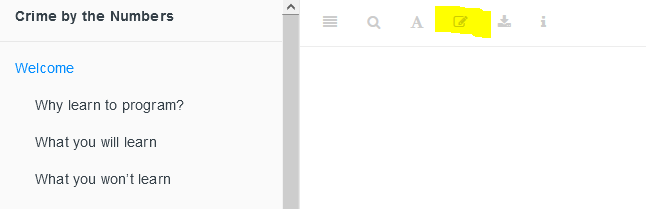
\includegraphics[width=1\linewidth,height=0.45\textheight,]{images/edit_button} \end{center}

Please only use the above two methods to contribute or make
suggestions about the book. Don't email me. While it's a bit
more work for you to do it this way, since you'll need to
make a GitHub account if you don't already have one, it
helps me. I wrote this book, in part, to help my career so
having evidence that people read it and are contributing to
it is important to me. It's a way to publicly measure the
book's impact.

\hypertarget{where-to-find-data-included-in-this-book}{%
\section*{Where to find data included in this
book}\label{where-to-find-data-included-in-this-book}}
\addcontentsline{toc}{section}{Where to find data included
in this book}

To download the data used in this book please see
\href{https://github.com/jacobkap/r4crimz/tree/master/data}{here.}
Each of the files that are used in this book are available
to download at that link. At the top of every chapter that
uses one of these files I'll say exactly which file(s) you
need to download. The best way to use this book is to follow
along by downloading the data and running the code that I
include in each chapter.

\hypertarget{where-to-find-code-included-in-this-book}{%
\section*{Where to find code included in this
book}\label{where-to-find-code-included-in-this-book}}
\addcontentsline{toc}{section}{Where to find code included
in this book}

If you're reading this book through its
\href{https://crimebythenumbers.com}{website,} you can
easily copy the code by clicking on the ``Copy to
clipboard'' option on the top right of every chunk of code.
This button, shown in the image below, will copy all of the
code in the chunk and you can then paste (through
Control/Command+V) into R.

\begin{center}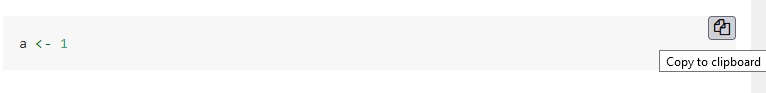
\includegraphics[width=1\linewidth,height=0.45\textheight,]{images/copy_code} \end{center}

I've also made each chapter available to download as an R
file that has every line of code used in each chapter
available to you to run. To download the files, please go to
the book's GitHub page
\href{https://github.com/jacobkap/crimebythenumbers/tree/master/code_repository}{here.}
I've saved each chapter twice - once where it only includes
the code used (in the ``just\_code'' folder) and once where
it includes the code and all of the text in the chapter (in
the ``code\_and\_text'' folder). So download whichever one
you want to use. The code is identical in each.

\hypertarget{about-the-author}{%
\chapter*{About the author}\label{about-the-author}}
\addcontentsline{toc}{chapter}{About the author}

\textbf{Jacob Kaplan} is the a researcher at the Princeton
School of Public and International Affairs. He holds a PhD
from the University of Pennsylvania.

He is the author of several R packages that make it easier
to work with data, including
\href{https://jacobkap.github.io/fastDummies/}{fastDummies}
and
\href{https://jacobkap.github.io/asciiSetupReader/}{asciiSetupReader.}
His \href{http://jacobdkaplan.com/}{website} allows easy
analysis of crime-related data, and he has released over a
\href{http://jacobdkaplan.com/data.html}{dozen crime data
sets} that he has compiled, cleaned, and made available to
the public. He is also the author of books on the two
primary criminal justice data sets: the FBI's
\href{https://ucrbook.com/}{Uniform Crime Reporting (UCR)
Program Data} and the FBI's
\href{https://nibrsbook.com/}{National Incident Based
Reporting System (NIBRS)} data.

\mainmatter

\hypertarget{part-introduction}{%
\chapter*{(PART) Introduction}\label{part-introduction}}
\addcontentsline{toc}{chapter}{(PART) Introduction}

\hypertarget{a-soup-to-nuts-project-example}{%
\chapter{A soup to nuts project
example}\label{a-soup-to-nuts-project-example}}

Before we get into exactly how to use R, we'll go over a
brief example of a kind of data project that you'd do in the
real world. For this chapter we'll look at FBI homicide data
that you can download
\href{https://github.com/jacobkap/r4crimz/tree/master/data}{here.}
The file is called ``shr\_1976\_2020.rds''.

\hypertarget{big-picture-data-example}{%
\section{Big picture data
example}\label{big-picture-data-example}}

Below is a large chunk of R code along with some comments
about what the code does. The purpose of this example is to
show that with relatively little code (excluding blank lines
and comments, there are only 35 lines of R code here) you
can go from opening a data set to making a graph that
answers your research question. I don't expect you to
understand any of this code as it is fairly complex and
involves many different concepts in programming. So if the
code is scary - and for many early programmers seeing a
bunch of code that you don't understand is scary and
overwhelming - feel free to ignore the code itself.

We'll cover each of these skills in turn throughout the book
so that by the end of the book you should be able to come
back and understand the code (and modify it to meet your own
needs). The important thing is that you can see exactly what
R can do (and this is only a tiny example of R's
flexibility) and think about the process to get there (which
we'll talk about below).

At the time of this writing, the FBI had just released 2020
crime data, which showed about a 30\% increase in murders
relative to 2019. This had led to an explosion of (in my
opinion highly premature) explanations of why exactly murder
went up so much in 2020. A common explanation is that it is
largely driven by gun violence among gang members who are
killing each other in a cyclical pattern of murders followed
by retaliatory murders. For our coding example, we'll
examine that claim by seeing if gang violence did indeed
increase, and whether it increased more than other types of
murders.

The end result is the graph below. It is, in my opinion, a
fairly strong answer to our question. It shows the percent
change in murders by the victim-offender relationship from
2019 to 2020. This is using FBI murder data, which
technically does have a variable that says if the murder is
gang related, but it's a very flawed variable (i.e.~vast
undercount of gang-related murders) so I prefer to use
stranger and acquaintance murders as a rough proxy. And we
now have an easy to read graph that shows that while indeed
stranger and acquaintance murders did go up a lot, nearly
all relationship groups experienced far more murders in 2020
than in 2019. This suggests that there was a broad increase
in murder in 2020, and it was not driven merely by an
increase in one or a few groups.

\begin{center}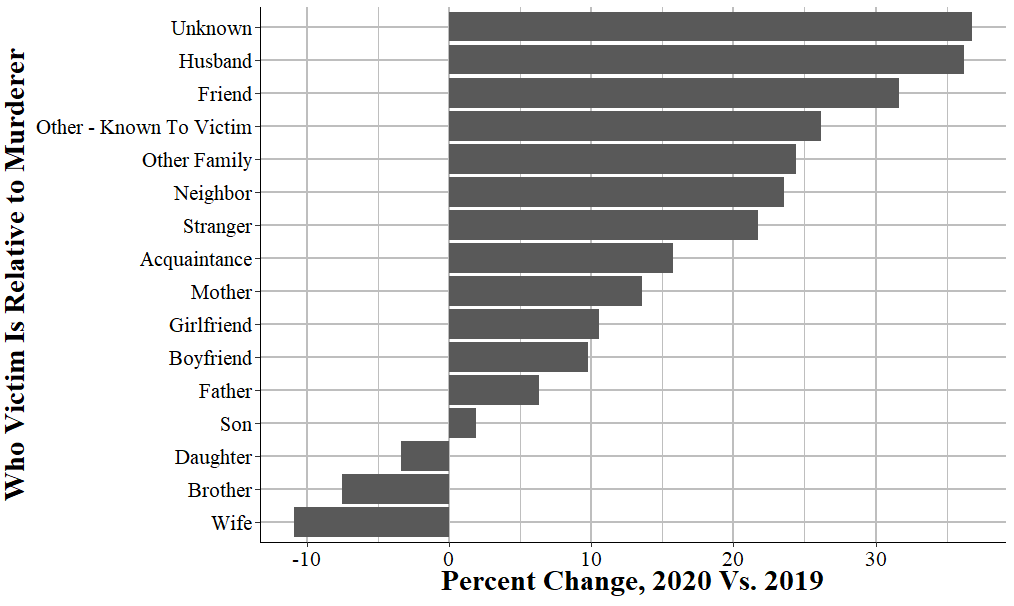
\includegraphics[width=1\linewidth,height=0.45\textheight,]{images/shr_motivation_example} \end{center}

These graphs (though modified to a table instead of a graph)
were included in a article I contributed to on the site
\href{https://fivethirtyeight.com/features/murders-spiked-in-2020-how-will-that-change-the-politics-of-crime/}{FiveThirtyEight}
in discussing the murder increase in 2020. So this is an
actual work product that is used in a major media
publication - and is something that you'll be able to do by
the end of this book. For nearly all research you do you'll
follow the same process as in this example: load data into
R, clean it somehow, and create a graph or a table or do a
regression on it. While this can range from very simple to
very complex depending on your exact situation (and how
clean the data is that you start with), all research
projects are essentially the same.

Please look at the following large chunk of code. We'll next
go through each of the different pieces of this code to
start understanding how they work. Throughout the course of
this book we'll cover these steps in more detail - as most
research programming work follows the same process - so here
we'll talk more abstractly about what each does. The goal is
for you to understand the basic steps necessary for using R
to do research, and to understand how R can do it - but not
having to understand what each line of code does just yet.

\begin{Shaded}
\begin{Highlighting}[]
\FunctionTok{library}\NormalTok{(dplyr) }\CommentTok{\# Used to aggregate data}
\FunctionTok{library}\NormalTok{(ggplot2) }\CommentTok{\# Used to make the graph}
\CommentTok{\# Warning: package \textquotesingle{}ggplot2\textquotesingle{} was built under R version 4.1.3}
\FunctionTok{library}\NormalTok{(crimeutils) }\CommentTok{\# Used to capitalize words in a column}
\FunctionTok{library}\NormalTok{(tidyr) }\CommentTok{\# Used to reshape the data}

\CommentTok{\# Load in the data}
\NormalTok{shr }\OtherTok{\textless{}{-}} \FunctionTok{readRDS}\NormalTok{(}\StringTok{"data/shr\_1976\_2020.rds"}\NormalTok{)}

\CommentTok{\# See which agencies reported in 2019 and 2020}
\CommentTok{\# An "ori" is a unique identifier code for agencies in FBI data}
\NormalTok{agencies\_2019 }\OtherTok{\textless{}{-}}\NormalTok{ shr}\SpecialCharTok{$}\NormalTok{ori[shr}\SpecialCharTok{$}\NormalTok{year }\SpecialCharTok{==} \DecValTok{2019}\NormalTok{]}
\NormalTok{agencies\_2020 }\OtherTok{\textless{}{-}}\NormalTok{ shr}\SpecialCharTok{$}\NormalTok{ori[shr}\SpecialCharTok{$}\NormalTok{year }\SpecialCharTok{==} \DecValTok{2020}\NormalTok{]}
\CommentTok{\# Get which agencies reported in both years so we have an}
\CommentTok{\# apples{-}to{-}apples comparison}
\NormalTok{agencies\_in\_both }\OtherTok{\textless{}{-}}\NormalTok{ agencies\_2019[agencies\_2019 }\SpecialCharTok{\%in\%}\NormalTok{ agencies\_2020]}

\CommentTok{\# Keep just data from 2019 and 2020 and where the agencies}
\CommentTok{\# is one of the agencies chosen above. Also keep only murder and}
\CommentTok{\# nonnegligent manslaughter (so excluding  negligent manslaughter).}
\NormalTok{shr\_2019\_2020 }\OtherTok{\textless{}{-}}\NormalTok{ shr[shr}\SpecialCharTok{$}\NormalTok{year }\SpecialCharTok{\%in\%} \DecValTok{2019}\SpecialCharTok{:}\DecValTok{2020}\NormalTok{, ]}
\NormalTok{shr\_2019\_2020 }\OtherTok{\textless{}{-}}\NormalTok{ shr\_2019\_2020[shr\_2019\_2020}\SpecialCharTok{$}\NormalTok{ori }\SpecialCharTok{\%in\%}
\NormalTok{  agencies\_in\_both, ]}
\NormalTok{shr\_2019\_2020 }\OtherTok{\textless{}{-}}\NormalTok{ shr\_2019\_2020[shr\_2019\_2020}\SpecialCharTok{$}\NormalTok{homicide\_type }\SpecialCharTok{\%in\%}
  \StringTok{"murder and nonnegligent manslaughter"}\NormalTok{, ]}

\CommentTok{\# Get the number of murders by victim{-}offender relationship in 2019 and 2020}
\CommentTok{\# Then find the percent change in murders by this group from 2019 to 2020}
\CommentTok{\# Sort data by smallest to largest percent change}
\NormalTok{shr\_difference }\OtherTok{\textless{}{-}}
\NormalTok{  shr\_2019\_2020 }\SpecialCharTok{\%\textgreater{}\%}
  \FunctionTok{group\_by}\NormalTok{(year) }\SpecialCharTok{\%\textgreater{}\%}
  \FunctionTok{count}\NormalTok{(victim\_1\_relation\_to\_offender\_1) }\SpecialCharTok{\%\textgreater{}\%}
  \FunctionTok{spread}\NormalTok{(year, n) }\SpecialCharTok{\%\textgreater{}\%}
  \FunctionTok{mutate}\NormalTok{(}
    \AttributeTok{difference =} \StringTok{\textasciigrave{}}\AttributeTok{2020}\StringTok{\textasciigrave{}} \SpecialCharTok{{-}} \StringTok{\textasciigrave{}}\AttributeTok{2019}\StringTok{\textasciigrave{}}\NormalTok{,}
    \AttributeTok{percent\_change =}\NormalTok{ difference }\SpecialCharTok{/} \StringTok{\textasciigrave{}}\AttributeTok{2019}\StringTok{\textasciigrave{}} \SpecialCharTok{*} \DecValTok{100}\NormalTok{,}
    \AttributeTok{victim\_1\_relation\_to\_offender\_1 =}
      \FunctionTok{capitalize\_words}\NormalTok{(victim\_1\_relation\_to\_offender\_1)}
\NormalTok{  ) }\SpecialCharTok{\%\textgreater{}\%}
  \FunctionTok{filter}\NormalTok{(}\StringTok{\textasciigrave{}}\AttributeTok{2019}\StringTok{\textasciigrave{}} \SpecialCharTok{\textgreater{}=} \DecValTok{50}\NormalTok{) }\SpecialCharTok{\%\textgreater{}\%}
  \FunctionTok{arrange}\NormalTok{(percent\_change)}

\CommentTok{\# This is only for the graph. By default graphs order alphabetically}
\CommentTok{\# but this makes sure it orders it based on the ordering we made above}
\CommentTok{\# (smallest to largest percent change)}
\NormalTok{shr\_difference}\SpecialCharTok{$}\NormalTok{victim\_1\_relation\_to\_offender\_1 }\OtherTok{\textless{}{-}}
  \FunctionTok{factor}\NormalTok{(shr\_difference}\SpecialCharTok{$}\NormalTok{victim\_1\_relation\_to\_offender\_1,}
    \AttributeTok{levels =}\NormalTok{ shr\_difference}\SpecialCharTok{$}\NormalTok{victim\_1\_relation\_to\_offender\_1}
\NormalTok{  )}

\CommentTok{\# Makes a barplot showing the percent change from 2019 to 2020 in number}
\CommentTok{\# of murders by victim group. Labels the x{-}axis and the y{-}axis, shifts}
\CommentTok{\# the graph so that relationship labels are on the y{-}axis for easy reading.}
\CommentTok{\# And finally uses the "crim" theme that changes the colors in the graph to}
\CommentTok{\# make it a little easier to see.}
\FunctionTok{ggplot}\NormalTok{(shr\_difference, }\FunctionTok{aes}\NormalTok{(}
  \AttributeTok{x =}\NormalTok{ victim\_1\_relation\_to\_offender\_1,}
  \AttributeTok{y =}\NormalTok{ percent\_change}
\NormalTok{)) }\SpecialCharTok{+}
  \FunctionTok{geom\_bar}\NormalTok{(}\AttributeTok{stat =} \StringTok{"identity"}\NormalTok{) }\SpecialCharTok{+}
  \FunctionTok{ylab}\NormalTok{(}\StringTok{"\% Change, 2020 Vs. 2019"}\NormalTok{) }\SpecialCharTok{+}
  \FunctionTok{xlab}\NormalTok{(}\StringTok{"Who Victim Is Relative to Murderer"}\NormalTok{) }\SpecialCharTok{+}
  \FunctionTok{coord\_flip}\NormalTok{() }\SpecialCharTok{+}
  \FunctionTok{theme\_crim}\NormalTok{()}
\end{Highlighting}
\end{Shaded}

\begin{center}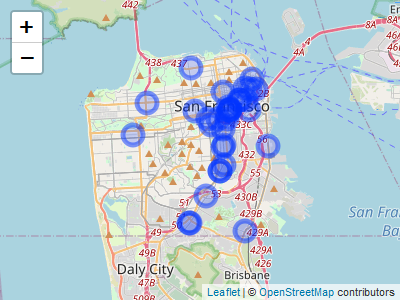
\includegraphics[width=1\linewidth,height=0.45\textheight,]{crimebythenumbers_files/figure-latex/unnamed-chunk-7-1} \end{center}

\hypertarget{little-picture-data-example}{%
\section{Little picture data
example}\label{little-picture-data-example}}

We'll now look at each piece of the larger chunk of code
above, and I'll explain what it does. There are five
different steps that I take to create the graph from the
data we use:

\begin{enumerate}
\def\labelenumi{\arabic{enumi}.}
\tightlist
\item
  Load the packages we use
\item
  Load the data
\item
  Clean the data
\item
  Aggregate the data
\item
  Make the graph
\end{enumerate}

\hypertarget{loading-packages}{%
\subsection{Loading packages}\label{loading-packages}}

In R we'll often use code written by other people that have
tools that we want to use in our code. To use this code we
need to tell R that we want to use that particular package -
and packages are just a collection of other people's code. A
collection of code for a specific purpose (e.g.~making a
graph, doing a very particular cleaning task) is called a
function. Each package is a collection of functions. For
this example, we're using packages that help us clean and
aggregate data or to graph it, so we load it here. The
general convention is to start your R file with each of the
packages you want to use at the top of the file.

\begin{Shaded}
\begin{Highlighting}[]
\FunctionTok{library}\NormalTok{(dplyr)}
\FunctionTok{library}\NormalTok{(ggplot2)}
\FunctionTok{library}\NormalTok{(crimeutils)}
\FunctionTok{library}\NormalTok{(tidyr)}
\end{Highlighting}
\end{Shaded}

\hypertarget{loading-data}{%
\subsection{Loading data}\label{loading-data}}

Next we need to load in our data. The data we're using is a
type of R data file called an .Rds file so we load it using
the function \texttt{readRDS()}, which is one of the
functions built into R so we don't actually need to use any
package for it. For this example, we're using data from the
FBI's Supplementary Homicide Report which are an annual data
set that has relatively detailed information on most (but
not all, as not all agencies report data) murders in the
United States. This includes the relationship between the
victim and the offender (technically the suspected offender)
in the murder, which is what we'll look at. When we read in
the data to R we need to give it a name so R knows what it
is called. We'll call this data ``shr'' since that is the
normal abbreviation for the Supplementary Homicide Report
data. Normally in R we use lower cased letters when naming
something, which is why we're calling it ``shr'' rather than
``SHR.''

Each row of data is actually a murder incident, and there
can be up to 11 victims per murder incident. So we'll be
undercounting murders as in this example we're only looking
at the first victim in an incident. But, as it's an example,
this is fine as I don't want it to be too complicated and
including more than just the first victim would greatly
complicate our code.

\begin{Shaded}
\begin{Highlighting}[]
\NormalTok{shr }\OtherTok{\textless{}{-}} \FunctionTok{readRDS}\NormalTok{(}\StringTok{"data/shr\_1976\_2020.rds"}\NormalTok{)}
\end{Highlighting}
\end{Shaded}

\hypertarget{cleaning}{%
\subsection{Cleaning}\label{cleaning}}

One of the annoying quirks of dealing with FBI data is that
different agencies report each year. So comparing different
years has an issue because you'll be doing an
apples-to-oranges competition as an agency may report one
year but not another. So for this data the first thing we
need to do is to make sure we're only looking at agencies
that reported data in both years. The first few lines check
which agencies reported in 2019 and which agencies reported
in 2020. We do this by looking at which ORIs (in the ``ori''
column) are present in each year (as agencies that did not
report won't be in the data). An ORI is the FBI term for a
unique ID for that agency. Then we make a vector, which has
only the ORIs that are present in both years.

We then subset the data to only data from 2019 and 2020 and
where the agency reported in both years. Subsetting
essentially means that we only keep the rows of data that
meet those conditions. Another quirk of this data is that it
includes homicides that are not murder - namely, negligent
manslaughter. So the final subsetting condition we use is
that it only includes murder and nonnegligent manslaughter.

\begin{Shaded}
\begin{Highlighting}[]
\NormalTok{agencies\_2019 }\OtherTok{\textless{}{-}}\NormalTok{ shr}\SpecialCharTok{$}\NormalTok{ori[shr}\SpecialCharTok{$}\NormalTok{year }\SpecialCharTok{==} \DecValTok{2019}\NormalTok{]}
\NormalTok{agencies\_2020 }\OtherTok{\textless{}{-}}\NormalTok{ shr}\SpecialCharTok{$}\NormalTok{ori[shr}\SpecialCharTok{$}\NormalTok{year }\SpecialCharTok{==} \DecValTok{2020}\NormalTok{]}
\NormalTok{agencies\_in\_both }\OtherTok{\textless{}{-}}\NormalTok{ agencies\_2019[agencies\_2019 }\SpecialCharTok{\%in\%}\NormalTok{ agencies\_2020]}


\NormalTok{shr\_2019\_2020 }\OtherTok{\textless{}{-}}\NormalTok{ shr[shr}\SpecialCharTok{$}\NormalTok{year }\SpecialCharTok{\%in\%} \DecValTok{2019}\SpecialCharTok{:}\DecValTok{2020}\NormalTok{, ]}
\NormalTok{shr\_2019\_2020 }\OtherTok{\textless{}{-}}\NormalTok{ shr\_2019\_2020[shr\_2019\_2020}\SpecialCharTok{$}\NormalTok{ori }\SpecialCharTok{\%in\%}\NormalTok{ agencies\_in\_both, ]}
\NormalTok{shr\_2019\_2020 }\OtherTok{\textless{}{-}}\NormalTok{ shr\_2019\_2020[shr\_2019\_2020}\SpecialCharTok{$}\NormalTok{homicide\_type }\SpecialCharTok{\%in\%}
  \StringTok{"murder and nonnegligent manslaughter"}\NormalTok{, ]}
\end{Highlighting}
\end{Shaded}

\hypertarget{aggregating}{%
\subsection{Aggregating}\label{aggregating}}

Now we have only the rows of data that we want. Each row of
data is a single murder incident, so we want to aggregate
that data to the year-level and see how many murders there
were for each victim-offender relationship group. The
following chunk of code does that and then finds the percent
difference. Since we can have large percent changes due to
low base rates, we then remove any rows where there were
fewer than 50 murders of that victim-offender relationship
type in 2019. Finally, we arrange the data from smallest to
largest difference. We'll print out the data just to show
you what it looks like.

\begin{Shaded}
\begin{Highlighting}[]
\NormalTok{shr\_difference }\OtherTok{\textless{}{-}}
\NormalTok{  shr\_2019\_2020 }\SpecialCharTok{\%\textgreater{}\%}
  \FunctionTok{group\_by}\NormalTok{(year) }\SpecialCharTok{\%\textgreater{}\%}
  \FunctionTok{count}\NormalTok{(victim\_1\_relation\_to\_offender\_1) }\SpecialCharTok{\%\textgreater{}\%}
  \FunctionTok{spread}\NormalTok{(year, n) }\SpecialCharTok{\%\textgreater{}\%}
  \FunctionTok{mutate}\NormalTok{(}
    \AttributeTok{difference =} \StringTok{\textasciigrave{}}\AttributeTok{2020}\StringTok{\textasciigrave{}} \SpecialCharTok{{-}} \StringTok{\textasciigrave{}}\AttributeTok{2019}\StringTok{\textasciigrave{}}\NormalTok{,}
    \AttributeTok{percent\_change =}\NormalTok{ difference }\SpecialCharTok{/} \StringTok{\textasciigrave{}}\AttributeTok{2019}\StringTok{\textasciigrave{}} \SpecialCharTok{*} \DecValTok{100}\NormalTok{,}
    \AttributeTok{victim\_1\_relation\_to\_offender\_1 =}
      \FunctionTok{capitalize\_words}\NormalTok{(victim\_1\_relation\_to\_offender\_1)}
\NormalTok{  ) }\SpecialCharTok{\%\textgreater{}\%}
  \FunctionTok{filter}\NormalTok{(}\StringTok{\textasciigrave{}}\AttributeTok{2019}\StringTok{\textasciigrave{}} \SpecialCharTok{\textgreater{}=} \DecValTok{50}\NormalTok{) }\SpecialCharTok{\%\textgreater{}\%}
  \FunctionTok{arrange}\NormalTok{(percent\_change)}
\NormalTok{shr\_difference}
\CommentTok{\# \# A tibble: 16 x 5}
\CommentTok{\#    victim\_1\_relation\_to\_offe\textasciitilde{}1 \textasciigrave{}2019\textasciigrave{} \textasciigrave{}2020\textasciigrave{} diffe\textasciitilde{}2 perce\textasciitilde{}3}
\CommentTok{\#    \textless{}chr\textgreater{}                        \textless{}int\textgreater{}  \textless{}int\textgreater{}   \textless{}int\textgreater{}   \textless{}dbl\textgreater{}}
\CommentTok{\#  1 Wife                           330    294     {-}36  {-}10.9 }
\CommentTok{\#  2 Brother                         93     86      {-}7   {-}7.53}
\CommentTok{\#  3 Daughter                        89     86      {-}3   {-}3.37}
\CommentTok{\#  4 Son                            157    160       3    1.91}
\CommentTok{\#  5 Father                          95    101       6    6.32}
\CommentTok{\#  6 Boyfriend                      164    180      16    9.76}
\CommentTok{\#  7 Girlfriend                     390    431      41   10.5 }
\CommentTok{\#  8 Mother                         118    134      16   13.6 }
\CommentTok{\#  9 Acquaintance                  1494   1729     235   15.7 }
\CommentTok{\# 10 Stranger                      1549   1886     337   21.8 }
\CommentTok{\# 11 Neighbor                        85    105      20   23.5 }
\CommentTok{\# 12 Other Family                   209    260      51   24.4 }
\CommentTok{\# 13 Other {-} Known To Victim        757    955     198   26.2 }
\CommentTok{\# 14 Friend                         272    358      86   31.6 }
\CommentTok{\# 15 Husband                         58     79      21   36.2 }
\CommentTok{\# 16 Unknown                       6216   8504    2288   36.8 }
\CommentTok{\# \# ... with abbreviated variable names}
\CommentTok{\# \#   1: victim\_1\_relation\_to\_offender\_1, 2: difference,}
\CommentTok{\# \#   3: percent\_change}
\end{Highlighting}
\end{Shaded}

\hypertarget{graphing}{%
\subsection{Graphing}\label{graphing}}

Once we have our data cleaned and organized in the way we
want, we are ready to graph it. By default when R graphs
data it will organize it alphabetically. In our case we want
it ordered by smallest to largest change in the number of
murders between 2019 and 2020 by relationship type. So we
first tell R to order it by the relationship type variable,
which we've already sorted in the last section of code. Then
we use the \texttt{ggplot()} function (which is covered
extensively in Chapters @ref(graphing-intro) and
@ref(ois-graphs)) to make our graph. In our code we include
the data set we're using, which is the shr\_difference data
and the columns we want to graph. Then we tell it we want to
create a bar chart and what we want the x-axis and y-axis
labels to be. Finally, we have two lines that just affect
how the graph looks. All of this is covered in the two
graphing chapters, but is only several lines of code to go
from cleaned data to a beautiful - and informative -
graphic.

\begin{Shaded}
\begin{Highlighting}[]
\NormalTok{shr\_difference}\SpecialCharTok{$}\NormalTok{victim\_1\_relation\_to\_offender\_1 }\OtherTok{\textless{}{-}}
  \FunctionTok{factor}\NormalTok{(shr\_difference}\SpecialCharTok{$}\NormalTok{victim\_1\_relation\_to\_offender\_1,}
    \AttributeTok{levels =}\NormalTok{ shr\_difference}\SpecialCharTok{$}\NormalTok{victim\_1\_relation\_to\_offender\_1}
\NormalTok{  )}

\FunctionTok{ggplot}\NormalTok{(shr\_difference, }\FunctionTok{aes}\NormalTok{(}
  \AttributeTok{x =}\NormalTok{ victim\_1\_relation\_to\_offender\_1,}
  \AttributeTok{y =}\NormalTok{ percent\_change}
\NormalTok{)) }\SpecialCharTok{+}
  \FunctionTok{geom\_bar}\NormalTok{(}\AttributeTok{stat =} \StringTok{"identity"}\NormalTok{) }\SpecialCharTok{+}
  \FunctionTok{ylab}\NormalTok{(}\StringTok{"\% Change, 2020 Vs. 2019"}\NormalTok{) }\SpecialCharTok{+}
  \FunctionTok{xlab}\NormalTok{(}\StringTok{"Who Victim Is Relative to Murderer"}\NormalTok{) }\SpecialCharTok{+}
  \FunctionTok{coord\_flip}\NormalTok{() }\SpecialCharTok{+}
  \FunctionTok{theme\_crim}\NormalTok{()}
\end{Highlighting}
\end{Shaded}

\begin{center}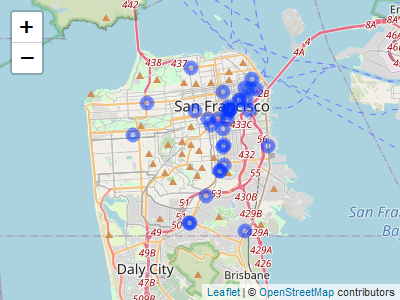
\includegraphics[width=1\linewidth,height=0.45\textheight,]{crimebythenumbers_files/figure-latex/unnamed-chunk-12-1} \end{center}

\hypertarget{reusing-and-modifying-code}{%
\section{Reusing and modifying
code}\label{reusing-and-modifying-code}}

One of the main benefits of programming is that once you
write code to do one thing, it's usually very easy to adapt
it to do a similar thing. Below I've copied some of the code
we used above and changed only one thing: instead of looking
at the column ``victim\_1\_relation\_to\_offender\_1'' we're
now looking at the column ``offender\_1\_weapon''. That's
all I did, everything else is identical. Now after about 30
seconds of copying and changing the column name, we have a
graph that shows weapon usage changes from 2019 to 2020
instead of victim-offender relationship.

This is one of the key benefits of programming over
something more click intensive like using Excel or
SPSS.\footnote{I'm aware that technically you can write SPSS
  code. However, every single person I know who has ever
  used SPSS does so by clicking buttons and is afraid of
  writing code.} There's certainly more upfront work than
just clicking buttons, but once we have working code we can
very quickly reuse it or modify it slightly.

\begin{Shaded}
\begin{Highlighting}[]
\NormalTok{shr\_difference }\OtherTok{\textless{}{-}}
\NormalTok{  shr\_2019\_2020 }\SpecialCharTok{\%\textgreater{}\%}
  \FunctionTok{group\_by}\NormalTok{(year) }\SpecialCharTok{\%\textgreater{}\%}
  \FunctionTok{count}\NormalTok{(offender\_1\_weapon) }\SpecialCharTok{\%\textgreater{}\%}
  \FunctionTok{spread}\NormalTok{(year, n) }\SpecialCharTok{\%\textgreater{}\%}
  \FunctionTok{mutate}\NormalTok{(}
    \AttributeTok{difference =} \StringTok{\textasciigrave{}}\AttributeTok{2020}\StringTok{\textasciigrave{}} \SpecialCharTok{{-}} \StringTok{\textasciigrave{}}\AttributeTok{2019}\StringTok{\textasciigrave{}}\NormalTok{,}
    \AttributeTok{percent\_change =}\NormalTok{ difference }\SpecialCharTok{/} \StringTok{\textasciigrave{}}\AttributeTok{2019}\StringTok{\textasciigrave{}} \SpecialCharTok{*} \DecValTok{100}\NormalTok{,}
    \AttributeTok{offender\_1\_weapon =} \FunctionTok{capitalize\_words}\NormalTok{(offender\_1\_weapon)}
\NormalTok{  ) }\SpecialCharTok{\%\textgreater{}\%}
  \FunctionTok{filter}\NormalTok{(}\StringTok{\textasciigrave{}}\AttributeTok{2019}\StringTok{\textasciigrave{}} \SpecialCharTok{\textgreater{}=} \DecValTok{50}\NormalTok{) }\SpecialCharTok{\%\textgreater{}\%}
  \FunctionTok{arrange}\NormalTok{(percent\_change)}

\NormalTok{shr\_difference}\SpecialCharTok{$}\NormalTok{offender\_1\_weapon }\OtherTok{\textless{}{-}}
  \FunctionTok{factor}\NormalTok{(shr\_difference}\SpecialCharTok{$}\NormalTok{offender\_1\_weapon,}
    \AttributeTok{levels =}\NormalTok{ shr\_difference}\SpecialCharTok{$}\NormalTok{offender\_1\_weapon}
\NormalTok{  )}
\FunctionTok{ggplot}\NormalTok{(shr\_difference, }\FunctionTok{aes}\NormalTok{(}
  \AttributeTok{x =}\NormalTok{ offender\_1\_weapon,}
  \AttributeTok{y =}\NormalTok{ percent\_change}
\NormalTok{)) }\SpecialCharTok{+}
  \FunctionTok{geom\_bar}\NormalTok{(}\AttributeTok{stat =} \StringTok{"identity"}\NormalTok{) }\SpecialCharTok{+}
  \FunctionTok{ylab}\NormalTok{(}\StringTok{"\% Change, 2020 Vs. 2019"}\NormalTok{) }\SpecialCharTok{+}
  \FunctionTok{xlab}\NormalTok{(}\StringTok{"Offender Weapon"}\NormalTok{) }\SpecialCharTok{+}
  \FunctionTok{coord\_flip}\NormalTok{() }\SpecialCharTok{+}
  \FunctionTok{theme\_crim}\NormalTok{()}
\end{Highlighting}
\end{Shaded}

\begin{center}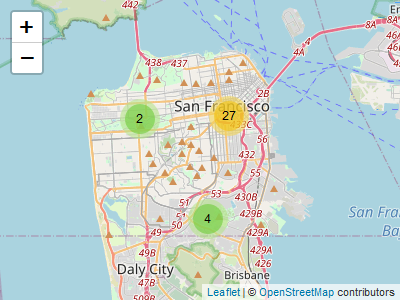
\includegraphics[width=1\linewidth,height=0.45\textheight,]{crimebythenumbers_files/figure-latex/unnamed-chunk-13-1} \end{center}

\hypertarget{intro-to-r}{%
\chapter{Introduction to R and RStudio}\label{intro-to-r}}

In this chapter you'll learn to open a data file in R. That
file is ``ucr2017.rda,'' which you'll need to download from
the data repository available
\href{https://github.com/jacobkap/r4crimz/tree/master/data}{here.}

\hypertarget{using-rstudio}{%
\section{Using RStudio}\label{using-rstudio}}

In this lesson we'll start by looking at RStudio then write
some brief code to load in some crime data and start
exploring it. This lesson will cover code that you won't
understand completely yet. That is fine, we'll cover
everything in more detail as the lessons progress.

RStudio is the interface we use to work with R. It has a
number of features to make it easier for us to work with R.
While not strictly necessary to use, most people who use R
do so through RStudio. When using R you don't need to open
up both R and RStudio on your computer. Just open RStudio
and it'll internally use R. We'll spend some time right now
looking at RStudio and the options you can change to make it
easier to use (and to suit your personal preferences with
appearance) as this will make all of the work that we do in
this book easier.

When you open up RStudio you'll see four panels, each of
which plays an important role in RStudio. Your RStudio may
not look like the setup I have in the following image - that
is fine, we'll learn how to change the appearance of RStudio
soon.

\begin{center}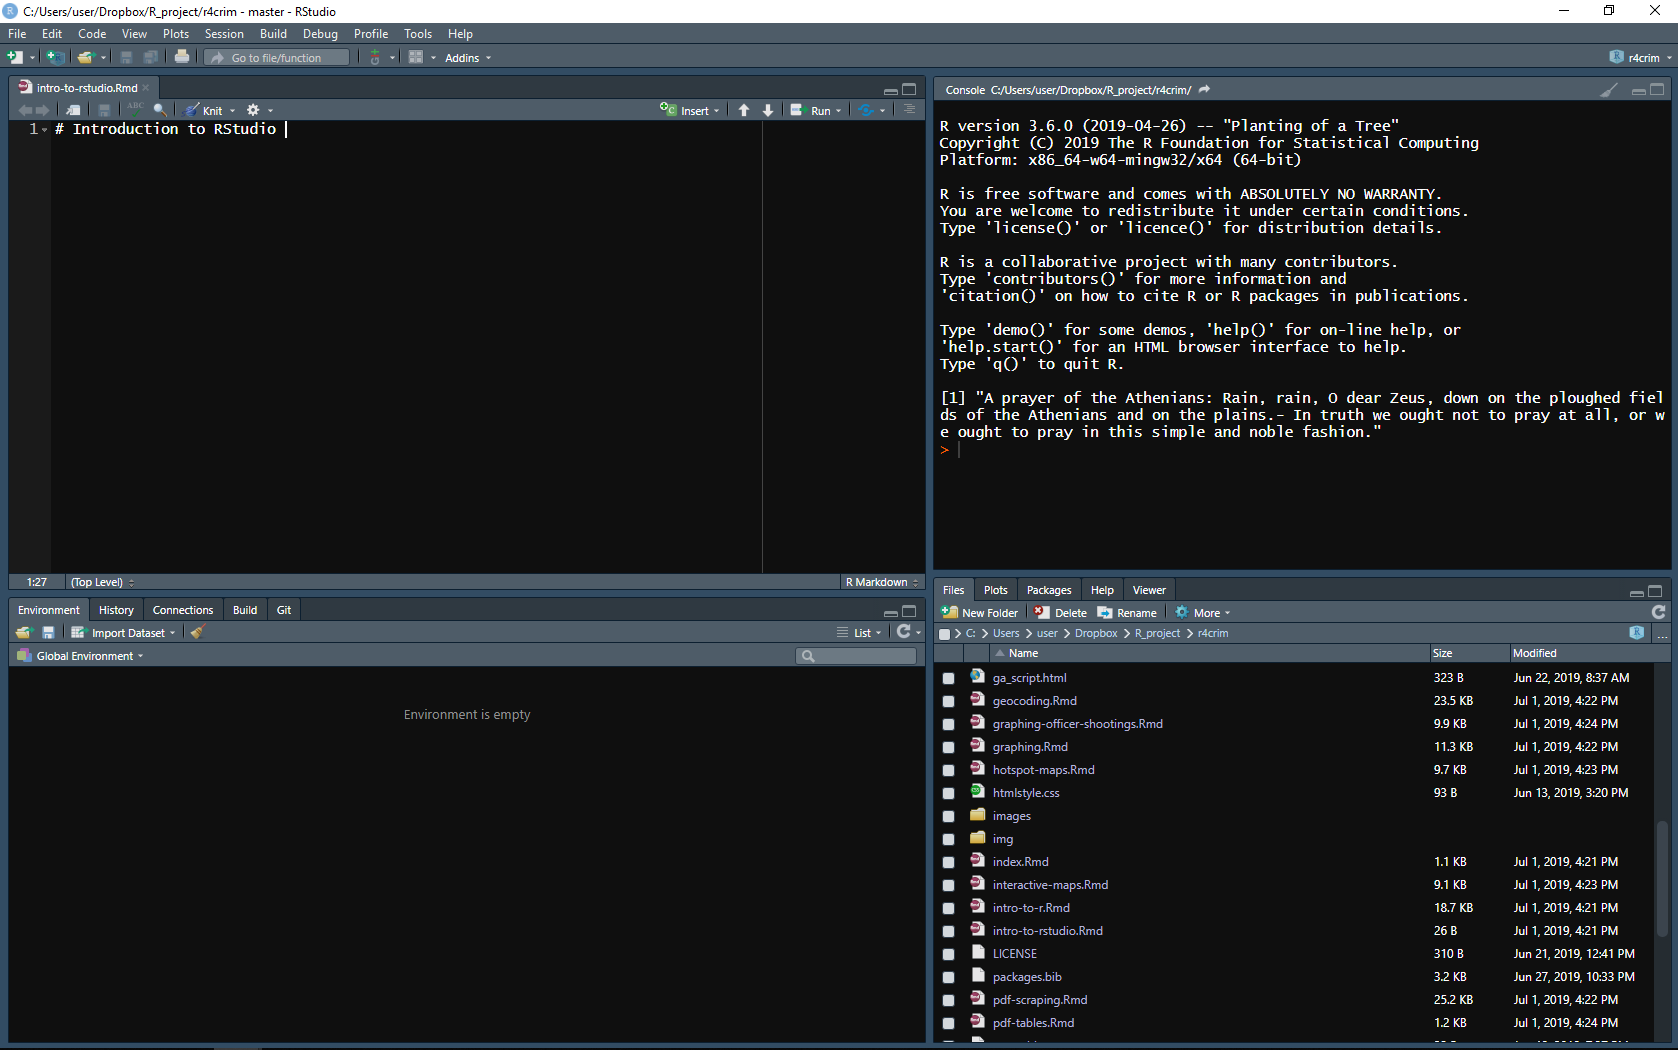
\includegraphics[width=1\linewidth,height=0.45\textheight,]{images/rstudio_1} \end{center}

At the top right of the image (and this may be in a
different location on your RStudio) is the Console panel.
Here you can write code, hit enter/return, and R will run
that code. If you write \texttt{2+2} it will return (in this
case that just mean it will print an answer) 4. This is
useful for doing something simple like using R as a
calculator or quickly looking at data. In most cases during
research this is where you'd do something that you don't
care to keep. This is because when you restart R it won't
save anything written in the Console. To do reproducible
research or to be able to collaborate with others you need a
way to keep the code you've written.

The way to keep the code you've written in a file that you
can open later or share with someone else is by writing code
in an R Script (if you're familiar with Stata, an R Script
is just like a .do file). An R Script is essentially a text
file (similar to a Word document) where you write code. To
run code in an R Script just click on a line of code or
highlight several lines and hit enter/return or click the
``Run'' button on the top right of the Source panel shown in
the top left of the above image. You'll see the lines of
code run in the Console and any output (if your code has an
output) will be shown there too (making a plot will be shown
in a different panel as we'll see soon).

For code that you don't want to run, called comments, start
the line with a pound sign \texttt{\#} and that line will
not be run (it will still print in the console if you run it
but it won't do anything). These comments should explain the
code you wrote (if it's not otherwise obvious what the code
does).

It is good practice to do all of your code writing in an R
Script - even if you delete some lines of code later - as it
eliminates the possibility of losing code or forgetting what
you wrote. Having all the code in front of you in a text
file also makes it easier to understand the flow of code
from start to finish for a task - an issue we'll discuss
more in later lessons.

While the Source and Console panels are the ones that are of
most use, there are two other panels worth discussing. As
these two panels let you interchange which tabs are
available in them, we'll return to them shortly in the
discussion of the options RStudio has to customize it.

\hypertarget{opening-an-r-script}{%
\subsection{Opening an R Script}\label{opening-an-r-script}}

When you want to open up a new R Script you can click File
on the very top left, then R Script. It will open up the
script in a new tab inside of the Source panel. There are
also a number of other file options available: R
Presentation which can make PowerPoints; R Markdown, which
can make Word Documents or PDFs that incorporate R code used
to make tables or graphs (and which we'll cover in Chapter
@ref(r-markdown)); and Shiny Web App to make websites using
R. There is too much to cover for an introductory book such
as this, but keep in mind the wide capabilities of R if you
have another task to do. To open an R Script that is already
saved to your computer, click ``Open File\ldots{}'' and
navigate to the file that you want to open.

\begin{center}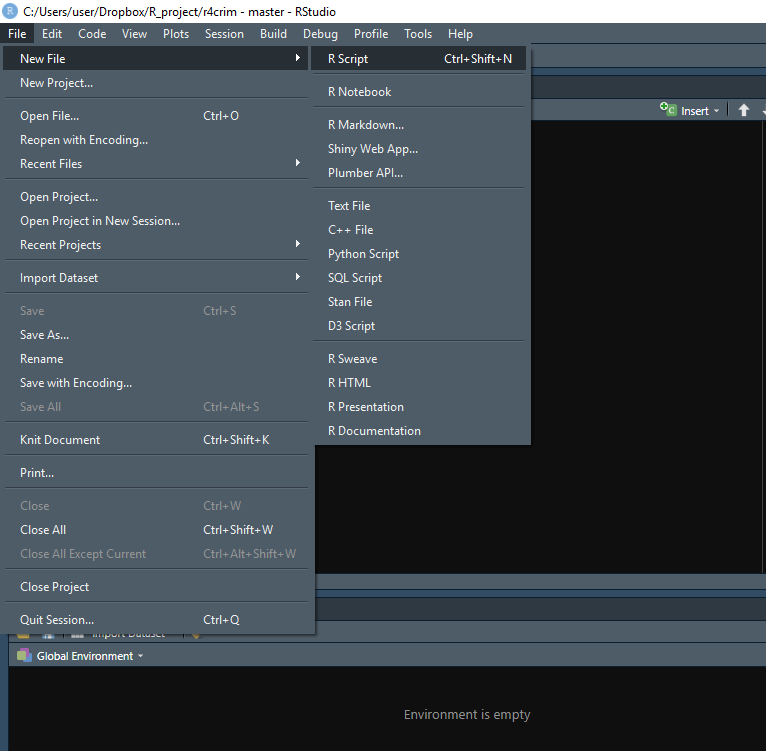
\includegraphics[width=1\linewidth,height=0.45\textheight,]{images/rstudio_2} \end{center}

\hypertarget{setting-the-working-directory}{%
\subsection{Setting the working
directory}\label{setting-the-working-directory}}

Many research projects incorporate data that someone else
(such as the FBI or a local police agency) has put together.
In these cases, we need to load the data into R to be able
to use it. In a little bit we'll load a data set into R and
start working on it, but let's take a step back now and
think about how to even load data. First, we'll need to get
the data onto our computer somehow, probably by downloading
it from an agency's website. Let's be specific - we don't
download it to our computer, we download it to a specific
folder on our computer (usually defaulted to the Downloads
folder on a Windows machine). So let's say you wanted to
load a file called ``data'' into R. If you have a file
called ``data'' in both your Desktop and your Downloads
folder, R wouldn't know which one you wanted. And unless
your data was in the folder R searches by default (which may
not be where the file is downloaded by default), R won't
know which file to load.

We need to tell R explicitly which folder has the data to
load. We do this by setting the ``Working Directory'' (or
the ``Folders where I want you, R, to look for my data'' in
more simple terms). To set a working directory in R click
the Session tab on the top menu, scroll to Set Working
Directory, then click Choose Directory. This will open a
window where you can navigate to the folder you want.

\begin{center}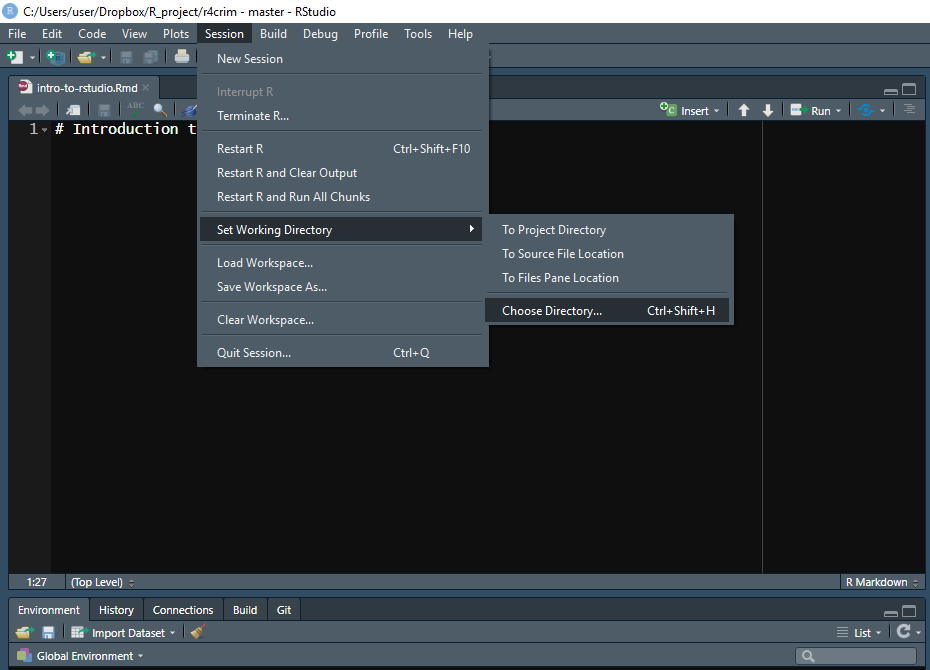
\includegraphics[width=1\linewidth,height=0.45\textheight,]{images/rstudio_3} \end{center}

After clicking Open in that window you'll see a new line of
code in the Console starting with \texttt{setwd()} and
inside of the parentheses is the route your computer takes
to get to the folder you selected. And now R knows which
folder to look in for the data you want. It is good form to
start your R Script with \texttt{setwd()} to make sure you
can load the data. Copy the line of code that says
\texttt{setwd()} (which stands for ``set working
directory''), including everything in the parentheses, to
your R Script when you start working.

\hypertarget{changing-rstudio}{%
\subsection{Changing RStudio}\label{changing-rstudio}}

Your RStudio looks different than my RStudio because I
changed a number of settings to suit my preferences. To do
so yourself click the Tools tab on the top menu and then
click Global Options.

\begin{center}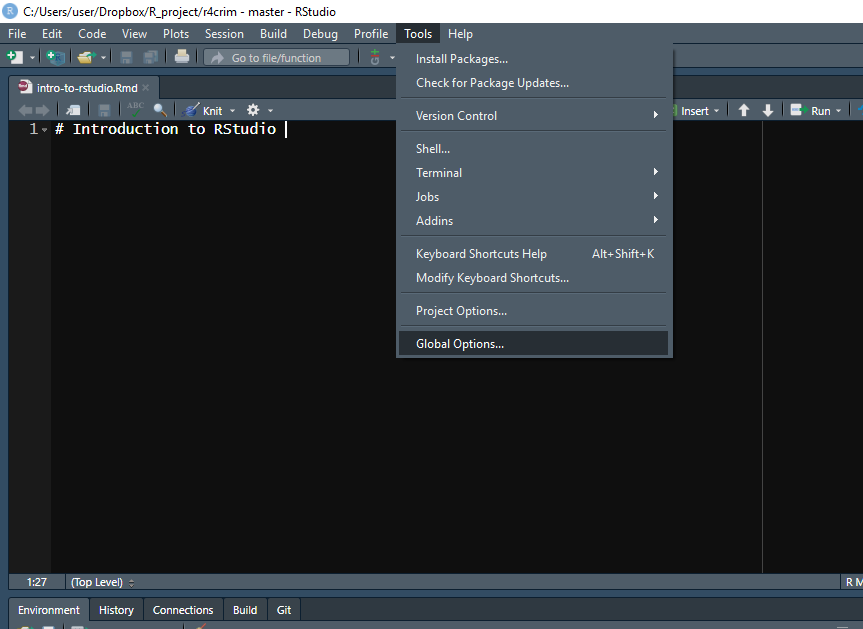
\includegraphics[width=1\linewidth,height=0.45\textheight,]{images/rstudio_5} \end{center}

This opens up a window with a number of different tabs to
change how R behaves and how it looks.

\hypertarget{general}{%
\subsubsection{General}\label{general}}

Under Workspace in the General tab make sure to
\textbf{uncheck} the ``Restore .RData into workspace at
startup'' and to set ``Save workspace to .RData on exit:''
to \textbf{Never}. What this does is make sure that every
time you open RStudio it starts fresh with no objects
(essentially data loaded into R or made in R) from previous
sessions. This may be annoying at times, especially when it
comes to loading large files, but the benefits far outweigh
the costs.

You want your code to run from start to finish without any
errors. Something I've seen many students do is write some
code in the Console (or in their R Script but out of order
of how it should be run) to fix an issue with the data. This
means their data is how it should be, but when the R session
restarts (such as if the computer restarts) they won't be
able to get back to that point. Making sure your code
handles everything from start to finish is well-worth the
avoided headache of trying to remember what code you did to
fix the issue previously.

\begin{center}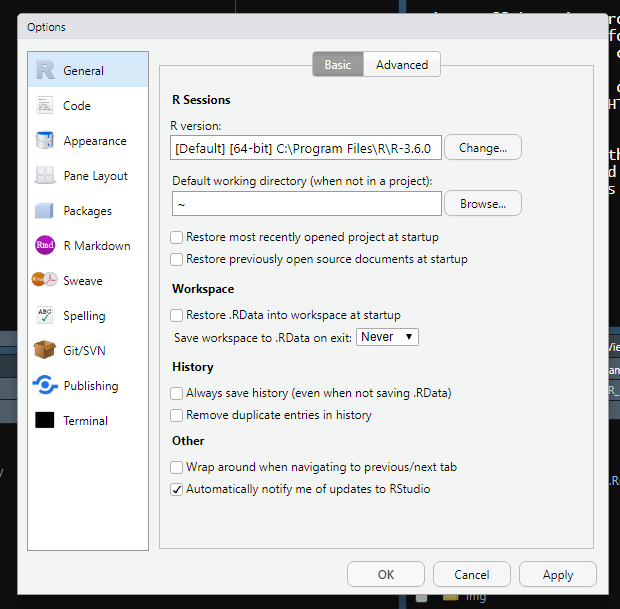
\includegraphics[width=1\linewidth,height=0.45\textheight,]{images/rstudio_6} \end{center}

\hypertarget{code}{%
\subsubsection{Code}\label{code}}

The Code tab lets you specify how you want the code to be
displayed. The important section for us is to make sure to
check the ``Soft-wrap R source files'' check-box. If you
write a very long line of code it gets too big to view all
at once and you must scroll to the right to read it all.
That can be annoying as you won't be able to see all the
code at once. Setting ``Soft-wrap'' makes it so if a line is
too long it will just be shown on multiple lines, which
solves that issue. In practice it is best to avoid long
lines of codes as it makes it hard to read, but that isn't
always possible.

\begin{center}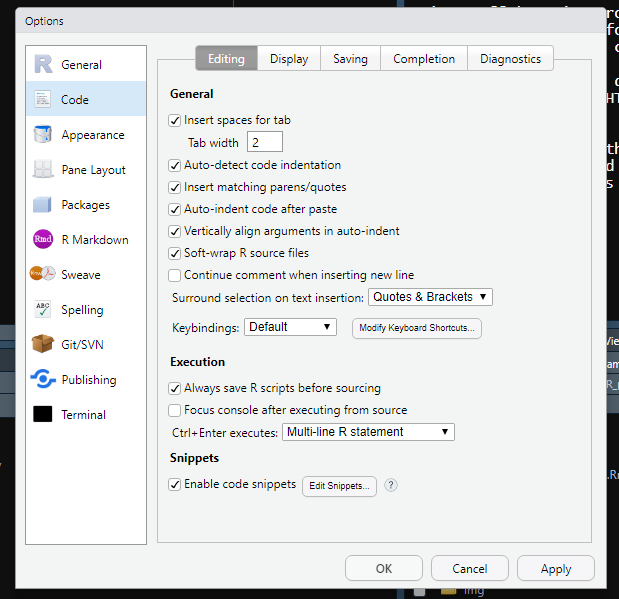
\includegraphics[width=1\linewidth,height=0.45\textheight,]{images/rstudio_7} \end{center}

\hypertarget{saving}{%
\paragraph{Saving}\label{saving}}

Inside of the Code tab we also want to turn on an option to
have RStudio automatically save the R script when we aren't
using it. This is like how Google Docs automatically saves
your document every second or so. While we should be saving
our file often (using the little floppy disk icon near the
top of RStudio), having RStudio automatically save adds a
level of security as it prevents losing a lot of progress if
we forget to save and RStudio crashes or we close it.

To set it to autosave, move to the Saving tab, and check the
``Automatically save when editor loses focus'' box. So if
you click out of RStudio or stop typing, it will
automatically save. You can also say how long to wait before
saving with options ranging from 500 milliseconds to 10,000
milliseconds, which is the same as 0.5 seconds to 10
seconds.

\begin{center}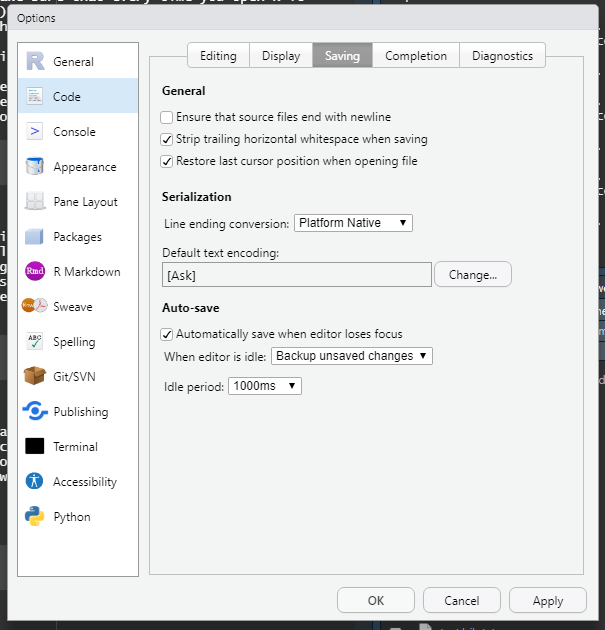
\includegraphics[width=1\linewidth,height=0.45\textheight,]{images/auto_save} \end{center}

\hypertarget{appearance}{%
\subsubsection{Appearance}\label{appearance}}

The Appearance tab lets you change the background, color,
and size of text. Change it to your preferences.

\begin{center}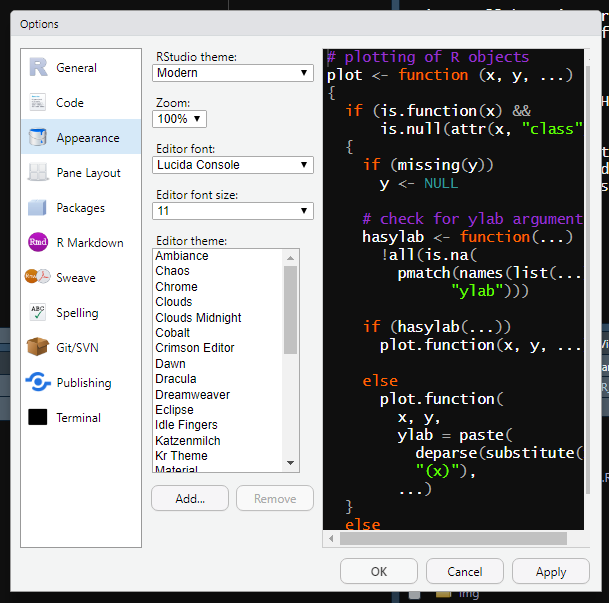
\includegraphics[width=1\linewidth,height=0.45\textheight,]{images/rstudio_8} \end{center}

\hypertarget{pane-layout}{%
\subsubsection{Pane Layout}\label{pane-layout}}

The final tab we'll look at is Pane Layout. This lets you
move around the Source, Console, and the other two panels.
There are a number of different tabs to select for the
panels (unchecking one just moves it to the other panel, it
doesn't remove it from RStudio), and we'll talk about three
of them. The Environment tab shows every object you load
into R or make in R. So if you load a file called ``data''
you can check the Environment tab. If it is there, you have
loaded the file correctly.

As we'll discuss more in Section @ref(functions-intro), the
Help tab will open up to show you a help page for a function
you want more information on (we'll also discuss exactly
what a function is below. But for now just think of a
function as a shortcut to using code that someone else
wrote). The Plots tab will display any plot you make. It
also keeps all plots you've made (until restarting RStudio)
so you can scroll through the plots.

\begin{center}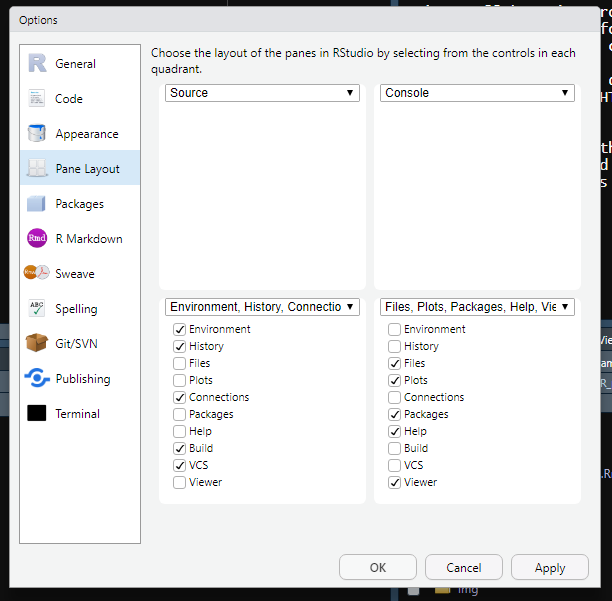
\includegraphics[width=1\linewidth,height=0.4\textheight,]{images/rstudio_9} \end{center}

\hypertarget{helpful-cheat-sheets}{%
\subsection{Helpful cheat
sheets}\label{helpful-cheat-sheets}}

RStudio also includes a number of links to helpful cheat
sheets for a few important topics. To get to it click Help,
then Cheatsheets, and click on whichever one you need.

\begin{center}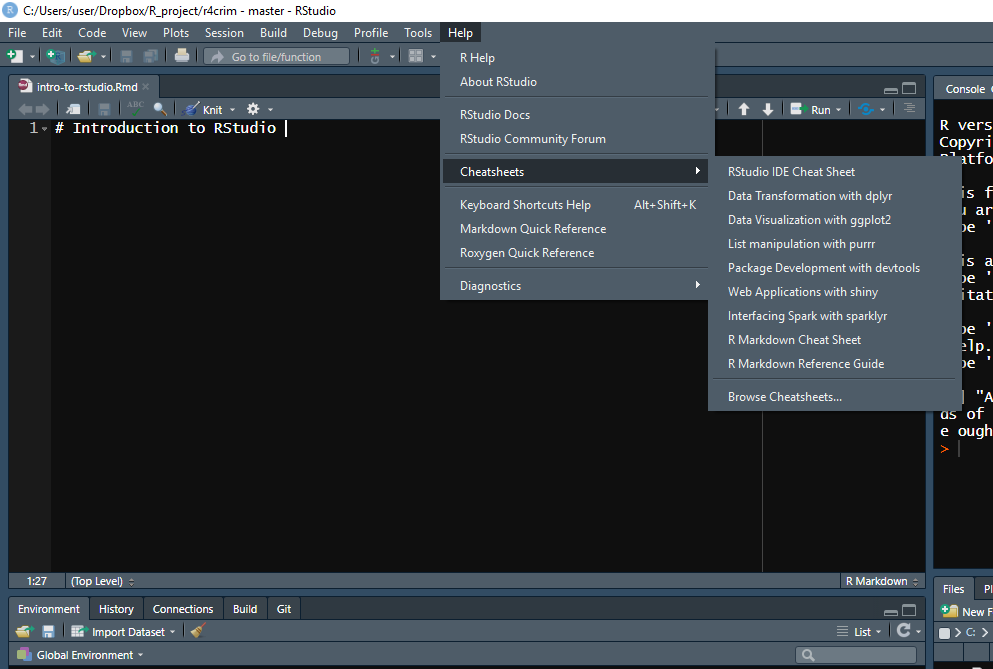
\includegraphics[width=1\linewidth,height=0.4\textheight,]{images/rstudio_4} \end{center}

\hypertarget{assignment}{%
\section{Assigning variables}\label{assignment}}

When we're using R for research the general process is to
load data, change it somehow (such as deleting rows we don't
want, aggregating from some small unit such as monthly crime
to a higher unit such as yearly crime), and then analyze it.
To do all this we need to be able to make sure each step we
do actually changes the data. This seems simple but is
actually a very common issue I've noticed when working with
new R programmers - they run code on the data (e.g.~deleting
certain rows) but forget to save the change to that data.

Let's look at an example of this. First, we need to know how
to create objects in R. I use ``object'' in a very vague
sense to mean anything that is loaded into R and can be
manipulated. To create something in R we assign
``something'' to an object name. This is a very technical
sentence so let's look at an example and then step back and
try to understand that sentence.

\begin{Shaded}
\begin{Highlighting}[]
\NormalTok{a }\OtherTok{\textless{}{-}} \DecValTok{1}
\end{Highlighting}
\end{Shaded}

Above I am creating the object ``a'' by assigning it the
value of 1. In R terms, ``a is assigned 1'' or ``a gets 1''.
In non-technical terms: a equals 1.

We can print out a to see if this is true.

\begin{Shaded}
\begin{Highlighting}[]
\NormalTok{a}
\CommentTok{\# [1] 1}
\end{Highlighting}
\end{Shaded}

When we print out a, it returns 1 since that was what a was
assigned to. We can assign a another value, and it will
overwrite 1 with whatever value we choose.

\begin{Shaded}
\begin{Highlighting}[]
\NormalTok{a }\OtherTok{\textless{}{-}} \DecValTok{33}
\NormalTok{a}
\CommentTok{\# [1] 33}
\end{Highlighting}
\end{Shaded}

Now a is 33. Or a equals 33. Or a was assigned 33. Or a gets
33. Or we assigned 33 to a. There are a lot of ways to
explain what we did here, which is quite frustrating and
confusing to new R programmers. I use the terms
``assignment'' and ``gets'' only because that is the
convention in R, but if it's easier for you to talk about
something equaling something else (instead of being assigned
to that value), please do so!

The \texttt{\textless{}-} is what does the assignment, or
what makes the thing on the left equal to the thing on the
right. You might be thinking that it'd be easier to simply
use the equal sign instead of the \texttt{\textless{}-} - we
are making things equal after all. And you'd be right. Using
\texttt{=} does the exact same thing as
\texttt{\textless{}-}.

\begin{Shaded}
\begin{Highlighting}[]
\NormalTok{a }\OtherTok{\textless{}{-}} \DecValTok{13}
\NormalTok{a}
\CommentTok{\# [1] 13}
\end{Highlighting}
\end{Shaded}

We can use \texttt{=} instead of \texttt{\textless{}-} and
get the same results (with very few exceptions and none that
are relevant in this book). The reason that people use
\texttt{\textless{}-} instead of \texttt{=} is largely a
matter of convention. It's just the thing that R programmers
do so new programmers tend to adopt it. If it's easier for
you to use \texttt{=} instead of \texttt{\textless{}-}, feel
free to do that.

In this book I'll use \texttt{\textless{}-} and talk about
``assigning'' values because that is the convention in R.
And while that's not really a good reason to do anything, I
think that it's important that new R programmers at least
know what the proper conventions are and be able to speak
the language (so to speak) of R programmers. This is also
important when searching for more help on a topic as you
need to know the right term to be able to ask for help (from
other R programmers and from Google) easily.

So far we've just been assigning ``a'' a value, or
overwriting that value with a new value. We can also assign
something new to have the same value as a. Let's make the
object ``example\_123\_value.demonstration'' get the value
that a has - or in other words make
``example\_123\_value.demonstration'' be equal to a.

\begin{Shaded}
\begin{Highlighting}[]
\NormalTok{example\_123\_value.demonstration }\OtherTok{\textless{}{-}}\NormalTok{ a}
\NormalTok{example\_123\_value.demonstration}
\CommentTok{\# [1] 13}
\end{Highlighting}
\end{Shaded}

I use name ``example\_123\_value.demonstration'' just an
example of what you can include in an object name - any
character (lower or uppercase), any number (just can't start
with a number), and some punctuation (e.g.~underscores and
periods). Spaces are not allowed. In practice you'll want to
call each object something specific so you know what it is,
and ideally make the name as short as possible. For example,
if you are using crime data from Houston you'll want to call
it something like ``houston\_crime''. The R convention is to
only use lowercase characters and include only underscores
as the punctuation, but you can name it whatever is most
useful to you.

As noted at the start of the section, a lot of new
programmers will make a change to an object but forget to
assign the result back into the object (or into a new
object). This means that that object won't actually change.
For example, let's say we want to multiply
example\_123\_value.demonstration by 10.

If we do \texttt{example\_123\_value.demonstration\ *\ 10}
then it'll print out the result in the console, but not
actually change example\_123\_value.demonstration. What we
need to do is assign that result of the multiplication back
into example\_123\_value.demonstration. Lots of new
programmers forget to assign the results back into the
object, which understandably leads to lots of confusion
since the object is now not what they expect it to be.

\begin{Shaded}
\begin{Highlighting}[]
\NormalTok{example\_123\_value.demonstration }\OtherTok{\textless{}{-}}\NormalTok{ example\_123\_value.demonstration }\SpecialCharTok{*} \DecValTok{10}
\NormalTok{example\_123\_value.demonstration}
\CommentTok{\# [1] 130}
\end{Highlighting}
\end{Shaded}

I've been saying ``object'' a lot, without defining it. An
object is a bit tricky to define, especially at this stage
in the book. Throughout this book I'll be using object to
describe something that has been assigned value, such as
``a'' and ``example\_123\_value.demonstration''. This also
includes outside data sets read into R, such as an Excel
file loaded into R and even a set of R code that has been
assigned to an object (which is called a function). Each
object that you have created or loaded yourself can be found
in the Environment tab.

\hypertarget{functions-intro}{%
\section{What are functions (and
packages)?}\label{functions-intro}}

When programming to do research you'll often have to do the
same thing multiple times. For example, many crime data sets
are available as one file for each year of data. So if you
are analyzing multiple years of data you'll need to clean
each file separately - and in most cases that involves using
the exact same code for every file. This also includes doing
things that other people have done. For example, most
research leads to at least one graph being made. Since
making graphs is so common, many people have spent a long
time writing code to make it easy to make publication-ready
graphs. Instead of doing all that work ourselves we can just
use code that other people have written and made available
to us. While we could do this by copying code, the easiest
way to reuse code is to use functions.

As noted in the previous section, a function is a bunch of
code (it could range from a single line of code to hundreds
of lines) that has been assigned to an object. We'll dive
into this topic in detail in Chapter @ref(functions) -
including how to make your own functions - but using
functions is such an important concept that we'll briefly
introduce them here. Almost everything that you will do in R
is through functions. For the most part that'll be using
functions that other people have written that are available
to use - and this includes functions that are built into R
already and ones we have to download from other R
programmers.

Let's look at the function \texttt{head()} as an example.
This is a function that is already built into R which means
we don't need to do anything to use it. For functions that
are written by other R programmers we'll need to download
those functions and tell R we want to use it - and we'll
show how in a bit. The way to identify a function is through
the parentheses after the function name (the naming
convention is the same as for objects as discussed in the
previous section. We want a short, descriptive name that
explains what the function does). If we see a word followed
by parentheses, we can be confident that we're looking at a
function.

The \texttt{head()} function prints out the first 6 rows of
every column of a data.frame (which is essentially an Excel
sheet, and something we'll cover in more detail in Chapter
@ref(data-types)). \texttt{head()} is an extremely useful
and common function in R, but just the name alone doesn't
make it clear what it does or that we need to put a data
object inside the parentheses.

If you are having trouble understanding what a function does
or how to use it, you can ask R for help and it will open up
a page explaining what the function does, what options it
has, and examples of how to use it. To do so we write
\texttt{help(function)} or \texttt{?function} in the console
and it will open up that function's help page. For finding
the help page of a function we do not include the
parentheses part of the function: \texttt{help(head)} works
while \texttt{help(head())} does not.

If we wrote \texttt{help(head)} to figure out what the
\texttt{head()} function does, it will open up this page.
Unfortunately, many help pages are not that useful. The
following image shows the help page for \texttt{head()}, and
it is not very friendly to a new R programmer. In cases
where the help page is not useful, and you're looking at
functions not covered in this book, I recommend looking
online for help pages dedicated to that function or broader
programming sites such as
\href{https://stackoverflow.com/}{Stack Overflow,} where
people can ask questions about programming.

\begin{center}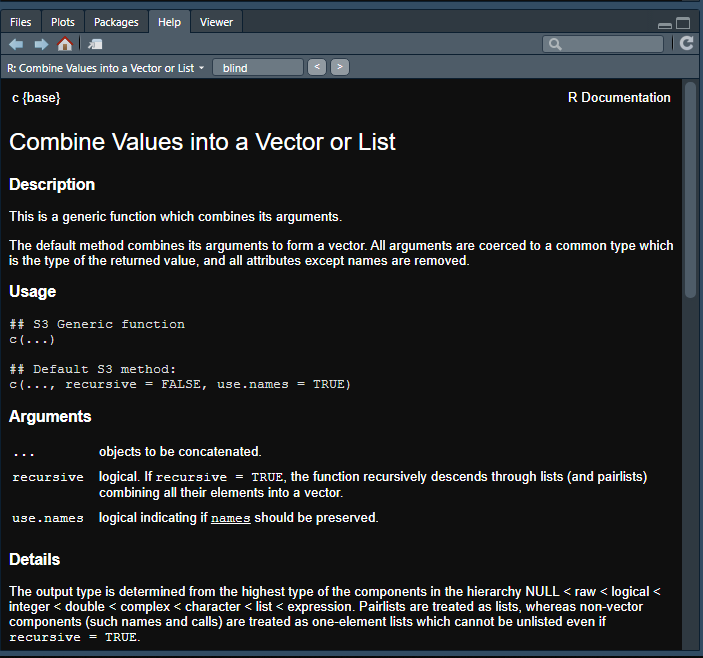
\includegraphics[width=1\linewidth,height=0.45\textheight,]{images/help_page} \end{center}

For \texttt{head()}, all we need to do is tell the function
what data we're looking at. In programming terms, the input
to the function (what we have to include in the parentheses)
is the name of our data object. We'll look at the very
commonly used data called \texttt{mtcars}. \texttt{mtcars}
is one of a small number of data files that are already in R
when you open it. These are included in R just as examples
of data to use when testing our code or teaching people to
use R. Just type \texttt{mtcars} into the console and it
will print out data to the console; there's nothing you need
to do to load the data into R. \texttt{mtcars} has info
about a number of cars with each row being a type of car and
each column being information about the car such as the
miles per gallon it gets and how many gears it has.

We'll use the \texttt{head()} function to print out just the
first 6 rows of the \texttt{mtcars} data.

\begin{Shaded}
\begin{Highlighting}[]
\FunctionTok{head}\NormalTok{(mtcars)}
\CommentTok{\#                    mpg cyl disp  hp drat    wt  qsec vs am}
\CommentTok{\# Mazda RX4         21.0   6  160 110 3.90 2.620 16.46  0  1}
\CommentTok{\# Mazda RX4 Wag     21.0   6  160 110 3.90 2.875 17.02  0  1}
\CommentTok{\# Datsun 710        22.8   4  108  93 3.85 2.320 18.61  1  1}
\CommentTok{\# Hornet 4 Drive    21.4   6  258 110 3.08 3.215 19.44  1  0}
\CommentTok{\# Hornet Sportabout 18.7   8  360 175 3.15 3.440 17.02  0  0}
\CommentTok{\# Valiant           18.1   6  225 105 2.76 3.460 20.22  1  0}
\CommentTok{\#                   gear carb}
\CommentTok{\# Mazda RX4            4    4}
\CommentTok{\# Mazda RX4 Wag        4    4}
\CommentTok{\# Datsun 710           4    1}
\CommentTok{\# Hornet 4 Drive       3    1}
\CommentTok{\# Hornet Sportabout    3    2}
\CommentTok{\# Valiant              3    1}
\end{Highlighting}
\end{Shaded}

Now we have the first 6 rows of every column from the
\texttt{mtcars} data. This is a fairly simple function and
is useful for quickly looking at our data. Many functions
are more complicated than \texttt{head()} and involve
multiple inputs rather than just the single input we had
here. Some functions, for example, let you choose how you
want the function to operate, as it can do so in multiple
ways. Even in \texttt{head()} there's an optional input to
choose how many rows you want it to return, with the default
being 6. Since we didn't choose anything, the function stuck
to the default and returned only 6 rows.

Throughout this book we'll spend a lot of time introducing
functions that other people have made and learning how to
combine the functions together to be able to get our raw
data (e.g.~a CSV file downloaded from a police site) into a
usable format for research (e.g.~cleaned to include only the
rows and columns we need to analyze and in the units we
want). For functions that other people wrote, we need to
tell R that we want to use these functions. We do so by
having R download that person's package. A package is just
the name for a collection of functions in an easily
downloadable format. We can do all of the downloading
through R, so we don't have to go searching for them. There
are two ways to download a package in R: through writing R
code or through a shortcut in RStudio.

Downloading a package through R code uses - like pretty much
everything else in R - a function. This function is
\texttt{install.packages()}, where we put the name of the
package we want in the (). This name also has to be in
quotes since it is an object that is not currently in R.
Let's install the package ``caesar'', which is a simple
package I made that creates a Caesar cipher from some text.
We need to run the code \texttt{install.packages("caesar")}
and be sure to spell ``caesar'' right and put it in quotes.

\begin{Shaded}
\begin{Highlighting}[]
\FunctionTok{install.packages}\NormalTok{(}\StringTok{"caesar"}\NormalTok{)}
\end{Highlighting}
\end{Shaded}

The RStudio shortcut way is to go to the Packages tab and
then click Install on the top left of this tab. This will
open up a window as shown in the following image where you
can enter the name of the package you want. Then click
Install and RStudio will install it for you. Also in this
tab is the Update button, which allows you to update
packages that you have already installed. Since R
programmers generally provide updates to their packages
(usually bug fixes but occasionally new features and new
functions), it's important to update your packages every
several months or so.

\begin{center}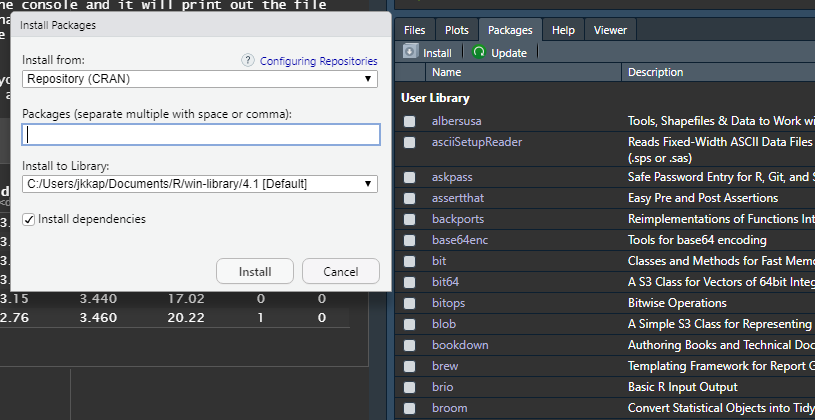
\includegraphics[width=1\linewidth,height=0.45\textheight,]{images/install_packages} \end{center}

Once we have downloaded the package, we need to tell R that
we want to use that package. There are thousands of R
packages and you'll likely have hundreds downloaded before
long (if a package relies on other packages to work it'll
download those too. So even if you install a single package
it may also install other packages necessary for the package
you want). Some packages have functions with the same name
(but they do different things) so using all packages at once
will cause issues since we won't know which functions we're
actually using. So we only want to use the packages we need
for that task. We need a way to tell R that we want to use a
package. We only need to do this once per session - that is,
once before restarting RStudio. The way to do this is to use
the function \texttt{library()}, where we put the package
name in the parentheses. Since the package is something that
has been installed to R, we don't need to have quotes around
the name.

\begin{Shaded}
\begin{Highlighting}[]
\FunctionTok{library}\NormalTok{(caesar)}
\end{Highlighting}
\end{Shaded}

Now we can run the \texttt{caesar()} function and make a
Caesar cipher for that text (it's just a coincidence that
the function name is the same as the package name).

\begin{Shaded}
\begin{Highlighting}[]
\FunctionTok{caesar}\NormalTok{(}\StringTok{"example text"}\NormalTok{)}
\CommentTok{\# [1] "hAdpsohcwhAw"}
\end{Highlighting}
\end{Shaded}

\hypertarget{reading-data-into-r}{%
\section{Reading data into R}\label{reading-data-into-r}}

For many research projects you'll have data produced by some
outside group (e.g.~FBI, local police agencies) and you want
to take that data and put it inside R to work on it. We call
that reading data into R. R is capable of reading a number
of different formats of data, which we will discuss in more
detail in Chapter @ref(reading-and-writing-data). Here, we
will talk about the standard R data file only.

\hypertarget{loading-data-intro}{%
\subsection{Loading data}\label{loading-data-intro}}

As we learned in Section
@ref(setting-the-working-directory), we need to set our
working directory to the folder where the data is. For my
own setup, R is already defaulted to the folder with this
data so I do not need to set a working directory. For those
following along on your own computer, make sure to set your
working directory now.

The \texttt{load()} function lets us load data already in
the R format. These files will end in the extension ``.rda''
or sometimes ``.Rda'' or ``.RData''. Since we are telling R
to load a specific file, we need to have that file name in
quotes and include the file extension ``.rda''. With .rda
data, the object inside the .rda file already has a name so
we don't need to assign a name to the data. With other forms
of data such as .csv files, we will need to do that as we'll
see in Chapter @ref(reading-and-writing-data).

In this example (and elsewhere in this book when I load in
data), I have all of the data in a folder called ``data'' in
my working directory, which is why I have ``data/'' before
the data name. You do not need this as you should have all
of your data directly in your working directory.

\begin{Shaded}
\begin{Highlighting}[]
\FunctionTok{load}\NormalTok{(}\StringTok{"data/ucr2017.rda"}\NormalTok{)}
\end{Highlighting}
\end{Shaded}

\hypertarget{first-steps-to-exploring-data}{%
\section{First steps to exploring
data}\label{first-steps-to-exploring-data}}

The object we loaded is called \texttt{ucr2017}. We'll
explore this data more thoroughly in Chapter @ref(explore),
but for now let's use four simple (and important) functions
to get a sense of what the data holds. To use each of these
functions, we need to write the name of the data set
(without quotes since we don't need quotes for an object
already made in R) inside the ().

\begin{itemize}
\tightlist
\item
  \texttt{head()}
\item
  \texttt{summary()}
\item
  \texttt{plot()}
\item
  \texttt{View()}
\end{itemize}

Note that the first three functions are lowercase while
\texttt{View()} is capitalized. That is simply because older
functions in R were often capitalized while newer ones use
all lowercase letters. R is case sensitive so using
\texttt{view()} will not work.

The \texttt{head()} function prints the first 6 rows of each
column of the data to the console. This is useful to get a
quick glance at the data but has some important drawbacks.
When using data with a large number of columns it can be
quickly overwhelming by printing too much. There may also be
differences in the first 6 rows with other rows. For
example, if the rows are ordered chronologically (as is the
case with most crime data) the first 6 rows will be the most
recent. If data collection methods or the quality of
collection changed over time, these 6 rows won't be
representative of the data.

\begin{Shaded}
\begin{Highlighting}[]
\FunctionTok{head}\NormalTok{(ucr2017)}
\CommentTok{\#       ori year agency\_name  state population actual\_murder}
\CommentTok{\# 1 AK00101 2017   anchorage alaska     296188            27}
\CommentTok{\# 2 AK00102 2017   fairbanks alaska      32937            10}
\CommentTok{\# 3 AK00103 2017      juneau alaska      32344             1}
\CommentTok{\# 4 AK00104 2017   ketchikan alaska       8230             1}
\CommentTok{\# 5 AK00105 2017      kodiak alaska       6198             0}
\CommentTok{\# 6 AK00106 2017        nome alaska       3829             0}
\CommentTok{\#   actual\_rape\_total actual\_robbery\_total}
\CommentTok{\# 1               391                  778}
\CommentTok{\# 2                24                   40}
\CommentTok{\# 3                50                   46}
\CommentTok{\# 4                19                    0}
\CommentTok{\# 5                15                    4}
\CommentTok{\# 6                 7                    0}
\CommentTok{\#   actual\_assault\_aggravated}
\CommentTok{\# 1                      2368}
\CommentTok{\# 2                       131}
\CommentTok{\# 3                       206}
\CommentTok{\# 4                        14}
\CommentTok{\# 5                        41}
\CommentTok{\# 6                        52}
\end{Highlighting}
\end{Shaded}

The \texttt{summary()} function gives a six-number summary
of each numeric or Date column in the data. For other types
of data, such as ``character'' types (which are just columns
with words rather than numbers or dates), it'll say what
type of data it is. We'll cover different types of data in
Chapter @ref(data-types).

The six values it returns for numeric and Date columns are

\begin{itemize}
\tightlist
\item
  The minimum value
\item
  The value at the 1st quartile
\item
  The median value
\item
  The mean value
\item
  The value at the 3rd quartile
\item
  The max value
\end{itemize}

In cases where there are NAs, it will say how many NAs there
are. An NA value is a missing value. Think of it like an
empty cell in an Excel file. NA values will cause issues
when doing math, such as finding the mean of a column, as R
doesn't know how to handle a NA value in these situations,
though \texttt{summary()} automatically excludes NAs when
doing the math operations.

\begin{Shaded}
\begin{Highlighting}[]
\FunctionTok{summary}\NormalTok{(ucr2017)}
\CommentTok{\#      ori                 year      agency\_name       }
\CommentTok{\#  Length:15764       Min.   :2017   Length:15764      }
\CommentTok{\#  Class :character   1st Qu.:2017   Class :character  }
\CommentTok{\#  Mode  :character   Median :2017   Mode  :character  }
\CommentTok{\#                     Mean   :2017                     }
\CommentTok{\#                     3rd Qu.:2017                     }
\CommentTok{\#                     Max.   :2017                     }
\CommentTok{\#     state             population      actual\_murder    }
\CommentTok{\#  Length:15764       Min.   :      0   Min.   :  0.000  }
\CommentTok{\#  Class :character   1st Qu.:    914   1st Qu.:  0.000  }
\CommentTok{\#  Mode  :character   Median :   4460   Median :  0.000  }
\CommentTok{\#                     Mean   :  19872   Mean   :  1.069  }
\CommentTok{\#                     3rd Qu.:  15390   3rd Qu.:  0.000  }
\CommentTok{\#                     Max.   :8616333   Max.   :653.000  }
\CommentTok{\#  actual\_rape\_total  actual\_robbery\_total}
\CommentTok{\#  Min.   :  {-}2.000   Min.   :   {-}1.00    }
\CommentTok{\#  1st Qu.:   0.000   1st Qu.:    0.00    }
\CommentTok{\#  Median :   1.000   Median :    0.00    }
\CommentTok{\#  Mean   :   8.262   Mean   :   19.85    }
\CommentTok{\#  3rd Qu.:   5.000   3rd Qu.:    4.00    }
\CommentTok{\#  Max.   :2455.000   Max.   :13995.00    }
\CommentTok{\#  actual\_assault\_aggravated}
\CommentTok{\#  Min.   :   {-}1.00         }
\CommentTok{\#  1st Qu.:    1.00         }
\CommentTok{\#  Median :    5.00         }
\CommentTok{\#  Mean   :   49.98         }
\CommentTok{\#  3rd Qu.:   21.00         }
\CommentTok{\#  Max.   :29771.00}
\end{Highlighting}
\end{Shaded}

The \texttt{plot()} function allows us to graph our data.
For criminology research we generally want to make
scatterplots to show the relationship between two numeric
variables, time-series graphs to see how a variable (or
variables) change over time, or barplots comparing
categorical variables. Here, we'll make a scatterplot seeing
the relationship between a city's number of murders and
their number of aggravated assaults (assault with a weapon
or that causes serious bodily injury).

To do so we must specify which column is displayed on the
x-axis and which one is displayed on the y-axis. In Section
@ref(select-specific-columns) we'll talk explicitly about
how to select specific columns from our data. For now, all
you need to know is to select a column in which you write
the data set name followed by a dollar sign \texttt{\$},
followed by the column name. Do not include any quotations
or spaces (technically spaces can be included but make it a
bit harder to read and are against conventional style when
writing R code so we'll exclude them). Inside of
\texttt{plot()} we say that ``x = ucr2017\$actual\_murder''
so that column goes on the x-axis and ``y =
ucr2017\$actual\_assault\_aggravated'' so aggravated assault
goes on the y-axis. And that's all it takes to make a simple
graph.

\begin{Shaded}
\begin{Highlighting}[]
\FunctionTok{plot}\NormalTok{(}\AttributeTok{x =}\NormalTok{ ucr2017}\SpecialCharTok{$}\NormalTok{actual\_murder, }\AttributeTok{y =}\NormalTok{ ucr2017}\SpecialCharTok{$}\NormalTok{actual\_assault\_aggravated)}
\end{Highlighting}
\end{Shaded}

\begin{center}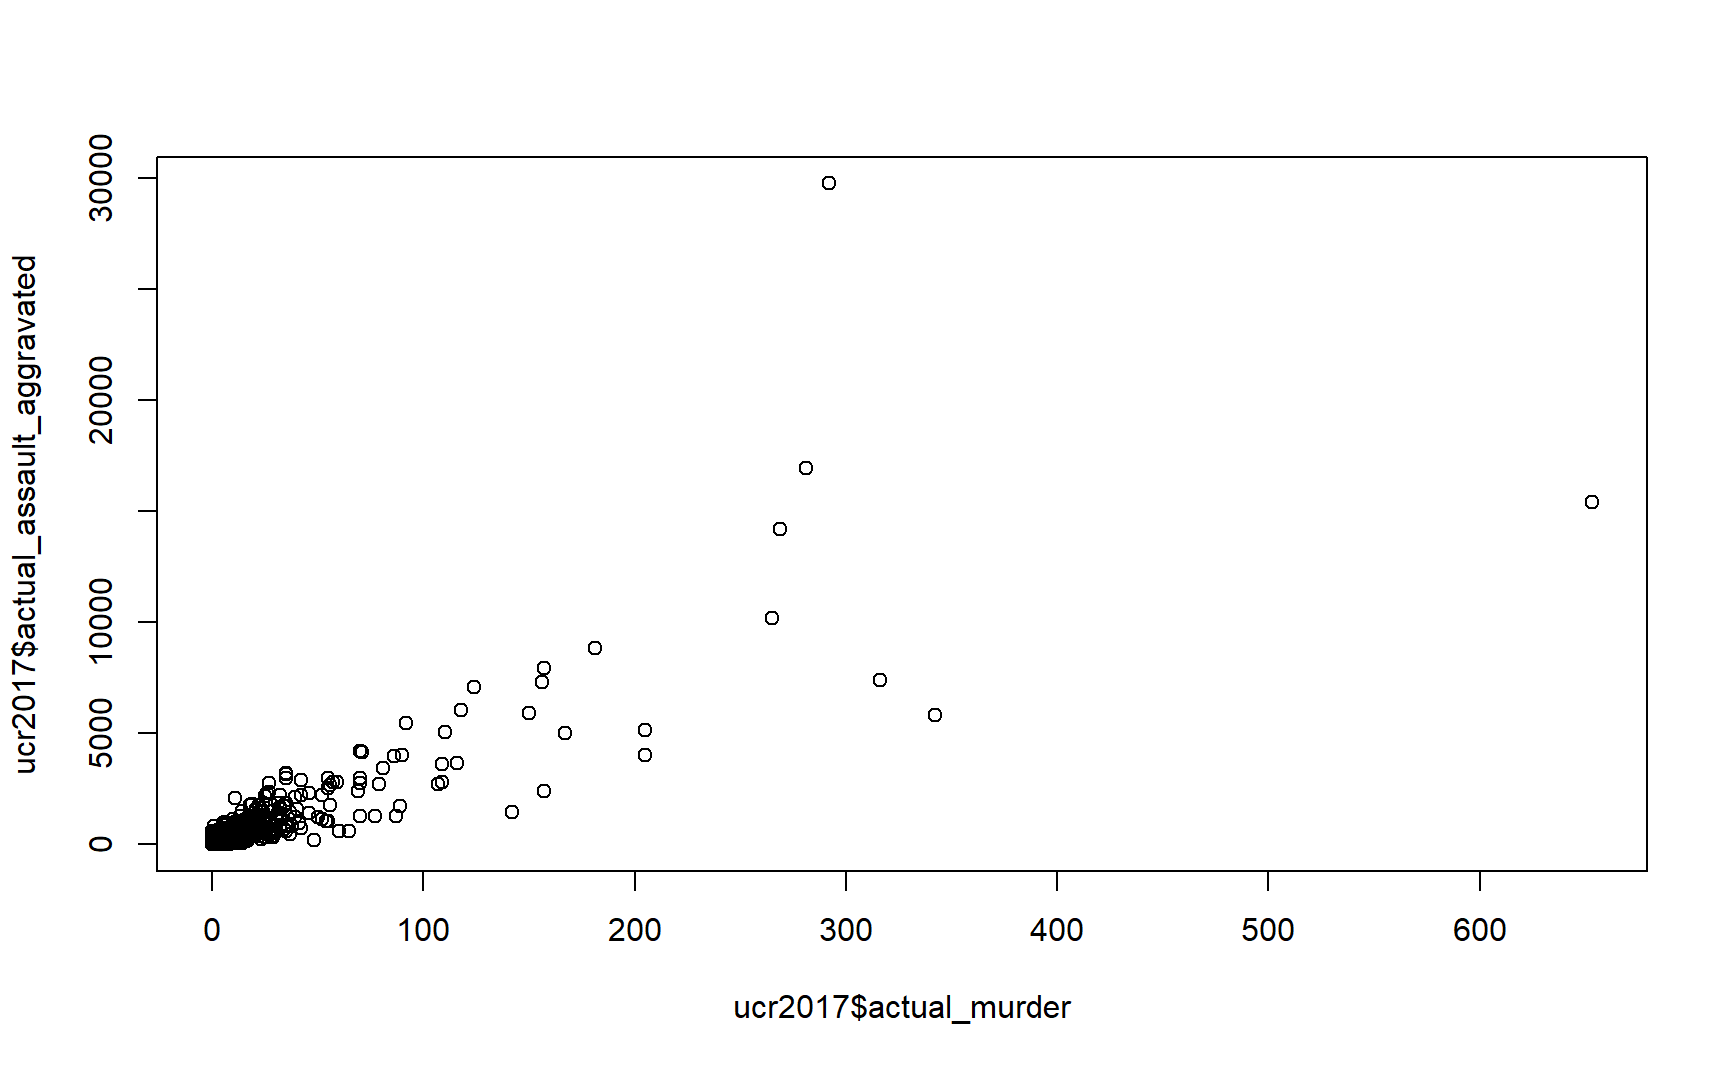
\includegraphics[width=1\linewidth,height=0.45\textheight,]{crimebythenumbers_files/figure-latex/unnamed-chunk-40-1} \end{center}

Finally, \texttt{View()} opens essentially an Excel file of
the data set you put inside the (). This allows you to look
at the data as if it were in Excel (though you can't edit
the data at all here) and is a good way to start to
understand the data.

\begin{Shaded}
\begin{Highlighting}[]
\FunctionTok{View}\NormalTok{(ucr2017)}
\end{Highlighting}
\end{Shaded}

\hypertarget{data-types}{%
\chapter{Data types and structures}\label{data-types}}

\hypertarget{section-data-types}{%
\section{Data types}\label{section-data-types}}

When you read a sentence like ``two plus two'' you know the
answer is four. R doesn't know that. This is because R takes
things very literally. It will read ``two'' as a word, not
as a number. For R to understand numbers you need to specify
that you're talking about numbers, and not just words. Let's
look at an example, making two variables which each have the
value of ``2.''

\begin{Shaded}
\begin{Highlighting}[]
\NormalTok{a }\OtherTok{\textless{}{-}} \StringTok{"2"}
\NormalTok{b }\OtherTok{\textless{}{-}} \StringTok{"2"}
\end{Highlighting}
\end{Shaded}

We now have a and b that are equal to ``2'' (in quotes!).
Let's try to add them.

\begin{Shaded}
\begin{Highlighting}[]
\NormalTok{a }\SpecialCharTok{+}\NormalTok{ b}
\CommentTok{\# Error in a + b: non{-}numeric argument to binary operator}
\end{Highlighting}
\end{Shaded}

We get an error that is a technical way of saying that we
did math on something that isn't a number. That's because we
made a and b get ``2'' with quotes around it, which R
interpreted as a word, not as a number. If we change a and b
to 2 (without quotes), then R will know that the 2 is a
number, and will do math on it.

\begin{Shaded}
\begin{Highlighting}[]
\NormalTok{a }\OtherTok{\textless{}{-}} \DecValTok{2}
\NormalTok{b }\OtherTok{\textless{}{-}} \DecValTok{2}
\NormalTok{a }\SpecialCharTok{+}\NormalTok{ b}
\CommentTok{\# [1] 4}
\end{Highlighting}
\end{Shaded}

This may seem like a pretty simple concept but is
fundamental to how R works, and can trip up new and
experienced programmers alike. R trusts you. It only knows
what you tell it. If you tell it that something is a word
(by including quotes), it will treat it as a word, even if
it looks to you like a number. So we must be very precise
about what code we write, as R won't (for the most part) fix
our mistakes - though it will give us an error if we try to
do something it doesn't like, like add two words.

\hypertarget{numeric-character-and-logical-boolean}{%
\section{Numeric, character, and logical
(boolean)}\label{numeric-character-and-logical-boolean}}

There are three main data types that are important to know
for using R to do research: numeric, character, and logical.

A numeric type is a number, and this includes both integers
like 2 and decimals like 2.5. You can tell something is
numeric if it is a number and there are no quotes around it.
2 is a number, ``2'' is not. For real data this will likely
be something like the age of an individual or the number of
crimes in a city. We want it as numeric type because we can
do math on numbers. For example, we can find the average age
of victims of crimes, or the median number of crimes in a
city each week. This won't work unless R knows that these
values are numbers.

A character is just a word or a set of words. If it is in
quotes it's a character. Other programming languages
generally call this a string instead of a character, but
they mean the same thing. Pretty much anything that you'd
write in English class fits in here.

Finally, a logical data type is just a true or false value,
though in R it must be written all in capital letters: TRUE
or FALSE. This is also referred to as a Boolean value.
Booleans or logical data are useful when comparing two
things. For example, we can see if 2 is equal to 3.

\begin{Shaded}
\begin{Highlighting}[]
\DecValTok{2} \SpecialCharTok{==} \DecValTok{3}
\CommentTok{\# [1] FALSE}
\end{Highlighting}
\end{Shaded}

It's not, so R returned FALSE (the == just compares the
thing on the left to the thing on the right). This is very
useful when we want to keep only certain rows in our data.
For example, if we had data on multiple years of crime and
we only wanted to keep a single year (let's say 2020), we
could tell R to keep only rows where the year equals 2020 -
where it is TRUE that that row's year column is equal to
what year we want. We'll cover this in great detail in
Chapter @ref(subsetting-intro).

While you could try to figure out what type of data
something is just by looking at it, R has a number of
functions to check for you. We'll look at a few general
functions that tell you the type of data something is, and
then ones that check if the data is a specific type.

First, the \texttt{is()} function tells you all of the types
of data something is - and a value can actually have
multiple types. While it can't be both, for example, numeric
and character, it can have other data types that we'll look
at in the next section. First, let's look at what
\texttt{is()} returns (prints out to the console) for a few
simple examples.

\begin{Shaded}
\begin{Highlighting}[]
\FunctionTok{is}\NormalTok{(}\DecValTok{2}\NormalTok{)}
\CommentTok{\# [1] "numeric" "vector"}
\end{Highlighting}
\end{Shaded}

Checking what 2 is tells us that it is both a ``numeric''
type and a ``vector'' type.

\begin{Shaded}
\begin{Highlighting}[]
\FunctionTok{is}\NormalTok{(}\StringTok{"2"}\NormalTok{)}
\CommentTok{\# [1] "character"           "vector"             }
\CommentTok{\# [3] "data.frameRowLabels" "SuperClassMethod"}
\end{Highlighting}
\end{Shaded}

Checking ``2'' (in quotes), gives us four different types of
data for this value: ``character'', ``vector'',
``data.frameRowLabels'', and ``SuperClassMethod''. You can
ignore the last two types, we just are interested in that it
is a ``character'' type and, like the type of 2, is a
``vector''.

\begin{Shaded}
\begin{Highlighting}[]
\FunctionTok{is}\NormalTok{(}\ConstantTok{TRUE}\NormalTok{)}
\CommentTok{\# [1] "logical" "vector"}
\end{Highlighting}
\end{Shaded}

Finally, checking what TRUE is returns both ``logical'' and
``vector''. We expected logical since TRUE is a logical
type. Again, we see that it is also a vector type. TRUE has
to be both in capital letters and not be in quotes. If we
write it in quotes then R will think it is a character, and
if we have it lowercase and without quotes R will think that
it is an object (such as something we make using
\texttt{\textless{}-} and not a Boolean).

\begin{Shaded}
\begin{Highlighting}[]
\FunctionTok{is}\NormalTok{(}\StringTok{"TRUE"}\NormalTok{)}
\CommentTok{\# [1] "character"           "vector"             }
\CommentTok{\# [3] "data.frameRowLabels" "SuperClassMethod"}
\end{Highlighting}
\end{Shaded}

\begin{Shaded}
\begin{Highlighting}[]
\FunctionTok{is}\NormalTok{(true)}
\CommentTok{\# Error in is(true): object \textquotesingle{}true\textquotesingle{} not found}
\end{Highlighting}
\end{Shaded}

All three of the values we checked say that they are a
``vector'' type. We'll cover vectors in the next section,
but for now let's see one other function that tells us the
type of data something is. If we use \texttt{class()}
instead of \texttt{is()} we'll get just the first value
returned in the types of data that we input.

\begin{Shaded}
\begin{Highlighting}[]
\FunctionTok{class}\NormalTok{(}\DecValTok{2}\NormalTok{)}
\CommentTok{\# [1] "numeric"}
\FunctionTok{class}\NormalTok{(}\StringTok{"2"}\NormalTok{)}
\CommentTok{\# [1] "character"}
\FunctionTok{class}\NormalTok{(}\ConstantTok{TRUE}\NormalTok{)}
\CommentTok{\# [1] "logical"}
\end{Highlighting}
\end{Shaded}

In a lot of cases we'll want to check if some data is a
specific type. For example, we might want to check that the
year column of a data set is numeric, rather than say
character. We do this with three functions, each of which
checks that the data input (the data put in the parentheses
of the function) is that type of data or not. These
functions are: \texttt{is.numeric()},
\texttt{is.character()}, and \texttt{is.logical()}.

Running any of these functions will actually return a
logical value, either TRUE or FALSE telling us if the value
inputted is that type.

\begin{Shaded}
\begin{Highlighting}[]
\FunctionTok{is.numeric}\NormalTok{(}\DecValTok{2}\NormalTok{)}
\CommentTok{\# [1] TRUE}
\FunctionTok{is.character}\NormalTok{(}\StringTok{"2"}\NormalTok{)}
\CommentTok{\# [1] TRUE}
\FunctionTok{is.character}\NormalTok{(}\DecValTok{2}\NormalTok{)}
\CommentTok{\# [1] FALSE}
\FunctionTok{is.logical}\NormalTok{(}\ConstantTok{TRUE}\NormalTok{)}
\CommentTok{\# [1] TRUE}
\end{Highlighting}
\end{Shaded}

So far we've just been checking the value of a single thing:
a single number, a single character/string, or a single
logical/Boolean value. In practice almost everything we do
will be on a column of a data set. These functions still
work in the exact same way. We input the column (using the
data\$column syntax discussed in Chapter @ref(intro-to-r) to
specify which data set we want and specifically which column
in that data set) and the function will behave just like it
did above. That's because each column can only be a single
type of data; if the column is numeric, all values will be
numeric; if the column is character, all values in that
column are character; if the column is logical, every value
in that column is also logical.

Let's use the UCR data from 2017 that was introduced in
Chapter @ref(intro-to-r). Remember that the data must be in
your working directory to load it. And here I have ``data/''
before the data name because the data is in a folder called
``data'' in my working directory. For more on working
directories, please see Section
@ref(setting-the-working-directory).

\begin{Shaded}
\begin{Highlighting}[]
\FunctionTok{load}\NormalTok{(}\StringTok{"data/ucr2017.rda"}\NormalTok{)}
\end{Highlighting}
\end{Shaded}

We need to know the column names before using them, so we
can use the \texttt{names()} function to get a list of all
of the column names (the \texttt{colnames()} function does
the same thing).

\begin{Shaded}
\begin{Highlighting}[]
\FunctionTok{names}\NormalTok{(ucr2017)}
\CommentTok{\# [1] "ori"                       "year"                     }
\CommentTok{\# [3] "agency\_name"               "state"                    }
\CommentTok{\# [5] "population"                "actual\_murder"            }
\CommentTok{\# [7] "actual\_rape\_total"         "actual\_robbery\_total"     }
\CommentTok{\# [9] "actual\_assault\_aggravated"}
\end{Highlighting}
\end{Shaded}

Now we can check the types of some of the columns. Let's
check the year column as an example. A year is a number so
we may expect it to be numeric, but there's technically
nothing stopping that data from being character type. It
can't be logical type because then instead of a year value
it'd just be TRUE or FALSE, which is certainly not what a
year is.

\begin{Shaded}
\begin{Highlighting}[]
\FunctionTok{is}\NormalTok{(ucr2017}\SpecialCharTok{$}\NormalTok{year)}
\CommentTok{\# [1] "numeric" "vector"}
\end{Highlighting}
\end{Shaded}

And we can use \texttt{is.numeric()} as another way to see
if this column is numeric.

\begin{Shaded}
\begin{Highlighting}[]
\FunctionTok{is.numeric}\NormalTok{(ucr2017}\SpecialCharTok{$}\NormalTok{year)}
\CommentTok{\# [1] TRUE}
\end{Highlighting}
\end{Shaded}

\hypertarget{data-structures}{%
\section{Data structures}\label{data-structures}}

We'll look in detail about two important data structures -
vectors and data.frames - and then talk briefly about two
other structures that are not that important in this book,
but are nonetheless good to know that they exist. So far
we've just been looking at either a single value, such as
\texttt{a\ \textless{}-\ 1} or more complicated structures
such as the ucr2017 data set, which is called a data.frame -
R's version of an Excel file. Data structures each operate a
little differently from each other so it's good to
understand what they are and how they work. We'll cover much
more of how they work in Chapter @ref(subsetting-intro),
which covers how to subset data - which is just how to keep
only certain values (such as specific rows or columns) in
the data.

\hypertarget{vectors}{%
\subsection{Vectors (collections of
``things'')}\label{vectors}}

The first data structure we'll discuss is a vector. A vector
is a collection of same type (numeric, character, logical,
Date) values in a single object. When we made ``a'' in
Chapter @ref(intro-to-r), we assigned it only a single
value, such as \texttt{a\ \textless{}-\ 1}. Usually we'll
want to have a group of values - such as a set of years or a
group of crime types - rather than just a single value. We
can do this by using the same assignment method as
\texttt{a\ \textless{}-\ 1} but put all of the values we
want to assign to a into the function \texttt{c()} and
separate each value by a comma. The \texttt{c()} function
\textbf{c}ombines each value together into a single vector.

Now, technically a single value, such as our object called
``a'' which now equals 1, is still a vector. In this case
it'd be a vector of length 1, since there is only one value
in it. But when we generally talk about vectors there are
multiple elements in it.

Here's an example of making the object a be a vector with
three values: 1, 2, and 3 (in that order).

\begin{Shaded}
\begin{Highlighting}[]
\NormalTok{a }\OtherTok{\textless{}{-}} \FunctionTok{c}\NormalTok{(}\DecValTok{1}\NormalTok{, }\DecValTok{2}\NormalTok{, }\DecValTok{3}\NormalTok{)}
\end{Highlighting}
\end{Shaded}

It is absolutely crucial to have the \texttt{c()} function,
otherwise we'd get an error from R.

\begin{Shaded}
\begin{Highlighting}[]
\NormalTok{a }\OtherTok{\textless{}{-}}\NormalTok{ (}\DecValTok{1}\NormalTok{, }\DecValTok{2}\NormalTok{, }\DecValTok{3}\NormalTok{)}
\CommentTok{\# Error: \textless{}text\textgreater{}:1:8: unexpected \textquotesingle{},\textquotesingle{}}
\CommentTok{\# 1: a \textless{}{-} (1,}
\CommentTok{\#            \^{}}
\end{Highlighting}
\end{Shaded}

It is likewise crucial to have a comma separating every
single separate value.

\begin{Shaded}
\begin{Highlighting}[]
\NormalTok{a }\OtherTok{\textless{}{-}} \FunctionTok{c}\NormalTok{(}\DecValTok{1} \DecValTok{2} \DecValTok{3}\NormalTok{)}
\CommentTok{\# Error: \textless{}text\textgreater{}:1:10: unexpected numeric constant}
\CommentTok{\# 1: a \textless{}{-} c(1 2}
\CommentTok{\#              \^{}}
\end{Highlighting}
\end{Shaded}

The terminology for talking about values in a vector is that
each value is called an ``element,'' and we identify them by
the number they are, in order from start to finish. So here
we have 1, 2, and 3, and we can say that the first element
is 1, the second element is 2, the third element is 3.

If we assigned a to b (\texttt{b\ \textless{}-\ a}) we don't
need to use the \texttt{c()} again. a is already a vector so
if we assign its value to something, that carries over the
vector. The \texttt{c()} is only necessary when first
creating the vector.

Note that vectors take values that are the same type, so all
values included must be the same type, such as a number or a
string. If they aren't the same type, R will automatically
convert it to the same type.

\begin{Shaded}
\begin{Highlighting}[]
\FunctionTok{c}\NormalTok{(}\StringTok{"cat"}\NormalTok{, }\StringTok{"dog"}\NormalTok{, }\DecValTok{2}\NormalTok{)}
\CommentTok{\# [1] "cat" "dog" "2"}
\end{Highlighting}
\end{Shaded}

Above we made a vector with the values ``cat'', ``dog'' and
2 (without quotes) and it added quotes to the 2. Since
everything must be the same type, R automatically converted
the 2 to a string of ``2''.

\hypertarget{dataframes}{%
\subsection{Data.frames}\label{dataframes}}

Nearly everything you do in this book and in research will
be through data.frames. A data.frame is basically R's
version of an Excel file. More precisely, a data.frame is a
collection of equal-length vectors. Each column in a
data.frame is actually a vector. They must all be equal
length so every column has the same number of rows. You
can't have, for example, a data.frame with 10 rows of data
for the city column and only 8 rows for the year column. It
must be 10 for each. Since vectors can only be a single
type, each row in a particular column in a data.frame must
be the same type, though different columns can be different
types. This is how we can have, for example, our ucr2017
data.frame, which has both numeric and character type
columns.

In this book I'll refer to data.frames by keeping it all
lower case and with a dot between the words. This is just
because the function to make one is \texttt{data.frame()},
and writing it this way is the normal convention. But
writing it as a data frame is also fine. In nearly all cases
we'll be using data that is loaded into R and is already in
the structure of a data.frame (usually these will be Excel
files or R data files like an .rda or .rds file).

If we wanted to create our own data.frame we would use the
\texttt{data.frame()}, function and the input would be
vectors, which will become our columns. Let's make a simple
one. If the vector is already created then R would
automatically take the name of that vector object as the
column name, otherwise we could name it ourselves

\begin{Shaded}
\begin{Highlighting}[]
\NormalTok{example }\OtherTok{\textless{}{-}} \FunctionTok{data.frame}\NormalTok{(}
  \AttributeTok{column\_1 =} \FunctionTok{c}\NormalTok{(}\DecValTok{1}\NormalTok{, }\DecValTok{3}\NormalTok{, }\DecValTok{5}\NormalTok{, }\DecValTok{7}\NormalTok{, }\DecValTok{9}\NormalTok{),}
  \AttributeTok{column2 =} \FunctionTok{c}\NormalTok{(}
    \StringTok{"hello"}\NormalTok{,}
    \StringTok{"darkness"}\NormalTok{,}
    \StringTok{"my"}\NormalTok{,}
    \StringTok{"old"}\NormalTok{,}
    \StringTok{"friend"}
\NormalTok{  )}
\NormalTok{)}
\NormalTok{example}
\CommentTok{\#   column\_1  column2}
\CommentTok{\# 1        1    hello}
\CommentTok{\# 2        3 darkness}
\CommentTok{\# 3        5       my}
\CommentTok{\# 4        7      old}
\CommentTok{\# 5        9   friend}
\end{Highlighting}
\end{Shaded}

Now we have a new data.frame called example, which has two
columns and five rows. We named the columns ourselves, and
in this case we don't need to put the column name in quotes,
though doing so would give the same result. Here we're
saying that the column ``column\_1'' is equal to the vector
\texttt{c(1,\ 3,\ 5,\ 7,\ 9)} and ``column\_2'' is equal to
the vector
\texttt{c("hello",\ "darkness",\ "my",\ "old",\ "friend")}.
We're essentially creating an object inside of the
\texttt{data.frame()} function but in this case we need to
use the equal sign and not the \texttt{\textless{}-} because
R doesn't allow the use of \texttt{\textless{}-} inside of a
function.

If we forget to name the columns, and our vectors aren't
already created with their own name, R will create a name
based on the values in that vector. As shown below, this
looks really bad so make sure to always name your columns.

\begin{Shaded}
\begin{Highlighting}[]
\NormalTok{example }\OtherTok{\textless{}{-}} \FunctionTok{data.frame}\NormalTok{(}
  \FunctionTok{c}\NormalTok{(}\DecValTok{1}\NormalTok{, }\DecValTok{3}\NormalTok{, }\DecValTok{5}\NormalTok{, }\DecValTok{7}\NormalTok{, }\DecValTok{9}\NormalTok{),}
  \FunctionTok{c}\NormalTok{(}
    \StringTok{"hello"}\NormalTok{,}
    \StringTok{"darkness"}\NormalTok{,}
    \StringTok{"my"}\NormalTok{,}
    \StringTok{"old"}\NormalTok{,}
    \StringTok{"friend"}
\NormalTok{  )}
\NormalTok{)}
\NormalTok{example}
\CommentTok{\#   c.1..3..5..7..9.}
\CommentTok{\# 1                1}
\CommentTok{\# 2                3}
\CommentTok{\# 3                5}
\CommentTok{\# 4                7}
\CommentTok{\# 5                9}
\CommentTok{\#   c..hello....darkness....my....old....friend..}
\CommentTok{\# 1                                         hello}
\CommentTok{\# 2                                      darkness}
\CommentTok{\# 3                                            my}
\CommentTok{\# 4                                           old}
\CommentTok{\# 5                                        friend}
\end{Highlighting}
\end{Shaded}

If the vectors are already made then we won't have an issue.
R will default to the vector name, but we can override that
if we want.

\begin{Shaded}
\begin{Highlighting}[]
\NormalTok{column\_1 }\OtherTok{\textless{}{-}} \FunctionTok{c}\NormalTok{(}\DecValTok{1}\NormalTok{, }\DecValTok{3}\NormalTok{, }\DecValTok{5}\NormalTok{, }\DecValTok{7}\NormalTok{, }\DecValTok{9}\NormalTok{)}
\NormalTok{column2 }\OtherTok{\textless{}{-}} \FunctionTok{c}\NormalTok{(}\StringTok{"hello"}\NormalTok{, }\StringTok{"darkness"}\NormalTok{, }\StringTok{"my"}\NormalTok{, }\StringTok{"old"}\NormalTok{, }\StringTok{"friend"}\NormalTok{)}
\NormalTok{example }\OtherTok{\textless{}{-}} \FunctionTok{data.frame}\NormalTok{(column\_1,}
  \AttributeTok{overridden\_name =}\NormalTok{ column2}
\NormalTok{)}
\NormalTok{example}
\CommentTok{\#   column\_1 overridden\_name}
\CommentTok{\# 1        1           hello}
\CommentTok{\# 2        3        darkness}
\CommentTok{\# 3        5              my}
\CommentTok{\# 4        7             old}
\CommentTok{\# 5        9          friend}
\end{Highlighting}
\end{Shaded}

As with other objects, we can use the \texttt{is()} function
to see what type it is. If we use \texttt{is()} on our
example object, it'll tell us that it is a data.frame.

\begin{Shaded}
\begin{Highlighting}[]
\FunctionTok{is}\NormalTok{(example)}
\CommentTok{\# [1] "data.frame" "list"       "oldClass"   "vector"}
\end{Highlighting}
\end{Shaded}

We also often will want to know how many columns and rows a
data.frame has. For finding the number of rows we use the
function \texttt{nrow()}, and for finding the number of
columns we'll use the \texttt{ncol()} function.\footnote{We
  could also use the \texttt{dim()}, function which tells
  the dimensions of the data.frame. The dimensions are the
  rows and columns in the data.frame so \texttt{dim()} tell
  us the results of both \texttt{nrow()} and \texttt{ncol()}
  at the same time. This function returns a vector showing
  first the number of rows and then the number of columns.
  But I find it easier to simply ask for the number of rows
  or columns separately, and to not deal with the result,
  which has two values.} In each the ``n'' part of the
function just stands for number. So \texttt{nrow()} is
number of rows. For each we put our data.frame object in the
parentheses (without quotes since it is something already
loaded in R), and it will return the number of rows/columns.

\begin{Shaded}
\begin{Highlighting}[]
\FunctionTok{nrow}\NormalTok{(example)}
\CommentTok{\# [1] 5}
\end{Highlighting}
\end{Shaded}

\begin{Shaded}
\begin{Highlighting}[]
\FunctionTok{ncol}\NormalTok{(example)}
\CommentTok{\# [1] 2}
\end{Highlighting}
\end{Shaded}

Alternatively, we could have looked in the Environment tab
which shows us the number of rows and columns of each
data.frame that is loaded to R. For example, ucr2017 says it
has ``15764 obs. of 9 variables''. This just means there are
15,764 rows and 9 variables. A variable in this context is
just another way to say a column. However, you'll
occasionally want to find the exact number of rows and
columns, and as you'll often delete certain rows and columns
from your data this can change throughout your code. So
being able to use \texttt{nrow()} and \texttt{ncol()} is
easier than repeatedly checking the Environment tab.

You may encounter something called a data.table or a tibble.
These are two popular variations of data.frames that operate
much the same way as data.frames but with some different
features. We'll use tibbles in this book so will discuss
their features when we use them.

\hypertarget{other-data-structures}{%
\subsection{Other data
structures}\label{other-data-structures}}

There are two other data structures that I'll mention only
so you have heard of them and can look up more information
on them if you'd like. However, these are not \emph{that}
important to know about for the purpose of this book. Some
of these structures may come up in rare cases when you're
programming, so it's important to know that they exist.

The first data structure is a list. A list is essentially a
vector but where different values can be different types.
Lists are actually very powerful data structures and ones
that you'll encounter a lot when using R, but are almost
entirely on the backend of R so not things you'll actually
deal with much. For example, all data.frames are actually
lists. And more specifically, they are a list of vectors.
Lists can come in handy because they can store different
types of data structures. A single list can, for example,
have a number, a vector, a matrix (discussed below), and an
entire data.frame inside. Lists can even have other lists
inside of them. Let's look at an example of this.

\begin{Shaded}
\begin{Highlighting}[]
\NormalTok{list\_example }\OtherTok{\textless{}{-}} \FunctionTok{list}\NormalTok{(}
  \StringTok{"hello"}\NormalTok{,}
  \DecValTok{1}\SpecialCharTok{:}\DecValTok{5}\NormalTok{,}
  \DecValTok{6}\SpecialCharTok{:}\DecValTok{10}\NormalTok{,}
  \FunctionTok{list}\NormalTok{(}\FunctionTok{c}\NormalTok{(}\DecValTok{33}\NormalTok{, }\DecValTok{66}\NormalTok{, }\DecValTok{99}\NormalTok{)),}
  \FunctionTok{head}\NormalTok{(mtcars)}
\NormalTok{)}
\FunctionTok{head}\NormalTok{(list\_example)}
\CommentTok{\# [[1]]}
\CommentTok{\# [1] "hello"}
\CommentTok{\# }
\CommentTok{\# [[2]]}
\CommentTok{\# [1] 1 2 3 4 5}
\CommentTok{\# }
\CommentTok{\# [[3]]}
\CommentTok{\# [1]  6  7  8  9 10}
\CommentTok{\# }
\CommentTok{\# [[4]]}
\CommentTok{\# [[4]][[1]]}
\CommentTok{\# [1] 33 66 99}
\CommentTok{\# }
\CommentTok{\# }
\CommentTok{\# [[5]]}
\CommentTok{\#                    mpg cyl disp  hp drat    wt  qsec vs am}
\CommentTok{\# Mazda RX4         21.0   6  160 110 3.90 2.620 16.46  0  1}
\CommentTok{\# Mazda RX4 Wag     21.0   6  160 110 3.90 2.875 17.02  0  1}
\CommentTok{\# Datsun 710        22.8   4  108  93 3.85 2.320 18.61  1  1}
\CommentTok{\# Hornet 4 Drive    21.4   6  258 110 3.08 3.215 19.44  1  0}
\CommentTok{\# Hornet Sportabout 18.7   8  360 175 3.15 3.440 17.02  0  0}
\CommentTok{\# Valiant           18.1   6  225 105 2.76 3.460 20.22  1  0}
\CommentTok{\#                   gear carb}
\CommentTok{\# Mazda RX4            4    4}
\CommentTok{\# Mazda RX4 Wag        4    4}
\CommentTok{\# Datsun 710           4    1}
\CommentTok{\# Hornet 4 Drive       3    1}
\CommentTok{\# Hornet Sportabout    3    2}
\CommentTok{\# Valiant              3    1}
\end{Highlighting}
\end{Shaded}

The list that I called list\_example contains six different
elements in it: a character, two numeric vectors, a list of
a numeric vector, and the first six rows of the mtcars
data.frame. Lists can be useful when storing many different
objects at once, but as they are not used too often for
research-related programming I'll say no more of them.

The other type of data structure is a matrix. A matrix is a
two-dimensional object where every value is the same type.
Think of a data.frame but each column has to be the same
type. Below is an example of a matrix with values 1 through
50 and with five columns and five rows. Every value here is
a number.

\begin{Shaded}
\begin{Highlighting}[]
\FunctionTok{matrix}\NormalTok{(}\DecValTok{1}\SpecialCharTok{:}\DecValTok{50}\NormalTok{, }\AttributeTok{nrow =} \DecValTok{5}\NormalTok{, }\AttributeTok{ncol =} \DecValTok{5}\NormalTok{)}
\CommentTok{\#      [,1] [,2] [,3] [,4] [,5]}
\CommentTok{\# [1,]    1    6   11   16   21}
\CommentTok{\# [2,]    2    7   12   17   22}
\CommentTok{\# [3,]    3    8   13   18   23}
\CommentTok{\# [4,]    4    9   14   19   24}
\CommentTok{\# [5,]    5   10   15   20   25}
\end{Highlighting}
\end{Shaded}

If I change it to have the first value be ``1'' (in quotes
so it is a character) and the others be the numbers 2
through 50, the matrix will automatically convert everything
to a character type. So it will remain having everything be
the same type, but now everything is a character.

\begin{Shaded}
\begin{Highlighting}[]
\FunctionTok{matrix}\NormalTok{(}\FunctionTok{c}\NormalTok{(}\StringTok{"1"}\NormalTok{, }\DecValTok{2}\SpecialCharTok{:}\DecValTok{50}\NormalTok{), }\AttributeTok{nrow =} \DecValTok{5}\NormalTok{, }\AttributeTok{ncol =} \DecValTok{5}\NormalTok{)}
\CommentTok{\#      [,1] [,2] [,3] [,4] [,5]}
\CommentTok{\# [1,] "1"  "6"  "11" "16" "21"}
\CommentTok{\# [2,] "2"  "7"  "12" "17" "22"}
\CommentTok{\# [3,] "3"  "8"  "13" "18" "23"}
\CommentTok{\# [4,] "4"  "9"  "14" "19" "24"}
\CommentTok{\# [5,] "5"  "10" "15" "20" "25"}
\end{Highlighting}
\end{Shaded}

\hypertarget{reading-and-writing-data}{%
\chapter{Reading and writing
data}\label{reading-and-writing-data}}

For this chapter you'll need the following files, which are
available for download
\href{https://github.com/jacobkap/r4crimz/tree/master/data}{here}:
fatal-police-shootings-data.csv,
fatal-police-shootings-data.dta,
fatal-police-shootings-data.sas,
fatal-police-shootings-data.sav, sqf-2019.xlsx,
sf\_neighborhoods\_suicide.rda, and shr\_1976\_2020.rds.

So far in these lessons we've used data from a number of
sources, but which came as .rda or .rds files, which are the
standard R data formats. Many data sets, particularly older
government data, will not come as .rda or .rds files but
rather as Excel, Stata, SAS, SPSS, or fixed-width ASCII
files. In this brief lesson, we'll cover how to read these
formats into R as well as how to save data into these
formats. Since many criminologists do not use R, it is
important to be able to save the data in the language they
use to be able to collaborate with them.

In this lesson we'll load and save multiple files into R as
examples of how R can handle data that is used in many
different software programs.

When loading data into R remember that your data must be in
your current working directory or R won't be able to read
it. For a refresher on working directories please see
Section @ref(setting-the-working-directory). In these
examples I have my data in a folder called ``data'' that is
in my working directory, which is why I use ``data/'' when
naming the file. You do not need to include ``data/'' when
loading in data on your computer.

\hypertarget{reading-data-into-r-1}{%
\section{Reading data into R}\label{reading-data-into-r-1}}

\hypertarget{r}{%
\subsection{R}\label{r}}

\hypertarget{rda-and-.rdata-files}{%
\subsubsection{.rda and .rdata
files}\label{rda-and-.rdata-files}}

As we've seen earlier, to read in data with a .rda or .rdata
extension you use the function \texttt{load()} with the file
name (including the extension) in quotation marks inside of
the parentheses. This loads the data into R and calls the
object the name it was when it was saved. Therefore we do
not need to give it a name ourselves.

Below, we're loading the ``sf\_neighborhoods\_suicide.rda''
file, and it creates an object in R (which we can look at in
the Environment tab) called ``sf\_neighborhoods\_suicide''.
It has the same name only because when I originally saved
the file I saved it using the same name as it was called in
R. But in practice I could have called it whatever I wanted.
So it being the same name is convenient, as it is clear what
the data is, but not necessary.

\begin{Shaded}
\begin{Highlighting}[]
\FunctionTok{load}\NormalTok{(}\StringTok{"data/sf\_neighborhoods\_suicide.rda"}\NormalTok{)}
\end{Highlighting}
\end{Shaded}

\hypertarget{rds-files}{%
\subsubsection{.rds files}\label{rds-files}}

For each of the other types of data we'll need to assign a
name to the data we're reading in. Whereas we've done
\texttt{x\ \textless{}-\ 2} to say \emph{x} gets the value
of 2, now we'd do \texttt{x\ \textless{}-\ DATA} where DATA
is the way to load in the data, and \emph{x} will get the
entire data set that is read in.

This includes the other kind of R data file, the .rds file.
Here, we must explicitly name the data - there is no name by
default like in a .rda or a .rdata file. We can load .rds
files into R using the \texttt{readRDS()}, which is built
into R so we don't need any package to use it. Like in
\texttt{load()}, we just put the name of the file (in
quotes) in the parentheses. Here we're naming it
``rds\_example,'' but we can name it whatever we like.

\begin{Shaded}
\begin{Highlighting}[]
\NormalTok{rds\_example }\OtherTok{\textless{}{-}} \FunctionTok{readRDS}\NormalTok{(}\StringTok{"data/shr\_1976\_2020.rds"}\NormalTok{)}
\end{Highlighting}
\end{Shaded}

\hypertarget{excel}{%
\subsection{Excel}\label{excel}}

To read in Excel files that end in .csv, we can use the
function \texttt{read\_csv()} from the package
\texttt{readr} (the function \texttt{read.csv()} is included
in R by default so it doesn't require any packages but is
far slower than \texttt{read\_csv()} so we will not use it).

\begin{Shaded}
\begin{Highlighting}[]
\FunctionTok{install.packages}\NormalTok{(}\StringTok{"readr"}\NormalTok{)}
\end{Highlighting}
\end{Shaded}

\begin{Shaded}
\begin{Highlighting}[]
\FunctionTok{library}\NormalTok{(readr)}
\end{Highlighting}
\end{Shaded}

The input in the () is the file name ending in ``.csv''. As
it is telling R to read a file that is stored on your
computer, the whole name must be in quotes. Unlike loading
an .rda file using \texttt{load()}, there is no name for the
object that gets read in so we must assign the data a name.
We can use the name \emph{shootings} as it's relatively
descriptive for what this data is and it is easy for us to
write.

\begin{Shaded}
\begin{Highlighting}[]
\NormalTok{shootings }\OtherTok{\textless{}{-}} \FunctionTok{read\_csv}\NormalTok{(}\StringTok{"data/fatal{-}police{-}shootings{-}data.csv"}\NormalTok{)}
\end{Highlighting}
\end{Shaded}

\texttt{read\_csv()} also reads in data to an object called
a \texttt{tibble}, which is very similar to a data.frame but
has some differences in displaying the data. If we run
\texttt{head()} on the data it doesn't show all columns.
This is useful to avoid accidentally printing out a massive
amounts of columns.

\begin{Shaded}
\begin{Highlighting}[]
\FunctionTok{head}\NormalTok{(shootings)}
\CommentTok{\# \# A tibble: 6 x 14}
\CommentTok{\#      id name     date       manne\textasciitilde{}1 armed   age gender race }
\CommentTok{\#   \textless{}dbl\textgreater{} \textless{}chr\textgreater{}    \textless{}date\textgreater{}     \textless{}chr\textgreater{}   \textless{}chr\textgreater{} \textless{}dbl\textgreater{} \textless{}chr\textgreater{}  \textless{}chr\textgreater{}}
\CommentTok{\# 1     3 Tim Ell\textasciitilde{} 2015{-}01{-}02 shot    gun      53 M      A    }
\CommentTok{\# 2     4 Lewis L\textasciitilde{} 2015{-}01{-}02 shot    gun      47 M      W    }
\CommentTok{\# 3     5 John Pa\textasciitilde{} 2015{-}01{-}03 shot a\textasciitilde{} unar\textasciitilde{}    23 M      H    }
\CommentTok{\# 4     8 Matthew\textasciitilde{} 2015{-}01{-}04 shot    toy \textasciitilde{}    32 M      W    }
\CommentTok{\# 5     9 Michael\textasciitilde{} 2015{-}01{-}04 shot    nail\textasciitilde{}    39 M      H    }
\CommentTok{\# 6    11 Kenneth\textasciitilde{} 2015{-}01{-}04 shot    gun      18 M      W    }
\CommentTok{\# \# ... with 6 more variables: city \textless{}chr\textgreater{}, state \textless{}chr\textgreater{},}
\CommentTok{\# \#   signs\_of\_mental\_illness \textless{}lgl\textgreater{}, threat\_level \textless{}chr\textgreater{},}
\CommentTok{\# \#   flee \textless{}chr\textgreater{}, body\_camera \textless{}lgl\textgreater{}, and abbreviated variable}
\CommentTok{\# \#   name 1: manner\_of\_death}
\CommentTok{\# \# i Use \textasciigrave{}colnames()\textasciigrave{} to see all variable names}
\end{Highlighting}
\end{Shaded}

We can convert it to a data.frame using the function
\texttt{as.data.frame()} though that isn't strictly
necessary since tibbles and data.frames operate so
similarly.

\begin{Shaded}
\begin{Highlighting}[]
\NormalTok{shootings }\OtherTok{\textless{}{-}} \FunctionTok{as.data.frame}\NormalTok{(shootings)}
\end{Highlighting}
\end{Shaded}

To read in Excel files that end in .xls or .xlsx, we need to
use the \texttt{readxl} package and use the
\texttt{read\_excel()} function. We'll read in data on stop,
question, and frisks in New York City.

\begin{Shaded}
\begin{Highlighting}[]
\FunctionTok{install.packages}\NormalTok{(}\StringTok{"readxl"}\NormalTok{)}
\end{Highlighting}
\end{Shaded}

\begin{Shaded}
\begin{Highlighting}[]
\FunctionTok{library}\NormalTok{(readxl)}
\CommentTok{\# Warning: package \textquotesingle{}readxl\textquotesingle{} was built under R version 4.1.3}
\end{Highlighting}
\end{Shaded}

\begin{Shaded}
\begin{Highlighting}[]
\NormalTok{sqf }\OtherTok{\textless{}{-}} \FunctionTok{read\_excel}\NormalTok{(}\StringTok{"data/sqf{-}2019.xlsx"}\NormalTok{)}
\end{Highlighting}
\end{Shaded}

\hypertarget{stata}{%
\subsection{Stata}\label{stata}}

For the next three files, we'll use the package
\texttt{haven}.

\begin{Shaded}
\begin{Highlighting}[]
\FunctionTok{install.packages}\NormalTok{(}\StringTok{"haven"}\NormalTok{)}
\end{Highlighting}
\end{Shaded}

\begin{Shaded}
\begin{Highlighting}[]
\FunctionTok{library}\NormalTok{(haven)}
\CommentTok{\# Warning: package \textquotesingle{}haven\textquotesingle{} was built under R version 4.1.3}
\end{Highlighting}
\end{Shaded}

\texttt{haven} follows the same syntax for each data type
and is the same as with \texttt{read\_csv()} - for each data
type we simply include the file name (in quotes, with the
extension) and designate a name to be assigned the data.

Like with \texttt{read\_csv()}, the functions to read data
through \texttt{haven} all start with \texttt{read\_} and
end with the extension you're reading in.

\begin{itemize}
\tightlist
\item
  \texttt{read\_dta()} - Stata file, extension ``.dta''
\item
  \texttt{read\_sas()} - SAS file, extension ``.sas''
\item
  \texttt{read\_sav()} - SPSS file, extension ``.sav''
\end{itemize}

To read the data as a .dta format we can copy the code above
that read in the .csv file but change .csv to .dta and
change the function from \texttt{read\_csv()} to
\texttt{read\_dta()}.

\begin{Shaded}
\begin{Highlighting}[]
\NormalTok{shootings }\OtherTok{\textless{}{-}} \FunctionTok{read\_dta}\NormalTok{(}\StringTok{"data/fatal{-}police{-}shootings{-}data.dta"}\NormalTok{)}
\end{Highlighting}
\end{Shaded}

Since we called this new data \emph{shootings}, R overwrote
that object (without warning us!). This is useful because we
often want to subset or aggregate data and call it by the
same name to avoid making too many objects to keep track of,
but watch out for accidentally overwriting an object without
noticing!

\hypertarget{sas}{%
\subsection{SAS}\label{sas}}

\begin{Shaded}
\begin{Highlighting}[]
\NormalTok{shootings }\OtherTok{\textless{}{-}} \FunctionTok{read\_sas}\NormalTok{(}\StringTok{"data/fatal{-}police{-}shootings{-}data.sas"}\NormalTok{)}
\end{Highlighting}
\end{Shaded}

\hypertarget{spss}{%
\subsection{SPSS}\label{spss}}

\begin{Shaded}
\begin{Highlighting}[]
\NormalTok{shootings }\OtherTok{\textless{}{-}} \FunctionTok{read\_sav}\NormalTok{(}\StringTok{"data/fatal{-}police{-}shootings{-}data.sav"}\NormalTok{)}
\end{Highlighting}
\end{Shaded}

\hypertarget{fixed-width-ascii}{%
\subsection{Fixed-width ASCII}\label{fixed-width-ascii}}

The final type of data source we'll talk about is a
fixed-width ASCII. An ASCII file is just a text file and the
fixed-width part means that each row has the exact same
number of characters. This is a very old file format system
that hopefully you'll never encounter but is one that some
government agencies - including the FBI for their annual
data releases (though some individuals and organizations
re-release the data in better formats like R and Stata
files) - still use, so it is good to know to how handle. A
fixed-width ASCII file is essentially an Excel file but with
all of the columns smushed together. It also tries to reduce
its file size by replacing long strings of text with short
ones. For example, instead of including a state name it'll
usually have a number - as a number has fewer characters
than an entire name, the file is therefore smaller.

Each fixed-width ASCII file also comes with what is called a
``setup'' file, which is some code that tells the program
you're reading the data into how to separate columns and
when to replace the (in our example) numbers that indicate
the state with the actual state name. In nearly all cases
where you have a fixed-width ASCII, you'll also be able to
download the setup file from the same source, so I won't
cover how to make a setup file yourself.

To read fixed-width ASCII files into R we'll use the
\texttt{asciiSetupReader} package, which I created myself
for this very purpose. For more information on this package
including details on all of the different options in the
function, please see the package's site
\href{https://jacobkap.github.io/asciiSetupReader/}{here.}

\begin{Shaded}
\begin{Highlighting}[]
\FunctionTok{install.packages}\NormalTok{(}\StringTok{"asciiSetupReader"}\NormalTok{)}
\end{Highlighting}
\end{Shaded}

We'll use the \texttt{read\_ascii\_setup()} function, which
takes two mandatory inputs in the parentheses: the name of
the data file (which will have a file name ending in .txt or
.dat) and the name of the setup file (which will have a file
name ending is .sps or .sas). Each of these file names must
be in your current working directory, and you must put the
names in quotes. The data file in this example is the 2020
FBI Supplementary Homicide Report data (their murder data
set), which is called
``2020\_SHR\_NATIONAL\_MASTER\_FILE.txt'' and the setup file
is called ``ucr\_shr.sps''. We can name the object we read
``shr''.

\begin{Shaded}
\begin{Highlighting}[]
\FunctionTok{library}\NormalTok{(asciiSetupReader)}
\NormalTok{shr }\OtherTok{\textless{}{-}} \FunctionTok{read\_ascii\_setup}\NormalTok{(}
  \StringTok{"data/2020\_SHR\_NATIONAL\_MASTER\_FILE.txt"}\NormalTok{,}
  \StringTok{"data/ucr\_shr.sps"}
\NormalTok{)}
\end{Highlighting}
\end{Shaded}

\hypertarget{writing-data}{%
\section{Writing data}\label{writing-data}}

When we're done with a project (or an important part of a
project) or when we need to send data to someone, we need to
save the data we've worked on in a suitable format. For each
format we are saving the data in, we will follow the same
syntax of

\texttt{function\_name(data,\ "file\_name")}

As usual we start with the function name. Then inside the
parentheses we have the name of the object we are saving (as
it refers to an object in R, we do not use quotations) and
then the file name, in quotes, ending with the extension you
want.

For saving an .rda or .rdata file we use the \texttt{save()}
function. For saving a .rds file we use the
\texttt{saveRDS()} function. Otherwise we follow the syntax
of \texttt{write\_} ending with the file extension.

\begin{itemize}
\tightlist
\item
  \texttt{write\_csv()} - Excel file, extension ``.csv''
\item
  \texttt{write\_dta()} - Stata file, extension ``.dta''
\item
  \texttt{write\_sas()} - SAS file, extension ``.sas''
\item
  \texttt{write\_sav()} - SPSS file, extension ``.sav''
\end{itemize}

As with reading the data, \texttt{write\_csv()} comes from
the \texttt{readr} package while the other formats are from
the \texttt{haven} package. Though the \texttt{readxl}
package lets you read .xls and .xlsx files, it does not
currently have functions that let you save a file to that
type.

There are other packages that let you save .xls and .xlsx
file but in the interest of keeping the packages we learn to
a minimum, I won't include those here. In nearly all cases
you'll want to save your data as an .rds, .csv, or a .dta
file. Fixed-width ASCII files are so primitive that while we
may need to load them into R, we should never save data in
this format.

\hypertarget{r-1}{%
\subsection{R}\label{r-1}}

\hypertarget{rda-and-.rdata}{%
\subsubsection{.rda and .rdata}\label{rda-and-.rdata}}

For saving an .rda file we must set the parameter
\texttt{file} to be the name we're saving. For the other
types of data they use the parameter \texttt{path} rather
than \texttt{file} but it is not necessary to call them
explicitly. A parameter in a function is just an option for
how the function works. Only for \texttt{save()} do we need
to write \texttt{file\ =} explicitly in the function.

\begin{Shaded}
\begin{Highlighting}[]
\FunctionTok{save}\NormalTok{(shootings, }\AttributeTok{file =} \StringTok{"data/shootings.rda"}\NormalTok{)}
\end{Highlighting}
\end{Shaded}

\hypertarget{rds}{%
\subsubsection{.rds}\label{rds}}

\begin{Shaded}
\begin{Highlighting}[]
\FunctionTok{saveRDS}\NormalTok{(shootings, }\StringTok{"data/shootings.rds"}\NormalTok{)}
\end{Highlighting}
\end{Shaded}

\hypertarget{excel-1}{%
\subsection{Excel}\label{excel-1}}

\begin{Shaded}
\begin{Highlighting}[]
\FunctionTok{write\_csv}\NormalTok{(shootings, }\StringTok{"data/shootings.csv"}\NormalTok{)}
\end{Highlighting}
\end{Shaded}

\hypertarget{stata-1}{%
\subsection{Stata}\label{stata-1}}

\begin{Shaded}
\begin{Highlighting}[]
\FunctionTok{write\_dta}\NormalTok{(shootings, }\StringTok{"data/shootings.dta"}\NormalTok{)}
\end{Highlighting}
\end{Shaded}

\hypertarget{sas-1}{%
\subsection{SAS}\label{sas-1}}

\begin{Shaded}
\begin{Highlighting}[]
\FunctionTok{write\_sas}\NormalTok{(shootings, }\StringTok{"data/shootings.sas"}\NormalTok{)}
\end{Highlighting}
\end{Shaded}

\hypertarget{spss-1}{%
\subsection{SPSS}\label{spss-1}}

\begin{Shaded}
\begin{Highlighting}[]
\FunctionTok{write\_sav}\NormalTok{(shootings, }\StringTok{"data/shootings.sav"}\NormalTok{)}
\end{Highlighting}
\end{Shaded}

\hypertarget{part-project-management}{%
\chapter*{(PART) Project
Management}\label{part-project-management}}
\addcontentsline{toc}{chapter}{(PART) Project Management}

\hypertarget{mise-en-place}{%
\chapter{\texorpdfstring{\emph{Mise en
place}}{Mise en place}}\label{mise-en-place}}

If you're familiar with cooking you might have heard the
phrase
\href{https://en.wikipedia.org/wiki/Mise_en_place}{\emph{mise
en place},} which is French for ``everything in its place.''
In cooking this concept means that you get everything -
ingredients, pots, pans, bowls, utensils, etc. - needed to
cook that item ready before you begin cooking. This saves
time as you have everything you need in front of you and can
just cook from start to finish without stopping to find
something. This is also a useful idea in programming,
especially when you're programming to conduct research.

In this chapter, we'll cover how to get \emph{mise en place}
for your programming projects. First, we'll discuss how to
think about the project and write out each step that we need
to take to complete the project, and each output that we
want (such as a graph or table). We'll write this out by
hand and in plain English (or whichever language you are
most comfortable in), before writing any code. Finally,
we'll go over what is, in my opinion, the best way to
organize your folders, data, and code. This method is
particularly suited for research projects, but please feel
free to modify my methods to suit your own needs and
preferences.

\hypertarget{starting-with-a-pencil-and-paper}{%
\section{Starting with a pencil and
paper}\label{starting-with-a-pencil-and-paper}}

This may seem counter intuitive, but the best way to start
any programming project - and in particular, research
project - is to use a pencil and paper. On this paper you
should outline every step (broadly speaking, not literally
every line of code) that you'll take for the project. This
is a useful process at the start of a project to step back
from the code and think about the overarching goal of the
project - and what you need to do to get there. For example,
let's think about doing research using data from the US
Border Patrol data (We'll actually work on this data in
Chapter @ref(scrape-table)). The US Border Patrol releases
data as PDFs, which have a table showing the annual number
of apprehensions they make. We want to see if a policy
change affected apprehensions at the border. On the data
side, that'd require scraping and cleaning the PDFs. On the
analysis side, we'd probably want to do a time-series graph
showing apprehensions over time, and run a regression to see
if the policy had a significant effect. So here we have four
broad categories of work (scraping, cleaning, graphing,
running a regression) for a fairly simple policy evaluation.
Within each category you can make a number of subcategories
of steps you need to do. For example, in the scraping
category you might want to add the following subcategories:
download the PDFs, see how each table relates to each other,
figure out which parts of the tables are actually relevant,
etc. We can probably break down these subcategories even
further if we want.

You essentially want to build a roadmap to follow - you can,
of course, deviate from this roadmap if necessary - as you
work on the project. This is useful for two reasons. First,
writing out what you need to do will often clarify exactly
what you need to do. Knowing that you'll want a time-series
graph, for example, will mean that you need to have your
data aggregated into a certain time unit. Knowing this
before-hand will save you time as you'll have a tangible
goal to work towards and don't have to keep stopping during
your work to figure out what to do next.

And second, from my experience helping people at Penn with
R, people - especially new programmers (and myself when I
first started learning R, my first programming language) -
can get overwhelmed with programming. One major problem they
had is they couldn't articulate what they needed to do since
they weren't familiar enough with R to know the right
words.\footnote{Knowing the "right words" is surprisingly important when it comes to programming because it is crucial to finding help online. If you don't know how to subset, you can easily find how to subset in R on Google. But if you don't know the word subset or how to describe what subsetting does well, it can be very tricky to find help (you won't even know what to Google!). These "right words" are, annoyingly, an important part of programming that I believe isn't given enough focus.}
They knew the end goal, and what they had at the start, but
couldn't articulate the path from start to finish. Writing
out each step in plain language allowed them to know the
path - it is simpler to know what steps you need to do to
complete a project in plain language than to actually write
the code (though this still requires experience to tell you
a lot of the ``minor'' intermediate steps). Having a game
plan helps people avoid being overwhelmed since they could
do one step at a time (and feel accomplished at each step).

\hypertarget{tables-and-graphs}{%
\subsection{Tables and graphs}\label{tables-and-graphs}}

One of the biggest challenges I had early in my PhD was
figuring out what data was supposed to look like. I mean
that literally. My first research project was analyzing if
monthly crime in school buildings changed after a new policy
was instituted that increased building security. The data I
had available was incident-level so one row for every crime
at the school, and I needed to convert it to the
building-month level. For some reason I just couldn't think
of the proper way for my data to appear in the final data
set, which prevented me from figuring out what I needed to
do. One solution to this - and useful even if you don't have
this problem - is to draw out the graphs and tables you want
before starting the code. Like writing out the steps for the
code, drawing the graph will help you understand exactly how
your data needs to look - and thus what code you need to
write - for these graphs.

Below are two images from a recent project of mine with the
tables and graphs that I wanted sketched out. Note that in
the image showing my graphs I have crossed out the first
graph. These sketches are just preliminary tools to help
your work, you aren't chained to them. Like any tool, if it
is no longer relevant or useful, find something new. For
regression result tables especially, sketching these out
helps you think about what variables you will need to have
to run the regression. For example, you may want to have
control variables for demographics in your geographic unit
(say, from the US Census). If we continue our example of
using the US Border Patrol data, this means that you'll also
need to grab, clean, and merge Census data to your other
data sets. Sketching out the resulting tables and graphs is
a good tool to figure out steps that you'll need to do for
the project but may have not thought of.

\begin{center}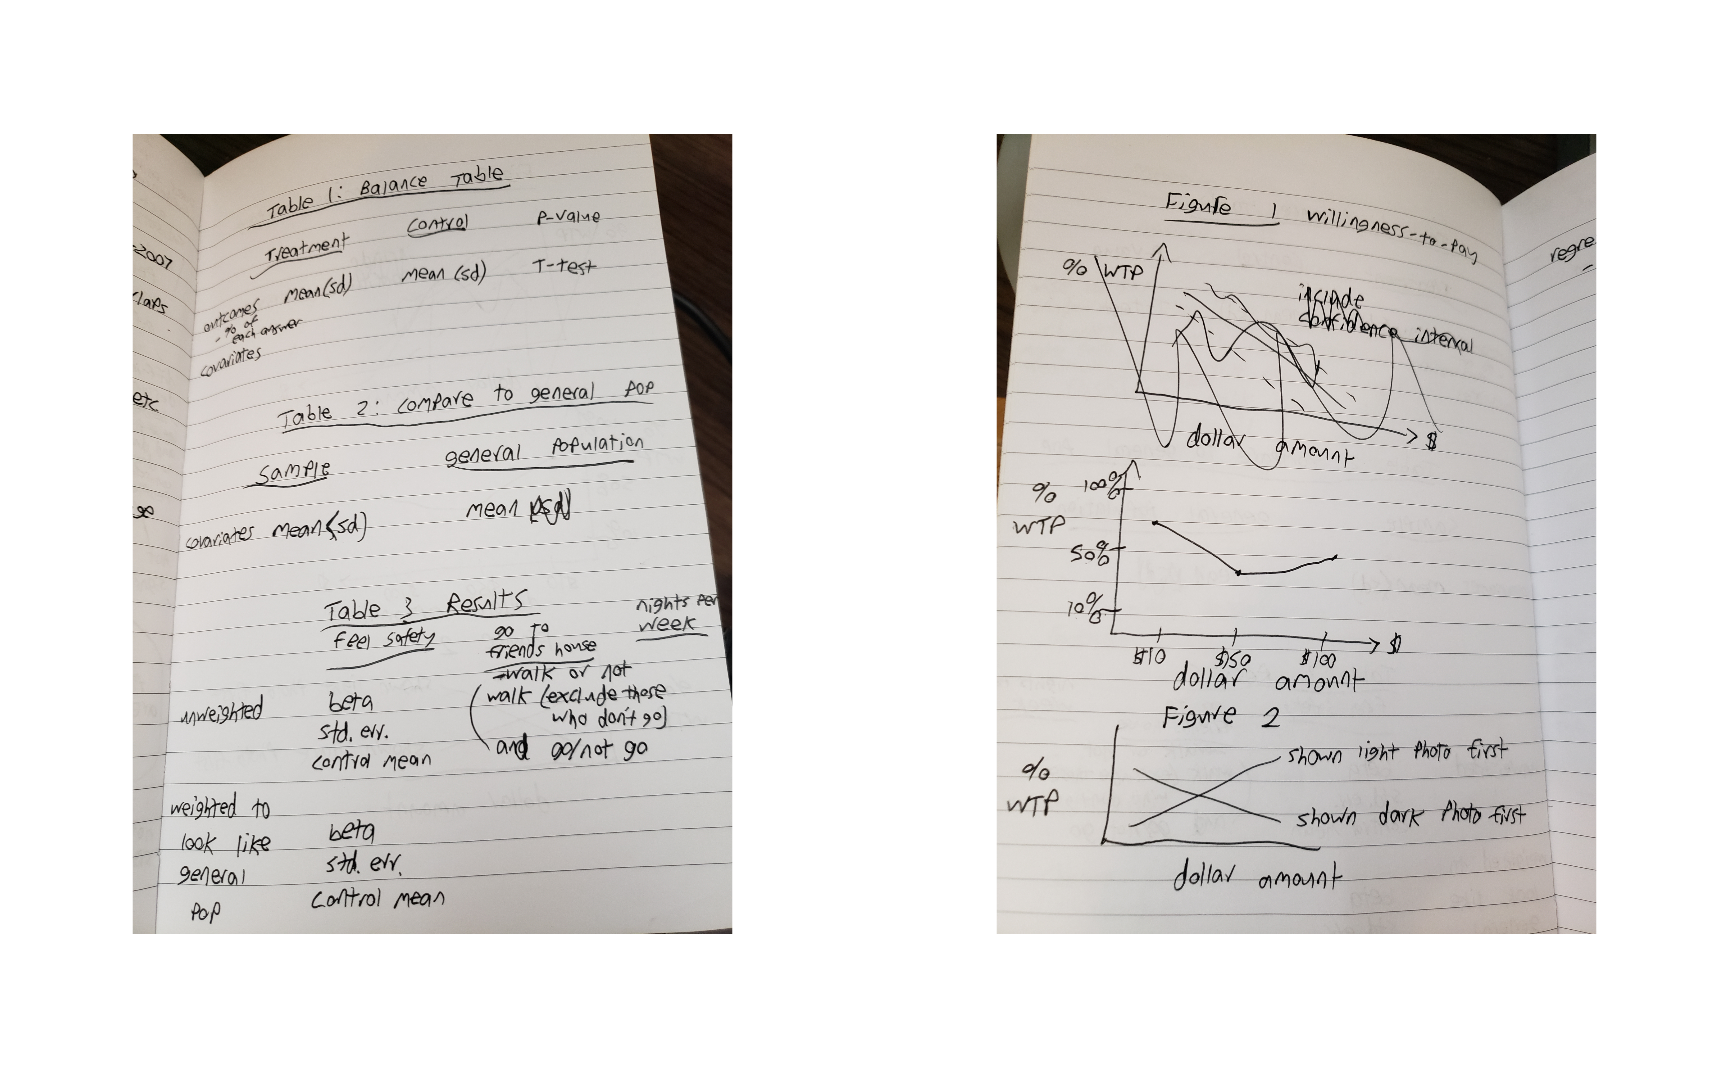
\includegraphics[width=1\linewidth,height=1\textheight,]{crimebythenumbers_files/figure-latex/unnamed-chunk-96-1} \end{center}

\hypertarget{r-projects}{%
\section{R Projects}\label{r-projects}}

We've talked about projects in an abstract sense - that they
are research papers or specific data exploration jobs.
RStudio provides, a bit confusingly, something called an R
Project, which is merely a helpful way to organize folders
for a specific project (paper, data exploration, etc.) that
you do. When you do a project, I recommend keeping
\emph{everything} for that project in a single folder on
your computer. Below is an image showing all of the folders
I use for my various R work. As you can see from the file
names, each folder is for a separate project, and there is
not overlap between them - each project is independent.

\begin{center}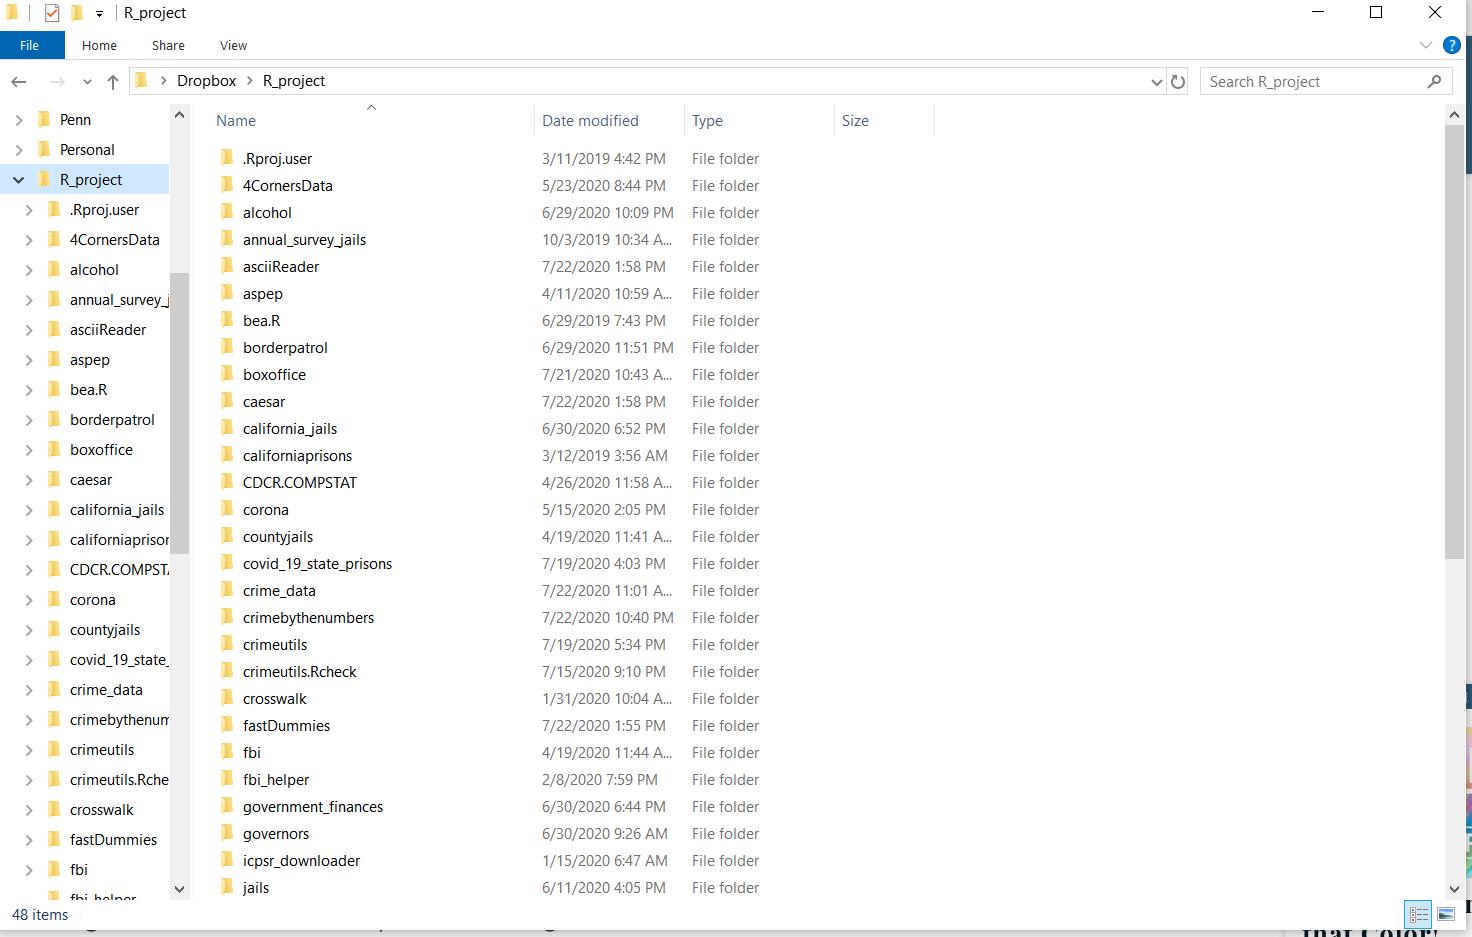
\includegraphics[width=1\linewidth,height=0.45\textheight,]{images/projects} \end{center}

First, I'll explain how to set up an R Project through
RStudio, and why you would want to do it. There are two main
reasons to want to use an R Project. First, throughout this
book I had you set your working directory so that R knew
where to look for a particular file. In R Projects, by
default the working directory is in that project's folder.
So if you had a file \texttt{example.csv} in your project
folder, you wouldn't need to set a working directory since R
would already be looking in that folder.

This may be a minor time-saving method if you're working
alone since you'd only need to set the working directory
once when not using an R Project. But consider if you're
collaborating with three people and you've shared your code.
When using an R Project, it just runs. Your collaborators
won't need to change the working directory to their own
directory. Second, it provides easy access to using the
version control software Git, which we'll talk about in
detail in Chapter @ref(git).

To make an R Project, start by clicking the \emph{File}
button on the top-left corner of RStudio and then click
\emph{New Project}. This will open up a window that has
three options: New Directory, Existing Directory, and
Version Control. New Directory says that the project we are
making is going to be in a brand-new folder that we're (R
will do this automatically) going to create. This is the one
you'll click on in the majority of cases. Existing Directory
is for making a folder in an existing folder, which doesn't
have too many useful cases. The Version Control is taking a
project that someone else has created and downloading it to
your computer. We'll cover this more in Chapter @ref(git).

\begin{center}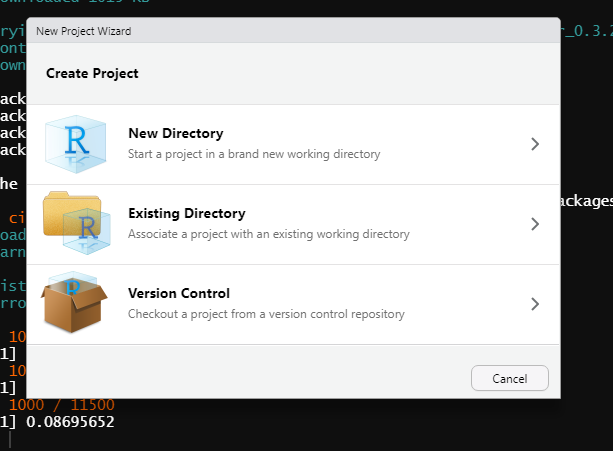
\includegraphics[width=1\linewidth,height=0.45\textheight,]{images/new_project_1} \end{center}

Once you've clicked New Directory, it'll change the window
to ask you what type of project you want. The following two
figures show all the different types of projects R can make
(installing some R packages, such as \texttt{bookdown}, can
add more types of projects to this list). R is very
versatile and has project types ranging from the standard R
Project to books and websites. We just want a standard
project so click the New Project button at the top.

\begin{center}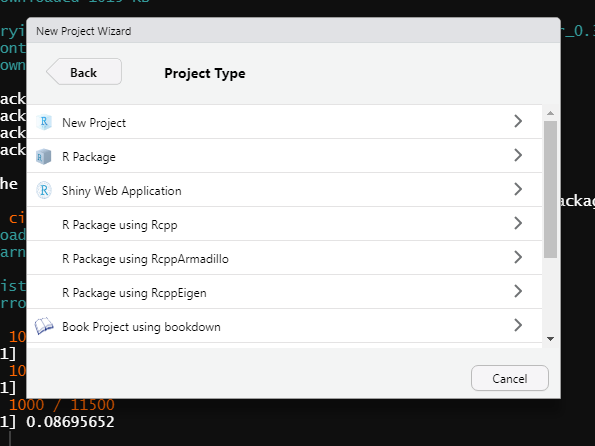
\includegraphics[width=1\linewidth,height=0.35\textheight,]{images/new_project_2} \end{center}

Now it'll have a window that says Create New Project up top.
In the Directory name: section you write the name of your R
Project. This will be the name of your folder so you want it
descriptive enough to understand (and for collaborators to
understand) what it is for, without being overly long. Once
you have a name you can click the Browse\ldots{} button on
the right and go to the folder on your computer where you
want to put this folder (ideally, you'll put it in a folder
that is backed up by something like DropBox). Make sure the
\emph{Create a git repository} checkbox is selected, and
we'll explain why in Chapter @ref(git). Click Create Project
and R will make the project folder on your computer and open
that project in RStudio.

\begin{center}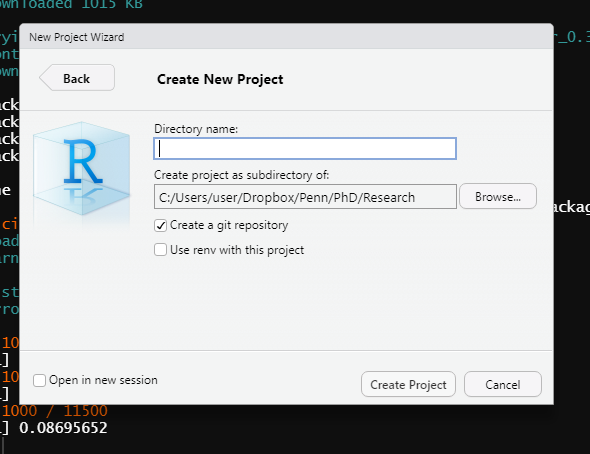
\includegraphics[width=1\linewidth,height=0.35\textheight,]{images/new_project_4} \end{center}

Below are images of a brand new R Project that I made called
\emph{example} that I put in my Desktop folder. The folder
is now empty except for two files - .gitignore (which we
won't talk about here) and \emph{example} which is type ``R
Project'' (and the full name would be \emph{example.Rproj}).
This is a \textbf{very} important file. Note that its name
is the same as the R Project name that I made, and the same
as the folder name on my computer. This file is essentially
a shortcut that you click to open that R Project. It doesn't
do anything more than open the R Project, but this is the
way you'll access the project every time you want to use it.
Double-click this and the R Project will open.

\begin{center}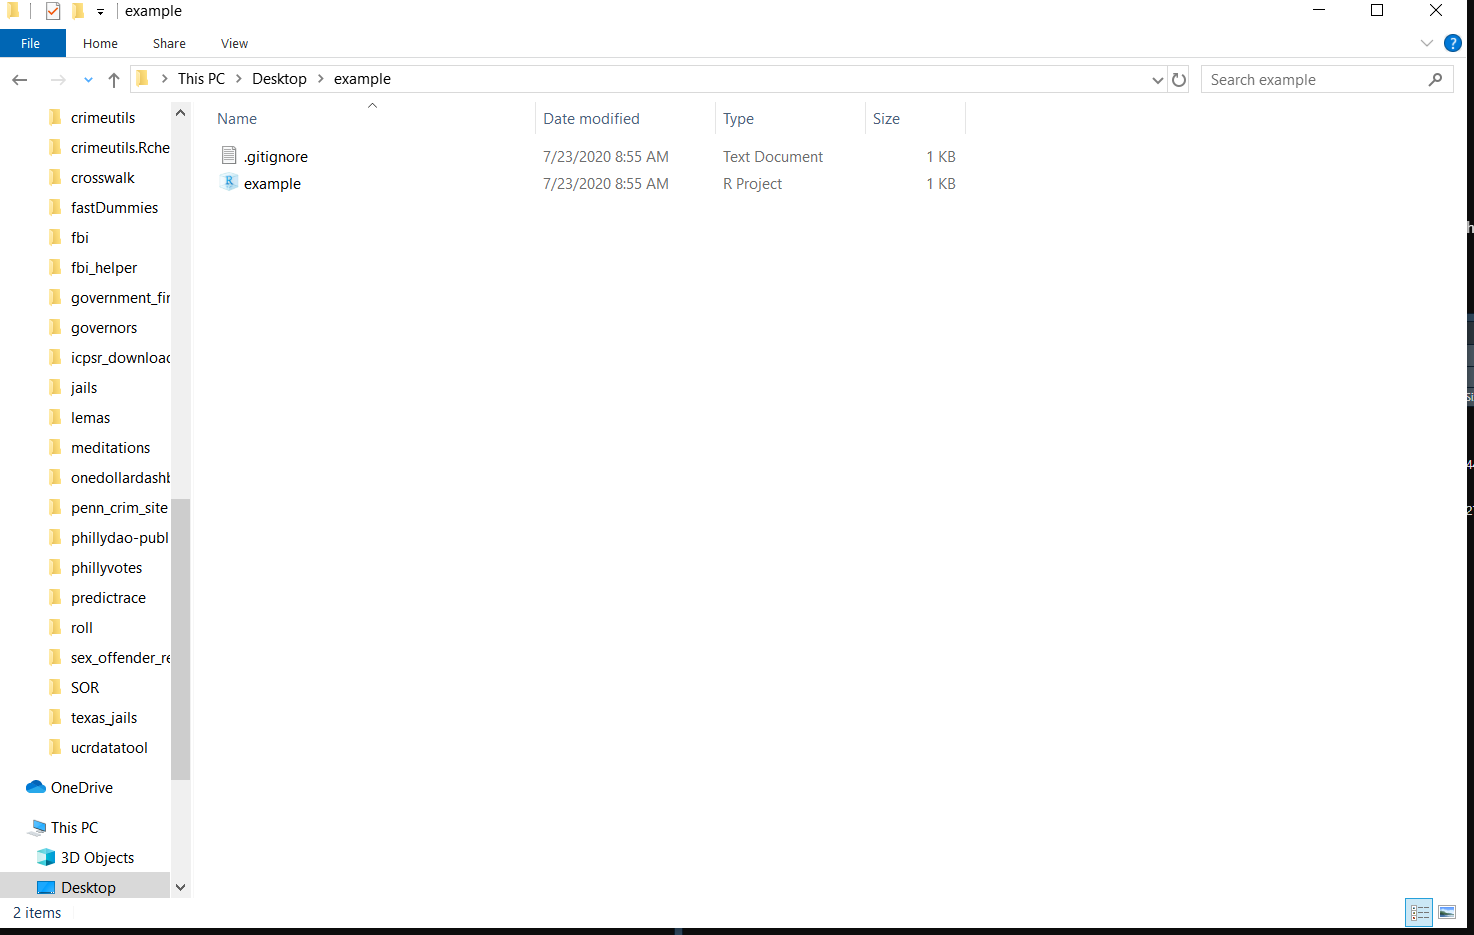
\includegraphics[width=1\linewidth,height=0.35\textheight,]{images/new_project_6} \end{center}

This RStudio session looks nearly identical to other
sessions that we've used - and it is nearly identical. A few
key differences can be found in the top-left corner where it
says ``example - RStudio,'' indicating that we're in the
\emph{example} R Project. And then directly below the
``Console'' tab it says ``C:/Users/user/Desktop/example/''.
This is the working directory of this project. I didn't set
it; R just knew where it was. If you move this folder to a
new folder (say, the Downloads folder) or if someone else
downloads it to their computer, R will automatically change
the working directory to the right one. You no longer have
to worry about it.

\begin{center}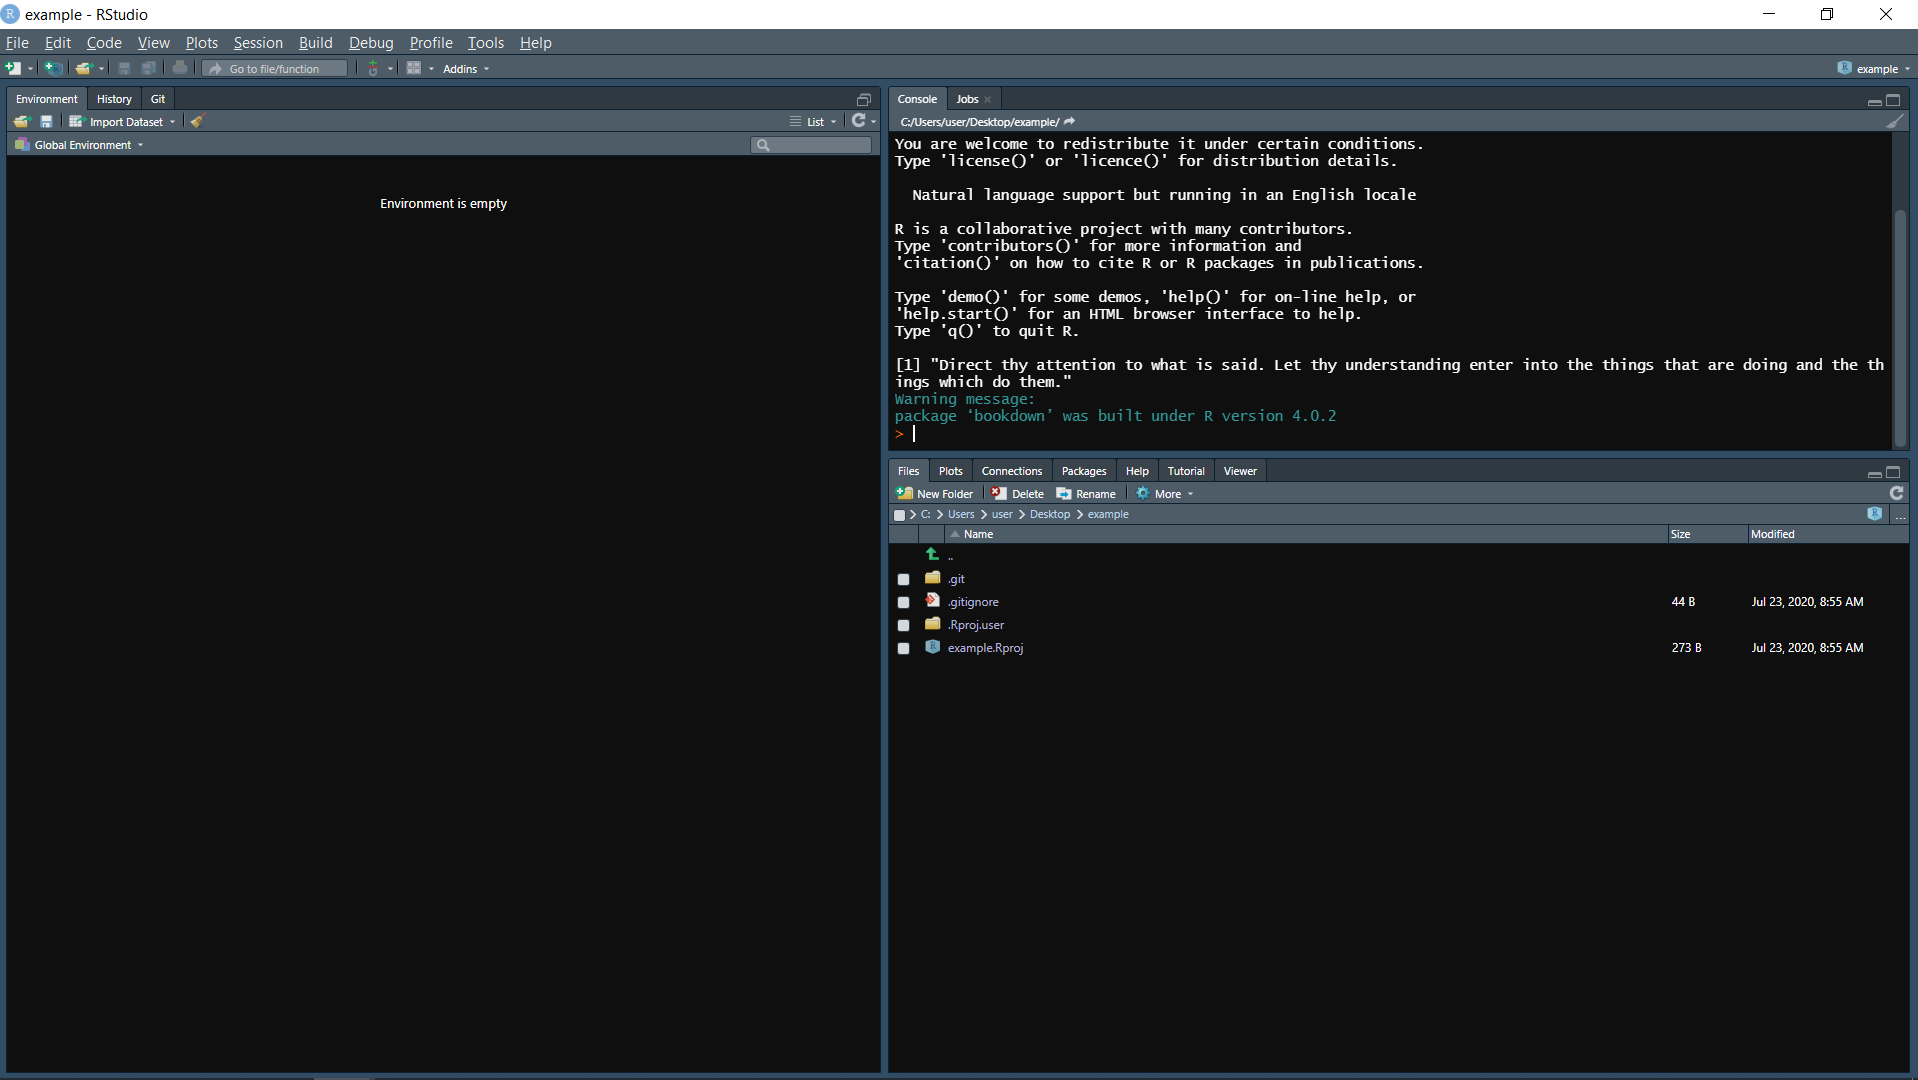
\includegraphics[width=1\linewidth,height=0.35\textheight,]{images/new_project_5} \end{center}

\hypertarget{folders}{%
\subsection{Folders}\label{folders}}

Now that we have the R Project made, we need to start adding
some R code and data files to the project so we can get
started working. But first, let's talk about proper ways to
organize the folder. I've added a few new folders to the new
\emph{example} R Project as the basic layout of my work
process. This is for a research-oriented project so it may
not apply in your particular case. Organizing your folders
(and as we'll see below, your code) is important so please
play around with different ways to organize and find a way
that works well for you.

\begin{center}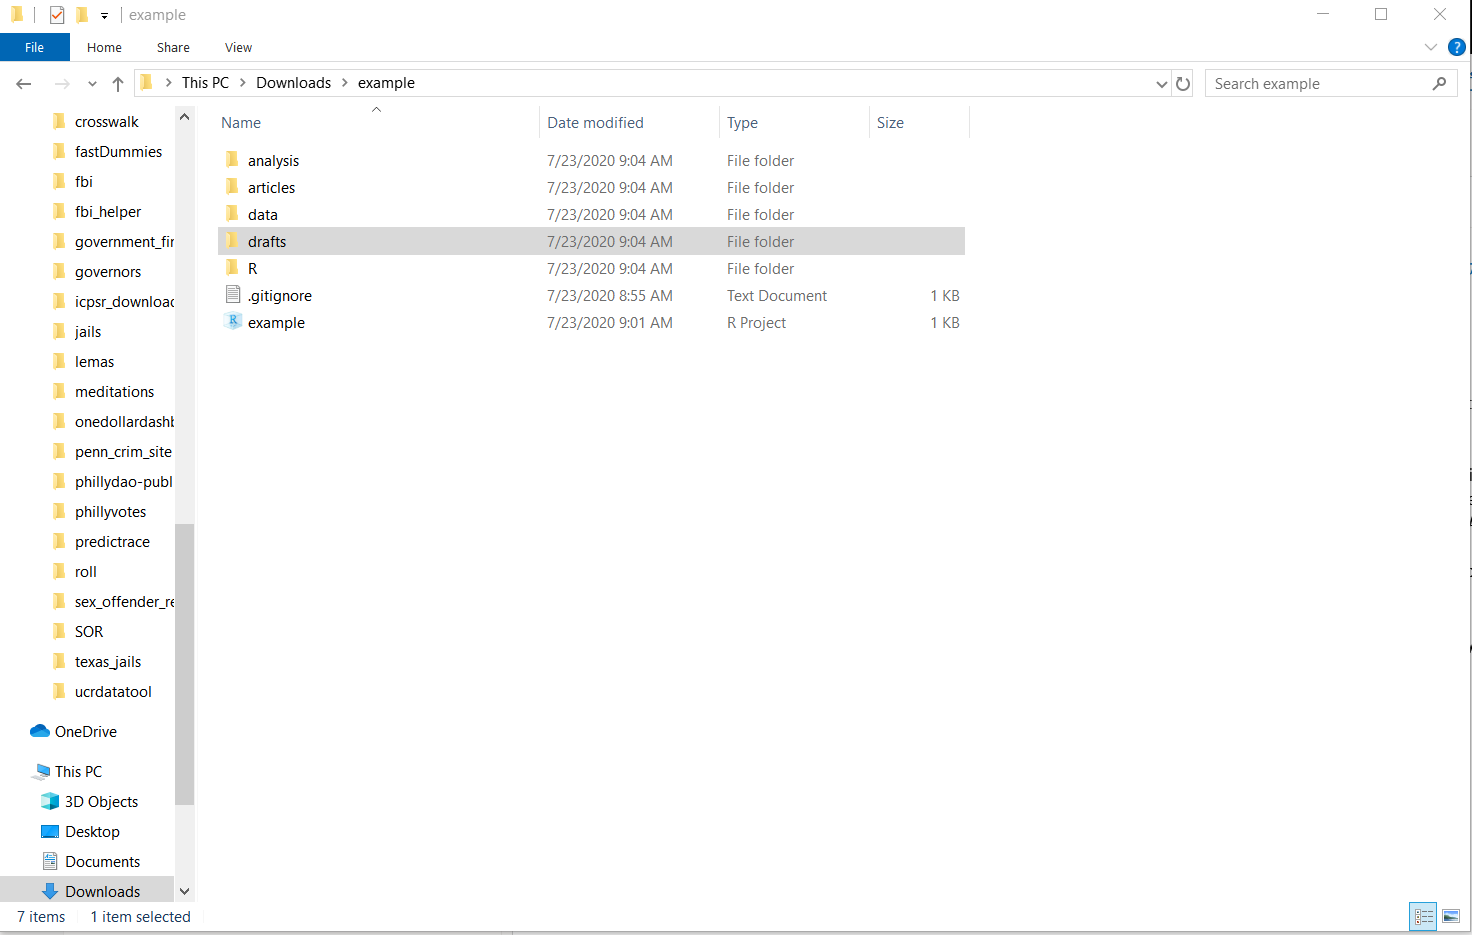
\includegraphics[width=1\linewidth,height=0.45\textheight,]{images/new_project_7} \end{center}

I've added five folders to the R Project folder: analysis,
articles, data, drafts, and R (note that I moved it to the
Downloads folder, and if I opened the project RStudio would
know where the new working directory was). I tend to do my
analysis using Stata (primarily because most of my
co-authors use Stata instead of R so this is a way we can
both work on the analysis) so in the analysis folder I'd
keep all of the .do (Stata) files to run the regressions. In
articles, I put PDFs of every article I read that I use (or
planned to use while reading it) for the paper I'm working
on in this project. It's good to keep this organized to
share with co-authors or just for easy reference after
you've read it. It certainly takes time to find good sources
for a lot of research, so you don't want to have to search
again because you've forgotten which article you had a
particular reference from or that was important to your
study. While I recommend writing your papers in R Markdown
(see Chapter @ref(r-markdown)), you will need to create
drafts of the paper to send to others (e.g.~your
collaborators or journals). The ``drafts'' folder is a good
place to keep these versions - some journals require that
you submit a Word Document with track-changes for a revise
and resubmit so you will need to leave R Markdown
occasionally to comply with these rules.

The final two important folders are ``R'' and ``data.'' In
the R folder - as you may have guessed - belong the various
R scripts that you write during the project. In Section
@ref(modular-r-scripts), we'll talk in detail as to how to
organize these scripts. Inside the ``data'' folder I made
two subfolders: ``raw'' and ``clean.'' The raw folder is
where you'll store the data exactly as you got it (for cases
where the data is acquired through webscraping, this isn't
necessary). This folder will have, for example, the PDFs
that you intend to scrape, or .csv files with crime data in
them. It is important to keep this data always unchanged
(change it only in R and save the output to a new file) so
you can replicate your results from the original data. In
the clean folder is that final data output from your work to
clean and manipulate (e.g.~subset, aggregate) the data. It
isn't strictly necessary to even output a final data set -
you could just rerun your code from the original data each
time, and this is fine if your code is very quick to run -
but it is important both for safekeeping and to be able to
share with others. If you collaborate with people, you'll
want to be able to send them the data so they can examine it
without having to run all of your code themselves.

\begin{center}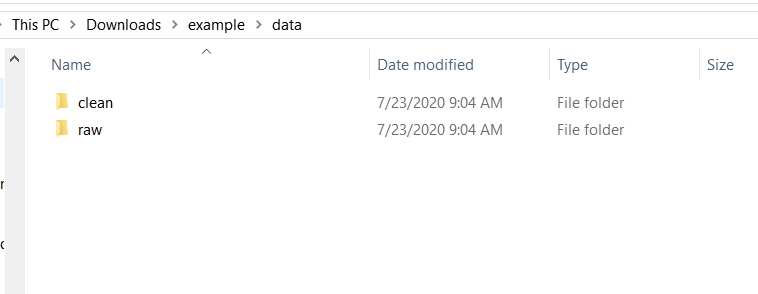
\includegraphics[width=1\linewidth,height=0.45\textheight,]{images/new_project_8} \end{center}

\hypertarget{modular-r-scripts}{%
\section{Modular R scripts}\label{modular-r-scripts}}

If you are like many people who start programming, all of
your code will be in a single R script. This is fine when
you're first getting familiar with R and don't want to go
searching for code in places when you're still uncomfortable
with the language. As you become more familiar with R - and
as your projects get more complex - you'll want to start
making multiple R scripts in a single project.

When you're writing a paper you don't just write one
extremely long sentence. You break up ideas into paragraphs
and divide groups of paragraphs into larger sections. This
is useful in a paper to organize your thoughts and to make
it readable for others. It's also useful when working since
you know, for example, ``Section 1 is done, but I still need
to finish Section 2 and the last part of Section 3.'' This
way you don't confront working on the entire paper at once.
You'll want to follow these lessons in the code you write,
with each ``section'' of code being its own R script and
within a script split up code into particular
``paragraphs.'' The end goal should be to have modular R
scripts, with each script being independent (or relatively
so) and the combination of these parts has all the code for
your particular project. This is a bit of an abstract
concept so let's use a real example from one of my recent
projects.

\begin{center}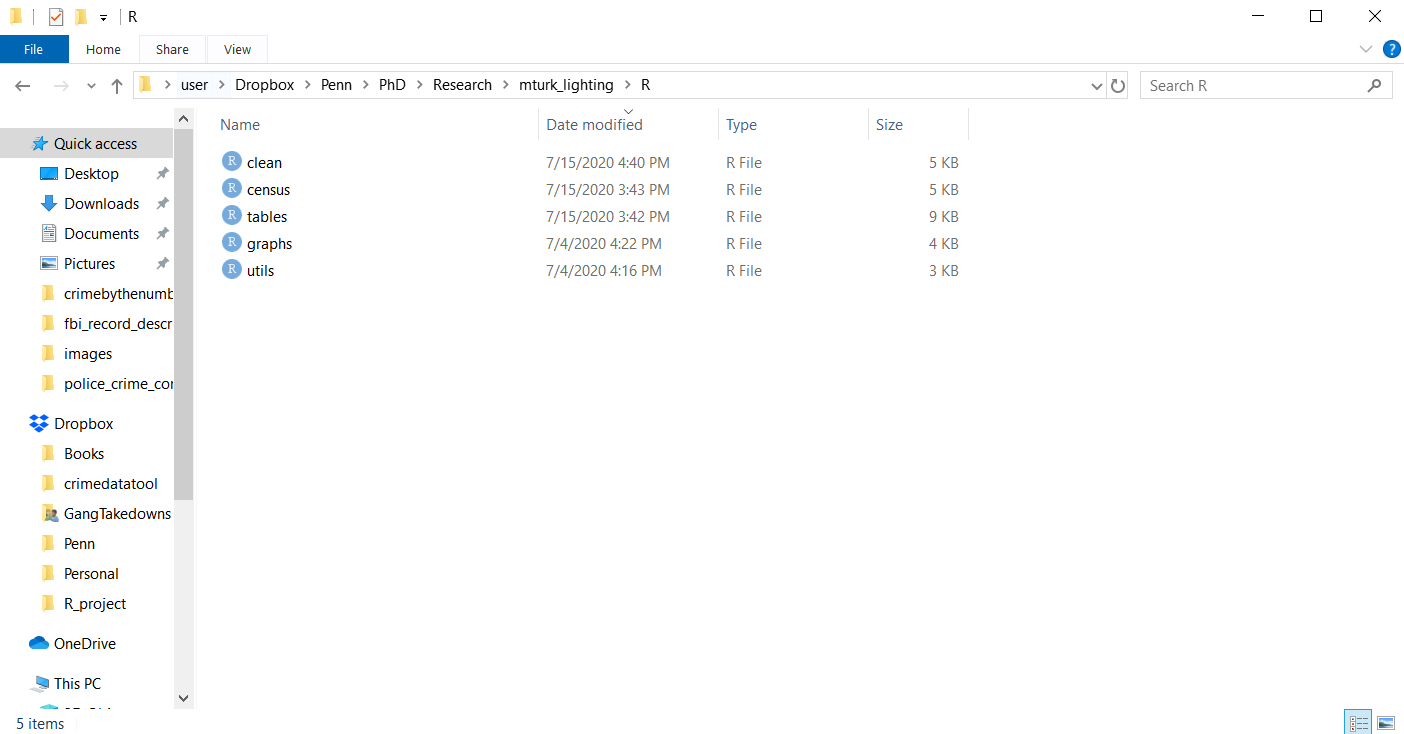
\includegraphics[width=1\linewidth,height=0.45\textheight,]{images/modular_scripts} \end{center}

Above is a folder for the code used to analyze data for a
paper examining perceptions of outdoor lighting. There are
five R scripts in the folder - clean.R, census.R, tables.R,
graphs.R, and utils.R - and these are the only ones used for
this project.\footnote{The analysis was done in Stata so
  there are separate files for that.} Each of these files
(utils.R is an exception) has a particular role to play in
the analysis of the data. The first file, clean.R is just
code that cleans up the survey data and makes it ready to be
analyzed and graphed. The census.R file has code that cleans
Census data that my co-author and I use to compare our
survey sample to the general public. As this is a separate
data set than the survey data, I have it in its own R
script. tables.R and graphs.R are the code to make
descriptive statistics tables and figures for the paper,
respectively. I chose these files because they are doing
fairly separate tasks, all with the goal of turning raw data
into a research paper.

This is an example of how I approach making R scripts, not
necessarily the best way to do so. Even here, other
decisions could be made. For example, I could have put the
code from census.R into clean.R since they're both about
cleaning data. While you should try to make separate R
scripts for broadly different tasks (regardless of how much
code that task requires), you should experiment with how you
prefer to separate these scripts, and balance between having
one (or a few) super scripts that comprise everything with
having too many scripts that do too little - this balance
requires experience and experimentation so keep at it!

\hypertarget{modular-code}{%
\section{Modular code}\label{modular-code}}

In addition to having separate scripts for each major part
of your project, you will want to organize each individual
script into relatively modular parts. Whereas each script is
like a book chapter, the code inside the script should be
like paragraphs, separated into distinct chunks. For
example, let's say you have some raw data and want to subset
it, change some values (e.g.~renaming F to Female, M to
Male), and then aggregate to a larger geographic area. This
is a three-step process - subset, change, aggregate - so
you'll want to have three different parts of your R script
dedicated to this. Now, if this is a simple process (and it
will always depend on the data and what you want to do with
it), you may want to have each step in its own Section (as
we'll discuss next). If it's relatively simple and takes
only a few lines per step, you'll likely just want to have a
line break between steps and identify your choices in
comments. It's hard to give precise rules on how to do this
as it really does depend on personal preference - I think
having more comments and line breaks early in your R career
is best as you're still learning R, and it is good practice
to comment your code. You can always alter this balance to
suit your preferences as you gain more experience.

The goal of making modular code is to avoid having a large
amount of code without breaks or comments - that'd be like
reading a run-on sentence. We'll talk about comments more in
Section @ref(comments), but here you should explain your
choices (e.g.~``Subset to only violent crime and property
crime'') to inform collaborators (other people and yourself
in the future who will likely forget what or why you did
something), but without writing too much. Generally the rule
of thumb is to have comments for why you did something, not
explaining what you did. I think a mix of what and why is
helpful as it's quicker than looking at the code, especially
if your code is complex. Like a lot of your work, however,
this depends on the project and your audience - if you're
working with someone new to R, having more comments
explaining what you did is helpful.

\hypertarget{section-labels}{%
\subsection{Section labels}\label{section-labels}}

When you have major parts of an R script, you should have
something to indicate that this is a distinct section from
other parts. RStudio has a handy tool to help make that
distinction by creating sections in your R script. Press the
keys Control+Shift+R (Command+Shift+R in a Mac), and it will
open up a window where you can set a section label. Write
the name of the section you want and click OK, and it'll add
that to where your cursor was in the R Script. You can also
do this by simply adding four dashes on the end of a
comment.

\begin{center}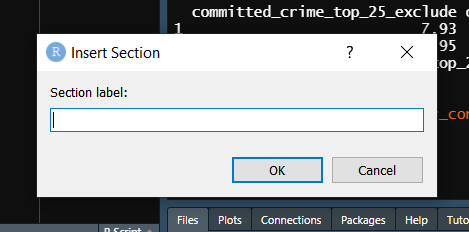
\includegraphics[width=1\linewidth,height=0.45\textheight,]{images/section_label1} \end{center}

Sections are more than just commented parts of a Script.
Note that in the following screenshot, there is both the
Section label in the R Script and that same label in a new
section of the Source tab on the right. You can get to this
section by clicking on the button on the very top right, the
one that looks like a bunch of misaligned lines. In here, it
shows all the Sections that exist and clicking the Section
name will move to the start of that Section in your R
Script. If you have a long script (which is generally
unadvised but sometimes can't be helped), this is an easy
way to find a particular part of your code.

\begin{center}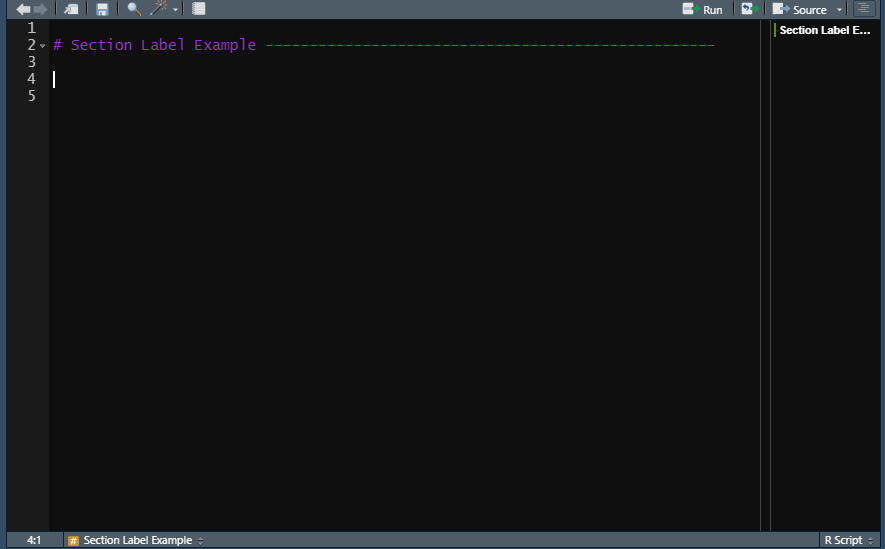
\includegraphics[width=1\linewidth,height=0.45\textheight,]{images/section_label2} \end{center}

\hypertarget{helper-r-scripts}{%
\subsection{Helper R scripts}\label{helper-r-scripts}}

As part of making code organized, I find it helpful to make
an R script in each (or most) of my projects to hold helper
functions or objects - and I call this utils.R (utils stands
for utility as these are helpful pieces of code for the
project). This file should be for code that will be used in
multiple R Scripts, so you want them in a single place
rather than copying them over in each script where you need
them.

In utils.R, I keep functions that are either auxiliary (such
as code to check data by printing out a set of outputs) or
code that is used infrequently (such as loading several
files and merging them together at the start of an R script)
where I don't want them in the main file. I also include
useful objects such as a vector of values that I will use to
subset. For example, if I wanted to subset all violent
crimes from a data set, I would need to know what crimes in
that data are considered violent, put them as strings in a
vector, and subset to only rows that match those strings. I
could make an object with this vector, such as
\texttt{violent\_crimes\ \textless{}-\ c("murder",\ "rape",\ "robbery",\ "assault")}.

If you want to run utils.R (or any .R file) in a different R
script, you can use the \texttt{source()} function, which
makes R run the entire script inputted in the parentheses.
Just put the file name (in quotes) in the parentheses and it
will run. For example, if we want to run utils.R, we'd write
\texttt{source("utils.R")}. If that file was in the ``data''
folder of our R Project, we'd write
\texttt{source("data/utils.R")} so R knew to look in the
``data'' folder for the file.

It isn't necessary to make helper functions like these, but
I find them helpful. I recommend that you try them out when
you do R projects, but if you don't find them useful please
feel free to stop using them.

\hypertarget{collaboration}{%
\chapter{Collaboration}\label{collaboration}}

\hypertarget{code-review}{%
\section{Code review}\label{code-review}}

When you collaborate with other people, you will probably
each be working on a separate (though related) part of the
project and then will combine each part when you are done.
Combining your code could be through emailing each other R
scripts - and having one person combine everything - or
something more formalized such as using Git, which we
discuss in Chapter @ref(git). However you decide to do this,
it is important to use a process to review your
collaborator's code (and have them review yours) to check
for mistakes.\footnote{If your collaborator does not know R,
  they should read this book.} This is a similar process to
having a colleague read a paper draft before submitting it.

Code review is a useful technique for reducing the number of
mistakes as it is a check on the work before using the code
for real. Code review generally involves having one person
who writes the code send it to another person who checks the
code for any potential mistakes or issues. This check
involves ensuring that the code meets the specified style
(this is discussed further in Section
@ref(style-guidelines)) and that there are no bugs (which
are errors in the code). For the person having their code
reviewed, having comments explaining the what and why of the
code (discussed more in Section @ref(comments)) will help
the reviewer quickly go through the code. The code should
also be relatively short, comprised of a specific R script
(or related scripts) and no more than a few hundred lines of
code. This is because as code gets more interrelated and
complex, it is harder for someone unfamiliar with the code
to understand it and see any issues. That means that a
reviewer for long code is more likely to miss issues and
take longer to review. Reviewing shorter code, even if that
means reviewing more often, is often far more efficient for
both the reviewer and reviewee and catches more issues.

In cases where you have unit tests (which are discussed in
Chapter @ref(tests)) written for the code, these tests are
an automated form of code review as they too check for
mistakes. To save people's time, you should avoid sending
the code for review until it passes all unit tests. However,
if you're stuck and can't get certain tests to pass, working
with someone else to solve the problem is often faster than
doing so yourself because then you have an outside
perspective who may see something that you missed.

For code review to be most efficient, I recommend developing
some rules with your collaborators to specify how and when
code review is done. For example, you should determine who
reviews certain people's code (ideally with senior people
reviewing junior people's code) and how often it is done. I
believe that doing code reviews relatively frequently
(i.e.~after a working draft of some code is ready) is useful
as you can catch issues early and not waste anyone's
(especially the person writing the code) time. However,
having hard time limits is probably ill-advised as sometimes
writing certain code takes far longer than expected and
reviewing an unfinished (and potentially far from finished)
bunch of code is not efficient for anyone.

When someone is reading a draft of your research paper, they
are generally looking for whether it is correct (i.e.~your
methods are right, the lit review is thorough, etc.) and how
well it flows. Code review is the same. While the primary
goal is finding errors, an important aspect is to ensure
that it is readable (i.e.~proper spacing, how names are
written) and consistent across everyone's code in that
group. More formally, ensuring that everyone's code is
readable and consistent is having people follow a style
guideline.

\hypertarget{style-guidelines}{%
\subsection{Style guidelines}\label{style-guidelines}}

An important part of reviewing people's code is ensuring
that everyone is following the same style guidelines when it
comes to writing code. Style guidelines are the grammar
rules of writing code. They dictate (or encourage) certain
style choices, such as whether object names are lowercase,
whether they include punctuation, and even when to put long
code on a new line. This is equivalent to making sure that
people writing in plain language put punctuation and
capitalization in the expected place. While you can read
!SomEThiNg WrITen. LiKE thIs, it is easier to understand
when it follows adopted and accepted rules.

The important thing here is to be consistent. Consistency
makes code much easier to read and helps make code written
by multiple people more interchangeable. This book follows
the \href{https://style.tidyverse.org/}{tidyverse style
guide,} which is one that many R programmers follow, but the
exact style you choose is relatively unimportant (choosing
more common styles helps when your code may be used by
people out of your organization). Feel free to adopt an
already-made style guide, make any modifications to suit
your preferences, or to create an entirely new one yourself.
As long as people follow the same format, you'll be able to
spend more time on the code, and less time trying to
understand it.

\hypertarget{documentation}{%
\section{Documentation}\label{documentation}}

An important, though occasionally tedious, part of writing
code is documenting your work. We'll talk about
documentation in two ways, through comments, which focus on
specific parts of code, and vignettes, which document the
project more broadly.

\hypertarget{comments}{%
\subsection{Comments}\label{comments}}

In Section @ref(using-rstudio) we introduced comments, which
are essentially notes about the code that you include in an
R script (by starting a line with the pound key \#) that
isn't run. They are just ``comments'' to yourself or anyone
else reading the code to explain what that code does and why
it is there. As is often repeated in explaining the benefit
of comments, the main collaborator you will have is yourself
in the future.\footnote{I recently worked on a follow-up
  paper to one I had done a year ago. For some reason, past
  me decided to name some functions based on the authors of
  a paper that created that particular method, and didn't
  leave comments explaining what the code did or why. Past
  me caused a lot of problems for current me. Please comment
  your code!} You don't need to comment on every single line
of code - and doing so would just make it hard to read - but
you should comment on important things or chunks of code
(i.e.~several lines of code that all are for the same
purpose). If you write a function, you'll want at least a
brief comment explaining what it does and what the inputs
and parameters do.

Writing comments is not as fun as writing code. Stopping to
write a comment on something that seems obvious at the time
(after-all, you figured out how to do something you wanted
to do and likely were focusing on) interrupts the flow of
writing code and slows down your work. And when you have
looming deadlines and multiple projects that you're working
on, spending the time writing good comments may seem like a
bad use of time as the payoff is only in the future.
However, the benefits far outweigh the cost. This is true
for two reasons. First, when you're collaborating with
others, it is much quicker to have text explaining the code
than to walk through the code with them (or to have them try
to figure it out themselves).\footnote{This is one of the
  main reasons I wrote this book. After a few years of
  helping Penn students with the same questions, I decided
  to write out guides to those topics.} As you work with
more people, comments become increasingly important. Writing
good comments is also time-efficient when considering that
in many cases when you do research you will have to return
to the project in the future.

This is best shown when considering a research project that
leads to a journal article. For many papers, even if you are
fantastically productive and can work nonstop at it without
forgetting any decisions, at a certain point you'll need to
finish and submit it to a journal. Journal reviews can often
take three to six months so at that point you'll likely have
forgotten many of the (seemingly obvious) decisions you made
in the course of the project.\footnote{If you're like me and
  on your seventh rejection for a particular paper, three to
  six months may be optimistic.} Having comments explaining
why you made a certain decision (such as including or
excluding certain crime types from your analysis) can be a
huge time-saver when addressing reviewer concerns - you will
know why each decision was made and won't have to try to
figure out the \emph{why}. This is particularly important
when you have to defend a decision in which there is no
obvious choice and you want to know your thought process at
the time you wrote the code and were immersed in the issues
of the data. A lot of data decisions are reasonable at the
time based on the quirks of the data but can appear to make
no sense if you aren't familiar with the data - comments can
remind you of the quirkiness and how you handled it.

\hypertarget{vignettes}{%
\subsection{Vignettes}\label{vignettes}}

Vignettes are essentially a document that explains how to do
something with the code you have written. This is common
when someone has written an R package and they want to
explain in detail important functions from the package. You
can think of chapters of this book as vignettes covering
particular topics - PDF scraping, webscraping, regular
expressions, etc. To make a vignette, you can make an R
Markdown file (for more information on R Markdown please see
Chapter @ref(r-markdown)) detailing that topic. Since the
text you write is included in the document, these files are
basically normal R scripts with extensive comments written
in plain language. Often, these comments are more formal
than what you'd write in an R script as they are written as
complete sentences or paragraphs and walk through
comprehensive ideas rather than focus on discrete chunks of
code.

One increasingly prominent method of using R for research is
to do everything in an R Markdown file. This allows you to
explain your approach - including context on why you did
something - and each step you took in plain language in the
text of the R Markdown file while still including the code
directly in the file. Whether you include the code in the
output (e.g.~a PDF or Word Document), or just the result of
the code (e.g.~a graph or table), depends on your audience
and how far along you are in the project.

If this is for a presentation to update collaborators, for
example, it is useful to include the code as they may notice
an issue or give advice based on the code. Including code
can also teach your audience something new (I've certainly
learned a lot by watching people present using code I wasn't
familiar with). If the document is for an audience
unfamiliar with R (or programming more generally), or where
time to present is limited, you probably won't want to
include code.

Whether you do your work in an R script or in an R Markdown
file is up to you. If you intend to write up a report
anyway, having everything written up in the R Markdown file
as you write your code can save you time as you're merging
the code and the writing process. However, this loses some
nice features in R such as unit tests, which we will discuss
in detail in Chapter @ref(tests). It also depends on how
complex your project is. If you have code that is hundreds
of lines long and spans multiple R scripts, putting it all
into a single R Markdown file is unfeasible. In this case
it'd be better to run the code in the R scripts and use the
R Markdown file just to present results.

\hypertarget{r-markdown}{%
\chapter{R Markdown}\label{r-markdown}}

When conducting research your end product is usually a Word
Document or a PDF which reports on the research you've done,
often including several graphs or tables. In many cases
people do the data work in R, producing the graphs or
numbers for the table, and then write up the results in Word
or LaTeX. While this is a good system, there are significant
drawbacks, mainly that if you change the graph or table you
need to change it in R \textbf{and} change it in the report.
If you only do this rarely it isn't much of a problem.
However, doing so many times can increase both the amount of
work and the likelihood of an error occurring from
forgetting to change something or changing it incorrectly.
We can avoid this issue by using R Markdown, R's way of
writing a document and incorporating R code within.

This chapter will only briefly introduce R Markdown, for a
comprehensive guide please see
\href{https://bookdown.org/yihui/RMarkdown/}{this excellent
book.} For a cheat sheet on R Markdown see
\href{https://www.rstudio.com/wp-content/uploads/2015/02/RMarkdown-cheatsheet.pdf}{here.}

What R Markdown does is let you type exactly as you would in
Microsoft Word and insert the code to make the table or
graph in the places you want it. If you change the code, the
document will have the up-to-date result already, reducing
your workload. There is some additional formatting you have
to do when using R Markdown but it is minimal and is
well-worth the return on the effort. This book, for example,
was made entirely using R Markdown.

I include this chapter early in the book - and likely before
you are really comfortable with using R - since some new R
programmers do like to do all of their work using this
method. In my experience this is relatively rare, but I
still wanted to make the info available for those that do.
For new programmers I recommend reading this chapter so you
understand R Markdown, but still use normal R scripts when
writing code - don't use R Markdown for everything. Focus on
learning how to write good code before adding the complexity
of writing full documents using R Markdown.

To open up an R Markdown file click File from the top menu,
then New File, and then R Markdown\ldots{}

\begin{center}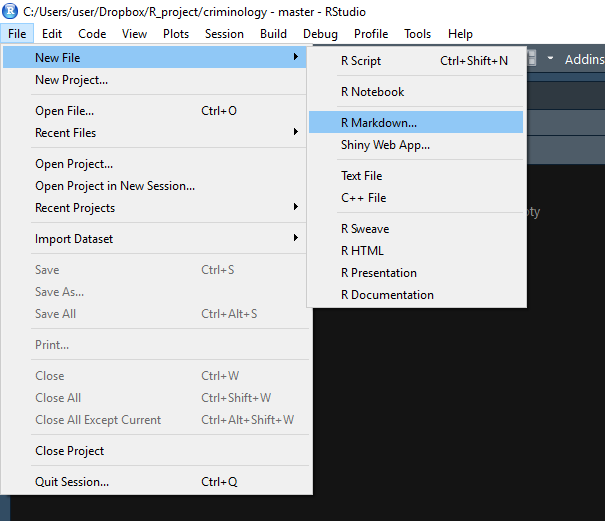
\includegraphics[width=1\linewidth,height=0.4\textheight,]{images/markdown1} \end{center}

From here it'll open up a window where you select the title,
author, and type of output. You can always change all three
of these selections right in the R Markdown file after
making your selection here. Selecting PDF may require you to
download additional software to get it to output - some
operating systems may already have the software installed.
For a nice guide to making PDFs with R Markdown, see
\href{https://medium.com/@sorenlind/create-pdf-.reports-using-r-r-markdown-latex-and-knitr-on-windows-10-952b0c48bfa9}{here.}

\begin{center}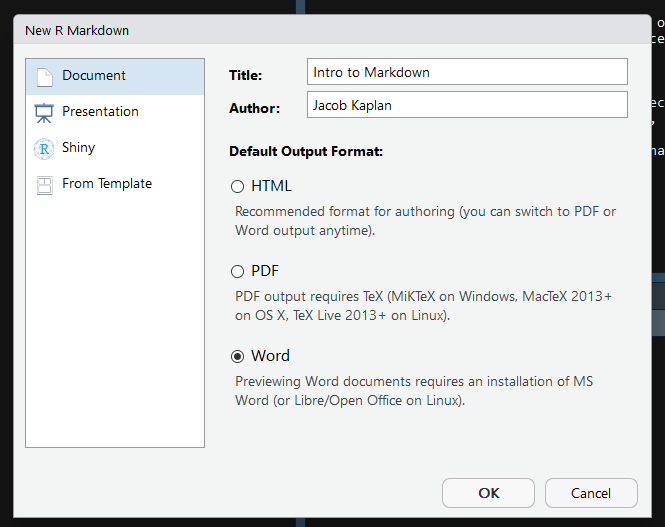
\includegraphics[width=1\linewidth,height=0.4\textheight,]{images/markdown2} \end{center}

When you click OK, it will open a new R Markdown file that
is already populated with example text and code. You can
delete this entirely or modify it as needed.

\begin{center}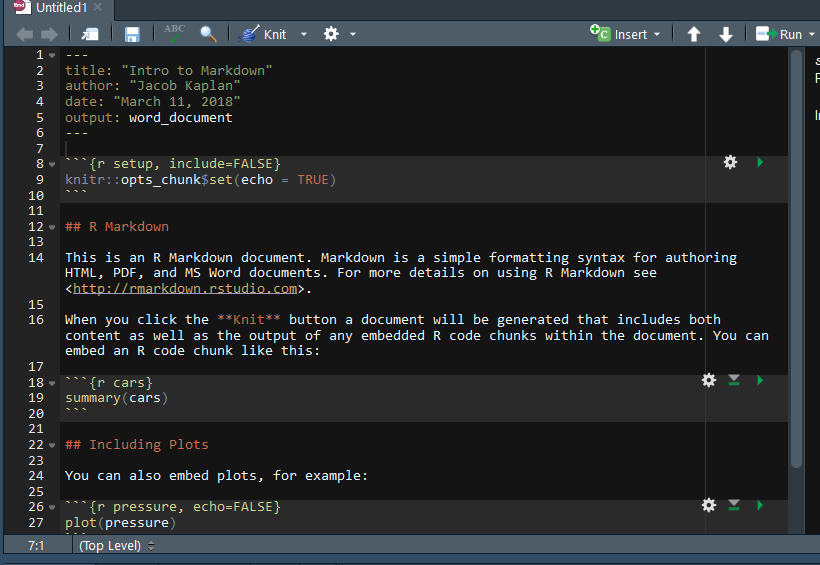
\includegraphics[width=1\linewidth,height=0.4\textheight,]{images/markdown6} \end{center}

When you output that file as a PDF it will look like the
image below.

\begin{center}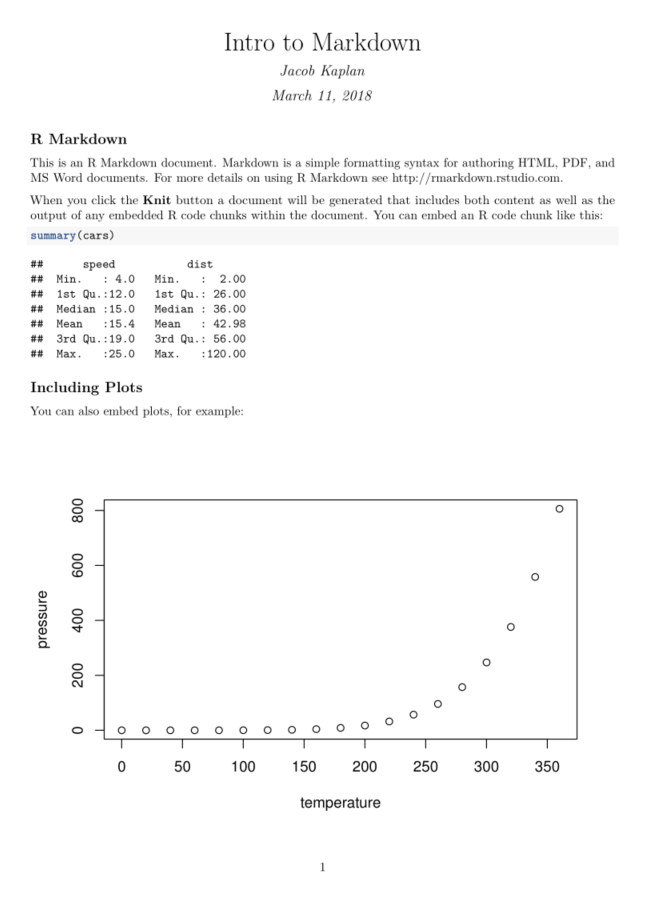
\includegraphics[width=1\linewidth,height=1\textheight,]{images/markdown_output_example} \end{center}

R converted the file into a PDF, running the code and using
the formatting specified. In an R Script a \texttt{\#} means
that the line is a comment. In an R Markdown file, the
\texttt{\#} signifies that the line is a section header.
There are 6 possible headers, made by combining the
\texttt{\#} together - a \texttt{\#} is the largest header
while \texttt{\#\#\#\#\#\#} is the smallest header. As with
comments, they must be at the beginning of a line.

The word ``Knit'' was surrounded by two asterisks \texttt{*}
in the R Markdown file and became bold in the PDF because
that is how R Markdown sets bolding - to make something
italics using a single asterisks like \emph{this}. If you're
interested in more advanced formatting please see the book
or cheat sheet linked earlier.

Other than the section headers, most of what you do in R
Markdown is exactly the same as in Word. You can write text
as you would normally and it will look exactly as you write
it.

\hypertarget{code-1}{%
\section{Code}\label{code-1}}

The reason R Markdown is so useful is because you can
include code output in the file. In R Markdown we write code
in what is called a ``code chunk''. These are simply areas
in the document which R knows it should evaluate as R code.
You can see three of them in the example - at lines 8-9
setting a default for the code, lines 18-20 to run the
\texttt{summary()} function on the \emph{cars} data (a data
set built into R), and lines 26-28 (and cut off in the
screenshot) to make a plot of the data set \emph{pressure}
(another data set built into R).

To make a chunk click Insert near the top right, then R.

\begin{center}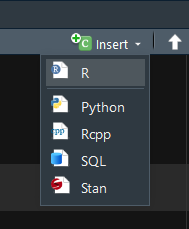
\includegraphics[width=1\linewidth,height=0.45\textheight,]{images/markdown3} \end{center}

It will then make an empty code chunk where your cursor is.

\begin{center}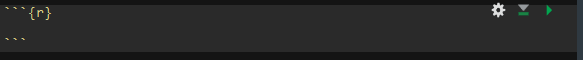
\includegraphics[width=1\linewidth,height=0.45\textheight,]{images/chunk_example} \end{center}

Notice the three ` at the top and bottom of the chunk. Don't
touch these! They tell R that anything in it is a code chunk
(i.e.~that R should run the code). Inside the squiggly
brackets \texttt{\{\}} are instructions about how the code
is outputted. Here you can specify, among other things if
the code will be outputted or just the output itself,
captions for tables or graphs, and formatting for the
output. Include all of these options after the \texttt{r} in
the squiggly brackets. Multiple options must be separated by
a comma (just like options in normal R functions).

If you do not have the R Markdown file in the same folder as
your data, you'll need to set the working directory in a
chunk before reading the data (you do so exactly like you
would in an R Script). However, once a working directory is
set, or the data is read in, it applies for all following
chunks. You will also need to run any packages (using
\texttt{library()}) to use them in a chunk. It is good form
to set your working directory, load any data, and load any
packages you need in the first chunk to make it easier to
keep track of what you're using.

\hypertarget{hiding-code-in-the-output}{%
\subsection{Hiding code in the
output}\label{hiding-code-in-the-output}}

When you're making a report for a general audience you
generally only want to show the output (e.g.~a graph or
table), not the code that you used. At early stages in
writing the report or when you're collaborating with someone
who wants to see your code, it is useful to include the code
in the R Markdown output.

If you look at the second code chunk in the screenshot
(lines 18-20) it includes the function
\texttt{summary(cars)} as the code and the options
\texttt{\{r\ cars\}} (the ``cars'' simply names the code
chunk ``cars'' for if you want to reference the chunk - or
its output if a table or graph - later, but does not change
the code chunk's behavior). In the output it shows both the
code it used and the output of the code. This is because by
default a code chunk shows both. To set it to only show the
output, we need to set the parameter \texttt{echo} to FALSE
inside of the \texttt{\{\}}.

In the third code chunk (lines 26-28), that parameter is set
to false as it is \texttt{\{r\ pressure,\ echo=FALSE\}}. In
the output it only shows the graph, not the code that was
used.

\hypertarget{inline-code}{%
\section{Inline Code}\label{inline-code}}

You can also include R code directly in the text of your
document and it will return the output of that code. To use
it, you need to setup an inline code chunk using the tick
mark followed by the lowercase letter R, the code you want
to use, and then end it using another tick mark. This is
called using inline code. When you have a table or
visualization to output, this isn't the proper method, it is
best for small pieces of text to add to your document. This
is most useful for when you want to include some descriptive
info, such as the number of respondents to a survey or the
mean of some variable, in the text of your document. Inline
code will only present the output of the code and doesn't
show the code itself. Below is an example of inline code -
see the image below that for what it looks like with the
code.

The data set mtcars has 32 rows and 11 columns. The mean of
the mpg column is 20.090625.

\begin{center}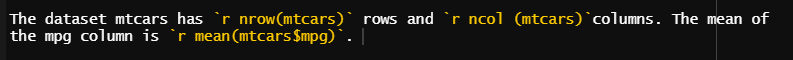
\includegraphics[width=1\linewidth,height=0.45\textheight,]{images/inline_code} \end{center}

\hypertarget{tables}{%
\section{Tables}\label{tables}}

There are a number of packages that make nice tables in R
Markdown. We will use the \texttt{knitr} package for this
example.

The easiest way to make a table in R Markdown is to make a
data.frame with all the data (and column names) you want and
then show that data.frame (there are also packages that can
make tables from regression output though that won't be
covered in this book). For this example we will subset
(which we'll cover in Chapter @ref(subsetting-intro)) the
\emph{mtcars} data (which is included in R) to just the
first 5 rows and columns. The \texttt{kable} function from
the \texttt{knitr} package will then make a nice looking
table. With \texttt{kable} you can add the caption directly
in the \texttt{kable()} function. The option \texttt{echo}
in our code chunk is not set to FALSE here so you can see
the code.

\begin{Shaded}
\begin{Highlighting}[]
\FunctionTok{library}\NormalTok{(knitr)}
\CommentTok{\# Warning: package \textquotesingle{}knitr\textquotesingle{} was built under R version 4.1.3}
\NormalTok{mtcars\_small }\OtherTok{\textless{}{-}}\NormalTok{ mtcars[}\DecValTok{1}\SpecialCharTok{:}\DecValTok{5}\NormalTok{, }\DecValTok{1}\SpecialCharTok{:}\DecValTok{5}\NormalTok{]}
\FunctionTok{kable}\NormalTok{(mtcars\_small, }\AttributeTok{caption =} \StringTok{"This is an example table caption"}\NormalTok{)}
\end{Highlighting}
\end{Shaded}

\begin{table}

\caption{(\#tab:unnamed-chunk-117)This is an example table caption}
\centering
\begin{tabular}[t]{l|r|r|r|r|r}
\hline
  & mpg & cyl & disp & hp & drat\\
\hline
Mazda RX4 & 21.0 & 6 & 160 & 110 & 3.90\\
\hline
Mazda RX4 Wag & 21.0 & 6 & 160 & 110 & 3.90\\
\hline
Datsun 710 & 22.8 & 4 & 108 & 93 & 3.85\\
\hline
Hornet 4 Drive & 21.4 & 6 & 258 & 110 & 3.08\\
\hline
Hornet Sportabout & 18.7 & 8 & 360 & 175 & 3.15\\
\hline
\end{tabular}
\end{table}

For another package to make very nice looking tables, see
\href{https://cran.r-project.org/web/packages/kableExtra/vignettes/awesome_table_in_html.html}{this
guide} to the \texttt{kableExtra} package.

\hypertarget{footnotes}{%
\section{Footnotes}\label{footnotes}}

In your writing, you'll often have sentences that you want
to include but are auxiliary to your main point (or,
frequently, to include links to specific resources such as a
website where you got data from). In these cases you'll want
to include that info as a footnote, which is a section at
the bottom of the page for this kind of information. To
create a footnote in R Markdown, you use the carrot \^{}
followed immediately by square brackets {[}{]}. Put the text
inside of the {[}{]} and it'll print that at the bottom of
the page. Code for a footnote will look like this:
\texttt{\^{}{[}This\ sentence\ will\ be\ printed\ as\ a\ footnote.{]}}.
In cases where you have a very long footnote it may extend
to the next page and will be again at the bottom of the
page. Look down at the bottom of this page to see the
footnote (in a PDF or Word Doc, the footnote will be on the
page you create it on, however since websites are just one
long page without breaks, this footnote is at the very
bottom of this entire page).\footnote{This is an example of
  a footnote.} When you use a footnote, you'll usually put
it immediately after the punctuation of the sentence it
should be after. Note that footnotes are numbered so you can
identify them. There's a blue superscript 1 where we make
the first footnote. If we make another footnote, it'll be
numbered sequentially, such that the next one is 2, the next
is 3, etc.

If you're familiar with LaTeX you can use LaTeX code such as
\texttt{\textbackslash{}footnote\{\}} where the text goes
inside the \{\}. But note that citations (which we'll learn
in Section @ref(citation)) won't work properly in the
footnote if made this way. You can use LaTeX code - and use
LaTeX packages - in R Markdown if you'd like and it'll
operate (in most cases) like normal LaTeX.

\hypertarget{citation}{%
\section{Citation}\label{citation}}

In academic research you will need to cite the papers that
you are referencing. R Markdown has a built-in way to cite
papers, though it's a bit of a process to get everything
setup. You'll need the citation data in BibTeX format and
we'll walk through the steps from finding an article that
you want to cite to citing it in your R Markdown file.
First, a brief overview of what kinds of citations you can
use. There are two types of citations you can use, in-text
and parenthetical. You'll use in-text citations when you
want to have the author names be in the text, and
parenthetical citations when you want everything to be in
parentheses.

Note, there may be other ways to get the citations in the
right format; I'm just showing you one way to do so. For
this example, we'll use the article ``Using NIBRS data to
analyze violent crime'' by Brian Reaves that was published
in 1993. We'll walk through the process from finding the
article on Google Scholar to citing it in your paper. First,
from Google Scholar we'll search for the article title.

\begin{center}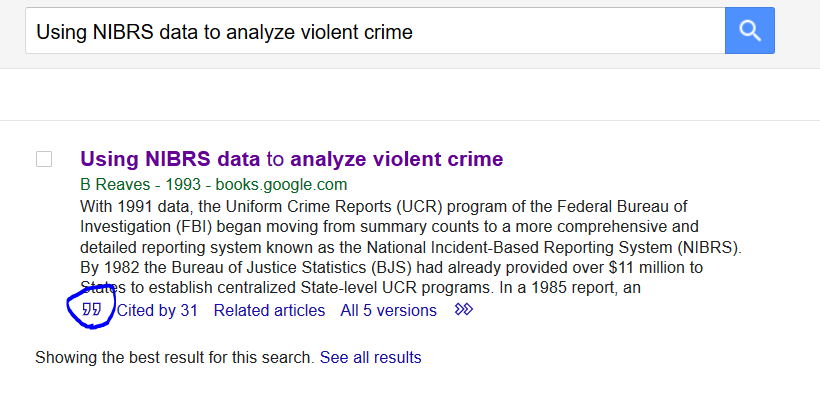
\includegraphics[width=1\linewidth,height=0.45\textheight,]{images/citation_google_scholar} \end{center}

This returns all articles that meet your search criteria.
Since we're searching for a specific article title, we only
get one result. The result shows some basic info about the
article - title, date, name, abstract. Below the abstract
are some important things. First, and circled in blue in the
above photo, is a link that looks like quotation marks. This
is what we'll click on to get to the BibTeX citation. While
not necessary for citation, the next two links may come in
handy during your research. ``Cited by 31'' means that 31
published (in some format that Google can locate, not
necessarily peer-reviewed) articles have cited this article.
If you click the link it'll open up a Google Scholar page
with all of these articles. This is a good way to find
relevant literature. Clicking `Related articles' does the
same thing but with articles that Google Scholar deems
similar, not necessarily articles linking to the one you're
looking up.

But back to the quotes link circled in blue. Click this and
it'll make a popup, shown below, of ways to cite this
article is various formats. We'll have R Markdown
automatically generate the citation in the format we want so
we don't need to worry about this. Instead, click the BibTeX
link at the bottom left.

\begin{center}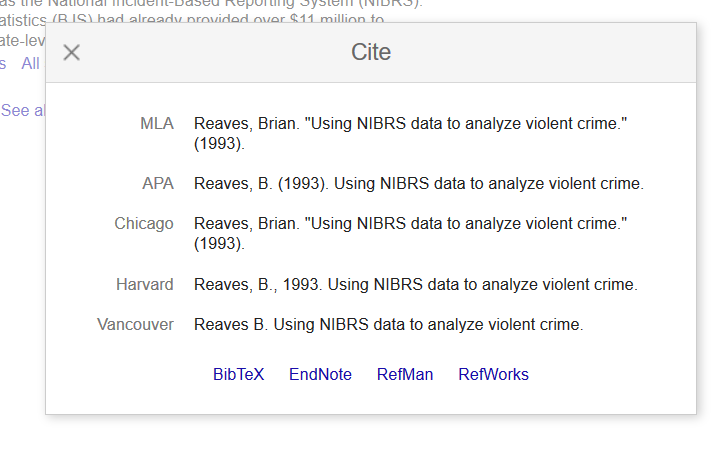
\includegraphics[width=1\linewidth,height=0.45\textheight,]{images/google_scholar_cite} \end{center}

When you click it, it'll open up a new page with that
article's citation in BibTeX form, as shown below. This
basically is just a way to tell a computer how to cite it
properly. Each part of the citation - author, year, title,
etc. - is its own piece. Take a close look at the section
immediately after the first squiggly bracket,
``reaves1993using''. This is how you'll identify the article
in R Markdown so R knows which article to cite. It's
essentially the citation's name. It's created automatically
by combining the author name (first author if there are more
than one author, publication year, and part of the title).
You can change it to whatever you want it to be called.

\begin{center}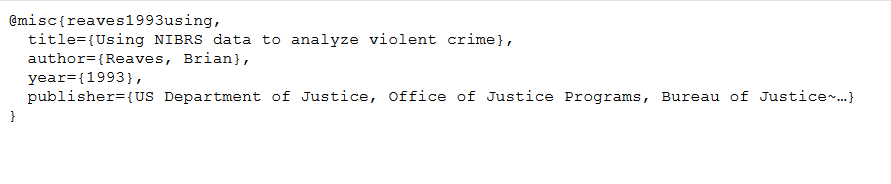
\includegraphics[width=1\linewidth,height=0.45\textheight,]{images/google_scholar_bibtex} \end{center}

Note at the end of the publisher section are the characters
``\textasciitilde\ldots{}''. This looks like a mistake made
by Google Scholar so we'll need to delete that so it isn't
included in a paper we use this citation in. When using
Google Scholar, you'll occasionally find issues like this
which you'll need to fix manually - a bigger issue is
apostrophes or other punctuation may copy over from Google
Scholar weirdly (meaning that it copies as a character that
your computer, and thus R Markdown, doesn't understand) and
needs to be rewritten so R Markdown will run. You can
rewrite it by just deleting the punctuation and typing it
using your keyboard. This isn't always an issue so don't
worry about it unless you get an error with the citations
when outputting your document.

Below is the citation included in my .bib file, and the
start of another citation also included in the file. A .bib
file is basically a text file that programs can read to get
citation info. You'll have all of your citations (in the
BibTeX format) in this one file. To make a .bib file you can
open up a text document, such as through the Notepad app in
Windows, and paste the BibTeX that you've copied from Google
Scholar. Save this file as a .bib extension (by renaming it
filename.bib) and you'll have a usable .bib file.

Note that I have the word NIBRS surrounded by squiggly
brackets \{\}. That is because by default R Markdown (and
other citation generators such as Overleaf) will only
capitalize the first letter of the title or the first letter
following a colon. Since NIBRS is an abbreviation and should
be capitalized, I put it in the \{\} to force it to remain
capitalized. This is often a problem with abbreviations or
country names (such as United States) in the paper title.
Since all citations you use for a project should be in a
single .bib file, you can see the start of another article
citation below the Reaves citation.

\begin{center}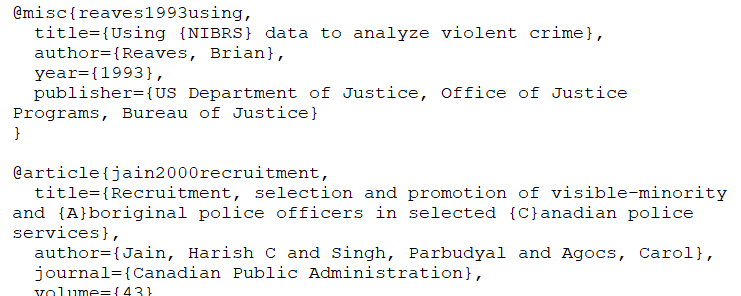
\includegraphics[width=1\linewidth,height=0.45\textheight,]{images/bibtex_example} \end{center}

To use citations from your .bib file, add
\texttt{bibliography:\ references\_file\_name.bib} to the
head of your R Markdown file. If your .bib file isn't in the
R Markdown file's working directory, as my example below is
not, you'll need to include the path in the file name.

\begin{center}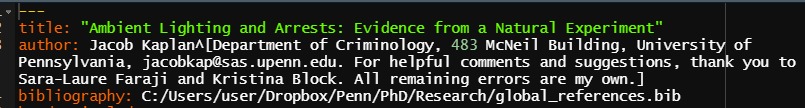
\includegraphics[width=1\linewidth,height=0.45\textheight,]{images/rmarkdown_bib} \end{center}

Now that we have the citation in BibTeX format, have put it
in our .bib file, and have told R Markdown where to look for
that file, we are ready to finally cite that article. To use
a citation we simply put the @ sign in front of the citation
name (in our case ``reaves1993using'') so we would write
\texttt{@reaves1993using}. This will give us an in-text
citation, with the author name in the text and the year in
parentheses. Adding a - right in front of the @ will cause
the citation to show just the year, not the author's name.
You'll usually want to use this if you've already named the
author earlier in the sentence. Generally we will want
parenthetical citations, with both the authors and the year
in parentheses. To do this, we put the citation inside of
square brackets like this \texttt{{[}@reaves1993using{]}}.
If we're citing multiple articles, we separate each citation
using a semicolon
\texttt{{[}@reaves1993using;\ @jain2000recruitment{]}}.

Here's what the results look like when citing that Reaves
article, see the image below for what this looks like just
as code.

\citep{reaves1993using}

\citet{reaves1993using}

-\citet{reaves1993using}

\citeyearpar{reaves1993using}

\citep{reaves1993using, jain2000recruitment}

If you use a citation that isn't in your .bib file, R
Markdown will show a question mark, indicating that you made
some mistake.

\citep{wrongCitation}

\begin{center}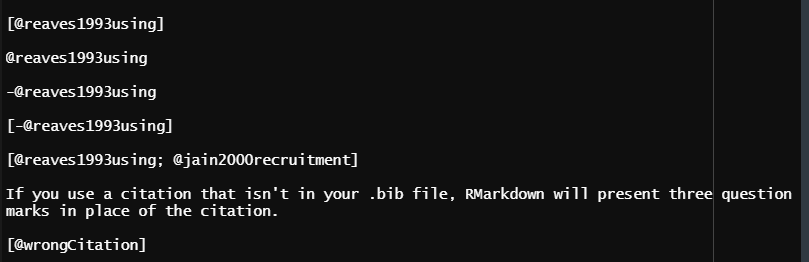
\includegraphics[width=1\linewidth,height=0.45\textheight,]{images/citation_raw} \end{center}

When you use citations, R will automatically put the
reference section at the very end of the document. Two LaTeX
commands may be useful here.
\texttt{\textbackslash{}clearpage} makes a new page so your
reference section isn't on the same page as the conclusion.
\texttt{\textbackslash{}singlespace} makes the reference
section single spaced if your document is set to be double
spaced. Put these commands at the very end of your document
so they only apply to the reference page. You don't need to
do anything other than write them (for easier reading, make
them on separate lines) at the end of the R Markdown file.
If you want to make the references go in another part of the
paper (e.g.~after tables and figures), just put this code at
the place in the paper where you want to reference section
to go:
\texttt{\textless{}div\ id="refs"\textgreater{}\textless{}/div\textgreater{}}.

\hypertarget{spell-check}{%
\section{Spell check}\label{spell-check}}

R Markdown does have a built-in spell checker (the ABC above
a check mark symbol to the left of the Knit button) but it
isn't that great. I recommend that you export to Word (or
open up the PDF in Word if you prefer using PDFs) and using
Word's superior spell checker.

\hypertarget{making-the-output-file}{%
\section{Making the output
file}\label{making-the-output-file}}

To create the Word or PDF output click \texttt{Knit} and it
will create the output in the format set in the very top. To
change this format click the white down-arrow directly to
the right of \texttt{Knit} and it will drop-down a menu with
output options. Click the option you want and it will output
it in that format and change that to the new default.
Sometimes it takes a while for it to output, so be patient.

\begin{center}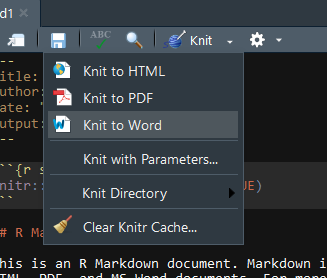
\includegraphics[width=1\linewidth,height=0.45\textheight,]{images/markdown4} \end{center}

\hypertarget{tests}{%
\chapter{Testing your code}\label{tests}}

This chapter covers how to write code that tests other code.
It's especially useful when you write complex functions but
is also useful for work such as PDF scraping or webscraping
where you know the right answer (by looking at the PDF or
webpage yourself) and want to be sure your scraping code did
the scrape correctly. However, in most cases when
programming for research you won't formally test your code -
though you should be checking if everything makes sense and
rereading your code to look out for errors (such as typos or
using the wrong data). If you've never programmed before, I
recommend that you skip this chapter entirely (or read it
but don't feel pressure to understand everything) and return
to it after you've finished the rest of the book.

\hypertarget{why-test-your-code}{%
\section{Why test your code?}\label{why-test-your-code}}

As you write code, you will inevitably make mistakes. There
are two main types of mistakes with coding - those that
prevent code from working (i.e.~give you an error message
and don't run the code) and those that run the code but give
you the wrong result. Of these, the first is probably more
frustrating as R tends to give fairly unhelpful error
messages and you'll feel you hit a roadblock since R just
isn't working right. However, the second issue - code is
wrong but doesn't tell you it's wrong! - is far more
dangerous. This is especially true for research projects.

Let's use examining whether a policy affected murder as an
example. In the example data set below, we have two years of
data for both murder and theft, and we'll say that the
policy changed at the start of the second year. If we want
to see if murder changed from 2000 to 2001, we could (overly
simply) see if the number of murders in 2001 was different
from the number in 2000. And since the data also has theft,
we'd want to subset to murder first.

\begin{Shaded}
\begin{Highlighting}[]
\NormalTok{example\_data }\OtherTok{\textless{}{-}} \FunctionTok{data.frame}\NormalTok{(}
  \AttributeTok{year =} \FunctionTok{c}\NormalTok{(}\DecValTok{2000}\NormalTok{, }\DecValTok{2000}\NormalTok{, }\DecValTok{2001}\NormalTok{, }\DecValTok{2001}\NormalTok{),}
  \AttributeTok{crime\_type =} \FunctionTok{c}\NormalTok{(}\StringTok{"murder"}\NormalTok{, }\StringTok{"theft"}\NormalTok{, }\StringTok{"murder"}\NormalTok{, }\StringTok{"theft"}\NormalTok{),}
  \AttributeTok{crime\_count =} \FunctionTok{c}\NormalTok{(}\DecValTok{100}\NormalTok{, }\DecValTok{100}\NormalTok{, }\DecValTok{200}\NormalTok{, }\DecValTok{50}\NormalTok{)}
\NormalTok{)}
\NormalTok{example\_data}
\CommentTok{\#   year crime\_type crime\_count}
\CommentTok{\# 1 2000     murder         100}
\CommentTok{\# 2 2000      theft         100}
\CommentTok{\# 3 2001     murder         200}
\CommentTok{\# 4 2001      theft          50}
\end{Highlighting}
\end{Shaded}

To see if murder changed, we can subset to the rows where
the crime is murder, and then print out the year and
crime\_count columns to see if there is a change. So our
code will be
\texttt{example\_data{[}example\_data\$crime\_type\ ==\ "murder",\ c("year",\ "crime\_count"){]}}.
Below I've accidentally only put one \texttt{=} instead of
two, this will give us an error and not give any other
results. Helpfully, the error message tells us that there's
an error with the \texttt{=} sign, though not what that
exact error is.

\begin{Shaded}
\begin{Highlighting}[]
\NormalTok{example\_data[example\_data}\SpecialCharTok{$}\NormalTok{crime\_type }\OtherTok{=} \StringTok{"murder"}\NormalTok{, }\FunctionTok{c}\NormalTok{(}\StringTok{"year"}\NormalTok{, }\StringTok{"crime\_count"}\NormalTok{)]}
\CommentTok{\# Error: \textless{}text\textgreater{}:1:38: unexpected \textquotesingle{}=\textquotesingle{}}
\CommentTok{\# 1: example\_data[example\_data$crime\_type =}
\CommentTok{\#                                          \^{}}
\end{Highlighting}
\end{Shaded}

Now I've made a different mistake. Here, instead of
\texttt{==}, I've written \texttt{!=} which is the opposite
of what we want - it'll return all rows that do \textbf{not}
equal ``murder''. Now it looks like the policy cut murder in
half when in actuality the policy doubled murders! Since we
don't print out the type of crime in the output, we wouldn't
catch this from the output alone.

\begin{Shaded}
\begin{Highlighting}[]
\NormalTok{example\_data[example\_data}\SpecialCharTok{$}\NormalTok{crime\_type }\SpecialCharTok{!=} \StringTok{"murder"}\NormalTok{, }\FunctionTok{c}\NormalTok{(}\StringTok{"year"}\NormalTok{, }\StringTok{"crime\_count"}\NormalTok{)]}
\CommentTok{\#   year crime\_count}
\CommentTok{\# 2 2000         100}
\CommentTok{\# 4 2001          50}
\end{Highlighting}
\end{Shaded}

You may think this is a silly example that is unrealistic.
And it is to a degree, it's just one line of code that we're
using to evaluate an entire policy. Now think about how you
would actually evaluate a policy using data that you're
familiar with. Now the code is going to be much more
complex. Your code may be hundreds of lines long, deal with
multiple data sets that must be joined together, and involve
a number of relative subjective (though must be defensible)
decisions as to how to deal with your data (e.g.~what crimes
constitute violent crime, what time unit to analyze), and
some of the code may be written by other people who you are
collaborating with. The increased complexity with a real
analysis increases the likelihood that errors will occur -
and even small issues such as an incorrect subset can have
large impacts on your results.

So, how do we properly test our code? There are two main
methods that I'll refer to as informally testing and
formally testing. The formal method will be using something
called ``unit tests'' that we'll discuss in the next part of
this chapter.

Informal methods are what you've likely been doing already.
Essentially, just looking at your data and trying to see if
it ``looks right''. This includes stuff like printing
summary statistics (using \texttt{summary()}) of important
variables and making simple graphs to look at the data. If
something is wrong, exploring the data is a fairly good way
to discover it. For example, if you are looking at arson
data from the FBI, you may find (as this is actually in the
data) some cities with millions of car arsons in a month.
This is clearly wrong so you know there's an issue - in this
case, an issue with not subsetting out obvious outliers.
Knowledge about the topic and the data are also important in
this approach. If you are familiar with a given topic and
your results are similar to that of past studies, that's a
good sign that you did things right.\footnote{However, make
  sure that you don't look less closely just because the
  results are the way you expect. Past results may be wrong,
  or you can have a new finding, so make sure to avoid
  complacency just because you like the results}

You can also take this kind of approach when testing
functions - which ideally are the way you write code. For
example, if you have a function that takes a number and
returns that number + 2, you can test it by checking a few
cases. If you input 2, you expect 4. If you input -2, you
expect 0. Do this a few times and you can be more confident
that the function works properly. Now imagine a function
that's more complex - one that calls a different function
and uses the result of that function. If you change the
underlying function, you'll need to check both that function
and the function that calls it.

As you have more intertwined pieces in your code, this gets
more and more complex. It also takes a lot more time as
you'll have a lot of code that only checks a function and
will have to run it line by line to see if there's an issue.
At this point, relying on informal methods becomes
unfeasible and you'll want to use unit tests, a formal way
to test your code. Note, however, that this is far better
suited for checking functions than for checking data, though
it is possible to some degree. We'll discuss formally
testing data in Section @ref(tests-for-research-projects).

\hypertarget{unit-tests}{%
\section{Unit tests}\label{unit-tests}}

A unit test is simply a conditional statement where you have
some input, usually a function with some parameters set, and
state what you expect the result to be. You are saying ``I
expect that if I do X, I will get Y''. And if you get a
result other than what you expected, R will tell you. In R,
you can make a number of unit tests and have R run them all
at once and inform you of which ones failed. Each unit test
is just a function in R that is specifically for checking
whether other functions - or other code or data - are
correct. They operate just like a normal function. To use
unit tests, we'll use the R package \texttt{testthat} which
has a number of functions that make unit testing easier, and
we'll use some keyboard shortcuts in RStudio that also
improve the ease of testing.

Please note that these shortcuts will only work if you're
working in an R Package, a normal R Project won't work. An R
Package is a special type of R Project, which you can make
by following the steps in Section @ref(r-projects) and
choosing ``R Package'' instead of ``New Project'' in the
Project Type panel. An R Package is essentially an R Project
with the goal of creating a package in R, though there's no
requirement that we actually make a package. We can treat it
as a normal R Project but use the added testing tools.

If you don't have \texttt{testthat} installed, do so using
\texttt{install.packages("testthat")}. For more information
on the package, please see the package's
\href{https://testthat.r-lib.org/index.html}{website}.

\begin{Shaded}
\begin{Highlighting}[]
\FunctionTok{install.packages}\NormalTok{(}\StringTok{"testthat"}\NormalTok{)}
\end{Highlighting}
\end{Shaded}

\begin{Shaded}
\begin{Highlighting}[]
\FunctionTok{library}\NormalTok{(testthat)}
\CommentTok{\# Warning: package \textquotesingle{}testthat\textquotesingle{} was built under R version 4.1.3}
\CommentTok{\# }
\CommentTok{\# Attaching package: \textquotesingle{}testthat\textquotesingle{}}
\CommentTok{\# The following object is masked from \textquotesingle{}package:tidyr\textquotesingle{}:}
\CommentTok{\# }
\CommentTok{\#     matches}
\CommentTok{\# The following object is masked from \textquotesingle{}package:dplyr\textquotesingle{}:}
\CommentTok{\# }
\CommentTok{\#     matches}
\CommentTok{\# The following objects are masked from \textquotesingle{}package:readr\textquotesingle{}:}
\CommentTok{\# }
\CommentTok{\#     edition\_get, local\_edition}
\end{Highlighting}
\end{Shaded}

In \texttt{testthat}, every function follows the same
\texttt{expect\_} format where a type of conditional
statement follows the \_. For example,
\texttt{expect\_equal()} checks if two values are equal,
\texttt{expect\_named()} checks if the name of a data set is
correct, and \texttt{expect\_silent()} makes sure that the
code that's run doesn't return any warnings, messages, or
errors. To use this technique for our above example of the
function that adds 2 to an inputted number - which we'll
call \texttt{add\_2()} - we can use some
\texttt{expect\_equal()} functions. If we input 2, we expect
4. So we'd write \texttt{expect\_that(add\_2(2),\ 4)}.

\begin{Shaded}
\begin{Highlighting}[]
\NormalTok{add\_2 }\OtherTok{\textless{}{-}} \ControlFlowTok{function}\NormalTok{(number) \{}
  \FunctionTok{return}\NormalTok{(number }\SpecialCharTok{+} \DecValTok{2}\NormalTok{)}
\NormalTok{\}}
\FunctionTok{expect\_equal}\NormalTok{(}\FunctionTok{add\_2}\NormalTok{(}\DecValTok{2}\NormalTok{), }\DecValTok{4}\NormalTok{)}
\end{Highlighting}
\end{Shaded}

Above is the code that makes the \texttt{add\_2()} function
and one unit test checking it. It doesn't output anything.
That is good. When a test passes, there is no information;
when it fails, the function will output a message that it
failed. Below is another test, this one intentionally wrong
to show what happens when a test fails.

\begin{Shaded}
\begin{Highlighting}[]
\FunctionTok{expect\_equal}\NormalTok{(}\FunctionTok{add\_2}\NormalTok{(}\DecValTok{2}\NormalTok{), }\DecValTok{5}\NormalTok{)}
\CommentTok{\# Error: add\_2(2) not equal to 5.}
\CommentTok{\# 1/1 mismatches}
\CommentTok{\# [1] 4 {-} 5 == {-}1}
\end{Highlighting}
\end{Shaded}

It gives an error, telling us that the result of the
\texttt{add\_2(2)} function does not equal 5. Helpfully, it
also shows us how much of a difference there is between what
we expected and what we got. Note that it says ``1/1
mismatches''. That says that all of the expected values - we
only expect one value here - are incorrect. If we expect
more than one result, such as if we expect a function to
return a vector, it will check each value and say exactly
which ones (in the order we have the resulting vector) are
incorrect. This is helpful when diagnosing exactly which
part failed.

There are a few different ways to run the unit tests. First,
you can run them like a normal R script by running each line
directly. This is fairly inefficient and loses some of the
benefits built into RStudio for testing. Though in this case
you do \textbf{not} need to be using an R Package, you can
just use a normal R Project or just use normal R and the
code will work fine.

The next way is to use the \texttt{test\_dir()} function
from the \texttt{testthat} package where you enter the
folder directory in the parentheses and it runs every test
file in that folder. It's easier to simply use the
\texttt{test\_path()} function which inserts the correct
folder, assuming that you didn't move folders around after
\texttt{use\_test()} (which we'll discuss below) created
them. So you'd write \texttt{test\_dir(test\_path())} and it
would run all of your tests. This also prints out a nice
summary of the results for all of your tests combined,
showing the number of tests that passed, that failed
(i.e.~didn't pass), that returned warnings, and that were
skipped (you can force R to skip some tests which is useful
when you change one part of the code and know those tests
will fail but still want to test other parts).

You will also need to run all the functions or load all of
the data that the tests check, otherwise you'll get an error
since R doesn't implicitly know that the functions/data
exist. You can run this the normal way by highlighting and
running the function (or the code to load data) in your R
script or use the shortcut Control+Shift+L (Command+Shift+L
on a Mac, the L stands for ``Load'') which will run every R
file in your project (and every line of each file).

The final way is to use the keyboard shortcut
Control+Shift+T (Command+Shift+T on a Mac, the T stands for
``Test'') which will load all of the files in your folder
and then run all of the tests. It's a quicker way of doing
the above method. However, this shortcut only works when
using an R Package, not a normal R Project.

\begin{center}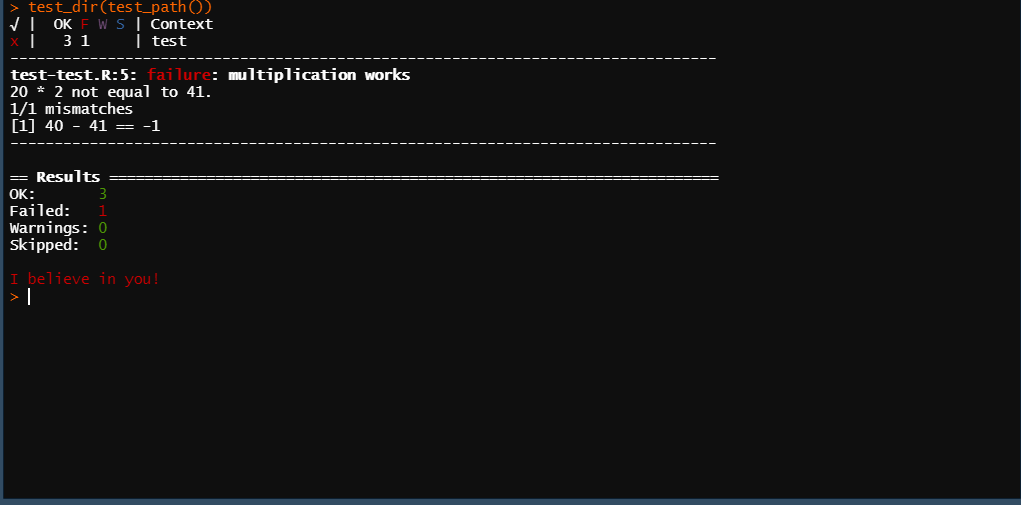
\includegraphics[width=1\linewidth,height=0.45\textheight,]{images/test_summary} \end{center}

\hypertarget{modular-test-scripts}{%
\subsection{Modular test
scripts}\label{modular-test-scripts}}

Before getting into exactly how to write a unit test
correctly, we'll talk about organizing each testing file. As
with your normal R script, you can have separate testing
scripts (a testing script is a normal R script which people
use specifically for testing code but doesn't actually
function any different) for each major part of the code that
you're testing.\footnote{For more info on having separate R
  scripts for each major section of your code, please refer
  to Section @ref(modular-r-scripts)} As with the R scripts
for your code, this is simply a way to organize your work,
and doesn't affect the testing. Below is an image showing
the files I use to test the US Border Patrol scrapers. I
have one file per PDF that I scraped.

\begin{center}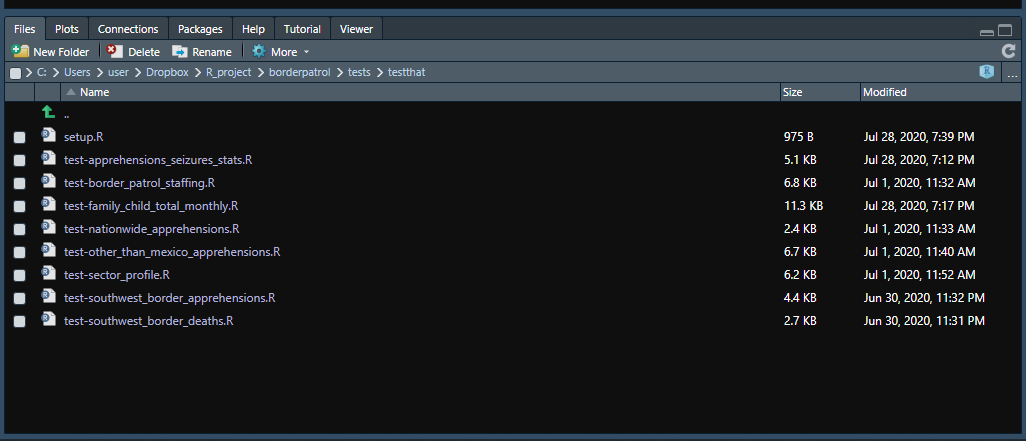
\includegraphics[width=1\linewidth,height=0.45\textheight,]{images/test_file_setup} \end{center}

Note where the folder depicted above is located. It's in a
folder called ``testthat'' in the ``tests'' folder in the
main project folder that I called ``borderpatrol.'' We'll
use a helpful function from the \texttt{usethis} package to
organize our test files and generate them automatically. If
you haven't installed this package already, do so using
\texttt{install.packages("usethis")} and then load it with
\texttt{library(usethis)}. \footnote{The \texttt{usethis}
  package is an extremely helpful package that automates a
  lot of work that you would do primarily for R package
  development so if you go down that route I recommend
  exploring the package more through its website
  \url{https://usethis.r-lib.org/index.html}).}

You can use the function \texttt{use\_test()} from the
\texttt{usethis} package to create a test file inside your R
Project. This will automatically create the necessary file
and folders (if not created already) so you don't have to do
any more work. Run this function by putting the name of the
test file you want to create (in quotes) in the parentheses.
It will open the test file in the Source panel (shown in the
top left). In the example shown below, I wrote
\texttt{use\_test("test")} to make a new file called
``test''. In the Source panel, the file is called
``test-test.R,'' which is just because \texttt{usethis} will
automatically add ``test-'' to the name of any test file
name you make. \texttt{use\_test()} will also generate an
example of a test, which you can modify (or delete entirely)
to suit your own needs.

\begin{center}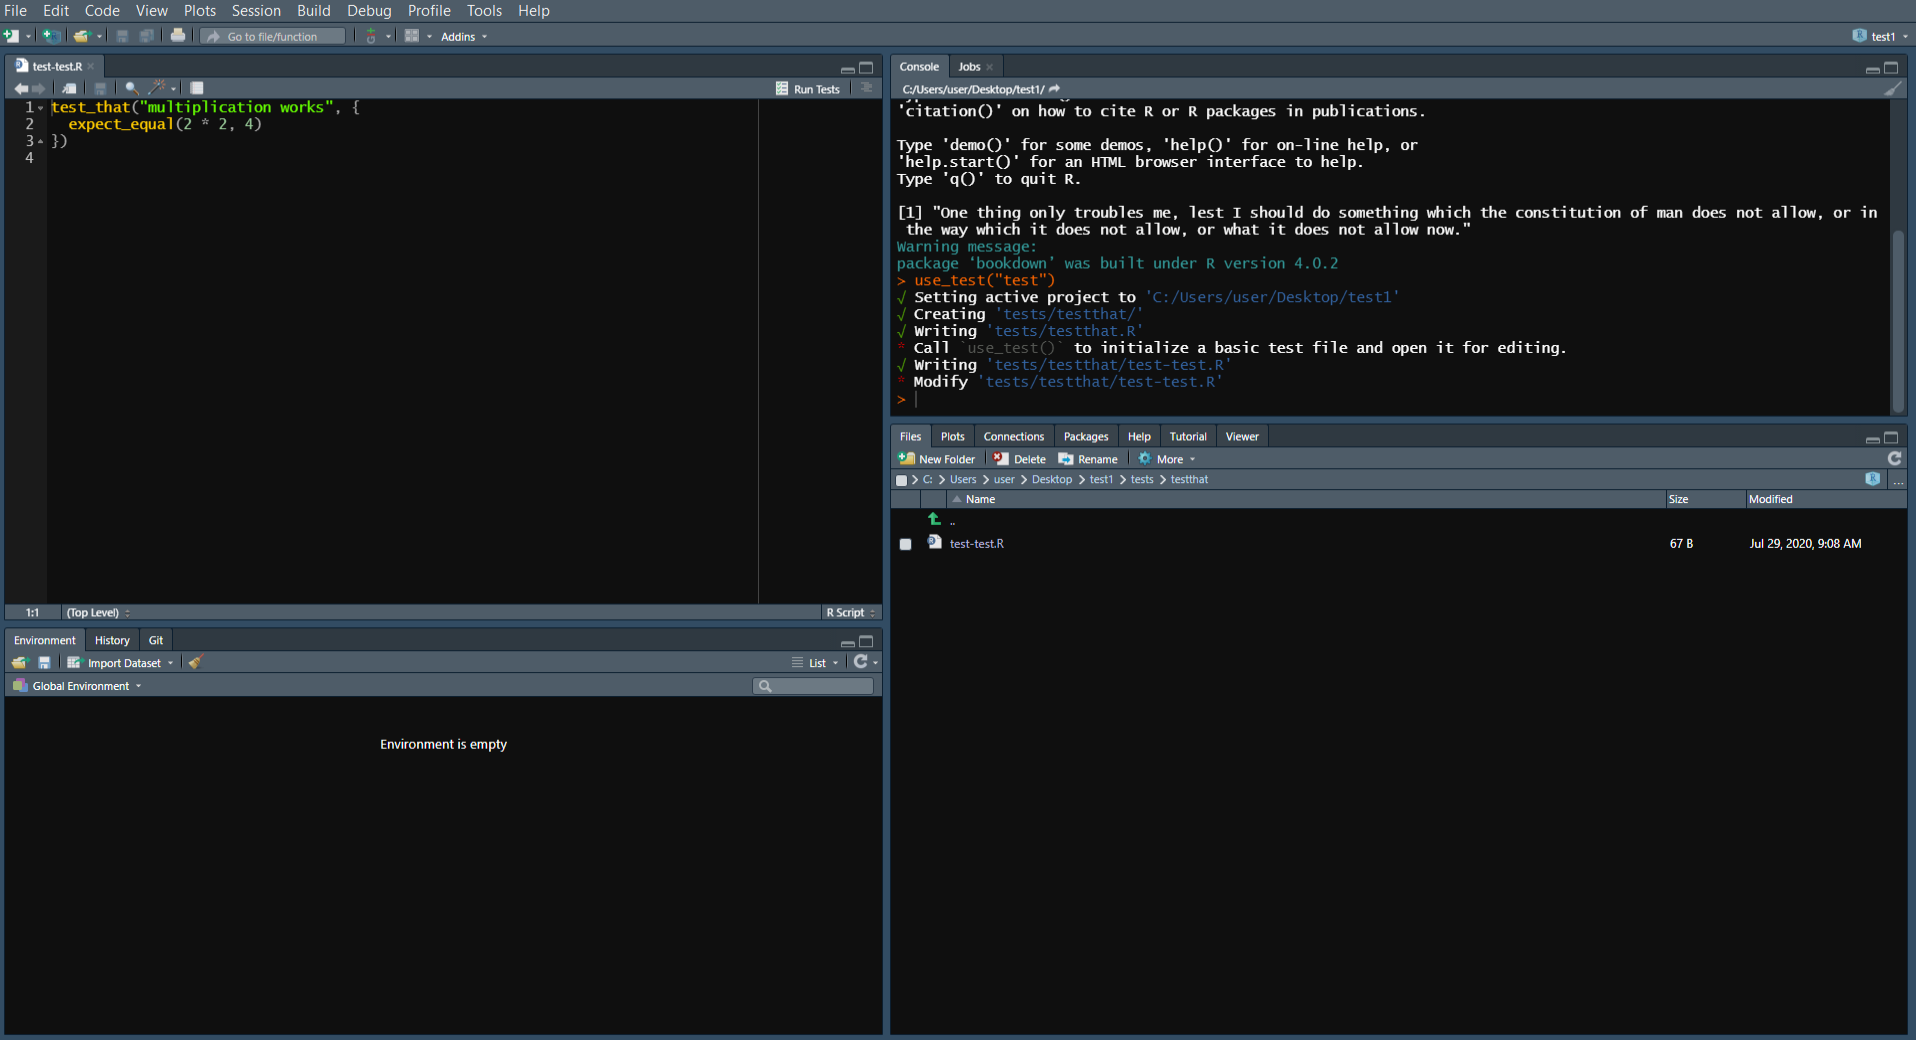
\includegraphics[width=1\linewidth,height=0.45\textheight,]{images/usethis_test} \end{center}

The first file in the testthat folder is called setup.R,
which is a file that will automatically run first when you
run a test script through R or using RStudio's keyboard
shortcut. This file is where you run some code that is used
during the tests. In my setup.R file I made several vectors,
which I use during the tests to subset the data. You won't
always need to have a setup.R file, but it's useful when you
want to run the same code beforehand for multiple different
test scripts.

\begin{center}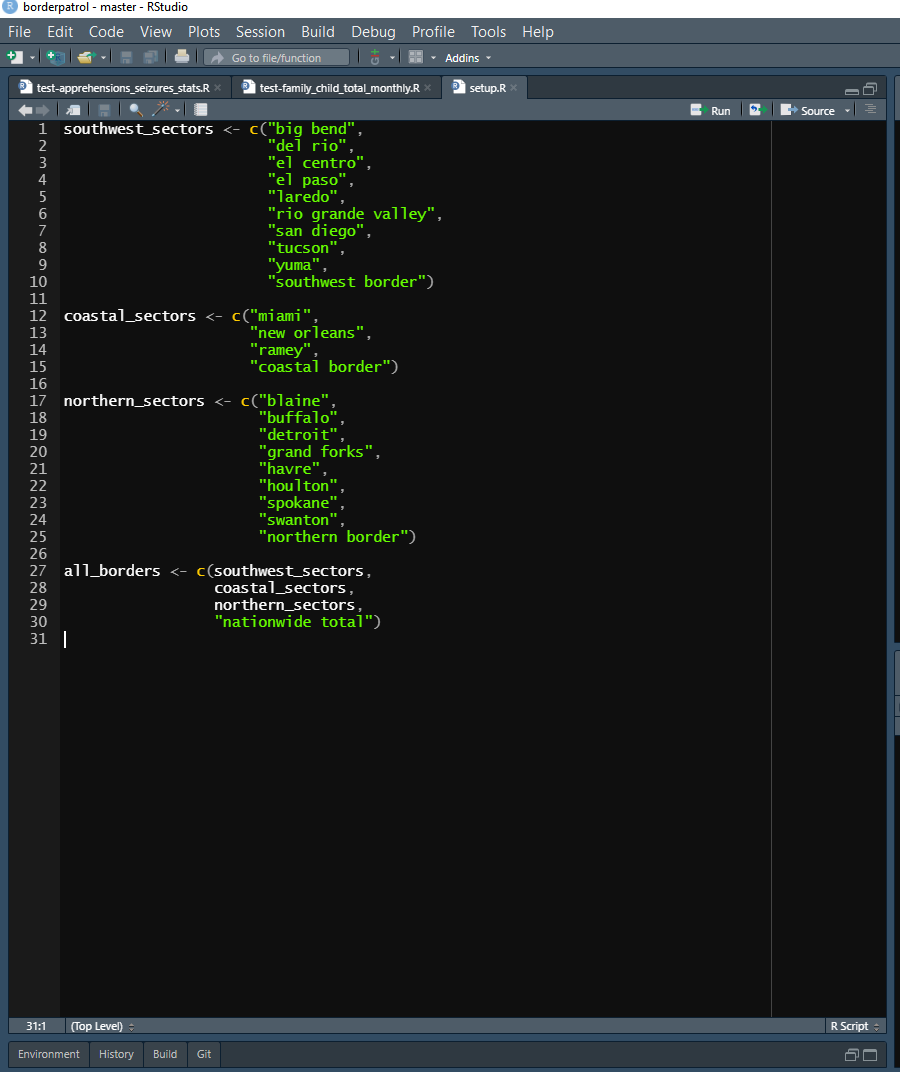
\includegraphics[width=1\linewidth,height=0.45\textheight,]{images/test_setup} \end{center}

\hypertarget{how-to-write-unit-tests}{%
\subsection{How to write unit
tests}\label{how-to-write-unit-tests}}

We'll start by looking at the default test example made when
using \texttt{use\_test()} to understand the organization of
a test file before getting into an example of actual tests.
In the image below, there are really two pieces. First, we
have the actual test on line 2 -
\texttt{expect\_equal(2\ *\ 2,\ 4)}. This is saying, I
expect 2 * 2 to equal 4, and R will check if that is true.
All of your tests will be in this format, just for a
specific result from a specific input. Now let's look at the
code surrounding that line -
\texttt{test\_that("multiplication\ works",\ \{\})} where
the \texttt{expect\_equal()} line goes inside the \{\}.

\begin{center}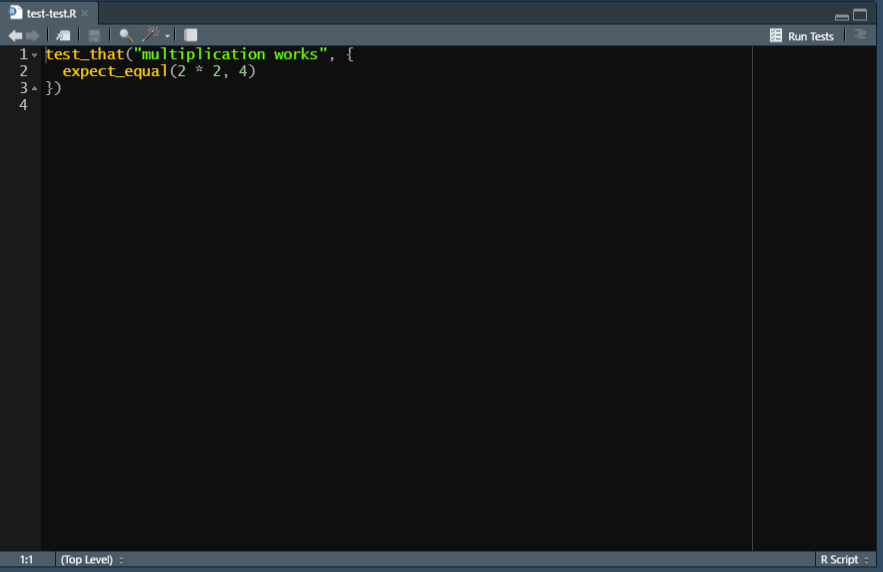
\includegraphics[width=1\linewidth,height=0.45\textheight,]{images/usethis_test_default_example} \end{center}

The \texttt{test\_that} code is basically a form of
organization within a test file to group similar tests
together. In this case it is grouping all of the tests that
check if ``multiplication works,'' though we only have one
test written. Below I've added three new tests to this
``multiplication works'' testing group. To run this code, I
can either run each \texttt{expect\_equal()} individually
(remember to run \texttt{library(testthat)} beforehand or it
won't run) or run the entire \texttt{test\_that()} group at
once. You can do this by either highlighting it all and
running it or selecting either the top or bottom line (which
has the squiggly brackets) and running that line - the
entire thing will run.

The benefit of this is that when you run all the tests you
write (and you'll often have many test groups and more
individual tests than shown here), if a test in a group
fails, it will tell you exactly which group failed (based on
the name of the group which you specify - here,
``multiplication works''). Note that the final test in this
example is incorrect, and in the Console panel on the right
it says that ``Test failed: `multiplication works' to tell
you where the test failed. The test groups aren't necessary,
but they make it easier to organize your tests.

\begin{center}\includegraphics[width=1\linewidth,height=0.45\textheight,]{images/usethis_test_default_example2} \end{center}

As an example of actual tests, we'll go over the tests that
I wrote when I first scraped the US Border Patrol data that
we will scrape in Chapter @ref(scrape-table). This test file
is organized almost identically to the example one shown
above. At the start I have some code that loads the data
that I will test - this isn't in the setup file since the
code is for this specific test script (though it could be in
the setup.R file and the results would be the same). While
most tests check the result of functions, here I am checking
the data that is outputted by the function, and not
rerunning the function for each test. I do this because the
function that scrapes the PDF is relatively slow to run and
I have many tests, but putting the function that gets the
data in the test directly will give the exact same results.
Then there are several \texttt{test\_that()} groups with
some \texttt{expect\_equal()} tests inside each.

Since these tests are checking if the code is scraping the
PDFs correctly, I determine the expected result by looking
at the PDFs and writing down what the values should be (be
careful, this must be done by hand but that can mean you
mistype - so double-check your work!). We'll use the test on
lines 21-22 as an example. Here I am asking if the values in
the ``cocaine\_pounds'' column, for rows where the sector is
``coastal border'' are equal to the values
\texttt{c(6843,\ 1701,\ 3169,\ 1288,\ 6884,\ 20,\ 709,\ 5962,\ 989)}.
If they are, then the scraping was correct (at least for
this part of the PDF) and the code worked. In this case I
checked every value that meets the two conditions, but
that's just because there were relatively few values. If I
had many values that meet those conditions (i.e.~many rows
of data in that column), I would just check a small number
of them.

\begin{center}\includegraphics[width=1\linewidth,height=0.45\textheight,]{images/test_example} \end{center}

\hypertarget{what-to-test}{%
\subsection{What to test}\label{what-to-test}}

Now that we've gone over how to make unit tests, let's talk
about what to test. When testing functions, you generally
want to test every possible parameter in the function, and a
variety of inputs. In particular, try to think of ways that
the function could be used incorrectly and write a test to
catch that. For example, our \texttt{add\_2()} function will
fail if a string (e.g.~``2'') was inputted instead of a
number, so you'll want to add a test for that. You'll also
want to make sure that inputting something other than simply
a single number, such as a vector of numbers, works as
expected. Basically, you want to be thorough and cover all
of your bases.

Writing unit tests is one of the most time-efficient things
you can do since it helps you avoid making costly (in time
and in getting wrong results) mistakes. But don't spend too
much time writing tests. If you've tested that
\texttt{add\_2(2)} equals 4, no need to test that
\texttt{add\_2(3)} equals five since you're essentially
testing the exact same thing. And consider your audience
(even if that is only you). If you know that
\texttt{add\_2()} will only be used by people who know
better than to input a string, there's no need to test for
that. In general, I think it's always better to have more
tests than fewer, but consider whether writing that test is
a good use of your time. This is something that you'll learn
with experience so it's better to have too many tests when
you're first using R than too few.

\hypertarget{tests-for-research-projects}{%
\subsubsection{Tests for research
projects}\label{tests-for-research-projects}}

When you use R for a research project, you'll usually take
data that someone else collected, or scrape it yourself, do
some work to clean this data (e.g.~subset or aggregate the
data, standardize values) and then run a regression on it.
In these cases there are relatively few opportunities to use
unit tests to check your code. Indeed, the best checks are
often content knowledge about the data and examining the
results of your analysis to see if it makes sense and fits
prior literature.

While testing is most commonly used for functions, you can
use it to test data. Writing tests for research data is best
if your code is scraping the data (webscrape or PDF scrape)
and you want to verify that it is correct, or if you expect
the data to change and want to ensure that it is still
correct (while exact values will change, you can check broad
categories such as whether certain groups are included). For
example, if you know that you only want to look at a certain
state, you can write a test that expects the only state in
the data to be the one you're analyzing. This way, if you
add more data, such as a new release of that data set, the
test will catch if there's any other state that you may have
forgotten to remove after adding the new data. If you're
sure that you will only use a particular data set that never
changes, you're better off just writing code in your main R
script (or a specific script for checking the data) to do
these checks rather than dedicated tests.

\hypertarget{tests-for-data-collection}{%
\subsubsection{Tests for data
collection}\label{tests-for-data-collection}}

Our example in this chapter was tests for a data collection
process - in our case, PDF scraping - so we've already seen
how to test code for gathering data. We'll still talk
briefly here about what kind of tests - and how many tests -
you will want for this type of code. In normal tests, you
don't want to test the exact same thing multiple times (for
example, if you test that 2 + 2 = 4, you don't need to test
that 2 + 3 = 5). This is different when it comes to testing
code that collects data from a source, such as through PDF
scraping or webscraping.

When testing data collection code, you want to be far more
thorough, retesting something in multiple ways. This is
because small differences in the data you are scraping may
affect the code at different parts of the scrape. For
example, imagine a PDF with ten pages and a single table on
each page. On the first page there five columns but on the
next nine pages there are six columns. If you test only data
from the first page you'll miss all of the pages where there
are six columns instead of five - and where your code to
scrape it is probably wrong.

I've often experienced PDF or webscraping where some parts
of the data are just ``weird'' and cause the code to scrape
it incorrectly - but often not tell me that there's an
issue. So to catch this you'll need far more tests than
normal. I prefer to choose a few random pages (more if the
PDF/website is longer) and test random rows and columns
since that'll give a good coverage of the results. In
addition, I look at the PDF or website and try to see if
there's anything atypical about a certain part; if there is,
I test that specifically. It's easy to over-test (and that's
better than under-testing) this kind of work, but there are
rapidly diminishing returns. So test comprehensively but not
at the cost of having too little time to work on code -
again, this is something that requires experience and
doesn't have a hard rule on what constitutes too much (or
too little) testing.

\hypertarget{test-driven-development-tdd}{%
\section{Test-driven development
(TDD)}\label{test-driven-development-tdd}}

We'll finish this chapter by talking about test-driven
development (TDD), a philosophy in programming where you
write the tests first and then write the code that meets
these tests after. This is really an extension to the
discussion in Chapter @ref(mise-en-place) of planning out
your project before you start. In Chapter
@ref(mise-en-place) we talked about writing out every step
of the project and hand sketching all the figures or tables
that you intended to have. With TDD, you write tests for all
of the functions you intend to write (and any variations of
parameters or inputs for these functions) or data you intend
to gather/clean.

Test-driven development is a useful tool to make you really
think about the functions that you need to write, and how
they interact with each other. This is an excellent way to
identify potential issues (I've often realized while writing
tests that the approach I was going to do wouldn't work)
before you start on the code. However, for this same reason,
it is a fairly advanced topic since you need to know exactly
(or, mostly) what you need to do, and the likely problems
that each approach will face. For that reason, I recommend
holding off on using TDD until you're fairly experienced
with R or programming in general.

\hypertarget{git}{%
\chapter{Git}\label{git}}

This chapter covers Git, which is a way to have version
control for your code - like a programming version of
Dropbox, but with a few added features. This is relatively
advanced material and isn't necessary for using R. However,
when you're dealing with complex projects or with multiple
collaborators it is helpful to use. Given that this material
is relatively advanced, feel free to skim or skip this
chapter entirely, and come back to it when you think you
need it - which will likely be after you finish the rest of
the book.

\hypertarget{what-is-git-and-why-do-i-need-it}{%
\section{What is Git, and why do I need
it?}\label{what-is-git-and-why-do-i-need-it}}

As you write R code you will - I hope! - save your R script
from time to time to avoid losing any code you've written if
you close R or shut down your computer. This is important as
it'll save everything you've done locally, but if your
computer crashes you'll want your work to be backed up
elsewhere. While you should have something like Dropbox or
Google Drive that keeps backups of your work, here we'll
talk about Git, which is a version control software that
gives you much more control (but requires more work) of the
saved work than from something like Dropbox.\footnote{This
  came in handy for me as somehow one of my dissertation
  papers written in R Markdown became empty a couple of
  months before my defense, and I couldn't undo that change.
  My Dropbox backup was older than my Git backup so having
  Git was a real time-saver.}

Before getting into exactly how to use Git, we'll talk first
about what it is and how it'll help your work. Git is also a
very powerful and complex tool so this guide is going to be
touching just a small - but useful to most researchers and R
programmers - part of it.

With backup software such as Dropbox, it'll save your work
very frequently - so frequently in fact that I sometimes
turn off Dropbox when I write R since it keeps interrupting
me by saving at the moment I'm typing, which stops the
typing. The following image is the Dropbox page for some R
code that I've been working on to scrape Covid data. Notice
the timestamps - 4/5 of them are within one minute, showing
how often Dropbox is saving changes. This is useful if I
need the most recent update - or to share the most recent
version with a collaborator. Here's the big issue - and the
one that Git solves - I have four versions within a minute
of each other: what's the difference between them? Dropbox
is saving automatically and doesn't indicate how they're
different (clicking on the file shows the complete file, not
differences relative to some previous version), which means
if I mess up some code a while ago, I can't easily see which
version is the one that works. With Git you can wait until
you've made enough changes to decide that these changes
merit a new ``version'' of your work.

\begin{center}\includegraphics[width=1\linewidth,height=0.45\textheight,]{images/dropbox} \end{center}

If you've ever used the track changes feature on a Word
Document, the concept is similar. When you have this setting
in a Word Document every time you (or anyone else) makes
changes in that document, those changes, who made them, and
when they occurred, is tracked. This makes it easy to see
exactly what part of the file was changed and to undo that
change if necessary. Below is an example of this feature on
one of my drafts on Overleaf (basically a way to collaborate
using LaTeX, which is similar to R Markdown). You can see
each change that my co-author made in the draft in the
purple changes in the main part of the photo. The parts that
were rewritten or added are highlighted in purple while the
parts that were deleted are crossed out. What is shown in
purple isn't all of the history of changes for this paper.
If you look at the part on the right, highlighted in green,
it shows what files were edited, by whom, and at what time.
If you don't like a change - or in R's case more commonly,
broke some code by accident - you can go back in the history
of changes and return to an older version.

\begin{center}\includegraphics[width=1\linewidth,height=0.45\textheight,]{images/overleaf} \end{center}

The way that R - and many other programming languages (and
technically you can use this for any file or folder) does
this ``version control'' is through Git.

\hypertarget{git-basics}{%
\section{Git basics}\label{git-basics}}

There are four main processes you need to know for a basic
understanding of Git: checkout, add and commit, push, and
pull. This chapter will explain how to use Git through
buttons on RStudio so you don't necessarily need to know
these commands in Git, but it's useful to know enough to
talk about them and ask questions if needed.

We'll use the example of getting a book from the library to
walk through using Git. The steps for this are simple, we go
to the library, pick a book we want, check it out from the
librarian, read it, and eventually return it. Using Git adds
one wrinkle to this: we will want to write in the book and
see what other people write too. Of course, when the book is
checked out, no one else could write in our version, and no
one can see what we write. So anything we write has to be
done before we return the book to the library, then we check
out the book again to see what other people have written.
When we want another book, we simply redo these steps.

\begin{longtable}[]{@{}
  >{\raggedright\arraybackslash}p{(\columnwidth - 4\tabcolsep) * \real{0.3333}}
  >{\raggedright\arraybackslash}p{(\columnwidth - 4\tabcolsep) * \real{0.3333}}
  >{\raggedright\arraybackslash}p{(\columnwidth - 4\tabcolsep) * \real{0.3333}}@{}}
\toprule()
\begin{minipage}[b]{\linewidth}\raggedright
Library Steps
\end{minipage} & \begin{minipage}[b]{\linewidth}\raggedright
Git steps
\end{minipage} & \begin{minipage}[b]{\linewidth}\raggedright
Git code
\end{minipage} \\
\midrule()
\endhead
Go to library & & \\
Find book and check out book & Clone (usually will just be
done once per project). & Git clone \emph{path to repo, can
be GitHub link} \\
Read or write in book & This is done in R, not in Git & No
Git code, this is going to be whatever code we write in R.
Also includes any outputs such as making a graph that is
saved, R Markdown outputs like a PDF, or even new R
files. \\
Return book & Add and commit Push & Git add . Git commit --m
``message indicating what we wrote'' Git push \\
Check out book again (to see what other people have written
in it) & Pull & Git pull \\
\bottomrule()
\end{longtable}

Another way to think about commit vs push is that of writing
an email. When you write an email, you're essentially
editing a blank document by adding the words of the email.
When you save (but don't send) the email, you are making a
commit (essentially ``committing'' or promising to make a
change). When you send the email you are making a push
(taking something that you have written and changed and
sending it to the main repository). While emails let you
correspond directly between two or more people, how Git
works is like sending the email to a central server (or a
post office) and anyone who wants to read it has to go
there. And when someone reads it and responds, their email
also goes to this central server. You have to go there to
get their response (called a ``pull'' in Git terms), which
is essentially an addition to your initial email.

\hypertarget{using-git}{%
\section{Using Git}\label{using-git}}

While you can use Git like writing R code (though the syntax
is not that similar to R), RStudio has built-in buttons that
work instead of writing code yourself. We'll go through
these buttons and not discuss any Git code beyond the small
amount needed to link your project to GitHub, a website that
is like Dropbox for code.

\hypertarget{setting-up-git}{%
\subsection{Setting up Git}\label{setting-up-git}}

To install Git on your computer install
\href{https://gitforwindows.org/}{Git for Windows} for
Windows computers and
\href{https://git-scm.com/download/mac}{Xcode} for Mac
computers. If you're on a Linux operating system, see
\href{https://git-scm.com/download/linux}{here} for how to
install Git. For more help I recommend
\href{https://happygitwithr.com/install-Git.html}{this
chapter} of Happy Git and GitHub for the useR, which covers
installing Git.

You'll now need to tell Git some identifying information
about yourself so that whenever you make a commit, Git will
know who you are. We will use a function from the
\texttt{usethis} package to do this. The only information we
need is your name (or nickname, just something so
collaborators know that it was you who did a certain commit)
and email address (below you'll set up an account on GitHub
- use the same email address there as here). We'll use the
function \texttt{use\_git\_config}, which has two parameters
- \texttt{user.name} and \texttt{user.email}, which take
strings with your name and email, respectively.

\begin{Shaded}
\begin{Highlighting}[]
\FunctionTok{library}\NormalTok{(usethis)}
\CommentTok{\# Warning: package \textquotesingle{}usethis\textquotesingle{} was built under R version 4.1.3}
\FunctionTok{use\_git\_config}\NormalTok{(}
  \AttributeTok{user.name =} \StringTok{"Your name"}\NormalTok{,}
  \AttributeTok{user.email =} \StringTok{"email\_address@gmail.com"}
\NormalTok{)}
\end{Highlighting}
\end{Shaded}

Once you have Git installed, you'll need to enable it
through RStudio. To do this, go to Tools and click Global
Options. Then go to the Git/SVN tab and check the ``Enable
version control interface for RStudio projects'' checkbox.
The final step here is to click the first Browse button and
navigate to where you installed Git on your computer. Select
the Git file (on a Windows computer this will be within the
larger Git folder) and then hit OK to close the popup.

\begin{center}\includegraphics[width=1\linewidth,height=0.45\textheight,]{images/git_tools} \end{center}

\hypertarget{setting-up-github}{%
\subsection{Setting up GitHub}\label{setting-up-github}}

We'll be using GitHub to host our Git commits. To use
GitHub, please make an account on their
\href{https://github.com/}{website.} There are several
\href{https://github.com/pricing}{types of accounts} at
various monthly costs, but you only need the free version.
This gives you an unlimited number of public and private
repositories (sometimes shorthanded to `repos') - these are
basically R Projects (you can use any language when it comes
to using Git and GitHub, not just R).

A public repository is one that anyone can look at on
GitHub, download the code/files, and make any changes they
want (though if they want to make changes to your repository
they need to make a change request that requires your
approval; it is not automatic). This is good for projects
where you want others to collaborate on or to showcase your
work. A private repository is the same thing, but only
people you approve can view, download, and work on your
repository. This is good for when you don't want the code to
be public (e.g.~code for an employer or dealing with
sensitive data, such as people's personal information). I
tend to keep my research work private until the paper is
published and my data work public since I want people to
notice it and find bugs.\footnote{You may disagree with my
  decision to keep research code private until publication -
  and for good reason. Doing this has the benefit of
  preventing people from scooping my (and my collaborators')
  work, but also makes it more likely to lead to bugs as
  there are fewer people looking at the code.}

Once you've made an account on GitHub, you'll need to create
a repository there to connect to your R Project. You can do
this through the GitHub home page as shown in the following
image. This page is my own homepage and shows several of my
current repositories on the left (note the ones with a
golden lock to the left, these are the private repositories
which are only accessible to people I permit), a list of
updates on other people's repositories that I chose to get
updates from, and some suggested repositories that GitHub
thinks I'd be interested in on the right. To create a new
repository, click the green New button on the left side
above the list of current repositories.

\begin{center}\includegraphics[width=1\linewidth,height=0.45\textheight,]{images/github_new_repo} \end{center}

After you click the green New button, you'll go to a page
when you set a name for your repository (this can be
different from the name of your R Project, though I prefer
to use the same name so I know exactly what project the
repository is for), provide a short description, and choose
if the repository should be public or private. You can also
optionally add a README file, which is a longer form of
description for what the code is and its purpose (basically
a short manual for the project - often explaining how, not
why, it works), and add a .gitignore file or set a license
(which tells people who look at the project what they're
allowed to do with it. For more on code licenses please see
this excellent \href{https://choosealicense.com/}{site.})
The .gitignore file is essentially a list of files or
folders than you do \textbf{not} want to upload to GitHub.
These last three choices are all optional. and if you don't
do it now, you can do it anytime through R. Once you've made
your choices, click the green Create Repository button

\begin{center}\includegraphics[width=1\linewidth,height=0.45\textheight,]{images/github_new_repo2} \end{center}

This will open up a new page with a bunch of code that
you'll enter in R that connects your Git commits to this
repository on GitHub. We'll get to this in a bit - for now,
let's focus on those three buttons in the top right. These
are for accessing or following other people's public
repositories (you can technically click on them in your own
repository, but there isn't much benefit to that apart from
the first button).

\begin{center}\includegraphics[width=1\linewidth,height=0.45\textheight,]{images/github_new_repo3} \end{center}

The first button sets your notification settings for the
repository. To change the notification setting, click
``Unwatch'' and then select what you want to be notified
for. By default it is set to notify you of all conversations
that occur. The main conversation will be when someone posts
a message in the Issues tab where they tell you about an
issue (or sometimes make a request for a new feature or just
ask a question) about the code in this repo. With your own
repositories, you'll want to be notified of all
conversations so you don't miss anything. You can use this
option on other people's repositories, and it will alert you
of changes or conversations in that repo. This is useful
when you want to know about updates (i.e.~new features) on
repositories that you're interested in (for example, I
follow the \href{https://gitHub.com/r-lib/testthat}{testthat
repo} so I know of any new versions of that package that may
have useful features).

\begin{center}\includegraphics[width=1\linewidth,height=0.45\textheight,]{images/github_new_repo4} \end{center}

Stars are simply a way to favorite a repository, and you can
see a list of all repositories that you have starred by
clicking the profile button on the top right and going to
``Your stars.''

\begin{center}\includegraphics[width=1\linewidth,height=0.45\textheight,]{images/stars} \end{center}

The final option is ``Fork'' which creates a new repository
on your account that is a copy of the repository that you
forked. You will occasionally want to fork other people's
repositories - there isn't much benefit of forking your own
as that's essentially just making a duplicate of your own
work - and modify them to suit your needs. This is useful
for two reasons. First, if you want to collaborate with
someone - even if just to submit a fix to a bug you found
(or a typo in this book!) - you can fork their repository,
make the changes on your own R Project, commit the changes,
and request that the original account accept your changes
into the repository that you forked (called a ``pull
request'').

This sounds very complicated to make what could be a simple
change (and it is) so why bother? As you get more familiar
with R and how R handles Git, this process won't take
\emph{too} much extra time so it's not that much of an
additional burden. But the main advantage is that Git
establishes much more structure than would exist otherwise,
and helps protect the original creator's time. Consider that
you found a bug in some of my code and sent me an email
detailing that issue. This is probably the best-case
scenario for you - it is quick to send emails. For me, that
adds time to try to figure out what and where the bug is
(describing it better would just take more time for you to
write and me to read) and then to fix the bug. Even if you
included the fix in the email, it would take me time to test
it.

When using Git and GitHub, this process is far easier for
the person receiving the changes (and while it is extra work
because you must follow Git procedures, it can be somewhat
easier as you won't need to explain as much). If you submit
a bug fix to me through GitHub, I will immediately know what
it changes as Git highlights all differences between my
version and your fixed version, and I can set it to
automatically run tests (see Chapter @ref(tests) for more on
this) to make sure everything works. There are no longer any
questions of what was changed, where the code was changed,
or whether it passes all the unit tests (GitHub will run all
unit tests and tell you if they pass). Everything is largely
automated so accepting changes is a breeze. As you program
and collaborate more, you'll increasingly be on the side of
receiving changes to your code, so the balance between extra
work as a submitter and easier time as a receiver of changes
gets better.

In Section @ref(r-projects) we walked through making an R
Project and selected the ``Create a Git repository'' box
without explaining what that does. Clicking this box sets
the R Project up to use Git so you don't need to do any
other steps from the R side (but you'll need some steps to
connect with GitHub). In the below section we discuss a
simple way to connect your R Project to Git if you didn't
check this box. If you plan on always checking the box - and
have no unchecked R Projects that you want to use with Git,
feel free to skip the following section.

\hypertarget{setting-up-git-on-an-already-made-r-project}{%
\section{Setting up Git on an already-made R
Project}\label{setting-up-git-on-an-already-made-r-project}}

If you didn't tell RStudio to set up Git in your R Project,
it's quite simple to do so through RStudio.

First, go to Tool -\textgreater{} Project Options. Then
click the Git/SVN button that is second to the bottom to
open up the Git options. This will open up a page that says
``Version control system,'' which will be set to ``(None).''
Click this and set it to ``Git.''

\begin{center}\includegraphics[width=1\linewidth,height=0.45\textheight,]{images/git_existing_project} \end{center}

It will then ask if you want to set up Git for the current R
Project. Say Yes.

\begin{center}\includegraphics[width=1\linewidth,height=0.45\textheight,]{images/git_existing_project2} \end{center}

You need to restart RStudio for Git to work now, so click
Yes.

\begin{center}\includegraphics[width=1\linewidth,height=0.45\textheight,]{images/git_existing_project3} \end{center}

Now if you look at the Environment panel you can see a new
tab called ``Git''. We'll do all of the Git work in RStudio
through this tab. You are now ready to use Git for this
project.

\begin{center}\includegraphics[width=1\linewidth,height=0.45\textheight,]{images/git_existing_project4} \end{center}

\hypertarget{using-git-through-rstudio}{%
\section{Using Git through
RStudio}\label{using-git-through-rstudio}}

Now we have an R Project with Git ready, and a repo on
GitHub to store the project files. We need a way to connect
the R Project to the specific GitHub repo - for this, we'll
return to that screen on GitHub with all of the weird code
that starts with the word ``git.'' We need to enter that
code into R to connect the two. To do this, we need to use
the Git Shell, which is basically like the Console panel but
for Git. You can get to this by going to the Git tab, click
on the More button, then click ``Shell\ldots{}''.

\begin{center}\includegraphics[width=1\linewidth,height=0.45\textheight,]{images/github_new_repo3} \end{center}

\begin{center}\includegraphics[width=1\linewidth,height=0.45\textheight,]{images/git_shell} \end{center}

This opens up a popup almost identical to the Console panel.
Here we can write the code (or copy it from GitHub) and hit
enter/return to run the line. This is the only time we will
be using actual Git code in this chapter (there is some
benefit to learning the Git code rather than relying on the
buttons in RStudio as it is much faster when dealing with
large files or simply a large number of files to use the
code rather than through RStudio - though I'm not sure why
this is).

\begin{center}\includegraphics[width=1\linewidth,height=0.45\textheight,]{images/git_shell3} \end{center}

We will use the first chunk of code that's shown on GitHub -
the one that starts with the bold text \textbf{``\ldots or
create a new repository on the command line''}. You can copy
and paste all of the code (starting with the ``echo'' line
and ending with the ``Git push -u origin master'' line) to
the shell and hit enter or you can do it one line at a time.

\begin{center}\includegraphics[width=1\linewidth,height=0.45\textheight,]{images/git_shell2} \end{center}

Refresh your GitHub page and you'll see that instead of code
on the screen, it shows the files that you uploaded. In this
case, I didn't make any files so it is largely blank, just a
relatively empty README file. If this was a real project,
you'd see all of the same files (except those you chose not
to commit) as in your R Project folder. Your R Project is
now connected to the GitHub repo so you can do the rest of
the Git work on this project entirely through RStudio and
will not need to touch the Git Shell again.

\begin{center}\includegraphics[width=1\linewidth,height=0.45\textheight,]{images/git_shell_4} \end{center}

The below image shows my Git tab while working on this
chapter and from an update to the Subsetting chapter. It has
a list of all of the files that I changed since my last
commit (if you haven't committed at all yet, this is just
all of the files in your project folder) and is color coded
based on what I did to them. The blue M means that I have
modified an already existing (i.e.~one that has already been
committed through Git) file, and the yellow ? means that
these are new files. If there was a red D next to any of the
files, that would mean that I deleted a file that had
previously been committed. There are a lot of buttons here
(Diff, Commit, Pull, etc.) but you can ignore them and just
click the Commit button when ready to make a commit. Doing
so will open up a new window that has all the functionality
of these various buttons in an easier (in my opinion)
format.

\begin{center}\includegraphics[width=1\linewidth,height=0.45\textheight,]{images/git_commit1} \end{center}

This window (shown in the following image) is where you can
review the changes and write up a brief note about what you
did. The window is a bit overwhelming so we'll take it in
pieces. First let's start by examining how the list of files
in the top-left is related to the big box on the bottom with
text highlighted in red and green. The list of files is
identical to that in the Git tab - it's just a list of files
that have changed (including new files and deleted files)
since the last commit. When you click one, it'll show you
the changes made to this file relative to the most recent
version on Git (note that while this will show changes on R
files and some other types of files, not all are available
to be viewed - though that won't affect Git working at all -
so it may just show a blank part of the window instead). The
section that was removed is highlighted in red, and the
replacement is highlighted in green. Unfortunately, it shows
changes on entire lines so if you only change a small part
of a line, you will have to read closely to see the
difference. You can look through this to figure out exactly
what you changed - both which files were changed and what
was changed in each file.

\begin{center}\includegraphics[width=1\linewidth,height=0.45\textheight,]{images/git_commit2} \end{center}

Now let's walk through the process of actually committing
and pushing your changes to GitHub. In real terms, this is
basically uploading a new version of the files to GitHub,
with brief documentation of what changed. At this point all
we need to do is tell RStudio which files we want to commit,
write a brief message explaining the changes, and submit it.

First, we select which files to commit by clicking the
checkbox to the very left on the top left panel. In the
image above, they are all unchecked as I haven't selected
any yet. You can click each file's box or click the Stage
button near the top once you have a file (or files)
highlighted to stage it. Once it's staged the checkbox will
now have a check in it. Staging a file just means that you
want to commit this file. If you want to commit all of the
files, you can do Control+A (or Command+A for Mac users) to
select all of the files and then click Stage.

Now you're ready to document the \textbf{overall} changes
that you're committing, not the changes for each individual
file. You do so in the ``Commit message'' box on the right.
Again, here it is blank but you would write a short
description of the changes. There is no hard rule that it
must be short, but the general convention is that each
commit is relatively small and thus the description of the
message can be short. You generally want no less than a
short sentence and no more than a paragraph, though of
course this depends on your unique circumstances. As you
first start out, I think over-describing your work is best
as you get a feel to what to do. Now click the Commit
button.

It will make a popup window showing all the changes that it
made. The ``create mode \ldots{}'' stuff is saying that
these files are new files that Git hasn't seen before. You
can close this popup.

\begin{center}\includegraphics[width=1\linewidth,height=0.45\textheight,]{images/git_commit3} \end{center}

You have now completed your first commit using Git through
RStudio. The files aren't on GitHub just yet though. Now
right above the list of files is text that says ``Your
branch is ahead of `origin/master' by 1 commit.'' This means
that your version of the project is ahead of (since you made
changes to the project that you just committed) the version
on GitHub. To send it to GitHub you just need to click the
Push button on the top right. In our email example, this is
like clicking send after writing your draft and saving
(committing) it. When you click Push it'll open up a popup,
which you can close once it's done.

\begin{center}\includegraphics[width=1\linewidth,height=0.45\textheight,]{images/git_commit4} \end{center}

\hypertarget{when-to-commit}{%
\section{When to commit}\label{when-to-commit}}

There is no hard rule for when to make a commit, but the
general convention is to make one whenever you've finished a
unique ``part'' of the work. For example, if you have some
data that you need to clean, graph, and run a regression on,
you'd likely commit after each part is done. One of the
benefits of using Git is that you will have a record of each
version of the code that you commit - so you want to balance
between having too many records that are very similar to
each other (similar to saving a new version of a paper draft
every time you add a sentence) and too few so you lose a lot
of work if you need to go back (similar to saving a new
version of the paper only every 10 pages of writing).

\hypertarget{other-resources}{%
\section{Other resources}\label{other-resources}}

For an excellent overview of using Git and GitHub with R,
please see \href{https://r-pkgs.org/git.html}{this chapter}
of Hadley Wickham and Jenny Bryan's book
\href{https://r-pkgs.org/}{\emph{R Packages}.} For a short
and very accessible book on this topic, please see Jenny
Bryan and Jim Hester's excellent
\href{https://happyGitwithr.com/}{\emph{Happy Git and GitHub
for the useR}.}

\hypertarget{part-clean}{%
\chapter*{(PART) Clean}\label{part-clean}}
\addcontentsline{toc}{chapter}{(PART) Clean}

\hypertarget{subsetting-intro}{%
\chapter{Subsetting: Making big things
small}\label{subsetting-intro}}

For this chapter you'll need the following file, which is
available for download
\href{https://github.com/jacobkap/r4crimz/tree/master/data}{here}:
offenses\_known\_yearly\_1960\_2020.rds.

Subsetting data is a way to take a large data set and reduce
it to a smaller one that is better suited for answering a
specific question. This is useful when you have a lot of
data in the data set that isn't relevant to your research -
for example, if you are studying crime in Colorado and have
every state in your data, you'd subset it to keep only the
Colorado data. Reducing it to a smaller data set makes it
easier to manage, both in understanding your data and
avoiding have a huge file that could slow down R.

\hypertarget{select-specific-values}{%
\section{Select specific
values}\label{select-specific-values}}

\begin{Shaded}
\begin{Highlighting}[]
\NormalTok{animals }\OtherTok{\textless{}{-}} \FunctionTok{c}\NormalTok{(}\StringTok{"cat"}\NormalTok{, }\StringTok{"dog"}\NormalTok{, }\StringTok{"gorilla"}\NormalTok{, }\StringTok{"buffalo"}\NormalTok{, }\StringTok{"lion"}\NormalTok{, }\StringTok{"snake"}\NormalTok{)}
\end{Highlighting}
\end{Shaded}

\begin{Shaded}
\begin{Highlighting}[]
\NormalTok{animals}
\CommentTok{\# [1] "cat"     "dog"     "gorilla" "buffalo" "lion"   }
\CommentTok{\# [6] "snake"}
\end{Highlighting}
\end{Shaded}

Here we have made a vector object called \emph{animals} with
a number of different animals in it. In R, we will use
square brackets \texttt{{[}{]}} to select specific values in
that object, something called ``indexing.'' Put a number (or
numbers) in the square bracket, and it will return the value
at that ``index.'' The index is just the place number where
each value is. ``cat'' is the first value in \emph{animals}
so it is at the first index, ``dog'' is the second value so
it is the second index or index 2. ``snake'' is our last
value and is the 6th value in \emph{animals} so it is index
6.\footnote{Some languages use ``zero indexing,'' which
  means the first index is index 0, the second is index 1.
  So in our example ``cat'' would be index 0. R does not do
  that, and the first value is index 1, the second is index
  2, and so on.}

The syntax (how the code is written) goes

\texttt{object{[}index{]}}

First, we have the object and then we put the square bracket
\texttt{{[}{]}}. We need both the object and the
\texttt{{[}{]}} for subsetting to work. Let's say we wanted
to choose just the ``snake'' from our \emph{animals} object.
In normal language we say ``I want the 6th value from
\emph{animals}.'' We say where we're looking and which value
we want.

\begin{Shaded}
\begin{Highlighting}[]
\NormalTok{animals[}\DecValTok{6}\NormalTok{]}
\CommentTok{\# [1] "snake"}
\end{Highlighting}
\end{Shaded}

Now let's get the third value.

\begin{Shaded}
\begin{Highlighting}[]
\NormalTok{animals[}\DecValTok{3}\NormalTok{]}
\CommentTok{\# [1] "gorilla"}
\end{Highlighting}
\end{Shaded}

If we want multiple values, we can enter multiple numbers.
If you have multiple values, you need to make a vector using
\texttt{c()} and put the numbers inside the parentheses
separated by a comma. If we wanted values 1-3, we could use
\texttt{c(1,\ 2,\ 3)}, with each number separated by a
comma.

\begin{Shaded}
\begin{Highlighting}[]
\NormalTok{animals[}\FunctionTok{c}\NormalTok{(}\DecValTok{1}\NormalTok{, }\DecValTok{2}\NormalTok{, }\DecValTok{3}\NormalTok{)]}
\CommentTok{\# [1] "cat"     "dog"     "gorilla"}
\end{Highlighting}
\end{Shaded}

When making a vector of sequential integers, instead of
writing them all out manually we can use
\texttt{first\_number:last\_number} like so

\begin{Shaded}
\begin{Highlighting}[]
\DecValTok{1}\SpecialCharTok{:}\DecValTok{3}
\CommentTok{\# [1] 1 2 3}
\end{Highlighting}
\end{Shaded}

To use it in subsetting we can treat \texttt{1:3} as if we
wrote \texttt{c(1,\ 2,\ 3)}.

\begin{Shaded}
\begin{Highlighting}[]
\NormalTok{animals[}\DecValTok{1}\SpecialCharTok{:}\DecValTok{3}\NormalTok{]}
\CommentTok{\# [1] "cat"     "dog"     "gorilla"}
\end{Highlighting}
\end{Shaded}

The order we enter the numbers determines the order of the
values it returns. Let's get the third index, the fourth
index, and the first index, in that order.

\begin{Shaded}
\begin{Highlighting}[]
\NormalTok{animals[}\FunctionTok{c}\NormalTok{(}\DecValTok{3}\NormalTok{, }\DecValTok{4}\NormalTok{, }\DecValTok{1}\NormalTok{)]}
\CommentTok{\# [1] "gorilla" "buffalo" "cat"}
\end{Highlighting}
\end{Shaded}

Putting a negative number inside the \texttt{{[}{]}} will
return all values \textbf{except} for that index,
essentially deleting it. Let's remove ``cat'' from
\emph{animals}. Since it is the 1st item in \emph{animals},
we can remove it like this

\begin{Shaded}
\begin{Highlighting}[]
\NormalTok{animals[}\SpecialCharTok{{-}}\DecValTok{1}\NormalTok{]}
\CommentTok{\# [1] "dog"     "gorilla" "buffalo" "lion"    "snake"}
\end{Highlighting}
\end{Shaded}

Now let's remove multiple values, the first 3.

\begin{Shaded}
\begin{Highlighting}[]
\NormalTok{animals[}\SpecialCharTok{{-}}\FunctionTok{c}\NormalTok{(}\DecValTok{1}\NormalTok{, }\DecValTok{2}\NormalTok{, }\DecValTok{3}\NormalTok{)]}
\CommentTok{\# [1] "buffalo" "lion"    "snake"}
\end{Highlighting}
\end{Shaded}

When using the \texttt{first\_number:last\_number} notation,
we need to put it in parentheses if we want to turn it
negative. If we don't, it will just think that the first
value is a negative number, and give every integer from that
first value to the last value.

\begin{Shaded}
\begin{Highlighting}[]
\SpecialCharTok{{-}}\DecValTok{1}\SpecialCharTok{:}\DecValTok{3}
\CommentTok{\# [1] {-}1  0  1  2  3}
\end{Highlighting}
\end{Shaded}

Putting it in parentheses will create the integers first and
then turn them all negative.

\begin{Shaded}
\begin{Highlighting}[]
\NormalTok{animals[}\SpecialCharTok{{-}}\NormalTok{(}\DecValTok{1}\SpecialCharTok{:}\DecValTok{3}\NormalTok{)]}
\CommentTok{\# [1] "buffalo" "lion"    "snake"}
\end{Highlighting}
\end{Shaded}

Earlier I said we can remove values with using a negative
number and that index will be removed from the object. For
example, \texttt{animals{[}-1{]}} prints every value in
\emph{animals} except for the first value.

\begin{Shaded}
\begin{Highlighting}[]
\NormalTok{animals[}\SpecialCharTok{{-}}\DecValTok{1}\NormalTok{]}
\CommentTok{\# [1] "dog"     "gorilla" "buffalo" "lion"    "snake"}
\end{Highlighting}
\end{Shaded}

However, it doesn't actually remove anything from
\emph{animals}. Let's print \emph{animals} and see which
values it returns.

\begin{Shaded}
\begin{Highlighting}[]
\NormalTok{animals}
\CommentTok{\# [1] "cat"     "dog"     "gorilla" "buffalo" "lion"   }
\CommentTok{\# [6] "snake"}
\end{Highlighting}
\end{Shaded}

Now the first value, ``cats,'' is back. Why? To make changes
in R you need to tell R very explicitly that you are making
the change. If you don't save the result of your code (by
assigning an object to it), R will run that code and simply
print the results in the Console panel without making any
changes.

This is an important point that a lot of students struggle
with. R doesn't know when you want to save (in this context
I am referring to creating or updating an object that is
entirely in R, not saving a file to your computer) a value
or update an object. If \emph{x} is an object with a value
of 2, and you write \texttt{x\ +\ 2}, it would print out 4
because 2 + 2 = 4. But that won't change the value of
\emph{x}. \emph{x} will remain as 2 until you explicitly
tell R to change its value. If you want to update \emph{x}
you need to run \texttt{x\ \textless{}-\ somevalue} or
\texttt{x\ =\ somevalue}, where ``somevalue'' is whatever
you want to change \emph{x} to.

So to return to our \emph{animals} example, if we wanted to
delete the first value and keep it removed, we'd need to
write \texttt{animals\ \textless{}-\ animals{[}-1{]}}. Which
is essentially making a new object, also called
\emph{animals} (to avoid having many, slightly different
objects that are hard to keep track of we'll reuse the name)
with the same values as the original \emph{animals} except
this time excluding the first value, ``cats.''

\hypertarget{logical-values-and-operations}{%
\section{Logical values and
operations}\label{logical-values-and-operations}}

We also frequently want to conditionally select certain
values. Earlier we selected values by indexing specific
numbers, but that requires us to know exactly which values
we want. We can conditionally select values by having some
conditional statement (e.g.~``this value is lower than the
number 100'') and keeping only values where that condition
is true.

First, we will discuss conditionals abstractly and then we
will use a real example using data from the FBI to make a
data set tailored to answer a specific question.

We can use these TRUE and FALSE (in R true and false must be
spelled all in capital letters and without quotes. For the
book section on logical values, please see Section
@ref(section-data-types)) values to index, and it will
return every element which we say is TRUE.

\begin{Shaded}
\begin{Highlighting}[]
\NormalTok{animals[}\FunctionTok{c}\NormalTok{(}\ConstantTok{TRUE}\NormalTok{, }\ConstantTok{TRUE}\NormalTok{, }\ConstantTok{FALSE}\NormalTok{, }\ConstantTok{FALSE}\NormalTok{, }\ConstantTok{FALSE}\NormalTok{, }\ConstantTok{FALSE}\NormalTok{)]}
\CommentTok{\# [1] "cat" "dog"}
\end{Highlighting}
\end{Shaded}

This is the basis of conditional subsetting. If we have a
large data set and only want a small chunk based on some
condition (e.g.~data for certain states, data for a certain
time period, data with at least a certain population) we
need to make a conditional statement that returns TRUE if it
matches what we want and FALSE if it doesn't. There are a
number of different ways to make conditional statements.
First let's go through some special characters involved and
then show examples of each one.

For each case you are asking: does the thing on the left of
the conditional statement return TRUE or FALSE compared to
the thing on the right.

\begin{itemize}
\tightlist
\item
  \texttt{==} Equals (compared to a single value)
\item
  \texttt{\%in\%} Equals (one value match out of multiple
  comparisons)
\item
  \texttt{!=} Does not equal
\item
  \texttt{\textless{}} Less than
\item
  \texttt{\textgreater{}} Greater than
\item
  \texttt{\textless{}=} Less than or equal to
\item
  \texttt{\textgreater{}=} Greater than or equal to
\end{itemize}

Since many conditionals involve numbers (especially in
criminology), let's make a new object called \emph{numbers}
with the numbers 1-10.

\begin{Shaded}
\begin{Highlighting}[]
\NormalTok{numbers }\OtherTok{\textless{}{-}} \DecValTok{1}\SpecialCharTok{:}\DecValTok{10}
\end{Highlighting}
\end{Shaded}

\hypertarget{matching-a-single-value}{%
\subsection{Matching a single
value}\label{matching-a-single-value}}

The conditional \texttt{==} asks if the thing on the left
equals the thing on the right. Note that it uses two equal
signs. If we used only one equal sign it would assign the
thing on the left the value of the thing on the right (as if
we did \texttt{\textless{}-}).

\begin{Shaded}
\begin{Highlighting}[]
\DecValTok{2} \SpecialCharTok{==} \DecValTok{2}
\CommentTok{\# [1] TRUE}
\end{Highlighting}
\end{Shaded}

This gives \texttt{TRUE} as we know that 2 does equal 2. If
we change either value, it would give us \texttt{FALSE}.

\begin{Shaded}
\begin{Highlighting}[]
\DecValTok{2} \SpecialCharTok{==} \DecValTok{3}
\CommentTok{\# [1] FALSE}
\end{Highlighting}
\end{Shaded}

And it works when we have multiple numbers on the left side,
such as our object called \emph{numbers}. This returns TRUE
only for the value in \emph{numbers} that is 2. For all
other values it returns FALSE.

\begin{Shaded}
\begin{Highlighting}[]
\NormalTok{numbers }\SpecialCharTok{==} \DecValTok{2}
\CommentTok{\#  [1] FALSE  TRUE FALSE FALSE FALSE FALSE FALSE FALSE FALSE}
\CommentTok{\# [10] FALSE}
\end{Highlighting}
\end{Shaded}

This also works with characters such as the animals in the
object we made earlier. ``gorilla'' is the third animal in
our object, so if we check \texttt{animals\ ==\ "gorilla"}
we expect the third value to be \texttt{TRUE} and all others
to be \texttt{FALSE}. Make sure that the match is spelled
correctly (including capitalization) and is in quotes.

\begin{Shaded}
\begin{Highlighting}[]
\NormalTok{animals }\SpecialCharTok{==} \StringTok{"gorilla"}
\CommentTok{\# [1] FALSE FALSE  TRUE FALSE FALSE FALSE}
\end{Highlighting}
\end{Shaded}

The \texttt{==} only works when there is one thing on the
right-hand side. In criminology we often want to know if
there is a match for multiple things - is the crime one of
the following crimes\ldots, did the crime happen in one of
these months\ldots, is the victim a member of these
demographic groups\ldots? So we need a way to check if a
value is one of many values.

\hypertarget{matching-multiple-values}{%
\subsection{Matching multiple
values}\label{matching-multiple-values}}

The R operator \texttt{\%in\%} asks each value on the left
whether or not it is a member of the set on the right. It
asks, is the single value on the left-hand side (even when
there are multiple values such as our \emph{animals} object,
it goes through them one at a time) a match with any of the
values on the right-hand side? It only has to match with one
of the right-hand side values to be a match.

\begin{Shaded}
\begin{Highlighting}[]
\DecValTok{2} \SpecialCharTok{\%in\%} \FunctionTok{c}\NormalTok{(}\DecValTok{1}\NormalTok{, }\DecValTok{2}\NormalTok{, }\DecValTok{3}\NormalTok{)}
\CommentTok{\# [1] TRUE}
\end{Highlighting}
\end{Shaded}

For our \emph{animals} object, if we check if they are in
the vector \texttt{c("cat",\ "dog",\ "gorilla")}, now all
three of those animals will return \texttt{TRUE}.

\begin{Shaded}
\begin{Highlighting}[]
\NormalTok{animals }\SpecialCharTok{\%in\%} \FunctionTok{c}\NormalTok{(}\StringTok{"cat"}\NormalTok{, }\StringTok{"dog"}\NormalTok{, }\StringTok{"gorilla"}\NormalTok{)}
\CommentTok{\# [1]  TRUE  TRUE  TRUE FALSE FALSE FALSE}
\end{Highlighting}
\end{Shaded}

\hypertarget{does-not-match}{%
\subsection{Does not match}\label{does-not-match}}

Sometimes it is easier to ask what is not a match. For
example, if you wanted to get every month except January,
instead of writing the other 11 months, you just ask for any
month that does not equal ``January''.

We can use \texttt{!=}, which means ``not equal''. When we
wanted an exact match, we used \texttt{==}, if we want a not
match, we can use \texttt{!=} (this time it is only a single
equals sign).

\begin{Shaded}
\begin{Highlighting}[]
\DecValTok{2} \SpecialCharTok{!=} \DecValTok{3}
\CommentTok{\# [1] TRUE}
\end{Highlighting}
\end{Shaded}

\begin{Shaded}
\begin{Highlighting}[]
\StringTok{"cat"} \SpecialCharTok{!=} \StringTok{"gorilla"}
\CommentTok{\# [1] TRUE}
\end{Highlighting}
\end{Shaded}

Note that for matching multiple values with \texttt{\%in\%},
we cannot write \texttt{!\%in\%} but have to put the
\texttt{!} before the values on the left.

\begin{Shaded}
\begin{Highlighting}[]
\SpecialCharTok{!}\NormalTok{animals }\SpecialCharTok{\%in\%} \FunctionTok{c}\NormalTok{(}\StringTok{"cat"}\NormalTok{, }\StringTok{"dog"}\NormalTok{, }\StringTok{"gorilla"}\NormalTok{)}
\CommentTok{\# [1] FALSE FALSE FALSE  TRUE  TRUE  TRUE}
\end{Highlighting}
\end{Shaded}

\hypertarget{greater-than-or-less-than}{%
\subsection{Greater than or less
than}\label{greater-than-or-less-than}}

We can use R to compare values using greater than or less
than symbols. We can also express ``greater than or equal
to'' or ``less than or equal to.''

\begin{Shaded}
\begin{Highlighting}[]
\DecValTok{6} \SpecialCharTok{\textgreater{}} \DecValTok{5}
\CommentTok{\# [1] TRUE}
\end{Highlighting}
\end{Shaded}

\begin{Shaded}
\begin{Highlighting}[]
\DecValTok{6} \SpecialCharTok{\textless{}} \DecValTok{5}
\CommentTok{\# [1] FALSE}
\end{Highlighting}
\end{Shaded}

\begin{Shaded}
\begin{Highlighting}[]
\DecValTok{6} \SpecialCharTok{\textgreater{}=} \DecValTok{5}
\CommentTok{\# [1] TRUE}
\end{Highlighting}
\end{Shaded}

\begin{Shaded}
\begin{Highlighting}[]
\DecValTok{5} \SpecialCharTok{\textless{}=} \DecValTok{5}
\CommentTok{\# [1] TRUE}
\end{Highlighting}
\end{Shaded}

When used on our object \emph{numbers} it will return 10
values (since \emph{numbers} is 10 elements long) with a
\texttt{TRUE} if the condition is true for the element and
\texttt{FALSE} otherwise. Let's run
\texttt{numbers\ \textgreater{}\ 3}. We expect the first 3
values to be \texttt{FALSE} as 1, 2, and 3 are not larger
than 3.

\begin{Shaded}
\begin{Highlighting}[]
\NormalTok{numbers }\SpecialCharTok{\textgreater{}} \DecValTok{3}
\CommentTok{\#  [1] FALSE FALSE FALSE  TRUE  TRUE  TRUE  TRUE  TRUE  TRUE}
\CommentTok{\# [10]  TRUE}
\end{Highlighting}
\end{Shaded}

\hypertarget{combining-conditional-statements---or-and}{%
\subsection{Combining conditional statements - or,
and}\label{combining-conditional-statements---or-and}}

In many cases when you are subsetting you will want to
subset based on more than one condition. These ``conditional
statements'' can be tricky for new R users since you need to
remember both what conditions you need \emph{and} the R code
to write it. For a simple introduction to combining
conditional statements, we'll first start with the dog food
instructions for my new puppy Peanut.

\begin{center}\includegraphics[width=1\linewidth,height=0.45\textheight,]{images/peanut} \end{center}

Here, the instructions indicate how much food to feed your
dog each day. Then instructions are broken down into dog age
\textbf{and} expected size (in pounds or kilograms), and the
intersection of these tells you how much food to feed your
dog. Even once you figure out how much to feed the dog,
there's another conditional statement to figure out whether
you feed them twice a day or three times a day.

\begin{center}\includegraphics[width=1\linewidth,height=0.45\textheight,]{images/dog_food} \end{center}

This food chart is basically a conditional statement matrix
where you match the conditions on the left side with those
on the top to figure out how much to feed your
dog.\footnote{If you encounter some conditional statements
  that confuse you - which will be more common as you
  combine many statements together - I encourage you to make
  a matrix like this yourself. Even if it isn't that
  complicated, I think it's easier to see it written down
  than to try to keep all of the possible conditions in your
  head.}

So if we wanted to figure out how much to feed a dog that is
three months old and will be 4.4 pounds, we'd use the first
row on the left (which says 4.4 pounds/2.2 kilograms) and
the second column (which says three months old). When the
dog gets to be four-months-old we'd keep the same row but
now move one column to the right. In normal English you'd
say that the dog is four months old and their expected size
is 4.4 pounds (2 kg). The language when talking about (and
writing code for) a conditional statement in programming is
a bit more formal where every condition is spoken as a yes
or no question. Here we ask is the dog four months old
\textbf{and} is the expected weight 4.4 pounds? If both are
true, then we give the dog the amount of food shown for
those conditions. If only one is true, then the whole thing
is wrong - we wouldn't want to underfeed or overfeed our
dog. In this example, a four month old dog can eat between
5/8th of a cup of food and 2 cups depending on their
expected size. So having only one condition be true isn't
enough.

Can you see any issue with this conditional statement
matrix? It doesn't cover the all possible choices for age
and weight combinations. In fact, it is really quite narrow
in what it does cover. For example, it covers two- and
three-months, but not any age in between. We can assume that
a dog that is 2.5 months old would eat the average of two
and three month meal amounts, but wouldn't know for sure.
When making your own statements please consider what
conditions you are checking for - and, importantly, what
you're leaving out.

For a real data example, let's say you have crime data from
every state between 1960 and 2020. Your research question is
``did Colorado's marijuana legalization affect crime in the
state?'' In that case you want only data from Colorado.
Since legalization began in January 2014, you wouldn't need
every year, only years some period of time before and after
legalization to be able to measure its effect. So you would
need to subset based on the state and the year.

To make conditional statements with multiple conditions we
use \texttt{\textbar{}} for ``or'' and \texttt{\&} for
``and''.

\texttt{Condition\ 1\ \textbar{}\ Condition\ 2}

\begin{Shaded}
\begin{Highlighting}[]
\DecValTok{2} \SpecialCharTok{==} \DecValTok{3} \SpecialCharTok{|} \DecValTok{2} \SpecialCharTok{\textgreater{}} \DecValTok{1}
\CommentTok{\# [1] TRUE}
\end{Highlighting}
\end{Shaded}

As it sounds, when using \texttt{\textbar{}} as long as at
least one condition is true (we can include as many
conditions as we like) it will return \texttt{TRUE}.

\texttt{Condition\ 1\ \&\ Condition\ 2}

\begin{Shaded}
\begin{Highlighting}[]
\DecValTok{2} \SpecialCharTok{==} \DecValTok{3} \SpecialCharTok{\&} \DecValTok{2} \SpecialCharTok{\textgreater{}} \DecValTok{1}
\CommentTok{\# [1] FALSE}
\end{Highlighting}
\end{Shaded}

For \texttt{\&}, all of the conditions must be true. If even
one condition is not true it will return \texttt{FALSE}.

\hypertarget{subsetting-a-data.frame}{%
\section{Subsetting a
data.frame}\label{subsetting-a-data.frame}}

Earlier we were using a simple vector. In this book - and in
your own work - you will usually work on an entire data set.
These generally come in the form called a ``data.frame,''
which you can imagine as being like an Excel file with
multiple rows and columns. Section @ref(dataframes) covers
data.frames in more detail.

Let's load in data from the Uniform Crime Report (UCR), an
FBI data set that we'll work on in a later lesson. This data
has crime data every year from 1960-2020 and for nearly
every agency in the country.

\begin{Shaded}
\begin{Highlighting}[]
\NormalTok{ucr }\OtherTok{\textless{}{-}} \FunctionTok{readRDS}\NormalTok{(}\StringTok{"data/offenses\_known\_yearly\_1960\_2020.rds"}\NormalTok{)}
\end{Highlighting}
\end{Shaded}

Let's peek at the first 6 rows and 6 columns using the
square bracket notation \texttt{{[}{]}} for data.frames,
which we'll explain more below.

\begin{Shaded}
\begin{Highlighting}[]
\NormalTok{ucr[}\DecValTok{1}\SpecialCharTok{:}\DecValTok{6}\NormalTok{, }\DecValTok{1}\SpecialCharTok{:}\DecValTok{6}\NormalTok{]}
\CommentTok{\#       ori      ori9 agency\_name  state state\_abb year}
\CommentTok{\# 1 AK00101 AK0010100   anchorage alaska        AK 2020}
\CommentTok{\# 2 AK00101 AK0010100   anchorage alaska        AK 2019}
\CommentTok{\# 3 AK00101 AK0010100   anchorage alaska        AK 2018}
\CommentTok{\# 4 AK00101 AK0010100   anchorage alaska        AK 2017}
\CommentTok{\# 5 AK00101 AK0010100   anchorage alaska        AK 2016}
\CommentTok{\# 6 AK00101 AK0010100   anchorage alaska        AK 2015}
\end{Highlighting}
\end{Shaded}

The first 6 rows appear to be agency identification info for
Anchorage, Alaska, from 2015-2020. For good measure let's
check how many rows and columns are in this data. This will
give us some guidance on subsetting, which we'll see below.
\texttt{nrow()} gives us the number of rows and
\texttt{ncol()} gives us the number of columns.

\begin{Shaded}
\begin{Highlighting}[]
\FunctionTok{nrow}\NormalTok{(ucr)}
\CommentTok{\# [1] 1032307}
\end{Highlighting}
\end{Shaded}

\begin{Shaded}
\begin{Highlighting}[]
\FunctionTok{ncol}\NormalTok{(ucr)}
\CommentTok{\# [1] 222}
\end{Highlighting}
\end{Shaded}

This is a large file with 223 columns and over a million
rows. Normally we wouldn't want to print out the names of
all 223 columns, but let's do so here as we want to know the
variables available to subset. We can use \texttt{names()}
to see the name of every column in a data.frame. Inside the
parentheses we put the data.frame name (without quotes).

\begin{Shaded}
\begin{Highlighting}[]
\FunctionTok{names}\NormalTok{(ucr)}
\CommentTok{\#   [1] "ori"                             }
\CommentTok{\#   [2] "ori9"                            }
\CommentTok{\#   [3] "agency\_name"                     }
\CommentTok{\#   [4] "state"                           }
\CommentTok{\#   [5] "state\_abb"                       }
\CommentTok{\#   [6] "year"                            }
\CommentTok{\#   [7] "number\_of\_months\_missing"        }
\CommentTok{\#   [8] "last\_month\_reported"             }
\CommentTok{\#   [9] "arson\_number\_of\_months\_missing"  }
\CommentTok{\#  [10] "arson\_last\_month\_reported"       }
\CommentTok{\#  [11] "fips\_state\_code"                 }
\CommentTok{\#  [12] "fips\_county\_code"                }
\CommentTok{\#  [13] "fips\_state\_county\_code"          }
\CommentTok{\#  [14] "fips\_place\_code"                 }
\CommentTok{\#  [15] "agency\_type"                     }
\CommentTok{\#  [16] "crosswalk\_agency\_name"           }
\CommentTok{\#  [17] "census\_name"                     }
\CommentTok{\#  [18] "longitude"                       }
\CommentTok{\#  [19] "latitude"                        }
\CommentTok{\#  [20] "address\_name"                    }
\CommentTok{\#  [21] "address\_street\_line\_1"           }
\CommentTok{\#  [22] "address\_street\_line\_2"           }
\CommentTok{\#  [23] "address\_city"                    }
\CommentTok{\#  [24] "address\_state"                   }
\CommentTok{\#  [25] "address\_zip\_code"                }
\CommentTok{\#  [26] "population\_group"                }
\CommentTok{\#  [27] "population\_1"                    }
\CommentTok{\#  [28] "population\_1\_county"             }
\CommentTok{\#  [29] "population\_2"                    }
\CommentTok{\#  [30] "population\_2\_county"             }
\CommentTok{\#  [31] "population\_3"                    }
\CommentTok{\#  [32] "population\_3\_county"             }
\CommentTok{\#  [33] "population"                      }
\CommentTok{\#  [34] "country\_division"                }
\CommentTok{\#  [35] "juvenile\_age"                    }
\CommentTok{\#  [36] "core\_city\_indication"            }
\CommentTok{\#  [37] "fbi\_field\_office"                }
\CommentTok{\#  [38] "followup\_indication"             }
\CommentTok{\#  [39] "zip\_code"                        }
\CommentTok{\#  [40] "month\_included\_in"               }
\CommentTok{\#  [41] "covered\_by\_ori"                  }
\CommentTok{\#  [42] "agency\_count"                    }
\CommentTok{\#  [43] "special\_mailing\_address"         }
\CommentTok{\#  [44] "first\_line\_of\_mailing\_address"   }
\CommentTok{\#  [45] "second\_line\_of\_mailing\_address"  }
\CommentTok{\#  [46] "third\_line\_of\_mailing\_address"   }
\CommentTok{\#  [47] "fourth\_line\_of\_mailing\_address"  }
\CommentTok{\#  [48] "officers\_killed\_by\_felony"       }
\CommentTok{\#  [49] "officers\_killed\_by\_accident"     }
\CommentTok{\#  [50] "officers\_assaulted"              }
\CommentTok{\#  [51] "actual\_murder"                   }
\CommentTok{\#  [52] "actual\_manslaughter"             }
\CommentTok{\#  [53] "actual\_rape\_total"               }
\CommentTok{\#  [54] "actual\_rape\_by\_force"            }
\CommentTok{\#  [55] "actual\_rape\_attempted"           }
\CommentTok{\#  [56] "actual\_robbery\_total"            }
\CommentTok{\#  [57] "actual\_robbery\_with\_a\_gun"       }
\CommentTok{\#  [58] "actual\_robbery\_with\_a\_knife"     }
\CommentTok{\#  [59] "actual\_robbery\_other\_weapon"     }
\CommentTok{\#  [60] "actual\_robbery\_unarmed"          }
\CommentTok{\#  [61] "actual\_assault\_total"            }
\CommentTok{\#  [62] "actual\_assault\_with\_a\_gun"       }
\CommentTok{\#  [63] "actual\_assault\_with\_a\_knife"     }
\CommentTok{\#  [64] "actual\_assault\_other\_weapon"     }
\CommentTok{\#  [65] "actual\_assault\_unarmed"          }
\CommentTok{\#  [66] "actual\_assault\_simple"           }
\CommentTok{\#  [67] "actual\_burg\_total"               }
\CommentTok{\#  [68] "actual\_burg\_force\_entry"         }
\CommentTok{\#  [69] "actual\_burg\_nonforce\_entry"      }
\CommentTok{\#  [70] "actual\_burg\_attempted"           }
\CommentTok{\#  [71] "actual\_theft\_total"              }
\CommentTok{\#  [72] "actual\_mtr\_veh\_theft\_total"      }
\CommentTok{\#  [73] "actual\_mtr\_veh\_theft\_car"        }
\CommentTok{\#  [74] "actual\_mtr\_veh\_theft\_truck"      }
\CommentTok{\#  [75] "actual\_mtr\_veh\_theft\_other"      }
\CommentTok{\#  [76] "actual\_all\_crimes"               }
\CommentTok{\#  [77] "actual\_assault\_aggravated"       }
\CommentTok{\#  [78] "actual\_index\_violent"            }
\CommentTok{\#  [79] "actual\_index\_property"           }
\CommentTok{\#  [80] "actual\_index\_total"              }
\CommentTok{\#  [81] "actual\_arson\_single\_occupancy"   }
\CommentTok{\#  [82] "actual\_arson\_other\_residential"  }
\CommentTok{\#  [83] "actual\_arson\_storage"            }
\CommentTok{\#  [84] "actual\_arson\_industrial"         }
\CommentTok{\#  [85] "actual\_arson\_other\_commercial"   }
\CommentTok{\#  [86] "actual\_arson\_community\_public"   }
\CommentTok{\#  [87] "actual\_arson\_all\_oth\_structures" }
\CommentTok{\#  [88] "actual\_arson\_total\_structures"   }
\CommentTok{\#  [89] "actual\_arson\_motor\_vehicles"     }
\CommentTok{\#  [90] "actual\_arson\_other\_mobile"       }
\CommentTok{\#  [91] "actual\_arson\_total\_mobile"       }
\CommentTok{\#  [92] "actual\_arson\_all\_other"          }
\CommentTok{\#  [93] "actual\_arson\_grand\_total"        }
\CommentTok{\#  [94] "tot\_clr\_murder"                  }
\CommentTok{\#  [95] "tot\_clr\_manslaughter"            }
\CommentTok{\#  [96] "tot\_clr\_rape\_total"              }
\CommentTok{\#  [97] "tot\_clr\_rape\_by\_force"           }
\CommentTok{\#  [98] "tot\_clr\_rape\_attempted"          }
\CommentTok{\#  [99] "tot\_clr\_robbery\_total"           }
\CommentTok{\# [100] "tot\_clr\_robbery\_with\_a\_gun"      }
\CommentTok{\# [101] "tot\_clr\_robbery\_with\_a\_knife"    }
\CommentTok{\# [102] "tot\_clr\_robbery\_other\_weapon"    }
\CommentTok{\# [103] "tot\_clr\_robbery\_unarmed"         }
\CommentTok{\# [104] "tot\_clr\_assault\_total"           }
\CommentTok{\# [105] "tot\_clr\_assault\_with\_a\_gun"      }
\CommentTok{\# [106] "tot\_clr\_assault\_with\_a\_knife"    }
\CommentTok{\# [107] "tot\_clr\_assault\_other\_weapon"    }
\CommentTok{\# [108] "tot\_clr\_assault\_unarmed"         }
\CommentTok{\# [109] "tot\_clr\_assault\_simple"          }
\CommentTok{\# [110] "tot\_clr\_burg\_total"              }
\CommentTok{\# [111] "tot\_clr\_burg\_force\_entry"        }
\CommentTok{\# [112] "tot\_clr\_burg\_nonforce\_entry"     }
\CommentTok{\# [113] "tot\_clr\_burg\_attempted"          }
\CommentTok{\# [114] "tot\_clr\_theft\_total"             }
\CommentTok{\# [115] "tot\_clr\_mtr\_veh\_theft\_total"     }
\CommentTok{\# [116] "tot\_clr\_mtr\_veh\_theft\_car"       }
\CommentTok{\# [117] "tot\_clr\_mtr\_veh\_theft\_truck"     }
\CommentTok{\# [118] "tot\_clr\_mtr\_veh\_theft\_other"     }
\CommentTok{\# [119] "tot\_clr\_all\_crimes"              }
\CommentTok{\# [120] "tot\_clr\_assault\_aggravated"      }
\CommentTok{\# [121] "tot\_clr\_index\_violent"           }
\CommentTok{\# [122] "tot\_clr\_index\_property"          }
\CommentTok{\# [123] "tot\_clr\_index\_total"             }
\CommentTok{\# [124] "tot\_clr\_arson\_single\_occupancy"  }
\CommentTok{\# [125] "tot\_clr\_arson\_other\_residential" }
\CommentTok{\# [126] "tot\_clr\_arson\_storage"           }
\CommentTok{\# [127] "tot\_clr\_arson\_industrial"        }
\CommentTok{\# [128] "tot\_clr\_arson\_other\_commercial"  }
\CommentTok{\# [129] "tot\_clr\_arson\_community\_public"  }
\CommentTok{\# [130] "tot\_clr\_arson\_all\_oth\_structures"}
\CommentTok{\# [131] "tot\_clr\_arson\_total\_structures"  }
\CommentTok{\# [132] "tot\_clr\_arson\_motor\_vehicles"    }
\CommentTok{\# [133] "tot\_clr\_arson\_other\_mobile"      }
\CommentTok{\# [134] "tot\_clr\_arson\_total\_mobile"      }
\CommentTok{\# [135] "tot\_clr\_arson\_all\_other"         }
\CommentTok{\# [136] "tot\_clr\_arson\_grand\_total"       }
\CommentTok{\# [137] "clr\_18\_murder"                   }
\CommentTok{\# [138] "clr\_18\_manslaughter"             }
\CommentTok{\# [139] "clr\_18\_rape\_total"               }
\CommentTok{\# [140] "clr\_18\_rape\_by\_force"            }
\CommentTok{\# [141] "clr\_18\_rape\_attempted"           }
\CommentTok{\# [142] "clr\_18\_robbery\_total"            }
\CommentTok{\# [143] "clr\_18\_robbery\_with\_a\_gun"       }
\CommentTok{\# [144] "clr\_18\_robbery\_with\_a\_knife"     }
\CommentTok{\# [145] "clr\_18\_robbery\_other\_weapon"     }
\CommentTok{\# [146] "clr\_18\_robbery\_unarmed"          }
\CommentTok{\# [147] "clr\_18\_assault\_total"            }
\CommentTok{\# [148] "clr\_18\_assault\_with\_a\_gun"       }
\CommentTok{\# [149] "clr\_18\_assault\_with\_a\_knife"     }
\CommentTok{\# [150] "clr\_18\_assault\_other\_weapon"     }
\CommentTok{\# [151] "clr\_18\_assault\_unarmed"          }
\CommentTok{\# [152] "clr\_18\_assault\_simple"           }
\CommentTok{\# [153] "clr\_18\_burg\_total"               }
\CommentTok{\# [154] "clr\_18\_burg\_force\_entry"         }
\CommentTok{\# [155] "clr\_18\_burg\_nonforce\_entry"      }
\CommentTok{\# [156] "clr\_18\_burg\_attempted"           }
\CommentTok{\# [157] "clr\_18\_theft\_total"              }
\CommentTok{\# [158] "clr\_18\_mtr\_veh\_theft\_total"      }
\CommentTok{\# [159] "clr\_18\_mtr\_veh\_theft\_car"        }
\CommentTok{\# [160] "clr\_18\_mtr\_veh\_theft\_truck"      }
\CommentTok{\# [161] "clr\_18\_mtr\_veh\_theft\_other"      }
\CommentTok{\# [162] "clr\_18\_all\_crimes"               }
\CommentTok{\# [163] "clr\_18\_assault\_aggravated"       }
\CommentTok{\# [164] "clr\_18\_index\_violent"            }
\CommentTok{\# [165] "clr\_18\_index\_property"           }
\CommentTok{\# [166] "clr\_18\_index\_total"              }
\CommentTok{\# [167] "clr\_18\_arson\_single\_occupancy"   }
\CommentTok{\# [168] "clr\_18\_arson\_other\_residential"  }
\CommentTok{\# [169] "clr\_18\_arson\_storage"            }
\CommentTok{\# [170] "clr\_18\_arson\_industrial"         }
\CommentTok{\# [171] "clr\_18\_arson\_other\_commercial"   }
\CommentTok{\# [172] "clr\_18\_arson\_community\_public"   }
\CommentTok{\# [173] "clr\_18\_arson\_all\_oth\_structures" }
\CommentTok{\# [174] "clr\_18\_arson\_total\_structures"   }
\CommentTok{\# [175] "clr\_18\_arson\_motor\_vehicles"     }
\CommentTok{\# [176] "clr\_18\_arson\_other\_mobile"       }
\CommentTok{\# [177] "clr\_18\_arson\_total\_mobile"       }
\CommentTok{\# [178] "clr\_18\_arson\_all\_other"          }
\CommentTok{\# [179] "clr\_18\_arson\_grand\_total"        }
\CommentTok{\# [180] "unfound\_murder"                  }
\CommentTok{\# [181] "unfound\_manslaughter"            }
\CommentTok{\# [182] "unfound\_rape\_total"              }
\CommentTok{\# [183] "unfound\_rape\_by\_force"           }
\CommentTok{\# [184] "unfound\_rape\_attempted"          }
\CommentTok{\# [185] "unfound\_robbery\_total"           }
\CommentTok{\# [186] "unfound\_robbery\_with\_a\_gun"      }
\CommentTok{\# [187] "unfound\_robbery\_with\_a\_knife"    }
\CommentTok{\# [188] "unfound\_robbery\_other\_weapon"    }
\CommentTok{\# [189] "unfound\_robbery\_unarmed"         }
\CommentTok{\# [190] "unfound\_assault\_total"           }
\CommentTok{\# [191] "unfound\_assault\_with\_a\_gun"      }
\CommentTok{\# [192] "unfound\_assault\_with\_a\_knife"    }
\CommentTok{\# [193] "unfound\_assault\_other\_weapon"    }
\CommentTok{\# [194] "unfound\_assault\_unarmed"         }
\CommentTok{\# [195] "unfound\_assault\_simple"          }
\CommentTok{\# [196] "unfound\_burg\_total"              }
\CommentTok{\# [197] "unfound\_burg\_force\_entry"        }
\CommentTok{\# [198] "unfound\_burg\_nonforce\_entry"     }
\CommentTok{\# [199] "unfound\_burg\_attempted"          }
\CommentTok{\# [200] "unfound\_theft\_total"             }
\CommentTok{\# [201] "unfound\_mtr\_veh\_theft\_total"     }
\CommentTok{\# [202] "unfound\_mtr\_veh\_theft\_car"       }
\CommentTok{\# [203] "unfound\_mtr\_veh\_theft\_truck"     }
\CommentTok{\# [204] "unfound\_mtr\_veh\_theft\_other"     }
\CommentTok{\# [205] "unfound\_all\_crimes"              }
\CommentTok{\# [206] "unfound\_assault\_aggravated"      }
\CommentTok{\# [207] "unfound\_index\_violent"           }
\CommentTok{\# [208] "unfound\_index\_property"          }
\CommentTok{\# [209] "unfound\_index\_total"             }
\CommentTok{\# [210] "unfound\_arson\_single\_occupancy"  }
\CommentTok{\# [211] "unfound\_arson\_other\_residential" }
\CommentTok{\# [212] "unfound\_arson\_storage"           }
\CommentTok{\# [213] "unfound\_arson\_industrial"        }
\CommentTok{\# [214] "unfound\_arson\_other\_commercial"  }
\CommentTok{\# [215] "unfound\_arson\_community\_public"  }
\CommentTok{\# [216] "unfound\_arson\_all\_oth\_structures"}
\CommentTok{\# [217] "unfound\_arson\_total\_structures"  }
\CommentTok{\# [218] "unfound\_arson\_motor\_vehicles"    }
\CommentTok{\# [219] "unfound\_arson\_other\_mobile"      }
\CommentTok{\# [220] "unfound\_arson\_total\_mobile"      }
\CommentTok{\# [221] "unfound\_arson\_all\_other"         }
\CommentTok{\# [222] "unfound\_arson\_grand\_total"}
\end{Highlighting}
\end{Shaded}

Now let's discuss how to subset this data into a smaller
data set to answer a specific question. Let's subset the
data to answer our above question of ``did Colorado's
marijuana legalization affect crime in the state?'' Like
mentioned above, we need data just from Colorado and just
for years around the legalization year - we can do 2011-2017
for simplicity.

We also don't need all 223 columns in the current data.
Let's say we're only interested in whether murder changes.
We'd need the column called \emph{actual\_murder}, the
\emph{state} column (as a check to make sure we subset only
Colorado), the \emph{year} column, the \emph{population}
column, the \emph{ori} column, and the \emph{agency\_name}
column (a real analysis would likely grab geographic
variables too to see if changes depended on location, but
here we're just using it as an example). The last two
columns - \emph{ori} and \emph{agency\_name} - aren't
strictly necessary but would be useful for checking if an
agency's values are reasonable (e.g.~see if that agency had
a sudden huge spike or decline in reported crimes) when
checking for outliers, a step we won't do here.

Before explaining how to subset from a data.frame, let's
write pseudocode (essentially a description of what we are
going to do that is readable to people but isn't real code)
for our subset.

We want

\begin{itemize}
\tightlist
\item
  Only rows where the state equals Colorado
\item
  Only rows where the year is 2011-2017
\item
  Only the following columns: \emph{actual\_murder},
  \emph{state}, \emph{year}, \emph{population}, \emph{ori},
  \emph{agency\_name}
\end{itemize}

\hypertarget{select-specific-columns}{%
\subsection{Select specific
columns}\label{select-specific-columns}}

The way to select a specific column in R is called the
dollar sign notation.

\texttt{data\$column}

We write the data name followed by a \texttt{\$} and then
the column name. Make sure there are no spaces, quotation
marks, or misspellings (or capitalization issues). Just the
\texttt{data\$column} exactly as it is spelled. Since we are
referring to data already read into R, there should not be
any quotes for either the data or the column name.

We can do this for the column \emph{agency\_name} in our UCR
data. If we wrote this in the console it would print out
every single row in the column. Because this data is large
(over a million rows), I am going to wrap this in
\texttt{head()} so it only displays the first 6 rows of the
column rather than printing the entire column.

\begin{Shaded}
\begin{Highlighting}[]
\FunctionTok{head}\NormalTok{(ucr}\SpecialCharTok{$}\NormalTok{agency\_name)}
\CommentTok{\# [1] "anchorage" "anchorage" "anchorage" "anchorage"}
\CommentTok{\# [5] "anchorage" "anchorage"}
\end{Highlighting}
\end{Shaded}

They're all the same name because Anchorage Police reported
many times and are in the data set multiple times. Let's
look at the column \emph{actual\_murder}, which shows the
annual number of murders in that agency.

\begin{Shaded}
\begin{Highlighting}[]
\FunctionTok{head}\NormalTok{(ucr}\SpecialCharTok{$}\NormalTok{actual\_murder)}
\CommentTok{\# [1] 18 32 26 27 28 26}
\end{Highlighting}
\end{Shaded}

One hint is to write out the data set name in the console
and hit the Tab key. Wait a couple of seconds and a popup
will appear listing every column in the data set. You can
scroll through this and then hit enter to select that
column.

\begin{center}\includegraphics[width=1\linewidth,height=0.45\textheight,]{images/tab_example} \end{center}

\hypertarget{select-specific-rows}{%
\subsection{Select specific
rows}\label{select-specific-rows}}

In the earlier examples, we used square bracket notation
\texttt{{[}{]}} and just put a number or several numbers in
the \texttt{{[}{]}}. When dealing with data.frames, however,
you need an extra step to tell R which columns to keep. The
syntax in the square bracket is

\texttt{{[}row,\ column{]}}

We start the square bracket by saying which row we want.
Now, since we also have to consider the columns, we need to
tell it the number or name (in a vector using \texttt{c()}
if more than one name and putting column names in quotes) of
the column or columns we want.

The exception to this is when we use the dollar sign
notation to select a single column. In that case we don't
need a comma (and indeed it will give us an error!). Let's
see a few examples and then explain why this works the way
it does.

\begin{Shaded}
\begin{Highlighting}[]
\NormalTok{ucr[}\DecValTok{1}\NormalTok{, }\DecValTok{1}\NormalTok{]}
\CommentTok{\# [1] "AK00101"}
\end{Highlighting}
\end{Shaded}

If we input multiple numbers, we can get multiple rows and
columns.

\begin{Shaded}
\begin{Highlighting}[]
\NormalTok{ucr[}\DecValTok{1}\SpecialCharTok{:}\DecValTok{6}\NormalTok{, }\DecValTok{1}\SpecialCharTok{:}\DecValTok{6}\NormalTok{]}
\CommentTok{\#       ori      ori9 agency\_name  state state\_abb year}
\CommentTok{\# 1 AK00101 AK0010100   anchorage alaska        AK 2020}
\CommentTok{\# 2 AK00101 AK0010100   anchorage alaska        AK 2019}
\CommentTok{\# 3 AK00101 AK0010100   anchorage alaska        AK 2018}
\CommentTok{\# 4 AK00101 AK0010100   anchorage alaska        AK 2017}
\CommentTok{\# 5 AK00101 AK0010100   anchorage alaska        AK 2016}
\CommentTok{\# 6 AK00101 AK0010100   anchorage alaska        AK 2015}
\end{Highlighting}
\end{Shaded}

The column section also accepts a vector of the names of the
columns. These names must be spelled correctly and in
quotes.

\begin{Shaded}
\begin{Highlighting}[]
\NormalTok{ucr[}\DecValTok{1}\SpecialCharTok{:}\DecValTok{6}\NormalTok{, }\FunctionTok{c}\NormalTok{(}\StringTok{"ori"}\NormalTok{, }\StringTok{"year"}\NormalTok{)]}
\CommentTok{\#       ori year}
\CommentTok{\# 1 AK00101 2020}
\CommentTok{\# 2 AK00101 2019}
\CommentTok{\# 3 AK00101 2018}
\CommentTok{\# 4 AK00101 2017}
\CommentTok{\# 5 AK00101 2016}
\CommentTok{\# 6 AK00101 2015}
\end{Highlighting}
\end{Shaded}

In cases where we want every row or every column, we just
don't put a number. By default, R will return every
row/column if you don't specify which ones you want.
However, you will still need to include the comma.

Here is every column in the first row. Again, for real work
we'd likely not do this as it will print out hundreds of
rows to the console.

\begin{Shaded}
\begin{Highlighting}[]
\NormalTok{ucr[}\DecValTok{1}\NormalTok{, ]}
\CommentTok{\#       ori      ori9 agency\_name  state state\_abb year}
\CommentTok{\# 1 AK00101 AK0010100   anchorage alaska        AK 2020}
\CommentTok{\#   number\_of\_months\_missing last\_month\_reported}
\CommentTok{\# 1                        0            december}
\CommentTok{\#   arson\_number\_of\_months\_missing arson\_last\_month\_reported}
\CommentTok{\# 1                              0                  december}
\CommentTok{\#   fips\_state\_code fips\_county\_code fips\_state\_county\_code}
\CommentTok{\# 1              02              020                  02020}
\CommentTok{\#   fips\_place\_code             agency\_type}
\CommentTok{\# 1           03000 local police department}
\CommentTok{\#         crosswalk\_agency\_name            census\_name}
\CommentTok{\# 1 anchorage police department anchorage municipality}
\CommentTok{\#     longitude latitude                address\_name}
\CommentTok{\# 1 {-}149.284329 61.17425 anchorage police department}
\CommentTok{\#   address\_street\_line\_1 address\_street\_line\_2 address\_city}
\CommentTok{\# 1        4501 elmore rd                  \textless{}NA\textgreater{}    anchorage}
\CommentTok{\#   address\_state address\_zip\_code          population\_group}
\CommentTok{\# 1            ak            99507 city 250,000 thru 499,999}
\CommentTok{\#   population\_1 population\_1\_county population\_2}
\CommentTok{\# 1       286388                   0            0}
\CommentTok{\#   population\_2\_county population\_3 population\_3\_county}
\CommentTok{\# 1                  NA            0                  NA}
\CommentTok{\#   population country\_division juvenile\_age}
\CommentTok{\# 1     286388          pacific           NA}
\CommentTok{\#   core\_city\_indication fbi\_field\_office}
\CommentTok{\# 1     core city of msa             3030}
\CommentTok{\#       followup\_indication zip\_code month\_included\_in}
\CommentTok{\# 1 do not send a follow{-}up    99507                 0}
\CommentTok{\#   covered\_by\_ori agency\_count       special\_mailing\_address}
\CommentTok{\# 1           \textless{}NA\textgreater{}            1 not a special mailing address}
\CommentTok{\#   first\_line\_of\_mailing\_address}
\CommentTok{\# 1                4501 elmore rd}
\CommentTok{\#   second\_line\_of\_mailing\_address}
\CommentTok{\# 1                           \textless{}NA\textgreater{}}
\CommentTok{\#   third\_line\_of\_mailing\_address}
\CommentTok{\# 1                          \textless{}NA\textgreater{}}
\CommentTok{\#   fourth\_line\_of\_mailing\_address officers\_killed\_by\_felony}
\CommentTok{\# 1                           \textless{}NA\textgreater{}                         0}
\CommentTok{\#   officers\_killed\_by\_accident officers\_assaulted}
\CommentTok{\# 1                           0                464}
\CommentTok{\#   actual\_murder actual\_manslaughter actual\_rape\_total}
\CommentTok{\# 1            18                   0               558}
\CommentTok{\#   actual\_rape\_by\_force actual\_rape\_attempted}
\CommentTok{\# 1                  534                    24}
\CommentTok{\#   actual\_robbery\_total actual\_robbery\_with\_a\_gun}
\CommentTok{\# 1                  558                       124}
\CommentTok{\#   actual\_robbery\_with\_a\_knife actual\_robbery\_other\_weapon}
\CommentTok{\# 1                          65                          82}
\CommentTok{\#   actual\_robbery\_unarmed actual\_assault\_total}
\CommentTok{\# 1                    287                 5777}
\CommentTok{\#   actual\_assault\_with\_a\_gun actual\_assault\_with\_a\_knife}
\CommentTok{\# 1                       512                         377}
\CommentTok{\#   actual\_assault\_other\_weapon actual\_assault\_unarmed}
\CommentTok{\# 1                         840                    609}
\CommentTok{\#   actual\_assault\_simple actual\_burg\_total}
\CommentTok{\# 1                  3439              1444}
\CommentTok{\#   actual\_burg\_force\_entry actual\_burg\_nonforce\_entry}
\CommentTok{\# 1                     900                        453}
\CommentTok{\#   actual\_burg\_attempted actual\_theft\_total}
\CommentTok{\# 1                    91               7279}
\CommentTok{\#   actual\_mtr\_veh\_theft\_total actual\_mtr\_veh\_theft\_car}
\CommentTok{\# 1                       1149                      807}
\CommentTok{\#   actual\_mtr\_veh\_theft\_truck actual\_mtr\_veh\_theft\_other}
\CommentTok{\# 1                        278                         64}
\CommentTok{\#   actual\_all\_crimes actual\_assault\_aggravated}
\CommentTok{\# 1             16856                      2338}
\CommentTok{\#   actual\_index\_violent actual\_index\_property}
\CommentTok{\# 1                 3472                  9945}
\CommentTok{\#   actual\_index\_total actual\_arson\_single\_occupancy}
\CommentTok{\# 1              13417                             6}
\CommentTok{\#   actual\_arson\_other\_residential actual\_arson\_storage}
\CommentTok{\# 1                             16                    1}
\CommentTok{\#   actual\_arson\_industrial actual\_arson\_other\_commercial}
\CommentTok{\# 1                       0                            10}
\CommentTok{\#   actual\_arson\_community\_public}
\CommentTok{\# 1                             7}
\CommentTok{\#   actual\_arson\_all\_oth\_structures}
\CommentTok{\# 1                               0}
\CommentTok{\#   actual\_arson\_total\_structures actual\_arson\_motor\_vehicles}
\CommentTok{\# 1                            30                          17}
\CommentTok{\#   actual\_arson\_other\_mobile actual\_arson\_total\_mobile}
\CommentTok{\# 1                         0                        17}
\CommentTok{\#   actual\_arson\_all\_other actual\_arson\_grand\_total}
\CommentTok{\# 1                      0                       73}
\CommentTok{\#   tot\_clr\_murder tot\_clr\_manslaughter tot\_clr\_rape\_total}
\CommentTok{\# 1             15                    0                 46}
\CommentTok{\#   tot\_clr\_rape\_by\_force tot\_clr\_rape\_attempted}
\CommentTok{\# 1                    41                      5}
\CommentTok{\#   tot\_clr\_robbery\_total tot\_clr\_robbery\_with\_a\_gun}
\CommentTok{\# 1                   207                         30}
\CommentTok{\#   tot\_clr\_robbery\_with\_a\_knife tot\_clr\_robbery\_other\_weapon}
\CommentTok{\# 1                           33                           27}
\CommentTok{\#   tot\_clr\_robbery\_unarmed tot\_clr\_assault\_total}
\CommentTok{\# 1                     117                  3407}
\CommentTok{\#   tot\_clr\_assault\_with\_a\_gun tot\_clr\_assault\_with\_a\_knife}
\CommentTok{\# 1                        223                          281}
\CommentTok{\#   tot\_clr\_assault\_other\_weapon tot\_clr\_assault\_unarmed}
\CommentTok{\# 1                          511                     428}
\CommentTok{\#   tot\_clr\_assault\_simple tot\_clr\_burg\_total}
\CommentTok{\# 1                   1964                237}
\CommentTok{\#   tot\_clr\_burg\_force\_entry tot\_clr\_burg\_nonforce\_entry}
\CommentTok{\# 1                      115                         118}
\CommentTok{\#   tot\_clr\_burg\_attempted tot\_clr\_theft\_total}
\CommentTok{\# 1                      4                 865}
\CommentTok{\#   tot\_clr\_mtr\_veh\_theft\_total tot\_clr\_mtr\_veh\_theft\_car}
\CommentTok{\# 1                         197                       153}
\CommentTok{\#   tot\_clr\_mtr\_veh\_theft\_truck tot\_clr\_mtr\_veh\_theft\_other}
\CommentTok{\# 1                          39                           5}
\CommentTok{\#   tot\_clr\_all\_crimes tot\_clr\_assault\_aggravated}
\CommentTok{\# 1               5001                       1443}
\CommentTok{\#   tot\_clr\_index\_violent tot\_clr\_index\_property}
\CommentTok{\# 1                  1711                   1326}
\CommentTok{\#   tot\_clr\_index\_total tot\_clr\_arson\_single\_occupancy}
\CommentTok{\# 1                3037                              2}
\CommentTok{\#   tot\_clr\_arson\_other\_residential tot\_clr\_arson\_storage}
\CommentTok{\# 1                               8                     0}
\CommentTok{\#   tot\_clr\_arson\_industrial tot\_clr\_arson\_other\_commercial}
\CommentTok{\# 1                        0                              5}
\CommentTok{\#   tot\_clr\_arson\_community\_public}
\CommentTok{\# 1                              3}
\CommentTok{\#   tot\_clr\_arson\_all\_oth\_structures}
\CommentTok{\# 1                                0}
\CommentTok{\#   tot\_clr\_arson\_total\_structures}
\CommentTok{\# 1                             13}
\CommentTok{\#   tot\_clr\_arson\_motor\_vehicles tot\_clr\_arson\_other\_mobile}
\CommentTok{\# 1                            5                          0}
\CommentTok{\#   tot\_clr\_arson\_total\_mobile tot\_clr\_arson\_all\_other}
\CommentTok{\# 1                          5                       0}
\CommentTok{\#   tot\_clr\_arson\_grand\_total clr\_18\_murder}
\CommentTok{\# 1                        27             0}
\CommentTok{\#   clr\_18\_manslaughter clr\_18\_rape\_total}
\CommentTok{\# 1                   0                11}
\CommentTok{\#   clr\_18\_rape\_by\_force clr\_18\_rape\_attempted}
\CommentTok{\# 1                   11                     0}
\CommentTok{\#   clr\_18\_robbery\_total clr\_18\_robbery\_with\_a\_gun}
\CommentTok{\# 1                    5                         2}
\CommentTok{\#   clr\_18\_robbery\_with\_a\_knife clr\_18\_robbery\_other\_weapon}
\CommentTok{\# 1                           0                           1}
\CommentTok{\#   clr\_18\_robbery\_unarmed clr\_18\_assault\_total}
\CommentTok{\# 1                      2                  228}
\CommentTok{\#   clr\_18\_assault\_with\_a\_gun clr\_18\_assault\_with\_a\_knife}
\CommentTok{\# 1                        18                          13}
\CommentTok{\#   clr\_18\_assault\_other\_weapon clr\_18\_assault\_unarmed}
\CommentTok{\# 1                          25                     12}
\CommentTok{\#   clr\_18\_assault\_simple clr\_18\_burg\_total}
\CommentTok{\# 1                   160                 4}
\CommentTok{\#   clr\_18\_burg\_force\_entry clr\_18\_burg\_nonforce\_entry}
\CommentTok{\# 1                       4                          0}
\CommentTok{\#   clr\_18\_burg\_attempted clr\_18\_theft\_total}
\CommentTok{\# 1                     0                 36}
\CommentTok{\#   clr\_18\_mtr\_veh\_theft\_total clr\_18\_mtr\_veh\_theft\_car}
\CommentTok{\# 1                          9                        8}
\CommentTok{\#   clr\_18\_mtr\_veh\_theft\_truck clr\_18\_mtr\_veh\_theft\_other}
\CommentTok{\# 1                          1                          0}
\CommentTok{\#   clr\_18\_all\_crimes clr\_18\_assault\_aggravated}
\CommentTok{\# 1               295                        68}
\CommentTok{\#   clr\_18\_index\_violent clr\_18\_index\_property}
\CommentTok{\# 1                   84                    51}
\CommentTok{\#   clr\_18\_index\_total clr\_18\_arson\_single\_occupancy}
\CommentTok{\# 1                135                             0}
\CommentTok{\#   clr\_18\_arson\_other\_residential clr\_18\_arson\_storage}
\CommentTok{\# 1                              0                    0}
\CommentTok{\#   clr\_18\_arson\_industrial clr\_18\_arson\_other\_commercial}
\CommentTok{\# 1                       0                             0}
\CommentTok{\#   clr\_18\_arson\_community\_public}
\CommentTok{\# 1                             0}
\CommentTok{\#   clr\_18\_arson\_all\_oth\_structures}
\CommentTok{\# 1                               0}
\CommentTok{\#   clr\_18\_arson\_total\_structures clr\_18\_arson\_motor\_vehicles}
\CommentTok{\# 1                             0                           0}
\CommentTok{\#   clr\_18\_arson\_other\_mobile clr\_18\_arson\_total\_mobile}
\CommentTok{\# 1                         0                         0}
\CommentTok{\#   clr\_18\_arson\_all\_other clr\_18\_arson\_grand\_total}
\CommentTok{\# 1                      0                        2}
\CommentTok{\#   unfound\_murder unfound\_manslaughter unfound\_rape\_total}
\CommentTok{\# 1              4                    0                  1}
\CommentTok{\#   unfound\_rape\_by\_force unfound\_rape\_attempted}
\CommentTok{\# 1                     1                      0}
\CommentTok{\#   unfound\_robbery\_total unfound\_robbery\_with\_a\_gun}
\CommentTok{\# 1                     0                          0}
\CommentTok{\#   unfound\_robbery\_with\_a\_knife unfound\_robbery\_other\_weapon}
\CommentTok{\# 1                            0                            0}
\CommentTok{\#   unfound\_robbery\_unarmed unfound\_assault\_total}
\CommentTok{\# 1                       0                     0}
\CommentTok{\#   unfound\_assault\_with\_a\_gun unfound\_assault\_with\_a\_knife}
\CommentTok{\# 1                          0                            0}
\CommentTok{\#   unfound\_assault\_other\_weapon unfound\_assault\_unarmed}
\CommentTok{\# 1                            0                       0}
\CommentTok{\#   unfound\_assault\_simple unfound\_burg\_total}
\CommentTok{\# 1                      0                  4}
\CommentTok{\#   unfound\_burg\_force\_entry unfound\_burg\_nonforce\_entry}
\CommentTok{\# 1                        2                           1}
\CommentTok{\#   unfound\_burg\_attempted unfound\_theft\_total}
\CommentTok{\# 1                      1                  43}
\CommentTok{\#   unfound\_mtr\_veh\_theft\_total unfound\_mtr\_veh\_theft\_car}
\CommentTok{\# 1                          37                        22}
\CommentTok{\#   unfound\_mtr\_veh\_theft\_truck unfound\_mtr\_veh\_theft\_other}
\CommentTok{\# 1                          15                           0}
\CommentTok{\#   unfound\_all\_crimes unfound\_assault\_aggravated}
\CommentTok{\# 1                 89                          0}
\CommentTok{\#   unfound\_index\_violent unfound\_index\_property}
\CommentTok{\# 1                     5                     84}
\CommentTok{\#   unfound\_index\_total unfound\_arson\_single\_occupancy}
\CommentTok{\# 1                  89                              0}
\CommentTok{\#   unfound\_arson\_other\_residential unfound\_arson\_storage}
\CommentTok{\# 1                               0                     0}
\CommentTok{\#   unfound\_arson\_industrial unfound\_arson\_other\_commercial}
\CommentTok{\# 1                        0                              0}
\CommentTok{\#   unfound\_arson\_community\_public}
\CommentTok{\# 1                              0}
\CommentTok{\#   unfound\_arson\_all\_oth\_structures}
\CommentTok{\# 1                                0}
\CommentTok{\#   unfound\_arson\_total\_structures}
\CommentTok{\# 1                              0}
\CommentTok{\#   unfound\_arson\_motor\_vehicles unfound\_arson\_other\_mobile}
\CommentTok{\# 1                            0                          0}
\CommentTok{\#   unfound\_arson\_total\_mobile unfound\_arson\_all\_other}
\CommentTok{\# 1                          0                       0}
\CommentTok{\#   unfound\_arson\_grand\_total}
\CommentTok{\# 1                         0}
\end{Highlighting}
\end{Shaded}

Since there are 223 columns in our data, normally we'd want
to avoid printing out all of them. And in most cases, we
would save the output of subsets to a new object to be used
later rather than just printing the output in the console.

What happens if we forget the comma? If we put in numbers
for both rows and columns but don't include a comma between
them it will have an error.

\begin{Shaded}
\begin{Highlighting}[]
\NormalTok{ucr[}\DecValTok{1} \DecValTok{1}\NormalTok{]}
\CommentTok{\# Error: \textless{}text\textgreater{}:1:7: unexpected numeric constant}
\CommentTok{\# 1: ucr[1 1}
\CommentTok{\#           \^{}}
\end{Highlighting}
\end{Shaded}

If we only put in a single number and no comma, it will
return the column that matches that number. Here we have
number 1 and it will return the first column. We'll wrap it
in \texttt{head()} so it doesn't print out a million rows.

\begin{Shaded}
\begin{Highlighting}[]
\FunctionTok{head}\NormalTok{(ucr[}\DecValTok{1}\NormalTok{])}
\CommentTok{\#       ori}
\CommentTok{\# 1 AK00101}
\CommentTok{\# 2 AK00101}
\CommentTok{\# 3 AK00101}
\CommentTok{\# 4 AK00101}
\CommentTok{\# 5 AK00101}
\CommentTok{\# 6 AK00101}
\end{Highlighting}
\end{Shaded}

Since R thinks you are requesting a column, and we only have
223 columns in the data, asking for any number above 223
will return an error.

\begin{Shaded}
\begin{Highlighting}[]
\FunctionTok{head}\NormalTok{(ucr[}\DecValTok{1000}\NormalTok{])}
\CommentTok{\# Error in \textasciigrave{}[.data.frame\textasciigrave{}(ucr, 1000): undefined columns selected}
\end{Highlighting}
\end{Shaded}

If you already specify a column using dollar sign notation
\texttt{\$}, you do not need to indicate any column in the
square brackets\texttt{{[}{]}}. All you need to do is say
which row or rows you want.

\begin{Shaded}
\begin{Highlighting}[]
\NormalTok{ucr}\SpecialCharTok{$}\NormalTok{agency\_name[}\DecValTok{15}\NormalTok{]}
\CommentTok{\# [1] "anchorage"}
\end{Highlighting}
\end{Shaded}

\hypertarget{subset-colorado-data}{%
\subsection{Subset Colorado
data}\label{subset-colorado-data}}

Now we have the tools to subset our UCR data to just be
Colorado from 2011-2017. There are three conditional
statements we need to make, two for rows and one for
columns.

\begin{itemize}
\tightlist
\item
  Only rows where the state equals Colorado
\item
  Only rows where the year is 2011-2017
\item
  Only the following columns: actual\_murder, state, year,
  population, ori, agency\_name
\end{itemize}

We could use the \texttt{\&} operator to say rows must meet
condition 1 and condition 2. Since this is an intro lesson,
we will do them as two separate conditional statements. For
the first step we want to get all rows in the data where the
state equals ``colorado'' (in this data all state names are
lowercase). And at this point we want to keep all columns in
the data. So let's make a new object called \emph{colorado}
to save the result of this subset.

Remember that we want to put the object to the left of the
\texttt{{[}{]}} (and touching the \texttt{{[}{]}}) to make
sure it returns the data. Just having the conditional
statement will only return TRUE or FALSE values. Since we
want all columns, we don't need to put anything after the
comma (but we must include the comma!).

\begin{Shaded}
\begin{Highlighting}[]
\NormalTok{colorado }\OtherTok{\textless{}{-}}\NormalTok{ ucr[ucr}\SpecialCharTok{$}\NormalTok{state }\SpecialCharTok{==} \StringTok{"colorado"}\NormalTok{, ]}
\end{Highlighting}
\end{Shaded}

Now we want to get all the rows where the year is 2011-2017.
Since we want to check if the year is one of the years
2011-2017, we will use \texttt{\%in\%} and put the years in
a vector \texttt{2011:2017}. This time our primary data set
is \emph{colorado}, not \emph{ucr} since \emph{colorado} has
already subsetted to just the state we want. This is how
subsetting generally works. You take a large data set,
subset it to a smaller one and continue to subset the
smaller one to only the data you want.

\begin{Shaded}
\begin{Highlighting}[]
\NormalTok{colorado }\OtherTok{\textless{}{-}}\NormalTok{ colorado[colorado}\SpecialCharTok{$}\NormalTok{year }\SpecialCharTok{\%in\%} \DecValTok{2011}\SpecialCharTok{:}\DecValTok{2017}\NormalTok{, ]}
\end{Highlighting}
\end{Shaded}

Finally we want the columns stated above and to keep every
row in the current data. Since the format is
\texttt{{[}row,\ column{]}} in this case we keep the ``row''
part blank to indicate that we want every row.

\begin{Shaded}
\begin{Highlighting}[]
\NormalTok{colorado }\OtherTok{\textless{}{-}}\NormalTok{ colorado[, }\FunctionTok{c}\NormalTok{(}
  \StringTok{"actual\_murder"}\NormalTok{,}
  \StringTok{"state"}\NormalTok{,}
  \StringTok{"year"}\NormalTok{,}
  \StringTok{"population"}\NormalTok{,}
  \StringTok{"ori"}\NormalTok{,}
  \StringTok{"agency\_name"}
\NormalTok{)]}
\end{Highlighting}
\end{Shaded}

We can do a quick check using the \texttt{unique()}
function. The \texttt{unique()} function prints all the
unique values in a category, such as a column. We will use
it on the \emph{state} and \emph{year} columns to make sure
only the values that we want are present.

\begin{Shaded}
\begin{Highlighting}[]
\FunctionTok{unique}\NormalTok{(colorado}\SpecialCharTok{$}\NormalTok{state)}
\CommentTok{\# [1] "colorado"}
\end{Highlighting}
\end{Shaded}

\begin{Shaded}
\begin{Highlighting}[]
\FunctionTok{unique}\NormalTok{(colorado}\SpecialCharTok{$}\NormalTok{year)}
\CommentTok{\# [1] 2017 2016 2015 2014 2013 2012 2011}
\end{Highlighting}
\end{Shaded}

The only state is Colorado and the only years are 2011-2017
so our subset worked! This data shows the number of murders
in each agency. We want to look at state trends so in
Section @ref(aggregate) we will sum up all the murders per
year and see if marijuana legalization affected it.

\hypertarget{subsetting-using-dplyr}{%
\subsubsection{\texorpdfstring{Subsetting using
\texttt{dplyr}}{Subsetting using dplyr}}\label{subsetting-using-dplyr}}

Above, we did subsetting through what's called the ``base
R'' method. ``Base R'' just means that we use functions that
are built into R and don't use any packages. A very popular
alternative way to do most of the work done in this chapter
is to use the \texttt{dplyr} package. \texttt{dplyr} is a
very useful package to handle data and includes functions
that let us subset data, select only certain columns, and
aggregate the data. For the package's website, which covers
all of the features in this package, please see
\href{https://dplyr.tidyverse.org/}{here.}

\texttt{dplyr} is part of what is called the ``tidyverse,''
which is a collection of R packages written by mostly the
same people that include lots of functions that are useful
for working with the kind of data we use in this book. We'll
cover many of the tidyverse packages in this book. There's
nothing special about a package being a ``tidyverse''
package; they operate exactly the same as other packages. I
just mention it because it is a very popular set of
packages, and people will often talk about ``tidyverse''
approaches to R meaning using these packages. So it's good
to know the terminology. To look at the full list of
tidyverse packages, their website
\href{https://dplyr.tidyverse.org/}{here} is an excellent
overview of them.

In a lot of ways the functions we'll use from \texttt{dplyr}
are simpler and easier to use than what we wrote earlier in
this chapter. In fact, a lot of people learn only
\texttt{dplyr} functions and do not learn (or at least do
not spend much time on) base R. For the rest of this book
we'll use base R and tidyverse functions alongside each
other. I do this for two reasons. First, it's important to
understand how R works and using base R is the best way to
learn. This is a programming-for-a-purpose book, not a pure
programming book, so the focus isn't on knowing all the ins
and outs of R. However, I think it is still important to
have some understanding of how R works and tidyverse
functions tend to obfuscate that.

In most cases this obfuscation is a good thing as it lets
you focus on working with the data instead of thinking about
how R works (and this is one of the tidyverse authors'
motivations behind their work). In some cases, however,
you'll encounter issues with either the code or your data
where its important to understand how R works. In these
(luckily relatively) rare cases, base R tends to be more
useful in solving these problems than the tidyverse.

The second reason is that base R functions are incredibly
stable. Most haven't changed since R was first created in
the early 1990s. The benefit is that code you write using
base R functions will work for a very long time. Using
packages outside of base R (all packages, not just tidyverse
packages) always carries the risk that a new version of the
package will change the behavior of a function, or remove
that function entirely. Thankfully this is quite rare as
package developers often take care to ensure that old
features remain available even as they update their package.
But it is always a risk, and for programming for research we
want to try to make our code as reproducible as possible,
which means trying to ensure that functions we use will keep
working in the future. That said, please don't avoid
packages too much out of fear of this issue. Packages in R
are enormously useful, and we'll use many of them throughout
this book.

We'll cover two functions from \texttt{dplyr} here, and
we'll also cover a couple more in the next chapter. For now,
we'll look only at \texttt{filter()} and \texttt{select()}.
The \texttt{filter()} function is how \texttt{dplyr} does
subsetting. It takes a conditional statement and ``filters''
the data to only return rows where that conditional
statement is true. You can include multiple conditional
statements in the parentheses of \texttt{filter()} and it'll
return only rows where all of the statements are true. The
\texttt{select()} function does roughly that with columns
where we can input a conditional statement about the name of
the column (e.g.~columns ending in ``rate'') and it'll
return only those columns. \texttt{select()} also lets you
choose columns just by putting the name of the column(s) in
the parentheses and that's all we'll be using it for here.

Let's first copy back some of the code we used earlier when
we used base R to subset Colorado data from the UCR data
set.

\begin{Shaded}
\begin{Highlighting}[]
\NormalTok{colorado }\OtherTok{\textless{}{-}}\NormalTok{ ucr[ucr}\SpecialCharTok{$}\NormalTok{state }\SpecialCharTok{==} \StringTok{"colorado"}\NormalTok{, ]}
\NormalTok{colorado }\OtherTok{\textless{}{-}}\NormalTok{ colorado[colorado}\SpecialCharTok{$}\NormalTok{year }\SpecialCharTok{\%in\%} \DecValTok{2011}\SpecialCharTok{:}\DecValTok{2017}\NormalTok{, ]}
\NormalTok{colorado }\OtherTok{\textless{}{-}}\NormalTok{ colorado[, }\FunctionTok{c}\NormalTok{(}
  \StringTok{"actual\_murder"}\NormalTok{,}
  \StringTok{"state"}\NormalTok{,}
  \StringTok{"year"}\NormalTok{,}
  \StringTok{"population"}\NormalTok{,}
  \StringTok{"ori"}\NormalTok{,}
  \StringTok{"agency\_name"}
\NormalTok{)]}
\end{Highlighting}
\end{Shaded}

We have two conditional statements - keep only rows where
state is Colorado and where years are between 2011 and 2017
(including 2017) - and then we kept only a small number of
columns.

We'll do this one step at a time using the \texttt{dplyr}
functions. For \texttt{filter()} we first include the name
of our data.frame, which in this case starts as ``ucr'' and
then becomes ``colorado'' as we make a new object during the
first line of code, and then we include our conditional
statement. Using base R, we have to say which data.frame we
used every time we included a column. Using
\texttt{filter()} we don't need to do this.
\texttt{filter()} is smart enough to select the column from
the data.frame we input.

For our first filter we can write
\texttt{filter(ucr,\ state\ ==\ "colorado")} and we will
save the resulting object into a data set called
``colorado'' like we did above. To use any \texttt{dplyr}
functions we first need to install that package and then
tell R we want to use it through the \texttt{library()}
function.

\begin{Shaded}
\begin{Highlighting}[]
\FunctionTok{install.packages}\NormalTok{(}\StringTok{"dplyr"}\NormalTok{)}
\end{Highlighting}
\end{Shaded}

\begin{Shaded}
\begin{Highlighting}[]
\FunctionTok{library}\NormalTok{(dplyr)}
\NormalTok{colorado }\OtherTok{\textless{}{-}} \FunctionTok{filter}\NormalTok{(ucr, state }\SpecialCharTok{==} \StringTok{"colorado"}\NormalTok{)}
\end{Highlighting}
\end{Shaded}

Now we can do our second conditional statement where we keep
only years 2011 through 2017.

\begin{Shaded}
\begin{Highlighting}[]
\NormalTok{colorado }\OtherTok{\textless{}{-}} \FunctionTok{filter}\NormalTok{(ucr, year }\SpecialCharTok{\%in\%} \DecValTok{2011}\SpecialCharTok{:}\DecValTok{2017}\NormalTok{)}
\end{Highlighting}
\end{Shaded}

If we wanted to, we could combine these lines of code into a
single line by including both conditional statements into a
single \texttt{filter()} function by just including a comma
after the first statement.

\begin{Shaded}
\begin{Highlighting}[]
\NormalTok{colorado }\OtherTok{\textless{}{-}} \FunctionTok{filter}\NormalTok{(ucr, state }\SpecialCharTok{==} \StringTok{"colorado"}\NormalTok{, year }\SpecialCharTok{\%in\%} \DecValTok{2011}\SpecialCharTok{:}\DecValTok{2017}\NormalTok{)}
\end{Highlighting}
\end{Shaded}

We follow similar syntax for \texttt{select()} by starting
with the name of the data set and then the name of every
column you want to keep. Unlike in base R we don't need to
put the columns in a vector or to put the names in quotes
(though you can put the names in quotes if you'd like). The
order you put the column names in is also the order it will
arrange them, so this function can be used to reorder your
columns.

\begin{Shaded}
\begin{Highlighting}[]
\NormalTok{colorado }\OtherTok{\textless{}{-}} \FunctionTok{select}\NormalTok{(}
\NormalTok{  colorado, actual\_murder, state,}
\NormalTok{  year, population, ori, agency\_name}
\NormalTok{)}
\end{Highlighting}
\end{Shaded}

If we run the same checks on unique states and years as we
did after our base R code, we'll get the same results. This
shows that our \texttt{dplyr} code did the same thing as our
base R code.

\begin{Shaded}
\begin{Highlighting}[]
\FunctionTok{unique}\NormalTok{(colorado}\SpecialCharTok{$}\NormalTok{state)}
\CommentTok{\# [1] "colorado"}
\end{Highlighting}
\end{Shaded}

\begin{Shaded}
\begin{Highlighting}[]
\FunctionTok{unique}\NormalTok{(colorado}\SpecialCharTok{$}\NormalTok{year)}
\CommentTok{\# [1] 2017 2016 2015 2014 2013 2012 2011}
\end{Highlighting}
\end{Shaded}

\hypertarget{explore}{%
\chapter{Exploratory data analysis}\label{explore}}

For this chapter you'll need the following files, which are
available for download
\href{https://github.com/jacobkap/r4crimz/tree/master/data}{here}:
ucr2017.rda and offenses\_known\_yearly\_1960\_2020.rds.

When you first start working on new data it is important to
spend some time getting familiar with the data. This
includes understanding how many rows and columns it has,
what each row means (is each row an offender? a victim?
crime in a city over a day/month/year?, etc.), and what
columns it has. \textbf{Basically you want to know if the
data is capable of answering the question you are asking.}

While not a comprehensive list, the following is a good
start for exploratory data analysis of new data sets.

\begin{itemize}
\tightlist
\item
  What are the units (what does each row represent?)?
\item
  What variables are available?
\item
  What time period does it cover?
\item
  Are there outliers? How many?
\item
  Are there missing values? How many?
\end{itemize}

For the first part of this lesson we will use a data set of
FBI Uniform Crime Reporting (UCR) data for 2017. This data
includes every agency that reported their data for all 12
months of the year. In this part of the chapter we will look
at some summary statistics for the variables we are
interested in and make some basic graphs to visualize the
data.

First, we need to load the data. Make sure your working
directory is set to the folder where the data is.

\begin{Shaded}
\begin{Highlighting}[]
\FunctionTok{load}\NormalTok{(}\StringTok{"data/ucr2017.rda"}\NormalTok{)}
\end{Highlighting}
\end{Shaded}

The function \texttt{head()} will print out the first 6 rows
of every column in the data. Since we only have 9 columns,
we will use this function. Be careful when you have many
columns (100+) as printing all of them out makes it
difficult to read.

\begin{Shaded}
\begin{Highlighting}[]
\FunctionTok{head}\NormalTok{(ucr2017)}
\CommentTok{\#       ori year agency\_name  state population actual\_murder}
\CommentTok{\# 1 AK00101 2017   anchorage alaska     296188            27}
\CommentTok{\# 2 AK00102 2017   fairbanks alaska      32937            10}
\CommentTok{\# 3 AK00103 2017      juneau alaska      32344             1}
\CommentTok{\# 4 AK00104 2017   ketchikan alaska       8230             1}
\CommentTok{\# 5 AK00105 2017      kodiak alaska       6198             0}
\CommentTok{\# 6 AK00106 2017        nome alaska       3829             0}
\CommentTok{\#   actual\_rape\_total actual\_robbery\_total}
\CommentTok{\# 1               391                  778}
\CommentTok{\# 2                24                   40}
\CommentTok{\# 3                50                   46}
\CommentTok{\# 4                19                    0}
\CommentTok{\# 5                15                    4}
\CommentTok{\# 6                 7                    0}
\CommentTok{\#   actual\_assault\_aggravated}
\CommentTok{\# 1                      2368}
\CommentTok{\# 2                       131}
\CommentTok{\# 3                       206}
\CommentTok{\# 4                        14}
\CommentTok{\# 5                        41}
\CommentTok{\# 6                        52}
\end{Highlighting}
\end{Shaded}

From these results it appears that each row is a single
agency's annual data for 2017, and the columns show the
number of crimes for four crime categories included.

Finally, we can run \texttt{names()} to print out every
column name. We can already see every name from
\texttt{head()}, but this is useful when we have many
columns and don't want to use \texttt{head()}.

\begin{Shaded}
\begin{Highlighting}[]
\FunctionTok{names}\NormalTok{(ucr2017)}
\CommentTok{\# [1] "ori"                       "year"                     }
\CommentTok{\# [3] "agency\_name"               "state"                    }
\CommentTok{\# [5] "population"                "actual\_murder"            }
\CommentTok{\# [7] "actual\_rape\_total"         "actual\_robbery\_total"     }
\CommentTok{\# [9] "actual\_assault\_aggravated"}
\end{Highlighting}
\end{Shaded}

\hypertarget{summary-and-table}{%
\section{Summary and Table}\label{summary-and-table}}

An important function in understanding the data you have is
\texttt{summary()} which, as discussed in Section
@ref(first-steps-to-exploring-data), provides summary
statistics on the numeric columns you have. Let's take a
look at the results before seeing how to do something
similar for categorical columns.

\begin{Shaded}
\begin{Highlighting}[]
\FunctionTok{summary}\NormalTok{(ucr2017)}
\CommentTok{\#      ori                 year      agency\_name       }
\CommentTok{\#  Length:15764       Min.   :2017   Length:15764      }
\CommentTok{\#  Class :character   1st Qu.:2017   Class :character  }
\CommentTok{\#  Mode  :character   Median :2017   Mode  :character  }
\CommentTok{\#                     Mean   :2017                     }
\CommentTok{\#                     3rd Qu.:2017                     }
\CommentTok{\#                     Max.   :2017                     }
\CommentTok{\#     state             population      actual\_murder    }
\CommentTok{\#  Length:15764       Min.   :      0   Min.   :  0.000  }
\CommentTok{\#  Class :character   1st Qu.:    914   1st Qu.:  0.000  }
\CommentTok{\#  Mode  :character   Median :   4460   Median :  0.000  }
\CommentTok{\#                     Mean   :  19872   Mean   :  1.069  }
\CommentTok{\#                     3rd Qu.:  15390   3rd Qu.:  0.000  }
\CommentTok{\#                     Max.   :8616333   Max.   :653.000  }
\CommentTok{\#  actual\_rape\_total  actual\_robbery\_total}
\CommentTok{\#  Min.   :  {-}2.000   Min.   :   {-}1.00    }
\CommentTok{\#  1st Qu.:   0.000   1st Qu.:    0.00    }
\CommentTok{\#  Median :   1.000   Median :    0.00    }
\CommentTok{\#  Mean   :   8.262   Mean   :   19.85    }
\CommentTok{\#  3rd Qu.:   5.000   3rd Qu.:    4.00    }
\CommentTok{\#  Max.   :2455.000   Max.   :13995.00    }
\CommentTok{\#  actual\_assault\_aggravated}
\CommentTok{\#  Min.   :   {-}1.00         }
\CommentTok{\#  1st Qu.:    1.00         }
\CommentTok{\#  Median :    5.00         }
\CommentTok{\#  Mean   :   49.98         }
\CommentTok{\#  3rd Qu.:   21.00         }
\CommentTok{\#  Max.   :29771.00}
\end{Highlighting}
\end{Shaded}

The \texttt{table()} function returns every unique value in
a category \textbf{and} how often that value appears. Unlike
\texttt{summary()} we can't just put the entire data set
into the (), we need to specify a single column. To specify
a column you use the dollar sign notation, which is
\texttt{data\$column}. For most functions we use to examine
the data as a whole, such as \texttt{head()}, you can do the
same for a specific column.

\begin{Shaded}
\begin{Highlighting}[]
\FunctionTok{head}\NormalTok{(ucr2017}\SpecialCharTok{$}\NormalTok{agency\_name)}
\CommentTok{\# [1] "anchorage" "fairbanks" "juneau"    "ketchikan"}
\CommentTok{\# [5] "kodiak"    "nome"}
\end{Highlighting}
\end{Shaded}

There are only two columns in our data with categorical
values that we can use - \emph{year} and \emph{state}, so
let's use \texttt{table()} on both of them. The columns
\emph{ori} and \emph{agency\_name} are also categorical but
as each row of data has a unique ORI and name, running
\texttt{table()} on those columns would not be helpful.

\begin{Shaded}
\begin{Highlighting}[]
\FunctionTok{table}\NormalTok{(ucr2017}\SpecialCharTok{$}\NormalTok{year)}
\CommentTok{\# }
\CommentTok{\#  2017 }
\CommentTok{\# 15764}
\end{Highlighting}
\end{Shaded}

We can see that every year in our data is 2017, as expected
based on the data name. \emph{year} is a numerical column so
why can we use \texttt{table()} on it? R doesn't
differentiate between numbers and characters when seeing how
often each value appears. If we ran \texttt{table()} on the
column ``actual\_murder'' it would tell us how many times
each unique value in the column appeared in the data. That
wouldn't be very useful as we don't really care how many
times an agency has, for example, 7 murders. As numeric
variables often have many more unique values than character
variables, it also leads to many values being printed,
making it harder to understand. For columns where the number
of categories is important to us, such as years, states,
neighborhoods, we should use \texttt{table()}.

\begin{Shaded}
\begin{Highlighting}[]
\FunctionTok{table}\NormalTok{(ucr2017}\SpecialCharTok{$}\NormalTok{state)}
\CommentTok{\# }
\CommentTok{\#              alabama               alaska }
\CommentTok{\#                  305                   32 }
\CommentTok{\#              arizona             arkansas }
\CommentTok{\#                  107                  273 }
\CommentTok{\#           california             colorado }
\CommentTok{\#                  732                  213 }
\CommentTok{\#          connecticut             delaware }
\CommentTok{\#                  107                   63 }
\CommentTok{\# district of columbia              florida }
\CommentTok{\#                    3                  603 }
\CommentTok{\#              georgia                 guam }
\CommentTok{\#                  522                    1 }
\CommentTok{\#               hawaii                idaho }
\CommentTok{\#                    4                   95 }
\CommentTok{\#             illinois              indiana }
\CommentTok{\#                  696                  247 }
\CommentTok{\#                 iowa               kansas }
\CommentTok{\#                  216                  309 }
\CommentTok{\#             kentucky            louisiana }
\CommentTok{\#                  352                  192 }
\CommentTok{\#                maine             maryland }
\CommentTok{\#                  135                  152 }
\CommentTok{\#        massachusetts             michigan }
\CommentTok{\#                  346                  625 }
\CommentTok{\#            minnesota          mississippi }
\CommentTok{\#                  397                   71 }
\CommentTok{\#             missouri              montana }
\CommentTok{\#                  580                  108 }
\CommentTok{\#             nebraska               nevada }
\CommentTok{\#                  225                   59 }
\CommentTok{\#        new hampshire           new jersey }
\CommentTok{\#                  176                  576 }
\CommentTok{\#           new mexico             new york }
\CommentTok{\#                  116                  532 }
\CommentTok{\#       north carolina         north dakota }
\CommentTok{\#                  310                  108 }
\CommentTok{\#                 ohio             oklahoma }
\CommentTok{\#                  532                  409 }
\CommentTok{\#               oregon         pennsylvania }
\CommentTok{\#                  172                 1473 }
\CommentTok{\#         rhode island       south carolina }
\CommentTok{\#                   49                  427 }
\CommentTok{\#         south dakota            tennessee }
\CommentTok{\#                   92                  466 }
\CommentTok{\#                texas                 utah }
\CommentTok{\#                  999                  125 }
\CommentTok{\#              vermont             virginia }
\CommentTok{\#                   85                  407 }
\CommentTok{\#           washington        west virginia }
\CommentTok{\#                  250                  200 }
\CommentTok{\#            wisconsin              wyoming }
\CommentTok{\#                  433                   57}
\end{Highlighting}
\end{Shaded}

This shows us how many times each state is present in the
data. States with a larger population tend to appear more
often; this makes sense as those states have more agencies
to report. Right now the results are in alphabetical order,
but when knowing how frequently something appears, we
usually want it ordered by frequency. We can use the
\texttt{sort()} function to order the results from
\texttt{table()}. Just put the entire \texttt{table()}
function inside of the () in \texttt{sort()}.

\begin{Shaded}
\begin{Highlighting}[]
\FunctionTok{sort}\NormalTok{(}\FunctionTok{table}\NormalTok{(ucr2017}\SpecialCharTok{$}\NormalTok{state))}
\CommentTok{\# }
\CommentTok{\#                 guam district of columbia }
\CommentTok{\#                    1                    3 }
\CommentTok{\#               hawaii               alaska }
\CommentTok{\#                    4                   32 }
\CommentTok{\#         rhode island              wyoming }
\CommentTok{\#                   49                   57 }
\CommentTok{\#               nevada             delaware }
\CommentTok{\#                   59                   63 }
\CommentTok{\#          mississippi              vermont }
\CommentTok{\#                   71                   85 }
\CommentTok{\#         south dakota                idaho }
\CommentTok{\#                   92                   95 }
\CommentTok{\#              arizona          connecticut }
\CommentTok{\#                  107                  107 }
\CommentTok{\#              montana         north dakota }
\CommentTok{\#                  108                  108 }
\CommentTok{\#           new mexico                 utah }
\CommentTok{\#                  116                  125 }
\CommentTok{\#                maine             maryland }
\CommentTok{\#                  135                  152 }
\CommentTok{\#               oregon        new hampshire }
\CommentTok{\#                  172                  176 }
\CommentTok{\#            louisiana        west virginia }
\CommentTok{\#                  192                  200 }
\CommentTok{\#             colorado                 iowa }
\CommentTok{\#                  213                  216 }
\CommentTok{\#             nebraska              indiana }
\CommentTok{\#                  225                  247 }
\CommentTok{\#           washington             arkansas }
\CommentTok{\#                  250                  273 }
\CommentTok{\#              alabama               kansas }
\CommentTok{\#                  305                  309 }
\CommentTok{\#       north carolina        massachusetts }
\CommentTok{\#                  310                  346 }
\CommentTok{\#             kentucky            minnesota }
\CommentTok{\#                  352                  397 }
\CommentTok{\#             virginia             oklahoma }
\CommentTok{\#                  407                  409 }
\CommentTok{\#       south carolina            wisconsin }
\CommentTok{\#                  427                  433 }
\CommentTok{\#            tennessee              georgia }
\CommentTok{\#                  466                  522 }
\CommentTok{\#             new york                 ohio }
\CommentTok{\#                  532                  532 }
\CommentTok{\#           new jersey             missouri }
\CommentTok{\#                  576                  580 }
\CommentTok{\#              florida             michigan }
\CommentTok{\#                  603                  625 }
\CommentTok{\#             illinois           california }
\CommentTok{\#                  696                  732 }
\CommentTok{\#                texas         pennsylvania }
\CommentTok{\#                  999                 1473}
\end{Highlighting}
\end{Shaded}

And if we want to sort it in decreasing order of frequency,
we can use the parameter \texttt{decreasing} in
\texttt{sort()} and set it to TRUE. A parameter is just an
option used in an R function to change the way the function
is used or what output it gives. Almost all functions have
these parameters, and they are useful if you don't want to
use the default setting in the function. This parameter,
\texttt{decreasing}, changes the \texttt{sort()} output to
print from largest to smallest. By default this parameter is
set to FALSE, and here we say it is equal to TRUE.

\begin{Shaded}
\begin{Highlighting}[]
\FunctionTok{sort}\NormalTok{(}\FunctionTok{table}\NormalTok{(ucr2017}\SpecialCharTok{$}\NormalTok{state), }\AttributeTok{decreasing =} \ConstantTok{TRUE}\NormalTok{)}
\CommentTok{\# }
\CommentTok{\#         pennsylvania                texas }
\CommentTok{\#                 1473                  999 }
\CommentTok{\#           california             illinois }
\CommentTok{\#                  732                  696 }
\CommentTok{\#             michigan              florida }
\CommentTok{\#                  625                  603 }
\CommentTok{\#             missouri           new jersey }
\CommentTok{\#                  580                  576 }
\CommentTok{\#             new york                 ohio }
\CommentTok{\#                  532                  532 }
\CommentTok{\#              georgia            tennessee }
\CommentTok{\#                  522                  466 }
\CommentTok{\#            wisconsin       south carolina }
\CommentTok{\#                  433                  427 }
\CommentTok{\#             oklahoma             virginia }
\CommentTok{\#                  409                  407 }
\CommentTok{\#            minnesota             kentucky }
\CommentTok{\#                  397                  352 }
\CommentTok{\#        massachusetts       north carolina }
\CommentTok{\#                  346                  310 }
\CommentTok{\#               kansas              alabama }
\CommentTok{\#                  309                  305 }
\CommentTok{\#             arkansas           washington }
\CommentTok{\#                  273                  250 }
\CommentTok{\#              indiana             nebraska }
\CommentTok{\#                  247                  225 }
\CommentTok{\#                 iowa             colorado }
\CommentTok{\#                  216                  213 }
\CommentTok{\#        west virginia            louisiana }
\CommentTok{\#                  200                  192 }
\CommentTok{\#        new hampshire               oregon }
\CommentTok{\#                  176                  172 }
\CommentTok{\#             maryland                maine }
\CommentTok{\#                  152                  135 }
\CommentTok{\#                 utah           new mexico }
\CommentTok{\#                  125                  116 }
\CommentTok{\#              montana         north dakota }
\CommentTok{\#                  108                  108 }
\CommentTok{\#              arizona          connecticut }
\CommentTok{\#                  107                  107 }
\CommentTok{\#                idaho         south dakota }
\CommentTok{\#                   95                   92 }
\CommentTok{\#              vermont          mississippi }
\CommentTok{\#                   85                   71 }
\CommentTok{\#             delaware               nevada }
\CommentTok{\#                   63                   59 }
\CommentTok{\#              wyoming         rhode island }
\CommentTok{\#                   57                   49 }
\CommentTok{\#               alaska               hawaii }
\CommentTok{\#                   32                    4 }
\CommentTok{\# district of columbia                 guam }
\CommentTok{\#                    3                    1}
\end{Highlighting}
\end{Shaded}

\hypertarget{graphing-1}{%
\section{Graphing}\label{graphing-1}}

We often want to make quick plots of our data to get a
visual understanding of the data. We will learn a different
- and in my opinion a superior - way to make graphs in
Chapters @ref(graphing-intro) and @ref(ois-graphs), but for
now let's use the function \texttt{plot()}. The
\texttt{plot()} function is built into R so we don't need to
use any packages for it.

Let's make a few scatterplots showing the relationship
between two variables. With \texttt{plot()} the syntax (how
you write the code) is
\texttt{plot(x\_axis\_variable,\ y\_axis\_variable)}. So all
we need to do is give it the variable for the x- and y-axis.
Each dot will represent a single agency (a single row in our
data).

\begin{Shaded}
\begin{Highlighting}[]
\FunctionTok{plot}\NormalTok{(}
\NormalTok{  ucr2017}\SpecialCharTok{$}\NormalTok{actual\_murder,}
\NormalTok{  ucr2017}\SpecialCharTok{$}\NormalTok{actual\_robbery\_total}
\NormalTok{)}
\end{Highlighting}
\end{Shaded}

\begin{center}\includegraphics[width=1\linewidth,height=0.45\textheight,]{crimebythenumbers_files/figure-latex/unnamed-chunk-237-1} \end{center}

Above we are telling R to plot the number of murders on the
x-axis and the number of robberies on the y-axis. This shows
the relationship between a city's number of murders and
number of robberies. We can see that there is a relationship
where more murders is correlated with more robberies.
However, there are a huge number of agencies in the
bottom-left corner that have very few murders or robberies.
This makes sense as - as we see in the \texttt{summary()}
above - most agencies are small, with the median population
under 5,000 people.

To try to avoid that clump of small agencies at the bottom,
let's make a new data set of only agencies with a population
over 1 million. We will use the \texttt{filter()} function
from the \texttt{dplyr} package that was introduced in
Chapter @ref(subsetting-intro). For \texttt{filter()}, we
need to first include our data set name, which is ucr2017,
and then say our conditional statement. Our conditional
statement is that rows in the ``population'' column have a
value of over 1 million. For the \texttt{dplyr} functions we
don't put our column name in quotes.

And we'll assign our results to a new object called
ucr2017\_big\_cities Since we're using the \texttt{dplyr}
package we need to tell R that we want to use it by using
\texttt{library(dplyr)}.

\begin{Shaded}
\begin{Highlighting}[]
\FunctionTok{library}\NormalTok{(dplyr)}
\NormalTok{ucr2017\_big\_cities }\OtherTok{\textless{}{-}} \FunctionTok{filter}\NormalTok{(ucr2017, population }\SpecialCharTok{\textgreater{}} \DecValTok{1000000}\NormalTok{)}
\end{Highlighting}
\end{Shaded}

Now we have 18 agencies with a population of over 1 million
people.

Now we can do the same graph as above but using this new
data set.

\begin{Shaded}
\begin{Highlighting}[]
\FunctionTok{plot}\NormalTok{(}
\NormalTok{  ucr2017\_big\_cities}\SpecialCharTok{$}\NormalTok{actual\_murder,}
\NormalTok{  ucr2017\_big\_cities}\SpecialCharTok{$}\NormalTok{actual\_robbery\_total}
\NormalTok{)}
\end{Highlighting}
\end{Shaded}

\begin{center}\includegraphics[width=1\linewidth,height=0.45\textheight,]{crimebythenumbers_files/figure-latex/unnamed-chunk-239-1} \end{center}

The problem is somewhat solved. There is still a small
clumping of agencies with few robberies or murders, but the
issue is much better. And interestingly the trend is similar
with this small subset of data as with all agencies
included.

To make our graph look better, we can add labels for the
axes and a title (there are many options for changing the
appearance of this graph, we will just use these three).

\begin{itemize}
\tightlist
\item
  xlab - X-axis label
\item
  ylab - Y-axis label
\item
  main - Graph title
\end{itemize}

Like all parameters, we add them in the () of
\texttt{plot()} and separate each parameter by a comma.
Since we are adding text to write in the plot, all of these
parameter inputs must be in quotes.

\begin{Shaded}
\begin{Highlighting}[]
\FunctionTok{plot}\NormalTok{(ucr2017\_big\_cities}\SpecialCharTok{$}\NormalTok{actual\_murder,}
\NormalTok{  ucr2017\_big\_cities}\SpecialCharTok{$}\NormalTok{actual\_robbery\_total,}
  \AttributeTok{xlab =} \StringTok{"Murders"}\NormalTok{,}
  \AttributeTok{ylab =} \StringTok{"Robberies"}\NormalTok{,}
  \AttributeTok{main =} \StringTok{"Relationship between murder and robbery"}
\NormalTok{)}
\end{Highlighting}
\end{Shaded}

\begin{center}\includegraphics[width=1\linewidth,height=0.45\textheight,]{crimebythenumbers_files/figure-latex/unnamed-chunk-240-1} \end{center}

\hypertarget{aggregate}{%
\section{Aggregating (summaries of
groups)}\label{aggregate}}

Right now we have the number of crimes in each agency. For
many policy analyses we'd be looking at the effect on the
state as a whole, rather than at the agency-level. If we
wanted to do this in our data, we would need to aggregate up
to the state level. Aggregating data means that we group
values at some higher level than they currently are
(e.g.~from agency to state, from day to month, from city
street to city neighborhood) and then do some mathematical
operation of our choosing (in our case usually sum) to that
group.

In Section @ref(subset-colorado-data) we started to see if
marijuana legalization affected murder in Colorado. We
subsetted the data to only include agencies in Colorado from
2011-2017. Now we can continue to answer the question by
aggregating to the state-level to see the total number of
murders per year.

Let's think about how our data are and how we would
(theoretically, before we write any code) find that out.

Our data has a single row for each agency, and we have a
column indicating the year the agency reported. So how would
we find out how many murders happened in Colorado for each
year? Well, first we take all the agencies in 2011 (the
first year we're looking at) and add up the murders for all
agencies that reported that year. Then take all the rows in
2012 and add up their murders. And so on for all the years.

To do this in R, we'll be using two new functions from the
\texttt{dplyr} package: \texttt{group\_by()} and
\texttt{summarize()}.

These functions do the aggregation process in two steps.
First we use \texttt{group\_by()} to tell R which columns we
want to group our data by - these are the higher level of
aggregation columns so in our case will be the year of data.
Then we need to sum up the number of murders each year. We
do this using \texttt{summarize()}, and we'll specify in the
function that we want to sum up the data, rather than use
some other math operation on it like finding the average
number of murders each year.

First, let's load back in the data and then repeat the
subsetting code we did in Chapter @ref(subset-colorado-data)
to keep only data for Colorado from 2011 through 2017. We'll
also include the ``actual\_robbery\_total'' column that we
excluded in Chapter @ref(subset-colorado-data) so we can see
how easy it is to aggregate multiple columns at once using
this method.

\begin{Shaded}
\begin{Highlighting}[]
\NormalTok{ucr }\OtherTok{\textless{}{-}} \FunctionTok{readRDS}\NormalTok{(}\StringTok{"data/offenses\_known\_yearly\_1960\_2020.rds"}\NormalTok{)}
\NormalTok{colorado }\OtherTok{\textless{}{-}} \FunctionTok{filter}\NormalTok{(}
\NormalTok{  ucr, state }\SpecialCharTok{==} \StringTok{"colorado"}\NormalTok{,}
\NormalTok{  year }\SpecialCharTok{\%in\%} \DecValTok{2011}\SpecialCharTok{:}\DecValTok{2017}
\NormalTok{)}
\NormalTok{colorado }\OtherTok{\textless{}{-}} \FunctionTok{select}\NormalTok{(}
\NormalTok{  colorado, actual\_murder, actual\_robbery\_total,}
\NormalTok{  state, year, population, ori, agency\_name}
\NormalTok{)}
\end{Highlighting}
\end{Shaded}

First we must group the data by using the
\texttt{group\_by()} function. Here we're just grouping the
data by year, but we could group it by multiple columns if
we want by adding a comma and then the next column we want.
Following other \texttt{dplyr} function syntax, we first
input the data set name and then the column name - neither
of which need to be in quotes.

\begin{Shaded}
\begin{Highlighting}[]
\NormalTok{colorado }\OtherTok{\textless{}{-}} \FunctionTok{group\_by}\NormalTok{(colorado, year)}
\end{Highlighting}
\end{Shaded}

Now we can summarize the data using the \texttt{summarize()}
function. As with other \texttt{dplyr} functions the first
input is the data set name. Then we choose our math function
(sum, mean, median, etc.) and just apply that function on
the column we want. So in our case we want the sum of
murders so we use \texttt{sum()} and include the column we
want to aggregate inside of \texttt{sum()}'s parentheses.

\begin{Shaded}
\begin{Highlighting}[]
\FunctionTok{summarize}\NormalTok{(colorado, }\FunctionTok{sum}\NormalTok{(actual\_murder))}
\CommentTok{\# \# A tibble: 7 x 2}
\CommentTok{\#    year \textasciigrave{}sum(actual\_murder)\textasciigrave{}}
\CommentTok{\#   \textless{}dbl\textgreater{}                \textless{}dbl\textgreater{}}
\CommentTok{\# 1  2011                  154}
\CommentTok{\# 2  2012                  163}
\CommentTok{\# 3  2013                  172}
\CommentTok{\# 4  2014                  148}
\CommentTok{\# 5  2015                  173}
\CommentTok{\# 6  2016                  203}
\CommentTok{\# 7  2017                  218}
\end{Highlighting}
\end{Shaded}

If we want to aggregate another column we just add a comma
after our initial column and add another math operation
function and the column we want. Here we're also using
\texttt{sum()}, but we could use different math operations
if we want - they don't need to be the same.

\begin{Shaded}
\begin{Highlighting}[]
\FunctionTok{summarize}\NormalTok{(}
\NormalTok{  colorado, }\FunctionTok{sum}\NormalTok{(actual\_murder),}
  \FunctionTok{sum}\NormalTok{(actual\_robbery\_total)}
\NormalTok{)}
\CommentTok{\# \# A tibble: 7 x 3}
\CommentTok{\#    year \textasciigrave{}sum(actual\_murder)\textasciigrave{} \textasciigrave{}sum(actual\_robbery\_total)\textasciigrave{}}
\CommentTok{\#   \textless{}dbl\textgreater{}                \textless{}dbl\textgreater{}                       \textless{}dbl\textgreater{}}
\CommentTok{\# 1  2011                  154                        3287}
\CommentTok{\# 2  2012                  163                        3369}
\CommentTok{\# 3  2013                  172                        3122}
\CommentTok{\# 4  2014                  148                        3021}
\CommentTok{\# 5  2015                  173                        3305}
\CommentTok{\# 6  2016                  203                        3513}
\CommentTok{\# 7  2017                  218                        3811}
\end{Highlighting}
\end{Shaded}

We could even do different math operations on the same
column and we'd get multiple columns from it. Let's add
another column showing the average number of robberies as an
example.

\begin{Shaded}
\begin{Highlighting}[]
\FunctionTok{summarize}\NormalTok{(}
\NormalTok{  colorado, }\FunctionTok{sum}\NormalTok{(actual\_murder),}
  \FunctionTok{sum}\NormalTok{(actual\_robbery\_total),}
  \FunctionTok{mean}\NormalTok{(actual\_robbery\_total)}
\NormalTok{)}
\CommentTok{\# \# A tibble: 7 x 4}
\CommentTok{\#    year \textasciigrave{}sum(actual\_murder)\textasciigrave{} sum(actual\_robbery\_to\textasciitilde{}1 mean(\textasciitilde{}2}
\CommentTok{\#   \textless{}dbl\textgreater{}                \textless{}dbl\textgreater{}                   \textless{}dbl\textgreater{}   \textless{}dbl\textgreater{}}
\CommentTok{\# 1  2011                  154                    3287   11.2 }
\CommentTok{\# 2  2012                  163                    3369   11.2 }
\CommentTok{\# 3  2013                  172                    3122   10.3 }
\CommentTok{\# 4  2014                  148                    3021    9.94}
\CommentTok{\# 5  2015                  173                    3305   10.9 }
\CommentTok{\# 6  2016                  203                    3513   11.6 }
\CommentTok{\# 7  2017                  218                    3811   12.5 }
\CommentTok{\# \# ... with abbreviated variable names}
\CommentTok{\# \#   1: \textasciigrave{}sum(actual\_robbery\_total)\textasciigrave{},}
\CommentTok{\# \#   2: \textasciigrave{}mean(actual\_robbery\_total)\textasciigrave{}}
\end{Highlighting}
\end{Shaded}

By default \texttt{summarize()} calls the columns it makes
using what we include in the parentheses. Since we said
``sum(actual\_murder)'', to get the sum of the murder
column, it names that new column ``sum(actual\_murder)''.
Usually we'll want to name the columns ourselves. We can do
this by assigning the summarized column to a name using
``name ='' before it. For example, we could write ``murders
= sum(actual\_murder)'' and it will name that column
``murders'' instead of ``sum(actual\_murder)''. Like other
things in \texttt{dplyr} functions, we don't need to put
quotes around our new column name. We'll assign this final
summarized data to an object called ``colorado\_agg'' so we
can use it to make graphs. And to be able to create crime
rates per population, we'll also find the sum of the
population for each year.

\begin{Shaded}
\begin{Highlighting}[]
\NormalTok{colorado\_agg }\OtherTok{\textless{}{-}} \FunctionTok{summarize}\NormalTok{(colorado,}
  \AttributeTok{murders    =} \FunctionTok{sum}\NormalTok{(actual\_murder),}
  \AttributeTok{robberies  =} \FunctionTok{sum}\NormalTok{(actual\_robbery\_total),}
  \AttributeTok{population =} \FunctionTok{sum}\NormalTok{(population)}
\NormalTok{)}
\NormalTok{colorado\_agg}
\CommentTok{\# \# A tibble: 7 x 4}
\CommentTok{\#    year murders robberies population}
\CommentTok{\#   \textless{}dbl\textgreater{}   \textless{}dbl\textgreater{}     \textless{}dbl\textgreater{}      \textless{}dbl\textgreater{}}
\CommentTok{\# 1  2011     154      3287    5155993}
\CommentTok{\# 2  2012     163      3369    5227884}
\CommentTok{\# 3  2013     172      3122    5308236}
\CommentTok{\# 4  2014     148      3021    5402555}
\CommentTok{\# 5  2015     173      3305    5505856}
\CommentTok{\# 6  2016     203      3513    5590124}
\CommentTok{\# 7  2017     218      3811    5661529}
\end{Highlighting}
\end{Shaded}

Now we can see that the total number of murders increased
over time. So can we conclude that marijuana legalization
increases murder? No, all this analysis shows is that the
years following marijuana legalization, murders increased in
Colorado. But that can be due to many reasons other than
marijuana. For a proper analysis you'd need a comparison
state that is similar to Colorado prior to legalization (and
that didn't legalize marijuana) and see if their murders
changes following Colorado's legalization.

To control for population, we'll standardize our murder data
by creating a murder rate per 100,000 people. We can do this
by dividing the murder column by the population column and
then multiplying by 100,000. Let's do that and assign the
result into a new column called ``murder\_rate''.

\begin{Shaded}
\begin{Highlighting}[]
\NormalTok{colorado\_agg}\SpecialCharTok{$}\NormalTok{murder\_rate }\OtherTok{\textless{}{-}}\NormalTok{ colorado\_agg}\SpecialCharTok{$}\NormalTok{murders }\SpecialCharTok{/}
\NormalTok{  colorado\_agg}\SpecialCharTok{$}\NormalTok{population }\SpecialCharTok{*} \DecValTok{100000}
\end{Highlighting}
\end{Shaded}

If we also wanted a robbery rate we'd do the same with the
robberies column.

\begin{Shaded}
\begin{Highlighting}[]
\NormalTok{colorado\_agg}\SpecialCharTok{$}\NormalTok{robbery\_rate }\OtherTok{\textless{}{-}}\NormalTok{ colorado\_agg}\SpecialCharTok{$}\NormalTok{robberies }\SpecialCharTok{/}
\NormalTok{  colorado\_agg}\SpecialCharTok{$}\NormalTok{population }\SpecialCharTok{*} \DecValTok{100000}
\end{Highlighting}
\end{Shaded}

The \texttt{dplyr} package has a helpful function that can
do this too, and allows us to do it while writing less code.
The \texttt{mutate()} function lets us create or alter
columns in our data. Like other \texttt{dplyr} functions we
start by including our data set in the parentheses, and then
we can follow standard assignment (covered in Section
@ref(assignment)) though we must use \texttt{=} here and not
\texttt{\textless{}-}. A benefit of using \texttt{mutate()}
is that we don't have to write out our data set name each
time. So we'd write
\texttt{murder\_rate\ =\ murders\ /\ population\ *\ 100000}.
And if we wanted to make two (or more) columns at the same
time we just add a comma after our first assignment and then
do the next assignment.

\begin{Shaded}
\begin{Highlighting}[]
\FunctionTok{mutate}\NormalTok{(colorado\_agg,}
  \AttributeTok{murder\_rate  =}\NormalTok{ murders }\SpecialCharTok{/}\NormalTok{ population }\SpecialCharTok{*} \DecValTok{100000}\NormalTok{,}
  \AttributeTok{robbery\_rate =}\NormalTok{ robberies }\SpecialCharTok{/}\NormalTok{ population }\SpecialCharTok{*} \DecValTok{100000}
\NormalTok{)}
\CommentTok{\# \# A tibble: 7 x 6}
\CommentTok{\#    year murders robberies population murder\_rate robbery\_r\textasciitilde{}1}
\CommentTok{\#   \textless{}dbl\textgreater{}   \textless{}dbl\textgreater{}     \textless{}dbl\textgreater{}      \textless{}dbl\textgreater{}       \textless{}dbl\textgreater{}       \textless{}dbl\textgreater{}}
\CommentTok{\# 1  2011     154      3287    5155993        2.99        63.8}
\CommentTok{\# 2  2012     163      3369    5227884        3.12        64.4}
\CommentTok{\# 3  2013     172      3122    5308236        3.24        58.8}
\CommentTok{\# 4  2014     148      3021    5402555        2.74        55.9}
\CommentTok{\# 5  2015     173      3305    5505856        3.14        60.0}
\CommentTok{\# 6  2016     203      3513    5590124        3.63        62.8}
\CommentTok{\# 7  2017     218      3811    5661529        3.85        67.3}
\CommentTok{\# \# ... with abbreviated variable name 1: robbery\_rate}
\end{Highlighting}
\end{Shaded}

Now let's make a plot of this data showing the murder rate
over time. With time-series graphs we want the time variable
to be on the x-axis and the numeric variable that we are
measuring to be on the y-axis.

\begin{Shaded}
\begin{Highlighting}[]
\FunctionTok{plot}\NormalTok{(}
  \AttributeTok{x =}\NormalTok{ colorado\_agg}\SpecialCharTok{$}\NormalTok{year,}
  \AttributeTok{y =}\NormalTok{ colorado\_agg}\SpecialCharTok{$}\NormalTok{murder\_rate}
\NormalTok{)}
\end{Highlighting}
\end{Shaded}

\begin{center}\includegraphics[width=1\linewidth,height=0.45\textheight,]{crimebythenumbers_files/figure-latex/unnamed-chunk-250-1} \end{center}

By default \texttt{plot()} makes a scatterplot. If we set
the parameter \texttt{type} to ``l'' it will be a
\textbf{l}ine plot.

\begin{Shaded}
\begin{Highlighting}[]
\FunctionTok{plot}\NormalTok{(}
  \AttributeTok{x =}\NormalTok{ colorado\_agg}\SpecialCharTok{$}\NormalTok{year,}
  \AttributeTok{y =}\NormalTok{ colorado\_agg}\SpecialCharTok{$}\NormalTok{murder\_rate,}
  \AttributeTok{type =} \StringTok{"l"}
\NormalTok{)}
\end{Highlighting}
\end{Shaded}

\begin{center}\includegraphics[width=1\linewidth,height=0.45\textheight,]{crimebythenumbers_files/figure-latex/unnamed-chunk-251-1} \end{center}

We can add some labels and a title to make this graph easier
to read.

\begin{Shaded}
\begin{Highlighting}[]
\FunctionTok{plot}\NormalTok{(}
  \AttributeTok{x =}\NormalTok{ colorado\_agg}\SpecialCharTok{$}\NormalTok{year,}
  \AttributeTok{y =}\NormalTok{ colorado\_agg}\SpecialCharTok{$}\NormalTok{murder\_rate,}
  \AttributeTok{type =} \StringTok{"l"}\NormalTok{,}
  \AttributeTok{xlab =} \StringTok{"Year"}\NormalTok{,}
  \AttributeTok{ylab =} \StringTok{"Murders per 100k Population"}\NormalTok{,}
  \AttributeTok{main =} \StringTok{"Murder Rate in Colorado, 2011{-}2017"}
\NormalTok{)}
\end{Highlighting}
\end{Shaded}

\begin{center}\includegraphics[width=1\linewidth,height=0.45\textheight,]{crimebythenumbers_files/figure-latex/unnamed-chunk-252-1} \end{center}

\hypertarget{dplyr-pipes}{%
\section{\texorpdfstring{Pipes in
\texttt{dplyr}}{Pipes in dplyr}}\label{dplyr-pipes}}

To end this chapter we'll talk about something called a pipe
that is a very useful and powerful part of \texttt{dplyr}.

Think about the math equation 1 + 2 + 3 + 4. Here we know
that we add 1 and 2 together, and then add the result to 3
and then add the result of that to 4. This is much simpler
to write than splitting everything up and summing each value
together in a different line. In terms of R, we have so far
been doing things as if we could only add two numbers
together and then need a separate line to add the third (and
another line to add the fourth) number. For example, below
are the two lines of code we used to subset the data to just
the right state and years we wanted, and the columns we
wanted. We did this in two separate lines. In our math
example, we did 1 + 2. And then found the answer, and
separately did 3 + 3. And then again found the answer and
did 6 + 4.

\begin{Shaded}
\begin{Highlighting}[]
\NormalTok{colorado }\OtherTok{\textless{}{-}} \FunctionTok{filter}\NormalTok{(}
\NormalTok{  ucr, state }\SpecialCharTok{==} \StringTok{"colorado"}\NormalTok{,}
\NormalTok{  year }\SpecialCharTok{\%in\%} \DecValTok{2011}\SpecialCharTok{:}\DecValTok{2017}
\NormalTok{)}
\NormalTok{colorado }\OtherTok{\textless{}{-}} \FunctionTok{select}\NormalTok{(}
\NormalTok{  colorado,}
\NormalTok{  actual\_murder,}
\NormalTok{  actual\_robbery\_total,}
\NormalTok{  state,}
\NormalTok{  year,}
\NormalTok{  population,}
\NormalTok{  ori,}
\NormalTok{  agency\_name}
\NormalTok{)}
\FunctionTok{head}\NormalTok{(colorado)}
\CommentTok{\#   actual\_murder actual\_robbery\_total    state year}
\CommentTok{\# 1             7                   80 colorado 2017}
\CommentTok{\# 2            11                   93 colorado 2016}
\CommentTok{\# 3             6                   68 colorado 2015}
\CommentTok{\# 4             6                   58 colorado 2014}
\CommentTok{\# 5             7                   44 colorado 2013}
\CommentTok{\# 6             7                   55 colorado 2012}
\CommentTok{\#   population     ori agency\_name}
\CommentTok{\# 1      99940 CO00100       adams}
\CommentTok{\# 2     100526 CO00100       adams}
\CommentTok{\# 3     100266 CO00100       adams}
\CommentTok{\# 4      98569 CO00100       adams}
\CommentTok{\# 5      97146 CO00100       adams}
\CommentTok{\# 6      93542 CO00100       adams}
\end{Highlighting}
\end{Shaded}

With \texttt{dplyr} we actually do have a way to chain
together functions; to do the programming equivalent of 1 +
2 + 3 + 4 all at once.\footnote{Pipes are technically from
  the \texttt{magrittr} package, but we'll just be using
  pipes in the context of using functions from
  \texttt{dplyr} or other tidyverse packages.} We do this
through what is called a pipe, which allows us to take the
result of one function and immediately put it into another
function without having to save the initial result or start
a new line of code. To use a pipe we put the following code
after the end of a function: \texttt{\%\textgreater{}\%}.

These three characters, \texttt{\%\textgreater{}\%}, are the
pipe, and they must be written exactly like this. The pipe
is itself actually a function, but it is a special type of
function we won't go into detail about. Personally I don't
think this really looks like a pipe at all, but it is called
a pipe so that's the terminology I'll be using. How a pipe
technically works is that it takes the output of the initial
function (which is usually a tibble, which is the
tidyverse's modified version of a data.frame) and puts it
automatically in the first input in the next function. This
won't work for all functions but nearly all functions from
the tidyverse collection of packages have a data set as the
first input so it will work here. The benefit is that we
don't need to keep saving the output from functions or
specifying which data set to include in each function.

As an example, we'll rewrite the previous code using a pipe.
We start with our data.frame, which is normally the first
thing we put in any \texttt{dplyr} function, and then
immediately have a pipe \texttt{\%\textgreater{}\%} into a
\texttt{dplyr} function, which here is \texttt{filter()}.
Now we don't need to say what the data set is because it
takes the last thing that was piped into the function, which
in our case is the entire data.frame ucr. After our
\texttt{filter()} is done we have another pipe and go into
\texttt{select()}. Now \texttt{select()} will use as its
first input whatever is outputted from the
\texttt{filter()}. So the input to \texttt{select()} will be
the subsetted data output from \texttt{filter()}. We can
have as many pipes as we wish, and chain many different
\texttt{dplyr} functions together, but we just use two
functions here so we'll end after our \texttt{select()}
function.

\begin{Shaded}
\begin{Highlighting}[]
\NormalTok{colorado }\OtherTok{\textless{}{-}}\NormalTok{ ucr }\SpecialCharTok{\%\textgreater{}\%}
  \FunctionTok{filter}\NormalTok{(}
\NormalTok{    state }\SpecialCharTok{==} \StringTok{"colorado"}\NormalTok{,}
\NormalTok{    year }\SpecialCharTok{\%in\%} \DecValTok{2011}\SpecialCharTok{:}\DecValTok{2017}
\NormalTok{  ) }\SpecialCharTok{\%\textgreater{}\%}
  \FunctionTok{select}\NormalTok{(}
\NormalTok{    actual\_murder,}
\NormalTok{    actual\_robbery\_total,}
\NormalTok{    state, year, population,}
\NormalTok{    ori, agency\_name}
\NormalTok{  )}
\end{Highlighting}
\end{Shaded}

If we check results using \texttt{head()}, we can see that
this code is exactly the same as not using pipes.

\begin{Shaded}
\begin{Highlighting}[]
\FunctionTok{head}\NormalTok{(colorado)}
\CommentTok{\#   actual\_murder actual\_robbery\_total    state year}
\CommentTok{\# 1             7                   80 colorado 2017}
\CommentTok{\# 2            11                   93 colorado 2016}
\CommentTok{\# 3             6                   68 colorado 2015}
\CommentTok{\# 4             6                   58 colorado 2014}
\CommentTok{\# 5             7                   44 colorado 2013}
\CommentTok{\# 6             7                   55 colorado 2012}
\CommentTok{\#   population     ori agency\_name}
\CommentTok{\# 1      99940 CO00100       adams}
\CommentTok{\# 2     100526 CO00100       adams}
\CommentTok{\# 3     100266 CO00100       adams}
\CommentTok{\# 4      98569 CO00100       adams}
\CommentTok{\# 5      97146 CO00100       adams}
\CommentTok{\# 6      93542 CO00100       adams}
\end{Highlighting}
\end{Shaded}

The normal way to write code using pipes is to have a new
line after the pipe and after each comma in
\texttt{filter()} and \texttt{select()}. This doesn't change
how the code works at all, but it is easier to read now
because it has less code bunched together in a single line.

\begin{Shaded}
\begin{Highlighting}[]
\NormalTok{colorado }\OtherTok{\textless{}{-}}\NormalTok{ ucr }\SpecialCharTok{\%\textgreater{}\%}
  \FunctionTok{filter}\NormalTok{(}
\NormalTok{    state }\SpecialCharTok{==} \StringTok{"colorado"}\NormalTok{,}
\NormalTok{    year }\SpecialCharTok{\%in\%} \DecValTok{2011}\SpecialCharTok{:}\DecValTok{2017}
\NormalTok{  ) }\SpecialCharTok{\%\textgreater{}\%}
  \FunctionTok{select}\NormalTok{(}
\NormalTok{    actual\_murder,}
\NormalTok{    actual\_robbery\_total,}
\NormalTok{    state,}
\NormalTok{    year,}
\NormalTok{    population,}
\NormalTok{    ori,}
\NormalTok{    agency\_name}
\NormalTok{  )}
\end{Highlighting}
\end{Shaded}

\hypertarget{regular-expressions}{%
\chapter{Regular Expressions}\label{regular-expressions}}

Many word processing programs like Microsoft Word or Google
Docs let you search for a pattern - usually a word or phrase
- and it will show you where on the page that pattern
appears. It also lets you replace that word or phrase with
something new. R does the same using the function
\texttt{grep()} to search for a pattern and tell you where
in the data it appears, and \texttt{gsub()}, which lets you
search for a pattern and then replace it with a new pattern.

\begin{itemize}
\tightlist
\item
  \texttt{grep()} - Find
\item
  \texttt{gsub()} - Find and Replace
\end{itemize}

The \texttt{grep()} function lets you find a pattern in the
text and it will return a number saying which element has
the pattern (in a data.frame this tells you which row has a
match). \texttt{gsub()} lets you input a pattern to find and
a pattern to replace it with, just like Find and Replace
features elsewhere. You can remember the difference because
\texttt{gsub()} has the word ``sub'' in it, and what it does
is \textbf{sub}stitute text with new text.

A useful cheat sheet on regular expressions is available
\href{https://www.rstudio.com/wp-content/uploads/2016/09/RegExCheatsheet.pdf}{here}.

For this lesson we will use a vector of 50 crime categories.
These are all of the crimes in San Francisco Police data. As
we'll see, there are some issues with the crime names that
we need to fix.

\begin{Shaded}
\begin{Highlighting}[]
\NormalTok{crimes }\OtherTok{\textless{}{-}} \FunctionTok{c}\NormalTok{(}
  \StringTok{"Arson"}\NormalTok{,}
  \StringTok{"Assault"}\NormalTok{,}
  \StringTok{"Burglary"}\NormalTok{,}
  \StringTok{"Case Closure"}\NormalTok{,}
  \StringTok{"Civil Sidewalks"}\NormalTok{,}
  \StringTok{"Courtesy Report"}\NormalTok{,}
  \StringTok{"Disorderly Conduct"}\NormalTok{,}
  \StringTok{"Drug Offense"}\NormalTok{,}
  \StringTok{"Drug Violation"}\NormalTok{,}
  \StringTok{"Embezzlement"}\NormalTok{,}
  \StringTok{"Family Offense"}\NormalTok{,}
  \StringTok{"Fire Report"}\NormalTok{,}
  \StringTok{"Forgery And Counterfeiting"}\NormalTok{,}
  \StringTok{"Fraud"}\NormalTok{,}
  \StringTok{"Gambling"}\NormalTok{,}
  \StringTok{"Homicide"}\NormalTok{,}
  \StringTok{"Human Trafficking (A), Commercial Sex Acts"}\NormalTok{,}
  \StringTok{"Human Trafficking, Commercial Sex Acts"}\NormalTok{,}
  \StringTok{"Juvenile Offenses"}\NormalTok{,}
  \StringTok{"Larceny Theft"}\NormalTok{,}
  \StringTok{"Liquor Laws"}\NormalTok{,}
  \StringTok{"Lost Property"}\NormalTok{,}
  \StringTok{"Malicious Mischief"}\NormalTok{,}
  \StringTok{"Miscellaneous Investigation"}\NormalTok{,}
  \StringTok{"Missing Person"}\NormalTok{,}
  \StringTok{"Motor Vehicle Theft"}\NormalTok{,}
  \StringTok{"Motor Vehicle Theft?"}\NormalTok{,}
  \StringTok{"Non{-}Criminal"}\NormalTok{,}
  \StringTok{"Offences Against The Family And Children"}\NormalTok{,}
  \StringTok{"Other"}\NormalTok{,}
  \StringTok{"Other Miscellaneous"}\NormalTok{,}
  \StringTok{"Other Offenses"}\NormalTok{,}
  \StringTok{"Prostitution"}\NormalTok{,}
  \StringTok{"Rape"}\NormalTok{,}
  \StringTok{"Recovered Vehicle"}\NormalTok{,}
  \StringTok{"Robbery"}\NormalTok{,}
  \StringTok{"Sex Offense"}\NormalTok{,}
  \StringTok{"Stolen Property"}\NormalTok{,}
  \StringTok{"Suicide"}\NormalTok{,}
  \StringTok{"Suspicious"}\NormalTok{,}
  \StringTok{"Suspicious Occ"}\NormalTok{,}
  \StringTok{"Traffic Collision"}\NormalTok{,}
  \StringTok{"Traffic Violation Arrest"}\NormalTok{,}
  \StringTok{"Vandalism"}\NormalTok{,}
  \StringTok{"Vehicle Impounded"}\NormalTok{,}
  \StringTok{"Vehicle Misplaced"}\NormalTok{,}
  \StringTok{"Warrant"}\NormalTok{,}
  \StringTok{"Weapons Carrying Etc"}\NormalTok{,}
  \StringTok{"Weapons Offence"}\NormalTok{,}
  \StringTok{"Weapons Offense"}
\NormalTok{)}
\end{Highlighting}
\end{Shaded}

When looking closely at these crimes it is clear that some
may overlap in certain categories such as theft, and there
are several duplicates with slight differences in spelling.
For example the last two crimes are ``Weapons Offence'' and
``Weapons Offense.'' These should be the same crime but the
first one spelled ``offense'' wrong. And take a look at
``motor vehicle theft.'' There are two crimes here because
one of them adds a question mark at the end for some reason.

\hypertarget{finding-patterns-in-text-with-grep}{%
\section{\texorpdfstring{Finding patterns in text with
\texttt{grep()}}{Finding patterns in text with grep()}}\label{finding-patterns-in-text-with-grep}}

We'll start with \texttt{grep()} which allows us to search a
vector of data (in R, columns in a data.frame operate the
same as a vector) and find where there is a match for the
pattern we want to look for.

The syntax for \texttt{grep()} is

\texttt{grep("pattern",\ data)}

where pattern is the pattern you are searching for, such as
``a'' if you want to find all values with the letter a. The
pattern must always be in quotes. data is a vector of
strings (such as \emph{crimes} we made above or a column in
a data.frame) that you are searching in to find the pattern.

The output of this function is a number that says which
element(s) in the vector the pattern was found in. If it
returns, for example, the numbers 1 and 3 you know that the
first and third element in your vector has the pattern - and
that no other elements do. It is essentially returning the
index where the conditional statement ``is this pattern
present'' is true.

So since our data is \emph{crimes} our \texttt{grep()}
function will be \texttt{grep("",\ crimes)}. What we put in
the ``\,'' is the pattern we want to search for.

Let's start with the letter ``a''.

\begin{Shaded}
\begin{Highlighting}[]
\FunctionTok{grep}\NormalTok{(}\StringTok{"a"}\NormalTok{, crimes)}
\CommentTok{\#  [1]  2  3  4  5  9 11 14 15 17 18 20 21 23 24 28 29 31 34}
\CommentTok{\# [19] 42 43 44 46 47 48 49 50}
\end{Highlighting}
\end{Shaded}

It gives us a bunch of numbers where the letter ``a'' is
present in that element of \emph{crimes}. This is useful for
subsetting. We can use \texttt{grep()} to find all values
that match a pattern we want and subset to keep just those
values.

\begin{Shaded}
\begin{Highlighting}[]
\NormalTok{crimes[}\FunctionTok{grep}\NormalTok{(}\StringTok{"a"}\NormalTok{, crimes)]}
\CommentTok{\#  [1] "Assault"                                   }
\CommentTok{\#  [2] "Burglary"                                  }
\CommentTok{\#  [3] "Case Closure"                              }
\CommentTok{\#  [4] "Civil Sidewalks"                           }
\CommentTok{\#  [5] "Drug Violation"                            }
\CommentTok{\#  [6] "Family Offense"                            }
\CommentTok{\#  [7] "Fraud"                                     }
\CommentTok{\#  [8] "Gambling"                                  }
\CommentTok{\#  [9] "Human Trafficking (A), Commercial Sex Acts"}
\CommentTok{\# [10] "Human Trafficking, Commercial Sex Acts"    }
\CommentTok{\# [11] "Larceny Theft"                             }
\CommentTok{\# [12] "Liquor Laws"                               }
\CommentTok{\# [13] "Malicious Mischief"                        }
\CommentTok{\# [14] "Miscellaneous Investigation"               }
\CommentTok{\# [15] "Non{-}Criminal"                              }
\CommentTok{\# [16] "Offences Against The Family And Children"  }
\CommentTok{\# [17] "Other Miscellaneous"                       }
\CommentTok{\# [18] "Rape"                                      }
\CommentTok{\# [19] "Traffic Collision"                         }
\CommentTok{\# [20] "Traffic Violation Arrest"                  }
\CommentTok{\# [21] "Vandalism"                                 }
\CommentTok{\# [22] "Vehicle Misplaced"                         }
\CommentTok{\# [23] "Warrant"                                   }
\CommentTok{\# [24] "Weapons Carrying Etc"                      }
\CommentTok{\# [25] "Weapons Offence"                           }
\CommentTok{\# [26] "Weapons Offense"}
\end{Highlighting}
\end{Shaded}

Searching for the letter ``a'' isn't that useful. Let's say
we want to subset the data to only include theft-related
crimes. From reading the list of crimes we can see there are
multiple theft crimes - ``Larceny Theft'', ``Motor Vehicle
Theft'', and ``Motor Vehicle Theft?''. We may also want to
include ``Stolen Property'' in this search, but we'll wait
until later in this lesson for how to search for multiple
patterns. Since those three crimes all have the word
``Theft'' in the name we can search for that pattern, and it
will return only those crimes.

\begin{Shaded}
\begin{Highlighting}[]
\FunctionTok{grep}\NormalTok{(}\StringTok{"Theft"}\NormalTok{, crimes)}
\CommentTok{\# [1] 20 26 27}
\end{Highlighting}
\end{Shaded}

\begin{Shaded}
\begin{Highlighting}[]
\NormalTok{crimes[}\FunctionTok{grep}\NormalTok{(}\StringTok{"Theft"}\NormalTok{, crimes)]}
\CommentTok{\# [1] "Larceny Theft"        "Motor Vehicle Theft" }
\CommentTok{\# [3] "Motor Vehicle Theft?"}
\end{Highlighting}
\end{Shaded}

A very useful parameter in \texttt{grep()} is
\texttt{value}. When we set \texttt{value} to TRUE, it will
print out the actual strings that are a match rather than
the element number. While this prevents us from using it to
subset (since R no longer knows which rows are a match), it
is an excellent tool to check if the \texttt{grep()} was
successful as we can visually confirm it returns what we
want. When we start to learn about special characters that
make the patterns more complicated, this will be important.

\begin{Shaded}
\begin{Highlighting}[]
\FunctionTok{grep}\NormalTok{(}\StringTok{"Theft"}\NormalTok{, crimes, }\AttributeTok{value =} \ConstantTok{TRUE}\NormalTok{)}
\CommentTok{\# [1] "Larceny Theft"        "Motor Vehicle Theft" }
\CommentTok{\# [3] "Motor Vehicle Theft?"}
\end{Highlighting}
\end{Shaded}

Note that \texttt{grep()} (and \texttt{gsub()}) is case
sensitive so you must capitalize properly.

\begin{Shaded}
\begin{Highlighting}[]
\FunctionTok{grep}\NormalTok{(}\StringTok{"theft"}\NormalTok{, crimes, }\AttributeTok{value =} \ConstantTok{TRUE}\NormalTok{)}
\CommentTok{\# character(0)}
\end{Highlighting}
\end{Shaded}

Setting the parameter \texttt{ignore.case} to be TRUE makes
\texttt{grep()} ignore capitalization.

\begin{Shaded}
\begin{Highlighting}[]
\FunctionTok{grep}\NormalTok{(}\StringTok{"theft"}\NormalTok{, crimes, }\AttributeTok{value =} \ConstantTok{TRUE}\NormalTok{, }\AttributeTok{ignore.case =} \ConstantTok{TRUE}\NormalTok{)}
\CommentTok{\# [1] "Larceny Theft"        "Motor Vehicle Theft" }
\CommentTok{\# [3] "Motor Vehicle Theft?"}
\end{Highlighting}
\end{Shaded}

If we want to find values that do \emph{not} match with
``theft'', we can set the parameter \texttt{invert} to TRUE.

\begin{Shaded}
\begin{Highlighting}[]
\FunctionTok{grep}\NormalTok{(}\StringTok{"theft"}\NormalTok{, crimes, }\AttributeTok{value =} \ConstantTok{TRUE}\NormalTok{, }\AttributeTok{ignore.case =} \ConstantTok{TRUE}\NormalTok{, }\AttributeTok{invert =} \ConstantTok{TRUE}\NormalTok{)}
\CommentTok{\#  [1] "Arson"                                     }
\CommentTok{\#  [2] "Assault"                                   }
\CommentTok{\#  [3] "Burglary"                                  }
\CommentTok{\#  [4] "Case Closure"                              }
\CommentTok{\#  [5] "Civil Sidewalks"                           }
\CommentTok{\#  [6] "Courtesy Report"                           }
\CommentTok{\#  [7] "Disorderly Conduct"                        }
\CommentTok{\#  [8] "Drug Offense"                              }
\CommentTok{\#  [9] "Drug Violation"                            }
\CommentTok{\# [10] "Embezzlement"                              }
\CommentTok{\# [11] "Family Offense"                            }
\CommentTok{\# [12] "Fire Report"                               }
\CommentTok{\# [13] "Forgery And Counterfeiting"                }
\CommentTok{\# [14] "Fraud"                                     }
\CommentTok{\# [15] "Gambling"                                  }
\CommentTok{\# [16] "Homicide"                                  }
\CommentTok{\# [17] "Human Trafficking (A), Commercial Sex Acts"}
\CommentTok{\# [18] "Human Trafficking, Commercial Sex Acts"    }
\CommentTok{\# [19] "Juvenile Offenses"                         }
\CommentTok{\# [20] "Liquor Laws"                               }
\CommentTok{\# [21] "Lost Property"                             }
\CommentTok{\# [22] "Malicious Mischief"                        }
\CommentTok{\# [23] "Miscellaneous Investigation"               }
\CommentTok{\# [24] "Missing Person"                            }
\CommentTok{\# [25] "Non{-}Criminal"                              }
\CommentTok{\# [26] "Offences Against The Family And Children"  }
\CommentTok{\# [27] "Other"                                     }
\CommentTok{\# [28] "Other Miscellaneous"                       }
\CommentTok{\# [29] "Other Offenses"                            }
\CommentTok{\# [30] "Prostitution"                              }
\CommentTok{\# [31] "Rape"                                      }
\CommentTok{\# [32] "Recovered Vehicle"                         }
\CommentTok{\# [33] "Robbery"                                   }
\CommentTok{\# [34] "Sex Offense"                               }
\CommentTok{\# [35] "Stolen Property"                           }
\CommentTok{\# [36] "Suicide"                                   }
\CommentTok{\# [37] "Suspicious"                                }
\CommentTok{\# [38] "Suspicious Occ"                            }
\CommentTok{\# [39] "Traffic Collision"                         }
\CommentTok{\# [40] "Traffic Violation Arrest"                  }
\CommentTok{\# [41] "Vandalism"                                 }
\CommentTok{\# [42] "Vehicle Impounded"                         }
\CommentTok{\# [43] "Vehicle Misplaced"                         }
\CommentTok{\# [44] "Warrant"                                   }
\CommentTok{\# [45] "Weapons Carrying Etc"                      }
\CommentTok{\# [46] "Weapons Offence"                           }
\CommentTok{\# [47] "Weapons Offense"}
\end{Highlighting}
\end{Shaded}

\hypertarget{finding-and-replacing-patterns-in-text-with-gsub}{%
\section{\texorpdfstring{Finding and replacing patterns in
text with
\texttt{gsub()}}{Finding and replacing patterns in text with gsub()}}\label{finding-and-replacing-patterns-in-text-with-gsub}}

\texttt{gsub()} takes patterns and replaces them with other
patterns. An important use in criminology for
\texttt{gsub()} is to fix spelling mistakes in the text,
such as the way ``offense'' was spelled wrong in our data.
This will be a standard part of your data cleaning process
and is important as a misspelled word can cause significant
issues. For example if our previous example of marijuana
legalization in Colorado had half of agencies misspelling
the name ``Colorado'', aggregating the data by the state (or
simply subsetting to just Colorado agencies) would give
completely different results as you'd lose half your data.

\texttt{gsub()} is also useful when you want to take
subcategories and change the value to larger categories. For
example we could take any crime with the word ``Theft'' in
it and change the whole crime name to ``Theft''. In our data
that would take 3 subcategories of thefts and turn it into a
larger category we could aggregate to. This will be useful
in city-level data where you may only care about a certain
type of crime but it has many subcategories that you need to
aggregate.

The syntax of \texttt{gsub()} is similar to \texttt{grep()}
with the addition of a pattern to replace the pattern we
found.

\texttt{gsub("find\_pattern",\ "replace\_pattern",\ data)}

Let's start with a simple example of finding the letter
``a'' and replacing it with ``z''. Our data will be the word
``cat''.

\begin{Shaded}
\begin{Highlighting}[]
\FunctionTok{gsub}\NormalTok{(}\StringTok{"a"}\NormalTok{, }\StringTok{"z"}\NormalTok{, }\StringTok{"cat"}\NormalTok{)}
\CommentTok{\# [1] "czt"}
\end{Highlighting}
\end{Shaded}

Like \texttt{grep()}, \texttt{gsub()} is case sensitive and
has the parameter \texttt{ignore.case} to ignore
capitalization.

\begin{Shaded}
\begin{Highlighting}[]
\FunctionTok{gsub}\NormalTok{(}\StringTok{"A"}\NormalTok{, }\StringTok{"z"}\NormalTok{, }\StringTok{"cat"}\NormalTok{)}
\CommentTok{\# [1] "cat"}
\end{Highlighting}
\end{Shaded}

\begin{Shaded}
\begin{Highlighting}[]
\FunctionTok{gsub}\NormalTok{(}\StringTok{"A"}\NormalTok{, }\StringTok{"z"}\NormalTok{, }\StringTok{"cat"}\NormalTok{, }\AttributeTok{ignore.case =} \ConstantTok{TRUE}\NormalTok{)}
\CommentTok{\# [1] "czt"}
\end{Highlighting}
\end{Shaded}

\texttt{gsub()} returns the same data you input but with the
pattern already replaced. Above you can see that when using
capital A, it returns ``cat'' unchanged as it never found
the pattern. When \texttt{ignore.case} was set to TRUE it
returned ``czt'' as it then matched to letter ``A''.

We can use \texttt{gsub()} to replace some issues in the
crimes data, such as ``Offense'' being spelled ``Offence''.

\begin{Shaded}
\begin{Highlighting}[]
\FunctionTok{gsub}\NormalTok{(}\StringTok{"Offence"}\NormalTok{, }\StringTok{"Offense"}\NormalTok{, crimes)}
\CommentTok{\#  [1] "Arson"                                     }
\CommentTok{\#  [2] "Assault"                                   }
\CommentTok{\#  [3] "Burglary"                                  }
\CommentTok{\#  [4] "Case Closure"                              }
\CommentTok{\#  [5] "Civil Sidewalks"                           }
\CommentTok{\#  [6] "Courtesy Report"                           }
\CommentTok{\#  [7] "Disorderly Conduct"                        }
\CommentTok{\#  [8] "Drug Offense"                              }
\CommentTok{\#  [9] "Drug Violation"                            }
\CommentTok{\# [10] "Embezzlement"                              }
\CommentTok{\# [11] "Family Offense"                            }
\CommentTok{\# [12] "Fire Report"                               }
\CommentTok{\# [13] "Forgery And Counterfeiting"                }
\CommentTok{\# [14] "Fraud"                                     }
\CommentTok{\# [15] "Gambling"                                  }
\CommentTok{\# [16] "Homicide"                                  }
\CommentTok{\# [17] "Human Trafficking (A), Commercial Sex Acts"}
\CommentTok{\# [18] "Human Trafficking, Commercial Sex Acts"    }
\CommentTok{\# [19] "Juvenile Offenses"                         }
\CommentTok{\# [20] "Larceny Theft"                             }
\CommentTok{\# [21] "Liquor Laws"                               }
\CommentTok{\# [22] "Lost Property"                             }
\CommentTok{\# [23] "Malicious Mischief"                        }
\CommentTok{\# [24] "Miscellaneous Investigation"               }
\CommentTok{\# [25] "Missing Person"                            }
\CommentTok{\# [26] "Motor Vehicle Theft"                       }
\CommentTok{\# [27] "Motor Vehicle Theft?"                      }
\CommentTok{\# [28] "Non{-}Criminal"                              }
\CommentTok{\# [29] "Offenses Against The Family And Children"  }
\CommentTok{\# [30] "Other"                                     }
\CommentTok{\# [31] "Other Miscellaneous"                       }
\CommentTok{\# [32] "Other Offenses"                            }
\CommentTok{\# [33] "Prostitution"                              }
\CommentTok{\# [34] "Rape"                                      }
\CommentTok{\# [35] "Recovered Vehicle"                         }
\CommentTok{\# [36] "Robbery"                                   }
\CommentTok{\# [37] "Sex Offense"                               }
\CommentTok{\# [38] "Stolen Property"                           }
\CommentTok{\# [39] "Suicide"                                   }
\CommentTok{\# [40] "Suspicious"                                }
\CommentTok{\# [41] "Suspicious Occ"                            }
\CommentTok{\# [42] "Traffic Collision"                         }
\CommentTok{\# [43] "Traffic Violation Arrest"                  }
\CommentTok{\# [44] "Vandalism"                                 }
\CommentTok{\# [45] "Vehicle Impounded"                         }
\CommentTok{\# [46] "Vehicle Misplaced"                         }
\CommentTok{\# [47] "Warrant"                                   }
\CommentTok{\# [48] "Weapons Carrying Etc"                      }
\CommentTok{\# [49] "Weapons Offense"                           }
\CommentTok{\# [50] "Weapons Offense"}
\end{Highlighting}
\end{Shaded}

A useful pattern is an empty string ``\,'' which says
replace whatever the find\_pattern is with nothing, deleting
it. Let's delete the letter ``a'' (lowercase only) from the
data.

\begin{Shaded}
\begin{Highlighting}[]
\FunctionTok{gsub}\NormalTok{(}\StringTok{"a"}\NormalTok{, }\StringTok{""}\NormalTok{, crimes)}
\CommentTok{\#  [1] "Arson"                                  }
\CommentTok{\#  [2] "Assult"                                 }
\CommentTok{\#  [3] "Burglry"                                }
\CommentTok{\#  [4] "Cse Closure"                            }
\CommentTok{\#  [5] "Civil Sidewlks"                         }
\CommentTok{\#  [6] "Courtesy Report"                        }
\CommentTok{\#  [7] "Disorderly Conduct"                     }
\CommentTok{\#  [8] "Drug Offense"                           }
\CommentTok{\#  [9] "Drug Violtion"                          }
\CommentTok{\# [10] "Embezzlement"                           }
\CommentTok{\# [11] "Fmily Offense"                          }
\CommentTok{\# [12] "Fire Report"                            }
\CommentTok{\# [13] "Forgery And Counterfeiting"             }
\CommentTok{\# [14] "Frud"                                   }
\CommentTok{\# [15] "Gmbling"                                }
\CommentTok{\# [16] "Homicide"                               }
\CommentTok{\# [17] "Humn Trfficking (A), Commercil Sex Acts"}
\CommentTok{\# [18] "Humn Trfficking, Commercil Sex Acts"    }
\CommentTok{\# [19] "Juvenile Offenses"                      }
\CommentTok{\# [20] "Lrceny Theft"                           }
\CommentTok{\# [21] "Liquor Lws"                             }
\CommentTok{\# [22] "Lost Property"                          }
\CommentTok{\# [23] "Mlicious Mischief"                      }
\CommentTok{\# [24] "Miscellneous Investigtion"              }
\CommentTok{\# [25] "Missing Person"                         }
\CommentTok{\# [26] "Motor Vehicle Theft"                    }
\CommentTok{\# [27] "Motor Vehicle Theft?"                   }
\CommentTok{\# [28] "Non{-}Criminl"                            }
\CommentTok{\# [29] "Offences Aginst The Fmily And Children" }
\CommentTok{\# [30] "Other"                                  }
\CommentTok{\# [31] "Other Miscellneous"                     }
\CommentTok{\# [32] "Other Offenses"                         }
\CommentTok{\# [33] "Prostitution"                           }
\CommentTok{\# [34] "Rpe"                                    }
\CommentTok{\# [35] "Recovered Vehicle"                      }
\CommentTok{\# [36] "Robbery"                                }
\CommentTok{\# [37] "Sex Offense"                            }
\CommentTok{\# [38] "Stolen Property"                        }
\CommentTok{\# [39] "Suicide"                                }
\CommentTok{\# [40] "Suspicious"                             }
\CommentTok{\# [41] "Suspicious Occ"                         }
\CommentTok{\# [42] "Trffic Collision"                       }
\CommentTok{\# [43] "Trffic Violtion Arrest"                 }
\CommentTok{\# [44] "Vndlism"                                }
\CommentTok{\# [45] "Vehicle Impounded"                      }
\CommentTok{\# [46] "Vehicle Misplced"                       }
\CommentTok{\# [47] "Wrrnt"                                  }
\CommentTok{\# [48] "Wepons Crrying Etc"                     }
\CommentTok{\# [49] "Wepons Offence"                         }
\CommentTok{\# [50] "Wepons Offense"}
\end{Highlighting}
\end{Shaded}

\hypertarget{useful-special-characters}{%
\section{Useful special
characters}\label{useful-special-characters}}

So far, we have just searched for a single character or word
and expected a return only if an exact match was found. Now
we'll discuss a number of characters called ``special
characters'' that allow us to make more complex
\texttt{grep()} and \texttt{gsub()} pattern searches.

\hypertarget{multiple-characters}{%
\subsection{\texorpdfstring{Multiple characters
\texttt{{[}{]}}}{Multiple characters {[}{]}}}\label{multiple-characters}}

To search for multiple matches we can put the pattern we
want to search for inside square brackets \texttt{{[}{]}}
(note that we use the same square brackets for subsetting,
but they operate very differently in this context). For
example, we can find all the crimes that contain the letters
``x'', ``y'', or ``z''.

The \texttt{grep()} searches if any of the letters inside of
the \texttt{{[}{]}} are present in our \emph{crimes} vector.

\begin{Shaded}
\begin{Highlighting}[]
\FunctionTok{grep}\NormalTok{(}\StringTok{"[xyz]"}\NormalTok{, crimes, }\AttributeTok{value =} \ConstantTok{TRUE}\NormalTok{)}
\CommentTok{\#  [1] "Burglary"                                  }
\CommentTok{\#  [2] "Courtesy Report"                           }
\CommentTok{\#  [3] "Disorderly Conduct"                        }
\CommentTok{\#  [4] "Embezzlement"                              }
\CommentTok{\#  [5] "Family Offense"                            }
\CommentTok{\#  [6] "Forgery And Counterfeiting"                }
\CommentTok{\#  [7] "Human Trafficking (A), Commercial Sex Acts"}
\CommentTok{\#  [8] "Human Trafficking, Commercial Sex Acts"    }
\CommentTok{\#  [9] "Larceny Theft"                             }
\CommentTok{\# [10] "Lost Property"                             }
\CommentTok{\# [11] "Offences Against The Family And Children"  }
\CommentTok{\# [12] "Robbery"                                   }
\CommentTok{\# [13] "Sex Offense"                               }
\CommentTok{\# [14] "Stolen Property"                           }
\CommentTok{\# [15] "Weapons Carrying Etc"}
\end{Highlighting}
\end{Shaded}

As it searches for any letter inside of the square brackets,
the order does not matter.

\begin{Shaded}
\begin{Highlighting}[]
\FunctionTok{grep}\NormalTok{(}\StringTok{"[zyx]"}\NormalTok{, crimes, }\AttributeTok{value =} \ConstantTok{TRUE}\NormalTok{)}
\CommentTok{\#  [1] "Burglary"                                  }
\CommentTok{\#  [2] "Courtesy Report"                           }
\CommentTok{\#  [3] "Disorderly Conduct"                        }
\CommentTok{\#  [4] "Embezzlement"                              }
\CommentTok{\#  [5] "Family Offense"                            }
\CommentTok{\#  [6] "Forgery And Counterfeiting"                }
\CommentTok{\#  [7] "Human Trafficking (A), Commercial Sex Acts"}
\CommentTok{\#  [8] "Human Trafficking, Commercial Sex Acts"    }
\CommentTok{\#  [9] "Larceny Theft"                             }
\CommentTok{\# [10] "Lost Property"                             }
\CommentTok{\# [11] "Offences Against The Family And Children"  }
\CommentTok{\# [12] "Robbery"                                   }
\CommentTok{\# [13] "Sex Offense"                               }
\CommentTok{\# [14] "Stolen Property"                           }
\CommentTok{\# [15] "Weapons Carrying Etc"}
\end{Highlighting}
\end{Shaded}

This also works for numbers though we do not have any
numbers in the data.

\begin{Shaded}
\begin{Highlighting}[]
\FunctionTok{grep}\NormalTok{(}\StringTok{"[01234567890]"}\NormalTok{, crimes, }\AttributeTok{value =} \ConstantTok{TRUE}\NormalTok{)}
\CommentTok{\# character(0)}
\end{Highlighting}
\end{Shaded}

If we wanted to search for a pattern, such as vowels, that
is repeated we could put multiple \texttt{{[}{]}} patterns
together. We will see another way to search for a repeated
pattern soon.

\begin{Shaded}
\begin{Highlighting}[]
\FunctionTok{grep}\NormalTok{(}\StringTok{"[aeiou][aeiou][aeiou]"}\NormalTok{, crimes, }\AttributeTok{value =} \ConstantTok{TRUE}\NormalTok{)}
\CommentTok{\# [1] "Malicious Mischief"         }
\CommentTok{\# [2] "Miscellaneous Investigation"}
\CommentTok{\# [3] "Other Miscellaneous"        }
\CommentTok{\# [4] "Suspicious"                 }
\CommentTok{\# [5] "Suspicious Occ"}
\end{Highlighting}
\end{Shaded}

Inside the \texttt{{[}{]}} we can also use the dash sign
\texttt{-} to make intervals between certain values. For
numbers, n-m means any number between n and m (inclusive).
For letters, a-z means all lowercase letters and A-Z means
all uppercase letters in that range (inclusive).

\begin{Shaded}
\begin{Highlighting}[]
\FunctionTok{grep}\NormalTok{(}\StringTok{"[x{-}z]"}\NormalTok{, crimes, }\AttributeTok{value =} \ConstantTok{TRUE}\NormalTok{)}
\CommentTok{\#  [1] "Burglary"                                  }
\CommentTok{\#  [2] "Courtesy Report"                           }
\CommentTok{\#  [3] "Disorderly Conduct"                        }
\CommentTok{\#  [4] "Embezzlement"                              }
\CommentTok{\#  [5] "Family Offense"                            }
\CommentTok{\#  [6] "Forgery And Counterfeiting"                }
\CommentTok{\#  [7] "Human Trafficking (A), Commercial Sex Acts"}
\CommentTok{\#  [8] "Human Trafficking, Commercial Sex Acts"    }
\CommentTok{\#  [9] "Larceny Theft"                             }
\CommentTok{\# [10] "Lost Property"                             }
\CommentTok{\# [11] "Offences Against The Family And Children"  }
\CommentTok{\# [12] "Robbery"                                   }
\CommentTok{\# [13] "Sex Offense"                               }
\CommentTok{\# [14] "Stolen Property"                           }
\CommentTok{\# [15] "Weapons Carrying Etc"}
\end{Highlighting}
\end{Shaded}

\hypertarget{n-many-of-previous-character-n}{%
\subsection{\texorpdfstring{n-many of previous character
\texttt{\{n\}}}{n-many of previous character \{n\}}}\label{n-many-of-previous-character-n}}

\texttt{\{n\}} means the preceding item will be matched
exactly n times.

We can use it to rewrite the above \texttt{grep()} to say
the values in the \texttt{{[}{]}} should be repeated three
times.

\begin{Shaded}
\begin{Highlighting}[]
\FunctionTok{grep}\NormalTok{(}\StringTok{"[aeiou]\{3\}"}\NormalTok{, crimes, }\AttributeTok{value =} \ConstantTok{TRUE}\NormalTok{)}
\CommentTok{\# [1] "Malicious Mischief"         }
\CommentTok{\# [2] "Miscellaneous Investigation"}
\CommentTok{\# [3] "Other Miscellaneous"        }
\CommentTok{\# [4] "Suspicious"                 }
\CommentTok{\# [5] "Suspicious Occ"}
\end{Highlighting}
\end{Shaded}

\hypertarget{n-many-to-m-many-of-previous-character-nm}{%
\subsection{\texorpdfstring{n-many to m-many of previous
character
\texttt{\{n,m\}}}{n-many to m-many of previous character \{n,m\}}}\label{n-many-to-m-many-of-previous-character-nm}}

While \texttt{\{n\}} says ``the previous character (or
characters inside a \texttt{{[}{]}}) must be present exactly
n times'', we can allow a range by using \texttt{\{n,m\}}.
Here the previous character must be present between n and m
times (inclusive).

We can check for values where there are 2-3 vowels in a row.
Note that there cannot be a space before or after the comma.

\begin{Shaded}
\begin{Highlighting}[]
\FunctionTok{grep}\NormalTok{(}\StringTok{"[aeiou]\{2,3\}"}\NormalTok{, crimes, }\AttributeTok{value =} \ConstantTok{TRUE}\NormalTok{)}
\CommentTok{\#  [1] "Assault"                                   }
\CommentTok{\#  [2] "Courtesy Report"                           }
\CommentTok{\#  [3] "Drug Violation"                            }
\CommentTok{\#  [4] "Forgery And Counterfeiting"                }
\CommentTok{\#  [5] "Fraud"                                     }
\CommentTok{\#  [6] "Human Trafficking (A), Commercial Sex Acts"}
\CommentTok{\#  [7] "Human Trafficking, Commercial Sex Acts"    }
\CommentTok{\#  [8] "Liquor Laws"                               }
\CommentTok{\#  [9] "Malicious Mischief"                        }
\CommentTok{\# [10] "Miscellaneous Investigation"               }
\CommentTok{\# [11] "Offences Against The Family And Children"  }
\CommentTok{\# [12] "Other Miscellaneous"                       }
\CommentTok{\# [13] "Prostitution"                              }
\CommentTok{\# [14] "Suicide"                                   }
\CommentTok{\# [15] "Suspicious"                                }
\CommentTok{\# [16] "Suspicious Occ"                            }
\CommentTok{\# [17] "Traffic Collision"                         }
\CommentTok{\# [18] "Traffic Violation Arrest"                  }
\CommentTok{\# [19] "Vehicle Impounded"                         }
\CommentTok{\# [20] "Weapons Carrying Etc"                      }
\CommentTok{\# [21] "Weapons Offence"                           }
\CommentTok{\# [22] "Weapons Offense"}
\end{Highlighting}
\end{Shaded}

If we wanted only crimes with exactly three vowels in a row
we'd use \texttt{\{3,3\}}.

\begin{Shaded}
\begin{Highlighting}[]
\FunctionTok{grep}\NormalTok{(}\StringTok{"[aeiou]\{3,3\}"}\NormalTok{, crimes, }\AttributeTok{value =} \ConstantTok{TRUE}\NormalTok{)}
\CommentTok{\# [1] "Malicious Mischief"         }
\CommentTok{\# [2] "Miscellaneous Investigation"}
\CommentTok{\# [3] "Other Miscellaneous"        }
\CommentTok{\# [4] "Suspicious"                 }
\CommentTok{\# [5] "Suspicious Occ"}
\end{Highlighting}
\end{Shaded}

If we leave n blank, such as \texttt{\{,m\}}, it says,
``previous character must be present up to m times.''

\begin{Shaded}
\begin{Highlighting}[]
\FunctionTok{grep}\NormalTok{(}\StringTok{"[aeiou]\{,3\}"}\NormalTok{, crimes, }\AttributeTok{value =} \ConstantTok{TRUE}\NormalTok{)}
\CommentTok{\#  [1] "Arson"                                     }
\CommentTok{\#  [2] "Assault"                                   }
\CommentTok{\#  [3] "Burglary"                                  }
\CommentTok{\#  [4] "Case Closure"                              }
\CommentTok{\#  [5] "Civil Sidewalks"                           }
\CommentTok{\#  [6] "Courtesy Report"                           }
\CommentTok{\#  [7] "Disorderly Conduct"                        }
\CommentTok{\#  [8] "Drug Offense"                              }
\CommentTok{\#  [9] "Drug Violation"                            }
\CommentTok{\# [10] "Embezzlement"                              }
\CommentTok{\# [11] "Family Offense"                            }
\CommentTok{\# [12] "Fire Report"                               }
\CommentTok{\# [13] "Forgery And Counterfeiting"                }
\CommentTok{\# [14] "Fraud"                                     }
\CommentTok{\# [15] "Gambling"                                  }
\CommentTok{\# [16] "Homicide"                                  }
\CommentTok{\# [17] "Human Trafficking (A), Commercial Sex Acts"}
\CommentTok{\# [18] "Human Trafficking, Commercial Sex Acts"    }
\CommentTok{\# [19] "Juvenile Offenses"                         }
\CommentTok{\# [20] "Larceny Theft"                             }
\CommentTok{\# [21] "Liquor Laws"                               }
\CommentTok{\# [22] "Lost Property"                             }
\CommentTok{\# [23] "Malicious Mischief"                        }
\CommentTok{\# [24] "Miscellaneous Investigation"               }
\CommentTok{\# [25] "Missing Person"                            }
\CommentTok{\# [26] "Motor Vehicle Theft"                       }
\CommentTok{\# [27] "Motor Vehicle Theft?"                      }
\CommentTok{\# [28] "Non{-}Criminal"                              }
\CommentTok{\# [29] "Offences Against The Family And Children"  }
\CommentTok{\# [30] "Other"                                     }
\CommentTok{\# [31] "Other Miscellaneous"                       }
\CommentTok{\# [32] "Other Offenses"                            }
\CommentTok{\# [33] "Prostitution"                              }
\CommentTok{\# [34] "Rape"                                      }
\CommentTok{\# [35] "Recovered Vehicle"                         }
\CommentTok{\# [36] "Robbery"                                   }
\CommentTok{\# [37] "Sex Offense"                               }
\CommentTok{\# [38] "Stolen Property"                           }
\CommentTok{\# [39] "Suicide"                                   }
\CommentTok{\# [40] "Suspicious"                                }
\CommentTok{\# [41] "Suspicious Occ"                            }
\CommentTok{\# [42] "Traffic Collision"                         }
\CommentTok{\# [43] "Traffic Violation Arrest"                  }
\CommentTok{\# [44] "Vandalism"                                 }
\CommentTok{\# [45] "Vehicle Impounded"                         }
\CommentTok{\# [46] "Vehicle Misplaced"                         }
\CommentTok{\# [47] "Warrant"                                   }
\CommentTok{\# [48] "Weapons Carrying Etc"                      }
\CommentTok{\# [49] "Weapons Offence"                           }
\CommentTok{\# [50] "Weapons Offense"}
\end{Highlighting}
\end{Shaded}

This returns every crime as ``up to m times'' includes zero
times.

And the same works for leaving m blank, but it will be
``present at least n times''.

\begin{Shaded}
\begin{Highlighting}[]
\FunctionTok{grep}\NormalTok{(}\StringTok{"[aeiou]\{3,\}"}\NormalTok{, crimes, }\AttributeTok{value =} \ConstantTok{TRUE}\NormalTok{)}
\CommentTok{\# [1] "Malicious Mischief"         }
\CommentTok{\# [2] "Miscellaneous Investigation"}
\CommentTok{\# [3] "Other Miscellaneous"        }
\CommentTok{\# [4] "Suspicious"                 }
\CommentTok{\# [5] "Suspicious Occ"}
\end{Highlighting}
\end{Shaded}

\hypertarget{start-of-string}{%
\subsection{Start of string}\label{start-of-string}}

The \texttt{\^{}} symbol (called a caret) signifies that
what follows it is the start of the string. We put the
\texttt{\^{}} at the beginning of the quotes and then
anything that follows it must be the very start of the
string. As an example let's search for ``Family''. Our data
has both the ``Family Offense'' crime and the ``Offences
Against The Family And Children'' crime (which likely are
the same crime written differently). If we use \texttt{\^{}}
then we should only have the first one returned.

\begin{Shaded}
\begin{Highlighting}[]
\FunctionTok{grep}\NormalTok{(}\StringTok{"\^{}Family"}\NormalTok{, crimes, }\AttributeTok{value =} \ConstantTok{TRUE}\NormalTok{)}
\CommentTok{\# [1] "Family Offense"}
\end{Highlighting}
\end{Shaded}

\hypertarget{end-of-string}{%
\subsection{\texorpdfstring{End of string
\texttt{\$}}{End of string \$}}\label{end-of-string}}

The dollar sign \texttt{\$} acts similar to the caret
\texttt{\^{}} except that it signifies that the value before
it is the \textbf{end} of the string. We put the \texttt{\$}
at the very end of our search pattern and whatever character
is before it is the end of the string. For example, let's
search for all crimes that end with the word ``Theft''.

\begin{Shaded}
\begin{Highlighting}[]
\FunctionTok{grep}\NormalTok{(}\StringTok{"Theft$"}\NormalTok{, crimes, }\AttributeTok{value =} \ConstantTok{TRUE}\NormalTok{)}
\CommentTok{\# [1] "Larceny Theft"       "Motor Vehicle Theft"}
\end{Highlighting}
\end{Shaded}

Note that the crime ``Motor Vehicle Theft?'' doesn't get
selected as it ends with a question mark.

\hypertarget{anything-.}{%
\subsection{\texorpdfstring{Anything
\texttt{.}}{Anything .}}\label{anything-.}}

The \texttt{.} symbol is a stand-in for any value. This is
useful when you aren't sure about every part of the pattern
you are searching. It can also be used when there are slight
differences in words such as our incorrect ``Offence'' and
``Offense''. We can replace the ``c'' and ``s'' with the
\texttt{.}.

\begin{Shaded}
\begin{Highlighting}[]
\FunctionTok{grep}\NormalTok{(}\StringTok{"Weapons Offen.e"}\NormalTok{, crimes, }\AttributeTok{value =} \ConstantTok{TRUE}\NormalTok{)}
\CommentTok{\# [1] "Weapons Offence" "Weapons Offense"}
\end{Highlighting}
\end{Shaded}

\hypertarget{one-or-more-of-previous}{%
\subsection{\texorpdfstring{One or more of previous
\texttt{+}}{One or more of previous +}}\label{one-or-more-of-previous}}

The \texttt{+} means that the character immediately before
it is present at least one time. This is the same as writing
\texttt{\{1,\}}. If we wanted to find all values with only
two words, we would start with some number of letters
followed by a space followed by some more letters and the
string would end.

\begin{Shaded}
\begin{Highlighting}[]
\FunctionTok{grep}\NormalTok{(}\StringTok{"\^{}[A{-}Za{-}z]+ [A{-}Za{-}z]+$"}\NormalTok{, crimes, }\AttributeTok{value =} \ConstantTok{TRUE}\NormalTok{)}
\CommentTok{\#  [1] "Case Closure"               }
\CommentTok{\#  [2] "Civil Sidewalks"            }
\CommentTok{\#  [3] "Courtesy Report"            }
\CommentTok{\#  [4] "Disorderly Conduct"         }
\CommentTok{\#  [5] "Drug Offense"               }
\CommentTok{\#  [6] "Drug Violation"             }
\CommentTok{\#  [7] "Family Offense"             }
\CommentTok{\#  [8] "Fire Report"                }
\CommentTok{\#  [9] "Juvenile Offenses"          }
\CommentTok{\# [10] "Larceny Theft"              }
\CommentTok{\# [11] "Liquor Laws"                }
\CommentTok{\# [12] "Lost Property"              }
\CommentTok{\# [13] "Malicious Mischief"         }
\CommentTok{\# [14] "Miscellaneous Investigation"}
\CommentTok{\# [15] "Missing Person"             }
\CommentTok{\# [16] "Other Miscellaneous"        }
\CommentTok{\# [17] "Other Offenses"             }
\CommentTok{\# [18] "Recovered Vehicle"          }
\CommentTok{\# [19] "Sex Offense"                }
\CommentTok{\# [20] "Stolen Property"            }
\CommentTok{\# [21] "Suspicious Occ"             }
\CommentTok{\# [22] "Traffic Collision"          }
\CommentTok{\# [23] "Vehicle Impounded"          }
\CommentTok{\# [24] "Vehicle Misplaced"          }
\CommentTok{\# [25] "Weapons Offence"            }
\CommentTok{\# [26] "Weapons Offense"}
\end{Highlighting}
\end{Shaded}

\hypertarget{zero-or-more-of-previous}{%
\subsection{\texorpdfstring{Zero or more of previous
\texttt{*}}{Zero or more of previous *}}\label{zero-or-more-of-previous}}

The \texttt{*} special character says match zero or more of
the previous character and is the same as \texttt{\{0,\}}.
Combining \texttt{.} with \texttt{*} is powerful when used
in \texttt{gsub()} to delete text before or after a pattern.
Let's write a pattern that searches the text for the word
``Weapons'' and then deletes any text after that.

Our pattern would be ``Weapons.*'' which is the word
``Weapons'' followed by anything zero or more times.

\begin{Shaded}
\begin{Highlighting}[]
\FunctionTok{gsub}\NormalTok{(}\StringTok{"Weapons.*"}\NormalTok{, }\StringTok{"Weapons"}\NormalTok{, crimes)}
\CommentTok{\#  [1] "Arson"                                     }
\CommentTok{\#  [2] "Assault"                                   }
\CommentTok{\#  [3] "Burglary"                                  }
\CommentTok{\#  [4] "Case Closure"                              }
\CommentTok{\#  [5] "Civil Sidewalks"                           }
\CommentTok{\#  [6] "Courtesy Report"                           }
\CommentTok{\#  [7] "Disorderly Conduct"                        }
\CommentTok{\#  [8] "Drug Offense"                              }
\CommentTok{\#  [9] "Drug Violation"                            }
\CommentTok{\# [10] "Embezzlement"                              }
\CommentTok{\# [11] "Family Offense"                            }
\CommentTok{\# [12] "Fire Report"                               }
\CommentTok{\# [13] "Forgery And Counterfeiting"                }
\CommentTok{\# [14] "Fraud"                                     }
\CommentTok{\# [15] "Gambling"                                  }
\CommentTok{\# [16] "Homicide"                                  }
\CommentTok{\# [17] "Human Trafficking (A), Commercial Sex Acts"}
\CommentTok{\# [18] "Human Trafficking, Commercial Sex Acts"    }
\CommentTok{\# [19] "Juvenile Offenses"                         }
\CommentTok{\# [20] "Larceny Theft"                             }
\CommentTok{\# [21] "Liquor Laws"                               }
\CommentTok{\# [22] "Lost Property"                             }
\CommentTok{\# [23] "Malicious Mischief"                        }
\CommentTok{\# [24] "Miscellaneous Investigation"               }
\CommentTok{\# [25] "Missing Person"                            }
\CommentTok{\# [26] "Motor Vehicle Theft"                       }
\CommentTok{\# [27] "Motor Vehicle Theft?"                      }
\CommentTok{\# [28] "Non{-}Criminal"                              }
\CommentTok{\# [29] "Offences Against The Family And Children"  }
\CommentTok{\# [30] "Other"                                     }
\CommentTok{\# [31] "Other Miscellaneous"                       }
\CommentTok{\# [32] "Other Offenses"                            }
\CommentTok{\# [33] "Prostitution"                              }
\CommentTok{\# [34] "Rape"                                      }
\CommentTok{\# [35] "Recovered Vehicle"                         }
\CommentTok{\# [36] "Robbery"                                   }
\CommentTok{\# [37] "Sex Offense"                               }
\CommentTok{\# [38] "Stolen Property"                           }
\CommentTok{\# [39] "Suicide"                                   }
\CommentTok{\# [40] "Suspicious"                                }
\CommentTok{\# [41] "Suspicious Occ"                            }
\CommentTok{\# [42] "Traffic Collision"                         }
\CommentTok{\# [43] "Traffic Violation Arrest"                  }
\CommentTok{\# [44] "Vandalism"                                 }
\CommentTok{\# [45] "Vehicle Impounded"                         }
\CommentTok{\# [46] "Vehicle Misplaced"                         }
\CommentTok{\# [47] "Warrant"                                   }
\CommentTok{\# [48] "Weapons"                                   }
\CommentTok{\# [49] "Weapons"                                   }
\CommentTok{\# [50] "Weapons"}
\end{Highlighting}
\end{Shaded}

And now our last three crimes are all the same.

\hypertarget{multiple-patterns}{%
\subsection{\texorpdfstring{Multiple patterns
\texttt{\textbar{}}}{Multiple patterns \textbar{}}}\label{multiple-patterns}}

The vertical bar \texttt{\textbar{}} special character
allows us to check for multiple patterns. It essentially
functions as ``pattern A or Pattern B'' with the
\texttt{\textbar{}} symbol replacing the word ``or'' (and
making sure to not have any space between patterns.). To
check our crimes for the word ``Drug'' or the word
``Weapons'', we could write ``Drug\textbar Weapon'', which
searches for ``Drug'' or ``Weapons'' in the text.

\begin{Shaded}
\begin{Highlighting}[]
\FunctionTok{grep}\NormalTok{(}\StringTok{"Drug|Weapons"}\NormalTok{, crimes, }\AttributeTok{value =} \ConstantTok{TRUE}\NormalTok{)}
\CommentTok{\# [1] "Drug Offense"         "Drug Violation"      }
\CommentTok{\# [3] "Weapons Carrying Etc" "Weapons Offence"     }
\CommentTok{\# [5] "Weapons Offense"}
\end{Highlighting}
\end{Shaded}

\hypertarget{parentheses}{%
\subsection{\texorpdfstring{Parentheses
\texttt{()}}{Parentheses ()}}\label{parentheses}}

Parentheses act similar to the square brackets
\texttt{{[}{]}}, where we want everything inside but with
parentheses the values must be in the proper order.

\begin{Shaded}
\begin{Highlighting}[]
\FunctionTok{grep}\NormalTok{(}\StringTok{"(Offense)"}\NormalTok{, crimes, }\AttributeTok{value =} \ConstantTok{TRUE}\NormalTok{)}
\CommentTok{\# [1] "Drug Offense"      "Family Offense"   }
\CommentTok{\# [3] "Juvenile Offenses" "Other Offenses"   }
\CommentTok{\# [5] "Sex Offense"       "Weapons Offense"}
\end{Highlighting}
\end{Shaded}

Running the above code returns the same results as if we
didn't include the parentheses. The usefulness of
parentheses comes when combining it with the
\texttt{\textbar{}} symbol to be able to check
``(X\textbar Y) Z''), which says, ``look for either X or Y
which must be followed by Z''.

Running just ``(Offense)'' returns values for multiple types
of offenses. Let's say we just care about Drug and Weapon
Offenses. We can search for ``Offense'' normally and combine
\texttt{()} and \texttt{\textbar{}} to say, ``search for
either the word `Drug' or the word `Family' and they should
be followed by the word `Offense'.''

\begin{Shaded}
\begin{Highlighting}[]
\FunctionTok{grep}\NormalTok{(}\StringTok{"(Drug|Weapons) Offense"}\NormalTok{, crimes, }\AttributeTok{value =} \ConstantTok{TRUE}\NormalTok{)}
\CommentTok{\# [1] "Drug Offense"    "Weapons Offense"}
\end{Highlighting}
\end{Shaded}

\hypertarget{optional-text}{%
\subsection{\texorpdfstring{Optional text
\texttt{?}}{Optional text ?}}\label{optional-text}}

The question mark indicates that the character immediately
before the \texttt{?} is optional.

Let's search for the term ``offens'' and add a ? at the end.
This says search for the pattern ``offen'', and we expect an
exact match for that pattern. And if the letter ``s''
follows ``offen'' return that too, but it isn't required to
be there.

\begin{Shaded}
\begin{Highlighting}[]
\FunctionTok{grep}\NormalTok{(}\StringTok{"Offens?"}\NormalTok{, crimes, }\AttributeTok{value =} \ConstantTok{TRUE}\NormalTok{)}
\CommentTok{\# [1] "Drug Offense"                            }
\CommentTok{\# [2] "Family Offense"                          }
\CommentTok{\# [3] "Juvenile Offenses"                       }
\CommentTok{\# [4] "Offences Against The Family And Children"}
\CommentTok{\# [5] "Other Offenses"                          }
\CommentTok{\# [6] "Sex Offense"                             }
\CommentTok{\# [7] "Weapons Offence"                         }
\CommentTok{\# [8] "Weapons Offense"}
\end{Highlighting}
\end{Shaded}

We can further combine it with \texttt{()} and
\texttt{\textbar{}} to get both spellings of Weapon Offense.

\begin{Shaded}
\begin{Highlighting}[]
\FunctionTok{grep}\NormalTok{(}\StringTok{"(Drug|Weapons) Offens?"}\NormalTok{, crimes, }\AttributeTok{value =} \ConstantTok{TRUE}\NormalTok{)}
\CommentTok{\# [1] "Drug Offense"    "Weapons Offence" "Weapons Offense"}
\end{Highlighting}
\end{Shaded}

\hypertarget{changing-capitalization}{%
\section{Changing
capitalization}\label{changing-capitalization}}

If you're dealing with data where the only difference is
capitalization (as is common in crime data) instead of using
\texttt{gsub()} to change individual values, you can use the
functions \texttt{toupper()} and \texttt{tolower()} to
change every letter's capitalization. These functions take
as an input a vector of strings (or a column from a
data.frame) and return those strings either upper or
lowercase.

\begin{Shaded}
\begin{Highlighting}[]
\FunctionTok{toupper}\NormalTok{(crimes)}
\CommentTok{\#  [1] "ARSON"                                     }
\CommentTok{\#  [2] "ASSAULT"                                   }
\CommentTok{\#  [3] "BURGLARY"                                  }
\CommentTok{\#  [4] "CASE CLOSURE"                              }
\CommentTok{\#  [5] "CIVIL SIDEWALKS"                           }
\CommentTok{\#  [6] "COURTESY REPORT"                           }
\CommentTok{\#  [7] "DISORDERLY CONDUCT"                        }
\CommentTok{\#  [8] "DRUG OFFENSE"                              }
\CommentTok{\#  [9] "DRUG VIOLATION"                            }
\CommentTok{\# [10] "EMBEZZLEMENT"                              }
\CommentTok{\# [11] "FAMILY OFFENSE"                            }
\CommentTok{\# [12] "FIRE REPORT"                               }
\CommentTok{\# [13] "FORGERY AND COUNTERFEITING"                }
\CommentTok{\# [14] "FRAUD"                                     }
\CommentTok{\# [15] "GAMBLING"                                  }
\CommentTok{\# [16] "HOMICIDE"                                  }
\CommentTok{\# [17] "HUMAN TRAFFICKING (A), COMMERCIAL SEX ACTS"}
\CommentTok{\# [18] "HUMAN TRAFFICKING, COMMERCIAL SEX ACTS"    }
\CommentTok{\# [19] "JUVENILE OFFENSES"                         }
\CommentTok{\# [20] "LARCENY THEFT"                             }
\CommentTok{\# [21] "LIQUOR LAWS"                               }
\CommentTok{\# [22] "LOST PROPERTY"                             }
\CommentTok{\# [23] "MALICIOUS MISCHIEF"                        }
\CommentTok{\# [24] "MISCELLANEOUS INVESTIGATION"               }
\CommentTok{\# [25] "MISSING PERSON"                            }
\CommentTok{\# [26] "MOTOR VEHICLE THEFT"                       }
\CommentTok{\# [27] "MOTOR VEHICLE THEFT?"                      }
\CommentTok{\# [28] "NON{-}CRIMINAL"                              }
\CommentTok{\# [29] "OFFENCES AGAINST THE FAMILY AND CHILDREN"  }
\CommentTok{\# [30] "OTHER"                                     }
\CommentTok{\# [31] "OTHER MISCELLANEOUS"                       }
\CommentTok{\# [32] "OTHER OFFENSES"                            }
\CommentTok{\# [33] "PROSTITUTION"                              }
\CommentTok{\# [34] "RAPE"                                      }
\CommentTok{\# [35] "RECOVERED VEHICLE"                         }
\CommentTok{\# [36] "ROBBERY"                                   }
\CommentTok{\# [37] "SEX OFFENSE"                               }
\CommentTok{\# [38] "STOLEN PROPERTY"                           }
\CommentTok{\# [39] "SUICIDE"                                   }
\CommentTok{\# [40] "SUSPICIOUS"                                }
\CommentTok{\# [41] "SUSPICIOUS OCC"                            }
\CommentTok{\# [42] "TRAFFIC COLLISION"                         }
\CommentTok{\# [43] "TRAFFIC VIOLATION ARREST"                  }
\CommentTok{\# [44] "VANDALISM"                                 }
\CommentTok{\# [45] "VEHICLE IMPOUNDED"                         }
\CommentTok{\# [46] "VEHICLE MISPLACED"                         }
\CommentTok{\# [47] "WARRANT"                                   }
\CommentTok{\# [48] "WEAPONS CARRYING ETC"                      }
\CommentTok{\# [49] "WEAPONS OFFENCE"                           }
\CommentTok{\# [50] "WEAPONS OFFENSE"}
\end{Highlighting}
\end{Shaded}

\begin{Shaded}
\begin{Highlighting}[]
\FunctionTok{tolower}\NormalTok{(crimes)}
\CommentTok{\#  [1] "arson"                                     }
\CommentTok{\#  [2] "assault"                                   }
\CommentTok{\#  [3] "burglary"                                  }
\CommentTok{\#  [4] "case closure"                              }
\CommentTok{\#  [5] "civil sidewalks"                           }
\CommentTok{\#  [6] "courtesy report"                           }
\CommentTok{\#  [7] "disorderly conduct"                        }
\CommentTok{\#  [8] "drug offense"                              }
\CommentTok{\#  [9] "drug violation"                            }
\CommentTok{\# [10] "embezzlement"                              }
\CommentTok{\# [11] "family offense"                            }
\CommentTok{\# [12] "fire report"                               }
\CommentTok{\# [13] "forgery and counterfeiting"                }
\CommentTok{\# [14] "fraud"                                     }
\CommentTok{\# [15] "gambling"                                  }
\CommentTok{\# [16] "homicide"                                  }
\CommentTok{\# [17] "human trafficking (a), commercial sex acts"}
\CommentTok{\# [18] "human trafficking, commercial sex acts"    }
\CommentTok{\# [19] "juvenile offenses"                         }
\CommentTok{\# [20] "larceny theft"                             }
\CommentTok{\# [21] "liquor laws"                               }
\CommentTok{\# [22] "lost property"                             }
\CommentTok{\# [23] "malicious mischief"                        }
\CommentTok{\# [24] "miscellaneous investigation"               }
\CommentTok{\# [25] "missing person"                            }
\CommentTok{\# [26] "motor vehicle theft"                       }
\CommentTok{\# [27] "motor vehicle theft?"                      }
\CommentTok{\# [28] "non{-}criminal"                              }
\CommentTok{\# [29] "offences against the family and children"  }
\CommentTok{\# [30] "other"                                     }
\CommentTok{\# [31] "other miscellaneous"                       }
\CommentTok{\# [32] "other offenses"                            }
\CommentTok{\# [33] "prostitution"                              }
\CommentTok{\# [34] "rape"                                      }
\CommentTok{\# [35] "recovered vehicle"                         }
\CommentTok{\# [36] "robbery"                                   }
\CommentTok{\# [37] "sex offense"                               }
\CommentTok{\# [38] "stolen property"                           }
\CommentTok{\# [39] "suicide"                                   }
\CommentTok{\# [40] "suspicious"                                }
\CommentTok{\# [41] "suspicious occ"                            }
\CommentTok{\# [42] "traffic collision"                         }
\CommentTok{\# [43] "traffic violation arrest"                  }
\CommentTok{\# [44] "vandalism"                                 }
\CommentTok{\# [45] "vehicle impounded"                         }
\CommentTok{\# [46] "vehicle misplaced"                         }
\CommentTok{\# [47] "warrant"                                   }
\CommentTok{\# [48] "weapons carrying etc"                      }
\CommentTok{\# [49] "weapons offence"                           }
\CommentTok{\# [50] "weapons offense"}
\end{Highlighting}
\end{Shaded}

\hypertarget{reshaping}{%
\chapter{Reshaping data}\label{reshaping}}

For this chapter you'll need the following file, which is
available for download
\href{https://github.com/jacobkap/r4crimz/tree/master/data}{here}:
sqf-2019.xlsx. This file was initially downloaded from the
New York City Police Department's page
\href{https://www1.nyc.gov/site/nypd/stats/reports-analysis/stopfrisk.page}{here}.

When you're using data for research, the end result is
usually a regression or a graph (or both), and that requires
your data to be in a particular format. Usually your data
should have one row for each unit of analysis, and each
column should have information about that unit. As an
example, if you wanted to study city-level crime over time,
you'd have each row be a single city in a single time
period. If you looked at 10 different time periods, say 10
years, you'd have 10 rows for each city. And each column
would have information about that city in that time period,
such as the number of murders that occurred.

This is what is known as ``long'' format, as this data often
has many rows and few columns. The alternative is what's
known as ``wide'' format, where each row (in our example) is
a single agency and you'd have 10 times as many columns in
``long'' data as there are 10 time periods. Whereas with
``long'' data you'd have, for example, a ``murder'' column
and 10 rows showing the murder in each year, with ``wide''
data you'd have 10 murder columns showing the value for each
year's murder count. While long data is more commonly used
in criminology research, some statistical and graphing
approaches require wide data. If this seems like an abstract
concept, bear with it for a bit as we'll go over several
examples in this chapter.

Ideally, our data comes in the exact format we need. In
cases where it doesn't, we need to be able to convert the
data from long to wide or from wide to long format. This
conversion is called ``reshaping''. There are many
approaches and packages to doing reshaping in R, which makes
reshaping actually one of the most confusing things to do in
R. In this chapter we'll use an approach from the package
\texttt{tidyr}, which, as the name suggests, is one of the
packages from the tidyverse. To use this package we need to
install it using \texttt{install.packages()}.

\begin{Shaded}
\begin{Highlighting}[]
\FunctionTok{install.packages}\NormalTok{(}\StringTok{"tidyr"}\NormalTok{)}
\end{Highlighting}
\end{Shaded}

For this chapter we'll use microdata from the New York City
Police Department for every stop and frisk they conducted in
2019. The data is in an .xlsx format so we can use the
\texttt{readxl} package to read it into R. Let's call the
data ``sqf'' as it is the abbreviation for ``stop, question,
and frisk,'' which is the full name of the data set.
Following traditional R naming conventions, we'll keep the
object name lowercased.

\begin{Shaded}
\begin{Highlighting}[]
\FunctionTok{library}\NormalTok{(readxl)}
\NormalTok{sqf }\OtherTok{\textless{}{-}} \FunctionTok{read\_excel}\NormalTok{(}\StringTok{"data/sqf{-}2019.xlsx"}\NormalTok{)}
\end{Highlighting}
\end{Shaded}

The first thing we want to do when loading in a new data set
to R is to look at it. We can do this a few different ways,
including using \texttt{View()}, which opens up an
Excel-like tab where we can scroll through the data, and
through \texttt{head()} which prints the first 6 rows of
every column to the console. The \texttt{readxl} package
converts the data into a ``tibble''. which is essentially a
modified data.frame. One of the modifications is that it
doesn't print out every single column when we use
\texttt{head()} to view the first 6 rows of each column.
That's because tibble's don't want to print large amounts of
text to the console.

Normally we'd use \texttt{head()} to look at the data, but
as there are dozens of columns in this data, I don't want to
print out the first six rows of every column to the console
as it will take up a lot of space in the book. If this were
real data you were working on, you would use \texttt{head()}
or \texttt{View()} to look at the data. Instead, here we'll
use \texttt{names()} to see what columns are in the data.
Let's also use \texttt{nrow()} to see how many rows of data
we have.

\begin{Shaded}
\begin{Highlighting}[]
\NormalTok{sqf }\OtherTok{\textless{}{-}} \FunctionTok{data.frame}\NormalTok{(sqf)}
\FunctionTok{names}\NormalTok{(sqf)}
\CommentTok{\#  [1] "STOP\_ID\_ANONY"                                             }
\CommentTok{\#  [2] "STOP\_FRISK\_DATE"                                           }
\CommentTok{\#  [3] "STOP\_FRISK\_TIME"                                           }
\CommentTok{\#  [4] "YEAR2"                                                     }
\CommentTok{\#  [5] "MONTH2"                                                    }
\CommentTok{\#  [6] "DAY2"                                                      }
\CommentTok{\#  [7] "STOP\_WAS\_INITIATED"                                        }
\CommentTok{\#  [8] "RECORD\_STATUS\_CODE"                                        }
\CommentTok{\#  [9] "ISSUING\_OFFICER\_RANK"                                      }
\CommentTok{\# [10] "ISSUING\_OFFICER\_COMMAND\_CODE"                              }
\CommentTok{\# [11] "SUPERVISING\_OFFICER\_RANK"                                  }
\CommentTok{\# [12] "SUPERVISING\_OFFICER\_COMMAND\_CODE"                          }
\CommentTok{\# [13] "LOCATION\_IN\_OUT\_CODE"                                      }
\CommentTok{\# [14] "JURISDICTION\_CODE"                                         }
\CommentTok{\# [15] "JURISDICTION\_DESCRIPTION"                                  }
\CommentTok{\# [16] "OBSERVED\_DURATION\_MINUTES"                                 }
\CommentTok{\# [17] "SUSPECTED\_CRIME\_DESCRIPTION"                               }
\CommentTok{\# [18] "STOP\_DURATION\_MINUTES"                                     }
\CommentTok{\# [19] "OFFICER\_EXPLAINED\_STOP\_FLAG"                               }
\CommentTok{\# [20] "OFFICER\_NOT\_EXPLAINED\_STOP\_DESCRIPTION"                    }
\CommentTok{\# [21] "OTHER\_PERSON\_STOPPED\_FLAG"                                 }
\CommentTok{\# [22] "SUSPECT\_ARRESTED\_FLAG"                                     }
\CommentTok{\# [23] "SUSPECT\_ARREST\_OFFENSE"                                    }
\CommentTok{\# [24] "SUMMONS\_ISSUED\_FLAG"                                       }
\CommentTok{\# [25] "SUMMONS\_OFFENSE\_DESCRIPTION"                               }
\CommentTok{\# [26] "OFFICER\_IN\_UNIFORM\_FLAG"                                   }
\CommentTok{\# [27] "ID\_CARD\_IDENTIFIES\_OFFICER\_FLAG"                           }
\CommentTok{\# [28] "SHIELD\_IDENTIFIES\_OFFICER\_FLAG"                            }
\CommentTok{\# [29] "VERBAL\_IDENTIFIES\_OFFICER\_FLAG"                            }
\CommentTok{\# [30] "FRISKED\_FLAG"                                              }
\CommentTok{\# [31] "SEARCHED\_FLAG"                                             }
\CommentTok{\# [32] "ASK\_FOR\_CONSENT\_FLG"                                       }
\CommentTok{\# [33] "CONSENT\_GIVEN\_FLG"                                         }
\CommentTok{\# [34] "OTHER\_CONTRABAND\_FLAG"                                     }
\CommentTok{\# [35] "FIREARM\_FLAG"                                              }
\CommentTok{\# [36] "KNIFE\_CUTTER\_FLAG"                                         }
\CommentTok{\# [37] "OTHER\_WEAPON\_FLAG"                                         }
\CommentTok{\# [38] "WEAPON\_FOUND\_FLAG"                                         }
\CommentTok{\# [39] "PHYSICAL\_FORCE\_CEW\_FLAG"                                   }
\CommentTok{\# [40] "PHYSICAL\_FORCE\_DRAW\_POINT\_FIREARM\_FLAG"                    }
\CommentTok{\# [41] "PHYSICAL\_FORCE\_HANDCUFF\_SUSPECT\_FLAG"                      }
\CommentTok{\# [42] "PHYSICAL\_FORCE\_OC\_SPRAY\_USED\_FLAG"                         }
\CommentTok{\# [43] "PHYSICAL\_FORCE\_OTHER\_FLAG"                                 }
\CommentTok{\# [44] "PHYSICAL\_FORCE\_RESTRAINT\_USED\_FLAG"                        }
\CommentTok{\# [45] "PHYSICAL\_FORCE\_VERBAL\_INSTRUCTION\_FLAG"                    }
\CommentTok{\# [46] "PHYSICAL\_FORCE\_WEAPON\_IMPACT\_FLAG"                         }
\CommentTok{\# [47] "BACKROUND\_CIRCUMSTANCES\_VIOLENT\_CRIME\_FLAG"                }
\CommentTok{\# [48] "BACKROUND\_CIRCUMSTANCES\_SUSPECT\_KNOWN\_TO\_CARRY\_WEAPON\_FLAG"}
\CommentTok{\# [49] "SUSPECTS\_ACTIONS\_CASING\_FLAG"                              }
\CommentTok{\# [50] "SUSPECTS\_ACTIONS\_CONCEALED\_POSSESSION\_WEAPON\_FLAG"         }
\CommentTok{\# [51] "SUSPECTS\_ACTIONS\_DECRIPTION\_FLAG"                          }
\CommentTok{\# [52] "SUSPECTS\_ACTIONS\_DRUG\_TRANSACTIONS\_FLAG"                   }
\CommentTok{\# [53] "SUSPECTS\_ACTIONS\_IDENTIFY\_CRIME\_PATTERN\_FLAG"              }
\CommentTok{\# [54] "SUSPECTS\_ACTIONS\_LOOKOUT\_FLAG"                             }
\CommentTok{\# [55] "SUSPECTS\_ACTIONS\_OTHER\_FLAG"                               }
\CommentTok{\# [56] "SUSPECTS\_ACTIONS\_PROXIMITY\_TO\_SCENE\_FLAG"                  }
\CommentTok{\# [57] "SEARCH\_BASIS\_ADMISSION\_FLAG"                               }
\CommentTok{\# [58] "SEARCH\_BASIS\_CONSENT\_FLAG"                                 }
\CommentTok{\# [59] "SEARCH\_BASIS\_HARD\_OBJECT\_FLAG"                             }
\CommentTok{\# [60] "SEARCH\_BASIS\_INCIDENTAL\_TO\_ARREST\_FLAG"                    }
\CommentTok{\# [61] "SEARCH\_BASIS\_OTHER\_FLAG"                                   }
\CommentTok{\# [62] "SEARCH\_BASIS\_OUTLINE\_FLAG"                                 }
\CommentTok{\# [63] "DEMEANOR\_CODE"                                             }
\CommentTok{\# [64] "DEMEANOR\_OF\_PERSON\_STOPPED"                                }
\CommentTok{\# [65] "SUSPECT\_REPORTED\_AGE"                                      }
\CommentTok{\# [66] "SUSPECT\_SEX"                                               }
\CommentTok{\# [67] "SUSPECT\_RACE\_DESCRIPTION"                                  }
\CommentTok{\# [68] "SUSPECT\_HEIGHT"                                            }
\CommentTok{\# [69] "SUSPECT\_WEIGHT"                                            }
\CommentTok{\# [70] "SUSPECT\_BODY\_BUILD\_TYPE"                                   }
\CommentTok{\# [71] "SUSPECT\_EYE\_COLOR"                                         }
\CommentTok{\# [72] "SUSPECT\_HAIR\_COLOR"                                        }
\CommentTok{\# [73] "SUSPECT\_OTHER\_DESCRIPTION"                                 }
\CommentTok{\# [74] "STOP\_LOCATION\_PRECINCT"                                    }
\CommentTok{\# [75] "STOP\_LOCATION\_SECTOR\_CODE"                                 }
\CommentTok{\# [76] "STOP\_LOCATION\_APARTMENT"                                   }
\CommentTok{\# [77] "STOP\_LOCATION\_FULL\_ADDRESS"                                }
\CommentTok{\# [78] "STOP\_LOCATION\_STREET\_NAME"                                 }
\CommentTok{\# [79] "STOP\_LOCATION\_X"                                           }
\CommentTok{\# [80] "STOP\_LOCATION\_Y"                                           }
\CommentTok{\# [81] "STOP\_LOCATION\_ZIP\_CODE"                                    }
\CommentTok{\# [82] "STOP\_LOCATION\_PATROL\_BORO\_NAME"                            }
\CommentTok{\# [83] "STOP\_LOCATION\_BORO\_NAME"}
\FunctionTok{nrow}\NormalTok{(sqf)}
\CommentTok{\# [1] 13459}
\end{Highlighting}
\end{Shaded}

Each row of data is a stop and frisk, and there were 13,459
in 2019. That number may seem low to you, especially if
you've read articles about how frequent stop and frisks
happens in New York City. It is correct - at least correct
in terms of reported stops. Stop and frisks in New York City
peaked in 2011 with nearly 700,000 conducted, and then fell
sharply after that to fewer than 23,000 from 2015 through
2019 (the last year available at the time of this writing).

Looking at the results of \texttt{names()}, we can see that
this is a rich data set with lots of information about each
stop (though many columns also have missing data, so it is
not as rich as it initially appears). Each stop has, for
example, the date and time of the stop, whether an arrest
was made and for what, physical characteristics (race, sex,
age, height, weight, clothing) of the person stopped, and
the location of the stop. One important variable that's
missing is a unique identifier for either the officer or the
person stopped so we can see how often they are in the data.
The ``ISSUING\_OFFICER\_COMMAND\_CODE'' variable may be a
unique ID for the officer, but it's not clear that it is -
there are different officer ranks for the same command code
so this appears to me to be different officers.

\hypertarget{reshaping-a-single-column}{%
\section{Reshaping a single
column}\label{reshaping-a-single-column}}

Relative to most data sets in criminology, this is an
enormous amount of information. So I encourage you to
explore this data and practice your R skills. As this
chapter focuses on reshaping, we won't do much exploring of
the data. This data is in long format as each row is a
different stop, and the columns are information about that
specific stop. We can't convert this to wide format as there
are no repeated entries in the data; each row is of a unique
person stopped (at least as far as we can tell. In reality,
there are likely to be many people stopped multiple times in
the data). We could use another variable such as stopped
persons' race or gender and reshape it using that, but
that'll lead to many thousands of columns so is not a great
idea.

Instead, we'll first aggregate the data and then reshape
that aggregated data. We'll aggregate the data by month and
by day of week and see how many people of each race were
stopped at each month-day-of-week. In addition to
\texttt{tidyr}, we'll use functions from \texttt{dplyr} to
aggregate our data. Since we've already installed that
package we just need to use \texttt{library()} and don't
need to use \texttt{install.packages()} again.

We've already used the \texttt{group\_by()} function in
aggregating, and now we'll introduce a new function:
\texttt{count()}. In our earlier aggregation code
(introduced in Section @ref(aggregate)), we used the
function \texttt{summarize()} and summed up columns that had
a numeric variable (e.g.~the number of murders).
\texttt{count()} works similarly by sums up categorical
variables, which in our case is the race of people stopped.
Using \texttt{count()} we enter in the categorical column in
the parentheses, and it'll make a new column called ``n'',
which is the sum of each category. Since we're aggregating
the data let's assign the result of our aggregating to a new
object called ``sqf\_agg''.

\begin{Shaded}
\begin{Highlighting}[]
\FunctionTok{library}\NormalTok{(tidyr)}
\FunctionTok{library}\NormalTok{(dplyr)}
\NormalTok{sqf\_agg }\OtherTok{\textless{}{-}}\NormalTok{ sqf }\SpecialCharTok{\%\textgreater{}\%}
  \FunctionTok{group\_by}\NormalTok{(}
\NormalTok{    MONTH2,}
\NormalTok{    DAY2}
\NormalTok{  ) }\SpecialCharTok{\%\textgreater{}\%}
  \FunctionTok{count}\NormalTok{(SUSPECT\_RACE\_DESCRIPTION)}
\end{Highlighting}
\end{Shaded}

Now let's look at the \texttt{head()} of the result.

\begin{Shaded}
\begin{Highlighting}[]
\FunctionTok{head}\NormalTok{(sqf\_agg)}
\CommentTok{\# \# A tibble: 6 x 4}
\CommentTok{\# \# Groups:   MONTH2, DAY2 [1]}
\CommentTok{\#   MONTH2 DAY2   SUSPECT\_RACE\_DESCRIPTION     n}
\CommentTok{\#   \textless{}chr\textgreater{}  \textless{}chr\textgreater{}  \textless{}chr\textgreater{}                    \textless{}int\textgreater{}}
\CommentTok{\# 1 April  Friday (null)                       1}
\CommentTok{\# 2 April  Friday ASIAN / PACIFIC ISLANDER     1}
\CommentTok{\# 3 April  Friday BLACK                      104}
\CommentTok{\# 4 April  Friday BLACK HISPANIC              17}
\CommentTok{\# 5 April  Friday WHITE                       16}
\CommentTok{\# 6 April  Friday WHITE HISPANIC              31}
\end{Highlighting}
\end{Shaded}

Each row is now a month-day-of-week-race combination, and we
have two additional columns: first the person stopped's race
and then the ``n'' column, which says how many people of
that race were stopped in that month-day-of-week. The first
race is ``(null)'', which means we don't know the race. We
could keep these values as an ``unknown'' race, but for
simplicity we'll just remove them using \texttt{filter()}.

To make sure we only have values we expect, we can use the
\texttt{unique()} function to check that we have only months
and week-days we expect, and that our race names are
consistent. This is important because even though you know,
for example, that there are only seven days in a week, there
may be more in our data due to typos or erroneous data
entry. So it is always good to check.

\begin{Shaded}
\begin{Highlighting}[]
\FunctionTok{unique}\NormalTok{(sqf\_agg}\SpecialCharTok{$}\NormalTok{MONTH2)}
\CommentTok{\#  [1] "April"     "August"    "December"  "February" }
\CommentTok{\#  [5] "January"   "July"      "June"      "March"    }
\CommentTok{\#  [9] "May"       "November"  "October"   "September"}
\FunctionTok{unique}\NormalTok{(sqf\_agg}\SpecialCharTok{$}\NormalTok{DAY2)}
\CommentTok{\# [1] "Friday"    "Monday"    "Saturday"  "Sunday"   }
\CommentTok{\# [5] "Thursday"  "Tuesday"   "Wednesday"}
\FunctionTok{unique}\NormalTok{(sqf\_agg}\SpecialCharTok{$}\NormalTok{SUSPECT\_RACE\_DESCRIPTION)}
\CommentTok{\# [1] "(null)"                    "ASIAN / PACIFIC ISLANDER" }
\CommentTok{\# [3] "BLACK"                     "BLACK HISPANIC"           }
\CommentTok{\# [5] "WHITE"                     "WHITE HISPANIC"           }
\CommentTok{\# [7] "AMERICAN INDIAN/ALASKAN N"}
\end{Highlighting}
\end{Shaded}

The months and days of the week look good. For an actual
data analysis we may want to combine the Hispanic values to
a single ``Hispanic'' value instead of splitting it between
``BLACK HISPANIC'' and ``WHITE HISPANIC'', but for this
lesson we'll leave it as it is.

Now, we want to reshape the data from its current long
format to a wide format. We do this using the
\texttt{pivot\_wider()} function from the \texttt{tidyr}
package. In the function we need to input two values, the
name of the column, which identifies what each value in the
row means, and the column that has that value. In our case
this is the ``SUSPECT\_RACE\_DESCRIPTION'' column and the
``n'' column. We don't need to put the column names in
quotes. These function parameters are called ``names\_from''
and ``values\_from'' so we'll also include that in the
\texttt{pivot\_wider()} function. And finally before we run
\texttt{pivot\_wider()}, we'll first use \texttt{filter()}
to remove any row where the race is ``(null)''. We'll assign
the result of this code to an object called
``sqf\_agg\_wide'' and use \texttt{head()} to look at this
result.

\begin{Shaded}
\begin{Highlighting}[]
\NormalTok{sqf\_agg\_wide }\OtherTok{\textless{}{-}}\NormalTok{ sqf\_agg }\SpecialCharTok{\%\textgreater{}\%}
  \FunctionTok{filter}\NormalTok{(SUSPECT\_RACE\_DESCRIPTION }\SpecialCharTok{!=} \StringTok{"(null)"}\NormalTok{) }\SpecialCharTok{\%\textgreater{}\%}
  \FunctionTok{pivot\_wider}\NormalTok{(}
    \AttributeTok{names\_from =}\NormalTok{ SUSPECT\_RACE\_DESCRIPTION,}
    \AttributeTok{values\_from =}\NormalTok{ n}
\NormalTok{  )}
\FunctionTok{head}\NormalTok{(sqf\_agg\_wide)}
\CommentTok{\# \# A tibble: 6 x 8}
\CommentTok{\# \# Groups:   MONTH2, DAY2 [6]}
\CommentTok{\#   MONTH2 DAY2    ASIAN\textasciitilde{}1 BLACK BLACK\textasciitilde{}2 WHITE WHITE\textasciitilde{}3 AMERI\textasciitilde{}4}
\CommentTok{\#   \textless{}chr\textgreater{}  \textless{}chr\textgreater{}     \textless{}int\textgreater{} \textless{}int\textgreater{}   \textless{}int\textgreater{} \textless{}int\textgreater{}   \textless{}int\textgreater{}   \textless{}int\textgreater{}}
\CommentTok{\# 1 April  Friday        1   104      17    16      31      NA}
\CommentTok{\# 2 April  Monday        1    92      10    32      29      NA}
\CommentTok{\# 3 April  Saturd\textasciitilde{}       3   115      24    24      44      NA}
\CommentTok{\# 4 April  Sunday        2    96      12    15      38      NA}
\CommentTok{\# 5 April  Thursd\textasciitilde{}       2   122      10    18      38      NA}
\CommentTok{\# 6 April  Tuesday       7   137      14    20      49      NA}
\CommentTok{\# \# ... with abbreviated variable names}
\CommentTok{\# \#   1: \textasciigrave{}ASIAN / PACIFIC ISLANDER\textasciigrave{}, 2: \textasciigrave{}BLACK HISPANIC\textasciigrave{},}
\CommentTok{\# \#   3: \textasciigrave{}WHITE HISPANIC\textasciigrave{}, 4: \textasciigrave{}AMERICAN INDIAN/ALASKAN N\textasciigrave{}}
\end{Highlighting}
\end{Shaded}

Now instead of having one row be a month-day-of-week-race
combination, each row is a month-day-of-week pair, and we
have one column for every race in our data. Each of these
race columns tell us how many people of that race were
stopped in that month-day-of-week. This allows for really
easy comparison of things like racial differences in stops
for each month-day-of-week as we just look at different
columns in the same row. We have now successfully done our
first reshaping, moving this data from long to wide format!

Now we want to reshape it again to go from wide to long. Our
race columns names just took the values from the race
column, which means that we have column names all in capital
letters and with spaces and slashes in them. We could
technically use this as it is, but it's a bit trickier to
use any name with punctuation in it, and is against R column
name convention, so we'll quickly fix this. To do so we'll
use the \texttt{make\_clean\_names()} function from the
\texttt{janitor} package that automatically makes all
character inputs to the function lowercase and replaces all
punctuation with an underscore. First, we need to install
the package with \texttt{install.packages()}.

\begin{Shaded}
\begin{Highlighting}[]
\FunctionTok{install.packages}\NormalTok{(}\StringTok{"janitor"}\NormalTok{)}
\end{Highlighting}
\end{Shaded}

To use this function on the column names we'll make the
input of the function \texttt{names(sqf\_agg\_wide)}, which
returns the names of the ``sqf\_agg\_wide'' data, and assign
the result back into \texttt{names(sqf\_agg\_wide)}. It
might look weird to put a function inside of a function, but
R is completely fine with it. Running
\texttt{names(sqf\_agg\_wide)} at the end will print out the
column names so we can check that it worked.

\begin{Shaded}
\begin{Highlighting}[]
\FunctionTok{library}\NormalTok{(janitor)}
\CommentTok{\# }
\CommentTok{\# Attaching package: \textquotesingle{}janitor\textquotesingle{}}
\CommentTok{\# The following objects are masked from \textquotesingle{}package:stats\textquotesingle{}:}
\CommentTok{\# }
\CommentTok{\#     chisq.test, fisher.test}
\FunctionTok{names}\NormalTok{(sqf\_agg\_wide) }\OtherTok{\textless{}{-}} \FunctionTok{make\_clean\_names}\NormalTok{(}\FunctionTok{names}\NormalTok{(sqf\_agg\_wide))}
\FunctionTok{names}\NormalTok{(sqf\_agg\_wide)}
\CommentTok{\# [1] "month2"                    "day2"                     }
\CommentTok{\# [3] "asian\_pacific\_islander"    "black"                    }
\CommentTok{\# [5] "black\_hispanic"            "white"                    }
\CommentTok{\# [7] "white\_hispanic"            "american\_indian\_alaskan\_n"}
\end{Highlighting}
\end{Shaded}

Now each column name is lowercased and has only underscores
instead of spaces and slashes.

To reshape this wide data to long format, we'll use the
\texttt{tidyr} function \texttt{pivot\_longer()}. There are
three inputs here: ``cols'', which takes a vector of column
names which have our value variables; ``names\_to'', which
is what it'll call the newly created categorical variable;
and ``values\_to'', which is what it'll call the newly
created values column. For ``cols'' we want to include each
of our race columns, and these column names must be in
quotes and in a vector as there are multiple columns. For
``names\_to'' we can call it whatever we want, but here
we'll call it ``race'' as the variable is about the race of
the person who was stopped. And for ``values\_to'' we'll
call it ``number\_of\_people\_stopped'' though we can call
it whatever we like.

\begin{Shaded}
\begin{Highlighting}[]
\NormalTok{sqf\_agg\_long }\OtherTok{\textless{}{-}}\NormalTok{ sqf\_agg\_wide }\SpecialCharTok{\%\textgreater{}\%}
  \FunctionTok{pivot\_longer}\NormalTok{(}
    \AttributeTok{cols =} \FunctionTok{c}\NormalTok{(}
      \StringTok{"asian\_pacific\_islander"}\NormalTok{,}
      \StringTok{"black"}\NormalTok{,}
      \StringTok{"black\_hispanic"}\NormalTok{,}
      \StringTok{"white"}\NormalTok{,}
      \StringTok{"white\_hispanic"}\NormalTok{,}
      \StringTok{"american\_indian\_alaskan\_n"}
\NormalTok{    ),}
    \AttributeTok{names\_to =} \StringTok{"race"}\NormalTok{,}
    \AttributeTok{values\_to =} \StringTok{"number\_of\_people\_stopped"}
\NormalTok{  )}
\FunctionTok{head}\NormalTok{(sqf\_agg\_long)}
\CommentTok{\# \# A tibble: 6 x 4}
\CommentTok{\# \# Groups:   month2, day2 [1]}
\CommentTok{\#   month2 day2   race                      number\_of\_people\textasciitilde{}1}
\CommentTok{\#   \textless{}chr\textgreater{}  \textless{}chr\textgreater{}  \textless{}chr\textgreater{}                                  \textless{}int\textgreater{}}
\CommentTok{\# 1 April  Friday asian\_pacific\_islander                     1}
\CommentTok{\# 2 April  Friday black                                    104}
\CommentTok{\# 3 April  Friday black\_hispanic                            17}
\CommentTok{\# 4 April  Friday white                                     16}
\CommentTok{\# 5 April  Friday white\_hispanic                            31}
\CommentTok{\# 6 April  Friday american\_indian\_alaskan\_n                 NA}
\CommentTok{\# \# ... with abbreviated variable name}
\CommentTok{\# \#   1: number\_of\_people\_stopped}
\end{Highlighting}
\end{Shaded}

In some cases you'll have many columns that you want to
include while reshaping, which makes writing them all out by
hand time consuming. If all of the columns are sequential
you can use a trick in this function by writing
\texttt{first\_column:last\_column} where the : will make it
include each column (in order) from the first one you input
to the last one. This is doing the same thing as
\texttt{1:3}, which returns 1, 2, and 3, but for columns
instead of numbers. This doesn't work in most cases but does
work for many tidyverse packages. There are also a large
number of functions from the \texttt{dplyr} package that are
for selecting columns, and are very helpful for doing things
like this. The functions are numerous and have changed
relatively frequently in the past so I won't cover them in
this book, but if you're interested you can look at them on
\href{https://dplyr.tidyverse.org/reference/dplyr_tidy_select.html}{this
page} of \texttt{dplyr}'s website.

\begin{Shaded}
\begin{Highlighting}[]
\NormalTok{sqf\_agg\_long }\OtherTok{\textless{}{-}}\NormalTok{ sqf\_agg\_wide }\SpecialCharTok{\%\textgreater{}\%}
  \FunctionTok{pivot\_longer}\NormalTok{(}
    \AttributeTok{cols =}\NormalTok{ asian\_pacific\_islander}\SpecialCharTok{:}\NormalTok{american\_indian\_alaskan\_n,}
    \AttributeTok{names\_to =} \StringTok{"race"}\NormalTok{,}
    \AttributeTok{values\_to =} \StringTok{"number\_of\_people\_stopped"}
\NormalTok{  )}
\FunctionTok{head}\NormalTok{(sqf\_agg\_long)}
\CommentTok{\# \# A tibble: 6 x 4}
\CommentTok{\# \# Groups:   month2, day2 [1]}
\CommentTok{\#   month2 day2   race                      number\_of\_people\textasciitilde{}1}
\CommentTok{\#   \textless{}chr\textgreater{}  \textless{}chr\textgreater{}  \textless{}chr\textgreater{}                                  \textless{}int\textgreater{}}
\CommentTok{\# 1 April  Friday asian\_pacific\_islander                     1}
\CommentTok{\# 2 April  Friday black                                    104}
\CommentTok{\# 3 April  Friday black\_hispanic                            17}
\CommentTok{\# 4 April  Friday white                                     16}
\CommentTok{\# 5 April  Friday white\_hispanic                            31}
\CommentTok{\# 6 April  Friday american\_indian\_alaskan\_n                 NA}
\CommentTok{\# \# ... with abbreviated variable name}
\CommentTok{\# \#   1: number\_of\_people\_stopped}
\end{Highlighting}
\end{Shaded}

\hypertarget{reshaping-multiple-columns}{%
\section{Reshaping multiple
columns}\label{reshaping-multiple-columns}}

So far we've just been reshaping using a single column. This
is the simplest method, but in some cases we'll need to
reshape using multiple columns. As an example, let's make a
new column called ``n2'' in our ``sqf\_agg'' data set, which
just adds 10 to the value in our ``n'' column.

\begin{Shaded}
\begin{Highlighting}[]
\NormalTok{sqf\_agg}\SpecialCharTok{$}\NormalTok{n2 }\OtherTok{\textless{}{-}}\NormalTok{ sqf\_agg}\SpecialCharTok{$}\NormalTok{n }\SpecialCharTok{+} \DecValTok{10}
\end{Highlighting}
\end{Shaded}

Since these columns both relate to the race column (called
``SUSPECT\_RACE\_DESCRIPTION'') we can reuse the
\texttt{pivot\_wider()} code from before, but now the
\texttt{values\_from} parameter takes a vector of column
names instead of a single column name. Here we want to
include both the ``n'' and the ``n2'' column. Since it's a
\texttt{dplyr} function it's not necessary to put the column
names in quotes. We also want to keep our \texttt{filter()}
function from before which removes ``(null)'' races and then
add a \texttt{head()} function at the end so it prints out
the first six rows of our resulting data set.

\begin{Shaded}
\begin{Highlighting}[]
\NormalTok{sqf\_agg\_wide }\OtherTok{\textless{}{-}}\NormalTok{ sqf\_agg }\SpecialCharTok{\%\textgreater{}\%}
  \FunctionTok{filter}\NormalTok{(SUSPECT\_RACE\_DESCRIPTION }\SpecialCharTok{!=} \StringTok{"(null)"}\NormalTok{) }\SpecialCharTok{\%\textgreater{}\%}
  \FunctionTok{pivot\_wider}\NormalTok{(}
    \AttributeTok{names\_from =}\NormalTok{ SUSPECT\_RACE\_DESCRIPTION,}
    \AttributeTok{values\_from =} \FunctionTok{c}\NormalTok{(n, n2)}
\NormalTok{  )}
\FunctionTok{names}\NormalTok{(sqf\_agg\_wide) }\OtherTok{\textless{}{-}} \FunctionTok{make\_clean\_names}\NormalTok{(}\FunctionTok{names}\NormalTok{(sqf\_agg\_wide))}
\FunctionTok{head}\NormalTok{(sqf\_agg\_wide)}
\CommentTok{\# \# A tibble: 6 x 14}
\CommentTok{\# \# Groups:   month2, day2 [6]}
\CommentTok{\#   month2 day2     n\_asian\_\textasciitilde{}1 n\_black n\_bla\textasciitilde{}2 n\_white n\_whi\textasciitilde{}3}
\CommentTok{\#   \textless{}chr\textgreater{}  \textless{}chr\textgreater{}         \textless{}int\textgreater{}   \textless{}int\textgreater{}   \textless{}int\textgreater{}   \textless{}int\textgreater{}   \textless{}int\textgreater{}}
\CommentTok{\# 1 April  Friday            1     104      17      16      31}
\CommentTok{\# 2 April  Monday            1      92      10      32      29}
\CommentTok{\# 3 April  Saturday          3     115      24      24      44}
\CommentTok{\# 4 April  Sunday            2      96      12      15      38}
\CommentTok{\# 5 April  Thursday          2     122      10      18      38}
\CommentTok{\# 6 April  Tuesday           7     137      14      20      49}
\CommentTok{\# \# ... with 7 more variables:}
\CommentTok{\# \#   n\_american\_indian\_alaskan\_n \textless{}int\textgreater{},}
\CommentTok{\# \#   n2\_asian\_pacific\_islander \textless{}dbl\textgreater{}, n2\_black \textless{}dbl\textgreater{},}
\CommentTok{\# \#   n2\_black\_hispanic \textless{}dbl\textgreater{}, n2\_white \textless{}dbl\textgreater{},}
\CommentTok{\# \#   n2\_white\_hispanic \textless{}dbl\textgreater{},}
\CommentTok{\# \#   n2\_american\_indian\_alaskan\_n \textless{}dbl\textgreater{}, and abbreviated}
\CommentTok{\# \#   variable names 1: n\_asian\_pacific\_islander, ...}
\CommentTok{\# \# i Use \textasciigrave{}colnames()\textasciigrave{} to see all variable names}
\end{Highlighting}
\end{Shaded}

We now have the same wide data set as before, but now there
are twice as many race columns. And the
\texttt{pivot\_wider()} function renamed the columns so we
can tell the ``n'' columns from the ``n2'' columns. The
easiest way to reshape this data from wide to long is to
again use the \texttt{pivot\_longer()} function but now use
it twice: first to reshape the ``n'' columns and then to
reshape the ``n2'' columns. We'll use the exact same code as
before, but change the column names to suit their new names.

\begin{Shaded}
\begin{Highlighting}[]
\NormalTok{sqf\_agg\_long }\OtherTok{\textless{}{-}}\NormalTok{ sqf\_agg\_wide }\SpecialCharTok{\%\textgreater{}\%}
  \FunctionTok{pivot\_longer}\NormalTok{(}
    \AttributeTok{cols =} \FunctionTok{c}\NormalTok{(}
      \StringTok{"n\_asian\_pacific\_islander"}\NormalTok{,}
      \StringTok{"n\_black"}\NormalTok{,}
      \StringTok{"n\_black\_hispanic"}\NormalTok{,}
      \StringTok{"n\_white"}\NormalTok{,}
      \StringTok{"n\_white\_hispanic"}\NormalTok{,}
      \StringTok{"n\_american\_indian\_alaskan\_n"}
\NormalTok{    ),}
    \AttributeTok{names\_to =} \StringTok{"race"}\NormalTok{,}
    \AttributeTok{values\_to =} \StringTok{"number\_of\_people\_stopped"}
\NormalTok{  ) }\SpecialCharTok{\%\textgreater{}\%}
  \FunctionTok{pivot\_longer}\NormalTok{(}
    \AttributeTok{cols =} \FunctionTok{c}\NormalTok{(}
      \StringTok{"n2\_asian\_pacific\_islander"}\NormalTok{,}
      \StringTok{"n2\_black"}\NormalTok{,}
      \StringTok{"n2\_black\_hispanic"}\NormalTok{,}
      \StringTok{"n2\_white"}\NormalTok{,}
      \StringTok{"n2\_white\_hispanic"}\NormalTok{,}
      \StringTok{"n2\_american\_indian\_alaskan\_n"}
\NormalTok{    ),}
    \AttributeTok{names\_to =} \StringTok{"race2"}\NormalTok{,}
    \AttributeTok{values\_to =} \StringTok{"number\_of\_people\_stopped2"}
\NormalTok{  )}
\FunctionTok{head}\NormalTok{(sqf\_agg\_long)}
\CommentTok{\# \# A tibble: 6 x 6}
\CommentTok{\# \# Groups:   month2, day2 [1]}
\CommentTok{\#   month2 day2   race                   numbe\textasciitilde{}1 race2 numbe\textasciitilde{}2}
\CommentTok{\#   \textless{}chr\textgreater{}  \textless{}chr\textgreater{}  \textless{}chr\textgreater{}                    \textless{}int\textgreater{} \textless{}chr\textgreater{}   \textless{}dbl\textgreater{}}
\CommentTok{\# 1 April  Friday n\_asian\_pacific\_islan\textasciitilde{}       1 n2\_a\textasciitilde{}      11}
\CommentTok{\# 2 April  Friday n\_asian\_pacific\_islan\textasciitilde{}       1 n2\_b\textasciitilde{}     114}
\CommentTok{\# 3 April  Friday n\_asian\_pacific\_islan\textasciitilde{}       1 n2\_b\textasciitilde{}      27}
\CommentTok{\# 4 April  Friday n\_asian\_pacific\_islan\textasciitilde{}       1 n2\_w\textasciitilde{}      26}
\CommentTok{\# 5 April  Friday n\_asian\_pacific\_islan\textasciitilde{}       1 n2\_w\textasciitilde{}      41}
\CommentTok{\# 6 April  Friday n\_asian\_pacific\_islan\textasciitilde{}       1 n2\_a\textasciitilde{}      NA}
\CommentTok{\# \# ... with abbreviated variable names}
\CommentTok{\# \#   1: number\_of\_people\_stopped,}
\CommentTok{\# \#   2: number\_of\_people\_stopped2}
\end{Highlighting}
\end{Shaded}

This now gives us two race columns - ``race'' and ``race2''
- which are ordered differently so we need to make sure to
either reorder the data to be the same ordering or to keep
that in mind when comparing the
``number\_of\_people\_stopped'' and
``number\_of\_people\_stopped2'' columns as they frequently
refer to different races.

\hypertarget{part-visualize}{%
\chapter*{(PART) Visualize}\label{part-visualize}}
\addcontentsline{toc}{chapter}{(PART) Visualize}

\hypertarget{graphing-intro}{%
\chapter{\texorpdfstring{Graphing with
\texttt{ggplot2}}{Graphing with ggplot2}}\label{graphing-intro}}

For this chapter you'll need the following file, which is
available for download
\href{https://github.com/jacobkap/r4crimz/tree/master/data}{here}:
apparent\_per\_capita\_alcohol\_consumption.rda.

We've made some simple graphs earlier; in this lesson we
will use the package \texttt{ggplot2} to make simple and
elegant-looking graphs.

The ``gg'' part of \texttt{ggplot2} stands for ``grammar of
graphics'', which is the idea that most graphs can be made
using the same few ``pieces.'' We'll get into those pieces
during this lesson. For a useful cheat sheet for this
package see
\href{https://www.rstudio.com/wp-content/uploads/2015/03/ggplot2-cheatsheet.pdf}{here}.

\begin{Shaded}
\begin{Highlighting}[]
\FunctionTok{install.packages}\NormalTok{(}\StringTok{"ggplot2"}\NormalTok{)}
\end{Highlighting}
\end{Shaded}

\begin{Shaded}
\begin{Highlighting}[]
\FunctionTok{library}\NormalTok{(ggplot2)}
\end{Highlighting}
\end{Shaded}

When working with new data, it's often useful to quickly
graph the data to try to understand what you're working
with. It is also useful when understanding how much to trust
the data.

The data we will work on is data about alcohol consumption
in US states from 1977-2017 from the National Institutes of
Health. It contains the per capita alcohol consumption for
each state for every year. Their method to determine per
capita consumption is amount of alcohol sold / number of
people aged 14+ living in the state. More details on the
data are available
\href{https://www.openicpsr.org/openicpsr/project/105583/version/V2/view}{here}.

Now we need to load the data.

\begin{Shaded}
\begin{Highlighting}[]
\FunctionTok{load}\NormalTok{(}\StringTok{"data/apparent\_per\_capita\_alcohol\_consumption.rda"}\NormalTok{)}
\end{Highlighting}
\end{Shaded}

The name of the data is quite long so for convenience let's
copy it to a new object with a better name, \emph{alcohol}.

\begin{Shaded}
\begin{Highlighting}[]
\NormalTok{alcohol }\OtherTok{\textless{}{-}}\NormalTok{ apparent\_per\_capita\_alcohol\_consumption}
\end{Highlighting}
\end{Shaded}

The original data has every state, region, and the US as a
whole. For this lesson we're using data subsetted to just
include states. For now let's just look at Pennsylvania.

\begin{Shaded}
\begin{Highlighting}[]
\NormalTok{penn\_alcohol }\OtherTok{\textless{}{-}}\NormalTok{ alcohol[alcohol}\SpecialCharTok{$}\NormalTok{state }\SpecialCharTok{==} \StringTok{"pennsylvania"}\NormalTok{, ]}
\end{Highlighting}
\end{Shaded}

\hypertarget{what-does-the-data-look-like}{%
\section{What does the data look
like?}\label{what-does-the-data-look-like}}

Before graphing, it's helpful to see what the data includes.
An important thing to check is what variables are available
and what the units are for these variables.

\begin{Shaded}
\begin{Highlighting}[]
\FunctionTok{head}\NormalTok{(penn\_alcohol)}
\CommentTok{\#             state year ethanol\_beer\_gallons\_per\_capita}
\CommentTok{\# 1559 pennsylvania 2017                            1.29}
\CommentTok{\# 1560 pennsylvania 2016                            1.31}
\CommentTok{\# 1561 pennsylvania 2015                            1.31}
\CommentTok{\# 1562 pennsylvania 2014                            1.32}
\CommentTok{\# 1563 pennsylvania 2013                            1.34}
\CommentTok{\# 1564 pennsylvania 2012                            1.36}
\CommentTok{\#      ethanol\_wine\_gallons\_per\_capita}
\CommentTok{\# 1559                            0.33}
\CommentTok{\# 1560                            0.33}
\CommentTok{\# 1561                            0.32}
\CommentTok{\# 1562                            0.32}
\CommentTok{\# 1563                            0.31}
\CommentTok{\# 1564                            0.31}
\CommentTok{\#      ethanol\_spirit\_gallons\_per\_capita}
\CommentTok{\# 1559                              0.71}
\CommentTok{\# 1560                              0.72}
\CommentTok{\# 1561                              0.70}
\CommentTok{\# 1562                              0.70}
\CommentTok{\# 1563                              0.68}
\CommentTok{\# 1564                              0.67}
\CommentTok{\#      ethanol\_all\_drinks\_gallons\_per\_capita number\_of\_beers}
\CommentTok{\# 1559                                  2.34        305.7778}
\CommentTok{\# 1560                                  2.36        310.5185}
\CommentTok{\# 1561                                  2.33        310.5185}
\CommentTok{\# 1562                                  2.34        312.8889}
\CommentTok{\# 1563                                  2.33        317.6296}
\CommentTok{\# 1564                                  2.34        322.3704}
\CommentTok{\#      number\_of\_glasses\_wine number\_of\_shots\_liquor}
\CommentTok{\# 1559               65.48837               147.4128}
\CommentTok{\# 1560               65.48837               149.4891}
\CommentTok{\# 1561               63.50388               145.3366}
\CommentTok{\# 1562               63.50388               145.3366}
\CommentTok{\# 1563               61.51938               141.1841}
\CommentTok{\# 1564               61.51938               139.1079}
\CommentTok{\#      number\_of\_drinks\_total}
\CommentTok{\# 1559               499.2000}
\CommentTok{\# 1560               503.4667}
\CommentTok{\# 1561               497.0667}
\CommentTok{\# 1562               499.2000}
\CommentTok{\# 1563               497.0667}
\CommentTok{\# 1564               499.2000}
\end{Highlighting}
\end{Shaded}

So each row of the data is a single year of data for
Pennsylvania. It includes alcohol consumption for wine,
liquor, beer, and total drinks - both as gallons of ethanol
(a hard unit to interpret) and more traditional measures
such as glasses of wine or number of beers. The original
data only included the gallons of ethanol data, which I
converted to the more understandable units. If you encounter
data with odd units, it is a good idea to convert it to
something easier to understand - especially if you intend to
show someone else the data or results.

\hypertarget{graphing-data}{%
\section{Graphing data}\label{graphing-data}}

To make a plot using \texttt{ggplot()} (please note that the
function does not have a 2 at the end of it, only the
package name does), all you need to do is specify the data
set and the variables you want to plot. From there you add
on pieces of the graph using the \texttt{+} symbol (which
operates like a \texttt{dplyr} pipe) and then specify what
you want added.

For \texttt{ggplot()} we need to specify four things:

\begin{enumerate}
\def\labelenumi{\arabic{enumi}.}
\tightlist
\item
  The data set
\item
  The x-axis variable
\item
  The y-axis variable
\item
  The type of graph - e.g.~line, point, etc.
\end{enumerate}

Some useful types of graphs are:

\begin{itemize}
\tightlist
\item
  \texttt{geom\_point()} - A point graph, can be used for
  scatter plots
\item
  \texttt{geom\_line()} - A line graph
\item
  \texttt{geom\_bar()} - A barplot
\item
  \texttt{geom\_smooth()} - Adds a regression line to the
  graph
\end{itemize}

\hypertarget{time-series-plots}{%
\section{Time-series plots}\label{time-series-plots}}

Let's start with a time-series of beer consumption in
Pennsylvania. In time-series plots the x-axis is always the
time variable while the y-axis is the variable whose trend
over time is what we're interested in. When you see a graph
showing, for example, crime rates over time, this is the
type of graph you're looking at.

The code below starts by writing our data set name. Then
says what our x- and y-axis variables are called. The x- and
y-axis variables are within parentheses of the function
called \texttt{aes()}. \texttt{aes()} stands for aesthetic,
and what's included inside here describes how the graph will
look. It's not intuitive to remember, but you need to
include it. Like in \texttt{dplyr} functions, you do not
need to put the column names in quotes or repeat which data
set you are using.

\begin{Shaded}
\begin{Highlighting}[]
\FunctionTok{ggplot}\NormalTok{(penn\_alcohol, }\FunctionTok{aes}\NormalTok{(}
  \AttributeTok{x =}\NormalTok{ year,}
  \AttributeTok{y =}\NormalTok{ number\_of\_beers}
\NormalTok{))}
\end{Highlighting}
\end{Shaded}

\begin{center}\includegraphics[width=1\linewidth,height=0.45\textheight,]{crimebythenumbers_files/figure-latex/unnamed-chunk-316-1} \end{center}

Note that on the x-axis it prints out every single year and
makes it completely unreadable. That is because the ``year''
column is a character type, so R thinks each year is its own
category. It prints every single year because it thinks we
want every category shown. To fix this, we can make the
column numeric, and \texttt{ggplot()} will be smarter about
printing fewer years.

\begin{Shaded}
\begin{Highlighting}[]
\NormalTok{penn\_alcohol}\SpecialCharTok{$}\NormalTok{year }\OtherTok{\textless{}{-}} \FunctionTok{as.numeric}\NormalTok{(penn\_alcohol}\SpecialCharTok{$}\NormalTok{year)}
\end{Highlighting}
\end{Shaded}

\begin{Shaded}
\begin{Highlighting}[]
\FunctionTok{ggplot}\NormalTok{(penn\_alcohol, }\FunctionTok{aes}\NormalTok{(}
  \AttributeTok{x =}\NormalTok{ year,}
  \AttributeTok{y =}\NormalTok{ number\_of\_beers}
\NormalTok{))}
\end{Highlighting}
\end{Shaded}

\begin{center}\includegraphics[width=1\linewidth,height=0.45\textheight,]{crimebythenumbers_files/figure-latex/unnamed-chunk-318-1} \end{center}

When we run it, we get our graph. It includes the variable
names for each axis and shows the range of data through the
tick marks. What is missing is the actual data. For that we
need to specify what type of graph it is. We literally add
it with the \texttt{+} followed by the type of graph we
want. Make sure that the \texttt{+} is at the end of a line,
not the start of one. Starting a line with the + will not
work.

Let's start with point and line graphs.

\begin{Shaded}
\begin{Highlighting}[]
\FunctionTok{ggplot}\NormalTok{(penn\_alcohol, }\FunctionTok{aes}\NormalTok{(}
  \AttributeTok{x =}\NormalTok{ year,}
  \AttributeTok{y =}\NormalTok{ number\_of\_beers}
\NormalTok{)) }\SpecialCharTok{+}
  \FunctionTok{geom\_point}\NormalTok{()}
\end{Highlighting}
\end{Shaded}

\begin{center}\includegraphics[width=1\linewidth,height=0.45\textheight,]{crimebythenumbers_files/figure-latex/unnamed-chunk-319-1} \end{center}

\begin{Shaded}
\begin{Highlighting}[]
\FunctionTok{ggplot}\NormalTok{(penn\_alcohol, }\FunctionTok{aes}\NormalTok{(}
  \AttributeTok{x =}\NormalTok{ year,}
  \AttributeTok{y =}\NormalTok{ number\_of\_beers}
\NormalTok{)) }\SpecialCharTok{+}
  \FunctionTok{geom\_line}\NormalTok{()}
\end{Highlighting}
\end{Shaded}

\begin{center}\includegraphics[width=1\linewidth,height=0.45\textheight,]{crimebythenumbers_files/figure-latex/unnamed-chunk-320-1} \end{center}

We can also combine different types of graphs.

\begin{Shaded}
\begin{Highlighting}[]
\FunctionTok{ggplot}\NormalTok{(penn\_alcohol, }\FunctionTok{aes}\NormalTok{(}
  \AttributeTok{x =}\NormalTok{ year,}
  \AttributeTok{y =}\NormalTok{ number\_of\_beers}
\NormalTok{)) }\SpecialCharTok{+}
  \FunctionTok{geom\_point}\NormalTok{() }\SpecialCharTok{+}
  \FunctionTok{geom\_line}\NormalTok{()}
\end{Highlighting}
\end{Shaded}

\begin{center}\includegraphics[width=1\linewidth,height=0.45\textheight,]{crimebythenumbers_files/figure-latex/unnamed-chunk-321-1} \end{center}

It looks like there's a huge change in beer consumption over
time. But look at where they y-axis starts. It starts around
280 so really that change is only \textasciitilde60 beers.
That's because when graphs don't start at 0, it can make
small changes appear big. We can fix this by forcing the
y-axis to begin at 0. We can add
\texttt{expand\_limits(y\ =\ 0)} to the graph to say that
the value 0 must always appear on the y-axis, even if no
data is close to that value.

\begin{Shaded}
\begin{Highlighting}[]
\FunctionTok{ggplot}\NormalTok{(penn\_alcohol, }\FunctionTok{aes}\NormalTok{(}
  \AttributeTok{x =}\NormalTok{ year,}
  \AttributeTok{y =}\NormalTok{ number\_of\_beers}
\NormalTok{)) }\SpecialCharTok{+}
  \FunctionTok{geom\_point}\NormalTok{() }\SpecialCharTok{+}
  \FunctionTok{geom\_line}\NormalTok{() }\SpecialCharTok{+}
  \FunctionTok{expand\_limits}\NormalTok{(}\AttributeTok{y =} \DecValTok{0}\NormalTok{)}
\end{Highlighting}
\end{Shaded}

\begin{center}\includegraphics[width=1\linewidth,height=0.45\textheight,]{crimebythenumbers_files/figure-latex/unnamed-chunk-322-1} \end{center}

Now that graph shows what looks like nearly no change even
though that is also not true. Which graph is best? It's hard
to say.

Inside the types of graphs we can change how it is
displayed. As with using \texttt{plot()}, we can specify the
color and size of our lines or points.

\begin{Shaded}
\begin{Highlighting}[]
\FunctionTok{ggplot}\NormalTok{(penn\_alcohol, }\FunctionTok{aes}\NormalTok{(}
  \AttributeTok{x =}\NormalTok{ year,}
  \AttributeTok{y =}\NormalTok{ number\_of\_beers}
\NormalTok{)) }\SpecialCharTok{+}
  \FunctionTok{geom\_line}\NormalTok{(}\AttributeTok{color =} \StringTok{"forestgreen"}\NormalTok{, }\AttributeTok{size =} \FloatTok{1.3}\NormalTok{)}
\end{Highlighting}
\end{Shaded}

\begin{center}\includegraphics[width=1\linewidth,height=0.45\textheight,]{crimebythenumbers_files/figure-latex/unnamed-chunk-323-1} \end{center}

Some other useful features are changing the axis labels and
the graph title. Unlike in \texttt{plot()} we do not include
it in the () of \texttt{ggplot()} but use their own
functions to add them to the graph. The input to each of
these functions is a string for what we want it to say.

\begin{itemize}
\tightlist
\item
  \texttt{xlab()} - x-axis label
\item
  \texttt{ylab()} - y-axis label
\item
  \texttt{ggtitle()} - graph title
\end{itemize}

\begin{Shaded}
\begin{Highlighting}[]
\FunctionTok{ggplot}\NormalTok{(penn\_alcohol, }\FunctionTok{aes}\NormalTok{(}
  \AttributeTok{x =}\NormalTok{ year,}
  \AttributeTok{y =}\NormalTok{ number\_of\_beers}
\NormalTok{)) }\SpecialCharTok{+}
  \FunctionTok{geom\_line}\NormalTok{(}\AttributeTok{color =} \StringTok{"forestgreen"}\NormalTok{, }\AttributeTok{size =} \FloatTok{1.3}\NormalTok{) }\SpecialCharTok{+}
  \FunctionTok{xlab}\NormalTok{(}\StringTok{"Year"}\NormalTok{) }\SpecialCharTok{+}
  \FunctionTok{ylab}\NormalTok{(}\StringTok{"Number of Beers"}\NormalTok{) }\SpecialCharTok{+}
  \FunctionTok{ggtitle}\NormalTok{(}\StringTok{"PA Annual Beer Consumption Per Capita (1977{-}2017)"}\NormalTok{)}
\end{Highlighting}
\end{Shaded}

\begin{center}\includegraphics[width=1\linewidth,height=0.45\textheight,]{crimebythenumbers_files/figure-latex/unnamed-chunk-324-1} \end{center}

Many time-series plots show multiple variables over the same
time period (e.g.~murder and robbery over time). There are
ways to change the data itself to make creating graphs like
this easier, but let's stick with the data we currently have
and just change \texttt{ggplot()}.

Start with a normal line graph, this time looking at wine.

\begin{Shaded}
\begin{Highlighting}[]
\FunctionTok{ggplot}\NormalTok{(penn\_alcohol, }\FunctionTok{aes}\NormalTok{(}
  \AttributeTok{x =}\NormalTok{ year,}
  \AttributeTok{y =}\NormalTok{ number\_of\_glasses\_wine}
\NormalTok{)) }\SpecialCharTok{+}
  \FunctionTok{geom\_line}\NormalTok{()}
\end{Highlighting}
\end{Shaded}

\begin{center}\includegraphics[width=1\linewidth,height=0.45\textheight,]{crimebythenumbers_files/figure-latex/unnamed-chunk-325-1} \end{center}

Then include a second \texttt{geom\_line()} with its own
\texttt{aes()} for the second variable. Since we are using
the penn\_alcohol data set for both lines we do not need to
include it in the second \texttt{geom\_line()} as it assumes
that the data is the same if we don't specify otherwise. If
we used a different data set for the second line, we would
need to specify which data set it is inside of
\texttt{geom\_line()} and before \texttt{aes()}.

\begin{Shaded}
\begin{Highlighting}[]
\FunctionTok{ggplot}\NormalTok{(penn\_alcohol, }\FunctionTok{aes}\NormalTok{(}
  \AttributeTok{x =}\NormalTok{ year,}
  \AttributeTok{y =}\NormalTok{ number\_of\_glasses\_wine}
\NormalTok{)) }\SpecialCharTok{+}
  \FunctionTok{geom\_line}\NormalTok{() }\SpecialCharTok{+}
  \FunctionTok{geom\_line}\NormalTok{(}\FunctionTok{aes}\NormalTok{(}
    \AttributeTok{x =}\NormalTok{ year,}
    \AttributeTok{y =}\NormalTok{ number\_of\_shots\_liquor}
\NormalTok{  ))}
\end{Highlighting}
\end{Shaded}

\begin{center}\includegraphics[width=1\linewidth,height=0.45\textheight,]{crimebythenumbers_files/figure-latex/unnamed-chunk-326-1} \end{center}

A problem with this is that both lines are the same color.
We need to set a color for each line and do so within
\texttt{aes()}. Instead of providing a color name, we need
to provide the name the color will have in the legend. Do so
for both lines.

\begin{Shaded}
\begin{Highlighting}[]
\FunctionTok{ggplot}\NormalTok{(penn\_alcohol, }\FunctionTok{aes}\NormalTok{(}
  \AttributeTok{x =}\NormalTok{ year,}
  \AttributeTok{y =}\NormalTok{ number\_of\_glasses\_wine,}
  \AttributeTok{color =} \StringTok{"Glasses of Wine"}
\NormalTok{)) }\SpecialCharTok{+}
  \FunctionTok{geom\_line}\NormalTok{() }\SpecialCharTok{+}
  \FunctionTok{geom\_line}\NormalTok{(}\FunctionTok{aes}\NormalTok{(}
    \AttributeTok{x =}\NormalTok{ year,}
    \AttributeTok{y =}\NormalTok{ number\_of\_shots\_liquor,}
    \AttributeTok{color =} \StringTok{"Shots of Liquor"}
\NormalTok{  ))}
\end{Highlighting}
\end{Shaded}

\begin{center}\includegraphics[width=1\linewidth,height=0.45\textheight,]{crimebythenumbers_files/figure-latex/unnamed-chunk-327-1} \end{center}

We can change the legend title by using the function
\texttt{labs()} and changing the value \texttt{color} to
what we want the legend title to be.

\begin{Shaded}
\begin{Highlighting}[]
\FunctionTok{ggplot}\NormalTok{(penn\_alcohol, }\FunctionTok{aes}\NormalTok{(}
  \AttributeTok{x =}\NormalTok{ year,}
  \AttributeTok{y =}\NormalTok{ number\_of\_glasses\_wine,}
  \AttributeTok{color =} \StringTok{"Glasses of Wine"}
\NormalTok{)) }\SpecialCharTok{+}
  \FunctionTok{geom\_line}\NormalTok{() }\SpecialCharTok{+}
  \FunctionTok{geom\_line}\NormalTok{(}\FunctionTok{aes}\NormalTok{(}
    \AttributeTok{x =}\NormalTok{ year,}
    \AttributeTok{y =}\NormalTok{ number\_of\_shots\_liquor,}
    \AttributeTok{color =} \StringTok{"Shots of Liquor"}
\NormalTok{  )) }\SpecialCharTok{+}
  \FunctionTok{labs}\NormalTok{(}\AttributeTok{color =} \StringTok{"Alcohol Type"}\NormalTok{)}
\end{Highlighting}
\end{Shaded}

\begin{center}\includegraphics[width=1\linewidth,height=0.45\textheight,]{crimebythenumbers_files/figure-latex/unnamed-chunk-328-1} \end{center}

Finally, a useful option to move the legend from the side to
the bottom is setting the \texttt{theme()} function to move
the \texttt{legend.position} to ``bottom''. This will allow
the graph to be wider.

\begin{Shaded}
\begin{Highlighting}[]
\FunctionTok{ggplot}\NormalTok{(penn\_alcohol, }\FunctionTok{aes}\NormalTok{(}
  \AttributeTok{x =}\NormalTok{ year,}
  \AttributeTok{y =}\NormalTok{ number\_of\_glasses\_wine,}
  \AttributeTok{color =} \StringTok{"Glasses of Wine"}
\NormalTok{)) }\SpecialCharTok{+}
  \FunctionTok{geom\_line}\NormalTok{() }\SpecialCharTok{+}
  \FunctionTok{geom\_line}\NormalTok{(}\FunctionTok{aes}\NormalTok{(}
    \AttributeTok{x =}\NormalTok{ year,}
    \AttributeTok{y =}\NormalTok{ number\_of\_shots\_liquor,}
    \AttributeTok{color =} \StringTok{"Shots of Liquor"}
\NormalTok{  )) }\SpecialCharTok{+}
  \FunctionTok{labs}\NormalTok{(}\AttributeTok{color =} \StringTok{"Alcohol Type"}\NormalTok{) }\SpecialCharTok{+}
  \FunctionTok{theme}\NormalTok{(}\AttributeTok{legend.position =} \StringTok{"bottom"}\NormalTok{)}
\end{Highlighting}
\end{Shaded}

\begin{center}\includegraphics[width=1\linewidth,height=0.45\textheight,]{crimebythenumbers_files/figure-latex/unnamed-chunk-329-1} \end{center}

\hypertarget{scatter-plots}{%
\section{Scatter plots}\label{scatter-plots}}

Making a scatter plot simply requires changing the x-axis
from year to another numerical variable and using
\texttt{geom\_point()}. Since our data has one row for every
year for Pennsylvania, we can make a scatterplot comparing
different drinks in each year. For this example, we'll
compare liquor to beer sales.

\begin{Shaded}
\begin{Highlighting}[]
\FunctionTok{ggplot}\NormalTok{(penn\_alcohol, }\FunctionTok{aes}\NormalTok{(}
  \AttributeTok{x =}\NormalTok{ number\_of\_shots\_liquor,}
  \AttributeTok{y =}\NormalTok{ number\_of\_beers}
\NormalTok{)) }\SpecialCharTok{+}
  \FunctionTok{geom\_point}\NormalTok{()}
\end{Highlighting}
\end{Shaded}

\begin{center}\includegraphics[width=1\linewidth,height=0.45\textheight,]{crimebythenumbers_files/figure-latex/unnamed-chunk-330-1} \end{center}

This graph shows us that when liquor consumption increases,
beer consumption also tends to increase.

While scatterplots can help show the relationship between
variables, we lose the information of how consumption
changes over time.

\hypertarget{color-blindness}{%
\section{Color blindness}\label{color-blindness}}

Please keep in mind that some people are color blind so
graphs (or maps, which we will learn about soon) will be
hard to read for these people if we choose bad colors. A
helpful site for choosing colors for graphs and maps is
\href{http://colorbrewer2.org}{Color Brewer.}

\begin{center}\includegraphics[width=1\linewidth,height=0.45\textheight,]{images/colorbrewer} \end{center}

This site lets you select which type of colors you want
(sequential and diverging, such as shades in a hotspot map,
and qualitative, such as for data like what we used in this
lesson). In the ``Only show:'' section you can set it to
``colorblind safe'' to restrict it to colors that allow
people with color blindness to read your graph. To the right
of this section it shows the HEX codes for each color. A HEX
code is just a code that a computer can read and know
exactly which color it is.

Let's use an example of a color-blind friendly color from
the ``qualitative'' section of ColorBrewer. We have three
options on this page (we can change how many colors we want
but it defaults to showing 3): green (HEX = \#1b9e77),
orange (HEX = \#d95f02), and purple (HEX = \#7570b3). We'll
use the orange and purple colors. To manually set colors in
\texttt{ggplot()} we use
\texttt{scale\_color\_manual(values\ =\ c())} and include a
vector of color names or HEX codes inside the \texttt{c()}.
Doing that using the orange and purple HEX codes will change
our graph colors to these two colors.

\begin{Shaded}
\begin{Highlighting}[]
\FunctionTok{ggplot}\NormalTok{(penn\_alcohol, }\FunctionTok{aes}\NormalTok{(}
  \AttributeTok{x =}\NormalTok{ year,}
  \AttributeTok{y =}\NormalTok{ number\_of\_glasses\_wine,}
  \AttributeTok{color =} \StringTok{"Glasses of Wine"}
\NormalTok{)) }\SpecialCharTok{+}
  \FunctionTok{geom\_line}\NormalTok{() }\SpecialCharTok{+}
  \FunctionTok{geom\_line}\NormalTok{(}\FunctionTok{aes}\NormalTok{(}
    \AttributeTok{x =}\NormalTok{ year,}
    \AttributeTok{y =}\NormalTok{ number\_of\_shots\_liquor,}
    \AttributeTok{color =} \StringTok{"Shots of Liquor"}
\NormalTok{  )) }\SpecialCharTok{+}
  \FunctionTok{labs}\NormalTok{(}\AttributeTok{color =} \StringTok{"Alcohol Type"}\NormalTok{) }\SpecialCharTok{+}
  \FunctionTok{theme}\NormalTok{(}\AttributeTok{legend.position =} \StringTok{"bottom"}\NormalTok{) }\SpecialCharTok{+}
  \FunctionTok{scale\_color\_manual}\NormalTok{(}\AttributeTok{values =} \FunctionTok{c}\NormalTok{(}\StringTok{"\#7570b3"}\NormalTok{, }\StringTok{"\#d95f02"}\NormalTok{))}
\end{Highlighting}
\end{Shaded}

\begin{center}\includegraphics[width=1\linewidth,height=0.45\textheight,]{crimebythenumbers_files/figure-latex/unnamed-chunk-332-1} \end{center}

\hypertarget{ois-graphs}{%
\chapter{\texorpdfstring{More graphing with
\texttt{ggplot2}}{More graphing with ggplot2}}\label{ois-graphs}}

For this chapter you'll need the following file, which is
available for download
\href{https://github.com/jacobkap/r4crimz/tree/master/data}{here}:
fatal-police-shootings-data.csv.

In this lesson we will continue to explore graphing using
\texttt{ggplot2}. The data we will use is microdata on
officer-involved shootings that resulted in a death in the
United States since January 1st, 2015. This data has been
compiled and released by \emph{The Washington Post} so it
will be a useful exercise in exploring data from
non-government sources. This data is useful for our purposes
as it has a number of variables related to the person who
was shot, allowing us to practice making many types of
graphs. Each row of data is a different person who was shot
and killed by the police, and each column gives us
information about the individual or the shooting, such as
their age, whether they carried any weapon, and the shooting
location.

To explore the data on \emph{The Washington Post's} website,
see
\href{https://www.washingtonpost.com/graphics/2019/national/police-shootings-2019/?utm_term=.e870afc9a00c}{here.}
To examine their methodology, see
\href{https://www.washingtonpost.com/national/how-the-washington-post-is-examining-police-shootings-in-the-united-states/2016/07/07/d9c52238-43ad-11e6-8856-f26de2537a9d_story.html?utm_term=.f07e9800092b}{here.}

The data initially comes as a .csv file so we'll use the
\texttt{read\_csv()} function from the \texttt{readr}
package.

\begin{Shaded}
\begin{Highlighting}[]
\FunctionTok{library}\NormalTok{(readr)}
\NormalTok{shootings }\OtherTok{\textless{}{-}} \FunctionTok{read\_csv}\NormalTok{(}\StringTok{"data/fatal{-}police{-}shootings{-}data.csv"}\NormalTok{)}
\end{Highlighting}
\end{Shaded}

Since \texttt{read\_csv()} reads files into a tibble object,
we'll turn it into a data.frame so \texttt{head()} shows
every single column.

\begin{Shaded}
\begin{Highlighting}[]
\NormalTok{shootings }\OtherTok{\textless{}{-}} \FunctionTok{as.data.frame}\NormalTok{(shootings)}
\end{Highlighting}
\end{Shaded}

\hypertarget{exploring-data}{%
\section{Exploring data}\label{exploring-data}}

Now that we have the data read in, let's look at it.

\begin{Shaded}
\begin{Highlighting}[]
\FunctionTok{ncol}\NormalTok{(shootings)}
\CommentTok{\# [1] 14}
\FunctionTok{nrow}\NormalTok{(shootings)}
\CommentTok{\# [1] 4371}
\end{Highlighting}
\end{Shaded}

The data has 14 variables and covers 4,371 shootings. Let's
check out some of the variables, first using \texttt{head()}
then using \texttt{summary()} and \texttt{table()}.

\begin{Shaded}
\begin{Highlighting}[]
\FunctionTok{head}\NormalTok{(shootings)}
\CommentTok{\#   id               name       date  manner\_of\_death}
\CommentTok{\# 1  3         Tim Elliot 2015{-}01{-}02             shot}
\CommentTok{\# 2  4   Lewis Lee Lembke 2015{-}01{-}02             shot}
\CommentTok{\# 3  5 John Paul Quintero 2015{-}01{-}03 shot and Tasered}
\CommentTok{\# 4  8    Matthew Hoffman 2015{-}01{-}04             shot}
\CommentTok{\# 5  9  Michael Rodriguez 2015{-}01{-}04             shot}
\CommentTok{\# 6 11  Kenneth Joe Brown 2015{-}01{-}04             shot}
\CommentTok{\#        armed age gender race          city state}
\CommentTok{\# 1        gun  53      M    A       Shelton    WA}
\CommentTok{\# 2        gun  47      M    W         Aloha    OR}
\CommentTok{\# 3    unarmed  23      M    H       Wichita    KS}
\CommentTok{\# 4 toy weapon  32      M    W San Francisco    CA}
\CommentTok{\# 5   nail gun  39      M    H         Evans    CO}
\CommentTok{\# 6        gun  18      M    W       Guthrie    OK}
\CommentTok{\#   signs\_of\_mental\_illness threat\_level        flee}
\CommentTok{\# 1                    TRUE       attack Not fleeing}
\CommentTok{\# 2                   FALSE       attack Not fleeing}
\CommentTok{\# 3                   FALSE        other Not fleeing}
\CommentTok{\# 4                    TRUE       attack Not fleeing}
\CommentTok{\# 5                   FALSE       attack Not fleeing}
\CommentTok{\# 6                   FALSE       attack Not fleeing}
\CommentTok{\#   body\_camera}
\CommentTok{\# 1       FALSE}
\CommentTok{\# 2       FALSE}
\CommentTok{\# 3       FALSE}
\CommentTok{\# 4       FALSE}
\CommentTok{\# 5       FALSE}
\CommentTok{\# 6       FALSE}
\end{Highlighting}
\end{Shaded}

Each row is a single shooting, and it includes variables
such as the victim's name, the date of the shooting,
demographic information about that person, the city and
state where the shooting occurred, and some information
about the incident. It is clear from these first 6 rows that
most variables are categorical so we can't use
\texttt{summary()} on them. Let's use \texttt{summary()} on
the date and age columns and then use \texttt{table()} for
the rest.

\begin{Shaded}
\begin{Highlighting}[]
\FunctionTok{summary}\NormalTok{(shootings}\SpecialCharTok{$}\NormalTok{date)}
\CommentTok{\#         Min.      1st Qu.       Median         Mean }
\CommentTok{\# "2015{-}01{-}02" "2016{-}02{-}07" "2017{-}03{-}16" "2017{-}03{-}18" }
\CommentTok{\#      3rd Qu.         Max. }
\CommentTok{\# "2018{-}04{-}11" "2019{-}06{-}25"}
\FunctionTok{summary}\NormalTok{(shootings}\SpecialCharTok{$}\NormalTok{age)}
\CommentTok{\#    Min. 1st Qu.  Median    Mean 3rd Qu.    Max.    NA\textquotesingle{}s }
\CommentTok{\#    6.00   27.00   35.00   36.84   45.00   91.00     182}
\end{Highlighting}
\end{Shaded}

From this we can see that the data is from early January
through mid-2019.\footnote{\emph{The Washington Post} is
  continuing to collect this data so if you look on their
  site you'll find more up-to-date data.} From the age
column we can see that the average age is about 37 with most
people around that range. Now we can use \texttt{table()} to
see how often each value appears in each variable. We don't
want to do this for city or name as there would be too many
values, but it will work for the other columns. Let's start
with the ``manner\_of\_death'' column.

\begin{Shaded}
\begin{Highlighting}[]
\FunctionTok{table}\NormalTok{(shootings}\SpecialCharTok{$}\NormalTok{manner\_of\_death)}
\CommentTok{\# }
\CommentTok{\#             shot shot and Tasered }
\CommentTok{\#             4146              225}
\end{Highlighting}
\end{Shaded}

To turn these counts into percentages we can divide the
results by the number of rows in our data and multiply by
100.

\begin{Shaded}
\begin{Highlighting}[]
\FunctionTok{table}\NormalTok{(shootings}\SpecialCharTok{$}\NormalTok{manner\_of\_death) }\SpecialCharTok{/} \FunctionTok{nrow}\NormalTok{(shootings) }\SpecialCharTok{*} \DecValTok{100}
\CommentTok{\# }
\CommentTok{\#             shot shot and Tasered }
\CommentTok{\#        94.852437         5.147563}
\end{Highlighting}
\end{Shaded}

Now it is clear to see that in about 95\% of shootings,
officers used a gun and in 5\% of shootings they also used a
Taser. As this is data on officer shooting deaths, this is
unsurprising. Let's take a look at whether the victim was
armed.

\begin{Shaded}
\begin{Highlighting}[]
\FunctionTok{table}\NormalTok{(shootings}\SpecialCharTok{$}\NormalTok{armed) }\SpecialCharTok{/} \FunctionTok{nrow}\NormalTok{(shootings) }\SpecialCharTok{*} \DecValTok{100}
\CommentTok{\# }
\CommentTok{\#                  air conditioner }
\CommentTok{\#                       0.02287806 }
\CommentTok{\#                               ax }
\CommentTok{\#                       0.48043926 }
\CommentTok{\#                         barstool }
\CommentTok{\#                       0.02287806 }
\CommentTok{\#                     baseball bat }
\CommentTok{\#                       0.27453672 }
\CommentTok{\#          baseball bat and bottle }
\CommentTok{\#                       0.02287806 }
\CommentTok{\# baseball bat and fireplace poker }
\CommentTok{\#                       0.02287806 }
\CommentTok{\#                            baton }
\CommentTok{\#                       0.09151224 }
\CommentTok{\#                          bayonet }
\CommentTok{\#                       0.02287806 }
\CommentTok{\#                           BB gun }
\CommentTok{\#                       0.06863418 }
\CommentTok{\#                     bean{-}bag gun }
\CommentTok{\#                       0.02287806 }
\CommentTok{\#                      beer bottle }
\CommentTok{\#                       0.06863418 }
\CommentTok{\#                     blunt object }
\CommentTok{\#                       0.11439030 }
\CommentTok{\#                    bow and arrow }
\CommentTok{\#                       0.02287806 }
\CommentTok{\#                       box cutter }
\CommentTok{\#                       0.22878060 }
\CommentTok{\#                            brick }
\CommentTok{\#                       0.04575612 }
\CommentTok{\#                          carjack }
\CommentTok{\#                       0.02287806 }
\CommentTok{\#                            chain }
\CommentTok{\#                       0.04575612 }
\CommentTok{\#                        chain saw }
\CommentTok{\#                       0.04575612 }
\CommentTok{\#                         chainsaw }
\CommentTok{\#                       0.02287806 }
\CommentTok{\#                            chair }
\CommentTok{\#                       0.04575612 }
\CommentTok{\#              claimed to be armed }
\CommentTok{\#                       0.02287806 }
\CommentTok{\#               contractor\textquotesingle{}s level }
\CommentTok{\#                       0.02287806 }
\CommentTok{\#                   cordless drill }
\CommentTok{\#                       0.02287806 }
\CommentTok{\#                         crossbow }
\CommentTok{\#                       0.20590254 }
\CommentTok{\#                          crowbar }
\CommentTok{\#                       0.06863418 }
\CommentTok{\#                        fireworks }
\CommentTok{\#                       0.02287806 }
\CommentTok{\#                         flagpole }
\CommentTok{\#                       0.02287806 }
\CommentTok{\#                       flashlight }
\CommentTok{\#                       0.02287806 }
\CommentTok{\#                      garden tool }
\CommentTok{\#                       0.02287806 }
\CommentTok{\#                      glass shard }
\CommentTok{\#                       0.06863418 }
\CommentTok{\#                              gun }
\CommentTok{\#                      55.43353924 }
\CommentTok{\#                      gun and car }
\CommentTok{\#                       0.11439030 }
\CommentTok{\#                    gun and knife }
\CommentTok{\#                       0.34317090 }
\CommentTok{\#                    gun and sword }
\CommentTok{\#                       0.02287806 }
\CommentTok{\#                  gun and vehicle }
\CommentTok{\#                       0.04575612 }
\CommentTok{\#              guns and explosives }
\CommentTok{\#                       0.06863418 }
\CommentTok{\#                           hammer }
\CommentTok{\#                       0.22878060 }
\CommentTok{\#                       hand torch }
\CommentTok{\#                       0.02287806 }
\CommentTok{\#                          hatchet }
\CommentTok{\#                       0.18302448 }
\CommentTok{\#                  hatchet and gun }
\CommentTok{\#                       0.04575612 }
\CommentTok{\#                incendiary device }
\CommentTok{\#                       0.04575612 }
\CommentTok{\#                            knife }
\CommentTok{\#                      14.96225120 }
\CommentTok{\#                 lawn mower blade }
\CommentTok{\#                       0.04575612 }
\CommentTok{\#                          machete }
\CommentTok{\#                       0.86936628 }
\CommentTok{\#                  machete and gun }
\CommentTok{\#                       0.02287806 }
\CommentTok{\#                     meat cleaver }
\CommentTok{\#                       0.06863418 }
\CommentTok{\#                  metal hand tool }
\CommentTok{\#                       0.02287806 }
\CommentTok{\#                     metal object }
\CommentTok{\#                       0.09151224 }
\CommentTok{\#                       metal pipe }
\CommentTok{\#                       0.25165866 }
\CommentTok{\#                       metal pole }
\CommentTok{\#                       0.04575612 }
\CommentTok{\#                       metal rake }
\CommentTok{\#                       0.02287806 }
\CommentTok{\#                      metal stick }
\CommentTok{\#                       0.06863418 }
\CommentTok{\#                       motorcycle }
\CommentTok{\#                       0.02287806 }
\CommentTok{\#                         nail gun }
\CommentTok{\#                       0.02287806 }
\CommentTok{\#                              oar }
\CommentTok{\#                       0.02287806 }
\CommentTok{\#                       pellet gun }
\CommentTok{\#                       0.02287806 }
\CommentTok{\#                              pen }
\CommentTok{\#                       0.02287806 }
\CommentTok{\#                     pepper spray }
\CommentTok{\#                       0.02287806 }
\CommentTok{\#                         pick{-}axe }
\CommentTok{\#                       0.06863418 }
\CommentTok{\#                    piece of wood }
\CommentTok{\#                       0.06863418 }
\CommentTok{\#                             pipe }
\CommentTok{\#                       0.13726836 }
\CommentTok{\#                        pitchfork }
\CommentTok{\#                       0.04575612 }
\CommentTok{\#                             pole }
\CommentTok{\#                       0.04575612 }
\CommentTok{\#                   pole and knife }
\CommentTok{\#                       0.04575612 }
\CommentTok{\#                             rock }
\CommentTok{\#                       0.09151224 }
\CommentTok{\#                    samurai sword }
\CommentTok{\#                       0.02287806 }
\CommentTok{\#                         scissors }
\CommentTok{\#                       0.06863418 }
\CommentTok{\#                      screwdriver }
\CommentTok{\#                       0.18302448 }
\CommentTok{\#                     sharp object }
\CommentTok{\#                       0.11439030 }
\CommentTok{\#                           shovel }
\CommentTok{\#                       0.06863418 }
\CommentTok{\#                            spear }
\CommentTok{\#                       0.02287806 }
\CommentTok{\#                          stapler }
\CommentTok{\#                       0.02287806 }
\CommentTok{\#              straight edge razor }
\CommentTok{\#                       0.06863418 }
\CommentTok{\#                            sword }
\CommentTok{\#                       0.34317090 }
\CommentTok{\#                            Taser }
\CommentTok{\#                       0.41180508 }
\CommentTok{\#                        tire iron }
\CommentTok{\#                       0.02287806 }
\CommentTok{\#                       toy weapon }
\CommentTok{\#                       3.54609929 }
\CommentTok{\#                          unarmed }
\CommentTok{\#                       6.36010066 }
\CommentTok{\#                     undetermined }
\CommentTok{\#                       4.30107527 }
\CommentTok{\#                   unknown weapon }
\CommentTok{\#                       1.25829330 }
\CommentTok{\#                          vehicle }
\CommentTok{\#                       1.57858614 }
\CommentTok{\#                  vehicle and gun }
\CommentTok{\#                       0.02287806 }
\CommentTok{\#                    walking stick }
\CommentTok{\#                       0.02287806 }
\CommentTok{\#                           wrench }
\CommentTok{\#                       0.02287806}
\end{Highlighting}
\end{Shaded}

This is fairly hard to interpret as it is sorted
alphabetically when we'd prefer it to be sorted by most
common weapon. It also doesn't round the numbers so there
are many numbers past the decimal point shown. Let's solve
these two issues using \texttt{sort()} and \texttt{round()}.
We could just wrap our initial code inside each of these
functions but to avoid making too complicated code, we save
the results in a vector called ``temp'' and incrementally
use \texttt{sort()} and \texttt{round()} on that. We'll set
the parameter \texttt{decreasing} to TRUE in the
\texttt{sort()} function so that it is in descending order
of how common each value is. And we'll round to two decimal
places by setting the parameter \texttt{digits} to 2 in
\texttt{round()}.

\begin{Shaded}
\begin{Highlighting}[]
\NormalTok{temp }\OtherTok{\textless{}{-}} \FunctionTok{table}\NormalTok{(shootings}\SpecialCharTok{$}\NormalTok{armed) }\SpecialCharTok{/} \FunctionTok{nrow}\NormalTok{(shootings) }\SpecialCharTok{*} \DecValTok{100}
\NormalTok{temp }\OtherTok{\textless{}{-}} \FunctionTok{sort}\NormalTok{(temp, }\AttributeTok{decreasing =} \ConstantTok{TRUE}\NormalTok{)}
\NormalTok{temp }\OtherTok{\textless{}{-}} \FunctionTok{round}\NormalTok{(temp, }\AttributeTok{digits =} \DecValTok{2}\NormalTok{)}
\NormalTok{temp}
\CommentTok{\# }
\CommentTok{\#                              gun }
\CommentTok{\#                            55.43 }
\CommentTok{\#                            knife }
\CommentTok{\#                            14.96 }
\CommentTok{\#                          unarmed }
\CommentTok{\#                             6.36 }
\CommentTok{\#                     undetermined }
\CommentTok{\#                             4.30 }
\CommentTok{\#                       toy weapon }
\CommentTok{\#                             3.55 }
\CommentTok{\#                          vehicle }
\CommentTok{\#                             1.58 }
\CommentTok{\#                   unknown weapon }
\CommentTok{\#                             1.26 }
\CommentTok{\#                          machete }
\CommentTok{\#                             0.87 }
\CommentTok{\#                               ax }
\CommentTok{\#                             0.48 }
\CommentTok{\#                            Taser }
\CommentTok{\#                             0.41 }
\CommentTok{\#                    gun and knife }
\CommentTok{\#                             0.34 }
\CommentTok{\#                            sword }
\CommentTok{\#                             0.34 }
\CommentTok{\#                     baseball bat }
\CommentTok{\#                             0.27 }
\CommentTok{\#                       metal pipe }
\CommentTok{\#                             0.25 }
\CommentTok{\#                       box cutter }
\CommentTok{\#                             0.23 }
\CommentTok{\#                           hammer }
\CommentTok{\#                             0.23 }
\CommentTok{\#                         crossbow }
\CommentTok{\#                             0.21 }
\CommentTok{\#                          hatchet }
\CommentTok{\#                             0.18 }
\CommentTok{\#                      screwdriver }
\CommentTok{\#                             0.18 }
\CommentTok{\#                             pipe }
\CommentTok{\#                             0.14 }
\CommentTok{\#                     blunt object }
\CommentTok{\#                             0.11 }
\CommentTok{\#                      gun and car }
\CommentTok{\#                             0.11 }
\CommentTok{\#                     sharp object }
\CommentTok{\#                             0.11 }
\CommentTok{\#                            baton }
\CommentTok{\#                             0.09 }
\CommentTok{\#                     metal object }
\CommentTok{\#                             0.09 }
\CommentTok{\#                             rock }
\CommentTok{\#                             0.09 }
\CommentTok{\#                           BB gun }
\CommentTok{\#                             0.07 }
\CommentTok{\#                      beer bottle }
\CommentTok{\#                             0.07 }
\CommentTok{\#                          crowbar }
\CommentTok{\#                             0.07 }
\CommentTok{\#                      glass shard }
\CommentTok{\#                             0.07 }
\CommentTok{\#              guns and explosives }
\CommentTok{\#                             0.07 }
\CommentTok{\#                     meat cleaver }
\CommentTok{\#                             0.07 }
\CommentTok{\#                      metal stick }
\CommentTok{\#                             0.07 }
\CommentTok{\#                         pick{-}axe }
\CommentTok{\#                             0.07 }
\CommentTok{\#                    piece of wood }
\CommentTok{\#                             0.07 }
\CommentTok{\#                         scissors }
\CommentTok{\#                             0.07 }
\CommentTok{\#                           shovel }
\CommentTok{\#                             0.07 }
\CommentTok{\#              straight edge razor }
\CommentTok{\#                             0.07 }
\CommentTok{\#                            brick }
\CommentTok{\#                             0.05 }
\CommentTok{\#                            chain }
\CommentTok{\#                             0.05 }
\CommentTok{\#                        chain saw }
\CommentTok{\#                             0.05 }
\CommentTok{\#                            chair }
\CommentTok{\#                             0.05 }
\CommentTok{\#                  gun and vehicle }
\CommentTok{\#                             0.05 }
\CommentTok{\#                  hatchet and gun }
\CommentTok{\#                             0.05 }
\CommentTok{\#                incendiary device }
\CommentTok{\#                             0.05 }
\CommentTok{\#                 lawn mower blade }
\CommentTok{\#                             0.05 }
\CommentTok{\#                       metal pole }
\CommentTok{\#                             0.05 }
\CommentTok{\#                        pitchfork }
\CommentTok{\#                             0.05 }
\CommentTok{\#                             pole }
\CommentTok{\#                             0.05 }
\CommentTok{\#                   pole and knife }
\CommentTok{\#                             0.05 }
\CommentTok{\#                  air conditioner }
\CommentTok{\#                             0.02 }
\CommentTok{\#                         barstool }
\CommentTok{\#                             0.02 }
\CommentTok{\#          baseball bat and bottle }
\CommentTok{\#                             0.02 }
\CommentTok{\# baseball bat and fireplace poker }
\CommentTok{\#                             0.02 }
\CommentTok{\#                          bayonet }
\CommentTok{\#                             0.02 }
\CommentTok{\#                     bean{-}bag gun }
\CommentTok{\#                             0.02 }
\CommentTok{\#                    bow and arrow }
\CommentTok{\#                             0.02 }
\CommentTok{\#                          carjack }
\CommentTok{\#                             0.02 }
\CommentTok{\#                         chainsaw }
\CommentTok{\#                             0.02 }
\CommentTok{\#              claimed to be armed }
\CommentTok{\#                             0.02 }
\CommentTok{\#               contractor\textquotesingle{}s level }
\CommentTok{\#                             0.02 }
\CommentTok{\#                   cordless drill }
\CommentTok{\#                             0.02 }
\CommentTok{\#                        fireworks }
\CommentTok{\#                             0.02 }
\CommentTok{\#                         flagpole }
\CommentTok{\#                             0.02 }
\CommentTok{\#                       flashlight }
\CommentTok{\#                             0.02 }
\CommentTok{\#                      garden tool }
\CommentTok{\#                             0.02 }
\CommentTok{\#                    gun and sword }
\CommentTok{\#                             0.02 }
\CommentTok{\#                       hand torch }
\CommentTok{\#                             0.02 }
\CommentTok{\#                  machete and gun }
\CommentTok{\#                             0.02 }
\CommentTok{\#                  metal hand tool }
\CommentTok{\#                             0.02 }
\CommentTok{\#                       metal rake }
\CommentTok{\#                             0.02 }
\CommentTok{\#                       motorcycle }
\CommentTok{\#                             0.02 }
\CommentTok{\#                         nail gun }
\CommentTok{\#                             0.02 }
\CommentTok{\#                              oar }
\CommentTok{\#                             0.02 }
\CommentTok{\#                       pellet gun }
\CommentTok{\#                             0.02 }
\CommentTok{\#                              pen }
\CommentTok{\#                             0.02 }
\CommentTok{\#                     pepper spray }
\CommentTok{\#                             0.02 }
\CommentTok{\#                    samurai sword }
\CommentTok{\#                             0.02 }
\CommentTok{\#                            spear }
\CommentTok{\#                             0.02 }
\CommentTok{\#                          stapler }
\CommentTok{\#                             0.02 }
\CommentTok{\#                        tire iron }
\CommentTok{\#                             0.02 }
\CommentTok{\#                  vehicle and gun }
\CommentTok{\#                             0.02 }
\CommentTok{\#                    walking stick }
\CommentTok{\#                             0.02 }
\CommentTok{\#                           wrench }
\CommentTok{\#                             0.02}
\end{Highlighting}
\end{Shaded}

Now it is a little easier to interpret. In over half of the
cases the victim was carrying a gun. A knife was involved
15\% of the time. And 6\% of the time they were unarmed. In
4\% of cases there is no data on any weapon. That leaves
about 20\% of cases where one of the many rare weapons were
used, including some that overlap with one of the more
common categories.

Think about how you'd graph this data. There are 85 unique
values in this column though fewer than ten of them are
common enough to appear more than 1\% of the time. Should we
graph all of them? No, that would overwhelm any graph. For a
useful graph we would need to combine many of these into a
single category - possibly called ``other weapons.'' And how
do we deal with values where they could meet multiple larger
categories? There is not always a clear answer for these
types of questions. It depends on what data you're
interested in, the goal of the graph, the target audience,
and personal preference.

Let's keep exploring the data by looking at gender and race.

\begin{Shaded}
\begin{Highlighting}[]
\FunctionTok{table}\NormalTok{(shootings}\SpecialCharTok{$}\NormalTok{gender) }\SpecialCharTok{/} \FunctionTok{nrow}\NormalTok{(shootings) }\SpecialCharTok{*} \DecValTok{100}
\CommentTok{\# }
\CommentTok{\#         F         M }
\CommentTok{\#  4.667124 95.218485}
\end{Highlighting}
\end{Shaded}

Nearly all of the shootings are of a man. Given that we saw
most shootings involved a person with a weapon and that most
violent crimes are committed by men, this shouldn't be too
surprising.

\begin{Shaded}
\begin{Highlighting}[]
\NormalTok{temp }\OtherTok{\textless{}{-}} \FunctionTok{table}\NormalTok{(shootings}\SpecialCharTok{$}\NormalTok{race) }\SpecialCharTok{/} \FunctionTok{nrow}\NormalTok{(shootings) }\SpecialCharTok{*} \DecValTok{100}
\NormalTok{temp }\OtherTok{\textless{}{-}} \FunctionTok{sort}\NormalTok{(temp)}
\NormalTok{temp }\OtherTok{\textless{}{-}} \FunctionTok{round}\NormalTok{(temp, }\AttributeTok{digits =} \DecValTok{2}\NormalTok{)}
\NormalTok{temp}
\CommentTok{\# }
\CommentTok{\#     O     N     A     H     B     W }
\CommentTok{\#  0.87  1.46  1.62 16.45 22.90 44.89}
\end{Highlighting}
\end{Shaded}

White people are the largest race group that is killed by
police, followed by Black people and Hispanic people. In
fact, there are about twice as many White people killed than
Black people killed, and about 2.5 times as many White
people killed than Hispanic people killed. Does this mean
that the oft-repeated claim that Black people are killed at
disproportionate rates is wrong? No.~This data simply shows
the number of people killed; it doesn't give any indication
on rates of death per group. You'd need to merge it with
Census data to get population to determine a rate per race
group. And even that would be insufficient since people are,
for example, stopped by police at different rates.

This data provides a lot of information on people killed by
the police, but even so it is insufficient to answer many of
the questions on that topic. It's important to understand
the data not only to be able to answer questions about it,
but to know what questions you can't answer - and you'll
find when using criminology data that there are a \emph{lot}
of questions that you can't answer.\footnote{It is
  especially important to not overreach when trying to
  answer a question when the data can't do it well. Often,
  no answer is better than a wrong one - especially in a
  field with serious consequences like criminology. This
  isn't to say that you should never try to answer questions
  since no data is perfect and you may be wrong. You should
  try to develop a deep understanding of the data and be
  confident that you can actually answer those questions
  with confidence.}

One annoying thing with the gender and race variables is
that they don't spell out the name. Instead of ``Female'',
for example, it has ``F''. For our graphs we want to spell
out the words so it is clear to viewers. We'll fix this
issue, and the issue of having many weapon categories, as we
graph each variable.

\hypertarget{graphing-a-single-numeric-variable}{%
\section{Graphing a single numeric
variable}\label{graphing-a-single-numeric-variable}}

We've spent some time looking at the data so now we're ready
to make the graphs. We need to load the \texttt{ggplot2}
package if we haven't done so already this session
(i.e.~since you last closed RStudio).

\begin{Shaded}
\begin{Highlighting}[]
\FunctionTok{library}\NormalTok{(ggplot2)}
\end{Highlighting}
\end{Shaded}

As a reminder, the benefit of using \texttt{ggplot()} is
that we can start with a simple plot and build our way up to
more complicated graphs. We'll start here by building some
graphs to depict a numeric variable - in this case the
``age'' column. We start every \texttt{ggplot()} the same,
by inserting the data set first and then put our x and y
variables inside of the \texttt{aes()} parameter. In this
case we're only going to be plotting an x variable so we
don't need to write anything for y.

\begin{Shaded}
\begin{Highlighting}[]
\FunctionTok{ggplot}\NormalTok{(shootings, }\FunctionTok{aes}\NormalTok{(}\AttributeTok{x =}\NormalTok{ age))}
\end{Highlighting}
\end{Shaded}

\begin{center}\includegraphics[width=1\linewidth,height=0.45\textheight,]{crimebythenumbers_files/figure-latex/unnamed-chunk-346-1} \end{center}

Running the above code returns a blank graph since we
haven't told \texttt{ggplot()} what type of graph we want
yet. Below are a few different types of ways to display a
single numeric variable. They're essentially all variations
of each other and show the data at different levels of
precision. It's hard to say which is best - you'll need to
use your best judgment and consider your audience.

\hypertarget{histogram}{%
\subsection{Histogram}\label{histogram}}

The histogram is a very common type of graph for a single
numeric variable. Histograms group a numeric variable into
categories and then plot them, with the heights of each bar
indicating how common the group is. We can make a histogram
by adding \texttt{geom\_histogram()} to the
\texttt{ggplot()}. The results will print out the text
``Warning: Removed 182 rows containing non-finite values
(stat\_bin).'' which just means that 182 rows in our data
have NA for age, and are excluded from the graph.

\begin{Shaded}
\begin{Highlighting}[]
\FunctionTok{ggplot}\NormalTok{(shootings, }\FunctionTok{aes}\NormalTok{(}\AttributeTok{x =}\NormalTok{ age)) }\SpecialCharTok{+}
  \FunctionTok{geom\_histogram}\NormalTok{()}
\CommentTok{\# \textasciigrave{}stat\_bin()\textasciigrave{} using \textasciigrave{}bins = 30\textasciigrave{}. Pick better value with}
\CommentTok{\# \textasciigrave{}binwidth\textasciigrave{}.}
\CommentTok{\# Warning: Removed 182 rows containing non{-}finite values}
\CommentTok{\# (stat\_bin).}
\end{Highlighting}
\end{Shaded}

\begin{center}\includegraphics[width=1\linewidth,height=0.45\textheight,]{crimebythenumbers_files/figure-latex/unnamed-chunk-347-1} \end{center}

The x-axis is ages with each bar being a group of certain
ages, and the y-axis is how many people are in each group.
The grouping is done automatically and we can alter it by
changing the \texttt{bin} parameter in
\texttt{geom\_histogram()}. By default this parameter is set
to 30, but we can make each group smaller (have fewer ages
per group) by \textbf{increasing} it from 30 or make each
group larger by \textbf{decreasing} it.

\begin{Shaded}
\begin{Highlighting}[]
\FunctionTok{ggplot}\NormalTok{(shootings, }\FunctionTok{aes}\NormalTok{(}\AttributeTok{x =}\NormalTok{ age)) }\SpecialCharTok{+}
  \FunctionTok{geom\_histogram}\NormalTok{(}\AttributeTok{bins =} \DecValTok{15}\NormalTok{)}
\CommentTok{\# Warning: Removed 182 rows containing non{-}finite values}
\CommentTok{\# (stat\_bin).}
\end{Highlighting}
\end{Shaded}

\begin{center}\includegraphics[width=1\linewidth,height=0.45\textheight,]{crimebythenumbers_files/figure-latex/unnamed-chunk-348-1} \end{center}

\begin{Shaded}
\begin{Highlighting}[]
\FunctionTok{ggplot}\NormalTok{(shootings, }\FunctionTok{aes}\NormalTok{(}\AttributeTok{x =}\NormalTok{ age)) }\SpecialCharTok{+}
  \FunctionTok{geom\_histogram}\NormalTok{(}\AttributeTok{bins =} \DecValTok{45}\NormalTok{)}
\CommentTok{\# Warning: Removed 182 rows containing non{-}finite values}
\CommentTok{\# (stat\_bin).}
\end{Highlighting}
\end{Shaded}

\begin{center}\includegraphics[width=1\linewidth,height=0.45\textheight,]{crimebythenumbers_files/figure-latex/unnamed-chunk-349-1} \end{center}

Note that while the overall trend (of most deaths being
around age 25) doesn't change when we alter \texttt{bin},
the data gets more or less precise. Having fewer bins means
fewer, but larger, bars which can obscure trends that more,
smaller, bars would show. But having too many bars may make
you focus on minor variations that could occur randomly and
take away attention from the overall trend. I prefer to err
on the side of more precise graphs (more, smaller bars) but
be careful over-interpreting data from small groups.

These graphs show the y-axis as the number of people in each
bar. If we want to show proportions instead, we can add in a
parameter for \texttt{y} in the \texttt{aes()} of the
\texttt{geom\_histogram()}. We add in
\texttt{y\ =\ (..count..)/sum(..count..))}, which
automatically converts the counts to proportions. The
\texttt{(..count..)/sum(..count..))} stuff is just taking
each group and dividing it from the sum of all groups. You
could, of course, do this yourself before making the graph,
but it's an easy helper. If you do this, make sure to
relabel the y-axis so you don't accidentally call the
proportions a count.

\begin{Shaded}
\begin{Highlighting}[]
\FunctionTok{ggplot}\NormalTok{(shootings, }\FunctionTok{aes}\NormalTok{(}\AttributeTok{x =}\NormalTok{ age)) }\SpecialCharTok{+}
  \FunctionTok{geom\_histogram}\NormalTok{(}\FunctionTok{aes}\NormalTok{(}\AttributeTok{y =}\NormalTok{ (..count..) }\SpecialCharTok{/} \FunctionTok{sum}\NormalTok{(..count..)))}
\CommentTok{\# \textasciigrave{}stat\_bin()\textasciigrave{} using \textasciigrave{}bins = 30\textasciigrave{}. Pick better value with}
\CommentTok{\# \textasciigrave{}binwidth\textasciigrave{}.}
\CommentTok{\# Warning: Removed 182 rows containing non{-}finite values}
\CommentTok{\# (stat\_bin).}
\end{Highlighting}
\end{Shaded}

\begin{center}\includegraphics[width=1\linewidth,height=0.45\textheight,]{crimebythenumbers_files/figure-latex/unnamed-chunk-350-1} \end{center}

\hypertarget{density-plot}{%
\subsection{Density plot}\label{density-plot}}

Density plots are essentially smoothed versions of
histograms. They're especially useful for numeric variables,
which are not integers (integers are whole numbers). They're
also useful when you want to be more precise than a
histogram as they are - to simplify - histograms where each
bar is very narrow. Note that the y-axis of a density plot
is automatically labeled ``density'' and has very small
numbers. Interpreting the y-axis is fairly hard to explain
to someone not familiar with statistics so I'd caution
against using this graph unless your audience is already
familiar with it.

To interpret these kinds of graphs, I recommend looking for
trends rather than trying to identify specific points. For
example, in the below graph we can see that shootings rise
rapidly starting around age 10, peak at around age 30 (if we
were presenting this graph to other people we'd probably
want more ages shown on the x-axis), and then steadily
decline until about age 80 where it's nearly flat.

\begin{Shaded}
\begin{Highlighting}[]
\FunctionTok{ggplot}\NormalTok{(shootings, }\FunctionTok{aes}\NormalTok{(}\AttributeTok{x =}\NormalTok{ age)) }\SpecialCharTok{+}
  \FunctionTok{geom\_density}\NormalTok{()}
\CommentTok{\# Warning: Removed 182 rows containing non{-}finite values}
\CommentTok{\# (stat\_density).}
\end{Highlighting}
\end{Shaded}

\begin{center}\includegraphics[width=1\linewidth,height=0.45\textheight,]{crimebythenumbers_files/figure-latex/unnamed-chunk-351-1} \end{center}

\hypertarget{count-graph}{%
\subsection{Count graph}\label{count-graph}}

A count graph is essentially a histogram with a bar for
every value in the numeric variable - like a less-smooth
density plot. Note that this won't work well if you have too
many unique values so I'd strongly recommend rounding the
data to the nearest whole number first if you don't already
have an integer. Our age variable is already rounded so we
don't need to do that. To make a count graph, we add
\texttt{stat\_count()} to the \texttt{ggplot()}.

\begin{Shaded}
\begin{Highlighting}[]
\FunctionTok{ggplot}\NormalTok{(shootings, }\FunctionTok{aes}\NormalTok{(}\AttributeTok{x =}\NormalTok{ age)) }\SpecialCharTok{+}
  \FunctionTok{stat\_count}\NormalTok{()}
\CommentTok{\# Warning: Removed 182 rows containing non{-}finite values}
\CommentTok{\# (stat\_count).}
\end{Highlighting}
\end{Shaded}

\begin{center}\includegraphics[width=1\linewidth,height=0.45\textheight,]{crimebythenumbers_files/figure-latex/unnamed-chunk-352-1} \end{center}

Now we have a single bar for every age in the data. Like the
histogram, the y-axis shows the number of people that are
that age. And like the histogram, we can change this from
number of people to proportion of people using the exact
same code.

\begin{Shaded}
\begin{Highlighting}[]
\FunctionTok{ggplot}\NormalTok{(shootings, }\FunctionTok{aes}\NormalTok{(}\AttributeTok{x =}\NormalTok{ age)) }\SpecialCharTok{+}
  \FunctionTok{stat\_count}\NormalTok{(}\FunctionTok{aes}\NormalTok{(}\AttributeTok{y =}\NormalTok{ (..count..) }\SpecialCharTok{/} \FunctionTok{sum}\NormalTok{(..count..)))}
\CommentTok{\# Warning: Removed 182 rows containing non{-}finite values}
\CommentTok{\# (stat\_count).}
\end{Highlighting}
\end{Shaded}

\begin{center}\includegraphics[width=1\linewidth,height=0.45\textheight,]{crimebythenumbers_files/figure-latex/unnamed-chunk-353-1} \end{center}

\hypertarget{graphing-a-categorical-variable}{%
\section{Graphing a categorical
variable}\label{graphing-a-categorical-variable}}

\hypertarget{bar-graph}{%
\subsection{Bar graph}\label{bar-graph}}

To make this barplot we'll set the x-axis variable to our
``race'' column and add \texttt{geom\_bar()} to the end.

\begin{Shaded}
\begin{Highlighting}[]
\FunctionTok{ggplot}\NormalTok{(shootings, }\FunctionTok{aes}\NormalTok{(}\AttributeTok{x =}\NormalTok{ race)) }\SpecialCharTok{+}
  \FunctionTok{geom\_bar}\NormalTok{()}
\end{Highlighting}
\end{Shaded}

\begin{center}\includegraphics[width=1\linewidth,height=0.45\textheight,]{crimebythenumbers_files/figure-latex/unnamed-chunk-354-1} \end{center}

This gives us a barplot in alphabetical order. In most cases
we want the data sorted by frequency, so we can easily see
which value is the most common, second most common, etc.
There are a few ways to do this, but we'll do this by
turning the ``race'' variable into a factor and ordering it
by frequency. We can do that using the \texttt{factor()}
function. The first input will be the ``race'' variable, and
then we will need to set the \texttt{levels} parameter to a
vector of values sorted by frequency. An easy way to know
how often values are in a column is to use the
\texttt{table()} function on that column, such as below.

\begin{Shaded}
\begin{Highlighting}[]
\FunctionTok{table}\NormalTok{(shootings}\SpecialCharTok{$}\NormalTok{race)}
\CommentTok{\# }
\CommentTok{\#    A    B    H    N    O    W }
\CommentTok{\#   71 1001  719   64   38 1962}
\end{Highlighting}
\end{Shaded}

It's still alphabetical so let's wrap that in a
\texttt{sort()} function.

\begin{Shaded}
\begin{Highlighting}[]
\FunctionTok{sort}\NormalTok{(}\FunctionTok{table}\NormalTok{(shootings}\SpecialCharTok{$}\NormalTok{race))}
\CommentTok{\# }
\CommentTok{\#    O    N    A    H    B    W }
\CommentTok{\#   38   64   71  719 1001 1962}
\end{Highlighting}
\end{Shaded}

It's sorted from smallest to largest. We usually want to
graph from largest to smallest so let's set the parameter
\texttt{decreasing} in \texttt{sort()} to TRUE.

\begin{Shaded}
\begin{Highlighting}[]
\FunctionTok{sort}\NormalTok{(}\FunctionTok{table}\NormalTok{(shootings}\SpecialCharTok{$}\NormalTok{race), }\AttributeTok{decreasing =} \ConstantTok{TRUE}\NormalTok{)}
\CommentTok{\# }
\CommentTok{\#    W    B    H    A    N    O }
\CommentTok{\# 1962 1001  719   71   64   38}
\end{Highlighting}
\end{Shaded}

Now, we only need the names of each value, not how often
they occur. So we can against wrap this whole thing in
\texttt{names()} to get just the names.

\begin{Shaded}
\begin{Highlighting}[]
\FunctionTok{names}\NormalTok{(}\FunctionTok{sort}\NormalTok{(}\FunctionTok{table}\NormalTok{(shootings}\SpecialCharTok{$}\NormalTok{race), }\AttributeTok{decreasing =} \ConstantTok{TRUE}\NormalTok{))}
\CommentTok{\# [1] "W" "B" "H" "A" "N" "O"}
\end{Highlighting}
\end{Shaded}

If we tie it all together, we can make the ``race'' column
into a factor variable.

\begin{Shaded}
\begin{Highlighting}[]
\NormalTok{shootings}\SpecialCharTok{$}\NormalTok{race }\OtherTok{\textless{}{-}} \FunctionTok{factor}\NormalTok{(shootings}\SpecialCharTok{$}\NormalTok{race,}
  \AttributeTok{levels =} \FunctionTok{names}\NormalTok{(}\FunctionTok{sort}\NormalTok{(}\FunctionTok{table}\NormalTok{(shootings}\SpecialCharTok{$}\NormalTok{race),}
    \AttributeTok{decreasing =} \ConstantTok{TRUE}
\NormalTok{  ))}
\NormalTok{)}
\end{Highlighting}
\end{Shaded}

Now let's try that barplot again.

\begin{Shaded}
\begin{Highlighting}[]
\FunctionTok{ggplot}\NormalTok{(shootings, }\FunctionTok{aes}\NormalTok{(}\AttributeTok{x =}\NormalTok{ race)) }\SpecialCharTok{+}
  \FunctionTok{geom\_bar}\NormalTok{()}
\end{Highlighting}
\end{Shaded}

\begin{center}\includegraphics[width=1\linewidth,height=0.45\textheight,]{crimebythenumbers_files/figure-latex/unnamed-chunk-360-1} \end{center}

It works! Note that all the values that are missing in our
data are still reported in the barplot under a column called
``NA.'' This is not sorted properly since there are more NA
values than three of the other values, but NA is still at
the far right of the graph. We can change this if we want to
make all the NA values an actual character type and call it
something like ``Unknown.'' But this way it does draw
attention to how many values are missing from this column.
Like most things in graphing, this is a personal choice as
to what to do.

For bar graphs it is often useful to flip the graph so each
value is a row in the graph rather than a column. This also
makes it much easier to read the value name. If the value
names are long, it'll shrink the graph to accommodate the
name. This is usually a sign that you should try to shorten
the name to avoid reducing the size of the graph.

\begin{Shaded}
\begin{Highlighting}[]
\FunctionTok{ggplot}\NormalTok{(shootings, }\FunctionTok{aes}\NormalTok{(}\AttributeTok{x =}\NormalTok{ race)) }\SpecialCharTok{+}
  \FunctionTok{geom\_bar}\NormalTok{() }\SpecialCharTok{+}
  \FunctionTok{coord\_flip}\NormalTok{()}
\end{Highlighting}
\end{Shaded}

\begin{center}\includegraphics[width=1\linewidth,height=0.45\textheight,]{crimebythenumbers_files/figure-latex/unnamed-chunk-361-1} \end{center}

Since it's flipped, now it's sorted from smallest to
largest. So we'll need to change the \texttt{factor()} code
to fix that by making the \texttt{decreasing} parameter in
\texttt{sort()} FALSE.

\begin{Shaded}
\begin{Highlighting}[]
\NormalTok{shootings}\SpecialCharTok{$}\NormalTok{race }\OtherTok{\textless{}{-}} \FunctionTok{factor}\NormalTok{(shootings}\SpecialCharTok{$}\NormalTok{race,}
  \AttributeTok{levels =} \FunctionTok{names}\NormalTok{(}\FunctionTok{sort}\NormalTok{(}\FunctionTok{table}\NormalTok{(shootings}\SpecialCharTok{$}\NormalTok{race),}
    \AttributeTok{decreasing =} \ConstantTok{FALSE}
\NormalTok{  ))}
\NormalTok{)}
\FunctionTok{ggplot}\NormalTok{(shootings, }\FunctionTok{aes}\NormalTok{(}\AttributeTok{x =}\NormalTok{ race)) }\SpecialCharTok{+}
  \FunctionTok{geom\_bar}\NormalTok{() }\SpecialCharTok{+}
  \FunctionTok{coord\_flip}\NormalTok{()}
\end{Highlighting}
\end{Shaded}

\begin{center}\includegraphics[width=1\linewidth,height=0.45\textheight,]{crimebythenumbers_files/figure-latex/unnamed-chunk-362-1} \end{center}

The NA value is now at the top, which looks fairly bad.
Let's change all NA values to the string ``Unknown''. And
while we're at it, let's change all the abbreviated race
values to actual names. We can get all the NA values by
using \texttt{is.na(shootings\$race)} and using a
conditional statement to get all rows that meet that
condition, then assign them the value ``Unknown''. Instead
of trying to subset a factor variable to change the values,
we should convert it back to a character type first using
\texttt{as.character()}, and then convert it to a factor
again once we're done.

\begin{Shaded}
\begin{Highlighting}[]
\NormalTok{shootings}\SpecialCharTok{$}\NormalTok{race }\OtherTok{\textless{}{-}} \FunctionTok{as.character}\NormalTok{(shootings}\SpecialCharTok{$}\NormalTok{race)}
\NormalTok{shootings}\SpecialCharTok{$}\NormalTok{race[}\FunctionTok{is.na}\NormalTok{(shootings}\SpecialCharTok{$}\NormalTok{race)] }\OtherTok{\textless{}{-}} \StringTok{"Unknown"}
\end{Highlighting}
\end{Shaded}

Now we can use conditional statements to change all the race
letters to names. It's not clear what race ``O'' and ``N''
are so I checked
\href{https://github.com/washingtonpost/data-police-shootings}{\emph{The
Washington Post's} GitHub} which explains what they mean.
Instead of \texttt{is.na()} we'll use
\texttt{shootings\$race\ ==\ ""}, where we put the letter
inside of the quotes.

\begin{Shaded}
\begin{Highlighting}[]
\NormalTok{shootings}\SpecialCharTok{$}\NormalTok{race[shootings}\SpecialCharTok{$}\NormalTok{race }\SpecialCharTok{==} \StringTok{"O"}\NormalTok{] }\OtherTok{\textless{}{-}} \StringTok{"Other"}
\NormalTok{shootings}\SpecialCharTok{$}\NormalTok{race[shootings}\SpecialCharTok{$}\NormalTok{race }\SpecialCharTok{==} \StringTok{"N"}\NormalTok{] }\OtherTok{\textless{}{-}} \StringTok{"Native American"}
\NormalTok{shootings}\SpecialCharTok{$}\NormalTok{race[shootings}\SpecialCharTok{$}\NormalTok{race }\SpecialCharTok{==} \StringTok{"A"}\NormalTok{] }\OtherTok{\textless{}{-}} \StringTok{"Asian"}
\NormalTok{shootings}\SpecialCharTok{$}\NormalTok{race[shootings}\SpecialCharTok{$}\NormalTok{race }\SpecialCharTok{==} \StringTok{"H"}\NormalTok{] }\OtherTok{\textless{}{-}} \StringTok{"Hispanic"}
\NormalTok{shootings}\SpecialCharTok{$}\NormalTok{race[shootings}\SpecialCharTok{$}\NormalTok{race }\SpecialCharTok{==} \StringTok{"B"}\NormalTok{] }\OtherTok{\textless{}{-}} \StringTok{"Black"}
\NormalTok{shootings}\SpecialCharTok{$}\NormalTok{race[shootings}\SpecialCharTok{$}\NormalTok{race }\SpecialCharTok{==} \StringTok{"W"}\NormalTok{] }\OtherTok{\textless{}{-}} \StringTok{"White"}
\end{Highlighting}
\end{Shaded}

Now let's see how our graph looks. We'll need to rerun the
\texttt{factor()} code since now all of the values are
changed.

\begin{Shaded}
\begin{Highlighting}[]
\NormalTok{shootings}\SpecialCharTok{$}\NormalTok{race }\OtherTok{\textless{}{-}} \FunctionTok{factor}\NormalTok{(shootings}\SpecialCharTok{$}\NormalTok{race,}
  \AttributeTok{levels =} \FunctionTok{names}\NormalTok{(}\FunctionTok{sort}\NormalTok{(}\FunctionTok{table}\NormalTok{(shootings}\SpecialCharTok{$}\NormalTok{race),}
    \AttributeTok{decreasing =} \ConstantTok{FALSE}
\NormalTok{  ))}
\NormalTok{)}
\FunctionTok{ggplot}\NormalTok{(shootings, }\FunctionTok{aes}\NormalTok{(}\AttributeTok{x =}\NormalTok{ race)) }\SpecialCharTok{+}
  \FunctionTok{geom\_bar}\NormalTok{() }\SpecialCharTok{+}
  \FunctionTok{coord\_flip}\NormalTok{()}
\end{Highlighting}
\end{Shaded}

\begin{center}\includegraphics[width=1\linewidth,height=0.45\textheight,]{crimebythenumbers_files/figure-latex/unnamed-chunk-365-1} \end{center}

As earlier, we can show proportion instead of count by
adding \texttt{y\ =\ (..count..)/sum(..count..)} to the
\texttt{aes()} in \texttt{geom\_bar()}.

\begin{Shaded}
\begin{Highlighting}[]
\FunctionTok{ggplot}\NormalTok{(shootings, }\FunctionTok{aes}\NormalTok{(}\AttributeTok{x =}\NormalTok{ race)) }\SpecialCharTok{+}
  \FunctionTok{geom\_bar}\NormalTok{(}\FunctionTok{aes}\NormalTok{(}\AttributeTok{y =}\NormalTok{ (..count..) }\SpecialCharTok{/} \FunctionTok{sum}\NormalTok{(..count..))) }\SpecialCharTok{+}
  \FunctionTok{coord\_flip}\NormalTok{()}
\end{Highlighting}
\end{Shaded}

\begin{center}\includegraphics[width=1\linewidth,height=0.45\textheight,]{crimebythenumbers_files/figure-latex/unnamed-chunk-366-1} \end{center}

\hypertarget{graphing-data-over-time}{%
\section{Graphing data over
time}\label{graphing-data-over-time}}

We went over time-series graphs in Chapter
@ref(graphing-intro), but it's such an important topic we'll
cover it again. A lot of criminology research is seeing if a
policy had an effect, which means we generally want to
compare an outcome over time (and compare the treated group
to a similar untreated group). To graph that we look at an
outcome - in this case numbers of killings - over time. In
our case we aren't evaluating any policy, just seeing if the
number of police killings change over time.

We'll need to make a variable to indicate that the row is
for one shooting. We can call this ``dummy'' and assign it a
value of 1. Then we can make the \texttt{ggplot()} and set
this ``dummy'' column to the y-axis value and set our date
variable ``date'' to the x-axis (the time variable is
\textbf{always} on the x-axis). Then we'll set the type of
plot to \texttt{geom\_line()} so we have a line graph
showing killings over time.

\begin{Shaded}
\begin{Highlighting}[]
\NormalTok{shootings}\SpecialCharTok{$}\NormalTok{dummy }\OtherTok{\textless{}{-}} \DecValTok{1}
\FunctionTok{ggplot}\NormalTok{(shootings, }\FunctionTok{aes}\NormalTok{(}
  \AttributeTok{x =}\NormalTok{ date,}
  \AttributeTok{y =}\NormalTok{ dummy}
\NormalTok{)) }\SpecialCharTok{+}
  \FunctionTok{geom\_line}\NormalTok{()}
\end{Highlighting}
\end{Shaded}

\begin{center}\includegraphics[width=1\linewidth,height=0.45\textheight,]{crimebythenumbers_files/figure-latex/unnamed-chunk-367-1} \end{center}

This graph is clearly wrong. Why? Well, our y-axis variable
is always 1 so there's no variation to plot. Every single
value, even if there are more than one shooting per day, is
on the 1 line on the y-axis. And the fact that we have
multiple killings per day is an issue because we only want a
single line in our graph. We'll need to aggregate our data
to some time period (e.g.~day, month, year) so that we have
one row per time-period and know how many people were killed
in that period. We'll start with yearly data and then move
to monthly data. Since we're going to be dealing with dates,
let's use the \texttt{lubridate()} package that is
well-suited for this task.

\begin{Shaded}
\begin{Highlighting}[]
\FunctionTok{install.packages}\NormalTok{(}\StringTok{"lubridate"}\NormalTok{)}
\end{Highlighting}
\end{Shaded}

\begin{Shaded}
\begin{Highlighting}[]
\FunctionTok{library}\NormalTok{(lubridate)}
\CommentTok{\# }
\CommentTok{\# Attaching package: \textquotesingle{}lubridate\textquotesingle{}}
\CommentTok{\# The following object is masked from \textquotesingle{}package:cowplot\textquotesingle{}:}
\CommentTok{\# }
\CommentTok{\#     stamp}
\CommentTok{\# The following objects are masked from \textquotesingle{}package:base\textquotesingle{}:}
\CommentTok{\# }
\CommentTok{\#     date, intersect, setdiff, union}
\end{Highlighting}
\end{Shaded}

We'll use two functions to create variables that tell us the
month and the year of each date in our data. We'll use these
new variables to aggregate our data to that time unit.
First, the \texttt{floor\_date()} function is a very useful
tool that essentially rounds a date. Here we have the exact
date the killing happened on, and we want to determine what
month that date is from. So we'll use the parameter
\texttt{unit} in \texttt{floor\_date()} and tell the
function we want to know the ``month'' (for a full set of
options please see the documentation for
\texttt{floor\_date()} by entering \texttt{?floor\_date} in
the console). So we can do
\texttt{floor\_date(shootings\$date,\ unit\ =\ "month")} to
get the month - specifically, it returns the date that is
the first of the month for that month - in which the killing
happened. Even simpler, to get the year, we simply use
\texttt{year()} and put our ``date'' variable in the
parentheses. We'll call the new variables ``month\_year''
and ``year'', respectively.

\begin{Shaded}
\begin{Highlighting}[]
\NormalTok{shootings}\SpecialCharTok{$}\NormalTok{month\_year }\OtherTok{\textless{}{-}} \FunctionTok{floor\_date}\NormalTok{(shootings}\SpecialCharTok{$}\NormalTok{date, }\AttributeTok{unit =} \StringTok{"month"}\NormalTok{)}
\NormalTok{shootings}\SpecialCharTok{$}\NormalTok{year }\OtherTok{\textless{}{-}} \FunctionTok{year}\NormalTok{(shootings}\SpecialCharTok{$}\NormalTok{date)}

\FunctionTok{head}\NormalTok{(shootings}\SpecialCharTok{$}\NormalTok{month\_year)}
\CommentTok{\# [1] "2015{-}01{-}01" "2015{-}01{-}01" "2015{-}01{-}01" "2015{-}01{-}01"}
\CommentTok{\# [5] "2015{-}01{-}01" "2015{-}01{-}01"}
\FunctionTok{head}\NormalTok{(shootings}\SpecialCharTok{$}\NormalTok{year)}
\CommentTok{\# [1] 2015 2015 2015 2015 2015 2015}
\end{Highlighting}
\end{Shaded}

Since the data is already sorted by date, all the values
printed from \texttt{head()} are the same. But you can look
at the data using \texttt{View()} to confirm that the code
worked properly.

We can now aggregate the data by the ``month\_year''
variable and assign the result to a new data set we'll call
\emph{monthly\_shootings}. We'll use the
\texttt{group\_by()} and \texttt{summarize()} functions from
\texttt{dplyr} that were introduced in Chapter @ref(explore)
to do this. And we'll use the pipe method of writing
\texttt{dplyr} code that was discussed in Section
@ref(dplyr-pipes). Since the ``dummy'' column has a value of
1 for each shooting, we'll sum up this column to get the
number of shootings each month/year.

\begin{Shaded}
\begin{Highlighting}[]
\FunctionTok{library}\NormalTok{(dplyr)}
\NormalTok{monthly\_shootings }\OtherTok{\textless{}{-}}\NormalTok{ shootings }\SpecialCharTok{\%\textgreater{}\%}
  \FunctionTok{group\_by}\NormalTok{(month\_year) }\SpecialCharTok{\%\textgreater{}\%}
  \FunctionTok{summarize}\NormalTok{(}\AttributeTok{dummy =} \FunctionTok{sum}\NormalTok{(dummy))}
\FunctionTok{head}\NormalTok{(monthly\_shootings)}
\CommentTok{\# \# A tibble: 6 x 2}
\CommentTok{\#   month\_year dummy}
\CommentTok{\#   \textless{}date\textgreater{}     \textless{}dbl\textgreater{}}
\CommentTok{\# 1 2015{-}01{-}01    76}
\CommentTok{\# 2 2015{-}02{-}01    77}
\CommentTok{\# 3 2015{-}03{-}01    92}
\CommentTok{\# 4 2015{-}04{-}01    84}
\CommentTok{\# 5 2015{-}05{-}01    71}
\CommentTok{\# 6 2015{-}06{-}01    65}
\end{Highlighting}
\end{Shaded}

Since we now have a variable that shows the number of people
killed each month, we can graph this new data set. We'll use
the same process as earlier, but our data set is now
\texttt{monthly\_shootings} instead of \texttt{shootings}
and the x-axis variable is ``month\_year'' instead of
``date''.

\begin{Shaded}
\begin{Highlighting}[]
\FunctionTok{ggplot}\NormalTok{(monthly\_shootings, }\FunctionTok{aes}\NormalTok{(}
  \AttributeTok{x =}\NormalTok{ month\_year,}
  \AttributeTok{y =}\NormalTok{ dummy}
\NormalTok{)) }\SpecialCharTok{+}
  \FunctionTok{geom\_line}\NormalTok{()}
\end{Highlighting}
\end{Shaded}

\begin{center}\includegraphics[width=1\linewidth,height=0.45\textheight,]{crimebythenumbers_files/figure-latex/unnamed-chunk-372-1} \end{center}

The process is the same for yearly data.

\begin{Shaded}
\begin{Highlighting}[]
\NormalTok{yearly\_shootings }\OtherTok{\textless{}{-}}\NormalTok{ shootings }\SpecialCharTok{\%\textgreater{}\%}
  \FunctionTok{group\_by}\NormalTok{(year) }\SpecialCharTok{\%\textgreater{}\%}
  \FunctionTok{summarize}\NormalTok{(}\AttributeTok{dummy =} \FunctionTok{sum}\NormalTok{(dummy))}
\FunctionTok{ggplot}\NormalTok{(yearly\_shootings, }\FunctionTok{aes}\NormalTok{(}
  \AttributeTok{x =}\NormalTok{ year,}
  \AttributeTok{y =}\NormalTok{ dummy}
\NormalTok{)) }\SpecialCharTok{+}
  \FunctionTok{geom\_line}\NormalTok{()}
\end{Highlighting}
\end{Shaded}

\begin{center}\includegraphics[width=1\linewidth,height=0.45\textheight,]{crimebythenumbers_files/figure-latex/unnamed-chunk-373-1} \end{center}

Note the steep drop-off at the end of each graph. Is that
due to fewer shooting occurring more recently? No, it's
simply an artifact of the graph comparing whole months
(years) to parts of a month (year) since we haven't finished
this month (year) yet.

\hypertarget{pretty-graphs}{%
\section{Pretty graphs}\label{pretty-graphs}}

What's next for these graphs? You'll likely want to add
labels for the axes and the title. We went over how to do
this in Section @ref(time-series-plots) so please refer to
that for more info. Also, check out \texttt{ggplot2}'s
\href{https://ggplot2.tidyverse.org/reference/index.html\#section-scales}{website}
to see more on this very versatile package. As I've said all
chapter, a lot of this is going to be personal taste so
please spend some time exploring the package and changing
the appearance of the graph to learn what looks right to
you.

\hypertarget{themes}{%
\subsection{Themes}\label{themes}}

In addition to making changes to the graph's appearance
yourself, you can use a theme that someone else made. A
theme is just a collection of changes to the graph's
appearance that someone put in a function for others to use.
Each theme is different and is fairly opinionated, so you
should only use one that you think looks best for your
graph. To use a theme, simply add the function for that
theme to your ggplot using the \texttt{+} as normal.
\texttt{ggplot2} comes with a series of themes that you can
look at
\href{https://ggplot2.tidyverse.org/reference/ggtheme.html}{here}.

Here, we'll be looking at themes from the \texttt{ggthemes}
package, which is a great source of different themes to
modify the appearance of your graph. Check out this
\href{https://yutannihilation.github.io/allYourFigureAreBelongToUs/ggthemes/}{website}
to see a depiction of all of the possible themes. If you
don't have the \texttt{ggthemes} package installed, do so
using \texttt{install.packages("ggthemes")}.

\begin{Shaded}
\begin{Highlighting}[]
\FunctionTok{install.packages}\NormalTok{(}\StringTok{"ggthemes"}\NormalTok{)}
\end{Highlighting}
\end{Shaded}

Let's do a few examples using the graph made above. First,
we'll need to load the \texttt{ggthemes} library.

\begin{Shaded}
\begin{Highlighting}[]
\FunctionTok{library}\NormalTok{(ggthemes)}
\CommentTok{\# }
\CommentTok{\# Attaching package: \textquotesingle{}ggthemes\textquotesingle{}}
\CommentTok{\# The following object is masked from \textquotesingle{}package:cowplot\textquotesingle{}:}
\CommentTok{\# }
\CommentTok{\#     theme\_map}
\FunctionTok{ggplot}\NormalTok{(yearly\_shootings, }\FunctionTok{aes}\NormalTok{(}
  \AttributeTok{x =}\NormalTok{ year,}
  \AttributeTok{y =}\NormalTok{ dummy}
\NormalTok{)) }\SpecialCharTok{+}
  \FunctionTok{geom\_line}\NormalTok{() }\SpecialCharTok{+}
  \FunctionTok{theme\_fivethirtyeight}\NormalTok{()}
\end{Highlighting}
\end{Shaded}

\begin{center}\includegraphics[width=1\linewidth,height=0.45\textheight,]{crimebythenumbers_files/figure-latex/unnamed-chunk-375-1} \end{center}

\begin{Shaded}
\begin{Highlighting}[]
\FunctionTok{ggplot}\NormalTok{(yearly\_shootings, }\FunctionTok{aes}\NormalTok{(}
  \AttributeTok{x =}\NormalTok{ year,}
  \AttributeTok{y =}\NormalTok{ dummy}
\NormalTok{)) }\SpecialCharTok{+}
  \FunctionTok{geom\_line}\NormalTok{() }\SpecialCharTok{+}
  \FunctionTok{theme\_tufte}\NormalTok{()}
\end{Highlighting}
\end{Shaded}

\begin{center}\includegraphics[width=1\linewidth,height=0.45\textheight,]{crimebythenumbers_files/figure-latex/unnamed-chunk-376-1} \end{center}

\begin{Shaded}
\begin{Highlighting}[]
\FunctionTok{ggplot}\NormalTok{(yearly\_shootings, }\FunctionTok{aes}\NormalTok{(}
  \AttributeTok{x =}\NormalTok{ year,}
  \AttributeTok{y =}\NormalTok{ dummy}
\NormalTok{)) }\SpecialCharTok{+}
  \FunctionTok{geom\_line}\NormalTok{() }\SpecialCharTok{+}
  \FunctionTok{theme\_few}\NormalTok{()}
\end{Highlighting}
\end{Shaded}

\begin{center}\includegraphics[width=1\linewidth,height=0.45\textheight,]{crimebythenumbers_files/figure-latex/unnamed-chunk-377-1} \end{center}

\begin{Shaded}
\begin{Highlighting}[]
\FunctionTok{ggplot}\NormalTok{(yearly\_shootings, }\FunctionTok{aes}\NormalTok{(}
  \AttributeTok{x =}\NormalTok{ year,}
  \AttributeTok{y =}\NormalTok{ dummy}
\NormalTok{)) }\SpecialCharTok{+}
  \FunctionTok{geom\_line}\NormalTok{() }\SpecialCharTok{+}
  \FunctionTok{theme\_excel}\NormalTok{()}
\end{Highlighting}
\end{Shaded}

\begin{center}\includegraphics[width=1\linewidth,height=0.45\textheight,]{crimebythenumbers_files/figure-latex/unnamed-chunk-378-1} \end{center}

\hypertarget{hotspot-maps}{%
\chapter{Hotspot maps}\label{hotspot-maps}}

For this chapter you'll need the following file, which is
available for download
\href{https://github.com/jacobkap/r4crimz/tree/master/data}{here}:
san\_francisco\_suicide\_2003\_2017.csv.

Hotspot maps are used to find where events or places
(e.g.~crimes, marijuana dispensaries, liquors stores) are
especially prevalent. These maps are frequently used by
police departments, particularly in determining where to do
hotspot policing (which focuses patrols on high-crime
areas).

However, there are significant flaws with these kinds of
maps. As we'll see during this lesson, minor changes to how
we make the maps can cause significant differences in
interpretation. For example, determining the size of the
clusters that make up the hotspots can make it seem like
there are much larger or smaller areas with hotspots than
there actually are.

These clusters are also drawn fairly arbitrarily, without
considering context such as neighborhoods (in Chapter
@ref(choropleth-maps) we'll make maps that try to account
for these types of areas). This makes it more difficult to
interpret because even though maps give us the context of
location, it can combine different areas in an arbitrary
way. Hotspot maps also often turn into population maps,
where the dots indicate where people live rather than where
the risk of something is. For example, a street with several
apartment buildings will likely have more crimes (and thus
have more dots on a hotspot map) than a street with only
single-family homes. Maybe this is because the apartment
street really is more crime-ridden than the single-family
home street, but it could simply be that places with more
people have more events (e.g.~crimes, suicides, etc.) even
if they actually have a lower rate of these events than less
populated places. So not knowing the context of an area can
make hotspot maps very misleading. We'll explore these
issues in more detail throughout the lesson but keep in mind
these risks as you make your own hotspot maps.

Here, we will make hotspot maps using data on suicides in
San Francisco between 2003 and 2017. First, we need to read
the data, which is called
``san\_francisco\_suicide\_2003\_2017.csv''. We can name the
object we make \emph{suicide}.

\begin{Shaded}
\begin{Highlighting}[]
\FunctionTok{library}\NormalTok{(readr)}
\NormalTok{suicide }\OtherTok{\textless{}{-}} \FunctionTok{read\_csv}\NormalTok{(}\StringTok{"data/san\_francisco\_suicide\_2003\_2017.csv"}\NormalTok{)}
\NormalTok{suicide }\OtherTok{\textless{}{-}} \FunctionTok{as.data.frame}\NormalTok{(suicide)}
\end{Highlighting}
\end{Shaded}

This data contains information on each crime reported in San
Francisco including the type of crime (in our case always
suicide), a more detailed crime category, and a number of
date and location variables. Please note that suicide is not
actually a crime, even though it is included in the San
Francisco Police Department's crime data. As shown in
Chapter @ref(regular-expressions), which also used San
Francisco crime data, there are a number of other non-crimes
included such as ``Fire Report,'' ``Traffic Collision,'' and
``Non-Criminal.'' This is a fairly common occurrence in
``crime'' data where it also includes non-crimes that the
police generally respond to so it is important to carefully
examine your data to see what is included. Simply summing up
the rows as a measure of crime will generally overcount
crimes.

The columns X and Y are our longitude and latitude columns,
which we will use to map the data.

\begin{Shaded}
\begin{Highlighting}[]
\FunctionTok{head}\NormalTok{(suicide)}
\CommentTok{\#   IncidntNum Category                           Descript}
\CommentTok{\# 1  180318931  SUICIDE ATTEMPTED SUICIDE BY STRANGULATION}
\CommentTok{\# 2  180315501  SUICIDE       ATTEMPTED SUICIDE BY JUMPING}
\CommentTok{\# 3  180295674  SUICIDE              SUICIDE BY LACERATION}
\CommentTok{\# 4  180263659  SUICIDE                            SUICIDE}
\CommentTok{\# 5  180235523  SUICIDE     ATTEMPTED SUICIDE BY INGESTION}
\CommentTok{\# 6  180236515  SUICIDE            SUICIDE BY ASPHYXIATION}
\CommentTok{\#   DayOfWeek       Date     Time PdDistrict Resolution}
\CommentTok{\# 1    Monday 04/30/2018 06:30:00    TARAVAL       NONE}
\CommentTok{\# 2  Saturday 04/28/2018 17:54:00   NORTHERN       NONE}
\CommentTok{\# 3  Saturday 04/21/2018 12:20:00   RICHMOND       NONE}
\CommentTok{\# 4   Tuesday 04/10/2018 05:13:00    CENTRAL       NONE}
\CommentTok{\# 5    Friday 03/30/2018 09:15:00    TARAVAL       NONE}
\CommentTok{\# 6  Thursday 03/29/2018 17:30:00   RICHMOND       NONE}
\CommentTok{\#                   Address         X        Y}
\CommentTok{\# 1     0 Block of BRUCE AV {-}122.4517 37.72218}
\CommentTok{\# 2   700 Block of HAYES ST {-}122.4288 37.77620}
\CommentTok{\# 3   3700 Block of CLAY ST {-}122.4546 37.78818}
\CommentTok{\# 4     0 Block of DRUMM ST {-}122.3964 37.79414}
\CommentTok{\# 5 0 Block of FAIRFIELD WY {-}122.4632 37.72679}
\CommentTok{\# 6    300 Block of 29TH AV {-}122.4893 37.78274}
\CommentTok{\#                                         Location}
\CommentTok{\# 1  POINT ({-}122.45168059935614 37.72218061554315)}
\CommentTok{\# 2  POINT ({-}122.42876060987851 37.77620120112792)}
\CommentTok{\# 3   POINT ({-}122.45462091999406 37.7881754224736)}
\CommentTok{\# 4  POINT ({-}122.39642194376758 37.79414474237039)}
\CommentTok{\# 5  POINT ({-}122.46324153155875 37.72679184368551)}
\CommentTok{\# 6 POINT ({-}122.48929119750689 37.782735835121265)}
\CommentTok{\#           PdId year}
\CommentTok{\# 1 1.803189e+13 2018}
\CommentTok{\# 2 1.803155e+13 2018}
\CommentTok{\# 3 1.802957e+13 2018}
\CommentTok{\# 4 1.802637e+13 2018}
\CommentTok{\# 5 1.802355e+13 2018}
\CommentTok{\# 6 1.802365e+13 2018}
\end{Highlighting}
\end{Shaded}

\hypertarget{a-simple-map}{%
\section{A simple map}\label{a-simple-map}}

To make these maps we will use the package \texttt{ggmap}.

\begin{Shaded}
\begin{Highlighting}[]
\FunctionTok{install.packages}\NormalTok{(}\StringTok{"ggmap"}\NormalTok{)}
\end{Highlighting}
\end{Shaded}

\begin{Shaded}
\begin{Highlighting}[]
\FunctionTok{library}\NormalTok{(ggmap)}
\CommentTok{\# Google\textquotesingle{}s Terms of Service: https://cloud.google.com/maps{-}platform/terms/.}
\CommentTok{\# Please cite ggmap if you use it! See citation("ggmap") for details.}
\CommentTok{\# }
\CommentTok{\# Attaching package: \textquotesingle{}ggmap\textquotesingle{}}
\CommentTok{\# The following object is masked from \textquotesingle{}package:cowplot\textquotesingle{}:}
\CommentTok{\# }
\CommentTok{\#     theme\_nothing}
\CommentTok{\# The following object is masked from \textquotesingle{}package:tidygeocoder\textquotesingle{}:}
\CommentTok{\# }
\CommentTok{\#     geocode}
\end{Highlighting}
\end{Shaded}

We'll start by making the background to our map, showing San
Francisco. We do so by using the \texttt{get\_map()}
function from \texttt{ggmap}, which gets a map background
from a number of sources. We'll set the source to ``stamen''
since Google no longer allows us to get a map without
creating an account. The first parameter in
\texttt{get\_map()} is simply coordinates for San
Francisco's bounding box to ensure we get a map of the right
spot. A bounding box is four coordinates that connect to
make a rectangle, used for determining where in the world to
show.

An easy way to find the four coordinates for a bounding box
is to go to the site
\href{https://boundingbox.klokantech.com/}{Bounding Box.}
This site has a map of the world and a box on the screen.
Move the box to the area you want the map of. You may need
to resize the box to cover the area you want. Then in the
section that says ``Copy \& Paste,'' change the dropdown box
to ``CSV.'' In the section to the right of this are the four
numbers that make up the bounding box. You can copy those
numbers into \texttt{get\_map()}

\begin{center}\includegraphics[width=1\linewidth,height=0.45\textheight,]{images/bounding_box} \end{center}

\begin{Shaded}
\begin{Highlighting}[]
\NormalTok{sf\_map }\OtherTok{\textless{}{-}} \FunctionTok{ggmap}\NormalTok{(}\FunctionTok{get\_map}\NormalTok{(}\FunctionTok{c}\NormalTok{(}\SpecialCharTok{{-}}\FloatTok{122.530392}\NormalTok{, }\FloatTok{37.698887}\NormalTok{, }\SpecialCharTok{{-}}\FloatTok{122.351177}\NormalTok{, }\FloatTok{37.812996}\NormalTok{),}
  \AttributeTok{source =} \StringTok{"stamen"}
\NormalTok{))}
\NormalTok{sf\_map}
\end{Highlighting}
\end{Shaded}

\begin{center}\includegraphics[width=1\linewidth,height=0.45\textheight,]{crimebythenumbers_files/figure-latex/unnamed-chunk-385-1} \end{center}

Since we saved the map output into \emph{sf\_map} we can
reuse this map background for all the maps we're making in
this lesson. This saves us time as we don't have to wait to
download the map every time. Let's plot the suicides from
our data set. Just as with a scatterplot we use the
\texttt{geom\_point()} function from the \texttt{ggplot2}
package and set our longitude and latitude variables on the
x- and y-axis, respectively. When we load \texttt{ggmap} it
also automatically loads \texttt{ggplot2} as that package is
necessary for \texttt{ggmap} to work, so we don't need to do
\texttt{library(ggplot2)} ourselves.

\begin{Shaded}
\begin{Highlighting}[]
\NormalTok{sf\_map }\SpecialCharTok{+}
  \FunctionTok{geom\_point}\NormalTok{(}\FunctionTok{aes}\NormalTok{(}\AttributeTok{x =}\NormalTok{ X, }\AttributeTok{y =}\NormalTok{ Y),}
    \AttributeTok{data =}\NormalTok{ suicide}
\NormalTok{  )}
\CommentTok{\# Warning: Removed 1 rows containing missing values}
\CommentTok{\# (geom\_point).}
\end{Highlighting}
\end{Shaded}

\begin{center}\includegraphics[width=1\linewidth,height=0.45\textheight,]{crimebythenumbers_files/figure-latex/unnamed-chunk-386-1} \end{center}

If we wanted to color the dots, we can use \texttt{color\ =}
and then select a color. Let's try it with ``forestgreen.''

\begin{Shaded}
\begin{Highlighting}[]
\NormalTok{sf\_map }\SpecialCharTok{+}
  \FunctionTok{geom\_point}\NormalTok{(}\FunctionTok{aes}\NormalTok{(}\AttributeTok{x =}\NormalTok{ X, }\AttributeTok{y =}\NormalTok{ Y),}
    \AttributeTok{data  =}\NormalTok{ suicide,}
    \AttributeTok{color =} \StringTok{"forestgreen"}
\NormalTok{  )}
\CommentTok{\# Warning: Removed 1 rows containing missing values}
\CommentTok{\# (geom\_point).}
\end{Highlighting}
\end{Shaded}

\begin{center}\includegraphics[width=1\linewidth,height=0.45\textheight,]{crimebythenumbers_files/figure-latex/unnamed-chunk-387-1} \end{center}

As with other graphs we can change the size of the dot using
\texttt{size\ =}.

\begin{Shaded}
\begin{Highlighting}[]
\NormalTok{sf\_map }\SpecialCharTok{+}
  \FunctionTok{geom\_point}\NormalTok{(}\FunctionTok{aes}\NormalTok{(}\AttributeTok{x =}\NormalTok{ X, }\AttributeTok{y =}\NormalTok{ Y),}
    \AttributeTok{data  =}\NormalTok{ suicide,}
    \AttributeTok{color =} \StringTok{"forestgreen"}\NormalTok{,}
    \AttributeTok{size  =} \FloatTok{0.5}
\NormalTok{  )}
\CommentTok{\# Warning: Removed 1 rows containing missing values}
\CommentTok{\# (geom\_point).}
\end{Highlighting}
\end{Shaded}

\begin{center}\includegraphics[width=1\linewidth,height=0.45\textheight,]{crimebythenumbers_files/figure-latex/unnamed-chunk-388-1} \end{center}

\begin{Shaded}
\begin{Highlighting}[]
\NormalTok{sf\_map }\SpecialCharTok{+}
  \FunctionTok{geom\_point}\NormalTok{(}\FunctionTok{aes}\NormalTok{(}\AttributeTok{x =}\NormalTok{ X, }\AttributeTok{y =}\NormalTok{ Y),}
    \AttributeTok{data  =}\NormalTok{ suicide,}
    \AttributeTok{color =} \StringTok{"forestgreen"}\NormalTok{,}
    \AttributeTok{size  =} \DecValTok{2}
\NormalTok{  )}
\CommentTok{\# Warning: Removed 1 rows containing missing values}
\CommentTok{\# (geom\_point).}
\end{Highlighting}
\end{Shaded}

\begin{center}\includegraphics[width=1\linewidth,height=0.45\textheight,]{crimebythenumbers_files/figure-latex/unnamed-chunk-389-1} \end{center}

For maps like this - with one point per event - it is hard
to tell if any events happen on the same, or nearly the
same, location as each point is solid green. We want to make
the dots semi-transparent so if multiple suicides happen at
the same place that dot will be shaded darker than if only
one suicide happened there. To do so we use the parameter
\texttt{alpha\ =} which takes an input between 0 and 1
(inclusive). The lower the value the more transparent it is.

\begin{Shaded}
\begin{Highlighting}[]
\NormalTok{sf\_map }\SpecialCharTok{+}
  \FunctionTok{geom\_point}\NormalTok{(}\FunctionTok{aes}\NormalTok{(}\AttributeTok{x =}\NormalTok{ X, }\AttributeTok{y =}\NormalTok{ Y),}
    \AttributeTok{data  =}\NormalTok{ suicide,}
    \AttributeTok{color =} \StringTok{"forestgreen"}\NormalTok{,}
    \AttributeTok{size  =} \DecValTok{2}\NormalTok{,}
    \AttributeTok{alpha =} \FloatTok{0.5}
\NormalTok{  )}
\CommentTok{\# Warning: Removed 1 rows containing missing values}
\CommentTok{\# (geom\_point).}
\end{Highlighting}
\end{Shaded}

\begin{center}\includegraphics[width=1\linewidth,height=0.45\textheight,]{crimebythenumbers_files/figure-latex/unnamed-chunk-390-1} \end{center}

This map is useful because it allows us to easily see where
each suicide in San Francisco happened between 2003 and
2017. There are some limitations though. For example, this
shows all suicides in a single map, meaning that any time
trends are lost.

\hypertarget{what-really-are-maps}{%
\section{What really are maps?}\label{what-really-are-maps}}

Let's pause for a moment to think about what a map really
is. I made the following simple scatterplot of our data with
one dot per suicide (minus the one without coordinates).
Compare this to the previous map and you'll see that they
are the same except the map has a useful background while
the plot has a blank background. That is all static maps are
(in Chapter @ref(interactive-maps) we'll learn about
interactive maps), scatterplots of coordinates overlayed on
a map background. Basically, they are scatterplots with
context. And this context is useful; we can interpret the
map to see that there are lots of suicides in the northeast
part of San Francisco but not so many elsewhere, for
example. The exact same pattern is present in the
scatterplot but without the ability to tell ``where'' a dot
is.

\begin{Shaded}
\begin{Highlighting}[]
\FunctionTok{plot}\NormalTok{(suicide}\SpecialCharTok{$}\NormalTok{X, suicide}\SpecialCharTok{$}\NormalTok{Y, }\AttributeTok{col =} \StringTok{"forestgreen"}\NormalTok{)}
\end{Highlighting}
\end{Shaded}

\begin{center}\includegraphics[width=1\linewidth,height=0.45\textheight,]{crimebythenumbers_files/figure-latex/unnamed-chunk-391-1} \end{center}

\hypertarget{making-a-hotspot-map}{%
\section{Making a hotspot map}\label{making-a-hotspot-map}}

Now we can start making hotspot maps, which help to show
areas with clusters of events. We'll do this using hexagonal
bins, which are an efficient way of showing clusters of
events on a map. Our syntax will be similar to the map
above, but now we want to use the function
\texttt{stat\_binhex()} rather than \texttt{geom\_point()}.
It starts the same as before with
\texttt{aes(x\ =\ X,\ y\ =\ Y)} (or whatever the longitude
and latitude columns are called in your data), as well as
\texttt{data\ =\ suicide} outside of the \texttt{aes()}
parameter.

There are two new things we need to make the hotspot map.
First, we add the parameter
\texttt{bins\ =\ number\_of\_bins} where
``number\_of\_bins'' is a number we select. \texttt{bins}
essentially says how large or small we want each cluster of
events to be. A smaller value for \texttt{bins} says we want
more events clustered together, making larger bins. A larger
value for bins has each bin be smaller on the map and
capture fewer events. This will become clearer with
examples.

The second thing is to add the function
\texttt{coord\_cartesian()}, which just tells
\texttt{ggplot()} we are going to do some spatial analysis
in the making of the bins. We don't need to add any
parameters in this.

To use \texttt{stat\_binhex()}, we'll also need to make sure
that the package \texttt{hexbin} is installed.
\texttt{stat\_binhex()} will call the necessary function
from \texttt{hexbin} internally so we don't need to run
\texttt{library(hexbin)}.

\begin{Shaded}
\begin{Highlighting}[]
\FunctionTok{install.packages}\NormalTok{(}\StringTok{"hexbin"}\NormalTok{)}
\end{Highlighting}
\end{Shaded}

Let's start with 60 bins and then try some other number of
bins to see how it changes the map.

\begin{Shaded}
\begin{Highlighting}[]
\NormalTok{sf\_map }\SpecialCharTok{+}
  \FunctionTok{stat\_binhex}\NormalTok{(}\FunctionTok{aes}\NormalTok{(}\AttributeTok{x =}\NormalTok{ X, }\AttributeTok{y =}\NormalTok{ Y),}
    \AttributeTok{bins =} \DecValTok{60}\NormalTok{,}
    \AttributeTok{data =}\NormalTok{ suicide}
\NormalTok{  ) }\SpecialCharTok{+}
  \FunctionTok{coord\_cartesian}\NormalTok{()}
\end{Highlighting}
\end{Shaded}

\begin{verbatim}
# Warning: Removed 1 rows containing non-finite values
# (stat_binhex).
\end{verbatim}

\begin{center}\includegraphics[width=1\linewidth,height=0.45\textheight,]{crimebythenumbers_files/figure-latex/unnamed-chunk-395-1} \end{center}

From this map we can see that most areas in the city had no
suicides and that the areas with the most suicides are in
downtown San Francisco.

What happens when we drop the number of bins to 30?

\begin{Shaded}
\begin{Highlighting}[]
\NormalTok{sf\_map }\SpecialCharTok{+}
  \FunctionTok{stat\_binhex}\NormalTok{(}\FunctionTok{aes}\NormalTok{(}\AttributeTok{x =}\NormalTok{ X, }\AttributeTok{y =}\NormalTok{ Y),}
    \AttributeTok{bins =} \DecValTok{30}\NormalTok{,}
    \AttributeTok{data =}\NormalTok{ suicide}
\NormalTok{  ) }\SpecialCharTok{+}
  \FunctionTok{coord\_cartesian}\NormalTok{()}
\end{Highlighting}
\end{Shaded}

\begin{verbatim}
# Warning: Removed 1 rows containing non-finite values
# (stat_binhex).
\end{verbatim}

\begin{center}\includegraphics[width=1\linewidth,height=0.45\textheight,]{crimebythenumbers_files/figure-latex/unnamed-chunk-398-1} \end{center}

Each bin is much larger and covers nearly all of San
Francisco. Be careful with maps like these! This map is so
broad that it appears that suicides are ubiquitous across
the city. We know from the map showing each suicide as a dot
that there are fewer than 1,300 suicides; thus this is not
true. Maps like this make it easy to mislead the reader,
including yourself!

What about looking at 100 bins?

\begin{Shaded}
\begin{Highlighting}[]
\NormalTok{sf\_map }\SpecialCharTok{+}
  \FunctionTok{stat\_binhex}\NormalTok{(}\FunctionTok{aes}\NormalTok{(}\AttributeTok{x =}\NormalTok{ X, }\AttributeTok{y =}\NormalTok{ Y),}
    \AttributeTok{bins =} \DecValTok{100}\NormalTok{,}
    \AttributeTok{data =}\NormalTok{ suicide}
\NormalTok{  ) }\SpecialCharTok{+}
  \FunctionTok{coord\_cartesian}\NormalTok{()}
\end{Highlighting}
\end{Shaded}

\begin{verbatim}
# Warning: Removed 1 rows containing non-finite values
# (stat_binhex).
\end{verbatim}

\begin{center}\includegraphics[width=1\linewidth,height=0.45\textheight,]{crimebythenumbers_files/figure-latex/unnamed-chunk-401-1} \end{center}

Now each bin is very small and a much smaller area in San
Francisco has had a suicide. So what is the right number of
bins to use? There is no correct universal answer - you must
decide what the goal is with the data you are using. This
opens up serious issues for manipulation - intentional or
not - of the data as the map is so easily changeable without
ever changing the data itself.

\hypertarget{colors}{%
\subsection{Colors}\label{colors}}

To change the bin colors we can use the parameter
\texttt{scale\_fill\_gradient()}. This accepts a color for
``low,'' which is when the events are rare, and ``high'' for
the bins with frequent events. We'll use colors from
\href{http://colorbrewer2.org}{ColorBrewer,} selecting the
yellow-reddish theme (``3-class YlOrRd'') from the Multi-hue
section of the ``sequential'' data part of the page.

\begin{Shaded}
\begin{Highlighting}[]
\NormalTok{sf\_map }\SpecialCharTok{+}
  \FunctionTok{stat\_binhex}\NormalTok{(}\FunctionTok{aes}\NormalTok{(}\AttributeTok{x =}\NormalTok{ X, }\AttributeTok{y =}\NormalTok{ Y),}
    \AttributeTok{bins =} \DecValTok{60}\NormalTok{,}
    \AttributeTok{data =}\NormalTok{ suicide}
\NormalTok{  ) }\SpecialCharTok{+}
  \FunctionTok{coord\_cartesian}\NormalTok{() }\SpecialCharTok{+}
  \FunctionTok{scale\_fill\_gradient}\NormalTok{(}
    \AttributeTok{low =} \StringTok{"\#ffeda0"}\NormalTok{,}
    \AttributeTok{high =} \StringTok{"\#f03b20"}
\NormalTok{  )}
\end{Highlighting}
\end{Shaded}

\begin{verbatim}
# Warning: Removed 1 rows containing non-finite values
# (stat_binhex).
\end{verbatim}

\begin{center}\includegraphics[width=1\linewidth,height=0.45\textheight,]{crimebythenumbers_files/figure-latex/unnamed-chunk-404-1} \end{center}

By default it labels the legend as ``count.'' Since we know
these are counts of suicides let's relabel that as such.

\begin{Shaded}
\begin{Highlighting}[]
\NormalTok{sf\_map }\SpecialCharTok{+}
  \FunctionTok{stat\_binhex}\NormalTok{(}\FunctionTok{aes}\NormalTok{(}\AttributeTok{x =}\NormalTok{ X, }\AttributeTok{y =}\NormalTok{ Y),}
    \AttributeTok{bins =} \DecValTok{60}\NormalTok{,}
    \AttributeTok{data =}\NormalTok{ suicide}
\NormalTok{  ) }\SpecialCharTok{+}
  \FunctionTok{coord\_cartesian}\NormalTok{() }\SpecialCharTok{+}
  \FunctionTok{scale\_fill\_gradient}\NormalTok{(}\StringTok{"Suicides"}\NormalTok{,}
    \AttributeTok{low =} \StringTok{"\#ffeda0"}\NormalTok{,}
    \AttributeTok{high =} \StringTok{"\#f03b20"}
\NormalTok{  )}
\end{Highlighting}
\end{Shaded}

\begin{verbatim}
# Warning: Removed 1 rows containing non-finite values
# (stat_binhex).
\end{verbatim}

\begin{center}\includegraphics[width=1\linewidth,height=0.45\textheight,]{crimebythenumbers_files/figure-latex/unnamed-chunk-407-1} \end{center}

\hypertarget{choropleth-maps}{%
\chapter{Choropleth maps}\label{choropleth-maps}}

For this chapter you'll need the following files, which are
available for download
\href{https://github.com/jacobkap/r4crimz/tree/master/data}{here}:
san\_francisco\_suicide\_2003\_2017.csv,
san\_francisco\_neighborhoods.dbf,
san\_francisco\_neighborhoods.prj,
san\_francisco\_neighborhoods.shp,
san\_francisco\_neighborhoods.shx.

In Chapter @ref(hotspot-maps) we made hotspot maps to show
which areas in San Francisco had the most suicides. We made
the maps in a number of ways and consistently found that
suicides were most prevalent in northeast San Francisco. In
this chapter we will make choropleth maps, which are shaded
maps where each ``unit'' is some known geographic area, such
as a state or neighborhood. Think of election maps where
states are colored blue when a Democratic candidate wins
that state and red when a Republican candidate wins. These
are choropleth maps - each state is colored to indicate
something. In this chapter we will continue to work on the
suicide data and make choropleth maps shaded by the number
of suicides in each neighborhood (we will define this later
in the chapter) in the city.

Since we will be working more on the suicide data from San
Francisco, let's read it in now.

\begin{Shaded}
\begin{Highlighting}[]
\FunctionTok{library}\NormalTok{(readr)}
\NormalTok{suicide }\OtherTok{\textless{}{-}} \FunctionTok{read\_csv}\NormalTok{(}\StringTok{"data/san\_francisco\_suicide\_2003\_2017.csv"}\NormalTok{)}
\NormalTok{suicide }\OtherTok{\textless{}{-}} \FunctionTok{as.data.frame}\NormalTok{(suicide)}
\end{Highlighting}
\end{Shaded}

The package that we will use to handle geographic data and
do most of the work in this chapter is \texttt{sf}.
\texttt{sf} is a sophisticated package and does far more
than what we will cover in this chapter. For more
information about the package's features please see the
website for it \href{http://r-spatial.github.io/sf/}{here.}

\begin{Shaded}
\begin{Highlighting}[]
\FunctionTok{install.packages}\NormalTok{(}\StringTok{"sf"}\NormalTok{)}
\end{Highlighting}
\end{Shaded}

\begin{Shaded}
\begin{Highlighting}[]
\FunctionTok{library}\NormalTok{(sf)}
\end{Highlighting}
\end{Shaded}

For this chapter we will need to read in a shapefile that
depicts the boundaries of each neighborhood in San
Francisco. A shapefile is similar to a data.frame but has
information on how to draw a geographic boundary such as a
state. The way \texttt{sf} reads in the shapefiles is
through the \texttt{st\_read()} function. Our input inside
the () is a string with the name of the ``.shp'' file we
want to read in (since we are telling R to read a file on
the computer rather than an object that exists, it needs to
be in quotes). This shapefile contains neighborhoods in San
Francisco so we'll call the object \emph{sf\_neighborhoods}.

I downloaded this data from San Francisco's Open Data site
\href{https://data.sfgov.org/Geographic-Locations-and-Boundaries/Analysis-Neighborhoods/p5b7-5n3h}{here,}
selecting the Shapefile format in the Export tab. If you do
so yourself it'll give you a zip file with multiple files in
there. This is normal with shapefiles, you will have
multiple files and only read in the file with the ``.shp''
extension to R. We still \textbf{do} need all of the files,
and \texttt{st\_read()} is using them even if not explicitly
called. So make sure every file downloaded is in the same
working directory as the .shp file. The files from this site
had hard-to-read file names, so I relabeled them all as
``san\_francisco\_neighborhoods'' though that doesn't matter
once it's read into R.

\begin{Shaded}
\begin{Highlighting}[]
\NormalTok{sf\_neighborhoods }\OtherTok{\textless{}{-}} \FunctionTok{st\_read}\NormalTok{(}\StringTok{"data/san\_francisco\_neighborhoods.shp"}\NormalTok{,}
  \AttributeTok{quiet =} \ConstantTok{TRUE}
\NormalTok{)}
\end{Highlighting}
\end{Shaded}

As usual when dealing with a new data set, let's look at the
first 6 rows.

\begin{Shaded}
\begin{Highlighting}[]
\FunctionTok{head}\NormalTok{(sf\_neighborhoods)}
\CommentTok{\# Simple feature collection with 6 features and 1 field}
\CommentTok{\# Geometry type: MULTIPOLYGON}
\CommentTok{\# Dimension:     XY}
\CommentTok{\# Bounding box:  xmin: {-}122.4543 ymin: 37.70822 xmax: {-}122.357 ymax: 37.80602}
\CommentTok{\# Geodetic CRS:  WGS84(DD)}
\CommentTok{\#                            nhood}
\CommentTok{\# 1          Bayview Hunters Point}
\CommentTok{\# 2                 Bernal Heights}
\CommentTok{\# 3            Castro/Upper Market}
\CommentTok{\# 4                      Chinatown}
\CommentTok{\# 5                      Excelsior}
\CommentTok{\# 6 Financial District/South Beach}
\CommentTok{\#                         geometry}
\CommentTok{\# 1 MULTIPOLYGON ((({-}122.3816 3...}
\CommentTok{\# 2 MULTIPOLYGON ((({-}122.4036 3...}
\CommentTok{\# 3 MULTIPOLYGON ((({-}122.4266 3...}
\CommentTok{\# 4 MULTIPOLYGON ((({-}122.4062 3...}
\CommentTok{\# 5 MULTIPOLYGON ((({-}122.424 37...}
\CommentTok{\# 6 MULTIPOLYGON ((({-}122.3875 3...}
\end{Highlighting}
\end{Shaded}

The last column is important. In shapefiles, the
``geometry'' column is the one with the instructions to make
the map. This data has a single row for each neighborhood in
the city. So the ``geometry'' column in each row has a list
of coordinates, which, if connected in order, make up that
neighborhood. Since the ``geometry'' column contains the
instructions to map, we can \texttt{plot()} it to show a map
of the data.

\begin{Shaded}
\begin{Highlighting}[]
\FunctionTok{plot}\NormalTok{(sf\_neighborhoods}\SpecialCharTok{$}\NormalTok{geometry)}
\end{Highlighting}
\end{Shaded}

\begin{center}\includegraphics[width=1\linewidth,height=0.45\textheight,]{crimebythenumbers_files/figure-latex/unnamed-chunk-414-1} \end{center}

Here we have a map of San Francisco broken up into
neighborhoods. Is this a perfect representation of the
neighborhoods in San Francisco? No.~It is simply the city's
attempt to create definitions of neighborhoods. Indeed,
you're likely to find that areas at the border of
neighborhoods are more similar to each other than they are
to areas at the opposite side of their designated
neighborhood. You can read a bit about how San Francisco
determined the neighborhood boundaries
\href{https://data.sfgov.org/Geographic-Locations-and-Boundaries/Analysis-Neighborhoods/p5b7-5n3h}{here,}
but know that this, like all geographic areas that someone
has designated, has some degree of inaccuracy and
arbitrariness in it. Like many things in criminology, this
is just another limitation we will have to keep in mind.

In the \texttt{head()} results there was a section about
something called ``epsg'' and ``proj4string.'' Let's talk
about that specifically since they are important for working
with spatial data.

An issue with working with geographic data is that
\href{https://en.wikipedia.org/wiki/Spherical_Earth}{the
Earth is not flat.} Since the Earth is spherical, there will
always be some distortion when trying to plot the data on a
flat surface such as a map. To account for this, we need to
transform the longitude and latitude values we have to work
properly on a map. We do so by ``projecting'' our data onto
the areas of the Earth we want. This is a complex field with
lots of work done on it (both abstractly and for R
specifically) so this chapter will be an extremely brief
overview of the topic and oversimplify some aspects of it.

If we look at the output of
\texttt{st\_crs(sf\_neighborhoods)} we can see that the EPSG
is set to 4326 and the proj4string (which tells us the
current map projection) is ``+proj=longlat +datum=WGS84
+no\_defs''. This CRS, WGS84, is a standard CRS and is the
one used whenever you use a GPS to find a location. To find
the CRS for certain parts of the world see
\href{https://spatialreference.org/}{here.} If you search
that site for ``California,'' you'll see that California is
broken into 6 zones. The site isn't that helpful on which
zones are which, but some Googling can often find state or
region maps with the zones depicted there. We want
California zone 3, which has the EPSG code 2227. We'll use
this code to project this data properly.

If we want to get the proj4string for 2227 we can run
\texttt{st\_crs(2227)}. I'm not running it here because it
will print out a large amount of text, but you should run it
on your own computer. Note the text in text in this output
includes ``US survey foot.'' This means that the units are
in feet. Some projections have units in meters so be mindful
of this when doing some analysis, such as seeing if a point
is within X feet of a certain area.

Let's convert our sf\_neighborhoods data to coordinate
reference system 2227 using \texttt{st\_transform()}.

\begin{Shaded}
\begin{Highlighting}[]
\NormalTok{sf\_neighborhoods }\OtherTok{\textless{}{-}} \FunctionTok{st\_transform}\NormalTok{(sf\_neighborhoods, }\AttributeTok{crs =} \DecValTok{2227}\NormalTok{)}
\FunctionTok{st\_crs}\NormalTok{(sf\_neighborhoods)}
\end{Highlighting}
\end{Shaded}

\begin{center}\includegraphics[width=1\linewidth,height=1\textheight,]{images/choropleth} \end{center}

\hypertarget{spatial-joins}{%
\section{Spatial joins}\label{spatial-joins}}

What we want to do with these neighborhoods is to find out
which neighborhood each suicide occurred in and sum up the
number of suicides per neighborhood. Once we do that, we can
make a map at the neighborhood level and be able to measure
suicides per neighborhood. A spatial join is very similar to
regular joins where we merge two data sets based on common
variables (such as state name or unique ID code of a
person). In this case it merges based on some shared
geographic feature such as if two lines intersect or (as we
will do so here) if a point is within some geographic area.

Right now our \emph{suicide} data is in a data.frame with
some info on each suicide and the longitude and latitude of
the suicide in separate columns. We want to turn this
data.frame into a spatial object to allow us to find which
neighborhood each suicide happened in. We can convert it
into a spatial object using the \texttt{st\_as\_sf()}
function from \texttt{sf}. Our input is first our data,
\emph{suicide.} Then in the \texttt{coords} parameter we put
a vector of the column names so the function knows which
columns the longitude and latitude columns are so it can
convert those columns to a ``geometry'' column like we saw
in \emph{sf\_neighborhoods} earlier. We'll set the CRS to be
the WGS84 standard we saw earlier, but we will change it to
match the CRS that the neighborhood data has.

\begin{Shaded}
\begin{Highlighting}[]
\NormalTok{suicide }\OtherTok{\textless{}{-}} \FunctionTok{st\_as\_sf}\NormalTok{(suicide,}
  \AttributeTok{coords =} \FunctionTok{c}\NormalTok{(}\StringTok{"X"}\NormalTok{, }\StringTok{"Y"}\NormalTok{),}
  \AttributeTok{crs =} \StringTok{"+proj=longlat +ellps=WGS84 +no\_defs"}
\NormalTok{)}
\end{Highlighting}
\end{Shaded}

We want our suicides data in the same projection as the
neighborhoods data so we need to use
\texttt{st\_transform()} to change the projection. Since we
want the CRS to be the same as in \emph{sf\_neighborhoods},
we can set it using \texttt{st\_crs(sf\_neighborhoods)} to
use the right CRS.

\begin{Shaded}
\begin{Highlighting}[]
\NormalTok{suicide }\OtherTok{\textless{}{-}} \FunctionTok{st\_transform}\NormalTok{(suicide,}
  \AttributeTok{crs =} \FunctionTok{st\_crs}\NormalTok{(sf\_neighborhoods)}
\NormalTok{)}
\end{Highlighting}
\end{Shaded}

Now we can take a look at \texttt{head()} to see if it was
projected.

\begin{Shaded}
\begin{Highlighting}[]
\FunctionTok{head}\NormalTok{(suicide)}
\CommentTok{\# Simple feature collection with 6 features and 12 fields}
\CommentTok{\# Geometry type: POINT}
\CommentTok{\# Dimension:     XY}
\CommentTok{\# Bounding box:  xmin: {-}122.4893 ymin: 37.72218 xmax: {-}122.3964 ymax: 37.79414}
\CommentTok{\# Geodetic CRS:  WGS84(DD)}
\CommentTok{\#   IncidntNum Category                           Descript}
\CommentTok{\# 1  180318931  SUICIDE ATTEMPTED SUICIDE BY STRANGULATION}
\CommentTok{\# 2  180315501  SUICIDE       ATTEMPTED SUICIDE BY JUMPING}
\CommentTok{\# 3  180295674  SUICIDE              SUICIDE BY LACERATION}
\CommentTok{\# 4  180263659  SUICIDE                            SUICIDE}
\CommentTok{\# 5  180235523  SUICIDE     ATTEMPTED SUICIDE BY INGESTION}
\CommentTok{\# 6  180236515  SUICIDE            SUICIDE BY ASPHYXIATION}
\CommentTok{\#   DayOfWeek       Date     Time PdDistrict Resolution}
\CommentTok{\# 1    Monday 04/30/2018 06:30:00    TARAVAL       NONE}
\CommentTok{\# 2  Saturday 04/28/2018 17:54:00   NORTHERN       NONE}
\CommentTok{\# 3  Saturday 04/21/2018 12:20:00   RICHMOND       NONE}
\CommentTok{\# 4   Tuesday 04/10/2018 05:13:00    CENTRAL       NONE}
\CommentTok{\# 5    Friday 03/30/2018 09:15:00    TARAVAL       NONE}
\CommentTok{\# 6  Thursday 03/29/2018 17:30:00   RICHMOND       NONE}
\CommentTok{\#                   Address}
\CommentTok{\# 1     0 Block of BRUCE AV}
\CommentTok{\# 2   700 Block of HAYES ST}
\CommentTok{\# 3   3700 Block of CLAY ST}
\CommentTok{\# 4     0 Block of DRUMM ST}
\CommentTok{\# 5 0 Block of FAIRFIELD WY}
\CommentTok{\# 6    300 Block of 29TH AV}
\CommentTok{\#                                         Location}
\CommentTok{\# 1  POINT ({-}122.45168059935614 37.72218061554315)}
\CommentTok{\# 2  POINT ({-}122.42876060987851 37.77620120112792)}
\CommentTok{\# 3   POINT ({-}122.45462091999406 37.7881754224736)}
\CommentTok{\# 4  POINT ({-}122.39642194376758 37.79414474237039)}
\CommentTok{\# 5  POINT ({-}122.46324153155875 37.72679184368551)}
\CommentTok{\# 6 POINT ({-}122.48929119750689 37.782735835121265)}
\CommentTok{\#           PdId year                   geometry}
\CommentTok{\# 1 1.803189e+13 2018 POINT ({-}122.4517 37.72218)}
\CommentTok{\# 2 1.803155e+13 2018  POINT ({-}122.4288 37.7762)}
\CommentTok{\# 3 1.802957e+13 2018 POINT ({-}122.4546 37.78818)}
\CommentTok{\# 4 1.802637e+13 2018 POINT ({-}122.3964 37.79414)}
\CommentTok{\# 5 1.802355e+13 2018 POINT ({-}122.4632 37.72679)}
\CommentTok{\# 6 1.802365e+13 2018 POINT ({-}122.4893 37.78274)}
\end{Highlighting}
\end{Shaded}

We can see it is now a ``simple feature collection'' with
the correct projection. And we can see there is a new column
called ``geometry'' just like in \emph{sf\_neighborhoods}.
The type of data in ``geometry'' is POINT since our data is
just a single location instead of a polygon like in the
neighborhoods data.

Since we have both the neighborhoods and the suicides data
let's make a quick map to see the data.

\begin{Shaded}
\begin{Highlighting}[]
\FunctionTok{plot}\NormalTok{(sf\_neighborhoods}\SpecialCharTok{$}\NormalTok{geometry)}
\FunctionTok{plot}\NormalTok{(suicide}\SpecialCharTok{$}\NormalTok{geometry, }\AttributeTok{add =} \ConstantTok{TRUE}\NormalTok{, }\AttributeTok{col =} \StringTok{"red"}\NormalTok{)}
\end{Highlighting}
\end{Shaded}

\begin{center}\includegraphics[width=1\linewidth,height=0.45\textheight,]{crimebythenumbers_files/figure-latex/unnamed-chunk-420-1} \end{center}

Our next step is to combine these two data sets to figure
out how many suicides occurred in each neighborhood. This
will be a multi-step process so let's plan it out before
beginning. Our suicide data is one row for each suicide; our
neighborhood data is one row for each neighborhood. Since
our goal is to map at the neighborhood-level we need to get
the neighborhood where each suicide occurred then aggregate
up to the neighborhood-level to get a count of the
suicides-per-neighborhood. Then we need to combine that with
the original neighborhood data, and we can map it.

\begin{enumerate}
\def\labelenumi{\arabic{enumi}.}
\tightlist
\item
  Find which neighborhood each suicide happened in
\item
  Aggregate suicide data until we get one row per
  neighborhood and a column showing the number of suicides
  in that neighborhood
\item
  Combine with the neighborhood data
\item
  Make a map
\end{enumerate}

We'll start by finding the neighborhood where each suicide
occurred using the function \texttt{st\_join()}, which is a
function in \texttt{sf}. This does a spatial join and finds
the polygon (neighborhood in our case) where each point is
located in. Since we will be aggregating the data, let's
call the output of this function \emph{suicide\_agg}. The
order in the () is important! For our aggregation we want
the output to be at the suicide-level so we start with the
\emph{suicide} data. In the next step we'll see why this
matters.

\begin{Shaded}
\begin{Highlighting}[]
\NormalTok{suicide\_agg }\OtherTok{\textless{}{-}} \FunctionTok{st\_join}\NormalTok{(suicide, sf\_neighborhoods)}
\end{Highlighting}
\end{Shaded}

Let's look at the first 6 rows.

\begin{Shaded}
\begin{Highlighting}[]
\FunctionTok{head}\NormalTok{(suicide\_agg)}
\CommentTok{\# Simple feature collection with 6 features and 13 fields}
\CommentTok{\# Geometry type: POINT}
\CommentTok{\# Dimension:     XY}
\CommentTok{\# Bounding box:  xmin: {-}122.4893 ymin: 37.72218 xmax: {-}122.3964 ymax: 37.79414}
\CommentTok{\# Geodetic CRS:  WGS84(DD)}
\CommentTok{\#   IncidntNum Category                           Descript}
\CommentTok{\# 1  180318931  SUICIDE ATTEMPTED SUICIDE BY STRANGULATION}
\CommentTok{\# 2  180315501  SUICIDE       ATTEMPTED SUICIDE BY JUMPING}
\CommentTok{\# 3  180295674  SUICIDE              SUICIDE BY LACERATION}
\CommentTok{\# 4  180263659  SUICIDE                            SUICIDE}
\CommentTok{\# 5  180235523  SUICIDE     ATTEMPTED SUICIDE BY INGESTION}
\CommentTok{\# 6  180236515  SUICIDE            SUICIDE BY ASPHYXIATION}
\CommentTok{\#   DayOfWeek       Date     Time PdDistrict Resolution}
\CommentTok{\# 1    Monday 04/30/2018 06:30:00    TARAVAL       NONE}
\CommentTok{\# 2  Saturday 04/28/2018 17:54:00   NORTHERN       NONE}
\CommentTok{\# 3  Saturday 04/21/2018 12:20:00   RICHMOND       NONE}
\CommentTok{\# 4   Tuesday 04/10/2018 05:13:00    CENTRAL       NONE}
\CommentTok{\# 5    Friday 03/30/2018 09:15:00    TARAVAL       NONE}
\CommentTok{\# 6  Thursday 03/29/2018 17:30:00   RICHMOND       NONE}
\CommentTok{\#                   Address}
\CommentTok{\# 1     0 Block of BRUCE AV}
\CommentTok{\# 2   700 Block of HAYES ST}
\CommentTok{\# 3   3700 Block of CLAY ST}
\CommentTok{\# 4     0 Block of DRUMM ST}
\CommentTok{\# 5 0 Block of FAIRFIELD WY}
\CommentTok{\# 6    300 Block of 29TH AV}
\CommentTok{\#                                         Location}
\CommentTok{\# 1  POINT ({-}122.45168059935614 37.72218061554315)}
\CommentTok{\# 2  POINT ({-}122.42876060987851 37.77620120112792)}
\CommentTok{\# 3   POINT ({-}122.45462091999406 37.7881754224736)}
\CommentTok{\# 4  POINT ({-}122.39642194376758 37.79414474237039)}
\CommentTok{\# 5  POINT ({-}122.46324153155875 37.72679184368551)}
\CommentTok{\# 6 POINT ({-}122.48929119750689 37.782735835121265)}
\CommentTok{\#           PdId year                          nhood}
\CommentTok{\# 1 1.803189e+13 2018     Oceanview/Merced/Ingleside}
\CommentTok{\# 2 1.803155e+13 2018                   Hayes Valley}
\CommentTok{\# 3 1.802957e+13 2018               Presidio Heights}
\CommentTok{\# 4 1.802637e+13 2018 Financial District/South Beach}
\CommentTok{\# 5 1.802355e+13 2018             West of Twin Peaks}
\CommentTok{\# 6 1.802365e+13 2018                 Outer Richmond}
\CommentTok{\#                     geometry}
\CommentTok{\# 1 POINT ({-}122.4517 37.72218)}
\CommentTok{\# 2  POINT ({-}122.4288 37.7762)}
\CommentTok{\# 3 POINT ({-}122.4546 37.78818)}
\CommentTok{\# 4 POINT ({-}122.3964 37.79414)}
\CommentTok{\# 5 POINT ({-}122.4632 37.72679)}
\CommentTok{\# 6 POINT ({-}122.4893 37.78274)}
\end{Highlighting}
\end{Shaded}

There is now the \emph{nhood} column from the neighborhoods
data, which says which neighborhood the suicide happened in.
Now we can aggregate up to the neighborhood-level using
\texttt{group\_by()} and \texttt{summarize()} functions from
the \texttt{dplyr} package.

We actually don't have a variable with the number of
suicides so we need to make that. We can simply call it
\emph{number\_suicides} and give it the value of 1 since
each row is only one suicide.

\begin{Shaded}
\begin{Highlighting}[]
\NormalTok{suicide\_agg}\SpecialCharTok{$}\NormalTok{number\_suicides }\OtherTok{\textless{}{-}} \DecValTok{1}
\end{Highlighting}
\end{Shaded}

Now we can aggregate the data and assign the results back
into \emph{suicide\_agg}.

\begin{Shaded}
\begin{Highlighting}[]
\FunctionTok{library}\NormalTok{(dplyr)}
\NormalTok{suicide\_agg }\OtherTok{\textless{}{-}}\NormalTok{ suicide\_agg }\SpecialCharTok{\%\textgreater{}\%}
  \FunctionTok{group\_by}\NormalTok{(nhood) }\SpecialCharTok{\%\textgreater{}\%}
  \FunctionTok{summarize}\NormalTok{(}\AttributeTok{number\_suicides =} \FunctionTok{sum}\NormalTok{(number\_suicides))}
\end{Highlighting}
\end{Shaded}

Let's check a summary of the \emph{number\_suicides}
variable we made.

\begin{Shaded}
\begin{Highlighting}[]
\FunctionTok{summary}\NormalTok{(suicide\_agg}\SpecialCharTok{$}\NormalTok{number\_suicides)}
\CommentTok{\#    Min. 1st Qu.  Median    Mean 3rd Qu.    Max. }
\CommentTok{\#    1.00   13.50   23.50   32.30   37.25  141.00}
\end{Highlighting}
\end{Shaded}

The minimum is one suicide per neighborhood, 32 on average,
and 141 in the neighborhood with the most suicides. So what
do we make of this data? Well, there are some data issues
that cause problems in these results. Let's think about the
minimum value. Did every single neighborhood in the city
have at least one suicide? No.~Take a look at the number of
rows in this data, keeping in mind there should be one row
per neighborhood.

\begin{Shaded}
\begin{Highlighting}[]
\FunctionTok{nrow}\NormalTok{(suicide\_agg)}
\CommentTok{\# [1] 40}
\end{Highlighting}
\end{Shaded}

And let's compare it to the \emph{sf\_neighborhoods} data.

\begin{Shaded}
\begin{Highlighting}[]
\FunctionTok{nrow}\NormalTok{(sf\_neighborhoods)}
\CommentTok{\# [1] 41}
\end{Highlighting}
\end{Shaded}

The suicides data is missing 2 neighborhoods (one of the 40
values is missing and is NA, not a real neighborhood). That
is because if no suicides occurred there, there would never
be a matching row in the data so that neighborhood wouldn't
appear in the suicide data. That's not going to be a major
issue here but is something to keep in mind if this were a
real research project.

The data is ready to merge with the \emph{sf\_neighborhoods}
data. We'll introduce a new function that makes merging data
simple. This function also comes from the \texttt{dplyr}
package.

The function we will use is \texttt{left\_join()}, which
takes two parameters, the two data sets to join together.

\texttt{left\_join(data1,\ data2)}

This function joins these data and keeps all of the rows
from the left data and every column from both data sets. It
combines the data based on any matching columns (matching
meaning same column name) in both data sets. Since in our
data sets, the column \emph{nhood} exists in both, it will
merge the data based on that column.

There are two other functions that are similar but differ
based on which rows they keep.

\begin{itemize}
\tightlist
\item
  \texttt{left\_join()} - All rows from Left data and all
  columns from Left and Right data
\item
  \texttt{right\_join()} - All rows from Right data and all
  columns from Left and Right data
\item
  \texttt{full\_join()} - All rows and all columns from Left
  and Right data
\end{itemize}

We could alternatively use the \texttt{merge()} function,
which is built into R, but that function is slower than the
\texttt{dplyr} functions and requires us to manually set the
matching columns.

We want to keep all rows in \emph{sf\_neighborhoods} (keep
all neighborhoods) so we can use
\texttt{left\_join(sf\_neighborhoods,\ suicide\_agg)}. Let's
assign the results to a new data set called
\emph{sf\_neighborhoods\_suicide}.

We don't need the spatial data for ``suicide\_agg'' anymore,
and it will cause problems with our join if we keep it, so
let's delete the ``geometry'' column from that data. We can
do this by assigning the column the value of NULL.

\begin{Shaded}
\begin{Highlighting}[]
\NormalTok{suicide\_agg}\SpecialCharTok{$}\NormalTok{geometry }\OtherTok{\textless{}{-}} \ConstantTok{NULL}
\end{Highlighting}
\end{Shaded}

Now we can do our join.

\begin{Shaded}
\begin{Highlighting}[]
\NormalTok{sf\_neighborhoods\_suicide }\OtherTok{\textless{}{-}} \FunctionTok{left\_join}\NormalTok{(sf\_neighborhoods, suicide\_agg)}
\CommentTok{\# Joining, by = "nhood"}
\end{Highlighting}
\end{Shaded}

If we look at \texttt{summary()} again for
\emph{number\_suicides} we can see that there are now two
rows with NAs. These are the neighborhoods where there were
no suicides so they weren't present in the
\emph{suicide\_agg} data.

\begin{Shaded}
\begin{Highlighting}[]
\FunctionTok{summary}\NormalTok{(sf\_neighborhoods\_suicide}\SpecialCharTok{$}\NormalTok{number\_suicides)}
\CommentTok{\#    Min. 1st Qu.  Median    Mean 3rd Qu.    Max.    NA\textquotesingle{}s }
\CommentTok{\#    1.00   15.00   24.00   33.08   38.50  141.00       2}
\end{Highlighting}
\end{Shaded}

We need to convert these values to 0. We will use the
\texttt{is.na()} function to conditionally find all rows
with an NA value in the \emph{number\_suicides} column and
use square bracket notation to change the value to 0.

\begin{Shaded}
\begin{Highlighting}[]
\NormalTok{sf\_neighborhoods\_suicide}\SpecialCharTok{$}\NormalTok{number\_suicides[}
  \FunctionTok{is.na}\NormalTok{(sf\_neighborhoods\_suicide}\SpecialCharTok{$}\NormalTok{number\_suicides)}
\NormalTok{] }\OtherTok{\textless{}{-}} \DecValTok{0}
\end{Highlighting}
\end{Shaded}

Checking it again we see that the minimum is now 0 and the
mean number of suicides decreases a bit to about 31.5 per
neighborhood.

\begin{Shaded}
\begin{Highlighting}[]
\FunctionTok{summary}\NormalTok{(sf\_neighborhoods\_suicide}\SpecialCharTok{$}\NormalTok{number\_suicides)}
\CommentTok{\#    Min. 1st Qu.  Median    Mean 3rd Qu.    Max. }
\CommentTok{\#    0.00   12.00   23.00   31.46   36.00  141.00}
\end{Highlighting}
\end{Shaded}

\hypertarget{making-choropleth-maps}{%
\section{Making choropleth
maps}\label{making-choropleth-maps}}

\textbf{Finally} we are ready to make some choropleth maps.

For these maps we are going to use \texttt{ggplot2} again so
we need to load it.

\begin{Shaded}
\begin{Highlighting}[]
\FunctionTok{library}\NormalTok{(ggplot2)}
\end{Highlighting}
\end{Shaded}

\texttt{ggplot2}'s benefit is you can slowly build graphs or
maps and improve the graph at every step. Earlier, we used
functions such as \texttt{geom\_line()} for line graphs and
\texttt{geom\_point()} for scatter plots. For mapping these
polygons we will use \texttt{geom\_sf()}, which knows how to
handle spatial data.

As usual we will start with \texttt{ggplot()}, inputting our
data first. Then inside of \texttt{aes} (the aesthetics of
the graph/map) we use a new parameter \texttt{fill}. In
\texttt{fill} we will put in the \emph{number\_suicides}
column, and it will color the polygons (neighborhoods) based
on values in that column. Then we can add the
\texttt{geom\_sf()}.

\begin{Shaded}
\begin{Highlighting}[]
\FunctionTok{ggplot}\NormalTok{(sf\_neighborhoods\_suicide, }\FunctionTok{aes}\NormalTok{(}\AttributeTok{fill =}\NormalTok{ number\_suicides)) }\SpecialCharTok{+}
  \FunctionTok{geom\_sf}\NormalTok{()}
\end{Highlighting}
\end{Shaded}

\begin{center}\includegraphics[width=1\linewidth,height=0.45\textheight,]{crimebythenumbers_files/figure-latex/unnamed-chunk-434-1} \end{center}

We have now created a choropleth map showing the number of
suicides per neighborhood in San Francisco! Based on the
legend, neighborhoods that are light blue have the most
suicides while neighborhoods that are dark blue have the
fewest (or none at all). Normally we'd want the opposite,
with darker areas signifying a greater amount of whatever
the map is showing.

We can use \texttt{scale\_fill\_gradient()} to set the
colors to what we want. We input a color for low value and a
color for high value, and it'll make the map shade by those
colors.

\begin{Shaded}
\begin{Highlighting}[]
\FunctionTok{ggplot}\NormalTok{(}
\NormalTok{  sf\_neighborhoods\_suicide,}
  \FunctionTok{aes}\NormalTok{(}\AttributeTok{fill =}\NormalTok{ number\_suicides)}
\NormalTok{) }\SpecialCharTok{+}
  \FunctionTok{geom\_sf}\NormalTok{() }\SpecialCharTok{+}
  \FunctionTok{scale\_fill\_gradient}\NormalTok{(}
    \AttributeTok{low =} \StringTok{"white"}\NormalTok{,}
    \AttributeTok{high =} \StringTok{"red"}
\NormalTok{  )}
\end{Highlighting}
\end{Shaded}

\begin{center}\includegraphics[width=1\linewidth,height=0.45\textheight,]{crimebythenumbers_files/figure-latex/unnamed-chunk-435-1} \end{center}

This gives a much better map and clearly shows the areas
where suicides are most common and where there were no
suicides.

To make this map easier to read and look better, let's add a
title to the map and to the legend.

\begin{Shaded}
\begin{Highlighting}[]
\FunctionTok{ggplot}\NormalTok{(}
\NormalTok{  sf\_neighborhoods\_suicide,}
  \FunctionTok{aes}\NormalTok{(}\AttributeTok{fill =}\NormalTok{ number\_suicides)}
\NormalTok{) }\SpecialCharTok{+}
  \FunctionTok{geom\_sf}\NormalTok{() }\SpecialCharTok{+}
  \FunctionTok{scale\_fill\_gradient}\NormalTok{(}
    \AttributeTok{low =} \StringTok{"white"}\NormalTok{,}
    \AttributeTok{high =} \StringTok{"red"}
\NormalTok{  ) }\SpecialCharTok{+}
  \FunctionTok{labs}\NormalTok{(}
    \AttributeTok{fill =} \StringTok{"\# of suicides"}\NormalTok{,}
    \AttributeTok{title =} \StringTok{"Suicides in San Francisco, by neighborhood"}\NormalTok{,}
    \AttributeTok{subtitle =} \StringTok{"2003 {-} 2017"}
\NormalTok{  )}
\end{Highlighting}
\end{Shaded}

\begin{center}\includegraphics[width=1\linewidth,height=0.45\textheight,]{crimebythenumbers_files/figure-latex/unnamed-chunk-436-1} \end{center}

Since the coordinates don't add anything to the map, let's
get rid of them.

\begin{Shaded}
\begin{Highlighting}[]
\FunctionTok{ggplot}\NormalTok{(}
\NormalTok{  sf\_neighborhoods\_suicide,}
  \FunctionTok{aes}\NormalTok{(}\AttributeTok{fill =}\NormalTok{ number\_suicides)}
\NormalTok{) }\SpecialCharTok{+}
  \FunctionTok{geom\_sf}\NormalTok{() }\SpecialCharTok{+}
  \FunctionTok{scale\_fill\_gradient}\NormalTok{(}
    \AttributeTok{low =} \StringTok{"white"}\NormalTok{,}
    \AttributeTok{high =} \StringTok{"red"}
\NormalTok{  ) }\SpecialCharTok{+}
  \FunctionTok{labs}\NormalTok{(}
    \AttributeTok{fill =} \StringTok{"\# of suicides"}\NormalTok{,}
    \AttributeTok{title =} \StringTok{"Suicides in San Francisco, by neighborhood"}\NormalTok{,}
    \AttributeTok{subtitle =} \StringTok{"2003 {-} 2017"}
\NormalTok{  ) }\SpecialCharTok{+}
  \FunctionTok{theme}\NormalTok{(}
    \AttributeTok{axis.text.x =} \FunctionTok{element\_blank}\NormalTok{(),}
    \AttributeTok{axis.text.y =} \FunctionTok{element\_blank}\NormalTok{(),}
    \AttributeTok{axis.ticks =} \FunctionTok{element\_blank}\NormalTok{()}
\NormalTok{  )}
\end{Highlighting}
\end{Shaded}

\begin{center}\includegraphics[width=1\linewidth,height=0.45\textheight,]{crimebythenumbers_files/figure-latex/unnamed-chunk-437-1} \end{center}

So what should we take away from this map? There are more
suicides in the downtown area than any other place in the
city. Does this mean that people are more likely to kill
themselves there than elsewhere? Not necessarily. A major
mistake people make when making a choropleth map (or really
any type of map) is accidentally making a population map.
The darker shaded parts of our map are also where a lot of
people live. So if there are more people, it is reasonable
that there would be more suicides (or crimes, etc.). What
we'd really want to do is make a rate per some population
(usually per 100k though this assumes equal risk for every
person in the city which isn't really correct) to control
for population differences.

We'll use this data in Chapter @ref(interactive-maps) to
make interactive choropleth maps so let's save it.

\begin{Shaded}
\begin{Highlighting}[]
\FunctionTok{save}\NormalTok{(sf\_neighborhoods\_suicide, }\AttributeTok{file =} \StringTok{"data/sf\_neighborhoods\_suicide.rda"}\NormalTok{)}
\end{Highlighting}
\end{Shaded}

\hypertarget{interactive-maps}{%
\chapter{Interactive maps}\label{interactive-maps}}

For this chapter you'll need the following files, which are
available for download
\href{https://github.com/jacobkap/r4crimz/tree/master/data}{here}:
san\_francisco\_marijuana\_geocoded.csv and
sf\_neighborhoods\_suicide.rda.

While maps of data are useful, their ability to show
incident-level information is quite limited. They tend to
show broad trends - where crime happened in a city - rather
than provide information about specific crime incidents.
While broad trends are important, there are significant
drawbacks about being unable to get important information
about an incident without having to check the data. An
interactive map bridges this gap by showing trends while
allowing you to zoom into individual incidents and see
information about each incident.

For this lesson we will be using data on every marijuana
dispensary in San Francisco that has an active dispensary
license as of late September 2019. The file is called
``san\_francisco\_marijuana\_geocoded.csv''.

When downloaded from California's Bureau of Cannabis Control
(\href{https://aca5.accela.com/bcc/customization/bcc/cap/licenseSearch.aspx}{here}
if you're interested) the data contains the address of each
dispensary but does not have coordinates. Without
coordinates we are unable to map points, meaning we need to
geocode them. Geocoding is the process of taking an address
and getting the longitude and latitude of that address for
mapping. For this lesson I've already geocoded the data, and
we'll learn how to do so in Chapter @ref(geocoding).

\begin{Shaded}
\begin{Highlighting}[]
\FunctionTok{library}\NormalTok{(readr)}
\NormalTok{marijuana }\OtherTok{\textless{}{-}} \FunctionTok{read\_csv}\NormalTok{(}\StringTok{"data/san\_francisco\_marijuana\_geocoded.csv"}\NormalTok{)}
\NormalTok{marijuana }\OtherTok{\textless{}{-}} \FunctionTok{as.data.frame}\NormalTok{(marijuana)}
\end{Highlighting}
\end{Shaded}

\hypertarget{why-do-interactive-graphs-matter}{%
\section{Why do interactive graphs
matter?}\label{why-do-interactive-graphs-matter}}

\hypertarget{understanding-your-data}{%
\subsection{Understanding your
data}\label{understanding-your-data}}

The most important thing to learn from this book is that
understanding your data is crucial to good research. Making
interactive maps is a very useful way to better understand
your data as you can immediately see geographic patterns and
quickly look at characteristics of those incidents to
understand them.

In this lesson we will make a map of each marijuana
dispensary in San Francisco that lets you click on the
dispensary and see some information about it. If we see a
cluster of dispensaries, we can click on each one to see if
they are similar - for example, if owned by the same person.
Though it is possible to find these patterns just looking at
the data, it is easier to be able to see a geographic
pattern and immediately look at information about each
incident.

\hypertarget{police-departments-use-them}{%
\subsection{Police departments use
them}\label{police-departments-use-them}}

Interactive maps are popular in large police departments,
such as Philadelphia and New York City. They allow easy
understanding of geographic patterns in the data and,
importantly, allow such access to people who do not have the
technical skills necessary to interact with the data itself.
If nothing else, learning interactive maps may help you with
a future job.

\hypertarget{making-the-interactive-map}{%
\section{Making the interactive
map}\label{making-the-interactive-map}}

As usual, let's take a look at the top 6 rows of the data.

\begin{Shaded}
\begin{Highlighting}[]
\FunctionTok{head}\NormalTok{(marijuana)}
\CommentTok{\#    License\_Number                License\_Type}
\CommentTok{\# 1 C10{-}0000614{-}LIC Cannabis {-} Retailer License}
\CommentTok{\# 2 C10{-}0000586{-}LIC Cannabis {-} Retailer License}
\CommentTok{\# 3 C10{-}0000587{-}LIC Cannabis {-} Retailer License}
\CommentTok{\# 4 C10{-}0000539{-}LIC Cannabis {-} Retailer License}
\CommentTok{\# 5 C10{-}0000522{-}LIC Cannabis {-} Retailer License}
\CommentTok{\# 6 C10{-}0000523{-}LIC Cannabis {-} Retailer License}
\CommentTok{\#     Business\_Owner        Business\_Structure}
\CommentTok{\# 1     Terry Muller Limited Liability Company}
\CommentTok{\# 2    Jeremy Goodin               Corporation}
\CommentTok{\# 3     Justin Jarin               Corporation}
\CommentTok{\# 4 Ondyn Herschelle               Corporation}
\CommentTok{\# 5      Ryan Hudson Limited Liability Company}
\CommentTok{\# 6      Ryan Hudson Limited Liability Company}
\CommentTok{\#                           Premise\_Address Status Issue\_Date}
\CommentTok{\# 1  2165 IRVING ST san francisco, CA 94122 Active  9/13/2019}
\CommentTok{\# 2 122 10TH ST SAN FRANCISCO, CA 941032605 Active  8/26/2019}
\CommentTok{\# 3   843 Howard ST SAN FRANCISCO, CA 94103 Active  8/26/2019}
\CommentTok{\# 4    70 SECOND ST SAN FRANCISCO, CA 94105 Active   8/5/2019}
\CommentTok{\# 5   527 Howard ST San Francisco, CA 94105 Active  7/29/2019}
\CommentTok{\# 6 2414 Lombard ST San Francisco, CA 94123 Active  7/29/2019}
\CommentTok{\#   Expiration\_Date                Activities}
\CommentTok{\# 1       9/12/2020 N/A for this license type}
\CommentTok{\# 2       8/25/2020 N/A for this license type}
\CommentTok{\# 3       8/25/2020 N/A for this license type}
\CommentTok{\# 4        8/4/2020 N/A for this license type}
\CommentTok{\# 5       7/28/2020 N/A for this license type}
\CommentTok{\# 6       7/28/2020 N/A for this license type}
\CommentTok{\#   Adult{-}Use/Medicinal      lat      long}
\CommentTok{\# 1                BOTH 37.76318 {-}122.4811}
\CommentTok{\# 2                BOTH 37.77480 {-}122.4157}
\CommentTok{\# 3                BOTH 37.78228 {-}122.4035}
\CommentTok{\# 4                BOTH 37.78823 {-}122.4004}
\CommentTok{\# 5                BOTH 37.78783 {-}122.3965}
\CommentTok{\# 6                BOTH 37.79944 {-}122.4414}
\end{Highlighting}
\end{Shaded}

This data has information about the type of license, who the
owner is, and where the dispensary is (as an address and as
coordinates). We'll be making a map showing every dispensary
in the city and make it so when you click a dot it'll make a
popup showing information about that dispensary.

We will use the package \texttt{leaflet} for our interactive
map. \texttt{leaflet} produces maps similar to Google Maps
with circles (or any icon we choose) for each value we add
to the map. It allows you to zoom in, scroll around, and
provides context to each incident that isn't available on a
static map.

\begin{Shaded}
\begin{Highlighting}[]
\FunctionTok{install.packages}\NormalTok{(}\StringTok{"leaflet"}\NormalTok{)}
\end{Highlighting}
\end{Shaded}

\begin{Shaded}
\begin{Highlighting}[]
\FunctionTok{library}\NormalTok{(leaflet)}
\CommentTok{\# Warning: package \textquotesingle{}leaflet\textquotesingle{} was built under R version 4.1.3}
\end{Highlighting}
\end{Shaded}

To make a \texttt{leaflet} map we need to run the function
\texttt{leaflet()} and add a tile to the map. We can just
use the default tile which doesn't need an input. If you're
interested in other tiles, please see this
\href{https://leaflet-extras.github.io/leaflet-providers/preview/}{website}.

We will use a standard tile from Open Street Maps. This tile
gives street names and highlights important features such as
parks and large stores which provides useful contexts for
looking at the data.

\begin{Shaded}
\begin{Highlighting}[]
\FunctionTok{leaflet}\NormalTok{() }\SpecialCharTok{\%\textgreater{}\%}
  \FunctionTok{addTiles}\NormalTok{()}
\end{Highlighting}
\end{Shaded}

\begin{center}\includegraphics[width=1\linewidth,height=0.45\textheight,]{images/leaflet_map1} \end{center}

When you run the above code it shows a world map (copied
several times). Zoom into it, and it'll start showing
relevant features of wherever you're looking.

Note the \texttt{\%\textgreater{}\%} between the
\texttt{leaflet()} function and the \texttt{addTiles()}
function. \texttt{leaflet} is one of the packages in R where
we can use pipes.

To add the points to the graph we use the function
\texttt{addMarkers()}, which has two parameters,
\texttt{lng} and \texttt{lat}. For both parameters we put
the column in which the longitude and latitude are,
respectively.

\begin{Shaded}
\begin{Highlighting}[]
\FunctionTok{leaflet}\NormalTok{() }\SpecialCharTok{\%\textgreater{}\%}
  \FunctionTok{addTiles}\NormalTok{() }\SpecialCharTok{\%\textgreater{}\%}
  \FunctionTok{addMarkers}\NormalTok{(}
    \AttributeTok{lng =}\NormalTok{ marijuana}\SpecialCharTok{$}\NormalTok{long,}
    \AttributeTok{lat =}\NormalTok{ marijuana}\SpecialCharTok{$}\NormalTok{lat}
\NormalTok{  )}
\end{Highlighting}
\end{Shaded}

\begin{center}\includegraphics[width=1\linewidth,height=0.45\textheight,]{images/leaflet_map2} \end{center}

It now adds an icon indicating where every dispensary in our
data is. You can zoom in and scroll around to see more about
where the dispensaries are. There are only a few dozen
locations in the data so the popups overlapping a bit
doesn't affect our map too much. If we had more - such as
crime data with millions of offenses - it would make it very
hard to read. To change the icons to circles we can change
the function \texttt{addMarkers()} to
\texttt{addCircleMarkers()}, keeping the rest of the code
the same.

\begin{Shaded}
\begin{Highlighting}[]
\FunctionTok{leaflet}\NormalTok{() }\SpecialCharTok{\%\textgreater{}\%}
  \FunctionTok{addTiles}\NormalTok{() }\SpecialCharTok{\%\textgreater{}\%}
  \FunctionTok{addCircleMarkers}\NormalTok{(}
    \AttributeTok{lng =}\NormalTok{ marijuana}\SpecialCharTok{$}\NormalTok{long,}
    \AttributeTok{lat =}\NormalTok{ marijuana}\SpecialCharTok{$}\NormalTok{lat}
\NormalTok{  )}
\end{Highlighting}
\end{Shaded}

\begin{center}\includegraphics[width=1\linewidth,height=0.45\textheight,]{images/leaflet_map3} \end{center}

This makes the icon into circles, which take up less space
than icons. To adjust the size of our icons we use the
\texttt{radius} parameter in \texttt{addMarkers()} or
\texttt{addCircleMarkers()}. The larger the radius, the
larger the icons.

\begin{Shaded}
\begin{Highlighting}[]
\FunctionTok{leaflet}\NormalTok{() }\SpecialCharTok{\%\textgreater{}\%}
  \FunctionTok{addTiles}\NormalTok{() }\SpecialCharTok{\%\textgreater{}\%}
  \FunctionTok{addCircleMarkers}\NormalTok{(}
    \AttributeTok{lng =}\NormalTok{ marijuana}\SpecialCharTok{$}\NormalTok{long,}
    \AttributeTok{lat =}\NormalTok{ marijuana}\SpecialCharTok{$}\NormalTok{lat,}
    \AttributeTok{radius =} \DecValTok{5}
\NormalTok{  )}
\end{Highlighting}
\end{Shaded}

\begin{center}\includegraphics[width=1\linewidth,height=0.45\textheight,]{images/leaflet_map4} \end{center}

Setting the \texttt{radius} option to 5 shrinks the size of
the icon a lot. In your own maps you'll have to fiddle with
this option to get it to look the way you want. Let's move
on to adding information about each icon when clicked upon.

\hypertarget{adding-popup-information}{%
\section{Adding popup
information}\label{adding-popup-information}}

The parameter \texttt{popup} in the \texttt{addMarkers()} or
\texttt{addCircleMarkers()} functions lets you input a
character value (if not already a character value it will
convert it to one) and that will be shown as a popup when
you click on the icon. Let's start simple here by inputting
the business owner column in our data and then build it up
to a more complicated popup.

\begin{Shaded}
\begin{Highlighting}[]
\FunctionTok{leaflet}\NormalTok{() }\SpecialCharTok{\%\textgreater{}\%}
  \FunctionTok{addTiles}\NormalTok{() }\SpecialCharTok{\%\textgreater{}\%}
  \FunctionTok{addCircleMarkers}\NormalTok{(}
    \AttributeTok{lng =}\NormalTok{ marijuana}\SpecialCharTok{$}\NormalTok{long,}
    \AttributeTok{lat =}\NormalTok{ marijuana}\SpecialCharTok{$}\NormalTok{lat,}
    \AttributeTok{radius =} \DecValTok{5}\NormalTok{,}
    \AttributeTok{popup =}\NormalTok{ marijuana}\SpecialCharTok{$}\NormalTok{Business\_Owner}
\NormalTok{  )}
\end{Highlighting}
\end{Shaded}

\begin{center}\includegraphics[width=1\linewidth,height=0.45\textheight,]{images/interactive_popup1} \end{center}

Try clicking around and you'll see that the owner of the
dispensary you clicked on appears over the dot. If you're
reading the print version of this book you won't, of course,
be able to click on the map. We usually want to have a title
indicating what the value in the popup means. We can do this
by using the \texttt{paste()} function to combine text
explaining the value with the value itself. Let's add the
words ``Business Owner:'' before the business owner column.

\begin{Shaded}
\begin{Highlighting}[]
\FunctionTok{leaflet}\NormalTok{() }\SpecialCharTok{\%\textgreater{}\%}
  \FunctionTok{addTiles}\NormalTok{() }\SpecialCharTok{\%\textgreater{}\%}
  \FunctionTok{addCircleMarkers}\NormalTok{(}
    \AttributeTok{lng =}\NormalTok{ marijuana}\SpecialCharTok{$}\NormalTok{long,}
    \AttributeTok{lat =}\NormalTok{ marijuana}\SpecialCharTok{$}\NormalTok{lat,}
    \AttributeTok{radius =} \DecValTok{5}\NormalTok{,}
    \AttributeTok{popup =} \FunctionTok{paste}\NormalTok{(}
      \StringTok{"Business Owner:"}\NormalTok{,}
\NormalTok{      marijuana}\SpecialCharTok{$}\NormalTok{Business\_Owner}
\NormalTok{    )}
\NormalTok{  )}
\end{Highlighting}
\end{Shaded}

\begin{center}\includegraphics[width=1\linewidth,height=0.45\textheight,]{images/interactive_popup2} \end{center}

We don't have too much information in the data, but let's
add the address and license number to the popup by adding
them to the \texttt{paste()} function we're using.

\begin{Shaded}
\begin{Highlighting}[]
\FunctionTok{leaflet}\NormalTok{() }\SpecialCharTok{\%\textgreater{}\%}
  \FunctionTok{addTiles}\NormalTok{() }\SpecialCharTok{\%\textgreater{}\%}
  \FunctionTok{addCircleMarkers}\NormalTok{(}
    \AttributeTok{lng =}\NormalTok{ marijuana}\SpecialCharTok{$}\NormalTok{long,}
    \AttributeTok{lat =}\NormalTok{ marijuana}\SpecialCharTok{$}\NormalTok{lat,}
    \AttributeTok{radius =} \DecValTok{5}\NormalTok{,}
    \AttributeTok{popup =} \FunctionTok{paste}\NormalTok{(}
      \StringTok{"Business Owner:"}\NormalTok{,}
\NormalTok{      marijuana}\SpecialCharTok{$}\NormalTok{Business\_Owner,}
      \StringTok{"Address:"}\NormalTok{,}
\NormalTok{      marijuana}\SpecialCharTok{$}\NormalTok{Premise\_Address,}
      \StringTok{"License:"}\NormalTok{,}
\NormalTok{      marijuana}\SpecialCharTok{$}\NormalTok{License\_Number}
\NormalTok{    )}
\NormalTok{  )}
\end{Highlighting}
\end{Shaded}

\begin{center}\includegraphics[width=1\linewidth,height=0.45\textheight,]{images/interactive_popup3} \end{center}

Just adding the location text makes it try to print out
everything on one line, which is hard to read. If we add the
text \texttt{\textless{}br\textgreater{}} where we want a
line break, it will make one.
\texttt{\textless{}br\textgreater{}} is the HTML tag for
line-break, which is why it works making a new line in this
case.

\begin{Shaded}
\begin{Highlighting}[]
\FunctionTok{leaflet}\NormalTok{() }\SpecialCharTok{\%\textgreater{}\%}
  \FunctionTok{addTiles}\NormalTok{() }\SpecialCharTok{\%\textgreater{}\%}
  \FunctionTok{addCircleMarkers}\NormalTok{(}
    \AttributeTok{lng =}\NormalTok{ marijuana}\SpecialCharTok{$}\NormalTok{long,}
    \AttributeTok{lat =}\NormalTok{ marijuana}\SpecialCharTok{$}\NormalTok{lat,}
    \AttributeTok{radius =} \DecValTok{5}\NormalTok{,}
    \AttributeTok{popup =} \FunctionTok{paste}\NormalTok{(}
      \StringTok{"Business Owner:"}\NormalTok{,}
\NormalTok{      marijuana}\SpecialCharTok{$}\NormalTok{Business\_Owner,}
      \StringTok{"\textless{}br\textgreater{}"}\NormalTok{,}
      \StringTok{"Address:"}\NormalTok{,}
\NormalTok{      marijuana}\SpecialCharTok{$}\NormalTok{Premise\_Address,}
      \StringTok{"\textless{}br\textgreater{}"}\NormalTok{,}
      \StringTok{"License:"}\NormalTok{,}
\NormalTok{      marijuana}\SpecialCharTok{$}\NormalTok{License\_Number}
\NormalTok{    )}
\NormalTok{  )}
\end{Highlighting}
\end{Shaded}

\begin{center}\includegraphics[width=1\linewidth,height=0.45\textheight,]{images/interactive_popup4} \end{center}

\hypertarget{dealing-with-too-many-markers}{%
\section{Dealing with too many
markers}\label{dealing-with-too-many-markers}}

In our case with only 33 rows of data, turning the markers
to circles solves our visibility issue. In cases with many
more rows of data, this doesn't always work. A solution for
this is to cluster the data into groups where the dots only
show if you zoom in.

If we add the code
\texttt{clusterOptions\ =\ markerClusterOptions()} to our
\texttt{addCircleMarkers()} it will cluster for us.

\begin{Shaded}
\begin{Highlighting}[]
\FunctionTok{leaflet}\NormalTok{() }\SpecialCharTok{\%\textgreater{}\%}
  \FunctionTok{addTiles}\NormalTok{() }\SpecialCharTok{\%\textgreater{}\%}
  \FunctionTok{addCircleMarkers}\NormalTok{(}
    \AttributeTok{lng =}\NormalTok{ marijuana}\SpecialCharTok{$}\NormalTok{long,}
    \AttributeTok{lat =}\NormalTok{ marijuana}\SpecialCharTok{$}\NormalTok{lat,}
    \AttributeTok{radius =} \DecValTok{5}\NormalTok{,}
    \AttributeTok{popup =} \FunctionTok{paste}\NormalTok{(}
      \StringTok{"Business Owner:"}\NormalTok{,}
\NormalTok{      marijuana}\SpecialCharTok{$}\NormalTok{Business\_Owner,}
      \StringTok{"\textless{}br\textgreater{}"}\NormalTok{,}
      \StringTok{"Address:"}\NormalTok{,}
\NormalTok{      marijuana}\SpecialCharTok{$}\NormalTok{Premise\_Address,}
      \StringTok{"\textless{}br\textgreater{}"}\NormalTok{,}
      \StringTok{"License:"}\NormalTok{,}
\NormalTok{      marijuana}\SpecialCharTok{$}\NormalTok{License\_Number}
\NormalTok{    ),}
    \AttributeTok{clusterOptions =} \FunctionTok{markerClusterOptions}\NormalTok{()}
\NormalTok{  )}
\end{Highlighting}
\end{Shaded}

\begin{center}\includegraphics[width=1\linewidth,height=0.45\textheight,]{images/leaflet_map_temp} \end{center}

Locations close to each other are grouped together in fairly
arbitrary groupings, and we can see how large each grouping
is by moving our cursor over the circle. Click on a circle
or zoom in and it will show smaller groupings at lower
levels of aggregation. Keep clicking or zooming in, and it
will eventually show each location as its own circle.

This method is very useful for dealing with huge amounts of
data as it avoids overflowing the map with too many icons at
one time. A downside, however, is that the clusters are
created arbitrarily meaning that important context, such as
neighborhood, can be lost.

\hypertarget{interactive-choropleth-maps}{%
\section{Interactive choropleth
maps}\label{interactive-choropleth-maps}}

In Chapter @ref(choropleth-maps) we worked on choropleth
maps which are maps with shaded regions, such as states
colored by which political party won them in an election.
Here we will make interactive choropleth maps where you can
click on a shaded region and see information about that
region. We'll make the same map as before - neighborhoods
shaded by the number of suicides.

Let's load the San Francisco suicides-by-neighborhood data
that we made earlier. We'll also want to project it to the
standard longitude and latitude projection, otherwise our
map won't work right.

\begin{Shaded}
\begin{Highlighting}[]
\FunctionTok{library}\NormalTok{(sf)}
\CommentTok{\# Warning: package \textquotesingle{}sf\textquotesingle{} was built under R version 4.1.3}
\CommentTok{\# Linking to GEOS 3.10.2, GDAL 3.4.1, PROJ 7.2.1; sf\_use\_s2() is TRUE}
\FunctionTok{load}\NormalTok{(}\StringTok{"data/sf\_neighborhoods\_suicide.rda"}\NormalTok{)}
\NormalTok{sf\_neighborhoods\_suicide }\OtherTok{\textless{}{-}} \FunctionTok{st\_transform}\NormalTok{(}
\NormalTok{  sf\_neighborhoods\_suicide,}
  \StringTok{"+proj=longlat +datum=WGS84"}
\NormalTok{)}
\end{Highlighting}
\end{Shaded}

We'll begin the \texttt{leaflet} map similar to before but
use the function \texttt{addPolygons()}, and our input here
is the geometry column of \emph{sf\_neighborhoods\_suicide}.

\begin{Shaded}
\begin{Highlighting}[]
\FunctionTok{leaflet}\NormalTok{() }\SpecialCharTok{\%\textgreater{}\%}
  \FunctionTok{addTiles}\NormalTok{() }\SpecialCharTok{\%\textgreater{}\%}
  \FunctionTok{addPolygons}\NormalTok{(}\AttributeTok{data =}\NormalTok{ sf\_neighborhoods\_suicide}\SpecialCharTok{$}\NormalTok{geometry)}
\end{Highlighting}
\end{Shaded}

\begin{center}\includegraphics[width=1\linewidth,height=0.45\textheight,]{images/leaflet_choropleth1} \end{center}

It made a map with thick blue lines indicating each
neighborhood. Let's change the appearance of the graph a bit
before making a popup or shading the neighborhoods The
parameter \texttt{color} in \texttt{addPolygons()} changes
the color of the lines - let's change it to black. The lines
are also very thick, blurring into each other and making the
neighborhoods hard to see. We can change the \texttt{weight}
parameter to alter the size of these lines - smaller values
are thinner lines. Let's try setting this to 1.

\begin{Shaded}
\begin{Highlighting}[]
\FunctionTok{leaflet}\NormalTok{() }\SpecialCharTok{\%\textgreater{}\%}
  \FunctionTok{addTiles}\NormalTok{() }\SpecialCharTok{\%\textgreater{}\%}
  \FunctionTok{addPolygons}\NormalTok{(}
    \AttributeTok{data =}\NormalTok{ sf\_neighborhoods\_suicide}\SpecialCharTok{$}\NormalTok{geometry,}
    \AttributeTok{color =} \StringTok{"black"}\NormalTok{,}
    \AttributeTok{weight =} \DecValTok{1}
\NormalTok{  )}
\end{Highlighting}
\end{Shaded}

\begin{center}\includegraphics[width=1\linewidth,height=0.45\textheight,]{images/leaflet_choropleth2} \end{center}

That looks better and we can clearly distinguish each
neighborhood now.

As we did earlier, we can add the popup text directly to the
function which makes the geographic shapes, in this case
\texttt{addPolygons()}. Let's add the \emph{nhood} column
value - the name of that neighborhood - and the number of
suicides that occurred in that neighborhood. As before, when
we click on a neighborhood a popup appears with the output
we specified.

\begin{Shaded}
\begin{Highlighting}[]
\FunctionTok{leaflet}\NormalTok{() }\SpecialCharTok{\%\textgreater{}\%}
  \FunctionTok{addTiles}\NormalTok{() }\SpecialCharTok{\%\textgreater{}\%}
  \FunctionTok{addPolygons}\NormalTok{(}
    \AttributeTok{data =}\NormalTok{ sf\_neighborhoods\_suicide}\SpecialCharTok{$}\NormalTok{geometry,}
    \AttributeTok{col =} \StringTok{"black"}\NormalTok{,}
    \AttributeTok{weight =} \DecValTok{1}\NormalTok{,}
    \AttributeTok{popup =} \FunctionTok{paste0}\NormalTok{(}
      \StringTok{"Neighborhood: "}\NormalTok{,}
\NormalTok{      sf\_neighborhoods\_suicide}\SpecialCharTok{$}\NormalTok{nhood,}
      \StringTok{"\textless{}br\textgreater{}"}\NormalTok{,}
      \StringTok{"Number of Suicides: "}\NormalTok{,}
\NormalTok{      sf\_neighborhoods\_suicide}\SpecialCharTok{$}\NormalTok{number\_suicides}
\NormalTok{    )}
\NormalTok{  )}
\end{Highlighting}
\end{Shaded}

\begin{center}\includegraphics[width=1\linewidth,height=0.45\textheight,]{images/leaflet_choropleth3} \end{center}

For these types of maps we generally want to shade each
polygon to indicate how frequently the event occurred in the
polygon. We'll use the function \texttt{colorNumeric()},
which takes a lot of the work out of the process of coloring
in the map. This function takes two inputs, first a color
palette, which we can get from the site
\href{http://colorbrewer2.org/\#type=sequential\&scheme=OrRd\&n=3}{Color
Brewer.} Let's use the fourth bar in the Sequential page,
which is light orange to red. If you look in the section
with each HEX value it says that the palette is ``3-class
OrRd.'' The ``3-class'' just means we selected 3 colors, the
``OrRd'' is the part we want. That will tell
\texttt{colorNumeric()} to make the palette using these
colors. The second parameter is the column for our numeric
variable, \emph{number\_suicides}. We will save the output
of
\texttt{colorNumeric("OrRd",\ sf\_neighborhoods\_suicide\$number\_suicides)}
as a new object, which we'll call \emph{pal} for convenience
since it is a palette of colors. Then inside of
\texttt{addPolygons()} we'll set the parameter
\texttt{fillColor} to
\texttt{pal(sf\_neighborhoods\_suicide\$number\_suicides)},
running this function on the column. What this really does
is determine which color every neighborhood should be based
on the value in the \emph{number\_suicides} column.

\begin{Shaded}
\begin{Highlighting}[]
\NormalTok{pal }\OtherTok{\textless{}{-}} \FunctionTok{colorNumeric}\NormalTok{(}\StringTok{"OrRd"}\NormalTok{, sf\_neighborhoods\_suicide}\SpecialCharTok{$}\NormalTok{number\_suicides)}
\FunctionTok{leaflet}\NormalTok{() }\SpecialCharTok{\%\textgreater{}\%}
  \FunctionTok{addTiles}\NormalTok{() }\SpecialCharTok{\%\textgreater{}\%}
  \FunctionTok{addPolygons}\NormalTok{(}
    \AttributeTok{data =}\NormalTok{ sf\_neighborhoods\_suicide}\SpecialCharTok{$}\NormalTok{geometry,}
    \AttributeTok{col =} \StringTok{"black"}\NormalTok{,}
    \AttributeTok{weight =} \DecValTok{1}\NormalTok{,}
    \AttributeTok{popup =} \FunctionTok{paste0}\NormalTok{(}
      \StringTok{"Neighborhood: "}\NormalTok{,}
\NormalTok{      sf\_neighborhoods\_suicide}\SpecialCharTok{$}\NormalTok{nhood,}
      \StringTok{"\textless{}br\textgreater{}"}\NormalTok{,}
      \StringTok{"Number of Suicides: "}\NormalTok{,}
\NormalTok{      sf\_neighborhoods\_suicide}\SpecialCharTok{$}\NormalTok{number\_suicides}
\NormalTok{    ),}
    \AttributeTok{fillColor =} \FunctionTok{pal}\NormalTok{(sf\_neighborhoods\_suicide}\SpecialCharTok{$}\NormalTok{number\_suicides)}
\NormalTok{  )}
\end{Highlighting}
\end{Shaded}

\begin{center}\includegraphics[width=1\linewidth,height=0.45\textheight,]{images/leaflet_choropleth4} \end{center}

Since the neighborhoods are transparent, it is hard to
distinguish which color is shown. We can make each
neighborhood a solid color by setting the parameter
\texttt{fillOpacity} inside of \texttt{addPolygons()} to 1.

\begin{Shaded}
\begin{Highlighting}[]
\FunctionTok{leaflet}\NormalTok{() }\SpecialCharTok{\%\textgreater{}\%}
  \FunctionTok{addTiles}\NormalTok{() }\SpecialCharTok{\%\textgreater{}\%}
  \FunctionTok{addPolygons}\NormalTok{(}
    \AttributeTok{data =}\NormalTok{ sf\_neighborhoods\_suicide}\SpecialCharTok{$}\NormalTok{geometry,}
    \AttributeTok{col =} \StringTok{"black"}\NormalTok{,}
    \AttributeTok{weight =} \DecValTok{1}\NormalTok{,}
    \AttributeTok{popup =} \FunctionTok{paste0}\NormalTok{(}
      \StringTok{"Neighborhood: "}\NormalTok{,}
\NormalTok{      sf\_neighborhoods\_suicide}\SpecialCharTok{$}\NormalTok{nhood,}
      \StringTok{"\textless{}br\textgreater{}"}\NormalTok{,}
      \StringTok{"Number of Suicides: "}\NormalTok{,}
\NormalTok{      sf\_neighborhoods\_suicide}\SpecialCharTok{$}\NormalTok{number\_suicides}
\NormalTok{    ),}
    \AttributeTok{fillColor =} \FunctionTok{pal}\NormalTok{(sf\_neighborhoods\_suicide}\SpecialCharTok{$}\NormalTok{number\_suicides),}
    \AttributeTok{fillOpacity =} \DecValTok{1}
\NormalTok{  )}
\end{Highlighting}
\end{Shaded}

\begin{center}\includegraphics[width=1\linewidth,height=0.45\textheight,]{images/leaflet_choropleth5} \end{center}

To add a legend to this we use the function
\texttt{addLegend()}, which takes three parameters.
\texttt{pal} asks which color palette we are using - we want
it to be the exact same as we use to color the
neighborhoods, so we'll use the \emph{pal} object we made.
The \texttt{values} parameter is used for which column our
numeric values are from, in our case the
\emph{number\_suicides} column so we'll input that. Finally
\texttt{opacity} determines how transparent the legend will
be. As each neighborhood is set to not be transparent at
all, we'll also set this to 1 to be consistent.

\begin{Shaded}
\begin{Highlighting}[]
\FunctionTok{leaflet}\NormalTok{() }\SpecialCharTok{\%\textgreater{}\%}
  \FunctionTok{addTiles}\NormalTok{() }\SpecialCharTok{\%\textgreater{}\%}
  \FunctionTok{addPolygons}\NormalTok{(}
    \AttributeTok{data =}\NormalTok{ sf\_neighborhoods\_suicide}\SpecialCharTok{$}\NormalTok{geometry,}
    \AttributeTok{col =} \StringTok{"black"}\NormalTok{,}
    \AttributeTok{weight =} \DecValTok{1}\NormalTok{,}
    \AttributeTok{popup =} \FunctionTok{paste0}\NormalTok{(}
      \StringTok{"Neighborhood: "}\NormalTok{,}
\NormalTok{      sf\_neighborhoods\_suicide}\SpecialCharTok{$}\NormalTok{nhood,}
      \StringTok{"\textless{}br\textgreater{}"}\NormalTok{,}
      \StringTok{"Number of Suicides: "}\NormalTok{,}
\NormalTok{      sf\_neighborhoods\_suicide}\SpecialCharTok{$}\NormalTok{number\_suicides}
\NormalTok{    ),}
    \AttributeTok{fillColor =} \FunctionTok{pal}\NormalTok{(sf\_neighborhoods\_suicide}\SpecialCharTok{$}\NormalTok{number\_suicides),}
    \AttributeTok{fillOpacity =} \DecValTok{1}
\NormalTok{  ) }\SpecialCharTok{\%\textgreater{}\%}
  \FunctionTok{addLegend}\NormalTok{(}
    \AttributeTok{pal =}\NormalTok{ pal,}
    \AttributeTok{values =}\NormalTok{ sf\_neighborhoods\_suicide}\SpecialCharTok{$}\NormalTok{number\_suicides,}
    \AttributeTok{opacity =} \DecValTok{1}
\NormalTok{  )}
\end{Highlighting}
\end{Shaded}

\begin{center}\includegraphics[width=1\linewidth,height=0.45\textheight,]{images/leaflet_choropleth6} \end{center}

Finally, we can add a title to the legend using the
\texttt{title} parameter inside of \texttt{addLegend()}.

\begin{Shaded}
\begin{Highlighting}[]
\FunctionTok{leaflet}\NormalTok{() }\SpecialCharTok{\%\textgreater{}\%}
  \FunctionTok{addTiles}\NormalTok{() }\SpecialCharTok{\%\textgreater{}\%}
  \FunctionTok{addPolygons}\NormalTok{(}
    \AttributeTok{data =}\NormalTok{ sf\_neighborhoods\_suicide}\SpecialCharTok{$}\NormalTok{geometry,}
    \AttributeTok{col =} \StringTok{"black"}\NormalTok{,}
    \AttributeTok{weight =} \DecValTok{1}\NormalTok{,}
    \AttributeTok{popup =} \FunctionTok{paste0}\NormalTok{(}
      \StringTok{"Neighborhood: "}\NormalTok{,}
\NormalTok{      sf\_neighborhoods\_suicide}\SpecialCharTok{$}\NormalTok{nhood,}
      \StringTok{"\textless{}br\textgreater{}"}\NormalTok{,}
      \StringTok{"Number of Suicides: "}\NormalTok{,}
\NormalTok{      sf\_neighborhoods\_suicide}\SpecialCharTok{$}\NormalTok{number\_suicides}
\NormalTok{    ),}
    \AttributeTok{fillColor =} \FunctionTok{pal}\NormalTok{(sf\_neighborhoods\_suicide}\SpecialCharTok{$}\NormalTok{number\_suicides),}
    \AttributeTok{fillOpacity =} \DecValTok{1}
\NormalTok{  ) }\SpecialCharTok{\%\textgreater{}\%}
  \FunctionTok{addLegend}\NormalTok{(}
    \AttributeTok{pal =}\NormalTok{ pal,}
    \AttributeTok{values =}\NormalTok{ sf\_neighborhoods\_suicide}\SpecialCharTok{$}\NormalTok{number\_suicides,}
    \AttributeTok{opacity =} \DecValTok{1}\NormalTok{,}
    \AttributeTok{title =} \StringTok{"Suicides"}
\NormalTok{  ) }\SpecialCharTok{\%\textgreater{}\%}
  \FunctionTok{addProviderTiles}\NormalTok{(providers}\SpecialCharTok{$}\NormalTok{CartoDB.Positron)}
\end{Highlighting}
\end{Shaded}

\begin{center}\includegraphics[width=1\linewidth,height=0.45\textheight,]{images/leaflet_choropleth7} \end{center}

\hypertarget{part-collect}{%
\chapter*{(PART) Collect}\label{part-collect}}
\addcontentsline{toc}{chapter}{(PART) Collect}

\hypertarget{webscraping-with-rvest}{%
\chapter{\texorpdfstring{Webscraping with
\texttt{rvest}}{Webscraping with rvest}}\label{webscraping-with-rvest}}

If I ever stop working in the field of criminology, I would
certainly be a baker. So for the next few chapters we are
going to work with ``data'' on baking. What we'll learn to
do is find a recipe from the website
\href{https://www.allrecipes.com/}{All Recipes} and
webscrape the ingredients and directions of that
recipe.\footnote{The recipe was submitted by the user
  cicada77.}

For our purposes we will be using the package
\href{https://github.com/tidyverse/rvest}{\texttt{rvest}}.
This package makes it relatively easy to scrape data from
websites, especially when that data is already in a table on
the page as our data will be.

If you haven't done so before, make sure to install
\texttt{rvest}.

\begin{Shaded}
\begin{Highlighting}[]
\FunctionTok{install.packages}\NormalTok{(}\StringTok{"rvest"}\NormalTok{)}
\end{Highlighting}
\end{Shaded}

And every time you start R, if you want to use
\texttt{rvest} you must tell R so by using
\texttt{library(rvest)}.

\begin{Shaded}
\begin{Highlighting}[]
\FunctionTok{library}\NormalTok{(rvest)}
\CommentTok{\# }
\CommentTok{\# Attaching package: \textquotesingle{}rvest\textquotesingle{}}
\CommentTok{\# The following object is masked from \textquotesingle{}package:readr\textquotesingle{}:}
\CommentTok{\# }
\CommentTok{\#     guess\_encoding}
\end{Highlighting}
\end{Shaded}

Here is a screenshot of the recipe for the ``MMMMM\ldots{}
Brownies'' (an excellent brownies recipe)
\href{https://www.allrecipes.com/recipe/25080/mmmmm-brownies/?internalSource=hub\%20recipe\&referringContentType=Search}{page}.

\begin{center}\includegraphics[width=1\linewidth,height=0.45\textheight,]{images/brownies_1} \end{center}

\begin{center}\includegraphics[width=1\linewidth,height=0.45\textheight,]{images/brownies_2} \end{center}

\hypertarget{scraping-one-page}{%
\section{Scraping one page}\label{scraping-one-page}}

In later lessons we'll learn how to scrape the ingredients
of any recipe on the site. For now, we'll focus on just
getting data for our brownies recipe.

The first step to scraping a page is to read in that page's
information to R using the function \texttt{read\_html()}
from the \texttt{rvest} package. The input for the () is the
URL of the page we want to scrape. In a later lesson, we
will manipulate this URL to be able to scrape data from many
pages.

\begin{Shaded}
\begin{Highlighting}[]
\FunctionTok{read\_html}\NormalTok{(}\StringTok{"https://www.allrecipes.com/recipe/25080/mmmmm{-}brownies/"}\NormalTok{)}
\CommentTok{\# \{html\_document\}}
\CommentTok{\# \textless{}html lang="en"\textgreater{}}
\CommentTok{\# [1] \textless{}head\textgreater{}\textbackslash{}n\textless{}meta http{-}equiv="Content{-}Type" content="text ...}
\CommentTok{\# [2] \textless{}body class="template{-}recipe node{-} recipePage mdex{-}te ...}
\end{Highlighting}
\end{Shaded}

When running the above code, it returns an XML Document. The
\texttt{rvest} package is well suited for interpreting this
and turning it into something we already know how to work
with. To be able to work on this data, we need to assign the
output of \texttt{read\_html()} to an object, which we'll
call \emph{brownies} since that is the recipe we are
currently scraping.

\begin{Shaded}
\begin{Highlighting}[]
\NormalTok{brownies }\OtherTok{\textless{}{-}} \FunctionTok{read\_html}\NormalTok{(}\StringTok{"https://www.allrecipes.com/recipe/25080/mmmmm{-}brownies/"}\NormalTok{)}
\end{Highlighting}
\end{Shaded}

We now need to select only a small part of the page that has
the relevant information - in this case, the ingredients and
directions.

We need to find just which parts of the page to scrape. To
do so we'll use the helper tool
\href{https://selectorgadget.com/}{SelectorGadget}, a Google
Chrome extension that lets you click on parts of the page to
get the CSS selector code that we'll use. Install that
extension in Chrome and go to the
\href{https://www.allrecipes.com/recipe/25080/mmmmm-brownies/?internalSource=hub\%20recipe\&referringContentType=Search}{brownie
recipe page.}

When you open SelectorGadget it allows you to click on parts
of the page, and it will highlight every similar piece and
show the CSS selector code in the box near the bottom. Here
we clicked on the first ingredient - ``1/2 cup white
sugar.'' Every ingredient is highlighted in yellow as (to
oversimplify this explanation) these ingredients are the
same ``type'' in the page.

\begin{center}\includegraphics[width=1\linewidth,height=0.45\textheight,]{images/brownies_3} \end{center}

Note that in the bottom right of the screen, the
SelectorGadget bar now has the text
``.ingredients-item-name''. This is the CSS selector code we
can use to get all of the ingredients.

\begin{center}\includegraphics[width=1\linewidth,height=0.45\textheight,]{images/brownies_4} \end{center}

We will use the function \texttt{html\_nodes()} to grab the
part of the page (based on the CSS selectors) that we want.
The input for this function is first the object made from
\texttt{read\_html()} (which we called \emph{brownies}) and
then we can paste the CSS selector text - in this case,
``.ingredients-item-name''. We'll assign the resulting
object to \emph{ingredients} since we want to use
\emph{brownies} to also get the directions.

\begin{Shaded}
\begin{Highlighting}[]
\NormalTok{ingredients }\OtherTok{\textless{}{-}} \FunctionTok{html\_nodes}\NormalTok{(brownies, }\StringTok{".ingredients{-}item{-}name"}\NormalTok{)}
\end{Highlighting}
\end{Shaded}

Since we are getting data that is a text format, we need to
tell \texttt{rvest} that the format of the scraped data is
text. We do with using \texttt{html\_text()} and our input
in the () is the object made in the function
\texttt{html\_nodes()}.

\begin{Shaded}
\begin{Highlighting}[]
\NormalTok{ingredients }\OtherTok{\textless{}{-}} \FunctionTok{html\_text}\NormalTok{(ingredients)}
\end{Highlighting}
\end{Shaded}

Now let's check what we got.

\begin{Shaded}
\begin{Highlighting}[]
\NormalTok{ingredients}
\CommentTok{\# [1] "½ cup white sugar "                 }
\CommentTok{\# [2] "2 tablespoons butter "              }
\CommentTok{\# [3] "2 tablespoons water "               }
\CommentTok{\# [4] "1 ½ cups semisweet chocolate chips "}
\CommentTok{\# [5] "2 large eggs, beaten "              }
\CommentTok{\# [6] "½ teaspoon vanilla extract "        }
\CommentTok{\# [7] "\textless{}U+2154\textgreater{} cup all{-}purpose flour "    }
\CommentTok{\# [8] "½ teaspoon salt "                   }
\CommentTok{\# [9] "¼ teaspoon baking soda "}
\end{Highlighting}
\end{Shaded}

We have successfully scraped the ingredients for this
brownies recipes.

Now let's do the same process to get the directions for
baking.

In SelectorGadget click clear to unselect the ingredients.
Now click one of the lines of directions that starts with
the word ``Step''. It'll highlight all three directions as
they're all of the same ``type''.\footnote{To be slightly
  more specific, when the site is made it has to put all of
  the pieces of the site together, such as links, photos,
  the section on ingredients, the section on directions, the
  section on reviews. So in this case we selected a ``text''
  type in the section on directions and SelectorGadget then
  selected all ``text'' types inside of that section.} Note
that if you click on the instructions without starting on
one of the ``Step'' lines, such as clicking on the actual
instructions (e.g.~``Preheat the oven\ldots{}'') lines
itself, SelectorGadget will have the node ``p'' and say it
has found 25 ``things'' on that page that match. To fix this
you just scroll up to see where the text ``Best brownies
I've ever had!'' is also highlighted in yellow and click
that to unselect it. Using SelectorGadget is often steps
like this where you use trial and error to only select the
parts of the page that you want.

\begin{center}\includegraphics[width=1\linewidth,height=0.45\textheight,]{images/brownies_5} \end{center}

The CSS selector code this time is
``.instructions-section-item'' so we can put that inside of
\texttt{html\_nodes()}. Let's assign the output as
\emph{directions}.

\begin{Shaded}
\begin{Highlighting}[]
\NormalTok{directions }\OtherTok{\textless{}{-}} \FunctionTok{html\_nodes}\NormalTok{(brownies, }\StringTok{".instructions{-}section{-}item"}\NormalTok{)}
\NormalTok{directions }\OtherTok{\textless{}{-}} \FunctionTok{html\_text}\NormalTok{(directions)}
\end{Highlighting}
\end{Shaded}

Did it work?

\begin{Shaded}
\begin{Highlighting}[]
\NormalTok{directions}
\end{Highlighting}
\end{Shaded}

\begin{center}\includegraphics[width=1\linewidth,height=0.45\textheight,]{images/webscraping1} \end{center}

Yes! You may notice that each direction is one very long
string, so long that we have to scroll to the right (in the
web version of this book) to read it. If you run the code
direction in RStudio, it'll automatically put it on multiple
lines for easy reading. If you put it on a website or a PDF,
it'll instead be so long that it may extend off the page.
There are many features in RStudio that make it easy to work
with data like this. In cases where you are presenting the
data outside of RStudio, such as making an R Markdown
document, it is important to check that the results look
right in every format you are making (e.g.~Word, HTML, PDF).

\hypertarget{cleaning-the-webscraped-data}{%
\section{Cleaning the webscraped
data}\label{cleaning-the-webscraped-data}}

Now we just need to clean up the extra spaces to have nice,
clean instructions to make the brownies from the recipe we
scraped. We can remove white space at the beginning or end
of strings using the \texttt{trimws()} function that is
built into R. We just put the vector object inside the
parentheses.

\begin{Shaded}
\begin{Highlighting}[]
\NormalTok{directions }\OtherTok{\textless{}{-}} \FunctionTok{trimws}\NormalTok{(directions)}
\NormalTok{ingredients }\OtherTok{\textless{}{-}} \FunctionTok{trimws}\NormalTok{(ingredients)}
\end{Highlighting}
\end{Shaded}

And let's print out both objects to make sure it worked.

\begin{Shaded}
\begin{Highlighting}[]
\NormalTok{ingredients}
\NormalTok{directions}
\end{Highlighting}
\end{Shaded}

\begin{center}\includegraphics[width=1\linewidth,height=0.45\textheight,]{images/webscraping2} \end{center}

Now \emph{ingredients} is as it should be, though note that
all of the ingredient amounts - e.g.~2/3 cups - looks fine
when in R. But when exporting it to PDF or HTML it shows
weird characters like ``\textless U+2154\textgreater.'' This
is because the conversion from R to PDF or HTML isn't
working right. I'm keeping this unfixed as a demonstration
of how things can look right in R but look wrong when moving
it elsewhere. So when working on something that you export
out of R (including from R to PDF/HTML or even R to Excel),
you should make sure to check that no issue occurred during
the conversion.

\emph{directions} has a bunch of space between the step
number and the instructions. Let's use \texttt{gsub()} to
remove the multiple spaces and replace it with a single
space.

We'll search for anything with two or more spaces and
replace that with a single space.

\begin{Shaded}
\begin{Highlighting}[]
\NormalTok{directions }\OtherTok{\textless{}{-}} \FunctionTok{gsub}\NormalTok{(}\StringTok{" \{2,\}"}\NormalTok{, }\StringTok{" "}\NormalTok{, directions)}
\end{Highlighting}
\end{Shaded}

And one final check to make sure it worked.

\begin{Shaded}
\begin{Highlighting}[]
\NormalTok{directions}
\end{Highlighting}
\end{Shaded}

\begin{center}\includegraphics[width=1\linewidth,height=0.45\textheight,]{images/webscraping3} \end{center}

In Chapter @ref(functions) we'll learn to make a function to
scrape any recipe from this site using just the URL and to
print the ingredients and directions to the console.

\hypertarget{functions}{%
\chapter{Functions}\label{functions}}

So far, we have been writing code to handle specific
situations, such as subsetting a single data set, often
using other people's functions. In cases where you want to
reuse the code, it is unwise to simply copy and paste the
code and make minor changes to handle the new data. Instead
we want something that is able to take multiple values and
perform the same action (subset, aggregate, make a plot,
webscrape, etc.) on those values. We've used lots of other
people's function throughout this book, and in this chapter
we'll learn how to create our own.

Think of a function like a stapler - you put the paper in,
push down, and it staples the paper together. It doesn't
matter what papers you are using; it always staples them
together. If you needed to buy a new stapler every time you
needed to staple something (i.e.~copy and pasting code)
you'd quickly have way too many staplers (and waste a bunch
of money).

An important benefit is that you can use this function again
and again to help solve other problems. Let's imagine you
need to clean crime data from 10 different cities. Most
cities' crime data is very similar so writing the code for
one gets you most of the way there for the other 9 cities.
Your code will probably work for the other cities, with only
minor changes necessary (for example, column names are
probably different across all agencies). However, copy and
pasting code quickly becomes a terrible solution - functions
work much better. If you did copy and paste 10 times and you
found a bug, then you'd have to fix the bug 10 times. With a
function, you would change the code once.

\hypertarget{a-simple-function}{%
\section{A simple function}\label{a-simple-function}}

We'll start with a simple function that takes a number and
returns that number plus the number 2.

\begin{Shaded}
\begin{Highlighting}[]
\NormalTok{add\_2 }\OtherTok{\textless{}{-}} \ControlFlowTok{function}\NormalTok{(number) \{}
\NormalTok{  number }\OtherTok{\textless{}{-}}\NormalTok{ number }\SpecialCharTok{+} \DecValTok{2}
  \FunctionTok{return}\NormalTok{(number)}
\NormalTok{\}}
\end{Highlighting}
\end{Shaded}

The syntax (how we write it) of a function is

function\_name \textless- function(parameters) \{\\
code\\
return(output)\\
\}

There are five essential parts of a function

\begin{itemize}
\tightlist
\item
  function\_name - This is just the name we give to the
  function. It can be anything, but as when making other
  objects, call it something that is easy to remember what
  it does.
\item
  parameters - Here is where we say what goes into the
  function. In most cases you will want to put some data in
  and expect something new out. For example, for the
  function \texttt{mean()} you put in a vector of numbers in
  the () section, and it returns the mean of those numbers.
  Here is also where you can put any options to affect how
  the code is run.
\item
  code - This is the code you write to do the thing you want
  the function to do. In the above example our code is
  \texttt{number\ \textless{}-\ number\ +\ 2}. For any
  number inputted, our code adds 2 to it and assigns it back
  into the object \emph{number}.
\item
  return - This is something new in this book, here you use
  the \texttt{return()} function and inside the () you put
  the object you want to be outputted. In our example we
  have \emph{number} inside the \texttt{return()} as that's
  what we want to come out of the function. It is not always
  necessary to end your function with \texttt{return()} but
  is highly recommended to do so to make sure you're
  outputting what it is you want to output.
\item
  The final piece is the structure of your function. After
  the function\_name (whatever it is you call it) you always
  need the text \texttt{\textless{}-\ function()} where the
  parameters (if any) are in the (). After the closing
  parentheses put a \texttt{\{}, and at the very end of the
  function, after the \texttt{return()}, close those
  squiggly brackets with a \texttt{\}}. The
  \texttt{\textless{}-\ function()} tells R that you are
  making a function rather than some other type of object.
  And the \texttt{\{} and \texttt{\}} tell R that all the
  code in between are part of that function.
\end{itemize}

Our function here adds 2 to any number we input.

\begin{Shaded}
\begin{Highlighting}[]
\FunctionTok{add\_2}\NormalTok{(}\DecValTok{2}\NormalTok{)}
\CommentTok{\# [1] 4}
\end{Highlighting}
\end{Shaded}

\begin{Shaded}
\begin{Highlighting}[]
\FunctionTok{add\_2}\NormalTok{(}\DecValTok{5}\NormalTok{)}
\CommentTok{\# [1] 7}
\end{Highlighting}
\end{Shaded}

\hypertarget{adding-parameters}{%
\section{Adding parameters}\label{adding-parameters}}

Let's add a single parameter, which multiplies the result by
5 if selected.

\begin{Shaded}
\begin{Highlighting}[]
\NormalTok{add\_2 }\OtherTok{\textless{}{-}} \ControlFlowTok{function}\NormalTok{(number, }\AttributeTok{times\_5 =} \ConstantTok{FALSE}\NormalTok{) \{}
\NormalTok{  number }\OtherTok{\textless{}{-}}\NormalTok{ number }\SpecialCharTok{+} \DecValTok{2}
  \FunctionTok{return}\NormalTok{(number)}
\NormalTok{\}}
\end{Highlighting}
\end{Shaded}

Now we have added a parameter called \texttt{time\_5} to the
() part of the function and set it the be FALSE by default.
Right now it doesn't do anything so we need to add code to
say what happens if it is TRUE (remember in R true and false
must always be all capital letters and not in quotes).

\begin{Shaded}
\begin{Highlighting}[]
\NormalTok{add\_2 }\OtherTok{\textless{}{-}} \ControlFlowTok{function}\NormalTok{(number, }\AttributeTok{times\_5 =} \ConstantTok{FALSE}\NormalTok{) \{}
\NormalTok{  number }\OtherTok{\textless{}{-}}\NormalTok{ number }\SpecialCharTok{+} \DecValTok{2}

  \ControlFlowTok{if}\NormalTok{ (times\_5 }\SpecialCharTok{==} \ConstantTok{TRUE}\NormalTok{) \{}
\NormalTok{    number }\OtherTok{\textless{}{-}}\NormalTok{ number }\SpecialCharTok{*} \DecValTok{5}
\NormalTok{  \}}

  \FunctionTok{return}\NormalTok{(number)}
\NormalTok{\}}
\end{Highlighting}
\end{Shaded}

Now our code says if the parameter \texttt{times\_5} is
TRUE, then do the thing in the squiggly brackets
\texttt{\{\}} below. Note that we use the same squiggly
brackets as when making the entire function. That just tells
R that the code in those brackets belong together. Let's try
out our function.

\begin{Shaded}
\begin{Highlighting}[]
\FunctionTok{add\_2}\NormalTok{(}\DecValTok{2}\NormalTok{)}
\CommentTok{\# [1] 4}
\end{Highlighting}
\end{Shaded}

It returns 4, as expected. Since the parameter
\texttt{times\_5} is defaulted to FALSE, we don't need to
specify that parameter if we want it to stay FALSE. When we
don't tell the function that we want it to be TRUE, the code
in our ``if statement'' doesn't run. When we set
\texttt{times\_5} to TRUE, it runs that code.

\begin{Shaded}
\begin{Highlighting}[]
\FunctionTok{add\_2}\NormalTok{(}\DecValTok{2}\NormalTok{, }\AttributeTok{times\_5 =} \ConstantTok{TRUE}\NormalTok{)}
\CommentTok{\# [1] 20}
\end{Highlighting}
\end{Shaded}

\hypertarget{recipes-function}{%
\section{Making a function to scrape
recipes}\label{recipes-function}}

In Section @ref(scraping-one-page) we wrote some code to
scrape data from the website
\href{https://www.allrecipes.com/}{All Recipes} for a
recipe. We are going to turn that code into a function here.
The benefit is that our input to the function will be a URL,
and then it will print out the ingredients and directions
for that recipe. If we want multiple recipes (and for
webscraping you usually will want to scrape multiple pages),
we just change the URL we input without changing the code at
all.

We used the \texttt{rvest} package so we need to tell R we
want to use it again.

\begin{Shaded}
\begin{Highlighting}[]
\FunctionTok{library}\NormalTok{(rvest)}
\end{Highlighting}
\end{Shaded}

Let's start by writing a shell of the function - everything
but the code. We can call it \emph{scrape\_recipes} (though
any name would work), add in the
\texttt{\textless{}-\ function()} and put URL in the () as
our input for the function is the URL of the page with the
recipe we want. For this function we won't return any
object, we will just print things to the console, so we
don't need the \texttt{return()} value. Don't forget the
\texttt{\{} after the end of the \texttt{function()} and
\texttt{\}} at the very end of the function.

\begin{Shaded}
\begin{Highlighting}[]
\NormalTok{scrape\_recipes }\OtherTok{\textless{}{-}} \ControlFlowTok{function}\NormalTok{(URL) \{}

\NormalTok{\}}
\end{Highlighting}
\end{Shaded}

Now we need to add the code that takes the URL, scrapes the
website, and assigns the ingredients part of the page to an
object called \emph{ingredients} and the directions part to
an object called \emph{directions}. Since we have the code
from an earlier lesson, we can copy and paste that code into
the function and make a small change to get a working
function.

\begin{Shaded}
\begin{Highlighting}[]
\NormalTok{scrape\_recipes }\OtherTok{\textless{}{-}} \ControlFlowTok{function}\NormalTok{(URL) \{}
\NormalTok{  brownies }\OtherTok{\textless{}{-}} \FunctionTok{read\_html}\NormalTok{(}\StringTok{"https://www.allrecipes.com/recipe/25080/mmmmm{-}brownies/"}\NormalTok{)}

\NormalTok{  ingredients }\OtherTok{\textless{}{-}} \FunctionTok{html\_nodes}\NormalTok{(brownies, }\StringTok{".ingredients{-}item{-}name"}\NormalTok{)}
\NormalTok{  ingredients }\OtherTok{\textless{}{-}} \FunctionTok{html\_text}\NormalTok{(ingredients)}

\NormalTok{  directions }\OtherTok{\textless{}{-}} \FunctionTok{html\_nodes}\NormalTok{(brownies, }\StringTok{".instructions{-}section{-}item"}\NormalTok{)}
\NormalTok{  directions }\OtherTok{\textless{}{-}} \FunctionTok{html\_text}\NormalTok{(directions)}
\NormalTok{  directions }\OtherTok{\textless{}{-}} \FunctionTok{trimws}\NormalTok{(directions)}
\NormalTok{\}}
\end{Highlighting}
\end{Shaded}

The part inside the () of \texttt{read\_html()} is the URL
of the page we want to scrape. This is the part of the
function that will change based on our input. We want
whatever input is in the URL parameter to be the URL we
scrape. So let's change the URL of the brownies recipe we
scraped previously to simply say URL (without quotes).

\begin{Shaded}
\begin{Highlighting}[]
\NormalTok{scrape\_recipes }\OtherTok{\textless{}{-}} \ControlFlowTok{function}\NormalTok{(URL) \{}
\NormalTok{  brownies }\OtherTok{\textless{}{-}} \FunctionTok{read\_html}\NormalTok{(URL)}

\NormalTok{  ingredients }\OtherTok{\textless{}{-}} \FunctionTok{html\_nodes}\NormalTok{(brownies, }\StringTok{".ingredients{-}item{-}name"}\NormalTok{)}
\NormalTok{  ingredients }\OtherTok{\textless{}{-}} \FunctionTok{html\_text}\NormalTok{(ingredients)}

\NormalTok{  directions }\OtherTok{\textless{}{-}} \FunctionTok{html\_nodes}\NormalTok{(brownies, }\StringTok{".instructions{-}section{-}item"}\NormalTok{)}
\NormalTok{  directions }\OtherTok{\textless{}{-}} \FunctionTok{html\_text}\NormalTok{(directions)}
\NormalTok{  directions }\OtherTok{\textless{}{-}} \FunctionTok{trimws}\NormalTok{(directions)}
\NormalTok{\}}
\end{Highlighting}
\end{Shaded}

To make this function print something to the console, we
need to specifically tell it to do so in the code. We do
this using the \texttt{print()} function. Let's first print
the ingredients and then the directions. We'll add that to
the final lines of the function.

\begin{Shaded}
\begin{Highlighting}[]
\NormalTok{scrape\_recipes }\OtherTok{\textless{}{-}} \ControlFlowTok{function}\NormalTok{(URL) \{}
\NormalTok{  brownies }\OtherTok{\textless{}{-}} \FunctionTok{read\_html}\NormalTok{(URL)}

\NormalTok{  ingredients }\OtherTok{\textless{}{-}} \FunctionTok{html\_nodes}\NormalTok{(brownies, }\StringTok{".ingredients{-}item{-}name"}\NormalTok{)}
\NormalTok{  ingredients }\OtherTok{\textless{}{-}} \FunctionTok{html\_text}\NormalTok{(ingredients)}

\NormalTok{  directions }\OtherTok{\textless{}{-}} \FunctionTok{html\_nodes}\NormalTok{(brownies, }\StringTok{".instructions{-}section{-}item"}\NormalTok{)}
\NormalTok{  directions }\OtherTok{\textless{}{-}} \FunctionTok{html\_text}\NormalTok{(directions)}
\NormalTok{  directions }\OtherTok{\textless{}{-}} \FunctionTok{trimws}\NormalTok{(directions)}

  \FunctionTok{print}\NormalTok{(ingredients)}
  \FunctionTok{print}\NormalTok{(directions)}
\NormalTok{\}}
\end{Highlighting}
\end{Shaded}

Now we can try it for a new recipe, this one for ``The Best
Lemon Bars'' at this
\href{https://www.allrecipes.com/recipe/10294/the-best-lemon-bars/}{link}.

\begin{Shaded}
\begin{Highlighting}[]
\FunctionTok{scrape\_recipes}\NormalTok{(}\StringTok{"https://www.allrecipes.com/recipe/10294/the{-}best{-}lemon{-}bars/"}\NormalTok{)}
\end{Highlighting}
\end{Shaded}

\begin{center}\includegraphics[width=1\linewidth,height=0.45\textheight,]{images/functions} \end{center}

In the next lesson we'll use ``for loops'' to scrape
multiple recipes very quickly.

\hypertarget{for-loops}{%
\chapter{For loops}\label{for-loops}}

We will often want to perform the same task on a number of
different items, such as cleaning every column in a data
set. One effective way to do this is through ``for loops''.
Earlier in this book we learned how to scrape the recipe
website \href{https://www.allrecipes.com/}{All Recipes.} We
did so for a single recipe. If we wanted to get a feast's
worth of recipes, typing out each recipe would be slow, even
with the function we made in Section @ref(recipes-function).
In this chapter we will use a for loop to scrape multiple
recipes very quickly.

\hypertarget{basic-for-loops}{%
\section{Basic for loops}\label{basic-for-loops}}

We'll start with a simple example of a for loop, making R
print the numbers 1-10.

\begin{Shaded}
\begin{Highlighting}[]
\ControlFlowTok{for}\NormalTok{ (i }\ControlFlowTok{in} \DecValTok{1}\SpecialCharTok{:}\DecValTok{10}\NormalTok{) \{}
  \FunctionTok{print}\NormalTok{(i)}
\NormalTok{\}}
\CommentTok{\# [1] 1}
\CommentTok{\# [1] 2}
\CommentTok{\# [1] 3}
\CommentTok{\# [1] 4}
\CommentTok{\# [1] 5}
\CommentTok{\# [1] 6}
\CommentTok{\# [1] 7}
\CommentTok{\# [1] 8}
\CommentTok{\# [1] 9}
\CommentTok{\# [1] 10}
\end{Highlighting}
\end{Shaded}

The basic concept of a for loop is that you have some code
that you need to run many times with slight changes to a
value or values in the code - somewhat like a function. And
like a function, all the code you want to use goes in
between the \texttt{\{} and \texttt{\}} squiggly brackets.
And you loop through all the values you specify - meaning
that the code runs once for each of those values.

Let's look closer at the \texttt{(i\ in\ 1:10)}. The
\texttt{i} is simply a placeholder object, which takes the
value 1 through 10 each iteration of the loop. An iteration
is the formal term for each time the loop runs. In our loop
it will run 10 times as we have 10 numbers (1-10). The first
time it runs the \texttt{i} gets the value of 1, the second
time it runs \texttt{i} gets the value of 2, and so on.

It's not necessary to call it \texttt{i}, but it is the
convention in programming to do so. It takes the value of
whatever follows the \texttt{in}, which can range from a
vector of strings or numbers to lists of data.frames (though
we won't do anything that complicated in this chapter).
Especially when you're an early learner of R, it could help
to call the \texttt{i} something informative to you about
what value it has. Let's go through a few examples with
different names for \texttt{i} and different values it is
looping through.

\begin{Shaded}
\begin{Highlighting}[]
\ControlFlowTok{for}\NormalTok{ (a\_number }\ControlFlowTok{in} \DecValTok{1}\SpecialCharTok{:}\DecValTok{10}\NormalTok{) \{}
  \FunctionTok{print}\NormalTok{(a\_number)}
\NormalTok{\}}
\CommentTok{\# [1] 1}
\CommentTok{\# [1] 2}
\CommentTok{\# [1] 3}
\CommentTok{\# [1] 4}
\CommentTok{\# [1] 5}
\CommentTok{\# [1] 6}
\CommentTok{\# [1] 7}
\CommentTok{\# [1] 8}
\CommentTok{\# [1] 9}
\CommentTok{\# [1] 10}
\end{Highlighting}
\end{Shaded}

\begin{Shaded}
\begin{Highlighting}[]
\NormalTok{animals }\OtherTok{\textless{}{-}} \FunctionTok{c}\NormalTok{(}\StringTok{"cat"}\NormalTok{, }\StringTok{"dog"}\NormalTok{, }\StringTok{"gorilla"}\NormalTok{, }\StringTok{"buffalo"}\NormalTok{, }\StringTok{"lion"}\NormalTok{, }\StringTok{"snake"}\NormalTok{)}
\ControlFlowTok{for}\NormalTok{ (animal }\ControlFlowTok{in}\NormalTok{ animals) \{}
  \FunctionTok{print}\NormalTok{(animal)}
\NormalTok{\}}
\CommentTok{\# [1] "cat"}
\CommentTok{\# [1] "dog"}
\CommentTok{\# [1] "gorilla"}
\CommentTok{\# [1] "buffalo"}
\CommentTok{\# [1] "lion"}
\CommentTok{\# [1] "snake"}
\end{Highlighting}
\end{Shaded}

Now let's make our code a bit more complicated, adding the
number 2 every loop.

\begin{Shaded}
\begin{Highlighting}[]
\ControlFlowTok{for}\NormalTok{ (a\_number }\ControlFlowTok{in} \DecValTok{1}\SpecialCharTok{:}\DecValTok{10}\NormalTok{) \{}
  \FunctionTok{print}\NormalTok{(a\_number }\SpecialCharTok{+} \DecValTok{2}\NormalTok{)}
\NormalTok{\}}
\CommentTok{\# [1] 3}
\CommentTok{\# [1] 4}
\CommentTok{\# [1] 5}
\CommentTok{\# [1] 6}
\CommentTok{\# [1] 7}
\CommentTok{\# [1] 8}
\CommentTok{\# [1] 9}
\CommentTok{\# [1] 10}
\CommentTok{\# [1] 11}
\CommentTok{\# [1] 12}
\end{Highlighting}
\end{Shaded}

We're keeping the results inside of \texttt{print()} since
for loops do not print the results by default. Let's try
combining this with some subsetting using square bracket
notation \texttt{{[}{]}}. We will look through every value
in \emph{numbers}, a vector we will make with the values
1:10, and replace each value with its value plus 2.

The object we're looping through is \emph{numbers}. But
we're actually looping through every index it has, hence the
\texttt{1:length(numbers)}. That is saying, \texttt{i} takes
the value of each index in \emph{numbers}, which is useful
when we want to change that element.
\texttt{length(numbers)} finds how long the vector
\emph{numbers} is (if this was a data.frame we could use
\texttt{nrow()}) to find how many elements it has. In the
code we take the value at each index \texttt{numbers{[}i{]}}
and add 2 to it.

\begin{Shaded}
\begin{Highlighting}[]
\NormalTok{numbers }\OtherTok{\textless{}{-}} \DecValTok{1}\SpecialCharTok{:}\DecValTok{10}
\ControlFlowTok{for}\NormalTok{ (i }\ControlFlowTok{in} \DecValTok{1}\SpecialCharTok{:}\FunctionTok{length}\NormalTok{(numbers)) \{}
\NormalTok{  numbers[i] }\OtherTok{\textless{}{-}}\NormalTok{ numbers[i] }\SpecialCharTok{+} \DecValTok{2}
\NormalTok{\}}
\end{Highlighting}
\end{Shaded}

\begin{Shaded}
\begin{Highlighting}[]
\NormalTok{numbers}
\CommentTok{\#  [1]  3  4  5  6  7  8  9 10 11 12}
\end{Highlighting}
\end{Shaded}

We can also include functions we made in for loops. Here's a
function we made last chapter which adds 2 to each inputted
number.

\begin{Shaded}
\begin{Highlighting}[]
\NormalTok{add\_2 }\OtherTok{\textless{}{-}} \ControlFlowTok{function}\NormalTok{(number) \{}
\NormalTok{  number }\OtherTok{\textless{}{-}}\NormalTok{ number }\SpecialCharTok{+} \DecValTok{2}
  \FunctionTok{return}\NormalTok{(number)}
\NormalTok{\}}
\end{Highlighting}
\end{Shaded}

Let's put that in the loop.

\begin{Shaded}
\begin{Highlighting}[]
\ControlFlowTok{for}\NormalTok{ (i }\ControlFlowTok{in} \DecValTok{1}\SpecialCharTok{:}\FunctionTok{length}\NormalTok{(numbers)) \{}
\NormalTok{  numbers[i] }\OtherTok{\textless{}{-}} \FunctionTok{add\_2}\NormalTok{(numbers[i])}
\NormalTok{\}}
\end{Highlighting}
\end{Shaded}

\begin{Shaded}
\begin{Highlighting}[]
\NormalTok{numbers}
\CommentTok{\#  [1]  5  6  7  8  9 10 11 12 13 14}
\end{Highlighting}
\end{Shaded}

\hypertarget{scraping-multiple-recipes}{%
\section{Scraping multiple
recipes}\label{scraping-multiple-recipes}}

Below is the function copied from Section
@ref(recipes-function) which takes a single URL and scraped
the site \href{https://www.allrecipes.com/}{All Recipes} for
that recipe. It printed the ingredients and directions to
cook that recipe to the Console. If we wanted to get that
info for multiple recipes, we would need to run the function
multiple times. Here we will use a for loop to do this.
Since we're using the \texttt{read\_html()} function from
\texttt{rvest}, we need to tell R we want to use that
package.

\begin{Shaded}
\begin{Highlighting}[]
\FunctionTok{library}\NormalTok{(rvest)}
\NormalTok{scrape\_recipes }\OtherTok{\textless{}{-}} \ControlFlowTok{function}\NormalTok{(URL) \{}
\NormalTok{  brownies }\OtherTok{\textless{}{-}} \FunctionTok{read\_html}\NormalTok{(URL)}

\NormalTok{  ingredients }\OtherTok{\textless{}{-}} \FunctionTok{html\_nodes}\NormalTok{(brownies, }\StringTok{".ingredients{-}item{-}name"}\NormalTok{)}
\NormalTok{  ingredients }\OtherTok{\textless{}{-}} \FunctionTok{html\_text}\NormalTok{(ingredients)}

\NormalTok{  directions }\OtherTok{\textless{}{-}} \FunctionTok{html\_nodes}\NormalTok{(brownies, }\StringTok{".instructions{-}section{-}item"}\NormalTok{)}
\NormalTok{  directions }\OtherTok{\textless{}{-}} \FunctionTok{html\_text}\NormalTok{(directions)}
\NormalTok{  directions }\OtherTok{\textless{}{-}} \FunctionTok{trimws}\NormalTok{(directions)}

  \FunctionTok{print}\NormalTok{(ingredients)}
  \FunctionTok{print}\NormalTok{(directions)}
\NormalTok{\}}
\end{Highlighting}
\end{Shaded}

With any for loop you need to figure out what is going to be
changing, in this case it is the URL. And since we want
multiple recipes, we will make a vector with the URLs of all
the recipes we want.

Here I am making a vector called \emph{recipe\_urls} with
the URLs of a few recipes that I like on the site. The way I
got the URLs was to go to each recipe's page and copy and
paste the URL. Is this the right approach? Shouldn't we do
everything in R? Not always. In situations like this where
we know that there are a small number of links we want, it
is reasonable to do it by hand. Remember that R is a tool to
help you. While keeping everything you do in R is good for
reproducibility, it is not always reasonable and may take
too much time or effort given the constraints - usually
limited time - of your project.

\begin{Shaded}
\begin{Highlighting}[]
\NormalTok{recipe\_urls }\OtherTok{\textless{}{-}} \FunctionTok{c}\NormalTok{(}
  \StringTok{"https://www.allrecipes.com/recipe/25080/mmmmm{-}brownies/"}\NormalTok{,}
  \StringTok{"https://www.allrecipes.com/recipe/27188/crepes/"}\NormalTok{,}
  \StringTok{"https://www.allrecipes.com/recipe/22180/waffles{-}i/"}
\NormalTok{)}
\end{Highlighting}
\end{Shaded}

Now we can write the for loop to go through every single URL
in \emph{recipe\_urls} and use the function
\texttt{scrape\_recipes} on that URL.

\begin{Shaded}
\begin{Highlighting}[]
\ControlFlowTok{for}\NormalTok{ (recipe\_url }\ControlFlowTok{in}\NormalTok{ recipe\_urls) \{}
  \FunctionTok{scrape\_recipes}\NormalTok{(recipe\_url)}
\NormalTok{\}}
\end{Highlighting}
\end{Shaded}

\begin{center}\includegraphics[width=1\linewidth,height=1\textheight,]{images/forloops} \end{center}

\hypertarget{scrape-table}{%
\chapter{Scraping tables from PDFs}\label{scrape-table}}

For this chapter you'll need the following file, which is
available for download
\href{https://github.com/jacobkap/r4crimz/tree/master/data}{here}:
usbp\_stats\_fy2017\_sector\_profile.pdf.

Government agencies in particular like to release their data
in long PDFs which often have the data we want in a table on
one of the pages. To use this data we need to scrape it from
the PDF into R. In the majority of cases when you want data
from a PDF it will be in a table. Essentially the data will
be an Excel file inside of a PDF. This format is not
altogether different from what we've done before.

Let's first take a look at the data we will be scraping. The
first step in any PDF scraping should be to look at the PDF
and try to think about the best way to approach this
particular problem. While all PDF scraping follows a general
format, you cannot necessarily reuse your old code as each
situation is likely slightly different. Our data is from the
US Customs and Border Protection (CBP) and contains a wealth
of information about apprehensions and contraband seizures
in border sectors.

We will be using the Sector Profile 2017 PDF which has
information in four tables, three of which we'll scrape and
then combine together. The data was downloaded from the US
Customs and Border Protection ``Stats and Summaries'' page
\href{https://www.cbp.gov/newsroom/media-resources/stats}{here.}
If you're interested in using more of their data, some of it
has been cleaned and made available
\href{https://www.openicpsr.org/openicpsr/project/109522/version/V2/view}{here.}

The file we want to use is called
``usbp\_stats\_fy2017\_sector\_profile.pdf'' and has four
tables in the PDF. Let's take a look at them one at a time,
understanding what variables are available, and what units
each row is in. Then we'll start scraping the tables.

The first table is ``Sector Profile - Fiscal Year 2017
(Oct.~1st through Sept.~30th)''. Before we even look down
more at the table, the title is important. It is for fiscal
year 2017, not calendar year 2017, which is more common in
the data we usually use. This is important if we ever want
to merge this data with other data sets. If possible, we
would have to get data that is monthly so we can just use
October 2016 through September 2017 to match up properly.

\begin{center}\includegraphics[width=1\linewidth,height=0.45\textheight,]{images/pdf_table_1} \end{center}

Now if we look more at the table, we can see that each row
is a section of the US border. There are three main sections
- Coastal, Northern, and Southwest, with subsections of each
also included. The bottom row is the sum of all these
sections and gives us nationwide data. Many government data
sets will be like this form with sections and subsections in
the same table. Watch out when doing mathematical
operations! Just summing any of these columns will give you
triple the true value due to the presence of nationwide,
sectional, and subsectional data.

There are 9 columns in the data other than the border
section identifier. We have total apprehensions,
apprehensions for people who are not Mexican citizens,
marijuana and cocaine seizures (in pounds), the number of
accepted prosecutions (presumably of those apprehended), and
the number of CBP agents assaulted. The last two columns
have the number of people rescued by CBP and the number of
people who died (it is unclear from this data alone if this
is solely people in custody or deaths during crossing the
border). These two columns are also special as they only
have data for the Southwest border.

The second table has a similar format with each row being a
section or subsection. The columns now have the number of
juveniles apprehended, subdivided by if they were
accompanied by an adult or not, and the number of adults
apprehended. The last column is total apprehensions which is
also in the first table.

\begin{center}\includegraphics[width=1\linewidth,height=0.45\textheight,]{images/pdf_table_2} \end{center}

The third table follows the same format, and the new columns
are number of apprehensions by gender.

\begin{center}\includegraphics[width=1\linewidth,height=0.45\textheight,]{images/pdf_table_3} \end{center}

Finally, the fourth table is a bit different in its format.
The rows are now variables, and the columns are the
locations. In this table it doesn't include subsections,
only border sections and the nationwide total. The data it
has available are partially a repeat of the first table but
with more drug types and the addition of the number of drug
seizures and some firearm seizure information. As this table
is formatted differently from the others, we won't scrape it
in this lesson - but you can use the skills you'll learn to
do so yourself.

\begin{center}\includegraphics[width=1\linewidth,height=0.45\textheight,]{images/pdf_table_4} \end{center}

\hypertarget{scraping-the-first-table}{%
\section{Scraping the first
table}\label{scraping-the-first-table}}

We've now seen all three of the tables that we want to
scrape so we can begin the process of actually scraping
them. Note that each table is very similar, meaning that we
can reuse some code to scrape as well as to clean the data.
That means that we will want to write some functions to make
our work easier and avoid copy and pasting code.

We will start by using the \texttt{pdf\_text()} function
from the \texttt{pdftools} package to read the PDFs into R.

\begin{Shaded}
\begin{Highlighting}[]
\FunctionTok{install.packages}\NormalTok{(}\StringTok{"pdftools"}\NormalTok{)}
\end{Highlighting}
\end{Shaded}

\begin{Shaded}
\begin{Highlighting}[]
\FunctionTok{library}\NormalTok{(pdftools)}
\CommentTok{\# Warning: package \textquotesingle{}pdftools\textquotesingle{} was built under R version 4.1.3}
\CommentTok{\# Using poppler version 22.04.0}
\end{Highlighting}
\end{Shaded}

We can assign the output of the \texttt{pdf\_text()}
function to the object \emph{border\_patrol}, and we'll use
it for each table. The input to \texttt{pdf\_text()} is the
name of the PDF we want to scrape.

\begin{Shaded}
\begin{Highlighting}[]
\NormalTok{border\_patrol }\OtherTok{\textless{}{-}} \FunctionTok{pdf\_text}\NormalTok{(}\StringTok{"data/usbp\_stats\_fy2017\_sector\_profile.pdf"}\NormalTok{)}
\end{Highlighting}
\end{Shaded}

We can take a look at the \texttt{head()} of the result
using \texttt{head(border\_patrol)}.

\begin{Shaded}
\begin{Highlighting}[]
\FunctionTok{head}\NormalTok{(border\_patrol)}
\end{Highlighting}
\end{Shaded}

\begin{center}\includegraphics[width=1\linewidth,height=0.45\textheight,]{images/pdf_scrape_1} \end{center}

If you look closely in this huge amount of text output, you
can see that it is a vector with each table being an element
in the vector. We can see this further by checking the
\texttt{length()} of ``border\_patrol'', which tells us how
many elements are in a vector.

\begin{Shaded}
\begin{Highlighting}[]
\FunctionTok{length}\NormalTok{(border\_patrol)}
\CommentTok{\# [1] 4}
\end{Highlighting}
\end{Shaded}

It is four elements long, one for each table.

Looking at just the first element in \emph{border\_patrol}
gives us all the values in the first table plus a few
sentences at the end detailing some features of the table.
At the end of each line (where in the PDF it should end but
doesn't in our data yet) there is a
\texttt{\textbackslash{}n} indicating that there should be a
new line. We want to use \texttt{strsplit()} to split at the
\texttt{\textbackslash{}n}.

\begin{Shaded}
\begin{Highlighting}[]
\NormalTok{border\_patrol[}\DecValTok{1}\NormalTok{]}
\end{Highlighting}
\end{Shaded}

\begin{center}\includegraphics[width=1\linewidth,height=0.45\textheight,]{images/pdf_scrape_2} \end{center}

The \texttt{strsplit()} function breaks up a string into
pieces based on a value inside of the string. Let's use the
word ``criminology'' as an example. If we want to split it
by the letter ``n'' we'd have two results, ``crimi'' and
``ology'' as these are the pieces of the word after breaking
up ``criminology'' at letter ``n''.

\begin{Shaded}
\begin{Highlighting}[]
\FunctionTok{strsplit}\NormalTok{(}\StringTok{"criminology"}\NormalTok{, }\AttributeTok{split =} \StringTok{"n"}\NormalTok{)}
\CommentTok{\# [[1]]}
\CommentTok{\# [1] "crimi" "ology"}
\end{Highlighting}
\end{Shaded}

Note that it deletes whatever value is used to break up the
string.

Let's assign a new object with the value in the first
element of \emph{border\_patrol}, calling it
\emph{sector\_profile} as that's the name of that table, and
then using \texttt{strsplit()} on it to split it every
\texttt{\textbackslash{}n}. In effect this makes each line
of the table an element in a vector that we'll create rather
than having the entire table be a single long string as it
is now. \texttt{strsplit()} returns a list so we will also
want to keep just the first element of that list using
double square bracket \texttt{{[}{[}{]}{]}} notation.

\begin{Shaded}
\begin{Highlighting}[]
\NormalTok{sector\_profile }\OtherTok{\textless{}{-}}\NormalTok{ border\_patrol[}\DecValTok{1}\NormalTok{]}
\NormalTok{sector\_profile }\OtherTok{\textless{}{-}} \FunctionTok{strsplit}\NormalTok{(sector\_profile, }\StringTok{"}\SpecialCharTok{\textbackslash{}n}\StringTok{"}\NormalTok{)}
\NormalTok{sector\_profile }\OtherTok{\textless{}{-}}\NormalTok{ sector\_profile[[}\DecValTok{1}\NormalTok{]]}
\end{Highlighting}
\end{Shaded}

Now we can look at the first six rows of this data.

\begin{Shaded}
\begin{Highlighting}[]
\FunctionTok{head}\NormalTok{(sector\_profile)}
\end{Highlighting}
\end{Shaded}

\begin{center}\includegraphics[width=1\linewidth,height=0.45\textheight,]{images/pdf_scrape_3} \end{center}

Notice that there is a lot of empty white space at the
beginning of the rows. We want to get rid of that to make
our next steps easier. We can use \texttt{trimws()} and put
the entire \emph{sector\_profile} data in the (), and it'll
remove any white space that is at the beginning or end of
the string.

\begin{Shaded}
\begin{Highlighting}[]
\NormalTok{sector\_profile }\OtherTok{\textless{}{-}} \FunctionTok{trimws}\NormalTok{(sector\_profile)}
\end{Highlighting}
\end{Shaded}

We have more rows than we want so let's look at the entire
data and try to figure out how to keep just the necessary
rows.

\begin{Shaded}
\begin{Highlighting}[]
\NormalTok{sector\_profile}
\end{Highlighting}
\end{Shaded}

\begin{center}\includegraphics[width=1\linewidth,height=1\textheight,]{images/pdf_scrape_4} \end{center}

Based on the PDF, we want every row from Miami to Nationwide
Total. But here we have several rows with the title of the
table and the column names, and at the end we have the
sentences with some details that we don't need.

To keep only the rows that we want, we can combine
\texttt{grep()} and subsetting to find the rows from Miami
to Nationwide Total and keep only those rows. We will use
\texttt{grep()} to find which row has the text ``Miami'' and
which has the text ``Nationwide Total'' and keep all rows
between them (including those matched rows as well). Since
each only appears once in the table we don't need to worry
about handling duplicate results.

\begin{Shaded}
\begin{Highlighting}[]
\FunctionTok{grep}\NormalTok{(}\StringTok{"Miami"}\NormalTok{, sector\_profile)}
\CommentTok{\# [1] 10}
\end{Highlighting}
\end{Shaded}

\begin{Shaded}
\begin{Highlighting}[]
\FunctionTok{grep}\NormalTok{(}\StringTok{"Nationwide Total"}\NormalTok{, sector\_profile)}
\CommentTok{\# [1] 35}
\end{Highlighting}
\end{Shaded}

We'll use square bracket notation to keep all rows between
those two values (including each value). Since the data is a
vector, not a data.frame, we don't need a comma.

\begin{Shaded}
\begin{Highlighting}[]
\NormalTok{sector\_profile }\OtherTok{\textless{}{-}}\NormalTok{ sector\_profile[}\FunctionTok{grep}\NormalTok{(}\StringTok{"Miami"}\NormalTok{, sector\_profile)}\SpecialCharTok{:}
\FunctionTok{grep}\NormalTok{(}\StringTok{"Nationwide Total"}\NormalTok{, sector\_profile)]}
\end{Highlighting}
\end{Shaded}

Note that we're getting rid of the rows that had the column
names. It's easier to make the names ourselves than to deal
with that mess. The data now has only the rows we want but
still doesn't have any columns, it's currently just a vector
of strings. We want to make it into a data.frame to be able
to work on it like we usually do.

\begin{Shaded}
\begin{Highlighting}[]
\FunctionTok{head}\NormalTok{(sector\_profile)}
\end{Highlighting}
\end{Shaded}

\begin{center}\includegraphics[width=1\linewidth,height=0.45\textheight,]{images/pdf_scrape_5} \end{center}

When looking at this data it is clear that where the
division between columns is supposed to be is a bunch of
white space in each string. Take the first row for example,
it says ``Miami'' then after lots of white spaces ``111''
than again with ``2,280'' and so on for the rest of the row.
We'll use this pattern of columns differentiated by white
space to make \emph{sector\_profile} into a data.frame.

We will use the function \texttt{str\_split\_fixed()} from
the \texttt{stringr} package. This function is very similar
to \texttt{strsplit()} except you can tell it how many
columns to expect.

\begin{Shaded}
\begin{Highlighting}[]
\FunctionTok{install.packages}\NormalTok{(}\StringTok{"stringr"}\NormalTok{)}
\end{Highlighting}
\end{Shaded}

\begin{Shaded}
\begin{Highlighting}[]
\FunctionTok{library}\NormalTok{(stringr)}
\end{Highlighting}
\end{Shaded}

The syntax of \texttt{str\_split\_fixed()} is similar to
\texttt{strsplit()} except the new parameter of the number
of splits to expect. The ``\_fixed'' part of
\texttt{str\_split\_fixed()} is that it expects the same
number of splits (which in our case become columns) for
every element in the vector that we input. Looking at the
PDF shows us that there are 10 columns so that's the number
we'll use. Our split will be '' \{2,\}``. That is, a space
that occurs two or more times. Since there are sectors with
spaces in their name, we can't have only one space, we need
at least two. If you look carefully at the rows with
sectors''Coastal Border Sectors Total'' and ``Northern
Border Sectors Total'', the final two columns actually do
not have two spaces between them because of the amount of
asterisks they have. Normally we'd want to fix this using
\texttt{gsub()}, but those values will turn to NA anyway so
we won't bother in this case.

\begin{Shaded}
\begin{Highlighting}[]
\NormalTok{sector\_profile }\OtherTok{\textless{}{-}} \FunctionTok{str\_split\_fixed}\NormalTok{(sector\_profile, }\StringTok{" \{2,\}"}\NormalTok{, }\DecValTok{10}\NormalTok{)}
\end{Highlighting}
\end{Shaded}

If we check the \texttt{head()} we can see that we have the
proper columns now, but this still isn't a data.frame and
has no column names.

\begin{Shaded}
\begin{Highlighting}[]
\FunctionTok{head}\NormalTok{(sector\_profile)}
\CommentTok{\#      [,1]                           [,2]  [,3]    [,4]   }
\CommentTok{\# [1,] "Miami"                        "111" "2,280" "1,646"}
\CommentTok{\# [2,] "New Orleans"                  "63"  "920"   "528"  }
\CommentTok{\# [3,] "Ramey"                        "38"  "388"   "387"  }
\CommentTok{\# [4,] "Coastal Border Sectors Total" "212" "3,588" "2,561"}
\CommentTok{\# [5,] ""                             ""    ""      ""     }
\CommentTok{\# [6,] "Blaine"                       "296" "288"   "237"  }
\CommentTok{\#      [,5]    [,6]    [,7]  [,8] [,9]       [,10]     }
\CommentTok{\# [1,] "2,253" "231"   "292" "1"  "N/A"      "N/A"     }
\CommentTok{\# [2,] "21"    "6"     "10"  "0"  "N/A"      "N/A"     }
\CommentTok{\# [3,] "3"     "2,932" "89"  "0"  "N/A"      "N/A"     }
\CommentTok{\# [4,] "2,277" "3,169" "391" "1"  "N/A ****" "N/A ****"}
\CommentTok{\# [5,] ""      ""      ""    ""   ""         ""        }
\CommentTok{\# [6,] "0"     "0"     "9"   "0"  "N/A"      "N/A"}
\end{Highlighting}
\end{Shaded}

We can make it a data.frame just by putting it in
\texttt{data.frame()}. And we can assign the columns names
using a vector of strings we can make. We'll use the same
column names as in the PDF but in lowercase and replacing
spaces and parentheses with underscores.

\begin{Shaded}
\begin{Highlighting}[]
\NormalTok{sector\_profile }\OtherTok{\textless{}{-}} \FunctionTok{data.frame}\NormalTok{(sector\_profile)}
\FunctionTok{names}\NormalTok{(sector\_profile) }\OtherTok{\textless{}{-}} \FunctionTok{c}\NormalTok{(}
  \StringTok{"sector"}\NormalTok{,}
  \StringTok{"agent\_staffing"}\NormalTok{,}
  \StringTok{"apprehensions"}\NormalTok{,}
  \StringTok{"other\_than\_mexican\_apprehensions"}\NormalTok{,}
  \StringTok{"marijuana\_pounds"}\NormalTok{,}
  \StringTok{"cocaine\_pounds"}\NormalTok{,}
  \StringTok{"accepted\_prosecutions"}\NormalTok{,}
  \StringTok{"assaults"}\NormalTok{,}
  \StringTok{"rescues"}\NormalTok{,}
  \StringTok{"deaths"}
\NormalTok{)}
\end{Highlighting}
\end{Shaded}

We have now taken a table from a PDF and successfully
scraped it to a data.frame in R. Now we can work on it as we
would any other data set that we've used previously.

\begin{Shaded}
\begin{Highlighting}[]
\FunctionTok{head}\NormalTok{(sector\_profile)}
\CommentTok{\#                         sector agent\_staffing apprehensions}
\CommentTok{\# 1                        Miami            111         2,280}
\CommentTok{\# 2                  New Orleans             63           920}
\CommentTok{\# 3                        Ramey             38           388}
\CommentTok{\# 4 Coastal Border Sectors Total            212         3,588}
\CommentTok{\# 5                                                          }
\CommentTok{\# 6                       Blaine            296           288}
\CommentTok{\#   other\_than\_mexican\_apprehensions marijuana\_pounds}
\CommentTok{\# 1                            1,646            2,253}
\CommentTok{\# 2                              528               21}
\CommentTok{\# 3                              387                3}
\CommentTok{\# 4                            2,561            2,277}
\CommentTok{\# 5                                                  }
\CommentTok{\# 6                              237                0}
\CommentTok{\#   cocaine\_pounds accepted\_prosecutions assaults  rescues}
\CommentTok{\# 1            231                   292        1      N/A}
\CommentTok{\# 2              6                    10        0      N/A}
\CommentTok{\# 3          2,932                    89        0      N/A}
\CommentTok{\# 4          3,169                   391        1 N/A ****}
\CommentTok{\# 5                                                       }
\CommentTok{\# 6              0                     9        0      N/A}
\CommentTok{\#     deaths}
\CommentTok{\# 1      N/A}
\CommentTok{\# 2      N/A}
\CommentTok{\# 3      N/A}
\CommentTok{\# 4 N/A ****}
\CommentTok{\# 5         }
\CommentTok{\# 6      N/A}
\end{Highlighting}
\end{Shaded}

To really be able to use this data we'll want to clean the
columns to turn the values to numeric type, but we can leave
that until later. For now let's write a function that
replicates much of this work for the next tables.

\hypertarget{making-a-function}{%
\section{Making a function}\label{making-a-function}}

As we've done before, we want to take the code we wrote for
the specific case of the first table in this PDF and turn it
into a function for the general case of other tables in the
PDF. Let's copy the code we used previously before we
convert it to a function.

\begin{Shaded}
\begin{Highlighting}[]
\NormalTok{sector\_profile }\OtherTok{\textless{}{-}}\NormalTok{ border\_patrol[}\DecValTok{1}\NormalTok{]}
\NormalTok{sector\_profile }\OtherTok{\textless{}{-}} \FunctionTok{trimws}\NormalTok{(sector\_profile)}
\NormalTok{sector\_profile }\OtherTok{\textless{}{-}} \FunctionTok{strsplit}\NormalTok{(sector\_profile, }\StringTok{"}\SpecialCharTok{\textbackslash{}r\textbackslash{}n}\StringTok{"}\NormalTok{)}
\NormalTok{sector\_profile }\OtherTok{\textless{}{-}}\NormalTok{ sector\_profile[[}\DecValTok{1}\NormalTok{]]}
\NormalTok{sector\_profile }\OtherTok{\textless{}{-}}\NormalTok{ sector\_profile[}\FunctionTok{grep}\NormalTok{(}
  \StringTok{"Miami"}\NormalTok{,}
\NormalTok{  sector\_profile}
\NormalTok{)}\SpecialCharTok{:}
\FunctionTok{grep}\NormalTok{(}
  \StringTok{"Nationwide Total"}\NormalTok{,}
\NormalTok{  sector\_profile}
\NormalTok{)]}
\NormalTok{sector\_profile }\OtherTok{\textless{}{-}} \FunctionTok{str\_split\_fixed}\NormalTok{(sector\_profile, }\StringTok{" \{2,\}"}\NormalTok{, }\DecValTok{10}\NormalTok{)}
\NormalTok{sector\_profile }\OtherTok{\textless{}{-}} \FunctionTok{data.frame}\NormalTok{(sector\_profile)}
\FunctionTok{names}\NormalTok{(sector\_profile) }\OtherTok{\textless{}{-}} \FunctionTok{c}\NormalTok{(}
  \StringTok{"sector"}\NormalTok{,}
  \StringTok{"agent\_staffing"}\NormalTok{,}
  \StringTok{"total\_apprehensions"}\NormalTok{,}
  \StringTok{"other\_than\_mexican\_apprehensions"}\NormalTok{,}
  \StringTok{"marijuana\_pounds"}\NormalTok{,}
  \StringTok{"cocaine\_pounds"}\NormalTok{,}
  \StringTok{"accepted\_prosecutions"}\NormalTok{,}
  \StringTok{"assaults"}\NormalTok{,}
  \StringTok{"rescues"}\NormalTok{,}
  \StringTok{"deaths"}
\NormalTok{)}
\end{Highlighting}
\end{Shaded}

Since each table is so similar our function will only need a
few changes in the above code to work for all three tables.
The object \emph{border\_patrol} has all four of the tables
in the data, so we need to say which of these tables we want
- we can call the parameter \texttt{table\_number}. Then
each table has a different number of columns so we need to
change the \texttt{str\_split\_fixed()} function to take a
variable with the number of columns we input, a value we'll
call \texttt{number\_columns}. We rename each column to its
proper name so we need to input a vector - which we'll call
\texttt{column\_names} - with the names for each column.
Finally, we want to have a parameter where we enter in the
data, which holds all of the tables, our object
\emph{border\_patrol}, we can call this
\texttt{list\_of\_tables} as it is fairly descriptive.

We do this as it is bad form (and potentially dangerous) to
have a function that relies on an object that isn't
explicitly put in the function. It we change our
\emph{border\_patrol} object (such as by scraping a
different file but calling that object
\emph{border\_patrol}) and the function doesn't have that as
an input, it will work differently than we expect. Since we
called the object we scraped \emph{sector\_profile} for the
first table, let's change that to \emph{data} as not all
tables are called Sector Profile.

\begin{Shaded}
\begin{Highlighting}[]
\NormalTok{scrape\_pdf }\OtherTok{\textless{}{-}} \ControlFlowTok{function}\NormalTok{(list\_of\_tables,}
\NormalTok{                       table\_number,}
\NormalTok{                       number\_columns,}
\NormalTok{                       column\_names) \{}
\NormalTok{  data }\OtherTok{\textless{}{-}}\NormalTok{ list\_of\_tables[table\_number]}
\NormalTok{  data }\OtherTok{\textless{}{-}} \FunctionTok{trimws}\NormalTok{(data)}
\NormalTok{  data }\OtherTok{\textless{}{-}} \FunctionTok{strsplit}\NormalTok{(data, }\StringTok{"}\SpecialCharTok{\textbackslash{}n}\StringTok{"}\NormalTok{)}
\NormalTok{  data }\OtherTok{\textless{}{-}}\NormalTok{ data[[}\DecValTok{1}\NormalTok{]]}
\NormalTok{  data }\OtherTok{\textless{}{-}}\NormalTok{ data[}\FunctionTok{grep}\NormalTok{(}\StringTok{"Miami"}\NormalTok{, data)}\SpecialCharTok{:}
  \FunctionTok{grep}\NormalTok{(}\StringTok{"Nationwide Total"}\NormalTok{, data)]}
\NormalTok{  data }\OtherTok{\textless{}{-}} \FunctionTok{str\_split\_fixed}\NormalTok{(data, }\StringTok{" \{2,\}"}\NormalTok{, number\_columns)}
\NormalTok{  data }\OtherTok{\textless{}{-}} \FunctionTok{data.frame}\NormalTok{(data)}
  \FunctionTok{names}\NormalTok{(data) }\OtherTok{\textless{}{-}}\NormalTok{ column\_names}

  \FunctionTok{return}\NormalTok{(data)}
\NormalTok{\}}
\end{Highlighting}
\end{Shaded}

Now let's run this function for each of the three tables we
want to scrape, changing the function's parameters to work
for each table. To see what parameter values you need to
input, look at the PDF itself or the screenshots in this
lesson.

\begin{Shaded}
\begin{Highlighting}[]
\NormalTok{table\_1 }\OtherTok{\textless{}{-}} \FunctionTok{scrape\_pdf}\NormalTok{(}
  \AttributeTok{list\_of\_tables =}\NormalTok{ border\_patrol,}
  \AttributeTok{table\_number =} \DecValTok{1}\NormalTok{,}
  \AttributeTok{number\_columns =} \DecValTok{10}\NormalTok{,}
  \AttributeTok{column\_names =} \FunctionTok{c}\NormalTok{(}
    \StringTok{"sector"}\NormalTok{,}
    \StringTok{"agent\_staffing"}\NormalTok{,}
    \StringTok{"total\_apprehensions"}\NormalTok{,}
    \StringTok{"other\_than\_mexican\_apprehensions"}\NormalTok{,}
    \StringTok{"marijuana\_pounds"}\NormalTok{,}
    \StringTok{"cocaine\_pounds"}\NormalTok{,}
    \StringTok{"accepted\_prosecutions"}\NormalTok{,}
    \StringTok{"assaults"}\NormalTok{,}
    \StringTok{"rescues"}\NormalTok{,}
    \StringTok{"deaths"}
\NormalTok{  )}
\NormalTok{)}
\NormalTok{table\_2 }\OtherTok{\textless{}{-}} \FunctionTok{scrape\_pdf}\NormalTok{(}
  \AttributeTok{list\_of\_tables =}\NormalTok{ border\_patrol,}
  \AttributeTok{table\_number =} \DecValTok{2}\NormalTok{,}
  \AttributeTok{number\_columns =} \DecValTok{6}\NormalTok{,}
  \AttributeTok{column\_names =} \FunctionTok{c}\NormalTok{(}
    \StringTok{"sector"}\NormalTok{,}
    \StringTok{"accompanied\_juveniles"}\NormalTok{,}
    \StringTok{"unaccompanied\_juveniles"}\NormalTok{,}
    \StringTok{"total\_juveniles"}\NormalTok{,}
    \StringTok{"total\_adults"}\NormalTok{,}
    \StringTok{"total\_apprehensions"}
\NormalTok{  )}
\NormalTok{)}
\NormalTok{table\_3 }\OtherTok{\textless{}{-}} \FunctionTok{scrape\_pdf}\NormalTok{(}
  \AttributeTok{list\_of\_tables =}\NormalTok{ border\_patrol,}
  \AttributeTok{table\_number =} \DecValTok{3}\NormalTok{,}
  \AttributeTok{number\_columns =} \DecValTok{4}\NormalTok{,}
  \AttributeTok{column\_names =} \FunctionTok{c}\NormalTok{(}
    \StringTok{"sector"}\NormalTok{,}
    \StringTok{"female"}\NormalTok{,}
    \StringTok{"male"}\NormalTok{,}
    \StringTok{"total\_apprehensions"}
\NormalTok{  )}
\NormalTok{)}
\end{Highlighting}
\end{Shaded}

We can use the function \texttt{left\_join()} from the
\texttt{dplyr} package to combine the three tables into a
single object. In the first table there are some asterisks
after the final two row names in the Sector column. For our
match to work properly we need to delete them, which we can
do using \texttt{gsub()}.

\begin{Shaded}
\begin{Highlighting}[]
\NormalTok{table\_1}\SpecialCharTok{$}\NormalTok{sector }\OtherTok{\textless{}{-}} \FunctionTok{gsub}\NormalTok{(}\StringTok{"}\SpecialCharTok{\textbackslash{}\textbackslash{}}\StringTok{*"}\NormalTok{, }\StringTok{""}\NormalTok{, table\_1}\SpecialCharTok{$}\NormalTok{sector)}
\end{Highlighting}
\end{Shaded}

Now we can run \texttt{left\_join()}. \texttt{left\_join()}
will automatically join based on shared column names in the
two data sets we are joining. In our case this is ``sector''
and ``total\_apprehensions.'' All we need to input into
\texttt{left\_join()} is the name of the data sets we want
to join together. \texttt{left\_join()} can only combine two
data sets at a time so we'll first join table\_1 and
table\_2 and then join table\_3 with the result of the first
join, which we'll call ``final\_data.''

\begin{Shaded}
\begin{Highlighting}[]
\FunctionTok{library}\NormalTok{(dplyr)}
\CommentTok{\# Warning: package \textquotesingle{}dplyr\textquotesingle{} was built under R version 4.1.3}
\CommentTok{\# }
\CommentTok{\# Attaching package: \textquotesingle{}dplyr\textquotesingle{}}
\CommentTok{\# The following objects are masked from \textquotesingle{}package:stats\textquotesingle{}:}
\CommentTok{\# }
\CommentTok{\#     filter, lag}
\CommentTok{\# The following objects are masked from \textquotesingle{}package:base\textquotesingle{}:}
\CommentTok{\# }
\CommentTok{\#     intersect, setdiff, setequal, union}
\NormalTok{final\_data }\OtherTok{\textless{}{-}} \FunctionTok{left\_join}\NormalTok{(table\_1, table\_2)}
\CommentTok{\# Joining, by = c("sector", "total\_apprehensions")}
\NormalTok{final\_data }\OtherTok{\textless{}{-}} \FunctionTok{left\_join}\NormalTok{(final\_data, table\_3)}
\CommentTok{\# Joining, by = c("sector", "total\_apprehensions")}
\end{Highlighting}
\end{Shaded}

Let's take a look at the \texttt{head()} of this combined
data.

\begin{Shaded}
\begin{Highlighting}[]
\FunctionTok{head}\NormalTok{(final\_data)}
\CommentTok{\#                         sector agent\_staffing}
\CommentTok{\# 1                        Miami            111}
\CommentTok{\# 2                  New Orleans             63}
\CommentTok{\# 3                        Ramey             38}
\CommentTok{\# 4 Coastal Border Sectors Total            212}
\CommentTok{\# 5                                            }
\CommentTok{\# 6                       Blaine            296}
\CommentTok{\#   total\_apprehensions other\_than\_mexican\_apprehensions}
\CommentTok{\# 1               2,280                            1,646}
\CommentTok{\# 2                 920                              528}
\CommentTok{\# 3                 388                              387}
\CommentTok{\# 4               3,588                            2,561}
\CommentTok{\# 5                                                     }
\CommentTok{\# 6                 288                              237}
\CommentTok{\#   marijuana\_pounds cocaine\_pounds accepted\_prosecutions}
\CommentTok{\# 1            2,253            231                   292}
\CommentTok{\# 2               21              6                    10}
\CommentTok{\# 3                3          2,932                    89}
\CommentTok{\# 4            2,277          3,169                   391}
\CommentTok{\# 5                                                      }
\CommentTok{\# 6                0              0                     9}
\CommentTok{\#   assaults  rescues   deaths accompanied\_juveniles}
\CommentTok{\# 1        1      N/A      N/A                    19}
\CommentTok{\# 2        0      N/A      N/A                     1}
\CommentTok{\# 3        0      N/A      N/A                     7}
\CommentTok{\# 4        1 N/A **** N/A ****                    27}
\CommentTok{\# 5                                             \textless{}NA\textgreater{}}
\CommentTok{\# 6        0      N/A      N/A                    29}
\CommentTok{\#   unaccompanied\_juveniles total\_juveniles total\_adults}
\CommentTok{\# 1                      42              61        2,219}
\CommentTok{\# 2                      22              23          897}
\CommentTok{\# 3                       1               8          380}
\CommentTok{\# 4                      65              92        3,496}
\CommentTok{\# 5                    \textless{}NA\textgreater{}            \textless{}NA\textgreater{}         \textless{}NA\textgreater{}}
\CommentTok{\# 6                       7              36          252}
\CommentTok{\#   female  male}
\CommentTok{\# 1    219 2,061}
\CommentTok{\# 2     92   828}
\CommentTok{\# 3     65   323}
\CommentTok{\# 4    376 3,212}
\CommentTok{\# 5   \textless{}NA\textgreater{}  \textless{}NA\textgreater{}}
\CommentTok{\# 6     97   191}
\end{Highlighting}
\end{Shaded}

In one data set we now have information from three separate
tables in a PDF. We have now scraped three different tables
from a PDF and turned them into a single data set, turning
the PDF into actually usable (and useful) data!

\hypertarget{scrape-table2}{%
\chapter{More scraping tables from
PDFs}\label{scrape-table2}}

For this chapter you'll need the following files, which are
available for download
\href{https://github.com/jacobkap/r4crimz/tree/master/data}{here}:
AbbreRptCurrent.pdf and PregnantFemaleReportingCurrent.pdf.

In Chapter @ref(scrape-table) we used the package
\texttt{pdftools} to scrape tables on arrests/seizures from
the US Customs and Border Protection that were only
available in a PDF. Given the importance of PDF scraping, in
this chapter we'll continue working on scraping tables from
PDFs. Here, we will use the package \texttt{tabulizer},
which has a number of features making it especially useful
for grabbing tables from PDFs.

One issue, which we saw in Chapter @ref(scrape-table), is
that the table may not be the only thing on the page - the
page could also have a title, page number, etc. When using
\texttt{pdftools} we use regular expressions and subsetting
to remove all the extra lines. Using \texttt{tabulizer} we
can simply say (through a handy function) that we only want
a part of the page, so we only scrape the table itself. For
more info about the \texttt{tabulizer} package please see
its site \href{https://docs.ropensci.org/tabulizer/}{here.}

\hypertarget{texas-jail-data}{%
\section{Texas jail data}\label{texas-jail-data}}

For this chapter we'll scrape data from the Texas Commission
on Jail Standards - Abbreviated Population Report. This is a
report that shows monthly data on people incarcerated in
jails for counties in Texas. This PDF is 9 pages long
because of how many counties there are in Texas. Let's take
a look at what the first page looks like. If you look at the
PDF yourself you'll see that every page follows the format
of the 1st page, which greatly simplifies our scrape. The
data is in county-month units, which means that each row of
data has info for a single county in a single month. We know
that because the first column is ``County,'' and each row is
a single county (this is not true in every case. For
example, on page 3 there are the rows ``Fannin 1(P)'' and
``Fannin 2(P)'', possibly indicating that there are two
jails in that county. It is unclear from this PDF what the
``(P)'' means.). For knowing that the data is monthly, the
title of this document says ``for 06/01/2020'' indicating
that it is for that date, though this doesn't by itself mean
the data is monthly - it could be daily based only on this
data.

To know for sure that it is monthly data we'd have to go to
the original source on the Texas Commission on Jail
Standards website
\href{https://www.tcjs.state.tx.us/historical-population-reports/\#1580454195676-420daca6-0a306}{here.}
On this page it says that ``Monthly population reports are
available for review below,'' which tells us that the data
is monthly. It's important to know the unit so you can
understand the data properly - primarily so you know what
kinds of questions you can answer. If someone asks whether
yearly trends on jail incarceration change in Texas, you can
answer that with this data. If they ask whether more people
are in jail on a Tuesday than on a Friday, you can't.

Just to understand what units our data is in we had to look
at both the PDF itself and the site it came from. This kind
of multi-step process is tedious but often necessary to
truly understand your data. And even now we have questions -
what does the (P) that's in some rows mean? For this we'd
have to email or call the people who handle the data and ask
directly. This is often the easiest way to answer your
question, though different organizations have varying speeds
in responding - if ever.

Now let's look at what columns are available. It looks like
each column is the number of people incarcerated in the
jail, broken down into categories of people. For example,
the first two columns after County are ``Pretrial Felons''
and ``Conv. Felons'' so those are probably how many people
are incarcerated who are awaiting trial for a felony and
those already convicted of a felony. The other columns seem
to follow this same format until the last few ones, which
describe the jails' capacity (i.e.~how many people they can
hold), what percent of capacity they are at, and
specifically how many open beds they have.

\begin{center}\includegraphics[width=1\linewidth,height=0.45\textheight,]{images/tabulizer1} \end{center}

Now that we've familiarized ourselves with the data, let's
begin scraping this data using \texttt{tabulizer}. If you
don't have this package installed, you'll need to install it
using \texttt{install.packages("tabulizer")}. Then we'll
need to run \texttt{library(tabulizer)}.

\begin{Shaded}
\begin{Highlighting}[]
\FunctionTok{install.packages}\NormalTok{(}\StringTok{"tabulizer"}\NormalTok{)}
\end{Highlighting}
\end{Shaded}

\begin{Shaded}
\begin{Highlighting}[]
\FunctionTok{library}\NormalTok{(tabulizer)}
\end{Highlighting}
\end{Shaded}

The main function that we'll be using from the
\texttt{tabulizer} package is \texttt{extract\_tables()}. In
the parentheses we need to put the name of our PDF (in
quotes). This function basically looks at a PDF page,
figures out which part of the page is a table, and then
scrapes just that table. As we'll see, it's not always
perfect at figuring out what part of the page is a table so
we can also tell it exactly where to look. You can look at
all of the features of \texttt{extract\_tables()} by running
\texttt{help(extract\_tables)}.

\begin{Shaded}
\begin{Highlighting}[]
\NormalTok{data }\OtherTok{\textless{}{-}} \FunctionTok{extract\_tables}\NormalTok{(}\AttributeTok{file =} \StringTok{"data/AbbreRptCurrent.pdf"}\NormalTok{)}
\end{Highlighting}
\end{Shaded}

Normally we'd now look at the \texttt{head()} of our data
object, but if we did that it would print out a very large
amount of information. Instead, we'll check how long our
object is using \texttt{length()} which tells us how many
elements a vector or list has. We'll also check what type of
data it is since different types of data (e.g.~vector,
data.frame) operate differently.

\begin{Shaded}
\begin{Highlighting}[]
\FunctionTok{length}\NormalTok{(data)}
\CommentTok{\# [1] 18}
\FunctionTok{is}\NormalTok{(data)}
\CommentTok{\# [1] "list"   "vector"}
\end{Highlighting}
\end{Shaded}

We learn that it is a list of length of 18, or has 18
elements in it. Why is this? We have 9 pages so it is
reasonable that we would have 9 lists since we have one
table per page, but we shouldn't have 18 tables.

Back in Section @ref(other-data-structures) I said that
lists are one of the data types that we don't have to worry
about as we don't use them much in this book. That's still
true. Our data object is a list, and we want to convert this
to a data.frame as quickly as possible. The important thing
to know when interacting with a list is that subsetting here
uses two pairs of square brackets \texttt{{[}{[}{]}{]}}
instead of one pair of square brackets for a normal vector.

Let's look again at just the first table in our object,
subsetting using \texttt{{[}{[}1{]}{]}}.

\begin{Shaded}
\begin{Highlighting}[]
\NormalTok{data[[}\DecValTok{1}\NormalTok{]]}
\CommentTok{\#      [,1]     [,2]       [,3]     [,4]          }
\CommentTok{\# [1,] ""       ""         ""       "Conv. Felons"}
\CommentTok{\# [2,] ""       ""         ""       "Sentenced to"}
\CommentTok{\# [3,] ""       ""         ""       "County Jail" }
\CommentTok{\# [4,] ""       "Pretrial" "Conv."  ""            }
\CommentTok{\# [5,] ""       ""         ""       "time"        }
\CommentTok{\# [6,] "County" "Felons"   "Felons" ""            }
\CommentTok{\#      [,5]        [,6]         [,7]       [,8]    [,9]      }
\CommentTok{\# [1,] ""          "Parole"     ""         ""      ""        }
\CommentTok{\# [2,] ""          "Violators"  ""         ""      ""        }
\CommentTok{\# [3,] ""          "with a New" ""         ""      ""        }
\CommentTok{\# [4,] "Parole"    ""           "Pretrial" "Conv." "Bench"   }
\CommentTok{\# [5,] ""          "Charge"     ""         ""      ""        }
\CommentTok{\# [6,] "Violators" ""           "Misd."    "Misd." "Warrants"}
\CommentTok{\#      [,10]     [,11]      [,12]         [,13]          }
\CommentTok{\# [1,] ""        ""         "Conv. SJF"   "Conv."        }
\CommentTok{\# [2,] ""        ""         "Sentenced"   "SJF"          }
\CommentTok{\# [3,] ""        ""         "to Co. Jail" "Sentenced"    }
\CommentTok{\# [4,] ""        "Pretrial" ""            ""             }
\CommentTok{\# [5,] ""        ""         "Time"        "to State Jail"}
\CommentTok{\# [6,] "Federal" "SJF"      ""            ""             }
\CommentTok{\#      [,14]    [,15]   [,16]      [,17]        [,18]     }
\CommentTok{\# [1,] ""       ""      ""         ""           ""        }
\CommentTok{\# [2,] ""       ""      ""         ""           ""        }
\CommentTok{\# [3,] ""       ""      ""         ""           ""        }
\CommentTok{\# [4,] "Total"  "Total" "Total"    "Total"      "Total"   }
\CommentTok{\# [5,] ""       ""      ""         ""           ""        }
\CommentTok{\# [6,] "Others" "Local" "Contract" "Population" "Capacity"}
\CommentTok{\#      [,19]      [,20]      }
\CommentTok{\# [1,] ""         ""         }
\CommentTok{\# [2,] ""         ""         }
\CommentTok{\# [3,] ""         ""         }
\CommentTok{\# [4,] "\% of"     "Available"}
\CommentTok{\# [5,] ""         ""         }
\CommentTok{\# [6,] "Capacity" "Beds"}
\end{Highlighting}
\end{Shaded}

The results from \texttt{data{[}{[}1{]}{]}} provide some
answers. It has the right number of columns but only 6 rows!
This is our first table so it should be the entire table we
can see on page 1. Instead, it appears to be just the column
names, with 6 rows because some column names are on multiple
rows. Here's the issue, we can read the table and easily see
that the column names may be on multiple rows but belong
together, and that they are part of the table.
\texttt{tabulizer} can't see this obvious fact. It must rely
on a series of rules to indicate what is part of a table and
what isn't.

For example, having white space between columns and thin
black lines around rows tells it where each row and column
is. Our issue is that the column names appear to just be
text until there is a thick black line and (in
\texttt{tabulizer\textquotesingle{}s} mind) the table
begins, so it keeps the column name part separate from the
rest of the table. Now let's look closer at the second
element in our data object and see if it is correct for the
table on page 1 of our PDF.

\begin{Shaded}
\begin{Highlighting}[]
\FunctionTok{head}\NormalTok{(data[[}\DecValTok{2}\NormalTok{]])}
\CommentTok{\#      [,1]        [,2] [,3] [,4] [,5] [,6] [,7] [,8] [,9]}
\CommentTok{\# [1,] "Anderson"  "81" "13" "3"  "1"  "5"  "12" "1"  "0" }
\CommentTok{\# [2,] "Andrews"   "23" "11" "0"  "2"  "4"  "11" "0"  "0" }
\CommentTok{\# [3,] "Angelina"  "79" "35" "4"  "6"  "0"  "14" "0"  "3" }
\CommentTok{\# [4,] "Aransas"   "23" "10" "0"  "2"  "6"  "7"  "0"  "6" }
\CommentTok{\# [5,] "Archer"    "12" "3"  "0"  "0"  "1"  "3"  "1"  "1" }
\CommentTok{\# [6,] "Armstrong" "1"  "1"  "0"  "0"  "0"  "0"  "0"  "0" }
\CommentTok{\#      [,10] [,11] [,12] [,13] [,14] [,15] [,16] [,17] [,18]}
\CommentTok{\# [1,] "0"   "21"  "0"   "1"   "0"   "138" "0"   "138" "300"}
\CommentTok{\# [2,] "0"   "5"   "0"   "6"   "0"   "35"  "0"   "35"  "50" }
\CommentTok{\# [3,] "0"   "23"  "0"   "3"   "1"   "168" "0"   "168" "279"}
\CommentTok{\# [4,] "73"  "2"   "0"   "0"   "0"   "56"  "73"  "129" "212"}
\CommentTok{\# [5,] "2"   "5"   "0"   "0"   "1"   "26"  "9"   "35"  "48" }
\CommentTok{\# [6,] "0"   "0"   "0"   "0"   "0"   "2"   "0"   "2"   "8"  }
\CommentTok{\#      [,19]   [,20]}
\CommentTok{\# [1,] "46.00" "132"}
\CommentTok{\# [2,] "70.00" "10" }
\CommentTok{\# [3,] "60.22" "83" }
\CommentTok{\# [4,] "60.85" "62" }
\CommentTok{\# [5,] "72.92" "0"  }
\CommentTok{\# [6,] "25.00" "0"}
\FunctionTok{tail}\NormalTok{(data[[}\DecValTok{2}\NormalTok{]])}
\CommentTok{\#       [,1]         [,2] [,3] [,4] [,5] [,6] [,7] [,8] [,9]}
\CommentTok{\# [24,] "Brooks"     "15" "1"  "1"  "1"  "0"  "0"  "0"  "0" }
\CommentTok{\# [25,] "Brooks (P)" "0"  "0"  "0"  "0"  "0"  "0"  "0"  "0" }
\CommentTok{\# [26,] "Brown"      "70" "20" "0"  "7"  "20" "9"  "0"  "2" }
\CommentTok{\# [27,] "Burleson"   "19" "2"  "0"  "2"  "0"  "3"  "0"  "0" }
\CommentTok{\# [28,] "Burnet"     "57" "23" "1"  "5"  "9"  "3"  "0"  "1" }
\CommentTok{\# [29,] "Caldwell"   "89" "4"  "0"  "3"  "2"  "26" "1"  "2" }
\CommentTok{\#       [,10] [,11] [,12] [,13] [,14] [,15] [,16] [,17] [,18]}
\CommentTok{\# [24,] "0"   "0"   "0"   "0"   "0"   "18"  "0"   "18"  "36" }
\CommentTok{\# [25,] "164" "0"   "0"   "0"   "0"   "0"   "408" "408" "652"}
\CommentTok{\# [26,] "0"   "0"   "3"   "0"   "2"   "133" "7"   "140" "196"}
\CommentTok{\# [27,] "0"   "0"   "0"   "0"   "1"   "27"  "0"   "27"  "96" }
\CommentTok{\# [28,] "0"   "10"  "1"   "0"   "0"   "110" "158" "268" "595"}
\CommentTok{\# [29,] "19"  "13"  "0"   "3"   "0"   "143" "21"  "164" "301"}
\CommentTok{\#       [,19]   [,20]}
\CommentTok{\# [24,] "50.00" "14" }
\CommentTok{\# [25,] "62.58" "179"}
\CommentTok{\# [26,] "71.43" "36" }
\CommentTok{\# [27,] "28.13" "59" }
\CommentTok{\# [28,] "45.04" "268"}
\CommentTok{\# [29,] "54.49" "107"}
\end{Highlighting}
\end{Shaded}

We're looking just at the \texttt{head()} and
\texttt{tail()} to get the first and last six rows as
otherwise we'd print out all 29 rows in that table. When you
are exploring your own data, you'll probably want to be more
thorough and ensure that rows around the middle are also
correct - but this is a good first pass. If you look at the
output we just printed out and compare it to the PDF, you'll
see that the scrape was successful. Every row is where it
should be and the columns are correct - unlike when using
\texttt{pdftools()}, we have the results already in proper
columns.

One thing to note is that this data isn't in a data.frame
format, it's in a matrix. Matrices are the default output of
\texttt{extract\_tables()} though you can set it to output a
data.frame by setting the parameter
\texttt{output\ =\ "data.frame"}. In our case we actually
wouldn't want that due to the issue of the column names. As
shown below, outputting to a data.frame will automatically
take the first row of data and convert that to column names.
So now we have our first county as the column names, which
is not correct. Note too that the function added ``X''
before the column names that are numbers. That's because
column names cannot start with a number so the function
tries to fix it by adding the ``X'' to the start.

\begin{Shaded}
\begin{Highlighting}[]
\NormalTok{data }\OtherTok{\textless{}{-}} \FunctionTok{extract\_tables}\NormalTok{(}
  \AttributeTok{file =} \StringTok{"data/AbbreRptCurrent.pdf"}\NormalTok{,}
  \AttributeTok{output =} \StringTok{"data.frame"}
\NormalTok{)}
\FunctionTok{head}\NormalTok{(data[[}\DecValTok{2}\NormalTok{]])}
\CommentTok{\#    Anderson X81 X13 X3 X1 X5 X12 X1.1 X0 X0.1 X21 X0.2 X1.2}
\CommentTok{\# 1   Andrews  23  11  0  2  4  11    0  0    0   5    0    6}
\CommentTok{\# 2  Angelina  79  35  4  6  0  14    0  3    0  23    0    3}
\CommentTok{\# 3   Aransas  23  10  0  2  6   7    0  6   73   2    0    0}
\CommentTok{\# 4    Archer  12   3  0  0  1   3    1  1    2   5    0    0}
\CommentTok{\# 5 Armstrong   1   1  0  0  0   0    0  0    0   0    0    0}
\CommentTok{\# 6  Atascosa  54   2  0  8  4  21    0  5    0  29    0    4}
\CommentTok{\#   X0.3 X138 X0.4 X138.1 X300 X46.00 X132}
\CommentTok{\# 1    0   35    0     35   50  70.00   10}
\CommentTok{\# 2    1  168    0    168  279  60.22   83}
\CommentTok{\# 3    0   56   73    129  212  60.85   62}
\CommentTok{\# 4    1   26    9     35   48  72.92    0}
\CommentTok{\# 5    0    2    0      2    8  25.00    0}
\CommentTok{\# 6    0  127   29    156  250  62.40   69}
\end{Highlighting}
\end{Shaded}

Let's rerun the \texttt{extract\_tables()} function, this
time keeping it as outputting a matrix.

\begin{Shaded}
\begin{Highlighting}[]
\NormalTok{data }\OtherTok{\textless{}{-}} \FunctionTok{extract\_tables}\NormalTok{(}\AttributeTok{file =} \StringTok{"data/AbbreRptCurrent.pdf"}\NormalTok{)}
\end{Highlighting}
\end{Shaded}

Since the column names are the same on each page, we can set
the names manually. There are 20 columns so this will be a
lot of writing, but it's simpler and quicker than trying to
do it programmatically. Since each table will have the same
column names, we'll want to create a vector with the column
names to use for every table. Following normal naming
conventions, we'll make everything lowercase, and the only
punctuation we'll use is an underscore.

\begin{Shaded}
\begin{Highlighting}[]
\NormalTok{column\_names }\OtherTok{\textless{}{-}} \FunctionTok{c}\NormalTok{(}
  \StringTok{"county"}\NormalTok{,}
  \StringTok{"pretrial\_felons"}\NormalTok{,}
  \StringTok{"conv\_felons"}\NormalTok{,}
  \StringTok{"conv\_felons\_sentence\_to\_county\_jail\_time"}\NormalTok{,}
  \StringTok{"parole\_violators"}\NormalTok{,}
  \StringTok{"parole\_violators\_with\_a\_new\_charge"}\NormalTok{,}
  \StringTok{"pretrial\_misd"}\NormalTok{,}
  \StringTok{"conv\_misd"}\NormalTok{,}
  \StringTok{"bench\_warrants"}\NormalTok{,}
  \StringTok{"federal"}\NormalTok{,}
  \StringTok{"pretrial\_sjf"}\NormalTok{,}
  \StringTok{"conv\_sjf\_sentenced\_to\_co\_jail\_time"}\NormalTok{,}
  \StringTok{"conv\_sjf\_sentence\_to\_state\_jail"}\NormalTok{,}
  \StringTok{"total\_others"}\NormalTok{,}
  \StringTok{"total\_local"}\NormalTok{,}
  \StringTok{"total\_contract"}\NormalTok{,}
  \StringTok{"total\_population"}\NormalTok{,}
  \StringTok{"total\_capacity"}\NormalTok{,}
  \StringTok{"percent\_of\_capacity"}\NormalTok{,}
  \StringTok{"available\_beds"}
\NormalTok{)}
\end{Highlighting}
\end{Shaded}

We can combine the results from this vector with that of the
second table to have a complete table from page 1 of our
PDF. We do this first by making the second element from our
data object into a data.frame. Then we use \texttt{names()}
and assign the column names to that of the vector of names
we just made. Since this is the table from page 1 of the
PDF, we'll call the object \emph{page1\_table}. We'll look
just at the \texttt{head()} of our \emph{page1\_table}
object.

\begin{Shaded}
\begin{Highlighting}[]
\NormalTok{page1\_table }\OtherTok{\textless{}{-}}\NormalTok{ data[[}\DecValTok{2}\NormalTok{]]}
\NormalTok{page1\_table }\OtherTok{\textless{}{-}} \FunctionTok{data.frame}\NormalTok{(page1\_table)}
\FunctionTok{names}\NormalTok{(page1\_table) }\OtherTok{\textless{}{-}}\NormalTok{ column\_names}
\FunctionTok{head}\NormalTok{(page1\_table)}
\CommentTok{\#      county pretrial\_felons conv\_felons}
\CommentTok{\# 1  Anderson              81          13}
\CommentTok{\# 2   Andrews              23          11}
\CommentTok{\# 3  Angelina              79          35}
\CommentTok{\# 4   Aransas              23          10}
\CommentTok{\# 5    Archer              12           3}
\CommentTok{\# 6 Armstrong               1           1}
\CommentTok{\#   conv\_felons\_sentence\_to\_county\_jail\_time parole\_violators}
\CommentTok{\# 1                                        3                1}
\CommentTok{\# 2                                        0                2}
\CommentTok{\# 3                                        4                6}
\CommentTok{\# 4                                        0                2}
\CommentTok{\# 5                                        0                0}
\CommentTok{\# 6                                        0                0}
\CommentTok{\#   parole\_violators\_with\_a\_new\_charge pretrial\_misd}
\CommentTok{\# 1                                  5            12}
\CommentTok{\# 2                                  4            11}
\CommentTok{\# 3                                  0            14}
\CommentTok{\# 4                                  6             7}
\CommentTok{\# 5                                  1             3}
\CommentTok{\# 6                                  0             0}
\CommentTok{\#   conv\_misd bench\_warrants federal pretrial\_sjf}
\CommentTok{\# 1         1              0       0           21}
\CommentTok{\# 2         0              0       0            5}
\CommentTok{\# 3         0              3       0           23}
\CommentTok{\# 4         0              6      73            2}
\CommentTok{\# 5         1              1       2            5}
\CommentTok{\# 6         0              0       0            0}
\CommentTok{\#   conv\_sjf\_sentenced\_to\_co\_jail\_time}
\CommentTok{\# 1                                  0}
\CommentTok{\# 2                                  0}
\CommentTok{\# 3                                  0}
\CommentTok{\# 4                                  0}
\CommentTok{\# 5                                  0}
\CommentTok{\# 6                                  0}
\CommentTok{\#   conv\_sjf\_sentence\_to\_state\_jail total\_others total\_local}
\CommentTok{\# 1                               1            0         138}
\CommentTok{\# 2                               6            0          35}
\CommentTok{\# 3                               3            1         168}
\CommentTok{\# 4                               0            0          56}
\CommentTok{\# 5                               0            1          26}
\CommentTok{\# 6                               0            0           2}
\CommentTok{\#   total\_contract total\_population total\_capacity}
\CommentTok{\# 1              0              138            300}
\CommentTok{\# 2              0               35             50}
\CommentTok{\# 3              0              168            279}
\CommentTok{\# 4             73              129            212}
\CommentTok{\# 5              9               35             48}
\CommentTok{\# 6              0                2              8}
\CommentTok{\#   percent\_of\_capacity available\_beds}
\CommentTok{\# 1               46.00            132}
\CommentTok{\# 2               70.00             10}
\CommentTok{\# 3               60.22             83}
\CommentTok{\# 4               60.85             62}
\CommentTok{\# 5               72.92              0}
\CommentTok{\# 6               25.00              0}
\end{Highlighting}
\end{Shaded}

Looking at the results, we've done this correctly. The
values are right and the column names are correct. We've
done it for one page but now must add the remaining pages.
We'll do this through a for loop. We want to take the code
we used above and loop through each of the tables we have.
Since half of our tables are just the column names and not
actual data, we need to skip those elements in our for loop.
Luckily, our data follows a pattern where the first element
is the column names from page 1, the second is the data from
page 1, the third is the column names from page 2, the
fourth is the data from page 2, and so on. So we need only
every other value from 1 to 18, or every even number. We can
get every other value using logical values, as shown in the
next section, but since we only have 18 elements we'll just
create the simple vector ourselves:
\texttt{c(2,\ 4,\ 6,\ 8,\ 10,\ 12,\ 14,\ 16,\ 18)}.

For our for loop we can copy the code above but let's change
the object name from \emph{page1\_table} to \emph{temp} as
each iteration will be of a different page so
\emph{page1\_table} doesn't make sense.

\begin{Shaded}
\begin{Highlighting}[]
\ControlFlowTok{for}\NormalTok{ (i }\ControlFlowTok{in} \FunctionTok{c}\NormalTok{(}\DecValTok{2}\NormalTok{, }\DecValTok{4}\NormalTok{, }\DecValTok{6}\NormalTok{, }\DecValTok{8}\NormalTok{, }\DecValTok{10}\NormalTok{, }\DecValTok{12}\NormalTok{, }\DecValTok{14}\NormalTok{, }\DecValTok{16}\NormalTok{, }\DecValTok{18}\NormalTok{)) \{}
\NormalTok{  temp }\OtherTok{\textless{}{-}}\NormalTok{ data[[i]]}
\NormalTok{  temp }\OtherTok{\textless{}{-}} \FunctionTok{data.frame}\NormalTok{(temp)}
  \FunctionTok{names}\NormalTok{(temp) }\OtherTok{\textless{}{-}}\NormalTok{ column\_names}
\NormalTok{\}}
\end{Highlighting}
\end{Shaded}

Running the above code runs our for loop successfully but
doesn't assign the output anywhere. It just runs one
iteration, assigns it to \emph{temp}, and then overwrites
\emph{temp} for the next iteration. What we really want is a
single object, which will end up having every single row of
data from every page in one data.frame. To do this we make
an empty data.frame by saying some object gets
\texttt{data.frame()} without anything in the parentheses.
And then for every iteration of the loop we add the data
that is in temp to this empty data.frame (which will soon
fill up with data).

By creating an empty data.frame at the start we avoid having
to name any of the column names or say how many rows of data
there will be. To add data to this data.frame each iteration
we will use the function \texttt{bind\_rows()} from
\texttt{dplyr} which stacks data sets on top of each other.
Let's first look at a simple example of this before
including it in our for loop. To use \texttt{bind\_rows()}
we put two (or more) data.frames as the parameters, and it
will return a single data set with all rows stacked
together. Let's create two data.frames that each have the
rows of \texttt{head(mtcars)} as a demonstration.

\begin{Shaded}
\begin{Highlighting}[]
\FunctionTok{library}\NormalTok{(dplyr)}
\NormalTok{example1 }\OtherTok{\textless{}{-}} \FunctionTok{head}\NormalTok{(mtcars)}
\NormalTok{example2 }\OtherTok{\textless{}{-}} \FunctionTok{head}\NormalTok{(mtcars)}
\FunctionTok{bind\_rows}\NormalTok{(example1, example2)}
\CommentTok{\#                         mpg cyl disp  hp drat    wt  qsec}
\CommentTok{\# Mazda RX4...1          21.0   6  160 110 3.90 2.620 16.46}
\CommentTok{\# Mazda RX4 Wag...2      21.0   6  160 110 3.90 2.875 17.02}
\CommentTok{\# Datsun 710...3         22.8   4  108  93 3.85 2.320 18.61}
\CommentTok{\# Hornet 4 Drive...4     21.4   6  258 110 3.08 3.215 19.44}
\CommentTok{\# Hornet Sportabout...5  18.7   8  360 175 3.15 3.440 17.02}
\CommentTok{\# Valiant...6            18.1   6  225 105 2.76 3.460 20.22}
\CommentTok{\# Mazda RX4...7          21.0   6  160 110 3.90 2.620 16.46}
\CommentTok{\# Mazda RX4 Wag...8      21.0   6  160 110 3.90 2.875 17.02}
\CommentTok{\# Datsun 710...9         22.8   4  108  93 3.85 2.320 18.61}
\CommentTok{\# Hornet 4 Drive...10    21.4   6  258 110 3.08 3.215 19.44}
\CommentTok{\# Hornet Sportabout...11 18.7   8  360 175 3.15 3.440 17.02}
\CommentTok{\# Valiant...12           18.1   6  225 105 2.76 3.460 20.22}
\CommentTok{\#                        vs am gear carb}
\CommentTok{\# Mazda RX4...1           0  1    4    4}
\CommentTok{\# Mazda RX4 Wag...2       0  1    4    4}
\CommentTok{\# Datsun 710...3          1  1    4    1}
\CommentTok{\# Hornet 4 Drive...4      1  0    3    1}
\CommentTok{\# Hornet Sportabout...5   0  0    3    2}
\CommentTok{\# Valiant...6             1  0    3    1}
\CommentTok{\# Mazda RX4...7           0  1    4    4}
\CommentTok{\# Mazda RX4 Wag...8       0  1    4    4}
\CommentTok{\# Datsun 710...9          1  1    4    1}
\CommentTok{\# Hornet 4 Drive...10     1  0    3    1}
\CommentTok{\# Hornet Sportabout...11  0  0    3    2}
\CommentTok{\# Valiant...12            1  0    3    1}
\end{Highlighting}
\end{Shaded}

The data that is printed out has 12 rows, and in this
example the first six and the last six rows are identical.
\texttt{bind\_rows()} took the second object in the
parentheses (\emph{example2}) and stacked it right below the
last row in \emph{example1.} In this case the columns are
already in the same order, but if they weren't,
\texttt{bind\_rows()} is smart enough to arrange the columns
in the second object to be the same as the first object.

Now we can run our for loop and create a single data set
with every row from our 9 pages of data. We start by
creating our empty data.frame, and we'll call that
\emph{final}. At the end of our loop we say that
\emph{final} gets \texttt{bind\_rows(final,\ temp)} meaning
that temp is stacked to the bottom of \emph{final} every
time the loop runs. We'll end this code chunk by looking at
\texttt{head()} and \texttt{tail()} of \emph{final} to be
sure it worked correctly.

\begin{Shaded}
\begin{Highlighting}[]
\NormalTok{final }\OtherTok{\textless{}{-}} \FunctionTok{data.frame}\NormalTok{()}
\ControlFlowTok{for}\NormalTok{ (i }\ControlFlowTok{in} \FunctionTok{c}\NormalTok{(}\DecValTok{2}\NormalTok{, }\DecValTok{4}\NormalTok{, }\DecValTok{6}\NormalTok{, }\DecValTok{8}\NormalTok{, }\DecValTok{10}\NormalTok{, }\DecValTok{12}\NormalTok{, }\DecValTok{14}\NormalTok{, }\DecValTok{16}\NormalTok{, }\DecValTok{18}\NormalTok{)) \{}
\NormalTok{  temp }\OtherTok{\textless{}{-}}\NormalTok{ data[[i]]}
\NormalTok{  temp }\OtherTok{\textless{}{-}} \FunctionTok{data.frame}\NormalTok{(temp)}
  \FunctionTok{names}\NormalTok{(temp) }\OtherTok{\textless{}{-}}\NormalTok{ column\_names}
\NormalTok{  final }\OtherTok{\textless{}{-}} \FunctionTok{bind\_rows}\NormalTok{(final, temp)}
\NormalTok{\}}
\CommentTok{\# New names:}
\CommentTok{\# * \textasciigrave{}\textasciigrave{} {-}\textgreater{} \textasciigrave{}...21\textasciigrave{}}
\FunctionTok{head}\NormalTok{(final)}
\CommentTok{\#      county pretrial\_felons conv\_felons}
\CommentTok{\# 1  Anderson              81          13}
\CommentTok{\# 2   Andrews              23          11}
\CommentTok{\# 3  Angelina              79          35}
\CommentTok{\# 4   Aransas              23          10}
\CommentTok{\# 5    Archer              12           3}
\CommentTok{\# 6 Armstrong               1           1}
\CommentTok{\#   conv\_felons\_sentence\_to\_county\_jail\_time parole\_violators}
\CommentTok{\# 1                                        3                1}
\CommentTok{\# 2                                        0                2}
\CommentTok{\# 3                                        4                6}
\CommentTok{\# 4                                        0                2}
\CommentTok{\# 5                                        0                0}
\CommentTok{\# 6                                        0                0}
\CommentTok{\#   parole\_violators\_with\_a\_new\_charge pretrial\_misd}
\CommentTok{\# 1                                  5            12}
\CommentTok{\# 2                                  4            11}
\CommentTok{\# 3                                  0            14}
\CommentTok{\# 4                                  6             7}
\CommentTok{\# 5                                  1             3}
\CommentTok{\# 6                                  0             0}
\CommentTok{\#   conv\_misd bench\_warrants federal pretrial\_sjf}
\CommentTok{\# 1         1              0       0           21}
\CommentTok{\# 2         0              0       0            5}
\CommentTok{\# 3         0              3       0           23}
\CommentTok{\# 4         0              6      73            2}
\CommentTok{\# 5         1              1       2            5}
\CommentTok{\# 6         0              0       0            0}
\CommentTok{\#   conv\_sjf\_sentenced\_to\_co\_jail\_time}
\CommentTok{\# 1                                  0}
\CommentTok{\# 2                                  0}
\CommentTok{\# 3                                  0}
\CommentTok{\# 4                                  0}
\CommentTok{\# 5                                  0}
\CommentTok{\# 6                                  0}
\CommentTok{\#   conv\_sjf\_sentence\_to\_state\_jail total\_others total\_local}
\CommentTok{\# 1                               1            0         138}
\CommentTok{\# 2                               6            0          35}
\CommentTok{\# 3                               3            1         168}
\CommentTok{\# 4                               0            0          56}
\CommentTok{\# 5                               0            1          26}
\CommentTok{\# 6                               0            0           2}
\CommentTok{\#   total\_contract total\_population total\_capacity}
\CommentTok{\# 1              0              138            300}
\CommentTok{\# 2              0               35             50}
\CommentTok{\# 3              0              168            279}
\CommentTok{\# 4             73              129            212}
\CommentTok{\# 5              9               35             48}
\CommentTok{\# 6              0                2              8}
\CommentTok{\#   percent\_of\_capacity available\_beds ...21}
\CommentTok{\# 1               46.00            132  \textless{}NA\textgreater{}}
\CommentTok{\# 2               70.00             10  \textless{}NA\textgreater{}}
\CommentTok{\# 3               60.22             83  \textless{}NA\textgreater{}}
\CommentTok{\# 4               60.85             62  \textless{}NA\textgreater{}}
\CommentTok{\# 5               72.92              0  \textless{}NA\textgreater{}}
\CommentTok{\# 6               25.00              0  \textless{}NA\textgreater{}}
\FunctionTok{tail}\NormalTok{(final)}
\CommentTok{\#         county pretrial\_felons conv\_felons}
\CommentTok{\# 264     Yoakum                           6}
\CommentTok{\# 265      Young                          19}
\CommentTok{\# 266     Zapata                          15}
\CommentTok{\# 267     Zavala                          16}
\CommentTok{\# 268 Zavala (P)                           0}
\CommentTok{\# 269                      Total       29173}
\CommentTok{\#     conv\_felons\_sentence\_to\_county\_jail\_time}
\CommentTok{\# 264                                        1}
\CommentTok{\# 265                                        5}
\CommentTok{\# 266                                        1}
\CommentTok{\# 267                                        0}
\CommentTok{\# 268                                        0}
\CommentTok{\# 269                                     5814}
\CommentTok{\#     parole\_violators parole\_violators\_with\_a\_new\_charge}
\CommentTok{\# 264                0                                  0}
\CommentTok{\# 265                0                                  5}
\CommentTok{\# 266                0                                  0}
\CommentTok{\# 267                0                                  3}
\CommentTok{\# 268                0                                  0}
\CommentTok{\# 269              383                               2700}
\CommentTok{\#     pretrial\_misd conv\_misd bench\_warrants federal}
\CommentTok{\# 264             0         1              0       0}
\CommentTok{\# 265             1         3              1       0}
\CommentTok{\# 266             0         5              0       1}
\CommentTok{\# 267             0         4              0       0}
\CommentTok{\# 268             0         0              0       0}
\CommentTok{\# 269          3180      3370            415     816}
\CommentTok{\#     pretrial\_sjf conv\_sjf\_sentenced\_to\_co\_jail\_time}
\CommentTok{\# 264            0                                  2}
\CommentTok{\# 265            0                                  6}
\CommentTok{\# 266           58                                  5}
\CommentTok{\# 267            0                                  0}
\CommentTok{\# 268            0                                  0}
\CommentTok{\# 269         4354                               4195}
\CommentTok{\#     conv\_sjf\_sentence\_to\_state\_jail total\_others}
\CommentTok{\# 264                               0            0}
\CommentTok{\# 265                               1            0}
\CommentTok{\# 266                               0            0}
\CommentTok{\# 267                               0            0}
\CommentTok{\# 268                               0            0}
\CommentTok{\# 269                             161         1186}
\CommentTok{\#     total\_local total\_contract total\_population}
\CommentTok{\# 264           0              9               21}
\CommentTok{\# 265           0             41                2}
\CommentTok{\# 266           0             27               58}
\CommentTok{\# 267           0             22               17}
\CommentTok{\# 268           0              0                0}
\CommentTok{\# 269        2790          53017             6696}
\CommentTok{\#     total\_capacity percent\_of\_capacity available\_beds ...21}
\CommentTok{\# 264             30                  48          62.50    13}
\CommentTok{\# 265             43                 144          29.86    87}
\CommentTok{\# 266             85                 240          35.42   131}
\CommentTok{\# 267             39                  66          59.09    20}
\CommentTok{\# 268              0                   0                    0}
\CommentTok{\# 269          59713               93991          63.53 24681}
\end{Highlighting}
\end{Shaded}

If you look closely at the final several rows you'll see
that there is an extra column, and that the second column
(``pretrial\_felons'') is blank for all of these rows.
That's because when scraping the final page
\texttt{tabulizer} incorrectly added an empty column between
the first and second column, meaning that all columns to the
right of the first column shifted once to the right. So all
the values in ``pretrial\_felons'' are actually in
``conv\_felons'' and so on. The last column now is named
``\ldots21'' since it is the 21st column, and that name was
made automatically as our \emph{column\_names} object only
has 20 values. This can occasionally happen, even if
seemingly identical formatted pages like we have here. To
fix something like this, we'd want to check every column and
delete any that had all values be empty strings. I leave
solving this to you. While it may be a challenge, at this
point in the book you have the skills to do it.

\hypertarget{pregnant-women-incarcerated}{%
\section{Pregnant women
incarcerated}\label{pregnant-women-incarcerated}}

We'll finish this chapter with another example of data from
Texas - this time using data on the number of pregnant women
booked in Texas county jails. This data has a unique
challenge: it has 10 columns, but we want to make it have
only 2. In the data (shown following), it starts with a
column of county names, then a column of the number of
pregnant women booked into that county's jail. Next is
another column of county names - instead of continuing onto
another page, this data just makes new columns when it runs
out of room. We'll scrape this PDF using
\texttt{tabulizer()} and then work to fix this
multiple-column issue.

\begin{center}\includegraphics[width=1\linewidth,height=0.45\textheight,]{images/pregnant} \end{center}

Notice that this data doesn't even have column names, so
we'll have to make them ourselves. This is always a bit
risky as maybe next month the table will change, and if we
hard-code any column names, we'll either have code that
breaks or - much more dangerous - mislabel the columns
without noticing. In cases like this we have no other
choice, but if you intend to scrape PDFs that regularly
update (such as when a new month of data comes out) be
careful about situations like this.

We'll start scraping this PDF using the standard
\texttt{extract\_tables()} function without any parameters
other than the file name. This is usually a good start since
it's quick and often works - and if it doesn't, we haven't
lost much time checking. Since we know
\texttt{extract\_tables()} will return a list by default,
we'll assign the result of \texttt{extract\_tables()} to an
object called \texttt{data} and then just pull the first
element (the only element if this scrape works properly)
from that list. And to see how the scraping went, we'll look
at the \texttt{head()} of the data.

\begin{Shaded}
\begin{Highlighting}[]
\NormalTok{data }\OtherTok{\textless{}{-}} \FunctionTok{extract\_tables}\NormalTok{(}\AttributeTok{file =} \StringTok{"data/PregnantFemaleReportingCurrent.pdf"}\NormalTok{)}
\NormalTok{data }\OtherTok{\textless{}{-}}\NormalTok{ data[[}\DecValTok{1}\NormalTok{]]}
\FunctionTok{head}\NormalTok{(data)}
\CommentTok{\#      [,1]        [,2] [,3]          [,4] [,5]         [,6]}
\CommentTok{\# [1,] "Anderson"  "0"  "Delta"       "0"  "Irion"      "0" }
\CommentTok{\# [2,] "Andrews"   "1"  "Denton"      "3"  "Jack"       "0" }
\CommentTok{\# [3,] "Angelina"  "0"  "DeWitt"      "0"  "Jackson"    "1" }
\CommentTok{\# [4,] "Aransas"   "0"  "Dickens"     "0"  "Jasper"     "0" }
\CommentTok{\# [5,] "Archer"    "1"  "Dickens (P)" "0"  "Jeff Davis" "0" }
\CommentTok{\# [6,] "Armstrong" "0"  "Dimmit"      "0"  "Jefferson"  "0" }
\CommentTok{\#      [,7]          [,8] [,9]            [,10]}
\CommentTok{\# [1,] "Motley"      "0"  "Upton"         "0"  }
\CommentTok{\# [2,] "Nacogdoches" "2"  "Uvalde"        "0"  }
\CommentTok{\# [3,] "Navarro"     "2"  "Val Verde (P)" "1"  }
\CommentTok{\# [4,] "Newton"      "0"  "Van Zandt"     "0"  }
\CommentTok{\# [5,] "Newton (P)"  "0"  "Victoria"      "1"  }
\CommentTok{\# [6,] "Nolan"       "2"  "Walker"        "1"}
\end{Highlighting}
\end{Shaded}

If we check the output from the above code to the PDF, we
can see that it worked. Every column in the PDF is in our
output, and the values were scraped correctly. This is
great! Now we want to make two columns - ``county'' and
``pregnant\_females\_booked'' (or whatever you'd like to
call it) - from these 10. As usual with R, there are a few
ways we can do this. We'll just do this in two different
ways.

First, since there are only 10 columns, we can just do it
manually. We can use square bracket \texttt{{[}{]}} notation
to grab specific columns using the column number (since the
data is a matrix and not a data.frame we can't use dollar
sign notation even if we wanted to). We can see from the PDF
that the county columns are columns 1, 3, 5, 7, and 9. So
can use a vector of numbers to get that
\texttt{c(1,\ 3,\ 5,\ 7,\ 9)}.

\begin{Shaded}
\begin{Highlighting}[]
\FunctionTok{head}\NormalTok{(data[, }\FunctionTok{c}\NormalTok{(}\DecValTok{1}\NormalTok{, }\DecValTok{3}\NormalTok{, }\DecValTok{5}\NormalTok{, }\DecValTok{7}\NormalTok{, }\DecValTok{9}\NormalTok{)])}
\CommentTok{\#      [,1]        [,2]          [,3]         [,4]         }
\CommentTok{\# [1,] "Anderson"  "Delta"       "Irion"      "Motley"     }
\CommentTok{\# [2,] "Andrews"   "Denton"      "Jack"       "Nacogdoches"}
\CommentTok{\# [3,] "Angelina"  "DeWitt"      "Jackson"    "Navarro"    }
\CommentTok{\# [4,] "Aransas"   "Dickens"     "Jasper"     "Newton"     }
\CommentTok{\# [5,] "Archer"    "Dickens (P)" "Jeff Davis" "Newton (P)" }
\CommentTok{\# [6,] "Armstrong" "Dimmit"      "Jefferson"  "Nolan"      }
\CommentTok{\#      [,5]           }
\CommentTok{\# [1,] "Upton"        }
\CommentTok{\# [2,] "Uvalde"       }
\CommentTok{\# [3,] "Val Verde (P)"}
\CommentTok{\# [4,] "Van Zandt"    }
\CommentTok{\# [5,] "Victoria"     }
\CommentTok{\# [6,] "Walker"}
\end{Highlighting}
\end{Shaded}

Now again for the ``pregnant\_females\_booked'' columns,
which are the even numbers.

\begin{Shaded}
\begin{Highlighting}[]
\FunctionTok{head}\NormalTok{(data[, }\FunctionTok{c}\NormalTok{(}\DecValTok{2}\NormalTok{, }\DecValTok{4}\NormalTok{, }\DecValTok{6}\NormalTok{, }\DecValTok{8}\NormalTok{, }\DecValTok{10}\NormalTok{)])}
\CommentTok{\#      [,1] [,2] [,3] [,4] [,5]}
\CommentTok{\# [1,] "0"  "0"  "0"  "0"  "0" }
\CommentTok{\# [2,] "1"  "3"  "0"  "2"  "0" }
\CommentTok{\# [3,] "0"  "0"  "1"  "2"  "1" }
\CommentTok{\# [4,] "0"  "0"  "0"  "0"  "0" }
\CommentTok{\# [5,] "1"  "0"  "0"  "0"  "1" }
\CommentTok{\# [6,] "0"  "0"  "0"  "2"  "1"}
\end{Highlighting}
\end{Shaded}

These results look right so we can make a data.frame using
the \texttt{data.frame()} and having the input be from the
above code - removing the \texttt{head()} function since we
want every row. Conveniently, \texttt{data.frame()} allows
us to name the columns we are making so we'll name the two
columns ``county'' and ``pregnant\_females\_booked''. We'll
assign the result to an object that we'll call \emph{data}
and check out the \texttt{head()} and \texttt{tail()} of
that data.frame.

\begin{Shaded}
\begin{Highlighting}[]
\NormalTok{data }\OtherTok{\textless{}{-}} \FunctionTok{data.frame}\NormalTok{(}
  \AttributeTok{county =} \FunctionTok{c}\NormalTok{(data[, }\FunctionTok{c}\NormalTok{(}\DecValTok{1}\NormalTok{, }\DecValTok{3}\NormalTok{, }\DecValTok{5}\NormalTok{, }\DecValTok{7}\NormalTok{, }\DecValTok{9}\NormalTok{)]),}
  \AttributeTok{pregnant\_females\_booked =} \FunctionTok{c}\NormalTok{(data[, }\FunctionTok{c}\NormalTok{(}\DecValTok{2}\NormalTok{, }\DecValTok{4}\NormalTok{, }\DecValTok{6}\NormalTok{, }\DecValTok{8}\NormalTok{, }\DecValTok{10}\NormalTok{)])}
\NormalTok{)}
\FunctionTok{head}\NormalTok{(data)}
\CommentTok{\#      county pregnant\_females\_booked}
\CommentTok{\# 1  Anderson                       0}
\CommentTok{\# 2   Andrews                       1}
\CommentTok{\# 3  Angelina                       0}
\CommentTok{\# 4   Aransas                       0}
\CommentTok{\# 5    Archer                       1}
\CommentTok{\# 6 Armstrong                       0}
\FunctionTok{tail}\NormalTok{(data)}
\CommentTok{\#     county pregnant\_females\_booked}
\CommentTok{\# 295                               }
\CommentTok{\# 296                               }
\CommentTok{\# 297                               }
\CommentTok{\# 298                               }
\CommentTok{\# 299                               }
\CommentTok{\# 300}
\end{Highlighting}
\end{Shaded}

These results look good! We now have only two columns, and
the first six rows (from \texttt{head()}) look right. Why
are the last six rows all empty? Look back at the PDF. The
final two columns are shorter than the others, so
\texttt{extract\_tables()} interprets them as empty strings.
We can subset those away using a conditional statement to
remove any row with an empty string in either column. Since
we know that if there's an empty string in one of the
columns it will also be there in the other, we only need to
run this once.

\begin{Shaded}
\begin{Highlighting}[]
\NormalTok{data }\OtherTok{\textless{}{-}}\NormalTok{ data[data}\SpecialCharTok{$}\NormalTok{county }\SpecialCharTok{!=} \StringTok{""}\NormalTok{, ]}
\FunctionTok{head}\NormalTok{(data)}
\CommentTok{\#      county pregnant\_females\_booked}
\CommentTok{\# 1  Anderson                       0}
\CommentTok{\# 2   Andrews                       1}
\CommentTok{\# 3  Angelina                       0}
\CommentTok{\# 4   Aransas                       0}
\CommentTok{\# 5    Archer                       1}
\CommentTok{\# 6 Armstrong                       0}
\FunctionTok{tail}\NormalTok{(data)}
\CommentTok{\#         county pregnant\_females\_booked}
\CommentTok{\# 260       Wood                       0}
\CommentTok{\# 261     Yoakum                       0}
\CommentTok{\# 262      Young                       0}
\CommentTok{\# 263     Zapata                       0}
\CommentTok{\# 264     Zavala                       0}
\CommentTok{\# 265 Zavala (P)                       0}
\end{Highlighting}
\end{Shaded}

Now the results from \texttt{tail()} look right.

We can now use the second method which will use logical
values to only keep odd or even columns (as the columns we
want are conveniently all odd or all even columns). First,
I'm rerunning the code to scrape the PDF since now our
\emph{data} data set is already cleaned from above.

\begin{Shaded}
\begin{Highlighting}[]
\NormalTok{data }\OtherTok{\textless{}{-}} \FunctionTok{extract\_tables}\NormalTok{(}\AttributeTok{file =} \StringTok{"data/PregnantFemaleReportingCurrent.pdf"}\NormalTok{)}
\NormalTok{data }\OtherTok{\textless{}{-}}\NormalTok{ data[[}\DecValTok{1}\NormalTok{]]}
\end{Highlighting}
\end{Shaded}

We'll use a toy example now with a vector of numbers from 1
to 10 \texttt{1:10} which we can call \emph{x}.

\begin{Shaded}
\begin{Highlighting}[]
\NormalTok{x }\OtherTok{\textless{}{-}} \DecValTok{1}\SpecialCharTok{:}\DecValTok{10}
\NormalTok{x}
\CommentTok{\#  [1]  1  2  3  4  5  6  7  8  9 10}
\end{Highlighting}
\end{Shaded}

Now say we want every value of x and want to use logical
values (also called Booleans) to get it. We need a vector of
10 values since we'd need one for every element in \emph{x}.
Specifically, we'd be using square bracket \texttt{{[}{]}}
notation to subset (in this case not really a true subset
since we'd return all the original values) and write ten
TRUEs in the square brackets \texttt{{[}{]}}.

\begin{Shaded}
\begin{Highlighting}[]
\NormalTok{x[}\FunctionTok{c}\NormalTok{(}\ConstantTok{TRUE}\NormalTok{, }\ConstantTok{TRUE}\NormalTok{, }\ConstantTok{TRUE}\NormalTok{, }\ConstantTok{TRUE}\NormalTok{, }\ConstantTok{TRUE}\NormalTok{, }\ConstantTok{TRUE}\NormalTok{, }\ConstantTok{TRUE}\NormalTok{, }\ConstantTok{TRUE}\NormalTok{, }\ConstantTok{TRUE}\NormalTok{)]}
\CommentTok{\#  [1]  1  2  3  4  5  6  7  8  9 10}
\end{Highlighting}
\end{Shaded}

If you're reading the code carefully, you might have notices
that I only wrote nine TRUE values. Since R was expecting 10
values, when I only gave it nine, it started again from the
beginning and used the first value in place of the expected
tenth value. If we only wrote one TRUE value, R would just
repeat that all 10 times.

\begin{Shaded}
\begin{Highlighting}[]
\NormalTok{x[}\ConstantTok{TRUE}\NormalTok{]}
\CommentTok{\#  [1]  1  2  3  4  5  6  7  8  9 10}
\end{Highlighting}
\end{Shaded}

What happens when the value isn't always TRUE? It'll recycle
it the exact same way. Let's try using now a vector
\texttt{c(TRUE,\ FALSE)}.

\begin{Shaded}
\begin{Highlighting}[]
\NormalTok{x[}\FunctionTok{c}\NormalTok{(}\ConstantTok{TRUE}\NormalTok{, }\ConstantTok{FALSE}\NormalTok{)]}
\CommentTok{\# [1] 1 3 5 7 9}
\end{Highlighting}
\end{Shaded}

It returns only the odd numbers. That's because the first
value in our vector is TRUE so it returns the first value of
\emph{x}, which is 1. The next value is FALSE so it does not
return the second value of \emph{x}, which is 2. R then
``recycles'' our vector and uses the first value in our
vector (TRUE) to interpret how to subset the third value of
\emph{x}. Since it's TRUE, it returns 3. But now the value
for 4 is FALSE so it doesn't return it. The process repeats
again until the end of the subset. Since every other value
is returned, it returns only the odd numbers.

We can use R's method of ``recycling'' a vector that is
shorter than it expects to solve our pregnant females booked
issue. Indeed we can use this exact \texttt{c(TRUE,\ FALSE)}
vector to select only the odd columns. Reversing it to
\texttt{c(FALSE,\ TRUE)} gives us only the even columns.

So we'll copy over the code that made the data.frame last
time and change the
\texttt{c(data{[},\ c(1,\ 3,\ 5,\ 7,\ 9){]}} to
\texttt{c(data{[},\ c(TRUE,\ FALSE){]})} and the
\texttt{c(data{[},\ c(2,\ 4,\ 6,\ 8,\ 10){]})} to
\texttt{c(data{[},\ c(FALSE,\ TRUE){]})}. Since the issue of
empty strings is still there, we'll reuse the
\texttt{data\ \textless{}-\ data{[}data\$county\ !=\ "",\ {]}}
we made above to fix it.

\begin{Shaded}
\begin{Highlighting}[]
\NormalTok{data }\OtherTok{\textless{}{-}} \FunctionTok{data.frame}\NormalTok{(}
  \AttributeTok{county =} \FunctionTok{c}\NormalTok{(data[, }\FunctionTok{c}\NormalTok{(}\ConstantTok{TRUE}\NormalTok{, }\ConstantTok{FALSE}\NormalTok{)]),}
  \AttributeTok{pregnant\_females\_booked =} \FunctionTok{c}\NormalTok{(data[, }\FunctionTok{c}\NormalTok{(}\ConstantTok{FALSE}\NormalTok{, }\ConstantTok{TRUE}\NormalTok{)])}
\NormalTok{)}
\NormalTok{data }\OtherTok{\textless{}{-}}\NormalTok{ data[data}\SpecialCharTok{$}\NormalTok{county }\SpecialCharTok{!=} \StringTok{""}\NormalTok{, ]}
\FunctionTok{head}\NormalTok{(data)}
\CommentTok{\#      county pregnant\_females\_booked}
\CommentTok{\# 1  Anderson                       0}
\CommentTok{\# 2   Andrews                       1}
\CommentTok{\# 3  Angelina                       0}
\CommentTok{\# 4   Aransas                       0}
\CommentTok{\# 5    Archer                       1}
\CommentTok{\# 6 Armstrong                       0}
\FunctionTok{tail}\NormalTok{(data)}
\CommentTok{\#         county pregnant\_females\_booked}
\CommentTok{\# 260       Wood                       0}
\CommentTok{\# 261     Yoakum                       0}
\CommentTok{\# 262      Young                       0}
\CommentTok{\# 263     Zapata                       0}
\CommentTok{\# 264     Zavala                       0}
\CommentTok{\# 265 Zavala (P)                       0}
\end{Highlighting}
\end{Shaded}

\hypertarget{making-pdf-scraped-data-available-to-others}{%
\section{Making PDF-scraped data available to
others}\label{making-pdf-scraped-data-available-to-others}}

You've now seen two examples of scraping tables from PDFs
using the \texttt{tabulizer()} package and a few more
examples from the \texttt{pdftools} package in Chapter
@ref(scrape-table). These chapters should get you started on
most PDF scraping, but every PDF is different so don't rely
on the functions alone to do all of the work. You'll still
likely have to spend some time cleaning up the data
afterwards to make it usable.

Given the effort you'll spend in scraping a PDF - and the
relative rarity of this skill in criminology - I recommend
that you help others by making your data available to the
public. There are several current websites that let you do
this, but I recommend
\href{https://www.icpsr.umich.edu/web/pages/NACJD/index.html}{openICPSR}.
openICPSR lets people submit data for free (under a certain
limit, 3GB per submission as of mid-2020 though you can ask
for a limit increase) and has a number of features to make
it easier to store and document the data. This includes a
section to describe your data in text form, fill out tags to
help people search for the data, and answer (optional)
questions on how the data was collected and the geographic
and temporal scope of the data.

If you decide to update the data, it'll keep a link to your
older submission so you essentially have versions of the
data. When you update the data, I recommend having a section
on the submission description describing the changes in each
version. As an example of what it looks like when submitting
data to openICPSR, below are a few images showing the
submission page for one of my submissions that has many
versions (and corresponding version notes).

\begin{center}\includegraphics[width=1\linewidth,height=0.45\textheight,]{images/openICPSR1} \end{center}

\begin{center}\includegraphics[width=1\linewidth,height=0.45\textheight,]{images/openICPSR2} \end{center}

\begin{center}\includegraphics[width=1\linewidth,height=0.45\textheight,]{images/openICPSR3} \end{center}

\hypertarget{geocoding}{%
\chapter{Geocoding}\label{geocoding}}

For this chapter you'll need the following file, which is
available for download
\href{https://github.com/jacobkap/r4crimz/tree/master/data}{here}:
san\_francisco\_active\_marijuana\_retailers.csv.

Several recent studies have looked at the effect of
marijuana dispensaries on crime around the dispensary. For
these analyses they find the coordinates of each crime in
the city and see if it occurred in a certain distance from
the dispensary. Many crime data sets provide the coordinates
of where each crime occurred, however sometimes the
coordinates are missing - and other data such as marijuana
dispensary locations give only the address - meaning that we
need a way to find the coordinates of these locations.

\hypertarget{geocoding-a-single-address}{%
\section{Geocoding a single
address}\label{geocoding-a-single-address}}

In this chapter we will cover how to geocode addresses.
Geocoding is the process of taking an address (e.g.~123 Main
Street, Somewhere, CA, 12345) and getting the longitude and
latitude coordinates of that address. With these coordinates
we can then do spatial analyses on the data ranging from
simply making a map and showing where each address is to
merging these coordinates with some other spatial data (such
as seeing which police district the address is in) and
seeing how it relates to other variables, such as crime.

To do our geocoding, we're going to use the package
\texttt{tidygeocoder} which greatly simplifies the work of
geocoding addresses in R. For more information about this
package, please see the package's site
\href{https://jessecambon.github.io/tidygeocoder/}{here.} If
you've never used this package before you'll need to install
it using \texttt{install.packages("tidygeocoder")}.

\begin{Shaded}
\begin{Highlighting}[]
\FunctionTok{install.packages}\NormalTok{(}\StringTok{"tidygeocoder"}\NormalTok{)}
\end{Highlighting}
\end{Shaded}

Now we need to tell R that we want to use this package by
running \texttt{library(tidygeocoder)}.

\begin{Shaded}
\begin{Highlighting}[]
\FunctionTok{library}\NormalTok{(tidygeocoder)}
\end{Highlighting}
\end{Shaded}

To geocode our addresses we'll use the helpfully named
\texttt{geocode()} function inside of \texttt{tidygeocoder}.
For \texttt{geocode()} we input an address and it returns
the coordinates for that address. For our address we'll use
``750 Race St.~Philadelphia, PA 19106,'' which is the
address of the Philadelphia Police Department headquarters.

\begin{Shaded}
\begin{Highlighting}[]
\FunctionTok{geocode}\NormalTok{(}\StringTok{"750 Race St. Philadelphia, PA 19106"}\NormalTok{)}
\CommentTok{\# Error: .tbl is not a dataframe. See ?geocode}
\end{Highlighting}
\end{Shaded}

As shown above, running
\texttt{geocode("750\ Race\ St.\ Philadelphia,\ PA\ 19106")}
gives us an error that tells us that ``.tbl is not a
dataframe.'' The issue is that \texttt{geocode()} expects a
data.frame (and .tbl is an abbreviation for tibble, which is
a kind of data.frame), but we entered only the string with
our one address, not a data.frame. For this function to work
we need to enter two parameters into \texttt{geocode()}: a
data.frame (or something similar such as a tibble) and the
name of the column that has the addresses.\footnote{We can
  look at all of the parameters for this function by running
  the code \texttt{help(geocode)} or \texttt{?geocode()} to
  look at the functions Help page.} Since we need a
data.frame, we'll make one below. I'm calling it
\emph{address\_to\_geocode} and calling the column with the
address ``address'', but you can call both the data.frame
and the column whatever name you want.

\begin{Shaded}
\begin{Highlighting}[]
\NormalTok{address\_to\_geocode }\OtherTok{\textless{}{-}} \FunctionTok{data.frame}\NormalTok{(}
  \AttributeTok{address =}
    \StringTok{"750 Race St. Philadelphia, PA 19106"}
\NormalTok{)}
\end{Highlighting}
\end{Shaded}

Now let's try again. We'll enter our data.frame
\emph{address\_to\_geocode} first and then the name of our
column which is ``address''.

\begin{Shaded}
\begin{Highlighting}[]
\FunctionTok{geocode}\NormalTok{(address\_to\_geocode, address)}
\CommentTok{\# \# A tibble: 1 x 3}
\CommentTok{\#   address                               lat  long}
\CommentTok{\#   \textless{}chr\textgreater{}                               \textless{}dbl\textgreater{} \textless{}dbl\textgreater{}}
\CommentTok{\# 1 750 Race St. Philadelphia, PA 19106  40.0 {-}75.2}
\end{Highlighting}
\end{Shaded}

It worked, returning the same data.frame but with two
additional columns with the latitude and longitude of that
address.

You might be wondering why we put ``address'' into
\texttt{geocode()} without quotes when usually when we talk
about a column we need to do so in quotes. The simple answer
is that the authors of the \texttt{tidygeocoder} package
spent the time allowing users to input the column name
either with or without quotes. Trying it again and now
having ``address'' in quotes gives us the same result.

\begin{Shaded}
\begin{Highlighting}[]
\FunctionTok{geocode}\NormalTok{(address\_to\_geocode, }\StringTok{"address"}\NormalTok{)}
\CommentTok{\# \# A tibble: 1 x 3}
\CommentTok{\#   address                               lat  long}
\CommentTok{\#   \textless{}chr\textgreater{}                               \textless{}dbl\textgreater{} \textless{}dbl\textgreater{}}
\CommentTok{\# 1 750 Race St. Philadelphia, PA 19106  40.0 {-}75.2}
\end{Highlighting}
\end{Shaded}

There are two additional parameters that are important to
talk about for this function, especially when you encounter
an address that doesn't geocode properly.

First, there are actually multiple sources where you can
enter an address and get the coordinates for that address.
Just think about the big mapping apps or sites, such as
Google Maps and Apple Maps. For these sources you can enter
in the same address and you'll get different results. In
most cases you'll get extremely similar coordinates, usually
off only after a few decimals points, so they are
functionally identical. But occasionally you'll have some
addresses that can be geocoded through some sources but not
others. This is because some sources have a more
comprehensive list of addresses than others.

At the time of this writing the \texttt{tidygeocoder}
package can handle geocoding from 13 different sources. For
10 of these, however, you need to setup an API key and some
also require paying money (usually after a set number of
addresses that it'll geocode for free each day). So here
I'll just cover the three sources of geocoding that don't
require any setup: ``osm'' (Open Street Map or OSM is
similar to Google Maps), ``census'' (the US Census Bureau's
geocoder), and ``arcgis'' (ArcGIS is a clunky mapping
software that nonetheless has an excellent geocoder that R
can use). To select which of these to use (``osm'' is the
default), you add the parameter ``method'' and set that
equal to which one you want to use. As ``osm'' is the
default we actually don't need to set it explicitly, but
we'll do so anyways here as an example of the three
geocoding sources we want to use.

\begin{Shaded}
\begin{Highlighting}[]
\NormalTok{example }\OtherTok{\textless{}{-}} \FunctionTok{geocode}\NormalTok{(address\_to\_geocode, }\StringTok{"address"}\NormalTok{, }\AttributeTok{method =} \StringTok{"osm"}\NormalTok{)}
\NormalTok{example}
\CommentTok{\# \# A tibble: 1 x 3}
\CommentTok{\#   address                               lat  long}
\CommentTok{\#   \textless{}chr\textgreater{}                               \textless{}dbl\textgreater{} \textless{}dbl\textgreater{}}
\CommentTok{\# 1 750 Race St. Philadelphia, PA 19106  40.0 {-}75.2}
\end{Highlighting}
\end{Shaded}

\begin{Shaded}
\begin{Highlighting}[]
\NormalTok{example }\OtherTok{\textless{}{-}} \FunctionTok{geocode}\NormalTok{(address\_to\_geocode, }\StringTok{"address"}\NormalTok{, }\AttributeTok{method =} \StringTok{"census"}\NormalTok{)}
\NormalTok{example}
\CommentTok{\# \# A tibble: 1 x 3}
\CommentTok{\#   address                               lat  long}
\CommentTok{\#   \textless{}chr\textgreater{}                               \textless{}dbl\textgreater{} \textless{}dbl\textgreater{}}
\CommentTok{\# 1 750 Race St. Philadelphia, PA 19106  40.0 {-}75.2}
\end{Highlighting}
\end{Shaded}

\begin{Shaded}
\begin{Highlighting}[]
\NormalTok{example }\OtherTok{\textless{}{-}} \FunctionTok{geocode}\NormalTok{(address\_to\_geocode, }\StringTok{"address"}\NormalTok{, }\AttributeTok{method =} \StringTok{"arcgis"}\NormalTok{)}
\NormalTok{example}
\CommentTok{\# \# A tibble: 1 x 3}
\CommentTok{\#   address                               lat  long}
\CommentTok{\#   \textless{}chr\textgreater{}                               \textless{}dbl\textgreater{} \textless{}dbl\textgreater{}}
\CommentTok{\# 1 750 Race St. Philadelphia, PA 19106  40.0 {-}75.2}
\end{Highlighting}
\end{Shaded}

By default this function returns a tibble instead of a
normal data.frame so it only shows one decimal point by
default - though it doesn't actually round the number,
merely shorten what it shows us. We can change the output
back into a data.frame by using the \texttt{data.frame()}
function. If you check each result after converting it to a
data.frame you'll see that each set of coordinates are very
slightly different, though for all purposes are the same
location.

\begin{Shaded}
\begin{Highlighting}[]
\NormalTok{example }\OtherTok{\textless{}{-}} \FunctionTok{geocode}\NormalTok{(address\_to\_geocode, }\StringTok{"address"}\NormalTok{, }\AttributeTok{method =} \StringTok{"arcgis"}\NormalTok{)}
\NormalTok{example }\OtherTok{\textless{}{-}} \FunctionTok{data.frame}\NormalTok{(example)}
\NormalTok{example}
\CommentTok{\#                               address      lat      long}
\CommentTok{\# 1 750 Race St. Philadelphia, PA 19106 39.95488 {-}75.15205}
\end{Highlighting}
\end{Shaded}

Given how similar the coordinates are, you really only need
to set the source of the geocoder in cases where one
geocoder fails to find a match for the address.

The second important parameter is \texttt{full\_results},
which is by default set to FALSE. When set to TRUE it gives
more columns in the returning data.frame than just the
longitude and latitude of that address. These columns differ
for each geocoder source so we'll look at all three. I'll
convert all of these results to a data.frame so it prints
out all of the columns, and doesn't abbreviate results,
which is how tibbles function. The
\texttt{example\$display\_name\ \textless{}-\ NULL} isn't
necessary, but I use it to remove a column that prints out
an extremely long line for the location's full address and
that looks bad in the print version of this book.

\begin{Shaded}
\begin{Highlighting}[]
\NormalTok{example }\OtherTok{\textless{}{-}} \FunctionTok{geocode}\NormalTok{(address\_to\_geocode, }\StringTok{"address"}\NormalTok{,}
  \AttributeTok{method =} \StringTok{"osm"}\NormalTok{, }\AttributeTok{full\_results =} \ConstantTok{TRUE}
\NormalTok{)}
\NormalTok{example }\OtherTok{\textless{}{-}} \FunctionTok{data.frame}\NormalTok{(example)}
\NormalTok{example}\SpecialCharTok{$}\NormalTok{display\_name }\OtherTok{\textless{}{-}} \ConstantTok{NULL}
\NormalTok{example}
\CommentTok{\#                               address      lat      long}
\CommentTok{\# 1 750 Race St. Philadelphia, PA 19106 39.95506 {-}75.15217}
\CommentTok{\#    place\_id}
\CommentTok{\# 1 304083147}
\CommentTok{\#                                                                  licence}
\CommentTok{\# 1 Data © OpenStreetMap contributors, ODbL 1.0. https://osm.org/copyright}
\CommentTok{\#   osm\_type    osm\_id}
\CommentTok{\# 1      way 626341043}
\CommentTok{\#                                                            boundingbox}
\CommentTok{\# 1 39.955010747193, 39.955110747193, {-}75.152217431613, {-}75.152117431613}
\CommentTok{\#   class  type importance}
\CommentTok{\# 1 place house      {-}0.62}
\end{Highlighting}
\end{Shaded}

For OSM as a source we also get information about the
address, such as what type of place it is, a bounding box
which is a geographic area right around this coordinate, the
address for those coordinates in the OSM database, and a
bunch of other variables that don't seem very useful for our
purposes such as the ``importance'' of the address. It's
interesting that OSM classifies this address as a ``house''
as the headquarters of a major police department is quite a
bit bigger than a house, so this is likely an
misclassification of the type of address. The most important
extra variable here is the address, called the
``display\_name''.

Sometimes geocoders will be quite a bit off in their
geocoding because they match the address you inputted
incorrectly to one in their database. For example, if you
input ``123 Main Street'' and the geocoder thinks you mean
``123 Maine Street'' you may be quite a bit off in the
resulting coordinates. When you only get coordinates
returned you won't know that the coordinates are wrong. Even
if you know where an address is supposed to be it's hard to
catch errors like this. If you're geocoding addresses in a
single city and one point is in a different city (or
completely different part of the world), then it's pretty
clear that there's an error. But if the coordinates are
simply in a wrong part of the city, but near other
coordinates, then it's very hard to notice a problem. So
having an address to check against the one you inputted is a
very useful way of validate the geocoding.

\begin{Shaded}
\begin{Highlighting}[]
\NormalTok{example }\OtherTok{\textless{}{-}} \FunctionTok{geocode}\NormalTok{(address\_to\_geocode, }\StringTok{"address"}\NormalTok{,}
  \AttributeTok{method =} \StringTok{"census"}\NormalTok{, }\AttributeTok{full\_results =} \ConstantTok{TRUE}
\NormalTok{)}
\NormalTok{example }\OtherTok{\textless{}{-}} \FunctionTok{data.frame}\NormalTok{(example)}
\NormalTok{example}
\CommentTok{\#                               address      lat     long}
\CommentTok{\# 1 750 Race St. Philadelphia, PA 19106 39.95488 {-}75.1514}
\CommentTok{\#                         matchedAddress tigerLine.side}
\CommentTok{\# 1 750 RACE ST, PHILADELPHIA, PA, 19106              L}
\CommentTok{\#   tigerLine.tigerLineId addressComponents.zip}
\CommentTok{\# 1             131423677                 19106}
\CommentTok{\#   addressComponents.streetName addressComponents.preType}
\CommentTok{\# 1                         RACE                          }
\CommentTok{\#   addressComponents.city addressComponents.preDirection}
\CommentTok{\# 1           PHILADELPHIA                               }
\CommentTok{\#   addressComponents.suffixDirection}
\CommentTok{\# 1                                  }
\CommentTok{\#   addressComponents.fromAddress addressComponents.state}
\CommentTok{\# 1                           700                      PA}
\CommentTok{\#   addressComponents.suffixType addressComponents.toAddress}
\CommentTok{\# 1                           ST                         798}
\CommentTok{\#   addressComponents.suffixQualifier}
\CommentTok{\# 1                                  }
\CommentTok{\#   addressComponents.preQualifier}
\CommentTok{\# 1}
\end{Highlighting}
\end{Shaded}

The Census results are similar to the OSM results and also
have the matched address to compare your inputted address
to. Most of the columns are just the address broken into
different pieces (street, city, state, etc.) so are mostly
repeating the address again in multiple columns.

\begin{Shaded}
\begin{Highlighting}[]
\NormalTok{example }\OtherTok{\textless{}{-}} \FunctionTok{geocode}\NormalTok{(address\_to\_geocode, }\StringTok{"address"}\NormalTok{,}
  \AttributeTok{method =} \StringTok{"arcgis"}\NormalTok{, }\AttributeTok{full\_results =} \ConstantTok{TRUE}
\NormalTok{)}
\NormalTok{example }\OtherTok{\textless{}{-}} \FunctionTok{data.frame}\NormalTok{(example)}
\NormalTok{example}
\CommentTok{\#                               address      lat      long}
\CommentTok{\# 1 750 Race St. Philadelphia, PA 19106 39.95488 {-}75.15205}
\CommentTok{\#                                   arcgis\_address score}
\CommentTok{\# 1 750 Race St, Philadelphia, Pennsylvania, 19106   100}
\CommentTok{\#   location.x location.y extent.xmin extent.ymin extent.xmax}
\CommentTok{\# 1  {-}75.15205   39.95488   {-}75.15305    39.95388   {-}75.15105}
\CommentTok{\#   extent.ymax}
\CommentTok{\# 1    39.95588}
\end{Highlighting}
\end{Shaded}

For the ArcGIS results we have the matched address again,
and then an important variable called ``score,'' which is
basically a measure of how confident ArcGIS is that it
matched the right address. Higher values are more confident,
but in my experience anything under 90-95 confidence is an
incorrect address. These results also repeat the longitude
and latitude columns as ``location.x'' and ``location.y''
columns, and I'm not sure why they do so.

\hypertarget{geocoding-san-francisco-marijuana-dispensary-locations}{%
\section{Geocoding San Francisco marijuana dispensary
locations}\label{geocoding-san-francisco-marijuana-dispensary-locations}}

So now that we can use the \texttt{geocoder()} function
well, we can geocode every location in our marijuana
dispensary data.

Let's read in the marijuana dispensary data, which is called
``san\_francisco\_active\_marijuana\_retailers.csv'' and
call the object \emph{marijuana}. Note the ``data/'' part in
front of the name of the .csv file. This is to tell R that
the file we want is in the ``data'' folder of our working
directory. Doing this is essentially a shortcut to changing
the working directory directly. For this book I keep all of
the data files in a folder called ``data'' in my working
directory. Unless you also have a folder called ``data'' in
your working directory which has this file, please delete
``data/'' from the following code.

\begin{Shaded}
\begin{Highlighting}[]
\FunctionTok{library}\NormalTok{(readr)}
\NormalTok{marijuana }\OtherTok{\textless{}{-}} \FunctionTok{read\_csv}\NormalTok{(}\StringTok{"data/san\_francisco\_active\_marijuana\_retailers.csv"}\NormalTok{)}
\NormalTok{marijuana }\OtherTok{\textless{}{-}} \FunctionTok{data.frame}\NormalTok{(marijuana)}
\end{Highlighting}
\end{Shaded}

Let's look at the top 6 rows.

\begin{Shaded}
\begin{Highlighting}[]
\FunctionTok{head}\NormalTok{(marijuana)}
\CommentTok{\#    License.Number                License.Type}
\CommentTok{\# 1 C10{-}0000614{-}LIC Cannabis {-} Retailer License}
\CommentTok{\# 2 C10{-}0000586{-}LIC Cannabis {-} Retailer License}
\CommentTok{\# 3 C10{-}0000587{-}LIC Cannabis {-} Retailer License}
\CommentTok{\# 4 C10{-}0000539{-}LIC Cannabis {-} Retailer License}
\CommentTok{\# 5 C10{-}0000522{-}LIC Cannabis {-} Retailer License}
\CommentTok{\# 6 C10{-}0000523{-}LIC Cannabis {-} Retailer License}
\CommentTok{\#     Business.Owner        Business.Structure}
\CommentTok{\# 1     Terry Muller Limited Liability Company}
\CommentTok{\# 2    Jeremy Goodin               Corporation}
\CommentTok{\# 3     Justin Jarin               Corporation}
\CommentTok{\# 4 Ondyn Herschelle               Corporation}
\CommentTok{\# 5      Ryan Hudson Limited Liability Company}
\CommentTok{\# 6      Ryan Hudson Limited Liability Company}
\CommentTok{\#                                                 Premise.Address}
\CommentTok{\# 1  2165 IRVING ST san francisco, CA 94122 County: SAN FRANCISCO}
\CommentTok{\# 2 122 10TH ST SAN FRANCISCO, CA 941032605 County: SAN FRANCISCO}
\CommentTok{\# 3   843 Howard ST SAN FRANCISCO, CA 94103 County: SAN FRANCISCO}
\CommentTok{\# 4    70 SECOND ST SAN FRANCISCO, CA 94105 County: SAN FRANCISCO}
\CommentTok{\# 5   527 Howard ST San Francisco, CA 94105 County: SAN FRANCISCO}
\CommentTok{\# 6 2414 Lombard ST San Francisco, CA 94123 County: SAN FRANCISCO}
\CommentTok{\#   Status Issue.Date Expiration.Date}
\CommentTok{\# 1 Active  9/13/2019       9/12/2020}
\CommentTok{\# 2 Active  8/26/2019       8/25/2020}
\CommentTok{\# 3 Active  8/26/2019       8/25/2020}
\CommentTok{\# 4 Active   8/5/2019        8/4/2020}
\CommentTok{\# 5 Active  7/29/2019       7/28/2020}
\CommentTok{\# 6 Active  7/29/2019       7/28/2020}
\CommentTok{\#                  Activities Adult.Use.Medicinal}
\CommentTok{\# 1 N/A for this license type                BOTH}
\CommentTok{\# 2 N/A for this license type                BOTH}
\CommentTok{\# 3 N/A for this license type                BOTH}
\CommentTok{\# 4 N/A for this license type                BOTH}
\CommentTok{\# 5 N/A for this license type                BOTH}
\CommentTok{\# 6 N/A for this license type                BOTH}
\end{Highlighting}
\end{Shaded}

The column with the address is called \emph{Premise
Address}. Since the address county is always ``County: SAN
FRANCISCO'' we can just \texttt{gsub()} out that entire
string.

\begin{Shaded}
\begin{Highlighting}[]
\NormalTok{marijuana}\SpecialCharTok{$}\NormalTok{Premise.Address }\OtherTok{\textless{}{-}} \FunctionTok{gsub}\NormalTok{(}
  \StringTok{" County: SAN FRANCISCO"}\NormalTok{,}
  \StringTok{""}\NormalTok{, marijuana}\SpecialCharTok{$}\NormalTok{Premise.Address}
\NormalTok{)}
\end{Highlighting}
\end{Shaded}

Now let's make sure we did it right.

\begin{Shaded}
\begin{Highlighting}[]
\FunctionTok{head}\NormalTok{(marijuana}\SpecialCharTok{$}\NormalTok{Premise.Address)}
\CommentTok{\# [1] "2165 IRVING ST san francisco, CA 94122" }
\CommentTok{\# [2] "122 10TH ST SAN FRANCISCO, CA 941032605"}
\CommentTok{\# [3] "843 Howard ST SAN FRANCISCO, CA 94103"  }
\CommentTok{\# [4] "70 SECOND ST SAN FRANCISCO, CA 94105"   }
\CommentTok{\# [5] "527 Howard ST San Francisco, CA 94105"  }
\CommentTok{\# [6] "2414 Lombard ST San Francisco, CA 94123"}
\end{Highlighting}
\end{Shaded}

To do the geocoding we'll just tell \texttt{geocode()} our
data.frame name and the name of the column with the
addresses. We'll assign the results back into the
\texttt{marijuana} object. As noted earlier, we don't need
to put the name of our column in quotes, but I like to do so
because it is consistent with some other functions that
require it. Running this code may take up to a minute
because it's geocoding 33 different addresses.

\begin{Shaded}
\begin{Highlighting}[]
\NormalTok{marijuana }\OtherTok{\textless{}{-}} \FunctionTok{geocode}\NormalTok{(marijuana, }\StringTok{"Premise.Address"}\NormalTok{)}
\end{Highlighting}
\end{Shaded}

Now it appears that we have longitude and latitude for every
dispensary. We should check that they all look sensible.

\begin{Shaded}
\begin{Highlighting}[]
\FunctionTok{summary}\NormalTok{(marijuana}\SpecialCharTok{$}\NormalTok{long)}
\CommentTok{\#    Min. 1st Qu.  Median    Mean 3rd Qu.    Max.    NA\textquotesingle{}s }
\CommentTok{\#  {-}122.5  {-}122.4  {-}122.4  {-}122.4  {-}122.4  {-}122.4      10}
\end{Highlighting}
\end{Shaded}

\begin{Shaded}
\begin{Highlighting}[]
\FunctionTok{summary}\NormalTok{(marijuana}\SpecialCharTok{$}\NormalTok{lat)}
\CommentTok{\#    Min. 1st Qu.  Median    Mean 3rd Qu.    Max.    NA\textquotesingle{}s }
\CommentTok{\#   37.71   37.75   37.78   37.77   37.78   37.80      10}
\end{Highlighting}
\end{Shaded}

The minimum and maximum are very similar to each other for
both longitude and latitude so that's a sign that it
geocoded correctly. The 10 NA values mean that it didn't
find a match for 10 of the addresses. Let's try again and
now set \texttt{method} to ``arcgis.'' which generally has a
very high match rate. Before we do this let's just remove
the entire latitude and longitude columns from our data. How
the \texttt{geocode()} function works is that if we keep the
``long'' and ``lat'' columns that are currently in the data
from when we just geocoded, when we run it again it'll make
new columns that have nearly identical names. We usually
want as few columns in our data as possible so there's no
point having the ``lat'' column from the last geocode run
with the 10 NAs and another ``lat'' (though slightly
different, automatically chosen name) column from this time
we run \texttt{geocode().}

We could also just geocode the 10 addresses that failed on
the first run, but given that we'll only be geocoding a
small number of addresses it won't take much extra time to
have ArcGIS run it all. Running this function on just the NA
rows requires a bit more work than just rerunning them all.
In general, when the choice is between you spending time
writing code and letting the computer do more work, let the
computer do the work. And in general I'd recommend starting
with ArcGIS as it is more reliable for geocoding. We'll
remove the current coordinate columns by setting them each
to NULL.

\begin{Shaded}
\begin{Highlighting}[]
\NormalTok{marijuana}\SpecialCharTok{$}\NormalTok{long }\OtherTok{\textless{}{-}} \ConstantTok{NULL}
\NormalTok{marijuana}\SpecialCharTok{$}\NormalTok{lat }\OtherTok{\textless{}{-}} \ConstantTok{NULL}
\NormalTok{marijuana }\OtherTok{\textless{}{-}} \FunctionTok{geocode}\NormalTok{(marijuana, }\StringTok{"Premise.Address"}\NormalTok{,}
  \AttributeTok{method =} \StringTok{"arcgis"}
\NormalTok{)}
\end{Highlighting}
\end{Shaded}

And let's do the \texttt{summary()} check again.

\begin{Shaded}
\begin{Highlighting}[]
\FunctionTok{summary}\NormalTok{(marijuana}\SpecialCharTok{$}\NormalTok{long)}
\CommentTok{\#    Min. 1st Qu.  Median    Mean 3rd Qu.    Max. }
\CommentTok{\#  {-}122.5  {-}122.4  {-}122.4  {-}122.4  {-}122.4  {-}122.4}
\end{Highlighting}
\end{Shaded}

\begin{Shaded}
\begin{Highlighting}[]
\FunctionTok{summary}\NormalTok{(marijuana}\SpecialCharTok{$}\NormalTok{lat)}
\CommentTok{\#    Min. 1st Qu.  Median    Mean 3rd Qu.    Max. }
\CommentTok{\#   37.71   37.76   37.77   37.77   37.78   37.80}
\end{Highlighting}
\end{Shaded}

No more NAs, which means that we successfully geocoded our
addresses. Another check is to make a simple scatterplot of
the data. Since all of the data is from San Francisco, they
should be relatively close to each other. If there are dots
far from the rest, that is probably a geocoding issue.

\begin{Shaded}
\begin{Highlighting}[]
\FunctionTok{plot}\NormalTok{(marijuana}\SpecialCharTok{$}\NormalTok{long, marijuana}\SpecialCharTok{$}\NormalTok{lat)}
\end{Highlighting}
\end{Shaded}

\begin{center}\includegraphics[width=1\linewidth,height=0.45\textheight,]{crimebythenumbers_files/figure-latex/unnamed-chunk-631-1} \end{center}

Most points are within a very narrow range so it appears
that our geocoding worked properly.

  \bibliography{book.bib}

\backmatter
\printindex

\end{document}
